\documentclass[output=book,nonflat,modfonts,
  colorlinks,citecolor=brown, 
 draft,draftmode,  
%  showindex,
%  nobabel,
%  booklanguage=german,
%  multiauthors,
		  ]{langscibook}    
  
%%%%%%%%%%%%%%%%%%%%%%%%%%%%%%%%%%%%%%%%%%%%%%%%%%%% 
%%%          additional packages                 %%% 
%%%%%%%%%%%%%%%%%%%%%%%%%%%%%%%%%%%%%%%%%%%%%%%%%%%% 

\author{Sonia Ben Hedia} %look no further, you can change those things right here.
\title{Gemination and degemination in English affixation}  
\subtitle{Investigating the interplay between morphology, phonology and phonetics}
%\BackTitle{Change your backtitle in localmetadata.tex} % Change if BackTitle is different from Title

\renewcommand{\lsSeries}{silp} % use lowercase acronym, e.g. sidl, eotms, tgdi
\renewcommand{\lsSeriesNumber}{8} %will be assigned when the book enters the proofreading stage

\BackBody{In English, phonological double consonants only occur across morphological boundaries, for example, in affixation (e.g. in \textit{unnatural}, \textit{innumerous}). There are two possibilities for the phonetic realization of these morphological geminates: Either the phonological double is realized with a longer duration than a phonological singleton (gemination), or it is of the same duration as a singleton consonant (degemination). 
	
The present book provides the first large-scale empirical study on the gemination with the five English affixes \textit{un}-, locative \textit{in}-, negative \textit{in}-, \textit{dis}- and –\textit{ly}. Using corpus and experimental data, the predictions of various approaches to the morpho-phonological and the morpho-phonetic interface are tested. By finding out which approach can account best for the gemination pattern of English affixed words, important implications about the interplay between morphology, phonology and phonetics are drawn.}

%\dedication{Change dedication in localmetadata.tex}
% \typesetter{Change typesetter in localmetadata.tex}
\proofreader{Amir Ghorbanpour, Andreas Hölzl, Aniefon Daniel, Brett Reynolds, Esther Yap, Guohua Zhang, Ivica Jeđud, Janina Rado, Jean Nitzke, Jeroen van de Weijer, Ludger Paschen}

\renewcommand{\lsID}{221} % contact the coordinator for the right number
\BookDOI{10.5281/zenodo.3232849}%ask coordinator for DOI
\renewcommand{\lsISBNdigital}{978-3-96110-188-7}
\renewcommand{\lsISBNhardcover}{978-3-96110-189-4}

% add all extra packages you need to load to this file  
\usepackage{tabularx} 
\usepackage{tabu} % tabellen an die Seiten anpassen
\usepackage{longtable}
\usepackage{multicol}
\usepackage{array}
\usepackage{multirow}
% \usepackage{adjustbox}
\usepackage{appendix}

\usepackage{listings}
\lstset{basicstyle=\ttfamily,tabsize=2,breaklines=true}

\usepackage{pifont}

% \usepackage{graphicx} % to include graphs 
\graphicspath{ {images/} } %my path in which I store the graphs

\usepackage{subfigure} % so kann man subfigzres macehn
%\usepackage{subcaption}

\usepackage[linguistics]{forest}

\usetikzlibrary{shapes,arrows,positioning,fit}
\usetikzlibrary{backgrounds}
\usepackage{tikz-qtree}

\usepackage{latexsym} % Sonderzeichen
\usepackage{enumitem}
\usepackage{csquotes}

%%%%%%%%%%%%%%%%%%%%%%%%%%%%%%%%%%%%%%%%%%%%%%%%%%%%
%%%                                              %%%
%%%           Examples                           %%%
%%%                                              %%%
%%%%%%%%%%%%%%%%%%%%%%%%%%%%%%%%%%%%%%%%%%%%%%%%%%%% 
%% to add additional information to the right of examples, uncomment the following line
% \usepackage{jambox}
%% if you want the source line of examples to be in italics, uncomment the following line
% \renewcommand{\exfont}{\itshape}
\usepackage{./langsci/styles/langsci-optional}
\usepackage{./langsci/styles/langsci-lgr}
\usepackage{siunitx}
\sisetup{output-decimal-marker={.},detect-weight=true, detect-family=true, detect-all, input-symbols={\%}, free-standing-units, input-open-uncertainty= , input-close-uncertainty= ,table-align-text-pre=false,uncertainty-separator={\,},group-digits=false,detect-inline-weight=math}
\DeclareSIUnit[number-unit-product={}]{\percent}{\%}
\makeatletter \def\new@fontshape{} \makeatother
\robustify\bfseries % For detect weight to work
\makeatletter
\let\pgfmathModX=\pgfmathMod@
\usepackage{pgfplots,pgfplotstable}%
\let\pgfmathMod@=\pgfmathModX
\makeatother
\usepackage{./langsci/styles/langsci-gb4e}

%% hyphenation points for line breaks
%% Normally, automatic hyphenation in LaTeX is very good
%% If a word is mis-hyphenated, add it to this file
%%
%% add information to TeX file before \begin{document} with:
%% %% hyphenation points for line breaks
%% Normally, automatic hyphenation in LaTeX is very good
%% If a word is mis-hyphenated, add it to this file
%%
%% add information to TeX file before \begin{document} with:
%% %% hyphenation points for line breaks
%% Normally, automatic hyphenation in LaTeX is very good
%% If a word is mis-hyphenated, add it to this file
%%
%% add information to TeX file before \begin{document} with:
%% \include{localhyphenation}
\hyphenation{
affri-ca-te
affri-ca-tes
Ha-nique
whe-ther
Re-la-tive-Fre-quen-cy
Type-Of-Base
over-view
initial-strengthen-ing
Se-man-tic-Trans-par-en-cy
mor-pho-pho-no-logy
Se-man-tic-Trans-par-en-cy-Ra-ting
Ri-dou-ane
Rag-heb
pho-nol-o-gy
Pho-nol-o-gy
pro-sod-ic
de-com-pos-able
var-i-a-tion
}

\hyphenation{
affri-ca-te
affri-ca-tes
Ha-nique
whe-ther
Re-la-tive-Fre-quen-cy
Type-Of-Base
over-view
initial-strengthen-ing
Se-man-tic-Trans-par-en-cy
mor-pho-pho-no-logy
Se-man-tic-Trans-par-en-cy-Ra-ting
Ri-dou-ane
Rag-heb
pho-nol-o-gy
Pho-nol-o-gy
pro-sod-ic
de-com-pos-able
var-i-a-tion
}

\hyphenation{
affri-ca-te
affri-ca-tes
Ha-nique
whe-ther
Re-la-tive-Fre-quen-cy
Type-Of-Base
over-view
initial-strengthen-ing
Se-man-tic-Trans-par-en-cy
mor-pho-pho-no-logy
Se-man-tic-Trans-par-en-cy-Ra-ting
Ri-dou-ane
Rag-heb
pho-nol-o-gy
Pho-nol-o-gy
pro-sod-ic
de-com-pos-able
var-i-a-tion
}

\addbibresource{gem.bib}

%%%%%%%%%%%%%%%%%%%%%%%%%%%%%%%%%%%%%%%%%%%%%%%%%%%% 
%%%             Frontmatter                      %%% 
%%%%%%%%%%%%%%%%%%%%%%%%%%%%%%%%%%%%%%%%%%%%%%%%%%%% 
\begin{document}  
\newcommand{\appref}[1]{Appendix~\ref{#1}}
\newcommand{\fnref}[1]{Footnote~\ref{#1}} 

\newenvironment{langscibars}{\begin{axis}[ybar,xtick=data, xticklabels from table={\mydata}{pos}, 
        width  = \textwidth,
	height = .3\textheight,
    	nodes near coords, 
	xtick=data,
	x tick label style={},  
	ymin=0,
	cycle list name=langscicolors
        ]}{\end{axis}}
        
\newcommand{\langscibar}[1]{\addplot+ table [x=i, y=#1] {\mydata};\addlegendentry{#1};}

\newcommand{\langscidata}[1]{\pgfplotstableread{#1}\mydata;}


%For tables
\newcolumntype{Y}{>{\centering\arraybackslash}X}

%Zeilenumbruch
\newcommand\Umbruch[2][3cm]{\begin{varwidth}{#1}\centering#2   \end{varwidth}}

%Prefixes and suffixes
\newcommand{\prefix}[1]{\textit{#1\hbox{-}}}
\newcommand{\suffix}[1]{\textit{\hbox{-}#1}}
\newcommand{\newterm}[1]{\textsc{#1}}

%For LP figure

%declare the tikzstyles
\tikzstyle{MorphPhon} = [rectangle, rounded corners, minimum width=4cm, minimum height=2cm,text centered, draw=black]
\tikzstyle{LexicalEntries} = [ellipse, minimum width=4cm, minimum height=2cm,text centered, draw=black]
\tikzstyle{Level} = [rectangle, minimum width=17cm, minimum height=3cm, draw=black] %state-style is a custom trapez
\tikzstyle{PostLex} = [rectangle, minimum width=17cm, minimum height=2cm, text centered, text width=5cm, draw=black]

\tikzstyle{arrowright} = [line width= 0.1 cm ,->, draw=black! 50]
\tikzstyle{arrow2} = [line width= 0.1 cm ,<-, draw=black! 30]


%For LP predictions figure

%declare the tikzstyles
\tikzstyle{LingLevel} = [rectangle, rounded corners, minimum width=4.5cm, minimum height=2cm,text centered, draw=black,align=left] %state-style is a custom trapez
\tikzstyle{arrow4} = [line width= 0.05 cm ,->, draw=black! 70]


%For Dual route figure

%declare the tikzstyles
\tikzstyle{derivative} = [rectangle, rounded corners, minimum width=2cm, minimum height=2cm,text centered]
\tikzstyle{unnatural} = [circle, minimum width=2cm, minimum height=2cm,text centered, draw=black, line width= 0.05 cm]
\tikzstyle{natural} = [circle, minimum width=2cm, minimum height=2cm,text centered, draw=black, line width= 0.15 cm]
\tikzstyle{un} = [circle, minimum width=2cm, minimum height=2cm,text centered, draw=black]

\tikzstyle{arrowN} = [line width= 0.05 cm ,->,]


%for dataset figures

\tikzstyle{Dataset} = [ellipse, rounded corners, minimum width=6cm, minimum height=3cm,text centered, draw=black]

\tikzstyle{Subset} = [rectangle, rounded corners, minimum width=1.5cm, minimum height=1.5cm,text centered, draw=black]

\tikzstyle{arrow3} = [line width= 0.05 cm ,->, draw=black! 30]



%checkmark
% \def\checkmark{\tikz\fill[scale=0.4](0,.35) -- (.25,0) -- (1,.7) -- (.25,.15) -- cycle;} 
\renewcommand*{\checkmark}{\ding{51}}


%\graphicspath{ {images/} } %my path in which I store the graphs

\renewcommand{\lsImpressumExtra}{This book is the revised version of the author's PhD dissertation Heinrich-Heine-Universität Düsseldorf, 2018 (D61)}


\renewcommand{\textlengthmark}{ː}
 
  
\maketitle                
\frontmatter 

\currentpdfbookmark{Contents}{name} % adds a PDF bookmark
{\sloppy\tableofcontents}
 % 
 
 
%  \addchap{\lsAcknowledgementTitle} 

\vspace*{-0.4cm}
This book is a slightly altered version of my PhD dissertation, which I probably would never have completed without the support of a number of great people.

Thank you to my supervisor Ingo Plag without whom this book would have never been written. Ingo, you stood by my side from day one, answering my innumerous questions,  listening to my ideas and constantly giving me new input. You gave me space when I needed it, and pushed me when it was necessary. During this project, I have learned more than I could have ever imagined, and for that I will be grateful forever.

Thank you to Melanie Bell, who did not only give me the opportunity to conduct my experiments in her home town but also opened her home to me. 
Thank you also to the other members of my dissertation committee, Heidrun Dorgeloh and Ruben van de Vijver, especially for their helpful and always encouraging comments. 

Thank you to Gero Kunter who was the first to spark my interest in linguistics and empirical studies. Gero, I have learned so much from you that it does not even make sense to start listing it here. Thank you for being there from start to finish.

Thank you to Sabine Arndt-Lappe without whom I would never have started my PhD. Sabine, you have never failed to encourage me, and you supported me with both professional and personal advice. Thank you for all you have done for me.

Thank you to everyone in the DFG research unit \textit{Spoken Morphology} for patiently listening to numerous talks about \isi{gemination}, and never getting tired of providing new insights. Each of you contributed to this project in a unique way, and I am very grateful for having had the opportunity to work with you.

Thank you to the Deutsche Forschungsgemeinschaft for funding the research unit, and thus giving me the opportunity to fully concentrate on my thesis for three years.

Thank you to the Cambridge Phonetics Laboratory, especially to Francis Nolan, for welcoming me twice and allowing me to conduct my experiments. Without you there would be no experimental data, and without experimental data, there would be no \chapref{Experimental Studies}.


Thank you to everyone I worked with in the English linguistics department at the Heinrich-Heine-Universität Düsseldorf. Working on your PhD is much easier when you have a great team of colleagues who support you. 
Christian, thank you for always finding the time to give me advice, whether it is on phonological theory, teaching or simply hanging in there. 
Julia and Katja, you were my role models and have shown me how it's done. Thank you for leading the way.
Julia, Lea, Annika and Jessica, doing a PhD is not easy but having friends who do it with you makes it much easier. Thank you, for listening to my complaints, cheering me up when I was down, reading  and commenting on my chapters, and simply being there.
Ulrike, there is nothing you cannot do. Thank you for always being there.

Thank you to Heike, Fabian, Simon, Mandy, Yannick, Lara and Viktoria for the innumerous hours they spent in front of praat. ``John says \textit{thank you} again''.  
Thank you especially to Simon who supported me at various stages of this project, from segmenting the first files to proof reading the last version.

Danke an meine Familie, die mich immer daran erinnert hat, dass es noch mehr im Leben gibt als Geminaten, sound files und statistische Modelle. Mama, Papa, Nadia, Süleyman, Ayla und Ismail, ich danke euch für eure Geduld und Unterstützung.

John, I thank you and Owen for your patience and support. You believed in me from day one, and you were right.






 %\addchap{\lsAbbreviationsTitle}
% \addchap{Abbreviations and symbols}

\begin{tabularx}{.45\textwidth}{lQ}
... & \\
... & \\
\end{tabularx}
\begin{tabularx}{.45\textwidth}{lQ}
... & \\
... & \\
\end{tabularx}
 
\mainmatter     
 
%%%%%%%%%%%%%%%%%%%%%%%%%%%%%%%%%%%%%%%%%%%%%%%%%%%% 
%%%             Chapters                         %%% 
%%%%%%%%%%%%%%%%%%%%%%%%%%%%%%%%%%%%%%%%%%%%%%%%%%%%

 %add a percentage sign in front of the line to exclude this chapter from book
%  \chapter{Introduction} \label{Introduction}



%Gemination: what is it. Morpho-phonolo pehneomeonen
In English, \isi{affixation} may lead to the adjacency of two identical consonants across a morpheme boundary. When in a derivative the final consonant of the prefix and the first consonant of the base are the same, a phonological double consonant emerges (see examples \ref{example gemination un}--\ref{example gemination dis}). The same happens when the first consonant of the suffix and the last consonant of the base are the same (see example \ref{example gemination ly}). I will call these phonological double consonants \is{morphological gemination} \newterm{morphological geminates}.


\begin{exe} 
	\ex \label{example gemination un}  \makebox[1cm][l]{\prefix{un}:}  \prefix{un}\textit{natural}, \prefix{un}\textit{known}
	\ex \label{example gemination in}  \makebox[1cm][l]{\prefix{in}:}  \prefix{in}\textit{numerous}, \prefix{im}\textit{mortal}
	\ex \label{example gemination dis} \makebox[1cm][l]{\prefix{dis}:} \prefix{dis}\textit{satisfy}, \prefix{dis}\textit{solution}
	\ex \label{example gemination ly}  \makebox[1cm][l]{\suffix{ly}:}  \textit{real}\suffix{ly}, \textit{sole}\suffix{ly}
\end{exe}

 There are two possibilities for the \isi{phonetic realization} of \is{morphological gemination} morphological geminates: Either the phonological double is realized with a longer duration than a phonological singleton (\isi{gemination}), or it is of the same duration as a singleton consonant (\isi{degemination}). It is, however, yet unclear in which cases we find \isi{gemination}, and in which we find \isi{degemination}.
 
%Not much investigated but just claims are made
There are numerous claims about the pattern of \isi{gemination} in English \isi{affixation} in the literature (see, for example, \citealt[141]{Wijk.1966}; \citealt[255]{OConnor.1973}; \citealt[18]{Mohanan.1986}; \citealt[251]{Ladefoged.1993}; \citealt{Roach.2011,Wells.2008}; \citealt[1055f.]{CohenGoldberg.2013}), but there is hardly any evidence for these claims. %Large-scale empirical research on \isi{gemination} in English has been lacking. 
Only four studies have empirically investigated \isi{gemination} in English affixed words: \cite{Kaye.2005}, \cite{Oh.2012}, \cite{Oh.2013} and \cite{Kotzor.2016}. Due to methodological issues and the small scale of the studies, their empirical findings are not sufficient to explain the \isi{gemination} pattern of English affixational geminates.



%Beause it is a morpho-phonolo phenomoen spanning morph bundaries very well suited to investigate the interface
As \isi{gemination} in English \isi{affixation} can be regarded as a morpho-phonological process which is mirrored on the phonetic level, explaining its pattern is of high theoretical importance for morpho-phonological approaches which discuss the role of phonetics in phonology and morphology. Finding out which factors govern \isi{gemination} in English \isi{affixation} can reveal important insights about \is{morpho-phonological interface} the interplay between morphology, phonology and phonetics \is{morpho-phonetic interface}.

% The theoires
One can distinguish between two major branches of morpho-phonological approaches. The first one can be categorized as rule based and  categorical in nature, while the second one is founded on the assumption that processes are gradient and dependent on the properties of individual words. 
Both types of approaches assume \is{boundary strength} morphological boundary strength to affect the \isi{phonetic realization} of complex words. 
It is generally assumed that weaker boundaries lead to more phonetic \isi{reduction}, while stronger boundaries lead to less \isi{reduction}. 
The two types of approaches deviate, however, in how they conceptualize these boundaries. In turn, they differ in their predictions about how morphological boundaries affect the \isi{phonetic realization} of complex words, including the \isi{phonetic realization} of morphological \is{morphological gemination}geminates.
 

Categorical approaches like \isi{Lexical Phonology} (cf., for example, \citealt{Kiparsky.1982}, \citealt{Mohanan.1986}) assume \isi{boundary strength} to depend on affixes. Affixes belong to different \is{lexical stratum}{lexical strata} which determine the phonological relation between an affix and its base. This relation is reflected on the phonetic level. 
For the phenomenon of {gemination} it is predicted that \is{level 1 affix}level 1 affixes, such as \is{in-}\prefix{in}, are separated from their base by a weak morphological boundary and hence \is{degemination}{degeminate}. \is{level 2 affix}Level 2 affixes, such as\is{un-} \prefix{un}, in contrast, \is{gemination}{geminate} due to the strong morphological boundary which they feature. 

Gradient probabilistic approaches, on the other hand, would expect factors which are related to individual derivatives to govern \isi{gemination}. The \isi{Morphological Segmentability Hypothesis} (\citealt{Hay.2003}), for example, claims that the \isi{decomposability} of a word determines the \isi{boundary strength} between the affix and its base. This strength is assumed to be mirrored in \isi{phonetic detail}, such as the duration and \isi{reduction} of boundary adjacent segments. Applied to \isi{gemination}, one would thus expect that more \is{decomposability}{decomposable} words display longer consonant durations (\isi{gemination}), while less \is{decomposability}{decomposable} words display shorter durations (\isi{degemination}). 


In this book, I will test the predictions for \isi{morphological gemination} made by various approaches to the morpho-phonological and the \isi{morpho-phonetic interface}. 
On the one hand, I will test the predictions made by formal linguistic theories, which are mostly categorical in nature. On the other, I will test predictions which are derived from psycholinguistic approaches, which are mostly gradient in nature. Furthermore, I will test some general assumptions about the realization of complex words, as proposed by different \is{speech production model}{models of speech production}.

I will investigate \isi{morphological gemination} with the five English affixes \prefix{un}, negative \prefix{in}, locative \prefix{in}, \prefix{dis} and adverbial \suffix{ly}. The \isi{gemination} pattern of each affix will be investigated in a corpus and an experimental study. 
By finding out which approach can account best for the \isi{gemination} pattern of English affixed words, important implications about the interplay between morphology, \is{morpho-phonetic interface}\is{morpho-phonological interface}{phonology and phonetics} can be drawn.


%Structure

The book is structured as follows.
 In \chapref{Gemination}, I will give an overview of the phenomenon \newterm{gemination}. I will introduce key terminology, discuss the \isi{phonological representation} of {geminates} and summarize previous work on \isi{gemination}. I will mainly focus on \isi{morphological gemination} in English. 
 In \chapref{affixes}, I will turn to the five affixes investigated in this book. I will describe the characteristics of each affix and compare them in a qualitative analysis. 
  In  \chapref{Theory}, I will discuss the three investigated fields of morpho-phonological and morpho-phonetic approaches: Formal linguistic theories, psycholinguistic approaches to \isi{morphological processing} and theories of speech production. I will summarize the main aspects of each field, discuss the most important theories in the field, and deduce the predictions each theory makes for \isi{gemination} with the five affixes under investigation. 
  These predictions will then be tested in a corpus study and an experimental study. The studies will be discussed in Chapters~\ref{General Method}--\ref{Conclusion}.
   While in \chapref{General Method} the general methodology underlying both studies will be described, 
  \chapref{Corpus Studies} will focus on the methodology, analyses and results of the corpus study, and 
  \chapref{Experimental Studies} will focus on the methodology, analyses and results of the experimental study.
   In \chapref{Conclusion}, the results of both studies will be summarized and discussed with regard to the approaches discussed in \chapref{Theory}.
  In \chapref{final conclusion} a final conclusion will be given.\footnote{Earlier versions of parts of Chapters~\ref{Gemination},~\ref{General Method} and~\ref{Corpus Studies} have been previously published in \cite{BenHedia.2017}. They were only minimally altered for the present book. The pertinent chapters and sections will be identified by a footnote.}
 
% \chapter{Gemination} \label{Gemination}


In this chapter, I will introduce and clarify the key terminology and notions necessary to understand the theoretical implications of this book. I will discuss different types of {geminates} and thereby show how \isi{gemination} is a phonological as well as a morphological phenomenon. I will also explain the important role of phonetics in investigating \isi{gemination}. After clarifying some general notions on \isi{gemination}, I will concentrate on \isi{gemination} in English by reviewing assumptions and previous research. 

\section{Geminates} \label{what is gemination}

Geminates are taken to be double consonants which are articulated with a particularly long duration (e.g. \citealt{Hartmann.1972, Catford.1988, Trask.1996, Matthews.1997, Crystal.2008,Davis.2011, Galea.2016}). Lexical (or ``true'') \is{lexical gemination}{geminates} denote a phonemic difference, i.e. they make up minimal pairs with their singleton counterparts such as in the Japanese words  \textit{kona} ‘powder’ versus \textit{konna} ‘such'. A second type of {geminate} are double consonants arising across a morphological boundary from the concatenation of two morphemes, such as in the English prefixed word \textit{unnatural} or the compound \textit{fun name}. For this type of {geminates} various labels are found in the literature, among them \textit{fake  {geminates} }(for example used by \citealt{Hayes.1986b}; \citealt{Oh.2012} and \citealt{Kotzor.2016}), \textit{derived geminates} (for example used by \citealt{Kubozono.2017b}), \textit{concatenated {geminates}} (for example used by \citealt{Ridouane.2010}) and \textit{surface {geminates}} (for example used by \citealt{Lahiri.1988, Galea.2016}). I will refer to them as \is{morphological gemination}\textit{morphological {geminates}}.


The main feature of {geminates}, distinguishing them from singletons, is their longer duration. But what is the durational difference between {geminates} and singletons? Acoustic research has shown that there is no universal answer to this question. The singleton-{geminate} ratio \is{singleton-geminate ratio} depends on various factors, such as the language in which the geminate occurs, the type of segment the geminate consists of and the {geminate's} position. With regard to cross-linguistic differences a review of empirical work on the topic reveals quite a big range of singleton-{geminate} ratios between languages.  Stop {geminates} in word-medial position are, for example, found to range from 1:1.5 in Madurese (\citealt{Cohn.1999}) to 1:2.9 in Turkish (\citealt{Lahiri.1988}) (see also \citealt[38f.]{Dmitrieva.2017} for discussion of language-specific differences). 
Furthermore, durational differences heavily depend on the type of segment involved. For instance, \cite{Aoyama.2006} find that for Guinaang Bontok the highest ratios, i.e. the longest {geminates}, can be found with nasals (ratios between 1:1.72 and 1:2.15), followed by lateral approximants (ratio: 1:2.0), stops (ratios between 1:1.81 and 1:1.90), approximants (ratios between 1:1.56 and 1:1.69) and fricatives (ratio for [s]: 1:1.56). The lowest ratio is found for glides (ratio: 1:1.39). Similarly, for Italian,  \cite{Payne.2005} finds the longest \is{lexical gemination}{geminates} with nasals and laterals (ratio for nasals: 1:2.1, ratio for laterals: 1:2.3) and the shortest with fricatives (ratio: 1:1.5). 
 The influence of position is yet unclear and seems to depend on the language investigated (see \citealt[Chapter 3]{Galea.2016} and \citealt[36f.]{Dmitrieva.2017} for a discussion of cross-linguistic {gemination} in different positions). While \cite{Ridouane.2010}, for example, finds that word-final {geminates} are longer than word-medial {geminates} in Tashlhiyt Berber, \cite{Kraehenmann.2001} finds the opposite for Swiss German. For Maltese, \cite{Galea.2016} finds, similarly to Kraehenmann, word-medial {geminates} to be longer than word-final {geminates}. Studies on word-initial and word-final {geminates} are, however, quite rare. One reason for the low number of investigations on the topic might be that most {geminates} occur in  word-medial position (\citealt[34]{Dmitrieva.2017}; \citealt[11]{Topintzi.2017}). Whether there is a systematic difference in duration between {geminates} in different positions is to be determined in further research.
 

In addition to \is{absolute duration}duration, there are some other possible acoustic correlates of \is{lexical gemination}{gemination} discussed in the literature. In a study on Tashlhiyt Berber, \cite{Ridouane.2010}, for example, shows  that {lexical geminates} differ in their  amplitude, as well as in the duration of their preceding vowel from their singleton counterparts. Geminates feature a higher amplitude and are preceded by a shorter vowel than singletons. While amplitudinal features of {geminates} are not well researched,  the shortening of a geminate-preceding vowel was also found in other studies, such as in \cite{Lahiri.1988} for Bengali, in \cite{Cohn.1999} for Buginese, Madurese and Toba Batak and in  \cite{Galea.2016} for Maltese (see also \citealt{Maddieson.1985} for discussion). However, there are also studies which did not find the duration of the preceding vowel to be affected by {gemination} (cf. for example \citealt{Lahiri.1988} on Turkish, \citealt{Ham.2001} on Hungarian, see also \citealt[6]{Ridouane.2010} for a review of temporal acoustic attributes of {gemination} in different languages).

To summarize, even though there is evidence that in some languages \is{lexical gemination}{geminates} might affect the duration of their preceding vowel, as well as other acoustic properties, such as amplitude, the core feature of {geminates} is their internal, longer duration\is{absolute duration}. Geminates are significantly longer than their singleton counterpart. Importantly, the \isi{singleton-geminate ratio} is not universal and may vary depending on language, {geminate} position and the segmental features of the segment.



\section{Morphological geminates}\label{Morphological Gemination}

As mentioned in the previous section, there are two different types of geminates: lexical and \is{morphological gemination} morphological geminates. In English, the language under investigation in this book, \is{lexical gemination}{lexical geminates} do not exist. However, English has \is{morphological gemination} morphological geminates. Two adjacent identical consonants may either emerge word-internally through \isi{affixation} (e.g. \textit{unnatural}), or across a word boundary in compounding (e.g. \textit{book case}) and in phrases (e.g. \textit{The man naps.}). In this book, I will concentrate on \is{morphological gemination}{gemination} in English \isi{affixation}. Affixational geminates emerge in prefixed words when the final segment of a prefix and the first segment of the base are identical. In suffixed words a {morphological geminate} emerges when the first segment of the suffix and the last segment of the base are identical. Examples of geminates with prefixed and suffixed English words are given in (\ref{example gemination 1}) and (\ref{example gemination 2}). Note that while in most cases the phonological double consonant is represented by an orthographic double, there are also some words in which the two identical consonants are interrupted by  an additional character (e.g. \textit{unknown, solely}).

\begin{exe} 
	\ex \label{example gemination 1} \textit{unnatural, unknown, innumerous, immortal, dissatisfied}
	\ex \label{example gemination 2}\textit{really, solely, cleanness, soulless}
\end{exe}

While the durational features of \is{lexical gemination}{lexical geminates} are clear in the sense that they are significantly longer than their singleton counterparts, facts are less clear with \is{morphological gemination} morphological geminates. Since \is{morphological gemination} morphological geminates do not denote a phonemic difference, there are essentially two possibilities for their \isi{phonetic realization}: preservation and \isi{reduction}. If the two consonants are preserved, I will speak of \isi{gemination}. If the two consonants are reduced, I will speak of \isi{degemination}. 
In case of preservation one should expect a significant durational difference between a double consonant and a singleton, with the double consonant being longer.	
In the case of \isi{reduction}, i.e. \isi{degemination}, two options are possible. The first is categorical in nature: one of the two underlying consonants would be deleted, to the effect that there would be no durational difference between a singleton and the degeminated double consonant.
Another option is that \isi{degemination} is a gradient phenomenon. Under this view the potential \isi{reduction} of two identical consonants straddling a morphological boundary is gradual and could depend on word-specific properties, for example the \is{decomposability}morphological decomposability of the word in question. 
While most theoretical approaches expect \isi{gemination} to be categorical, the question is yet unanswered and needs to be addressed empirically (see \sectref{decomposability} for further discussion).

% generally morph. geminates
In general, \is{morphological gemination} morphological geminates are investigated less than \is{lexical gemination} lexical geminates, and only a few studies are available which empirically investigated the matter. One prominent idea tested in the available studies is whether there is a difference in the realization of geminates with different types of morphological boundaries.
 For example, \cite{Bergmann.2017} conducted an experimental study on {gemination} in German nominal compounds (e.g. \textit{Schifffenster}, Eng. ‘{ship window}') and  particle verbs (e.g. \textit{auffallen}, Eng.  ‘{notice}'). She found that both constructions geminate and that the \isi{degree of gemination}, i.e. the duration of the double consonant, depends on \isi{accentuation}, as well as lexical \isi{frequency}. Duration is enhanced with low \isi{frequency} words, as well as when a word bears sentence \is{accentuation} accent. The study thus shows that the realization of \is{morphological gemination} morphological geminates is influenced by prosodic, as well as lexical factors. Bergmann's results do, however, not support the idea that the realization of geminates is influenced by the type of morphological boundaries across which they occur. In her study there was no difference in the realization of geminates across compound-internal boundaries and word-internal geminates in particle words.


\cite{Ridouane.2010} found similar results for the influence of different morphological boundaries on geminate duration in Tashlhiyt Berber. He compared the phonetic correlates of \isi{gemination} in word-initial \is{lexical gemination} lexical geminates with the ones in word-initial \is{morphological gemination} morphological geminates. The \is{morphological gemination} morphological geminates display the same durational differences to singletons as the \is{lexical gemination} lexical geminates. In other words, with regard to \is{absolute duration}duration, morphological and \is{lexical gemination} lexical geminates are alike. However, while \is{lexical gemination} lexical geminates also display shorter preceding vowel durations and higher amplitudes than singletons, these secondary cues of \isi{gemination} were not found for \is{morphological gemination} morphological geminates. These results fit in with Bergmann's, as both studies do not find durational differences depending on the morphological boundary of the geminate. However, in contrast to Bergmann, Ridouane found additional phonetic differences between geminates with different {boundary strengths}, suggesting that \isi{boundary strength} might indeed play a role in {gemination}. 
\cite{Ridouane.2010} interprets the acoustic differences between lexical and \is{morphological gemination} morphological geminates as arising from differences in the \isi{underlying representation} of the two different types of geminates.  According to him the representations of \is{lexical gemination} lexical geminates are ``stronger'' than the ones of \is{morphological gemination} morphological geminates. Therefore, \is{lexical gemination} lexical geminates feature, in contrast to \is{morphological gemination} morphological geminates, enhancing correlates (such as higher amplitudes and shorter preceding vowel durations)  -- a suggestion which I will discuss in more detail in \sectref{Phonological representation of geminates}. 

A study conducted on Maltese word-initial geminates by \cite{Galea.2014} also supports the idea that lexical and \is{morphological gemination} morphological geminates differ in their underlying structure and \isi{phonetic realization}. Galea et al. found shorter durations for \is{morphological gemination} morphological geminates than for \is{lexical gemination} lexical geminates. While the durational differences found do not fit in with \citeauthor{Ridouane.2010}'s (2010) results, the finding that \is{morphological gemination} morphological geminates generally differ from \is{lexical gemination} lexical geminates in their \isi{phonetic realization} fits in with \citeauthor{Ridouane.2010}'s idea of \is{lexical gemination} lexical geminates being ``stronger'' than \is{morphological gemination} morphological geminates. In contrast to \is{morphological gemination} morphological geminates they are not affected by weakening processes, such as phonetic \isi{reduction}. 

As discussed above, in contrast to the results by \cite{Ridouane.2010} and \cite{Galea.2014}, no difference was found between the different types of geminates in \cite{Bergmann.2017}, i.e. \cite{Bergmann.2017} did not find differences in the realization of word-internal geminates in particle words and word-boundary geminates in compounds. This opens up the question of whether differences only exist between the geminates of certain types of morphological boundaries, such as morphological vs. non-morphological. However, the three studies discussed deviate from each other in many respects, so that no firm conclusions can be drawn. First, the studies investigated geminates in different positions. While Bergmann looked at word-medial geminates, Ridouane and Galea et al. investigated word-initial geminates. Second, the three studies looked at different languages. As discussed in \sectref{what is gemination}, the realization of geminates differs between languages. Therefore, differences in results might be due to language-specific factors. A third potential cause for the deviating results might be that different types of segments were investigated. Further studies which systematically look at the influence of \is{boundary strength}{morphological boundary strength} on \isi{gemination} in different languages are needed to clarify the matter. It is especially necessary to address the question of whether only a binary distinction between morphological vs. \is{lexical gemination} lexical geminates exists, or whether different types of \is{morphological gemination} morphological geminates show differences.


For English six studies on \isi{morphological gemination} exist: \cite{Delattre.,Kaye.2005,Oh.2012,Oh.2013,Kotzor.2016} and \cite{BenHedia.2017}. While some insights about English geminates can be gleaned from these studies, due to methodological reasons, as well as sample size, many aspects of \isi{morphological gemination} in English remain unknown. I will discuss each study in detail in \sectref{Gemination in English}.\footnote{\cite{BenHedia.2017} is part of this book and will be discussed in \chapref{Corpus Studies}.} Before turning to \isi{morphological gemination} in English though, I will discuss the \isi{phonological representation} of geminates, particularly the representation of \is{morphological gemination} morphological geminates.



\section{Phonological representation of geminates } \label{Phonological representation of geminates}

The \isi{phonological representation} of geminates has been a topic of discussion for decades and  ``will remain an area of theoretical controversy in the foreseeable future'' \cite[22]{Davis.2011}. The main question of dispute is whether geminates should be represented as one or two underlying phonological segments. To understand why this question is raised, we need to take a look at the phonological properties of geminates. 

According to \cite{Hayes.1986b} \is{lexical gemination} lexical geminates are characterized by three phonological properties: ambiguity, integrity and inalterability. Ambiguity refers to the ambiguous phonological behavior of geminates. In some respects they behave as if they were two segments (e.g. their duration and their ambisyllabicity), and in some they behave as if they were one (e.g. one feature bundle). Integrity refers to the fact that geminates  cannot be split up by rules of epenthesis (see, for example,  \citealt{AbuSalim.,Kenstowicz.1994}).  Inalterability alludes to the {geminate's} resistance to undergo \is{phonological rule}{phonological rules} that are expected to apply to its singleton counterpart, such as for example spirantization (see, for example, \citealt {Kenstowicz.1994} and \citealt[Chapter 5]{Kirchner.2001} for discussion). 

The \isi{phonological representation} of geminates should accommodate all three properties, i.e. capture that geminates are like two segments in some respects and like one in others. This already poses a challenge for phonological theory. The fact that geminates do not display universal behavior across languages complicates the matter further. For example, \cite{Kenstowicz.1994} notes that Icelandic geminates violate the inalterability aspect. When part of a consonant cluster, the first part of the geminate undergoes a \isi{phonological rule} which shifts its aspiration to the preceding segment, i.e. the geminate is altered.
 The variation in the phonological behavior of geminates across languages might suggest that there is no universal representation of geminates.  This view is for example taken by \cite{Ham.2001}, who suggests that representations are language-specific and may even differ within one language depending on geminate position in the word.
 
Interestingly, the discussion about the representation of geminates mainly revolves around \is{lexical gemination} lexical geminates and not around morphological  geminates. One reason is that, according to the literature, \is{morphological gemination} morphological geminates behave differently than \is{lexical gemination} lexical geminates. They allow for epenthesis, i.e. are not characterized by integrity, and  undergo phonological alternations, i.e. are alterable (see also \citealt{Kenstowicz.1994,Kirchner.2001} and \citealt{Ridouane.2010} for discussion). Therefore, one can state that \is{morphological gemination} morphological geminates are not characterized by  the same three phonological properties as \is{lexical gemination} lexical geminates. 
As discussed above, there is also empirical evidence for different underlying representations of lexical and \is{morphological gemination} morphological geminates (cf. \citealt{Ridouane.2010,Galea.2014}). While for \is{lexical gemination} lexical geminates there are arguments for a single \isi{underlying representation} (such as their inalterability and integrity), \is{morphological gemination} morphological geminates behave like two adjacent segments and are therefore commonly represented by two segments. This view ties in with \citeauthor{Ridouane.2010}'s argument of \is{lexical gemination} lexical geminates having a stronger representation than morphological ones.

The two most-discussed ways of representing geminates are the {autosegmental representation} (see, for example, \citealt{Leben.1980,Hayes.1986b,Levin.1985,Ridouane.2010}) and the {moraic representation}  (see, for example, \citealt{Hayes.1989,Davis.2014,Topintzi.2008}). 
The {autosegmental representation}, first proposed by \cite{Leben.1980}, uses two separate tiers to capture the ambiguous structure of \is{lexical gemination} lexical geminates -- the skeletal tier\footnote{The skeletal tier is also referred to as \textit{CV-tier} (cf., for example, \citealt{Hayes.1986b, Ridouane.2010,Ridouane.2017}), \textit{X-tier} (cf., for example, \citealt{Levin.1985}) or  \textit{length-tier} (cf., for example, \citealt{Vago.2011}). The different labels mirror differences in the approaches which are not relevant for the current book and will therefore not be discussed here.}
and the segmental tier. While the skeletal tier represents the prosody of a structure, the segmental tier represents its segments. 

\begin{figure}[h]
	\centering	
	
	\begin{tabularx}{.8\linewidth}{YYY}
		
		&		lexical			 & 		 morphological \\
		
		singleton	&			  geminate	 & 			  geminate\\		
		\\

		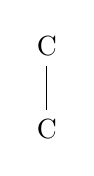
\begin{tikzpicture}[grow'=up]
		\Tree [.C C ] 					
		\end{tikzpicture}												&
		
		
		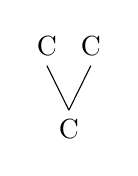
\begin{tikzpicture}[grow'=up]
		\Tree  [.C C C ];
		\end{tikzpicture}			
		&
		
		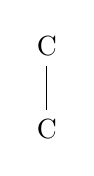
\begin{tikzpicture}[grow'=up]
		\Tree  [.C C ]
		\end{tikzpicture}
		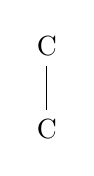
\begin{tikzpicture}[grow'=up]
		\Tree  [.C C ]
		\end{tikzpicture}		
	\end{tabularx}
	
	\caption{Autosegmental representation of geminates}
	 \label{fig:Autosegmental representation of geminates} 

\end{figure}

\figref{fig:Autosegmental representation of geminates} shows the autosegmental representations of singletons, \is{lexical gemination} lexical geminates and \is{morphological gemination} morphological geminates (for similar analyses see, for example,  \citealt[413]{Kenstowicz.1994}; \citealt[26f.]{Gussmann.2002} and \citealt[62]{Ridouane.2010}). The upper tier shows the skeletal tier and the lower one the segmental. While singletons only take one slot at both levels, \is{lexical gemination} lexical geminates occupy one slot at the segmental tier and two slots on the skeletal tier. The two prosodic slots account for the long duration of the geminate, as well as for its ambisyllabicity. The single slot on the segmental tier represents the {geminate's} inalterability and integrity. Since \is{morphological gemination} morphological geminates differ from \is{lexical gemination} lexical geminates in terms of their integrity and inalteribility, they take two slots on both tiers. This also mirrors their derivational nature, which naturally entails that a {morphological geminate} is made of two concatenated identical segments.


Differently from the autosegmental approach, the moraic approach does not entail a segmental prosodic tier on which the geminate is represented as having two slots. Instead, the root-node is directly connected to a higher prosodic structure, i.e. the mora, which represents a segment's underlying weight. \figref{fig:Moraic representation of geminates} shows the {moraic representation} of singletons, lexical and \is{morphological gemination} morphological geminates. While \is{lexical gemination} lexical geminates are underlyingly heavy, i.e. moraic, singletons are light, i.e. not moraic. Morphological geminates are represented as two identical singletons. These singletons are regarded as independent from each other and are therefore not underlyingly moraic  (for similar analyses see, for example,  \citealt[14]{Ham.2001}; \citealt[17]{Davis.2014} and \citealt{Davis.2017}).


\begin{figure} [h]
	\centering
	
	
	\begin{tabularx}{.8\linewidth}{YYY}
		
		&		lexical			 & 		 morphological \\
		
		singleton	&			  geminate	 & 			  geminate\\		
		\\
		\begin{tikzpicture}
		\Tree [.C  ] 					
		\end{tikzpicture}												&
		
		
		\begin{tikzpicture}[grow'=up]
		\Tree  [.C $\mu$ ]
		\end{tikzpicture}			
		&
		
		\begin{tikzpicture}[grow'=up]
		\Tree  [.C ]
		\end{tikzpicture}
		\begin{tikzpicture}[grow'=up]
		\Tree  [.C  ]
		\end{tikzpicture}		
		
	\end{tabularx}
	
	\caption{Moraic representation of geminates} 
	\label{fig:Moraic representation of geminates}
\end{figure}


Comparing the segmental and the moraic approach, it is striking that while the representation of \is{lexical gemination} lexical geminates differs between the two approaches, \is{morphological gemination} morphological geminates are represented as two underlying segments in both analyses.
In this book I will adopt this view and assume that the \isi{underlying representation} of \is{morphological gemination} morphological geminates consists of two segments. In word-medial position one of the segments is in coda position, the other forms the onset of the following syllable. 


While the \isi{underlying representation} of \is{morphological gemination} morphological geminates as two distinct segments seems undisputed, it is yet unclear how these two identical segments are realized at the phonetic level. As described in \sectref{Morphological Gemination}, only few studies on \isi{morphological gemination} exist. Most of these studies do not systematically investigate important lexical factors which might influence the realization of \is{morphological gemination} morphological geminates (e.g. morphological category and \isi{decomposability}). These factors are, however, important to look at since their role in {gemination} can provide us with important insights about the morpho-phonological, as well as as the \isi{morpho-phonetic interface} (see \chapref{Theory} for a thorough discussion). 
In this book, I will empirically investigate \isi{morphological gemination} with English affixes. I will systematically test which factors influence the \isi{phonetic realization} of \is{morphological gemination} morphological geminates with \is{un-}\prefix{un}, locative \is{locative in-}\prefix{in}, negative \is{negative in-}\prefix{in}, \is{dis-}\prefix{dis} and \is{-ly}\suffix{ly}, and thereby contribute new insights to the understanding of \is{morphological gemination} morphological geminates and morpho-phonological theory.


\section{Gemination in English} \label{Gemination in English}

The theoretical literature only sparsely discusses \isi{morphological gemination} in English. The phenomenon is mostly mentioned implicitly and rarely discussed in more than one sentence.  Assumptions about \isi{gemination} in English can, however, be gleaned from some  theoretically oriented studies and from secondary sources such as handbooks, textbooks or pronunciation dictionaries. Additionally it is possible to deduce predictions about gemination behavior of English affixes from morpho-phonological theories and psycholinguistic approaches of \isi{morphological processing}. In this section, I will restrict my discussion of English gemination to explicit mentions in the literature, as well as previous empirical studies on the topic. While I will concentrate on gemination with the affixes under investigation, I will also review general statements about gemination in English, i.e. I will take a look at mechanisms which are generally assumed to govern gemination in English, including gemination in compounds and phrases.
In \chapref{Theory}, I will then turn to prominent formal linguistic and psycholinguistic approaches, as well as prominent theories of speech production. I will discuss those approaches in detail, and deduce clear predictions about the gemination behavior of the affixes \is{un-}\prefix{un}, \is{in-}\prefix{in}, \is{dis-}\prefix{dis} and \is{-ly}\suffix{ly}.\footnote{An earlier version of this section was published in \cite{BenHedia.2017}.}
\label{assumptions}
 

\subsection{Assumptions } \label{assumption gem English}

 % Prinunciation dictionaries
I will start this review by looking at how pronunciation dictionaries (e.g. \citealt{Kenyon.1953, Roach.2011, Wells.2008}) treat \is{morphological gemination} morphological geminates in \is{un-}\prefix{un}, \is{in-}\prefix{in}, \is{dis-}\prefix{dis} and \hbox{-}\textit{ly}-affixed words.  There is a systematic difference between the representations of the prefix \is{in-}\prefix{in} and the prefix \is{un-}\prefix{un} in the dictionaries. If the prefix \is{un-}\prefix{un} is attached to a base starting in /n/, the word is transcribed with a long nasal (i.e. with [nː]). In contrast, if the prefix \is{in-}\prefix{in} attaches to a base starting with /n/, the transcription only shows a short /n/ (i.e. [n]). The only exception is the word \textit{innavigable} in \citet{Roach.2011}, where the word is transcribed with two [n]s. It is unclear what distinguishes this word from the other \is{in-}\prefix{in}prefixed words. 
  With \is{in-}\prefix{in}, there is the complication that the prefix has three additional variants that may or may not involve gemination: \is{im-}\textit{im-}, \textit{ir-} and \textit{il-}, as in \textit{immobile}, \textit{irresponsible} and \textit{illegal}, respectively. In the dictionaries one consistently finds a short consonant in these cases, too. That is, all \is{allomorphy}allomorphs of \is{in-}\prefix{in} are taken to behave in the same way with regard to {degemination}.
  
 For the prefix \is{dis-}\prefix{dis}, variation is found in \cite{Roach.2011}. While some types are transcribed with two fricatives (e.g. \textit{dissatisfy, dissimulation}), most types are transcribed with only one [s] (e.g. \textit{dissolution, dissemble)}. It is unclear on which bases it is decided whether a type is transcribed as featuring one or two consonants. There even is variation among types of the same root. While \textit{dissimulation} is transcribed with two [s]s, \textit{dissimulate} is transcribed with only one. Interestingly, in \cite{Roach.2011}  a long fricative (i.e. [s\textlengthmark]) is never assigned to \is{dis-}\prefix{dis}prefixed words. This suggests that, according to \cite{Roach.2011}, \is{morphological gemination} morphological geminates are realized differently in \is{dis-}\prefix{dis}prefixed words than in \is{un-}\prefix{un}pre\-fixed words. In contrast to doubles with \is{dis-}\prefix{dis}, doubles with \is{un-}\prefix{un} are transcribed with a long nasal (i.e. [n\textlengthmark])  instead of with two (i.e. [nn]).
 Differently from in \cite{Roach.2011}, in \cite{Wells.2008} there is no variation found for \textit{dis}-prefixed words. All types are transcribed with only one /s/, suggesting that \is{dis-}\prefix{dis} always {degeminates}. 
  
  For \is{-ly}\suffix{ly}-suffixed words, one finds an interesting note on gemination in \cite{Wells.2008}, stating that ``after a stem ending in l, one l is usually lost'' (451). \cite{Wells.2008} thus suggests that \hbox{-}\textit{ly}-suffixed words {degeminate}.

 
 Pronunciation dictionaries, which generally consider citation forms unaffected by context-specific or situation-specific influences, thus suggest gemination for \is{un-}\prefix{un} and {degemination} for \is{in-}\prefix{in} and \is{-ly}\suffix{ly}. For \is{dis-}\prefix{dis} the dictionaries do not agree. While one dictionary states that the prefix {degeminates} in all cases (\citealt{Wells.2008}), another one predicts cases in which at least some of the \is{morphological gemination} morphological geminates are pronounced as two consonants (\citealt{Roach.2011}).
 
 
Turning to the pertinent phonological or morphological literature, a similar picture emerges for the prefixes \is{un-}\prefix{un} and \is{in-}\prefix{in}, which are the most prominent, and hence the most discussed, examples for \isi{morphological gemination} in English. \citet[141]{Wijk.1966}; \citet[255]{OConnor.1973}; \citet[18]{Mohanan.1986}; \citet[119ff.]{Borowsky.1986}; \citet[111]{Catford.1988}; \citet[106]{Kreidler.1989}; \citet[251]{Ladefoged.1993}; \citet[18]{Harris.1994}; \citet[22]{Spencer.1996}; \citet[1055f.]{CohenGoldberg.2013}, and \citet{Cruttenden.2014} all agree that \is{un-}\prefix{un} geminates. Remarks on \is{in-}\prefix{in} are less frequent, and often only refer to isolated pertinent words, but those authors who mention the issue of double nasals with \is{in-}\prefix{in} all agree that \is{in-}\prefix{in} {degeminates} (\citealt[251]{Ladefoged.1993}; \citealt[18]{Mohanan.1986}; \citealt[18ff.]{Harris.1994}\mbox{;} \citealt[248]{Cruttenden.2014}; \citealt[1055f.]{CohenGoldberg.2013}).

The affixes \is{dis-}\prefix{dis} and \is{-ly}\suffix{ly} are far less frequently discussed in the literature. 
The adverbial suffix \is{-ly}\suffix{ly} is only mentioned implicitly in some of the literature mentioned above. In those works, derivatives with \is{-ly}\suffix{ly} are used as examples of words which geminate (cf. \citealt[141]{Wijk.1966}; \citealt[23]{Harris.1994}; \citealt[22]{Spencer.1996}). In contrast, \citet[82]{Bauer.2001}; \citet[353]{Giegerich.2012} and \citet[169]{Bauer.2013} claim variation with \is{-ly}\suffix{ly}. Some \is{-ly}\suffix{ly}-suffixed words are believed to geminate (e.g. \textit{stalely} and \textit{vilely}) and some are believed to {degeminate} (e.g. \textit{fully} and \textit{really}). For \is{-ly}\suffix{ly}-affixed words in which the suffix occurs after the suffix \suffix{al}, {degemination} is claimed (e.g.  \textit{federally}, \textit{globally}, \textit{spiritually}). \citet[169]{Bauer.2013} furthermore state that {degemination} is variable with yet some other words (e.g. \textit{dully} and \textit{wholly}). 
For the prefix \is{dis-}\prefix{dis}, there is no discussion which explicitly mentions the gemination behavior of the prefix. Assumptions about \is{dis-}\prefix{dis} can therefore only be gleaned from general statements about gemination in English, as well as from dictionary entries, which are, as described above, contradictory. 

After looking at specific mentions of the affixes in the literature, let us now turn to more general thoughts on gemination in English, i.e. the general mechanisms believed to govern gemination in English. 
Most of the discussed literature claims that the affix involved is decisive for the \isi{phonetic realization} of a double consonant. They assume gemination to be a categorical, i.e. not a gradient, phenomenon. The majority of approaches accounts for the alleged difference in gemination behavior between affixes by positing two different kinds of morphological boundary. \citet[18]{Mohanan.1986} and \citet[119ff.]{Borowsky.1986}, in the framework of Kiparskian lexical phonology (\citealt{Kiparsky.1982} et seq.), for example, assign \is{in-}\prefix{in} to \is{level 1 affix}{level 1} and \is{un-}\prefix{un} to \is{level 2 affix}{level 2}. In this theory, {level 1} affixes have weak morphological boundaries \is{boundary strength} which go along with greater phonological integration with their base, including assimilation and \isi{degemination}. Level 2 affixes, in contrast, form strong boundaries with their base and are phonologically less integrated. Hence, gemination is expected for {level 2} affixes. Similar in spirit is \citeauthor{Harris.1994}' (1994) account, in which the author distinguishes between root {affixation} (for \is{in-}\prefix{in}) and word {affixation} (for \is{un-}\prefix{un} and \is{-ly}\suffix{ly}). In root {affixation}, generally one phoneme is deleted when two identical segments immediately follow each other. 
\cite{CohenGoldberg.2013} attributes the alleged difference in gemination between \is{in-}\prefix{in} and \is{un-}\prefix{un} to their difference in  \isi{productivity}: the less productive prefix \is{in-}\prefix{in} \is{degemination}{degeminates}, while the more productive \is{un-}\prefix{un} geminates. 
\citet[354]{Giegerich.2012} proposes that gemination depends on the \is{phonological word} status of the derivative. The \isi{phonological word} status, similar to \isi{productivity}, mirrors \is{boundary strength}{morphological boundary strength}. Only derivatives with weak morphological boundaries form \is{prosodic word}{prosodic words} (see \sectref{prosodic word} for discussion). According to \cite{Giegerich.2012}, geminates only occur across \isi{prosodic word} boundaries, which is why most \is{-ly}\suffix{ly}-derivatives, which form a \isi{prosodic word} with their base, {degeminate}.

\citet[169]{Bauer.2013} describe gemination as less predictable, i.e.  not solely  predictable by the affix involved. They, in contrast to the approaches discussed above, assume variation within the gemination pattern of one affix. Furthermore, the authors point at possible variables, other than the affix, which could have an effect on gemination (e.g. speech tempo and the speaker). Similarly \citet[191, 288]{Giegerich.1992} notes the effect of \isi{speech mode} by stating that geminates are usually simplified in connected speech.
 
 
One can summarize that most of the theoretical literature, as well as pronunciation dictionaries, assume gemination to be affix-dependent. Different \is{boundary strength}{boundary strengths} between affixes are assumed to cause differences in gemination. While the nature of the boundary deviates between different approaches, the main idea is that stronger boundaries lead to gemination and weaker boundaries lead to \isi{reduction}, i.e. \isi{degemination}. Only few sources assume that factors other than the affix involved influence gemination, and that variation in gemination can be found in words compromising the same affix.  In \chapref{Theory}, I will return to the different ideas proposed and discuss them in more detail. 

Summarizing the affix-specific predictions, one can state that for \is{un-}\prefix{un} and \is{in-}\prefix{in}, pronunciation dictionaries, as well as the majority of the theoretical literature, agree that the former geminates, while the latter {degeminates}. Less is said about \is{dis-}\prefix{dis} and \is{-ly}\suffix{ly}. For \is{dis-}\prefix{dis}, dictionaries make contradicting assumptions and the theoretical literature is silent about its gemination behavior. For \is{-ly}\suffix{ly}, one also finds contradicting predictions. While \cite{Wells.2008} suggest {degemination} takes place, the majority of the theoretical literature claims gemination with \is{-ly}\suffix{ly}. Some of the literature predicts variation. 

\subsection{Previous empirical work}\label{previous empirical work}

Apart from \cite{BenHedia.2017}, which is given in \chapref{Corpus Studies}, there are five studies on gemination in English: \cite{Delattre.,Kaye.2005,Oh.2012,Oh.2013}   and \cite{Kotzor.2016}.   % Delattre
The first study by \cite{Delattre.} looked at word-boundary geminates. Delattre compared the duration of double consonants at word boundaries (such as the double nasal  in the sentence \textit{I've seen Nelly}) with word-final singletons (such as the nasal in \textit{I've seen Elly}) and word-initial singletons (such as the nasal in \textit{We see Nelly}). He investigated three different segments: /n/, /l/ and /s/. For all three he found that word-boundary geminates are longer than singletons. The nasal showed the highest \isi{degree of gemination} (singleton-geminate ratio: 1:1.5). The fricative and the lateral had a singleton-geminate ratio of 1:1.3. Interestingly, the duration of the preceding segment did not vary depending on the number of consonants. In other words, gemination did not affect preceding vowel duration.

Even though this study shows that \isi{morphological gemination} in English may lead to longer durations, it can only be regarded as a first clue to understand gemination in English. Since Delattre solely looked at word-boundary geminates, i.e. not at other types of morphological boundary, it remains unclear which role morphology, and consequently different \is{boundary strength}{boundary strengths}, actually plays in the realization of geminates. Furthermore, there are major methodological issues. Delattre's results are based on only a few types and it is thus unclear which role type-specific effects might have played. The study did furthermore not account for possibly intervening factors such as, for example, \isi{speech rate}. Another drawback of the study is its lack of appropriate statistics. Taking all of these drawbacks into account one can nevertheless assume that \isi{morphological gemination} at word boundaries in English does, at least in some cases, lead to gemination.


\citet{Kaye.2005} and \citet{Oh.2012} both empirically investigated gemination with the two English prefixes \is{un-}\prefix{un} and \is{in-}\prefix{in}. In both studies the gemination of \is{in-}\prefix{in}prefixed words was investigated by looking at words that featured the allomorph \textit{im-}. The reason for this is that there are very few \is{in-}\prefix{in}prefixed words with a base starting in /n/ (such as \textit{innumerous}), i.e. there are not enough different types to empirically investigate gemination with \is{in-}\prefix{in} (see \sectref{theory:in} for further discussion). 


\cite{Kaye.2005} investigated  only two \is{un-}\prefix{un}prefixed types (\textit{unknown, unnamed}) and one \is{in-}\prefix{in} prefixed type (\textit{immature}). In an elicitation task, ten speakers produced these words, as well as the words’ bases in isolation. Kaye then compared the durations of the nasals in the different words. The results indicate that both prefixes geminate. The [n] in \textit{unknown} is longer than the [n] in \textit{known},  the [n] in \textit{unnamed} is longer than the [n] in \textit{named} and the [m] in \textit{immature} is longer than the [m] in \textit{mature}. Kaye notes, however, that whether an \is{in-}\prefix{in}prefixed word geminates or not depends  on the individual speaker. Not all speakers produced the prefixed words with a longer nasal than the base. However, since Kaye did not apply any statistical analyses (beyond computing averages) and only investigated a very limited number of types, the results are somewhat inconclusive. What we can see, however, is that Kaye's empirical data go against the claim that \is{in-}\prefix{in} always {degeminates}.


\cite{Oh.2012} also investigated gemination with \is{un-}\prefix{un} and \is{in-}\prefix{in}, as well as gemination at word boundaries  (e.g. \textit{dim morning, one nail}). With regard to gemination with \is{in-}\prefix{in} and \is{un-}\prefix{un}, they compared the duration of \is{morphological gemination} morphological geminates with the duration of assumed phonological singletons in words starting with similar phonemic strings. The authors investigated 16 different words which contained two consonants in the orthographic representation.  The items were categorized  by Korean speakers (i.e. speakers of a language that has phonological geminates) who rated the duration of the nasals as either single or double, based on an English native speaker’s pronunciation of these words. The words \textit{immovable, immoral, immemorial, immeasured, unnoticed, unnamed, unnerve, unnail} were categorized as containing a double nasal, while \textit{ammonia, immensely, immunity, immigrational, annex, innate, annoyed, innerve} were categorized as words containing a single nasal. 
Additionally, Oh and Redford included word-boundary geminates (e.g. \textit{dim morning, one nail}) in their data set to investigate potential differences between word-internal and word-boundary geminates. All items were put into carrier sentences and read by eight participants in two different conditions (\isi{normal speech} vs. \isi{careful speech}). 

With regard to word-internal geminates the analyses showed that the items rated by Korean speakers as having double nasals were longer in duration than items rated as having single nasals. This indicates that at least some words with the prefix \is{in-}\prefix{in} show gemination.
However, there is variation in the gemination pattern of \is{in-}\prefix{in} found by \cite{Oh.2012}: the set of words with singletons mainly contains words that are morphologically simplex, but some words are not simplex. The word \textit{immigrational}, for example, is prefixed (compare \textit{migration}, \textit{immigration}), which in turn means that in this word, \is{in-}\prefix{in} {degeminates}, while in the other prefixed words it geminates. Note also that \is{in-}\prefix{in} in the word \textit{immigrational} (like, arguably, \textit{innate} `existing in a person [...] from birth', \textit{OED online}\nocite{OED.2013}, s.v. `innate, adj.'), has a locative meaning. Incidentally, both words in which we find \is{locative in-}\prefix{in} as a locative prefix ended up in the set of words that do not geminate, while the words with negative \is{in-}\prefix{in} showed gemination. This might hint at a systematic difference between locative and negative \is{negative in-}\prefix{in}, an issue that has so far never been discussed in the theoretical literature.

The study also reveals general differences between the two prefixes \is{un-}\prefix{un} and \is{in-}\prefix{in}. \cite{Oh.2012} found a difference in absolute nasal duration between the two prefixes. The nasal in \is{in-}\prefix{in}prefixed words is significantly shorter than the nasal in \is{un-}\prefix{un}prefixed words. This difference is more prominent in \isi{careful speech} than in \isi{normal speech}. The durational difference between the prefixes vanishes, however, in \isi{relative duration}. Relative duration refers to the nasal duration relative to the duration of the preceding vowel. This means that not only nasal duration differs between the two prefixes but that there is also a difference in preceding vowel duration. The prefix \is{un-}\prefix{un} features a longer vowel than the prefix \is{in-}\prefix{in}.  In other words, \is{un-}\prefix{un} is generally longer than \is{in-}\prefix{in}. In addition to prefix duration, \cite{Oh.2012} also found non-durational differences between \is{un-}\prefix{un} and \is{in-}\prefix{in}. In \isi{careful speech}, speakers sometimes inserted a pause between the two nasals of \is{un-}\prefix{un}prefixed words, whereas a pause was never inserted in \is{in-}\prefix{in}prefixed words. The authors interpret the inserted pause as a boundary cue.

Turning to word-boundary geminates,  results revealed that there was no durational difference in \isi{absolute duration} between word-internal and word-boundary geminates. There was, however, a difference between the two types of geminates in \isi{relative duration}. Word-boundary geminates were shorter than word-internal geminates, and as long as singletons in \isi{relative duration}. In other words, while geminates in \is{un-}\prefix{un} and \is{in-}\prefix{in}prefixed words are longer than singletons in absolute and \isi{relative duration}, word-boundary geminates are only longer than singletons in \isi{absolute duration}.


Oh and Redford interpret their results as evidence that word-boundary geminates are represented differently than word-internal geminates, i.e. that gemination is influenced by \isi{boundary strength}.  Furthermore, they argue that the prefix \is{un-}\prefix{un} might be represented differently than the prefix \is{in-}\prefix{in}. They base their argument on the finding that, even though there does not seem to be a systematic difference in the gemination behavior of the two prefixes, the two prefixes display differences in their overall duration, as well as differences with regard to non-durational boundary cues. \cite{Oh.2012} venture the idea that different affix representations emerge from differences in \isi{boundary strength} (cf. \citealt{Kiparsky.1982,Mohanan.1986}, see \sectref{LexPhon} for discussion), or from differences in \isi{productivity} and \isi{segmentability} (cf. \citealt{Hay.2003}, see \sectref{Morphological Gemination: Implications for Psycholinguistic Theories of Morphological Processing} for discussion). Since the prefix \is{un-}\prefix{un} has a stronger boundary than \is{in-}\prefix{in}, and since it is more productive and segmentable, there is less \isi{reduction} with \is{un-}\prefix{un} than with \is{in-}\prefix{in}, i.e. it is longer and features boundary cues.


To investigate the relation of different morphological boundaries and gemination further, in a follow-up study \cite{Oh.2013} investigated whether there is a difference between geminates at compound-internal boundaries (e.g. \textit{homemade}) and geminates at word boundaries (e.g. \textit{room maid}). The comparison of geminate durations and the duration of singletons at word boundaries (e.g. \textit{dough made}) showed that both types of geminates are longer than singletons. A significant difference between compound-internal and word-boundary geminates is only found in \isi{careful speech}, and only in \is{absolute duration}{absolute consonant duration}. In accordance with the idea that word-boundary geminates have a stronger morphological boundary than compound-internal geminates,  in \isi{careful speech} word-boundary geminates are longer. In \isi{normal speech} the difference vanishes. For \isi{relative duration}, there never is a difference between compound-internal and word-boundary geminates. \cite{Oh.2013} interprets the results as there not being a difference in the realization of compound-internal and word-boundary geminates in English. 


Thus, while in \cite{Oh.2012} there might be some indication for effects of \isi{boundary strength} on gemination (difference between word-internal and word-boundary geminates in \isi{relative duration}), we do not find these effects in \cite{Oh.2013}. There are various possible explanations. 
It might for example be that only certain boundary differences lead to differences in gemination. This explanation ties in with the results on \isi{morphological gemination} in German, Tashlhiyt Berber and Maltese discussed in \sectref{Morphological Gemination}. These studies also showed that, while gemination differed between some types of boundaries, it did not between others. 
Another explanation for the deviating results might be related to the studies' methodologies.  
Both studies only investigated a very small number of types, which made it impossible to test the influence of type-specific factors on duration. Furthermore, there might be other intervening factors such as, for example, \isi{speech rate} and speaker, which influence duration, and which were not systematically  taken into account. 
With regard to methodology, another crucial aspect must be considered when interpreting the results.
The studies show differences in effects depending on the acoustic correlate used as the measure of gemination. Effects are different for absolute and \isi{relative duration}. There are also differences depending on speech condition, i.e. careful vs. \isi{normal speech}. 
Especially the different outcomes depending on speech condition suggest that factors related to the experimental set-up influence results of durational studies to a great degree. It is yet unclear how to interpret the relation between the different outcomes and the different conditions.
To shed light on the matter, it is necessary to conduct further studies which systematically compare experimental data with \isi{conversational speech}, and which control for intervening factors in a systematic way. More advanced statistics, which are able to tease apart different effects, are necessary to explain which factors cause which durational differences, and whether it is indeed \isi{boundary strength} which leads to differences in gemination between different words and constructions.


\largerpage
The most recent study on gemination in English looked at gemination in {suffixation} and compounding. Using a reading experiment, \cite{Kotzor.2016} investigated the two suffixes \is{-ly}\suffix{ly} and \suffix{ness}, as well as compounds with sonorant ([l] and [n]) and stop geminates ([p], [t] and [k]). With respect to the suffixed data, they compared the double consonant with the singleton in the pertinent base word to which the suffix \textit{-er} was added. Hence, the double consonants in \suffix{ness}- and \is{-ly}\suffix{ly}-suffixed words (e.g. /nn/  and /ll/ in \textit{coolly} and \textit{meanness}) were compared to the pertinent singletons in \textit{-er}-suffixed words (e.g. /n/ and /l/ in \textit{meaner} and \textit{cooler}). The doubles in compounds (e.g. /nn/ in \textit{pine nut}) were compared to singletons in similar compound words (e.g. /n/ in \textit{pineapple}). 
The results reveal that both types of geminates, i.e. suffixational and compound geminates, are longer than the pertinent singletons. There was no effect of the geminate on the preceding vowel duration, neither for the suffixes, nor for the compounds. Thus, \cite{Kotzor.2016} did not find a significant difference between the gemination of suffixes and compounds. 

\largerpage Unfortunately, \cite{Kotzor.2016} do not provide a separate analysis for each of the two suffixes. In other words, their analysis does not provide the possibility to state whether the suffixes \suffix{ness} and \is{-ly}\suffix{ly} behave differently with regard to their gemination behavior. This can be regarded as a major drawback of the study since, as described in \sectref{assumptions}, it is commonly assumed that gemination is affix-dependent. From a theoretical point of view, there is good reason to assume that the two suffixes \is{-ly}\suffix{ly} and \textit{-ness} do not behave identically. 
This idea is further supported by the fact that geminate duration varies among different types of consonants (cf. \sectref{what is gemination}). The lateral in \is{-ly}\suffix{ly}-words is expected to inherently show different durations than the nasal in \textit{-ness}-words. Furthermore, there might be structural differences between the two affixes, such as their \isi{segmentability} and \isi{boundary strength}, which might lead to different behavior regarding gemination. 
An additional problem with the study is the limited number of types investigated. For each affix only six types with a {morphological geminate} were included, making it impossible to investigate type-specific effects such as word-form \isi{frequency} or a word's individual \isi{decomposability}. Thus, even though the study provides some evidence for the gemination of \is{-ly}\suffix{ly} and \suffix{ness}, one must be cautious to interpret the results. Further research on the individual suffixes incorporating a greater number of different types is necessary to make reliable statements about their gemination behavior.


To summarize, previous research on gemination in English leaves us with a number of unsolved problems. First, there is only little empirical evidence available and the few studies which do exist differ significantly in their methodology and the constructions they investigated. Hence, the facts essentially are unclear. Only three studies looked at affixational gemination in English, i.e. the phenomenon under investigation in this book (\citealt{Kaye.2005, Oh.2012, Kotzor.2016}). Two of these studies (\citealt{Kaye.2005, Oh.2012}) call the assumption that \is{in-}\prefix{in} {degeminates} into question, and hence demonstrate the need for further testing of widely-held beliefs about gemination in English. 

Second, existing empirical studies are rather limited in their data sets and consider only words spoken under experimental conditions, i.e. in isolation or in carrier sentences. What is lacking is data from \isi{natural speech}. As pointed out in the literature (e.g. \citealt{Giegerich.1992, Bauer.2013}), and as evidenced by \cite{Oh.2012} and \cite{Oh.2013}, the mode of speech might significantly influence the realization of \is{morphological gemination} morphological geminates. Therefore, it is necessary to investigate the phenomenon in various conditions, making it possible to compare \isi{natural speech} with experimental data. This will allow us to find out which factors influence gemination on which level.

Third, existing studies have not simultaneously considered different influences which might affect gemination, but rather concentrated on one specific aspect, i.e. they neglected other possibly intervening factors. None of the studies described above looked at word-specific factors, such as word-form \isi{frequency} or a word's individual \isi{decomposability}. Even though, as shown in \sectref {assumptions}, most claims about gemination are based on morphological categories, morphological factors were only considered sparsely in previous research. While most studies pointed out that different morphological categories, such as different affixes or derivatives with varying \is{boundary strength}{morphological boundary strength}, might differ in their gemination behavior, their methodology was insufficient to shed light on the matter. 
The studies comparing \is{un-}\prefix{un} and \is{in-}\prefix{in}, for example, just assumed a categorical difference in \isi{boundary strength} between the two affixes. This assumption needs to be empirically investigated. Furthermore, the investigation of \is{in-}\prefix{in} did not consider that there are two different \is{in-}\prefix{in}prefixes, i.e. locative and negative, and that there are potential differences between them. The study on the two suffixes \is{-ly}\suffix{ly} and \textit{-ness} did not differentiate between the two suffixes at all, just assuming a similar behavior of both of them. 

To conclude, previous research hinted at some interesting effects, such as the gemination of affixes which are assumed to {degeminate}, and differences in gemination depending on the type of morphological boundary involved. However, due to mainly methodological reasons further research is needed to clarify the facts.


%  
\chapter{The Affixes under investigation}{\label{affixes}}


In this chapter I will describe the five affixes \prefix{un}, negative \prefix{in}, locative \prefix{in}, \prefix{dis} and \suffix{ly} using the relevant morphological and phonological literature. I will discuss their phonological behavior, as well as important morphological, semantic and lexical properties, and compare them with regard to these factors.

Before discussing the affixes, I will give a brief overview of the factors which lead to their inclusion in this study.
The prefixes \is{un-}\prefix{un} and \is{in-}\prefix{in} were included because of two reasons.
First, they are the most prominent examples of \is{morphological gemination}{gemination}/\isi{degemination} given in the literature (see discussion in \sectref{assumptions}).  Second, they are investigated empirically in two previous studies, i.e. a comparison to previous results is possible. 
To investigate an additional prefix, and to also take a look at {gemination} in suffixes, the affixes \is{dis-}\prefix{dis} and \is{-ly}\suffix{ly}  were added to the data set. The choice to include these two affixes was on the one hand due to their comparatively high type \isi{frequency}, which allows for testing type-specific effects on {gemination}, and  on the other due to their phonological and morphological make-up.
The five affixes partly overlap in their characteristics, such as their semantics, their prosodic make-up and their \isi{segmentability}. Importantly, they also show some major differences in their features. This combination of similarities and differences between the affixes makes it possible to test various factors which potentially affect \is{morphological gemination} across affixes.

In the following, I will describe the formal and structural characteristics of each affix, lay out their phonological and prosodic behavior, and discuss their semantics. Since the literature is often not very specific, or even contradictory when discussing certain aspects of \isi{affixation} (e.g. \isi{stress} pattern or \isi{productivity}), it is often not possible to give a clear-cut description of a certain affix and its behavior. I will remain neutral regarding most of the controversial issues but lay out the different possibilities, as found in the literature.  

After looking at each affix in isolation, I will compare the five affixes with each other. It is of prime importance to look at the differences between the affixes, since these differences lead, according to the theories discussed, to different predictions for their gemination behavior. I will pay special attention to \isi{boundary strength} as it is one of the most important factors for predicting \is{morphological gemination}{gemination}.  
At the end of this section, I will provide some insightful figures regarding the scope of the phenomenon across affixes. In other words, I will lay out how many types with a \is{morphological gemination}{morphological geminate} exist for each affix.

\section{Description of the affixes}

\subsection{The prefix \prefix{un}} {\label{description un}}

The affix \is{un-}\prefix{un} is a native prefix which takes native and non-native bases. According to \citet[ 355, 361, 371ff.]{Bauer.2013}, its bases can be verbs, nouns and adjectives. The prefix rarely changes the category of its base and does not take bound roots. It is one of the most productive prefixes in English and has a clearly negative meaning, which varies slightly depending on the base it attaches to. On verbs its meaning is reversive (e.g. \textit{screw} vs. \textit{unscrew}) and sometimes privative (e.g. \textit{dress} vs. \textit{undress}), on adjectives its meaning is contrary or contradicting (e.g. \textit{cool} vs. \textit{uncool}), and on nouns it mostly is privative (e.g. \textit{faith} vs. \textit{unfaith}).
In general, the meaning of \is{un-}\prefix{un}derivatives is very transparent. Only few forms exist in which one cannot deduce a derivative's meaning by adding the negative meaning of \is{un-}\prefix{un} to that of its base (e.g. \textit{unorthodox}).

Turning to the prefix's phonological attributes, \is{un-}\prefix{un} shows what can be called ``optional assimilation''. This assimilation affects \is{un-}\prefix{un}derivatives with a base starting in a bilabial (e.g. \textit{unplugged, unbreakable, unmarried}) and \is{un-}\prefix{un}derivatives with a base starting in a velar plosive (e.g. \textit{ungrateful, uncool}).
Before bilabials the prefix-final nasal sometimes is realized as [m]. Before velar plosives the prefixal nasal sometimes is velarized, i.e. realized as [ŋ] (cf. \citealt[5f.]{Hanote.2010}; \citealt[180]{Bauer.2013}; \citealt[125]{Okada.2013}). 
This optional assimilation is not mirrored in \isi{orthography} and, according to \citet[125]{Okada.2013}, is purely phonetic, i.e. not phonological, in nature. \citet[87f.]{Stockwell.2001} explain the optional assimilation of \is{un-}\prefix{un} by a conflict between ``ease of pronunciation'' and ``transparency''. While the assimilation of the nasal makes pronunciation easier, the transparent nature of the prefix blocks its total assimilation.
Except for one study (\citealt{Hanote.2010}), there is, according to my knowledge, no empirical work on the assimilation of English \is{un-}\prefix{un}. \cite{Hanote.2010} found no systematic pattern with regard to assimilation with \is{un-}\prefix{un}. However, since the authors restricted their study on dictionary data it is questionable how generalizable their results are.  
As \citet[138]{Raffelsiefen.1999}, for example, proposes, assimilation with \is{un-}\prefix{un} might be sensitive to register.  According to her,  assimilation is most likely to occur in fast, \is{conversational speech}{casual speech}. This would mean that dictionary data is not suited to investigate the matter.
To conclude, \is{un-}\prefix{un} sometimes assimilates but the pattern of its assimilation is yet unclear.




Before discussing the \isi{stress} status of \is{un-}\prefix{un}, a general note on prefix \isi{stress} is in order. The \isi{stress} of prefixes is not well researched and observations are mostly anecdotal, i.e. rely on individuals' intuitions rather than on empirical studies. Furthermore, as evidenced in \cite{Videau.2015}, prefixal stress depends on various factors, such as \isi{semantic transparency}, syntactic context and extra-linguistic context. It is yet unclear how these factors interact, i.e. it is unclear how exactly they influence \isi{stress} with prefixes.
Even when leaving contextual influences aside, i.e. when concentrating on lexical \isi{stress} in isolated words, it is quite difficult to determine the \isi{stress} pattern of prefixed words. 

The determination of \isi{stress} for monosyllabic prefixes, such as \is{un-}\prefix{un}, \is{in-}\prefix{in} and \is{dis-}\prefix{dis}, is of special difficulty. When followed by an unstressed syllable, they are, due to prosodic constraints, usually taken to be \is{stress}stressed. Matters are, however, more complicated when the prefix is followed by a \is{stress}stressed syllable. In those cases it is very challenging to determine the relative prominence relations between the prefix and the base-initial syllable, i.e. it is very hard to determine whether the prefix is \is{stress}stressed or not. 
While it is generally assumed that prefixes can bear \isi{stress}, it is unclear how \isi{stress} patterns in those cases. In other words, it is unclear whether the prefix is unstressed, whether it bears primary \isi{stress} or whether it bears secondary \isi{stress}. As discussed in \citet[126]{Okada.2013} for \is{un-}\prefix{un}, \prefix{in} and \textit{non-}, there is variation within prefixes, and this variation ``leads linguists to different descriptions''. 
To summarize, due to difficulties in determining \isi{stress} and the not well researched variation in prefix \isi{stress}, the descriptions of prefixal stress deviate between sources for the prefixes \is{un-}\prefix{un}, \prefix{in} and \is{dis-}\prefix{dis}. %The \isi{stress} pattern of the prefixes is unclear.


The available descriptions of \isi{stress} with \is{un-}\prefix{un} reflect the problems just pointed out. While \citet[4]{Allen.1978} notes that the prefix never bears \isi{stress}, other sources such as \citet[464f.]{Jespersen.1965} and \citet[126]{Okada.2013} state that \is{un-}\prefix{un} is a stress-preserving prefix that may carry \isi{stress}. Similarly in \cite{Wells.2008} \is{un-}\prefix{un} can be \is{stress}stressed. Except for \cite{Allen.1978}, all sources agree that \is{un-}\prefix{un} is \is{stress}stressed if the base-initial syllable of the pertinent derivative is unstressed (e.g. \textit{ˌunconˈventional}\footnote{Throughout this book I will use ˈ to mark primary \is{stress}stressed syllables and ˌ to mark secondary \is{stress}stressed syllables.}).
Assumptions deviate for those cases in which the first syllable of the derivative's base is \is{stress}stressed (e.g. \textit{unˈjust}). \citet[464f.]{Jespersen.1965} notes for these cases that, while in some of the most common \is{un-}\prefix{un}derivatives the prefix is unstressed (e.g. \textit{unˈcommon, unˈhappy}), in most cases the prefix is \is{stress}stressed (e.g. \textit{ˈunˈaided, ˈunˈjust}). 
In \citet[808]{Wells.2008} it is noted that, while generally the prefix may be either \is{stress}stressed or unstressed in those cases, verbs always have a \is{stress}stressed prefix (e.g. \textit{ˌunˈcoil}). Furthermore, it is noted that \is{un-}\prefix{un} ``is unstressed particularly where it is not a true prefix (\textit{unˈwieldy})'' (808). Wells does not give a definition of true prefixhood though, i.e. this statement is quite unclear. Divided or uncertain usage is annotated for some of the \is{un-}\prefix{un}prefixed words with a \is{stress}stressed base-initial syllable (e.g. \textit{\textsubscript{(}ˌ\textsubscript{)}unˈbearable, \textsubscript{(}ˌ\textsubscript{)}unˈleash}). As evidenced in a study by \citet[2ff.]{Hanote.2010}, the assignment of prefixal stress with \is{un-}\prefix{un} in \cite{Wells.2008} does not follow any systematic pattern.
One can thus state that the literature does not provide clear, systematic and empirically-based criteria for \isi{stress} in derivatives with a \is{stress}stressed base-initial syllable. It therefore remains unclear when \is{un-}\prefix{un} is \is{stress}stressed and when it is unstressed. 


One can summarize that \is{un-}\prefix{un} is a very segmentable and very productive prefix. Its meaning is clearly negative and transparent in the vast majority of derivatives. The fact that \is{un-}\prefix{un} only optionally assimilates can be interpreted as a result of its high \isi{segmentability} which blocks total assimilation, and  which hence ensures the prefix's phonological independence from its base. With regard to \isi{stress}, one can state that \is{un-}\prefix{un} can bear \isi{stress} but that the \isi{stress} pattern of the prefix is yet unclear.



\subsection{The prefix \prefix{in}} \label{theory:in}

When investigating the prefix \is{in-}\prefix{in}, one must acknowledge the existence of two different \prefix{in}prefixes in English: \is{negative in-}negative \prefix{in} and \is{locative in-}locative \prefix{in}. While the existence of \is{negative in-}negative \prefix{in} is uncontroversial, the idea of \is{locative in-}locative \prefix{in} may not be as straightforward. The reason is that \is{locative in-}locative \prefix{in} often occurs in derivatives with bound roots, such as \textit{inject} or \textit{infuse}. In these words the discrete meaning of \prefix{in}, as well as the discrete meaning of the base, is often unclear. This might lead to the view that locative \textit{in-} is not a prefix but some sort of unit below the word level with  no clear semantic content. This view, however, neglects that \is{locative in-}locative \prefix{in} does indeed have a stable meaning.  

Let us take the standard methodological approach to morphological categories according to which an affix should have an identifiable, stable meaning across different words (cf., for example, \citealt[Chapter 5.2.2]{Plag.1999}; \citealt[63ff.]{Stockwell.2001}; \citealt[68]{Schulte.2015}). Under this approach, we would consider \prefix{in} a locative prefix in all those words (and only in those) where the word-initial string \prefix{in} can be assigned some locative meaning and where at the same time the remaining string is also attested outside that word with a stable, identifiable meaning.
Implementing this method, we would be able to assign some locative meaning to the string \prefix{in} in words such as \textit{infuse} `to pour in', \textit{implant} `to plant in' and \textit{import} `to bring in' (\textit{OED online} paraphrases). The remaining strings, i.e. the bases, in these words are all attested (either as words or as bound roots) outside these words with sufficiently similar meaning (cf. \textit{transfuse}, \textit{plant}, \textit{export}). This small sample thus shows that, at least in some words, there is a locative prefix \prefix{in}. 


In this study, all words in which the affix and the base carry a stable meaning are considered as morphologically complex.  Since, complex words with both \prefix{in}prefixes exist, i.e. negative and \is{locative in-}locative \prefix{in}, both types of \is{in-}\prefix{in} are included in the study.  Below I will take a closer look at each type of \prefix{in}.




\subsection{Negative \prefix{in} } \label{negative in}

Differently from \prefix{un}, \is{negative in-}negative \prefix{in} is a non-native (or Latinate) prefix that takes non-native bases. It mostly takes adjectives as its base (e.g. \textit{intolerant, immortal}). Only sometimes nouns are taken as its base (e.g. \textit{inexperience}).  In most cases, \is{negative in-}negative \prefix{in} does not change the word class of its derivative.  Usually free bases are found with \is{negative in-}negative \prefix{in} (e.g. \textit{intolerant, impossible}), but in some derivatives bound roots are found (e.g. \textit{inept, innocent}). In these words it is, however, questionable whether \prefix{in} can even be considered a prefix (cf. \citealt[356f., 611]{Bauer.2013}).

The majority of the literature claims that \is{negative in-}negative \prefix{in} is not productive (cf. \citealt[1688]{Bauer.2002}). A search of hapax legomena in the Corpus of Contemporary American English (\citealt{Davies.20082014}), as carried out by \citet[361]{Bauer.2013}, reveals however that there is indeed a number of new derivatives with negative \textit{in}-. Examples are \textit{immedical, inactual, inconservative} and \textit{inextractable}.  One should note, however, that \is{negative in-}negative \prefix{in} is far less productive than \prefix{un}, which carries similar meaning. Both prefixes denote contrary or contradictory meaning on adjectives.
 Because of these similarities in meaning the prefixes are often treated as rivals. It is often claimed that the existence of a derivative featuring one of the two prefixes blocks the existence of  a derivative with the other. According to this view, the existence of the word *\textit{inhappy}, for example, is blocked by the existence of the word \textit{unhappy} (see, for example,  \citealt[467ff.]{Jespersen.1965}; \citealt[1688f.]{Bauer.2002} and \citealt[377ff.]{Bauer.2013} for discussion).  
As reported by \citet[377]{Bauer.2013}, the idea of rivalry between the two prefixes is, however, invalidated by the existence of derivatives such as \textit{inaccessible} and \textit{unacessible}. There is no noticeable difference in meaning between the two derivatives, and in turn there is no difference in meaning between the two prefixes \is{un-}\prefix{un} and \prefix{in}.
However, while the two prefixes often are identical in meaning, \citet[379]{Bauer.2013}, similar to  \cite{Jespersen.1965} and \cite{Bauer.2002},  note that \prefix{in}derivatives are more often lexicalized than derivatives with \prefix{un}. To summarize, while \is{negative in-}negative \prefix{in} is very similar to \prefix{un} in its meaning, it does not share its high degree of \isi{productivity} and its consistency with regard to \isi{semantic transparency}.

Turning to the phonological features of \is{negative in-}negative \prefix{in}, one must mention its obligatory assimilation. Before a bilabial the prefixal nasal becomes /m/. Before a base-initial lateral the nasal becomes /l/, and before an alveolar rhotic it becomes /r/. Examples are \textit{impossible}, \textit{immortal}, \textit{illogical} and \textit{irregular} (cf. \citealt[1687]{Bauer.2002}; \citealt[359]{Bauer.2013}; \citealt[123f.]{Okada.2013}). This assimilation is also mirrored in \isi{orthography}. 

With regard to \isi{stress}, \prefix{in}, similar to \prefix{un}, is generally assumed to be \is{stress}stressed when followed by an unstressed syllable (cf. \citealt[473]{Jespersen.1965}; \citealt[381, 384]{Wells.2008};  \citealt[183]{Bauer.2013}; \citealt[126]{Okada.2013}). Examples are \textit{ˌinexˈhaustible, ˌindeˈscribable} and \textit{ˌimmeˈmorial}. In those cases \prefix{in} bears secondary \isi{stress}. There are also some derivatives, such as \textit{ˈimpotent} and \textit{ˈimpious}, in which \prefix{in} is primarily \is{stress}stressed. \citet[183]{Bauer.2013} note that while  \isi{stress} with \prefix{in} seems unsystematic in general,  the prefix seems to only bear primary \isi{stress} when the base of the derivative is bound.
In case of a \is{stress}stressed base-initial syllable, \prefix{in} is, in contrast to \prefix{un}, generally taken to be unstressed (cf. \citealt{Wells.2008}; \citealt[183]{Bauer.2013}; \citealt[126]{Okada.2013}). 

We can summarize that, while \is{negative in-}negative \prefix{in} is similar in meaning to \is{un-}\prefix{un}, it is less semantically and phonologically transparent. It is also less productive. Negative \prefix{in} has more bound roots than \is{un-}\prefix{un}, is sometimes semantically opaque, and derivatives are more often lexicalized. The prefix is phonologically more integrated in its base than \is{un-}\prefix{un}. This is indicated by the obligatory assimilation of the prefix. The \isi{stress} pattern of \prefix{in} can also be interpreted as an indicator of its phonological integration. While in some respects the \isi{stress} pattern is similar to the one of \is{un-}\prefix{un}, the prefix, contrary to \is{un-}\prefix{un}, also bears primary \isi{stress} in some cases. Primary \isi{stress} emerges with bound roots and denotes \isi{stress shift}, i.e. in those derivatives the position of primary \isi{stress} has shifted from the base to the prefix. This shows that the boundary between prefix and base is rather weak.\\


\subsection{Locative \prefix{in}} \label{locative in}

Locative \prefix{in} differs in interesting respects from \is{negative in-}negative \prefix{in}. Differently from negative \prefix{in}, the origin of \is{locative in-}locative \prefix{in} is twofold. This leads to a prominent distinction in the literature. Traditional approaches differentiate between non-native (or Latinate) \is{locative in-}locative \prefix{in} and native \is{locative in-}locative \prefix{in}.  While the first one is commonly analyzed as a prefix which takes non-native bases, the second is often analyzed as a locative particle (cf. \citealt[497ff.]{Jespersen.1965}; \citealt[115,163f.]{Marchand.1969}; \citealt[1685]{Bauer.2002}). Examples are given below:

\begin{exe}
	\ex non-native locative \prefix{in}: \hspace{0.7cm} \textit{inject, immigrate, impress}
	\ex native locative \prefix{in}: \hspace{1.4cm} \textit{inborn, inbreed, indoors}
\end{exe}

\cite{Bauer.2013} also make a distinction between the two different cases but regard both types of \is{locative in-}locative \prefix{in} as prefixes. Since the authors only discuss productive prefixes, and since they consider non-native \is{locative in-}locative \prefix{in} unproductive,  only native \prefix{in} is discussed in their work. It is said to be a productive prefix that attaches to nouns, adjectives and verbs. It takes native and non-native bases (\citealt[334, 340]{Bauer.2013}).
 
 It is generally assumed that the two types of \is{locative in-}locative \prefix{in} differ in their type of base, their \isi{productivity} and in the degree of phonological assimilation they display. While the non-native prefix is believed to mostly take non-native bases (see \citealt[499]{Jespersen.1965}), native \prefix{in} also attaches to native bases (see \citealt[334]{Bauer.2013}). While non-native \is{locative in-}locative \prefix{in} is not productive, the native form is believed to be productive. With regard to phonological assimilation, non-native \is{locative in-}locative \prefix{in} undergoes the same obligatory assimilation as negative \prefix{in}, while native \is{locative in-}locative \prefix{in} is described as only optionally assimilating (see \citealt[499]{Jespersen.1965}; \citealt[335]{Bauer.2013}). The common assumption thus seems to be that non-native \is{locative in-}locative \prefix{in} is phonologically and semantically less transparent than native \is{locative in-}locative \prefix{in}. There are, however, no empirical studies investigating whether these criteria mirror the distinction between the two types of \is{locative in-}locative \prefix{in}. 
 

It is not easy to distinguish between native and non-native \is{locative in-}locative \prefix{in}. This problem is  already discussed in early works such as \citet[499]{Jespersen.1965} and \citet[164]{Marchand.1969}. The semantics of both types of \is{locative in-}locative \prefix{in} overlap to a high degree. Both prefixes denote a locative meaning, which is formulated as ‘into, in, within; on, upon; towards, against’ in the \textit{OED online}\nocite{OED.2013}. The \textit{OED} further mentions that 

\begin{quote}
[s]ince \prefix{in} prefix 1 [non-native \prefix{in}] and \textit{in-} prefix 2 [native \prefix{in}] are identical in form, and to a great extent in sense, they come in later use to be felt as one and the same prefix; and it is this resulting prefix which appears in many words of later formation.
\end{quote}

It is thus suggested that, while \is{locative in-}locative \prefix{in} has two origins, the distinction between the two formerly distinct types of \is{locative in-}locative \prefix{in} is no longer clear. This is in line with the observation that the criteria used to distinguish native from non-native \is{locative in-}locative \prefix{in} are rather blurry. 
In this study, I will not explicitly distinguish between the two types of \is{locative in-}locative \prefix{in}. I will, however, account for differences in \isi{semantic transparency}, phonological make-up and type of base in my studies. I therefore will be able to implicitly differentiate between more \is{decomposability}decomposable and less \is{decomposability}decomposable \is{locative in-}locative \prefix{in}derivatives, which in turn, according the literature, may mirror the distinction between native and non-native \is{locative in-}locative \prefix{in}.

With regard to \isi{stress}, the literature is mostly silent about a distinctive \isi{stress} pattern for \is{locative in-}locative \prefix{in}. Except for \citet[384]{Wells.2008}, who notes that \prefix{in} is ``generally \is{stress}stressed only
(i) if meaning `in' rather than `not''', there are no explicit mentions about the \isi{stress} pattern of \is{locative in-}locative \prefix{in}. While, according to \cite{Wells.2008}, \is{locative in-}locative \prefix{in} is \is{stress}stressed and \is{negative in-}negative \prefix{in} is not, there are also sources which state that \is{negative in-}negative \prefix{in} can be \is{stress}stressed (see description of negative \prefix{in} above). It is thus unclear whether there is a systematic difference between the \isi{stress} pattern of locative and negative \prefix{in}. One could venture the idea that \is{locative in-}locative \prefix{in}, due to its assumingly higher \isi{frequency} of bound roots, more often bears primary \isi{stress} than negative \prefix{in}. This would fit in with \citeauthor{Wells.2008}'s statement. It, however, is an assumption that calls for empirical evidence.

To summarize, \is{locative in-}locative \prefix{in} is of two different origins which makes it rather difficult to make clear statements about the prefix. It seems that it occurs quite frequently with bound bases, is often semantically opaque and less productive than negative \prefix{in}. In other words, \is{locative in-}locative \prefix{in} seems to have a weaker morphological boundary than negative \prefix{in} and \is{un-}\prefix{un}. This impression is, however, to be tested empirically.

 
\subsection{The prefix \prefix{dis}}

The prefix \is{dis-}\prefix{dis} is a non-native (or Latinate) prefix that takes mostly native bases. Occasionally non-native bases are found in \is{dis-}\prefix{dis}derivatives (e.g. in the word \textit{disbelief}). The prefix takes mostly verbs and nouns as its base, sometimes adjectives. It is rarely category-changing and mostly takes words as its bases (see \citealt[481]{Jespersen.1965}; \citealt[158ff.]{Marchand.1969}; \citealt[355, 357]{Bauer.2013}).
According to \citet[358]{Bauer.2013}, the few \is{dis-}\prefix{dis}derivatives with bound roots, such as \textit{distort}, came to English as borrowings. Furthermore, the authors state that these borrowed words differ in their phonological structure from the other \is{dis-}\prefix{dis}words (e.g. in their \isi{stress} pattern).


As negative \prefix{in} and \prefix{un}, the prefix \is{dis-}\prefix{dis} denotes negativity.  With adjectives \is{dis-}\prefix{dis} is, similar to \is{un-}\prefix{un} and \prefix{in}, contrary or contradictory (e.g. \textit{dishonest}). It is only in this category that \is{dis-}\prefix{dis} is productive (see \citealt[358]{Bauer.2013}). With nominal bases \is{dis-}\prefix{dis} is privative (e.g. \textit{disbelief}). With verbs it often is privative or reversative (e.g. \textit{disconnect} or \textit{disarm})  (see \citealt[372, 375]{Bauer.2013}).
Because of the similarities in meaning between \is{un-}\prefix{un}, \is{negative in-}negative \prefix{in} and \is{dis-}\prefix{dis}, the discussion of affix rivalry can be extended to the prefix \is{dis-}\prefix{dis}. 
As with \prefix{un} and \prefix{in}, there is, however, no evidence for the blocking of one derivative by the existence of another. This is indicated by the co-existence of \prefix{un} and \is{dis-}\prefix{dis}derivatives with the same base and identical meaning (see \citealt[380]{Bauer.2013}). Examples are \textit{unarm} / \textit{disarm} and \textit{uncharge} / \textit{discharge}. 
\citet[380]{Bauer.2013} note that semantic differences between \is{un-}\prefix{un} and \is{dis-}\prefix{dis} are restricted to specific derivatives and are due to lexicalization. The prefix \is{dis-}\prefix{dis} is more often lexicalized than the prefix \is{un-}\prefix{un} (e.g. \textit{unbar} `remove the bar' vs. \textit{disbar} `remove from the bar, i.e. to be disqualified from practicing law').

Different from \prefix{in}, there is no systematic assimilation of the prefix \is{dis-}\prefix{dis}. However, as mentioned by \citet[480]{Jespersen.1965}, in some \is{dis-}\prefix{dis}derivatives the prefix-final fricative has assimilated to its base-initial vowel by becoming voiced (e.g in the words \textit{disease} and \textit{dissolve}). Note that in these words assimilation goes together with \isi{resyllabification}. \citet[158]{Marchand.1969} claims that this assimilation with \is{dis-}\prefix{dis} can only be found in monomorphemic words, such as in the word \textit{disaster}. However, while most of the \is{dis-}\prefix{dis}words with a voiced fricative are indeed simplex, at least some can be categorized as complex using to the methodology described above (e.g. \textit{disease} and \textit{dissolve}). Note that in these assimilated words the meaning of the derivative cannot be deduced from the meaning of its parts, i.e. they are semantically opaque. Hence, in these words \isi{semantic opacity} goes together with phonological opacity.

The \isi{stress} pattern of \is{dis-}\prefix{dis}prefixed words is similar to the \isi{stress} pattern of \prefix{in} prefixed words. In derivatives with an unstressed base-initial syllable \is{dis-}\prefix{dis} is assumed to be \is{stress}stressed (e.g. \textit{ˌdisalˈlow, ˌdisenˈdow}). In derivatives with bases starting in a \is{stress}stressed syllable, such as \textit{disˈown}, the prefix is usually unstressed (see \citealt[479f.]{Jespersen.1965}; \citealt[183]{Bauer.2013}). There are also some \is{dis-}\prefix{dis}derivatives which bear primary \isi{stress} on the prefix (e.g. \textit{ˈdisparate, ˈdiscount, ˈdissipate}). 
\citet[183, 360]{Bauer.2013} state, however, that primary \isi{stress} with \is{dis-}\prefix{dis} is very rare and mostly restricted to semantically opaque derivatives with bound roots. On a more general note, the authors furthermore note that \isi{stress} with \is{dis-}\prefix{dis} does not seem to follow a systematic pattern. In \citet[223]{Wells.2008} it is stated that \is{dis-}\prefix{dis} is  ``\is{stress}stressed when followed by an unstressed syllable, and often even when not''. This statement also mirrors that there does not seem to be a systematic and accurate description of the \isi{stress} behavior of \is{dis-}\prefix{dis}.


All in all, \is{dis-}\prefix{dis} is less productive and less transparent than \prefix{un}. Some derivatives are semantically opaque and feature bound roots.  There is no systematic phonological assimilation. Only in a few derivatives assimilation can be found. These derivatives are, however, often regarded as simplex. As stated by \citet[440]{Bauer.2013}, in most derivatives \is{dis-}\prefix{dis} behaves like a prosodically independent word, i.e. there is no phonological integration of the prefix with its base. There are, however, a few cases in which \is{dis-}\prefix{dis} bears primary \isi{stress} (e.g. \textit{discount}), as well as a few derivatives with an assimilated fricative (e.g. \textit{disease}). This indicates that for some \is{dis-}\prefix{dis}derivatives there is some phonological integration of the prefix with its base.\\

\subsection{The suffix \suffix{ly}}\label{ly}

The fourth affix investigated in this study is the native suffix \is{-ly}\suffix{ly}. There are two different types of \is{-ly}\suffix{ly} in English, adjectival \is{-ly}\suffix{ly} as in \textit{friendly} and adverbial \is{-ly}\suffix{ly} as in \textit{coolly}. In this study, I will concentrate on adverbial \is{-ly}\suffix{ly}.

Adverbial \is{-ly}\suffix{ly} has been a quite frequent topic of discussion in the morphological literature (see for example \citealt{Zwicky.1995}; \citealt{Plag.2003}; \citealt{Giegerich.2012}; \citealt{Bauer.2013}). Debates revolve around the question of whether the suffix is inflectional or derivational. 
The main argument for the derivational status of adverbial \is{-ly}\suffix{ly} is that the suffix is category changing, i.e. it takes adjectives as its base and turns them into adverbs. However, in this context the question of whether adverbs and adjectives should be seen as two distinct syntactic categories must be raised. If one does not adhere to the adjective-adverb distinction, the category-changing argument is no longer valid (cf. \citealt[195]{Plag.2003}; \citealt{Giegerich.2012}).
	
There are various arguments for the inflectional status of \is{-ly}\suffix{ly}. First, adverbial \is{-ly}\suffix{ly}, in contrast to the majority of derivational suffixes, cannot be followed by other derivational suffixes. In some cases it is even preceded by an inflectional suffix (e.g. in the word \textit{interestingly}) (cf. \citealt{Giegerich.2012}).
Second, \is{-ly}\suffix{ly} does not denote a clear lexical meaning (cf. \citealt[195]{Plag.2003}; \citealt{Giegerich.2012}; \citealt[324]{Bauer.2013}). The suffix itself just expresses manner, means, duration, {frequency} and temporal relations. It follows that the meaning of \is{-ly}\suffix{ly}-derivatives is mostly determined by the meaning of their base and not by the meaning of the suffix (see \citealt[326f.]{Bauer.2013}). 
Third, the suffix \is{-ly}\suffix{ly} is, similar to inflectional suffixes, very transparent and productive. \citet[196]{Plag.2003} mentions that only a few semantically opaque \is{-ly}\suffix{ly}-words exist. Examples are \textit{hardly} and \textit{shortly}. 
The suffix is very productive and can more or less freely attach to any adjective. The only restriction to its \isi{productivity}, mentioned in \citet[334]{Bauer.2013}, is its reluctance to attach to bases already ending in \is{-ly}\suffix{ly}.
While its high \isi{productivity} and the lack of a clear semantic meaning might indeed suggest that \is{-ly}\suffix{ly} is inflectional, \citet[324]{Bauer.2013} point out that there are also other English derivational suffixes with similar features (e.g. \textit{-al} and \textit{-ment}) whose derivational status is not doubted. 
 
To summarize the discussion about the derivational status of adverbial \is{-ly}\suffix{ly}, there are arguments for both assumptions, i.e. in some respects adverbial \is{-ly}\suffix{ly} behaves like an inflectional suffix and in some it behaves like a derivational suffix. As pointed out by \citet[196]{Plag.2003} the distinction between inflection and derivation might not be categorical, and \is{-ly}\suffix{ly} might be an example of an affix which lies in between.

Turning to phonology, some \is{-ly}\suffix{ly}-derivatives, such as  \textit{markedly} and \textit{amazedly}, display base allomorphy. In those derivatives an epenthetic vowel is inserted between base and suffix to meet the prosodic requirement of \is{-ly}\suffix{ly}. As reported by \citet[172]{Bauer.2013}, \is{-ly}\suffix{ly} requires bases with more than one syllable to form a  trochee before the suffix. If the base does not meet this requirement, vowel epenthesis, i.e. base allomorphy, is used change the prosodic structure of the base. The suffix itself does, however, not display any allomorphy. 

\citet[163]{Bauer.2013} report that some \is{-ly}\suffix{ly}-derivatives display \isi{resyllabification}. They provide the word \textit{frailly} as the only example. Note that the {morphological geminate} /ll/ in this example is assumed to be realized as a single syllable-initial consonant, i.e. the authors assume \isi{degemination}. This demonstrates that \isi{resyllabification} is closely connected to {gemination}, and that it should, if possible, be taken into account when investigating {gemination}.
However, \isi{resyllabification} is very difficult to investigate. \citet[168]{Bauer.2013} attribute  this difficulty to the variability found in \isi{resyllabification}. Furthermore, syllable boundaries are very difficult to determine and empirical evidence is needed to make valid statements. Up to now this empirical evidence is lacking, and therefore, no statement about \isi{resyllabification} with \is{-ly}\suffix{ly} can be made.
With regard to \isi{stress}, one can state that the suffix is never \is{stress}stressed and that it does not cause \isi{stress} shifts in its base (cf. \citealt[1670]{Bauer.2002}; \citealt[323]{Bauer.2013}).

To summarize, \is{-ly}\suffix{ly} is a very productive and \is{semantic transparency}{semantically transparent} suffix. Because of its regularity, formal properties and its rather weak semantic contribution, it is often argued to be inflectional. The suffix is, however, category-changing and therefore usually categorized as derivational. It is unstressed, sometimes causes allomorphy in its base and might \is{resyllabification}{resyllabify}.


\section{Comparison of the affixes}\label{comparison affixes}

The analysis above has revealed that the affixes \is{un-}\prefix{un}, \is{negative in-}negative \prefix{in}, \is{locative in-}locative \prefix{in}, \is{dis-}\prefix{dis} and \is{-ly}\suffix{ly} are characterized by different phonological, morphological and semantic properties. These differences lead to differences in \isi{boundary strength}, which in turn lead to different predictions for \isi{gemination}.  Because of this relation of \isi{boundary strength} and predictions for \isi{gemination}, it is necessary to compare the affixes with regard to their \isi{boundary strength}. 

The notion of \isi{boundary strength} generally refers to the morphological boundary which separates the affix from its base. This strength can, however, be defined in different ways. One can look at it from a prosodic point of view by asking to which degree an affix is phonologically integrated in its base. Alternatively, one can look at it from a lexical point of view, taking factors such as \isi{semantic transparency} and \isi{productivity} into account. In the following comparison I will take different viewpoints, i.e. I will compare the affixes and their {boundary strengths} from a phonological/prosodic point of view and  from a lexical point of view. In addition to the term \isi{boundary strength}, I will use the terms \newterm{decomposability} and \newterm{segmentability}. While I will use the term \isi{decomposability} when talking about derivatives, I will use the term \isi{segmentability} when talking about affixes. The stronger a boundary, the more \is{decomposability}decomposable is the derivative and the more segmentable is the affix.







\begin{sidewaystable} 
	
	
	\caption{The affixes under investigation: a comparison\label{tbl:The affixes under investigation: a comparison}}
	\resizebox{\textwidth}{!}{%
	\begin{tabular}{llllll}
			\lsptoprule
			%\midrule\\
            & \textit{{un-}}     &{negative} \textit{{in-}}  & {locative} \textit{{in-}}  & \textit{{dis-}}  & \textit{{-ly}}    \\
			\midrule
			{Assimilation}      & 
			\begin{tabular}[c]{@{}l@{}}non-obligatory \\ affix assimilation\end{tabular}          & \begin{tabular}[c]{@{}l@{}}obligatory\\ affix assimlation\end{tabular}  & \begin{tabular}[c]{@{}l@{}}mostly obligatory\\ affix assimilation\end{tabular} & \begin{tabular}[c]{@{}l@{}}no\\ assimilation\end{tabular}                                 & \begin{tabular}[c]{@{}l@{}}\\ base assimilation\end{tabular}   \\
			{Resyllabification} & no        & no           & no    & no     & possibly      \\
			{Stress}   & possible & possible& possible& possible & never {stressed}\\
			{Type of Base} & free bases & mostly free bases & frequently bound bases& mostly free bases & free bases    \\
			{Semantics} &clearly negative & clearly negative &locative  &clearly negative & no clear meaning \\
		 {Semantic Transparency} & transparent &mostly transparent& mostly opaque & mostly transparent &transparent  \\
			{Productivity}      & very productive   & productive & rarely productive  & productive & very productive    \\
				\lspbottomrule                                                                                
		\end{tabular}%
	}
\end{sidewaystable}


\tabref{tbl:The affixes under investigation: a comparison} summarizes the characteristics of each affix as described in the previous sections. Looking at phonological and prosodic factors, it is striking that \is{-ly}\suffix{ly} is different from all other affixes in the set. It is never \is{stress}stressed, claimed to \is{resyllabification}resyllabify and may lead to base assimilation. All other affixes in the set may be \is{stress}stressed and do not \is{resyllabification}resyllabify. For those affixes which undergo assimilation, the assimilation always affects the affix, i.e. not the base. One major reason for the differences between \is{-ly}\suffix{ly} and the other affixes might of course be the fact that \is{-ly}\suffix{ly} is the only suffix in the set. With regard to \isi{prosodic boundary} strength, one can assume that the possible \isi{resyllabification} and the fact that \is{-ly}\suffix{ly} is always unstressed hint at a rather weak boundary between base and suffix.

Comparing the four prefixes with each other, the two \prefix{in}prefixes show the most integration with their base. This is indicated by their obligatory assimilation. Even though there might be some derivatives with \is{locative in-}locative \prefix{in} which do not undergo assimilation (some derivatives with native \is{locative in-}locative \prefix{in}), the number of these derivatives is assumed to be very small. It is therefore assumed that \is{locative in-}locative \prefix{in} assimilates to a similar degree as \is{negative in-}negative \prefix{in}. The prefixes \is{dis-}\prefix{dis} and \is{un-}\prefix{un} integrate less with their base. For \is{dis-}\prefix{dis} only a few derivatives assimilate. For \is{un-}\prefix{un} assimilation is optional. 
A valid comparison of \isi{stress} with the four prefixes is difficult to make. This is due to the general problems with determining prefixal stress.  However, based on the descriptions above, it seems that while primary \isi{stress} is possible on \prefix{in} and \is{dis-}\prefix{dis}, it is not on \is{un-}\prefix{un}. Prefixal primary \isi{stress} can be regarded as part of a prefix's phonological integration with the base. Only in derivatives with a rather weak \isi{prosodic boundary} the base's \isi{stress} pattern can be changed in \isi{affixation}, i.e. primary \isi{stress} can be shifted from the base to the affix. In other words, prefixes with primary \isi{stress} are less segmentable and feature a weaker boundary. Thus, with regard to \isi{stress}, \is{un-}\prefix{un}, which is never primarily \is{stress}stressed, is more segmentable than the other three prefixes.

Overall the following picture emerges. The strongest \isi{prosodic boundary} can be found in \is{un-}\prefix{un}derivatives, followed by \is{dis-}\prefix{dis}derivatives. Both \prefix{in}prefixes have a rather weak \isi{prosodic boundary}. Because of general differences between prefixes and suffixes a comparison of \is{-ly}\suffix{ly} with the other affixes is difficult. However, since \is{-ly}\suffix{ly} features a rather weak \isi{prosodic boundary}, its prosodic \isi{segmentability} can be assumed to be comparable to the one of \prefix{in}, which also features a weak \isi{prosodic boundary}.



Turning to lexical factors, the prefix \is{un-}\prefix{un} is the most transparent and most segmentable affix. In other words, it has the strongest boundary. This is indicated by its high \isi{productivity}, its clear semantics and the fact that it takes only words as its base. The suffix \is{-ly}\suffix{ly} is similar to \is{un-}\prefix{un} in its \isi{productivity}, transparency and the type of base it takes. A very important difference is, however, that \is{-ly}\suffix{ly} does not denote a clear lexical meaning. Therefore, the boundary between base and affix is assumed to be weaker for \is{-ly}\suffix{ly} than for  \is{un-}\prefix{un}. 
Negative \prefix{in} and \is{dis-}\prefix{dis} are very similar with regard to their lexical attributes. Both of them are productive, have a preference for words as their base, have mostly transparent derivatives and denote a clear lexical meaning. They are assumed to be less segmentable than \is{un-}\prefix{un}, which is even more transparent and productive. The comparison to \is{-ly}\suffix{ly} is difficult. On the one hand, \is{-ly}\suffix{ly} is more productive and more transparent than \is{negative in-}negative \prefix{in} and \is{dis-}\prefix{dis}, on the other, \is{-ly}\suffix{ly}, in contrast to \is{negative in-}negative \prefix{in} and \is{dis-}\prefix{dis}, does not denote a clear meaning. Whether the two prefixes or the suffix have a stronger boundary therefore depends on how one ranks the importance of a clear lexical meaning for determining \isi{boundary strength}. Locative \prefix{in} has the weakest boundary of the four prefixes. Its meaning is mostly opaque, it is rarely productive and very often takes bound roots. In contrast to \is{-ly}\suffix{ly}, \is{locative in-}locative \prefix{in} does, however, denote a clear lexical meaning when \is{semantic transparency}{semantically transparent}.


\tabref{fig:Segmentability hierarchies of  affixes} summarizes the comparison of affixes by displaying \isi{segmentability} hierarchies. In these \isi{segmentability} hierarchies the affixes are sorted by their \isi{boundary strength}. Since \isi{boundary strength} can be defined in different ways, three hierarchies are displayed. The first one orders the affixes by \isi{prosodic boundary} strength (\newterm{Prosodic Hierarchy}), the second and the third by lexical \isi{boundary strength} (\newterm{Semantic Hierarchy}, \newterm{Non-Semantic Hierarchy}). The difference between the {Semantic Hierarchy} and the {Non-Semantic Hierarchy} is that in the {Semantic Hierarchy}  lexical meaning is regarded as a more important criterion for \isi{boundary strength} than \isi{productivity}, \isi{semantic transparency} and type of base. The opposite is assumed in the {Non-Semantic Hierarchy}. This leads to different positions of the suffix \is{-ly}\suffix{ly}. While in the {Semantic Hierarchy} \is{-ly}\suffix{ly} is ranked as the least segmentable affix, in the {Non-Semantic Hierarchy} it is positioned between \is{dis-}\prefix{dis}, \is{negative in-}negative \prefix{in} and \is{un-}\prefix{un}.

Overall one can see similar patterns in all hierarchies. This shows that prosodic and lexical \isi{boundary strength} cannot be regarded as two independent concepts but that they rather go hand in hand. For example, in all hierarchies \is{un-}\prefix{un} is very segmentable and \is{locative in-}locative \prefix{in} is rather less segmentable, i.e. features a rather weak boundary. However, there are also differences between the hierarchies. Especially the ranking of the suffix \is{-ly}\suffix{ly} highly depends on which criteria one applies to determine \isi{boundary strength}.


\begin{table}
	\resizebox{\textwidth}{!}{\begin{tabular}{lll}
	\lsptoprule
		& {Segmentability}&	{Additional 	}  		  \\
			&	{hierarchy	}	&		{assumption }  	  \\		
		\midrule
		{Prosodic}	&	\prefix{un} > \prefix{dis} > \{\prefix{in}\textsubscript{\textsc{Neg}}, \prefix{in}\textsubscript{\textsc{Loc}}, \suffix{ly}\}	 & 		  \\ 
		{Hierarchy}&&\\
		\\
		{Semantic} & \prefix{un} > \{\prefix{dis}, \prefix{in}\textsubscript{\textsc{Neg}}\}>  \prefix{in}\textsubscript{\textsc{Loc}} > \suffix{ly}& lexical meaning over pro-	 		  \\	
		{Hierarchy}	& & ductivity, transparency and\\	
		& & type of base\\
		\\
		{Non-Semantic}	&  	\prefix{un} > \suffix{ly} > \{\prefix{dis}, \prefix{in}\textsubscript{\textsc{Neg}}\}>  \prefix{in}\textsubscript{\textsc{Loc}}&		 {productivity}, transparency			   \\	
			{Hierarchy}& & and  type of base	over   \\	
		& & lexical meaning\\
			\lspbottomrule
	\end{tabular}}
	\caption{Segmentability hierarchies of  affixes}
	\label{fig:Segmentability hierarchies of  affixes} 
\end{table}

There are two important things to note with regard to the hierarchies just proposed. First, they are  based on  theoretical assumptions found in the morphological literature on affixes. These assumptions are only partly supported by empirical evidence, and it is therefore necessary to empirically test whether they are borne out by the data. This will be done in this book.
Second, the hierarchies proposed are based on categorical distinctions. In other words, they assume very similar behavior across the derivatives of one affix. This means that predictions on \is{morphological gemination}{gemination} based on these hierarchies can only predict the behavior of all derivatives of an affix, not the behavior of individual words. Some of the theoretical approaches discussed in the next sections are categorical in nature. For these approaches I will return to the \isi{segmentability} hierarchies in order to make predictions about \is{morphological gemination}{gemination}. For gradient approaches, i.e. approaches that  do not assume the uniform behavior of the derivatives of a certain affix,  the \isi{segmentability} hierarchies are of less relevance.


\section{Scope of gemination across affixes} \label{scope of gemination}

Let us now have a look at the scope of \is{morphological gemination}{gemination} for each affix. An easy way to get an idea of how many types with morphological {geminates} exist for each affix is conducting a corpus study. Using the query tool \newterm{Coquery} (\citealt{Kunter.2016}), I searched the DVD version of the {Corpus of Contemporary American English (\is{Corpus of Contemporary American English (COCA)}{COCA})} (\citealt{Davies.20082014}) for all \is{un-}\prefix{un}, \prefix{in}, \is{dis-}\prefix{dis} and \is{-ly}\suffix{ly}-affixed words with an orthographic double consonant at the morphological boundary. With more than 520 million words \is{Corpus of Contemporary American English (COCA)} {COCA} is one of the largest available corpora for English. It can therefore be assumed that the number of types found in the corpus is representative of the actual number of types.

I searched for morphological \is{morphological gemination}{geminates} by querying orthographic strings. For prefixes I searched for the orthographic string the prefix is made of followed by the last segment of the prefix, i.e. $\langle$unn$\rangle$ for \is{un-}\prefix{un},  $\langle$inn$\rangle$ for \is{in-}\prefix{in} and  $\langle$diss$\rangle$ for \is{dis-}\prefix{dis}. Note that I also conducted a search for the allomorphs \is{im-}/ɪm/, /ɪr/ and /ɪl/ of \prefix{in}, i.e. I also searched for the orthographic strings  $\langle$imm$\rangle$, $\langle$irr$\rangle$ and $\langle$ill$\rangle$.  For the suffix \is{-ly}\suffix{ly}, I searched for the sequence $\langle$lly$\rangle$.  I then checked the morphological status of the words found using the {CELEX} database (\citealt{Baayen.1995}) and the {English Lexicon Project (ELP)} (\citealt{Balota.2007}). All words which, according to at least one of the two databases, featured the affix in question were included in the count. 
Note that, due to the fact that the two databases do not feature all existing affixed types, and that not all existing types with a \is{morphological gemination}{morphological geminate} are attested in \is{Corpus of Contemporary American English (COCA)} {COCA}, the count presented here is not exhaustive. Furthermore, morphological \is{morphological gemination}{geminates} which are not represented by the sequence of two identical orthographic segments (e.g. \textit{solely, unknown}) are not taken into consideration. Nevertheless, the count conducted is useful to get a general impression of the scope of \isi{morphological gemination} across the affixes.
 
 \figref{fig:morphological geminates for each affix} shows a bar plot displaying the number of types of morphological \is{morphological gemination}{geminates} for each affix. Each bar represents one affix. The number of types is given next to each bar. The bar for the prefix \prefix{in}  represents the number of types with all four \is{allomorphy}allomorphs of \prefix{in}, i.e. /ɪn/, /ɪm/, /ɪr/ and /ɪl/. 
 
\begin{figure*}  
	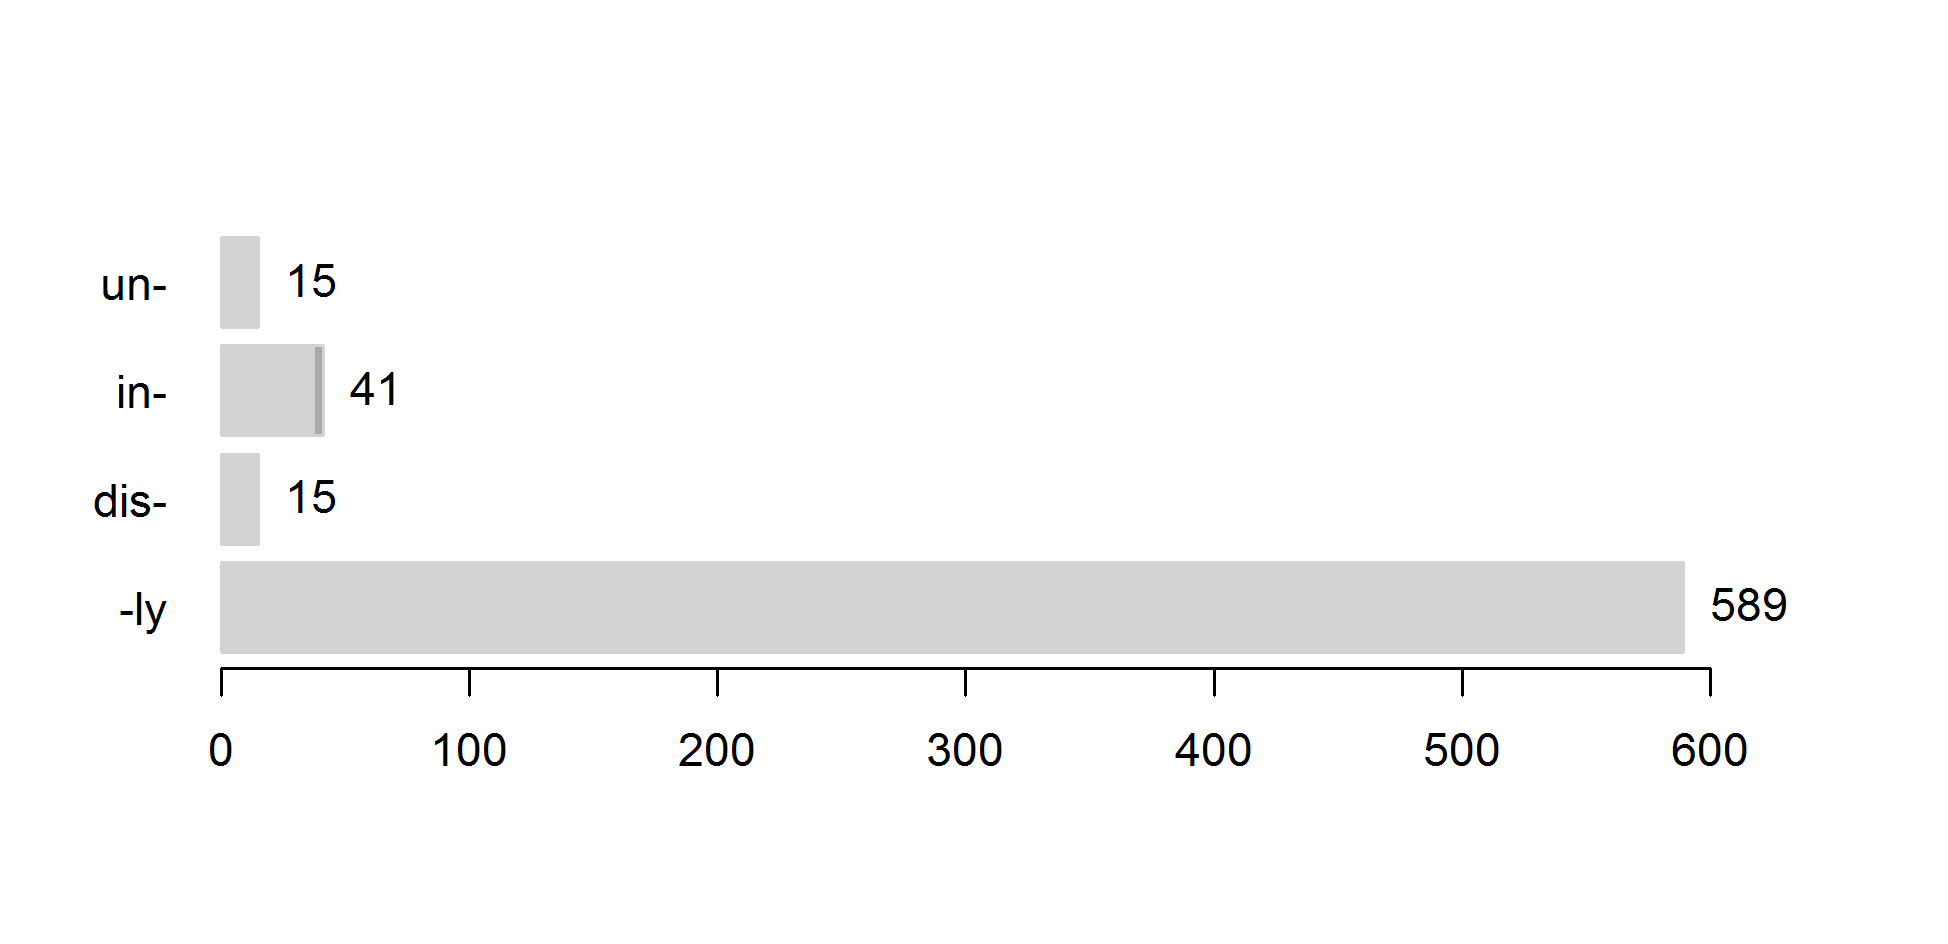
\includegraphics[scale=0.75]{images/Theory/NumberOfMorphGemAffixes.png}
	\caption{Number of types with morphological geminates for each affix\label{fig:morphological geminates for each affix}}
\end{figure*}

A comparison of the affixes reveals that while there are quite a lot of types with morphological \is{morphological gemination}geminates for the suffix \is{-ly}\suffix{ly}, the number of types is much smaller for all of the prefixes. In other words, there are not many \is{un-}\prefix{un}, \prefix{in} and \is{dis-}\prefix{dis}prefixed words with a {morphological geminate}. Especially the number of morphological \is{morphological gemination}geminates with \is{un-}\prefix{un} and \is{dis-}\prefix{dis} is very small and might raise methodological problems with regard to the investigation of some of the factors possibly influencing \isi{gemination}. Some variables, such as \is{frequency}frequencies, might not show enough variation to reliably be investigated. I will return to these issues in the pertinent sections of this book.

For the prefix \is{in-}\prefix{in}, the number of attested types with morphological \is{morphological gemination}geminates is much higher than for the prefixes \is{un-}\prefix{un} and \is{dis-}\prefix{dis}. However, out of the 105 attested types only one features the allomorph /ɪn/ (e.g. \textit{innumerable}). 33 types start with the allomorph\is{im-} /ɪm/ (e.g. \textit{immortal}), 51 with /ɪr/ (e.g. \textit{irregular}), and 20 with /ɪl/ (e.g. \textit{illogical}). 
This distribution has important consequences for the investigation of the prefix. Since the number of types in /ɪn/ is so limited, my investigation of \is{morphological gemination}gemination with \is{in-}\prefix{in} will mainly focus on the allomorph /ɪm/, for which more types exist. This is, as discussed in \sectref{previous empirical work}, in line with previous empirical work on \is{morphological gemination}gemination with \prefix{in}.
The investigation of /ɪr/  and /ɪl/ is not reasonable as derivatives with these allomorphs always feature a \is{morphological gemination}{morphological geminate}, i.e. there are no derivatives with /ɪr/  and /ɪl/ which feature a singleton consonant at their morphological boundary. This makes a comparison of the duration of a phonological double with a phonological singleton impossible.
   
%  \chapter {Morphological gemination: implications for theory} \label{Theory}

% Outlook of chapter
In this chapter, I will show how the gemination pattern of English affixes can shed light on various theories of the morpho-phonological and morpho-phonetic interface. I will discuss three different fields of theory which directly or indirectly predict the gemination pattern of English: Formal linguistic theories, psycholinguistic approaches of morphological processing and theories of speech production. After giving a general overview, I will discuss each field  separately, explain its main branches and deduce the predictions made for gemination with the five affixes investigated in this study.  At the end of the chapter, I will summarize the predictions of all theories discussed.\\


\section{Overview}
One can distinguish two major branches of morpho-phonological (or morpho-phonetic) theories. The first set of theories is formal, categorical and often generative in nature. Generally, in this type of theory it is assumed that phonological entities are abstract. Furthermore, these theories do not allow for a direct morpho-phonetic interface. Phonetic detail is thus believed to not mirror morphological structure directly. Depending on the theory, phonological rules and prosodic structure can, however, indirectly mirror the morphological structure of complex words and lead to phonetic effects. 
In these formal theories, morphological gemination is regarded as a categorical morpho-phonological and rule-based process, i.e. not as a gradient, word-specific process of the direct morpho-phonetic interface. Degemination is categorical and occurs when, due to some phonological rule or process, one segment of the double consonant is deleted. This deletion is then mirrored in phonetics. Depending on the theory, the predictions of which structures undergo degemination, and which structures display gemination, deviate. I will look at three prominent formal linguistic approaches in this book, i.e. Lexical Phonology, newer stratal approaches such as Stratal Optimality Theory, and Prosodic Phonology,  and discuss their predictions for gemination with the five affixes looked at in this study. 

% Second branch of theories#

The second branch of theories is psycholinguistic in nature and incorporates gradient, probabilistic factors. Experience-based effects, such as probabilities and frequencies of occurrence, play a major role in this type of theory. In contrast to formal approaches, theories of this kind do not assume gemination to be categorical and rule-based, but rather to be gradient and word-specific. In  general these psycholinguistic approaches assume a more direct relation between morphological structure and phonetics than formal theories by, for example, assuming that fine phonetic detail may be stored in the mental lexicon. In this study, I will concentrate on two prominent factors in psycholinguistic theory: decomposability and morphological informativeness. These two factors are believed to influence the phonetic realization of complex words, and should thus also play a prominent role in morphological gemination. 

% Distinction is not absolute

The binary classification of theories into formal, categorical approaches and gradient, probabilistic approaches must not be regarded as absolute. Formal linguistic theories may incorporate gradient, probabilistic factors, and in psycholinguistic approaches categorical concepts may be found. However, even though the categorization is not absolute, it helps to get a systematic overview of approaches which propose explanations for morpho-phonological and morpho-phonetic variation. The categorization simplifies the comparison of similar approaches, and helps with the identification of changes and developments of theories.

%Speech Production Theories
In addition to the two types of theories outlined above, I will also discuss speech production theories. There are various ways of how the morpho-phono-logical (or the morpho-phonetic) interface is modeled in speech production.  
I will present two different types of models. In the first type, a strict feed-forward structure with no explicit morpho-phonetic interface is assumed. The second type of model is based on exemplars, i.e. concrete mental entities which are formed from experience. While the former fits in better with the categorical approaches outlined above, the latter can be regarded to be more in the spirit of gradient approaches. 
However, I will desist from drawing explicit relations between speech production models and the different formal linguistic and psycholinguistic approaches discussed. The reason is that these relations are never explicitly mentioned in the literature, and that, due to the underspecification of morpho-phonological aspects in speech production models, a lot of information is not available that would be needed to relate the different theories with each other.
I will therefore review the two speech production models on their own. I will discuss them with respect to their understanding of morpho-phonological processes (such as, for example, morphological gemination), and will especially focus on the already mentioned underspecified aspects of the processing of complex words.  Because of these underspecifications no explicit predictions for gemination in English affixation will be drawn from these models. However, I will discuss more general assumptions the models make with regard to the phonetic realization of complex words. Some of these assumption can and will be tested in this study.



\section{Formal linguistic theories} 

In this section, I will discuss the following formal linguistic approaches: Lexical Phonology, newer stratal approaches such as Stratal Optimality Theory, and Prosodic Phonology. Within the framework of Prosodic Phonology, I will concentrate on the `prosodic word'.  In all three approaches morpho-phonological processes are assumed to be categorical in nature. Furthermore, in all of them affixes are believed to play a crucial role in morpho-phonological processes. The three approaches assume gemination to be a categorical process, i.e. either the two consonants of a morphological geminate remain and we find gemination, or one consonant is deleted and we find degemination. In all of the approaches boundary strength is one of the most important determiners for phonological behavior, i.e. also for gemination. 
One can thus see that there are quite a few similarities in the approaches. However, there are also important differences between them. One of these differences is the type of boundary assumed to be decisive for the phonological behavior of a derivative. While Lexical Phonology, for example, assumes affix-specific lexical differences in boundary strength, Prosodic Phonology defines boundary strength mainly in phonological terms. 
Another difference between the approaches is the assumed role of gradiency in morpho-phonological processes.
Crucially, these differences between approaches lead to different predictions for gemination. In the following, I will discuss each approach and present the predictions it makes for gemination with the five affixes investigated in this study.


\subsection{Lexical phonology} \label{LexPhon}


Lexical Phonology is one of the first theories which discussed the morpho-phono-logical interface and which makes clear predictions about gemination in English. According to Lexical Phonology (cf. \citealt{Kiparsky.1982,Mohanan.1986}), all morphological processes are carried out by modules in the lexicon. These modules are called levels or strata. A complex word is formed by retrieving entries from the lexicon which then undergo the morpho-phonological processes of the different strata. The strata are linked to specific affixes and are connected to phonological rules, which are carried out at the level they belong to. At each level one or more affixes can be added to a word. After affixation, the phonological rules adjust the form of the derivative so that the phonotactics of the language the word is formed in are met. During the word formation process an item can pass each level several times. A word does not leave a stratum until all operations the stratum holds for the word are carried out, i.e. all derivational or inflectional processes of a level are completed. This concept is called \newterm{cyclicity}. After a word has passed all strata, it leaves the lexicon and undergoes post-lexical rules. These rules adjust the word's sub-phonemic and word-external features. 
At the post-lexical stage the complex word does not carry any morphological information.  This is due to the principle of \newterm{bracket erasure}, which erases all morphological boundaries after each lexical level. Hence, according to Lexical Phonology the phonetics of a complex word does not show traces of its morphological structure.

Figure \ref{fig:Word Formation Process imperfectness} depicts the word formation process for the complex word \textit{imperfectness}, which consists of the level 1 prefix \prefix{in}, the root \textit{perfect} and the level 2 suffix \textit{-ness}.\footnote{Note that the figure only displays two levels, i.e. level 1 and level 2. These are the two levels relevant for affixation in English, i.e. the two levels relevant for this study. The number of assumed levels differs between different variants of Lexical Phonology (see \citealt{Giegerich.1999} for an overview), the level 1- level 2-distinction, as displayed in \figref{fig:Word Formation Process imperfectness}, is, however, agreed on by all variants.}
First, the root \textit{perfect} is retrieved from the lexicon and passed to the first level. After the level 1 affix \prefix{in} is added to the root, level 1 morphology passes the concatenated form to level 1 phonology, which applies the pertinent lexical rules. In this case, the adjacency of the two phonemes /n/ and /p/ triggers the application of an assimilation rule which changes /n/ to /m/. After this change in form, the word is passed back to level 1 morphology to check whether further affixes need to be added. Since this is not the case, the word leaves level 1 and is sent to the second level. 
Before entering level 2, all morphological boundaries of the derivative are erased (due to bracket erasure). When \textit{imperfect} undergoes level 2 processes it is thus treated the same way as a simplex word.  
In level 2, level 2 morphology adds the suffix \textit{-ness} to the derivative. The attachment of \textit{-ness} does not change the phonological form of the word, i.e. no phonological rules are applied. The derivative goes through level 2 morphology and phonology again to check whether additional morphemes need to be added. It then leaves the lexicon, i.e. it is passed to the post-lexical stage.\\

\begin{figure*} [t!]
	
	\centering
	\resizebox{.95\linewidth}{!}{%
	\begin{tikzpicture}[scale=0.7,every node/.style={scale=0.8}, framed]
	
	
	\node (LexicalEntries) [LexicalEntries] {Lexical entries};
	
	\node (MorphPhon1) [MorphPhon, below=2cm of LexicalEntries,  text width= 3 cm] {Morphology \textit{in + perfect imperfect}};
	\node (MorphPhon2) [MorphPhon, below=6cm of LexicalEntries,  text width= 3cm] {Morphology \\ \textit{imperfect + ness  imperfectness}};
	%	\node (MorphPhon3) [MorphPhon, below=10cm of LexicalEntries,  text width= 3 cm] {Morphology \textit{imperfectness}};
	\node (MorphPhon4) [MorphPhon, below=2cm of LexicalEntries,right =3cm of MorphPhon1,  text width= 6.7 cm ] {Phonology\\ \textit{in + perfect}   $\rightarrow$  /ɪmpɜɾfəkt/   \\  /ɪmpɜɾfəkt/ };
	\node (MorphPhon5) [MorphPhon, below=6cm of LexicalEntries,right =3cm of MorphPhon2,  text width= 6.7cm] {Phonology\\ \textit{imperfect + ness} $\rightarrow$  /ɪmpɜɾfəktnəs/ \\  /ɪmpɜɾfəktnəs/};
	%\node (MorphPhon6) [MorphPhon, below=10cm of LexicalEntries,right =3cm of MorphPhon3,  text width= 6.7cm ] {Phonology \\  /ɪmpɜɾfəktnəs/ };
	
	\node (PostLex) [PostLex, below=9.5cm of LexicalEntries, xshift=4.5cm  ] {Post-lexical rule application};
	
	
	% need to position the labels level
	
	\node (Level2) [Level, below=5.5 cm of LexicalEntries, xshift=4.5cm] {};
	%\node (Level3) [Level, below=9.5cm of LexicalEntries, xshift=4.5cm ] {};
	\node (Level1) [Level, below= 1.5 cm of LexicalEntries, xshift= 4.5 cm] {};
	
	\node (Level2caption) [below= 5.7  cm of LexicalEntries, xshift = -3cm] {Level 2};
	%\node (Level3caption) [below= 9.7  cm of LexicalEntries, xshift = -3cm] {Level 3};
	\node (Level1caption) [below= 1.7  cm of LexicalEntries, xshift = -3cm] {Level 1};
	
	
	\draw [arrowright] (LexicalEntries) -| node[midway,right, text width= 2 cm]{Retrieval of the root \textit{perfect}}(Level1);
	\draw [arrowright] (MorphPhon5) -- node [left, xshift=-1.5cm,  text width= 1.5 cm] {Bracket Erasure} (PostLex);
	
	%	\draw [arrowright] (MorphPhon6) -- node[left, xshift=-1.5cm,   text width= 1.5 cm] {Bracket Erasure} (PostLex);
	
	\draw [arrow2] (MorphPhon4.north west) --(MorphPhon1.north east);
	\draw [arrow2] (MorphPhon1.east) --(MorphPhon4.west);
	\draw [arrow2] (MorphPhon4.south west) --(MorphPhon1.south east);
	
	\draw [arrow2] (MorphPhon5.north west) --(MorphPhon2.north east);
	\draw [arrow2] (MorphPhon2.east) --(MorphPhon5.west);
	\draw [arrow2] (MorphPhon5.south west) --(MorphPhon2.south east);
	
	%	\draw [arrow2] (MorphPhon3) --(PostLex);
	
	\draw [arrowright] (MorphPhon4) -- node[left, xshift=-1.5cm,  text width= 1.5 cm] {Bracket Erasure} (MorphPhon2);	
	\end{tikzpicture}}
	\caption{Word formation process of \textit{imperfectness} in Lexical Phonology\label{fig:Word Formation Process imperfectness}}
\end{figure*}


As suggested by this example, level 1 affixes differ from level 2 affixes with regard to their boundary strength. The notion of boundary strength, as applied here, goes back to \cite{Chomsky.1968}. They assumed two different types of morphological boundaries: strong ones and weak ones.  While level 1 affixes trigger weak morphological boundaries, which go along with a high degree of phonological integration, level 2 affixes form strong boundaries and integrate less. The example \textit{imperfectness}  illustrates the difference. While the adding of the level 1 affix \prefix{in} leads to assimilation, neither the phonological  form of the base, nor the one of the suffix changes when the level 2 affix \textit{-ness} is added. One should, however, note that, even though the notion of boundary strength corresponds well with the theory of Lexical Phonology, \citet[239]{Kiparsky.1985} explicitly states that by introducing the different strata the notion of boundary strength becomes unnecessary in Lexical Phonology. 

Transferring the concept of lexical strata and its implications for the phonological relation between affix and base to gemination, the following picture emerges: a morphological geminate will degeminate when part of a level 1 affix, and it will geminate when part of a level 2 affix (see \citealt[18]{Mohanan.1986}). To find out what is predicted for the affixes under investigation, we need to determine which level each affix belongs to. 
Based on phonological and lexical properties, as well as on affix origin, Lexical Phonology assumes that the affixes \prefix{dis} and \prefix{in} belong to level 1, and that the affixes \prefix{un} and \suffix{ly} belong to level 2. Note that no differentiation between locative and negative \prefix{in} is made. Both belong to level 1.
Comparing the distinction between level 1 and level 2 affixes with the segmentability hierarchies proposed in the previous section, one can see that the distinction resembles the Non-Semantic Segmentability Hierarchy (\prefix{un} > \suffix{ly} > \{\prefix{dis}, \prefix{in}\textsubscript{\textsc{Neg}}\} >  \prefix{in}\textsubscript{\textsc{Loc}}). This hierarchy is based on lexical factors and ranks productivity and transparency above lexical meaning.  


Figure \ref{fig:LP predictions} depicts Lexical Phonology's prediction for gemination (and degemination) with the five affixes. Due to a morphological process a morphological geminate, i.e. a double consonant, emerges. For the level 1 affixes negative \prefix{in}, locative \prefix{in} and \prefix{dis} the theory predicts the deletion of one of the two adjacent consonants by some kind of phonological process. This deletion is expected to lead to a short duration of the morphological geminate, i.e. to degemination. For the affixes \prefix{un} and \suffix{ly} no deletion is expected, i.e. no phonological process is applied. The double consonant remains and the morphological geminate is therefore realized with a long duration. The affixes \prefix{un} and \suffix{ly} geminate.  
To summarize, according to Lexical Phonology, the level 2 affixes \prefix{un} and \suffix{ly} are expected to geminate, and the level 1 affixes negative \prefix{in}, locative \prefix{in} and \prefix{dis} are expected to degeminate. 

%\newpage
As described above, Lexical Phonology assumes gemination, i.e. the duration of the double consonant, to be mostly influenced by the type of affix involved. In other words, the affix involved affects consonant duration the most. However, there are additional factors which are assumed to also influence duration, namely post-lexical factors (e.g. speech rate, the preceding segment). Importantly, these factors are expected to be found on top of the expected effect of the affix. Lexical factors which mirror an individual word's morphological structure are not expected to play a role. All traces of morphological structure are erased by bracket erasure. 
The predictions of Lexical Phonology are summarized below \figref{fig:LP predictions}.



\begin{figure*} [h!]
	
	\centering
		\resizebox{.95\linewidth}{!}{%
	\begin{tikzpicture}[scale=0.8,every node/.style={scale=0.8}, framed]

	
	\node (Morph) [LingLevel,xshift=-8cm] {Morphologiocal Process};
	\node (Phono) [LingLevel, below=1 cm of Morph ] {Phonological Process};
	\node (Phone) [LingLevel, below= 1 cm of Phono] {Phonetic Realization};

	\node (MorphLev1) [LingLevel,right= 1.5cm of Morph] {\textit{in} + \textit{numerous} \\ \textit{in} + \textit{migrate}\\ \textit{dis} + \textit{satisfied}};
	\node (PhonoLev1) [LingLevel, right=1.5cm of Phono] {\textit{i}/n/\textit{umerous} \\ \textit{i}/m/\textit{igrate} \\ \textit{di}/s/\textit{atisfied}};
		
	\node (PhoneLev1) [LingLevel, right=1.5cm of Phone]{\textit{i}[n]\textit{umerous} \\ \textit{i}[m]\textit{igrate} \\ \textit{di}[s]\textit{atisfied}};

	\node (MorphLev2) [LingLevel,right=1.5 cm of MorphLev1] {\textit{un} + \textit{natural} \\ \textit{total} + \textit{ly}};
	\node (PhonoLev2) [LingLevel, right=1.5 cm of PhonoLev1] {\textit{u}/nn/\textit{atural} \\ \textit{tota}/ll/\textit{y}};
	\node (PhoneLev2) [LingLevel, right=1.5 cm of PhoneLev1]{\textit{u}[n:]\textit{atural} \\ \textit{tota}[l:]\textit{y}};
	
	\node(Level 1) [LingLevel, above= 1cm of MorphLev1]{\textbf{Level 1}};
	\node(Level 2) [LingLevel, above= 1cm of MorphLev2]{\textbf{Level 2}};
	
	\node(degemination) [LingLevel, below= 1cm of PhoneLev1]{\textbf{degemination}};
	\node(gemination) [LingLevel, below= 1cm of PhoneLev2]{\textbf{gemination}};	
	


	\draw [arrow4] (MorphLev1) --(PhonoLev1);
	\draw [arrow4] (PhonoLev1) --(PhoneLev1);
	\draw [arrow4] (PhoneLev1) --(degemination);
	\draw [arrow4] (MorphLev2) --(PhonoLev2);
	\draw [arrow4] (PhonoLev2) --(PhoneLev2);
	\draw [arrow4] (PhoneLev2) --(gemination);
		
	\end{tikzpicture}}
	\caption{Lexical Phonology: predictions for gemination with \prefix{un}, negative \prefix{in}, locative \prefix{in}, \prefix{dis} and \suffix{ly}}
	 \label{fig:LP predictions}
\end{figure*}




\newpage
\textbf{Lexical Phonology: Predictions}

\begin{enumerate}

	\item \prefix{un} geminates \\
	The nasal in \prefix{un}prefixed words with a phonological single consonant will be shorter than the nasal in \prefix{un}prefixed words with a phonological double consonant. %\\
	%-- \hspace{0.15cm} The /n/ in \textit{uneven} will be shorter than the /n/ in \textit{unnatural}.
	
	\item \prefix{in} degeminates \\
	The nasal in \prefix{in}prefixed words with a phonological single consonant will be as long as the nasal in  \prefix{in}prefixed words with a phonological double consonant.%\\ 
	%-- \hspace{0.15cm} The /n/ in \textit{inevident} will be of the same length as the /n/ in \textit{innumerous}. \\
	 %-- \hspace{0.15cm} The /m/ in \textit{implant} will be of the same length as the /n/ in \textit{immigrational}. 



	\item \prefix{dis} degeminates \\
	The fricative in \prefix{dis}prefixed words with a phonological single consonant will be as long as the fricative in \prefix{dis}prefixed words with a phonological double consonant. %\\ 
	%-- \hspace{0.15cm} The /s/ in \textit{disarm} will be of the same length as the /s/ in \textit{dissatisfy}. 
	

	
	\item \suffix{ly} geminates \\
	The lateral in \suffix{ly}-suffixed words with a phonological single consonant will be shorter than the lateral in \suffix{ly}-suffixed words with a phonological double consonant.%\vspace{0.15cm}\\ 
	%-- \hspace{0.15cm} The /l/ in \textit{truly} will shorter than the /l/ in \textit{really}. 
	
		\item Post-lexical factors affect consonant duration.
		
		\item Factors which mirror the morphological structure of individual words do not affect consonant duration.
	
\end{enumerate}



\subsection{Newer stratal approaches}

During the last decades various problems with Lexical Phonology have been revealed. These problems are closely related to the strict feed-forward structure of the model, as well as the strict division of labor between the strata (see also \citet[chapter 2]{Giegerich.1999} and \citet[chapter 7]{Plag.2003} for a thorough discussion). The criticism of Lexical Phonology has led to modifications of the theory and the development of newer stratal approaches, which are argued to solve the problems found with the original approach. Two of these approaches will be discussed in this section: the base-driven approach proposed by \cite{Giegerich.1999} and Stratal Optimality Theory. To understand the changes made in these newer approaches, it is necessary to take a closer look at the problems with the original approach.

One of the most prominent problems with Lexical Phonology is affix ordering. According to Lexical Phonology, level 1 affixes are attached to a base before level 2 affixes, and level 2 affixes are attached before inflectional affixes.\footnote{According to most varieties of lexical phonology (e.g.  \citealt{Kiparsky.1982,Mohanan.1986}) inflectional affixes belong to an additional stratum which follows derivation.} Therefore, level 2 affixes are not expected to be found within level 1 affixes, and inflectional affixes are not expected to be found within level 1 or level 2 affixes. However, in some derivatives these unexpected structures are found. For example, in the derivative \textit{interestingly} the inflectional suffix \suffix{ing} precedes the level 2 suffix \suffix{ly},\footnote{Note that this structure does not pose a problem to Lexical Phonology if \suffix{ly} is regarded as an inflectional suffix. However, Lexical Phonology adapts the view that \suffix{ly} is derivational. } and in the derivative \textit{ungrammaticality} the level 1 affix \suffix{ity} is attached before the level 2 affix \prefix{un}. Examples like these call into question whether the strict feed-forward structure proposed by Lexical Phonology is valid (see also \citet[chapter 4]{Plag.1999} for discussion).

Another problem with Lexical Phonology is the variation found within affixes. According to the theory, all affixes of one stratum, and thus all derivatives of one affix, should display the same (or at least very similar) behavior with regard to morpho-phonological processes. However, recent literature has pointed out that there is variation within the strata and even within the derivatives of one affix (cf., for example, \citealt{Raffelsiefen.1999,Bauer.2013, Plag.2014, BermudezOtero.2017}).  One prominent example of this variation is stress shift. The suffix \textit{-able}, for instance, is expected to preserve stress. There are, however derivatives with \suffix{able} in which stress shift is possible (e.g. \textit{ˈanalyze \textendash ˈanalyzable \textasciitilde anaˈlyzable}). With some derivatives stress shift even seems to  be consistent (e.g. \textit{ˈcategorize \textendash categoˈrizable}) (cf. \citealt[213 f.]{Plag.2014}). Empirical studies on stress confirm variation within affixes, i.e. different derivatives of the same affix deviate in their stress pattern (see for example \cite{Collie.2008} for \suffix{ion} and \suffix{ity}, \cite{Sanz.2017} for \suffix{ory}). The categorization of affixes as either level 1 or level 2 is insufficient to explain the variation found. 

A related, and maybe more essential, problem is the categorization of an affix as either level 1 or level 2. As summarized by \citet[134]{Raffelsiefen.1999}, level 1 affixes feature bound roots, are unproductive, determine stress, trigger assimilation and yield idiosyncratic meaning. Level 2 affixes attach to words, are productive, are stress-neutral, block assimilation and yield compositional meaning. However, as can be seen in \tabref{tbl:The affixes under investigation: a comparison} in \sectref{comparison affixes}, affixes often simultaneously feature level 1 and level 2 properties. Negative \prefix{in}, for example, assimilates, i.e. features a level 1 property, and is productive and semantically transparent, i.e. simultaneously features level 2 properties. This shows that the assignment of an affix to one or the other level is often not clear-cut. 

The three problems just discussed, i.e. affix ordering, intra-affix variation and the categorization of affixes, demonstrate that the strict division between level 1 and level 2 affixes, as well as the strict sequential order of level 1 and level 2 processes, are insufficient to explain the variation found in English derivatives. While this insufficiency has led some linguists to  abandon the idea of lexical strata in general (cf., for example, \citealt{Johnson.1997b,Bybee.2001,Pierrehumbert.2001,Hay.2001}), others have modified the stratal approach. 
\cite{Giegerich.1999}, for example, proposes a base-driven stratal approach. For English, he assumes two lexical strata: a root stratum and a word stratum. In the first stratum, i.e. the root stratum, all structure-changing morpho-phonological operations are carried out. In the second stratum, i.e. the word stratum, all structure-building processes take place. The important difference between Giegerich's approach and Lexical Phonology is that in Giegerich's approach, it is not the affix which is decisive for the stratum a derivative is formed in. Instead, the distinction between stratum 1 and stratum 2 is based on a derivative's base. If the base is a word, the derivative is formed in stratum 2. If the base is a root, the derivative is formed in stratum 1. In light of categorical approaches of morpho-phonology, degemination can be classified as a structure-changing process, i.e. a stratum 1 process. Thus, only derivatives featuring a root, i.e. stratum 1 derivatives, are expected to display degemination. Derivatives with words as their base are expected to geminate.

There are two major problems with Giegerich's approach  and the predictions it makes for gemination in English affixation. The first problem is that prefixation is not discussed, and that the approach is thus restricted to suffixation. One could assume that the predictions for suffixes can be extended to prefixes, i.e. one could predict prefixed words with words as bases to geminate and prefixed words with roots as bases to degeminate. It is, however, unclear whether this extension would comply with the approach. %Giegerich excluded prefixes from his theory on purpose and it is therefore questionable whether an extension to prefixes is acceptable. 
The second problem concerns the categorization of bases as roots or words. Giegerich does not give clear criteria for this categorization. This makes the testing of predictions for gemination which are based on the distinction of word vs. root, almost impossible. 
Furthermore, Giegerich states speaker-dependent differences, i.e. the same base might be a root for one speaker and a word for another (cf. \citealt[chapter 3.2.1.]{Giegerich.1999}). 
Due to these assumed differences among speakers, post-hoc explanations are available for all cases. If a word geminates, the speaker can be argued to have stored the base as a word. If a word degeminates, the opposite can be argued, i.e. the speaker has stored the base as a root. Because of these post-hoc explanations, the base-driven approach suggested by Giegerich might not be falsifiable. It is therefore not tested in this study.

Stratal Optimality Theory (`Stratal OT') is another, newer development of stratal approaches. It combines the modular feed-forward structure of Lexical Phonology with OT mechanisms (cf. \citealt{BermudezOtero.2012,BermudezOtero.2013,Kiparsky.2015,BermudezOtero.2017}). As in classical Lexical Phonology, the grammar is organized into three levels: two lexical levels and one post-lexical level. The first lexical level is the stem-level, the second is the word-level. The categorization of an affix as level 1 or 2 largely depends on the type of base it attaches to. If an affix attaches to a stem, it belongs to level 1, if it attaches to a word, it belongs to level 2 (cf. \citealt[7]{Kiparsky.2015}; \citealt[9 f.]{BermudezOtero.2017}).  Thus, as in Giegerich's approach, the base of a derivative plays a crucial role in Stratal OT. Also similar to Giegerich's approach, the categorization of a base as a stem or a word is not always clear. However, it can be assumed that all bound roots are classified as stems. Free-standing words might be classified as words. Crucially, in contrast to Giegerich's approach, speaker-dependent variation is not discussed in Stratal OT, i.e. post-hoc classifications are not an issue.

Stratal OT assumes each stratum to have its own constraint system. This system is responsible for phonological operations, i.e. also for degemination. As noted by \citet[5]{Kiparsky.2015}, the constraint system at each level consists solely of input/output and markedness constraints. No additional constraints are assumed. The order of constraints may deviate between the levels. For morphological geminates one can assume a different ranking of constraints at each of the two lexical levels. This difference leads to degemination on the stem-level and gemination on the word-level. It is thus assumed that level 1 affixes degeminate, while level 2 affixes geminate. This prediction is very similar to the prediction made by Lexical Phonology. There is, however, an important difference between the predictions of the two approaches. This difference is rooted in the assumption of dual-level affixes.

Different from classical stratal approaches, Stratal OT allows for dual-level affixes. According to Stratal OT, these affixes behave like level 1 affixes when attached to a stem and like level 2 affixes when attached to a word (cf. \citealt[15, 33]{BermudezOtero.2017}). 
\citet[33]{BermudezOtero.2017} notes the prefix \prefix{in} to be one of these affixes. He states that while in derivatives like \textit{importune} \prefix{in} behaves like a stem-level prefix, in derivatives like \textit{impolite} it behaves like a word-level prefix. The comparison of the five affixes investigated in this study revealed that the prefix \prefix{dis} behaves similarly to the prefix \prefix{in} (cf. \sectref{comparison affixes}). Like \prefix{in}, \prefix{dis} also features level 1 and level 2 properties, e.g. it attaches to words and to bound roots. It can therefore be claimed that \prefix{dis} also is a dual-level affix.  


%\enlargethispage{2\baselineskip}
Since the behavior of dual-level affixes depends on the type of base they attach to, variation in the gemination of \prefix{in} and \prefix{dis} is expected. The prefixes are expected to geminate when attached to a word. They are expected to degeminate when attached to a stem. As discussed above, the distinction between stem and word is, however, not always clear. In turn, the predictions are not always clear. However, for some words clear predictions can be formed. Since all bound roots are classified as stems, \prefix{in} and \prefix{dis} are expected to degeminate in all derivatives with a bound root. Only in derivatives with a word as a base \prefix{in} and \prefix{dis} can geminate.
The predictions for \prefix{un} and \suffix{ly} are very straightforward. According to Stratal OT, the two affixes belong to the second stratum. The prediction for \prefix{un} and \suffix{ly} therefore remains the same as in Lexical Phonology. Both affixes are expected to geminate.

\clearpage

Apart from dual-level affixes, there is another important difference between Lexical Phonology and Stratal OT.  This difference is related to the lexical storage of complex words. While according to Lexical Phonology all complex words are computed online, Stratal OT assumes stem-level derivatives to be stored as a whole (cf. \citealt[chapter 3]{BermudezOtero.2012}). Therefore, according to Stratal OT, frequency effects on level 1 derivatives are expected.  Words with a high frequency are expected to be reduced phonetically, i.e. should also display shorter durations of the affixational consonant. This reduction process is, however, not expected for level 2 derivatives wich are only stored analytically (cf. \citealt[chapter 3.3]{BermudezOtero.2012}). %Furthermore, bracket erasure is no longer assumed in Stratal OT, i.e. the morphological structure of complex words might influence the phonetic realization of a derivative.



One can summarize that while some of the basic assumptions of Lexical Phonology remained in newer approaches (e.g. modular feed-forward structure, lexical vs. post-lexical level), there are also some important differences (e.g. dual-level affixes, whole-word storage). These differences lead to different predictions for gemination with the five affixes of this study. While the prediction for the level 2 affixes \prefix{un} and \suffix{ly} remains the same, i.e. they are expected to geminate, variability is expected for the other two affixes. Another important difference to Lexical Phonology is that Stratal OT includes psycholinguistic, gradient factors, such as frequencies, by assuming whole-word storage of stem-level derivatives. Below the predictions of Stratal OT are summarized.\\


\textbf{Stratal Optimality Theory: Predictions}

\begin{enumerate}
	
	\item \prefix{un} geminates \\
	The nasal in \prefix{un}prefixed words with a phonological single consonant will be shorter than the nasal in  \prefix{un}prefixed words with a phonological double consonant. 
	%The /n/ in \textit{uneven} will be shorter than the /n/ in \textit{unnatural}.
		
	\item\prefix{in} degeminates in derivatives with a bound root\\
	 The nasal in \prefix{in}prefixed words with a phonological single consonant will be as long as the nasal in  \prefix{in}prefixed words with a phonological double consonant if  the derivative has a bound root as its base.
	%The /n/ in \textit{in} will be of the same length as the /n/ in \textit{inject}. \\
	%The /m/ in \textit{im} will be of the same length as the /n/ in \textit{im}. 

	\item \prefix{in} geminates in derivatives with a word as a base \\
	The nasal in \prefix{in}prefixed words with a phonological single consonant is shorter than the nasal in \prefix{in}prefixed words with a phonological double consonant if  the derivative has a word as its base.
	%The /n/ in \textit{inevident} will be shorter than the /n/ in \textit{innumerous}. \\
	%The /m/ in \textit{implant} will be shorter than the /n/ in \textit{immigrational}. 


\clearpage
	
	\item \prefix{dis} degeminates in derivatives with a bound root\\
	The fricative in \prefix{dis}prefixed words with a phonological single consonant will be as long as the fricative in \prefix{dis}prefixed words with a phonological double consonant if  the derivative has a bound root as its base.
	%The /s/ in \textit{dis} will be of the same length as the /s/ in \textit{diss}. 

	\item \prefix{dis} geminates in derivatives with a word as a base \\
	The fricative in \prefix{dis}prefixed words with a phonological single consonant is shorter than the fricative in \prefix{dis}prefixed words with a phonological double consonant if  the derivative has a word as its base.
	%The /s/ in \textit{disarm} will be shorter than s the /s/ in \textit{dissatisfy}. 

		
	\item  \suffix{ly} geminates \\
	The lateral in \suffix{ly}-suffixed words with a phonological single consonant will be shorter than the lateral in  \suffix{ly}-suffixed words with a phonological double consonant. 
	%The /l/ in \textit{truly} will shorter than the /l/ in \textit{really}. 
	
	\item Post-lexical factors affect consonant duration.
	


	\item Word frequency influences the duration of level 1 derivatives, i.e. \prefix{in} and \prefix{dis}prefixed words with a bound root.
	
\end{enumerate}



\subsection{The prosodic word} {\label{prosodic word}}


%Empirical work: morhological structure has indeed an effect on phonetis detail
Empirical work has shown that the morphological structure of a derivative may be directly mirrored in its acoustic realization. %(see for example \citealt{Sproat.1993b,Cho.2001,Sugahara.2009,Pluymaekers.2010,Schuppler.2012,Smith.2012,LeeKim.2013,Blazej.2015,Plag.2017}). 
\cite{Sproat.1993b}, for example, found differences in the phonetic realization of /l/ depending on the strength of the morphological boundary the sound occurred at. Stronger morphological boundaries were found to feature a darker and longer /l/ than weaker morphological boundaries. Similarly, \cite{LeeKim.2013} found that the phonetic realization of /l/ depends on the morphological structure of the derivative. 
For Dutch homophones, \cite{Schuppler.2012} found more reduction with complex words than with simplex words, i.e. word-final /t/ was more often deleted in simplex than in complex words.

With regard to duration, \cite{Cho.2001}, \cite{Sugahara.2009}, \cite{Hanique.2011}, \cite{Smith.2012} and \cite{Plag.2017} found systematic differences between monomorphemic and morphemic words with similar phonological structures. For Korean, \cite{Cho.2001} found articulatory evidence on the variability of intergestural timing in monomorphemic and complex words. In an EPG study, the timing of the gestures for [ti] and [ni] shows more variation when the sequence is heteromorphemic (i.e. across a morpheme-boundary) than when it is tautomorphemic (i.e. without straddling a boundary).
For English, \citet{Sugahara.2009} found phonetic differences between the final segments of a monomorphemic stem as against the final segments of the same stem if followed by a suffix. Stems followed by level 2 suffixes had slightly longer rhymes than their monomorphemic counterparts. \citet{Smith.2012} discovered systematic phonetic differences in the realization of the first three segments between prefixed words and what they call `pseudo-prefixed' words (such as \textit{mis-time} versus \textit{mistake}, respectively). Similarly \cite{Plag.2017} found a difference between morphemic and non-morphemic /s/ in English. They found non-morphemic /s/ to be longer than morphemic /s/. 


%no morpho-phonetic interface for stratal theories
The studies above raise the question of how to model the relation between morphology and phonetics. Even though the studies yield somehow contradicting results, i.e. in some of the studies stronger morphological boundaries lead to more reduction (e.g. \citealt{Sugahara.2009, Smith.2012}) and in some the opposite is the case (e.g. \citealt{Schuppler.2012, Plag.2017}), it seems certain that there is a stable effect of morphology on the acoustic realization of a word. One might thus suggest a morpho-phonetic interface which allows phonetics to directly access morphological information. This idea is picked up mainly by psycholinguistic approaches of morphological processing, which completely abandon the strictly feed-forward structure of stratal theory (cf. \sectref{Morphological Gemination: Implications for Psycholinguistic Theories of Morphological Processing}). 
In contrast, most formal theories hold on to the modular structure. These theories do not feature a direct interface between morphology and phonetics. Instead, they explain the effects of morphology on phonetics by referring to the prosodic structure of complex words (cf., for example, \citealt{Booij.1983b,Sproat.1993,Nespor.2007,Sugahara.2009,Bergmann.}). The prosodic structure of a derivative is closely connected to its morphological structure and is believed to directly influence the phonetic realization of a word. 

%Morphological boundaries are invisible to post-lexical stages of speech production, i.e. morphological structure is not directly accessible to phonetics. It follows that morphological boundary strength is not expected to be directly mirrored in fine phonetic detail. According to stratal theories, only categorical differences in boundary strength (, i.e. strong vs. weak boundary,) can be mirrored on the phonetic level. As discussed earlier in this section, differences in boundary strength between affixes lead to different degrees of phonological integration between base and affix, which in turn leads to different phonetic outcomes. Since differences in the phonetic realization between affixes are assumed to arise from categorical phonological operations, no gradient differences are expected. All gradient effects are attributed to post-lexical factors, i.e. non-morphological factors (cf. discussion of bracket erasure in this section).



% Prosodic boundaries
A very important concept in prosodic approaches, especially with regard to duration, is prosodic boundary strength. The common assumption is that the stronger the prosodic boundary, the less reduction is found. The strength of a boundary in prosodic terms highly depends on the prosodic domain it is adjacent to.
Figure \ref{fig:Prosodic Hierarchy} shows the prosodic hierarchy, which depicts the different prosodic domains.\footnote{Note that the constituents of the hierarchy differ slightly depending on author and approach. The hierarchy displayed here is taken from \citet[9]{Hall.2001}.} 
The higher the domain in the hierarchy, the stronger the boundary and the less reduction is expected. Segments followed by a intonational phrase boundary are, for example, expected to be less reduced than segments followed by a {phonological word} boundary.\footnote{The phonological word is also called prosodic word or p-word. In this book, I will use the terms interchangeably.}
 The effects of prosodic boundary strength are assumed to be additive, i.e. the more boundaries are present, the less reduction is expected. %With respect to gemination one could thus expect gemination with more and stronger prosodic boundaries and degemination with less and weaker prosodic boundaries.


\begin{figure*}
	\centering	
	
	\begin{tabularx}{.5\linewidth}{Y}
		phonological utterance (U)\\
						$\vline$	\\		
		intonational phrase (IP)\\
						$\vline$ \\
		phonological phrase	($\phi$)	\\
						$\vline$	\\		
		phonological word ($\omega$)\\
						$\vline$ \\
		foot 	(F)	\\	
						$\vline$ \\
		syllable ($\sigma$)	\\
	\end{tabularx}
	\caption{Prosodic Hierarchy}
	\label{fig:Prosodic Hierarchy} 
	
\end{figure*}					

% Phonological word: intro
Morphological geminates in English affixed words can occur at phonological word boundaries, foot boundaries and syllable boundaries. Since ``[t]he phonological word ($\omega$) represents the interaction between the phonological and the morphological components of the grammar'' (\citealt[109]{Nespor.2007}), the phonological word boundary is the most important for this study. In other words, gemination might be determined by phonological word boundaries, which mirror the morphological structure of a derivative and influence the acoustic realization of the complex word. The phonological word can be regarded as a mediator between the morphology and the phonetics of a complex word.

% garmmatical words and complex words
 A grammatical word can consist of one or more prosodic words (cf., for example, \citealt[29]{Booij.1983b}; \citealt[267]{Booij.1985}; \citealt[2]{Hall.2001}). Importantly, only complex words can consist of several prosodic words. This is due to the fact that prosodic word boundaries must align with morphosyntactic boundaries (see for example \citealt[2]{Hall.2001}). Crucially, not every morphological boundary corresponds to a p-word boundary. In other words, while some affixes form separate prosodic words, and thus occur at a p-word boundary, others form a prosodic word together with their base, i.e. are not adjacent to a p-word boundary. 
Examples of complex words with differing prosodic word structures are given below. The affixes in the words on the left constitute independent prosodic words. The affixes in the words on the right do not form independent p-words. They form one prosodic word together with their base. 

\begin{multicols}{2}

\begin{exe}
		\centering	
	\ex (\textit{un})\textsubscript{$\omega$}(\textit{natural})\textsubscript{$\omega$}, (\textit{un})\textsubscript{$\omega$}(\textit{told})\textsubscript{$\omega$}
\columnbreak
	\ex (\textit{really})\textsubscript{$\omega$}, (\textit{inject})\textsubscript{$\omega$}
\end{exe}

\end{multicols}



As stated by \citet[3]{Hall.2001}, prosodic words can form the domain of phonological and prosodic rules. It can thus be assumed that prosodic words also form the domain of gemination. While derivatives in which the affix forms a prosodic word on its own (e.g. (\textit{un})\textsubscript{$\omega$} (\textit{natural})\textsubscript{$\omega$}) geminate, affixes which form a prosodic word together with their base (e.g. \textit{(really)}\textsubscript{$\omega$}) degeminate (cf. \citealt[3543]{Giegerich.2012}; \citealt{Bergmann.}). In other words, reduction, i.e. degemination, is only found when the morphological geminate does not occur across a prosodic word boundary. The crucial question now is how to determine whether a morphological geminate occurs across such a boundary, i.e. whether an affix constitutes a prosodic word on its own.


% Sugahara and Turk for example show that  before suffixes of level 2 there is pqord boundary different from level 1 where there is non. Thus, for our affixes one could assume longer duration and gemination depending on their pword structure.


It is generally assumed that prosodic word structure corresponds to morphological boundary strength. Stronger morphological boundaries form phonological word boundaries. However, the specific criteria for determining prosodic words status are still debated in the literature (cf. \citealt{Raffelsiefen.1999}; \citealt{Hall.2001} for an overview).\footnote{Note that the criteria also deviate between languages. The overview given here is limited to the prosodic word in English.} 
In earlier approaches, prosodic word status was merely a mirror image of the level 1-level 2 distinction made in stratal theory. While level-1 affixes were assumed to be integrated in the p-word of their derivative, level 2 affixes were assumed to form a p-word on their own (see, for example, \citealt{Aronoff.1983,Booij.1983b,Szpyra.1989}). According to this view, the predictions for gemination made by Prosodic Phonology would be identical to the ones made by Lexical Phonology. Level 2 affixes form an independent p-word and thus geminate, level 1 affixes do not form an independent p-word and thus degeminate. 

More recent approaches to the prosodic word deviate from the stratal categorization. The prosodic word status of English suffixes, for example, is debated fairly often in the literature. The general assumption is that suffixes do not form prosodic words on their own (see, for example, \citealt[311]{Wennerstrom.1993}; \citealt[184]{Raffelsiefen.1999}; \citealt[401]{Hall.2001b}; \citealt{Sugahara.2009}). There are, however, different views with regard to the question of whether suffixes follow the prosodic word formed by their base (e.g. \textit{(run)\textsubscript{$\omega$}\suffix{ing}}), or whether they are integrated in the prosodic word of their base (e.g. \textit{(running)\textsubscript{$\omega$}}). While \cite{Sugahara.2009}, for example, suggest that all level 2 suffixes follow the p-word formed by their base, \cite{Raffelsiefen.1999} and \cite{Hall.2001b} propose that this is only true for some of those suffixes. They suggest that only consonant-initial suffixes, such as \suffix{ness} and \suffix{ly}, follow the prosodic word which is formed by their base. Vowel-initial suffixes, such as \suffix{ing} or \suffix{er}, are integrated in the prosodic word of their base. Examples of the p-word structures according to the two different approaches are given below. As can be seen, the suffix \suffix{ly}, which is under investigation in this study, is preceded by a p-word boundary in both approaches. It never is integrated in the p-word of its base.


\begin{multicols}{3}

	\begin{exe}
	
	\ex		
		\textbf{derivative}	\\
		\textit{run}\suffix{ing}	\\
		\textit{cool}\suffix{er} 	\\
		 \textit{cool}\suffix{ness}\\
		\textit{cool}\suffix{ly} \\			
		\columnbreak 
		
		\textbf{Raffelsiefen }	\\
		\textit{(running)\textsubscript{$\omega$}} 	\\
		\textit{(cooler)\textsubscript{$\omega$}} \\
		\textit{(cool)\textsubscript{$\omega$}\suffix{ness}} \\
		\textit{(cool)\textsubscript{$\omega$}\suffix{ly}} \\
		\columnbreak
			
		\textbf{Sugahara \& Turk}	\\
		\textit{(run)\textsubscript{$\omega$}\suffix{ing}} \\
		\textit{(cool)\textsubscript{$\omega$}\suffix{er}} 	\\	
		\textit{(cool)\textsubscript{$\omega$}\suffix{ness}}\\
		\textit{(cool)\textsubscript{$\omega$}\suffix{ly}}	\\

	\end{exe}
	
\end{multicols}

%\enlargethispage{\baselineskip}
%Wennerstr
Turning to the prosodic word status of English prefixes, two approaches are to discuss,  \cite{Wennerstrom.1993} and \cite{Raffelsiefen.1999}. \cite{Wennerstrom.1993} suggests the disinction between analyzable and non-analyzable prefixes. Prefixes which are analyzable form prosodic words, prefixes which are not analyzable do not. The key criterion for analyzability is focusability. If a prefix can be focused, it is analyzable and forms a prosodic word. 
Importantly, prosodic word status depends on individual derivatives and not on the prefix involved. This means that the same prefix might be considered a prosodic word in one derivative but not in another (\citealt[314]{Wennerstrom.1993}). 
As an example, \citet[311]{Wennerstrom.1993} presents the word \textit{external}, in which the prefix \prefix{ex} can be focused in a sentence such as ``\textit{The country has both INternal and EXternal problems}''. As shown in this example, analyzability is independent of whether the prefix's base is a bound root or a word. 

%Problems Wenners.
One problem with Wennerstrom's approach, as pointed out by \citet[161 f.]{Raffelsiefen.1999}, is that focusability does not correlate with phonological characteristics of p-words. Furthermore, it seems that almost every prefix can be focused under certain conditions (see also \citealt[chapter 4]{Plag.2003}). In normal, conversational speech there might be the additional problem of determining whether a prefix is focused or not. For these reasons focusability is not considered a useful, reliable criterion for determining prosodic word status.

%Raffelsiefen
\cite{Raffelsiefen.1999} proposes that segmentability correlates with prosodic word status. In more decomposable words, i.e. in derivatives in which the prefix is more segmentable, prefixes form independent prosodic words. In less decomposable words, they do not.
She suggests that morphological structure, i.e. decomposability, is `translated' into prosodic structure, which in turn is mirrored in the phonetic realization of a derivative. Derivatives made up of only one prosodic word, i.e. derivatives with less segmentable prefixes, are realized similarly to simplex words. The phonetic realization of prefixes which form prosodic words on their own, i.e. highly segmentable prefixes, is not affected by their base. 
A prefix's degree of segmentability in a given derivative is defined by the semantic and phonological properties of the derivative. 
Semantic and phonological aspects of segmentability are assumed to correlate with each other, an assumption which seems to be true for the affixes of this study (cf. \sectref{comparison affixes}). On top of decomposability, \citet[175 f.]{Raffelsiefen.1999} assumes an influence of frequency on prosodic word structure. %Very frequent words are less decomposable than complex words with lower frequencies. She also mentions that the decomposability of a word is mirrored in ther derivative's frequency in relation to the frequency of its base. Derivatives with a higher frequency than their base are less decomposable than complex words have a lower frequency than their base. \cite{Raffelsiefen.1999}
She suggests that derivatives of very high frequency are more likely to be parsed as a whole. In other words, high frequency derivatives are processed as single prosodic words irrespective of decomposability.


%With regard to perception, \cite{Raffelsiefen.1999} proposes that the phonetic realization of the derivative is used as a clue to parse the complex word. Words which show a high degree of integration of affix and base are parsed an one phonological word and are therefore accessed as a whole word. Words in which the affix is realized as a phonetically  independent unit are parsed as two prosodic words. The derivative is retrieved from the lexicon in its parts. 



\begin{table*}
	\caption{Criteria for prosodic word status of English prefixes (Raffelsiefen 1999)}
	\label{tbl:Criteria for prosodic work status of English prefixes (Raffelsiefen 1999)}
		\begin{tabular}{lll}
			\midrule
			\textbf{Criterion} & \textbf{Prosodic word }&\textbf{ No prosodic word }\\ 
								&\textbf{\textit{(prefix)\textsubscript{$\omega$}(base)\textsubscript{$\omega$}}}& \textbf{\textit{(prefix base)\textsubscript{$\omega$}}}
			\\
			\midrule 

			Stress & Secondary stress on prefix & Primary stress on prefix or  \\ 
							& 												& unstressed prefix \\
							&(e.g. \textit{ˌinˈtolerant, ˌdisˈhonor}) & (e.g. \textit{ ˈimpotent, inˈdifferent})
			\\ 
			
			Syllabification & No syllabification of  & Syllabification of  \\
						              &  prefixal coda 				& prefixal coda \\
						              & (e.g. \textit{dis.integrate})& (e.g. \textit{di.sease}) 
			\\ 
			
			Aspiration & Aspiration of 		& No aspiration of  \\
						       & base-intial stops &  base-intial stops \\
						       & (e.g. \textit{dis[k\textsuperscript{h}]olor}) & (e.g. \textit{dis[k]over})
			\\  
			
			%Glottalization & Glottalized stop in 	& No glottalized stop in \\
				%		              & prefix-final position & prefix-final position    
			%\\  
			
			Flapping & No flapping of  		& Flapping of\\
							 &  base-initial stop 	& base-initial stop\\
							& (e.g. \textit{in[t\textsuperscript{h}]olerant}) & (e.g. \textit{in[ɾ]egrate})
			\\   

			Type of derivative & Mostly of native origin & Mostly loanwords \\ 
			& (e.g. \textit{unpleasant, unjust}) & (e.g. \textit{inject, impotent})
			\\ 
						
			Meaning & Strictly compositional & Not compositional\\
							& (e.g. \textit{unpleasant, impolite}) & (e.g. \textit{inject, impotent})
			\\  
			
			Type of base & Word as a base & Bound root as a base\\
										& (e.g. \textit{unpleasant, impolite}) & (e.g. \textit{inject, innocent})
			\\ 
			

						\midrule
		\end{tabular}
\end{table*}

%\enlargethispage{\baselineskip}
To determine the segmentability of an affix, i.e. prosodic word status of a prefix, \cite{Raffelsiefen.1999} proposes a number of criteria. The criteria relevant for the prefixes under investigation are displayed in \tabref{tbl:Criteria for prosodic work status of English prefixes (Raffelsiefen 1999)}. Unfortunately, not all of the criteria turn out to be useful. Since prefixal stress is very hard to determine (especially in derivatives with base-initial primary stress) the stress-criterion is not suited to reliably determine prosodic word status (cf. \sectref{description un} for discussion of prefixal stress). Similarly, syllabification cannot always easily be determined and is thus not helpful. 
With regard to aspiration and flapping, these criteria are not applicable to all derivatives since they are restricted to specific sounds. In all derivatives with a double consonant a vowel follows the consonant, i.e. for none of these words the aspiration or the flapping criterion is applicable. Therefore, these two criteria cannot be used in this study.

The type-of-derivative-criterion merely displays a tendency and can therefore not be applied. 
This leaves us with two useful criteria: meaning and type of base. Prefixes which are semantically transparent and feature a word as a root are assumed to form independent prosodic words. Prefixes which are semantically opaque and feature a bound root are assumed to form prosodic words together with their base. 

There are two problems with the prosodic word approach and its predictions for gemination. 
The first problem is that the predictions made are restricted to certain combinations. No predictions are made for semantically opaque words with words as bases, or for semantically transparent words with bound roots. 
The second problem refers to the fact that only two criteria are applicable to determine prosodic word status, meaning and type of base. This is problematic because both criteria are lexical, i.e. not prosodic. Neither the meaning of a word nor its type of base can serve as direct evidence for a word's prosodic structure, and one must acknowledge the possibility that possible effects of the two factors on gemination are not due to prosodic word structure but to other lexical mechanisms. 
Nonetheless, it is justified to apply the two criteria `meaning' and `type of base' to test prosodic word status (as defined by Raffelsiefen). 

According to  \citeauthor{Raffelsiefen.1999}'s (1999) approach, meaning and type of base correlate with prosodic aspects of phonological word structure, e.g. stress and resyllabification. Therefore, these two lexical criteria can be applied to determine prosodic word status. 
One must, however, keep in mind that determining prosodic word status by applying lexical measures of decomposability is based on the prosodic word approach by \cite{Raffelsiefen.1999}, i.e. by the assumption of a close connection between prosodic and lexical word structure. There is the possibility that effects of meaning and type of base are independent from effects of prosodic structure. Prosodic criteria, such as syllabicity and stress, would be more direct determiners of phonological word structure. As described above, they are, however, not applicable, and further research on these prosodic criteria is needed to validly test phonological word status. 


\begin{table*}[b!]
	\caption{Prosodic word statuses of \prefix{un}, \prefix{in}, \prefix{dis} and \suffix{ly}}
	\label{tbl:Prosodic word statuses of affixes}
	\begin{center}
		\begin{tabular}{llll}
			\midrule
			\textbf{Affix }& \textbf{\textit{(base)\textsubscript{$\omega$} suffix}} \hspace{0.5 cm} & 
			\textbf{\textit{(prefix)\textsubscript{$\omega$}(base)\textsubscript{$\omega$}}} \hspace{0.5 cm}
			& \textbf{\textit{(prefix base)\textsubscript{$\omega$}}} \hspace{0.5 cm}
			\\
			\midrule 
			
			\prefix{un}&& \textit{(un)\textsubscript{$\omega$}(natural)\textsubscript{$\omega$}}&
			\\ 

			\prefix{in}& &{(im)\textsubscript{$\omega$}(polite)\textsubscript{$\omega$}} &\textit{(inject)\textsubscript{$\omega$}}
			\\ 

			\prefix{dis}& &{(dis)\textsubscript{$\omega$}(trust)\textsubscript{$\omega$}}&  \textit{(dissipate)\textsubscript{$\omega$}}
			\\  

			\suffix{ly}& \textit{(cool)\textsubscript{$\omega$} }\suffix{ly}	 & &
			\\   

			\midrule
		\end{tabular}
	\end{center}
\end{table*}

Table \ref{tbl:Prosodic word statuses of affixes} summarizes the analysis of the prosodic word status of  \prefix{un}, \prefix{in}, \prefix{dis} and \suffix{ly}. The predictions for gemination made by the prosodic word approach are based on this analysis. Affixes forming independent prosodic words are expected to geminate, affixes which do not form independent prosodic words are predicted to degeminate.
According to Raffelsiefen's approach, the three prefixes \prefix{un}, \prefix{in} and \prefix{dis} form prosodic words when they are part of a semantically transparent derivative with a word as a base. The prefixes are integrated in the prosodic word of their base when part of a semantically opaque derivative with a bound root. 
Note that, as discussed in \sectref{description un}, derivatives with \prefix{un} are always semantically transparent and feature words as a base. The prefix \prefix{un} is thus expected to always form a prosodic word and to always geminate. 
Gemination with \prefix{in} and \prefix{dis} is predicted to depend on the type of base the prefix takes in a given derivative. For semantically transparent derivatives with words as bases, gemination is predicted. For opaque derivatives with bound roots, degemination is predicted.
The suffix \suffix{ly} is always preceded by a prosodic word boundary, does, however, never form a prosodic word on its own. It is thus expected to degeminate. 
As noted above, \cite{Raffelsiefen.1999} additionally states that very frequent derivatives are parsed as a single prosodic word. Therefore, an effect of frequency on gemination is assumed. More frequent derivatives are more likely to degeminate. The predictions are summarized below.\\



\textbf{Prosodic Word (Raffelsiefen 1999): Predictions}

	
\begin{enumerate}

	\item \prefix{un} geminates \\
	The nasal in \prefix{un}prefixed words with a phonological single consonant will be shorter than the nasal in \prefix{un}prefixed words with a phonological double consonant. 
	%The /n/ in \textit{uneven} will be shorter than the /n/ in \textit{unnatural}.	
	
	\item\prefix{in} degeminates in semantically opaque derivatives with a bound root\\
	The nasal in \prefix{in}prefixed words with a phonological single consonant will be as long as the nasal in \prefix{in}prefixed words with a phonological double consonant if  the derivative is semantically opaque and has a bound root as its base.
	%The /n/ in \textit{in} will be of the same length as the /n/ in \textit{inject}. \\
	%The /m/ in \textit{im} will be of the same length as the /n/ in \textit{im}. 
	

	
	\item \prefix{in} geminates in semantically transparent derivatives with a word as a base \\
	The nasal in \prefix{in}prefixed words with a phonological single consonant will be shorter than the nasal in \prefix{in}prefixed words with a phonological double consonant if  the derivative is semantically transparent and has a word as its base.
	%The /n/ in \textit{inevident} will be shorter than the /n/ in \textit{innumerous}. \\
	%The /m/ in \textit{implant} will be shorter than the /n/ in \textit{immigrational}. 
	
	
	\item \prefix{dis} degeminates in semantically opaque derivatives with a bound root\\
	The fricative in \prefix{dis}prefixed words with a phonological single consonant will be as long as the fricative in \prefix{dis}prefixed words with a phonological double consonant if  the derivative is semantically opaque and has a bound root as its base.
	%The /s/ in \textit{dis} will be of the same length as the /s/ in \textit{diss}. 
	
	\item \prefix{dis} geminates in semantically transparent derivatives with a word as a base \\
	The fricative in \prefix{dis}prefixed words with a phonological single consonant will be shorter than the fricative in \prefix{dis}prefixed words with a phonological double consonant if  the derivative is semantically transparent and has a word as its base.\\
	%The /s/ in \textit{disarm} will be shorter than s the /s/ in \textit{dissatisfy}. 
	
	

	
	\item  \suffix{ly} geminates \\
	The lateral in \suffix{ly}-suffixed words with a phonological single consonant will be shorter than the lateral in \suffix{ly}-suffixed words with a phonological double consonant. 
	%The /l/ in \textit{truly} will shorter than the /l/ in \textit{really}. 
	
	\item Post-lexical factors affect consonant duration.
	
		\item Derivatives with higher token frequency will more likely degeminate.
	
\end{enumerate}






\section{Psycholinguistic approaches to morphological processing} \label{Morphological Gemination: Implications for Psycholinguistic Theories of Morphological Processing}

Empirical studies have found that the morphological structure of a derivative influences its acoustic realization, and that there thus is an effect of morphology on fine phonetic detail (see, for example, \citealt{Sproat.1993b, Cho.2001, Sugahara.2009, Pluymaekers.2010, Smith.2012, LeeKim.2013, Plag.2017}, see also discussion in \sectref{prosodic word}). 
In the previous section, this interaction between morphological and phonetic structure was explained by assuming a `mediator' between the two levels, i.e. the phonological word. However, there are certain restrictions connected with this assumption. Phonological word boundaries are restricted to mirroring categorical differences in morphological structure (for example simplex versus complex words, or weak versus strong boundaries). It follows that the prosodic word approach can only explain categorical, i.e. non-gradient, effects of morphological structure on phonetic detail. 
In contrast, some psycholinguistic approaches to morphological processing expect gradient, probabilistic effects of morphological structure on phonetic detail. In general, these approaches assume morphological structure to be gradient and to directly influence the phonetic realization of derivatives, i.e. they assume a direct morpho-phonetic interface. 

Different from formal linguistic theories, psycholinguistic approaches are main-ly based on empirical studies. On the one hand, these studies provide empirical support for the assumptions made by the approaches; on the other, differences in the studies' methodologies and outcomes preclude general, uniform theoretical assumptions about the morpho-phonetic interface. Assumptions and predictions are less formalized, less stream-lined and less precise than the ones of formal linguistic approaches. The predictions made are rather probabilistic, often revolve around one theoretical concept and often focus on the properties of individual words. 
 \cite{Hay.2001,Hay.2003}, for example, investigated the influence of decomposability on the phonetic realization of complex words.  She found more reduction with less decomposable derivatives than with more decomposable derivatives. 
\cite{Pluymaekers.2010} investigated the influence of an affix's informativeness on its phonetic realization and found that the more informative a linguistic unit is, the less phonetic reduction is found. 
\cite{Cohen.2014} conducted a study on the influence of an affix's paradigmatic probability on its duration. Her results showed that the more probable a suffix is, the shorter the preceding stem is pronounced.

In this study, I will focus on two frequently investigated and discussed concepts in psycholinguistic approaches: `decomposability' and `morphological informativeness'. Below I will lay out how and why they are assumed to influence the phonetic realization of affixed words. This discussion includes the discussion of models of word storage and morphological processing. Furthermore, I will provide an overview of previous empirical work.
 At the end of each section, I will present how each of the two factors is expected to influence gemination with \prefix{un}, \prefix{in}, \prefix{dis} and \suffix{ly}.

\subsection{Decomposability} \label{decomposability}

The idea that decomposability influences the phonetic realization of complex words is closely connected to dual-route models of morphological processing. These models assume that complex words are simultaneously stored as a whole and in their parts (cf., for example, \citealt{Frauenfelder.1992,Schreuder.2015,deVaan.2011,Caselli.2016}). According to these models, an affixed word like \textit{unnatural} has two separate entries in the mental lexicon, the whole-word form (\textit{unnatural}) and the decomposed form, which consists of two separate entries (\prefix{un} and \textit{natural}). Dual-route models stand in opposition to models which assume that a complex word is exclusively stored in its parts (cf., for example, \citealt{Prasada.1993,Marcus.1995,Clahsen.1999,Pinker.2002}). In these models, only irregular and non-transparent lexicalized forms are stored as a whole. Regular complex words, such as \textit{unnatural}, are always stored in their decomposed form and computed online. 

It is generally assumed that the way a word is accessed, i.e. as a whole or via computation, influences its phonetic realization. A word that is accessed as a whole will more likely show phonetic reduction than a word which is computed online.  This is due to the fact that in speech processing morphemes are recognized via their phonological segments, which in turn means that segments that represent morphemes should be more resistant to reduction. It follows that models that assume all complex words to be computed online, and all simplex words to be stored, predict systematic differences in the phonetic realization of complex and simplex words. Simplex words are expected to show more reduction. As discussed above, some empirical studies have indeed found the expected differences (see, for example, \citealt{Cho.2001,Sugahara.2009,Smith.2012}).
These purely computational models, i.e. the models predicting all complex words to be accessed via their parts,  do, however, not predict systematic differences between different complex words. Dual-route models in contrast predict these differences. Complex words accessed via the whole word route  are expected to be phonetically more reduced than complex words accessed via the decomposed route.



\cite{Hay.2001,Hay.2003} proposes that when accessing a complex word, both routes are activated. She argues that decomposability is the main factor governing  which route is faster in accessing the complex word. The assumption is that the more decomposable a complex word is, i.e. the more easily segmentable it is, the more likely it is accessed via its individual parts. The less decomposable a complex word is, i.e.  the less easily it is to segment, the more likely it is accessed as a whole. \cite{Hay.2001,Hay.2003} suggests `relative frequency' as the central measurement for decomposability. Relative frequency is defined as the frequency of a derivative relative to the frequency of its base. If a derivative is less frequent than its base, the derivative is rather decomposable and thus likely to be accessed via the decomposed route (e.g. \textit{impossible, softly}).  If a derivative is more frequent than its base, it is less decomposable and thus likely to be accessed as a whole (e.g. \textit{inject, swiftly}). 
The influence of relative frequency on the access route is explained by resting activations. A lexical entry of high frequency has a higher resting activation than an entry that is less frequently accessed. Higher resting activations lead to faster access, which in turn means that the route which is more frequently used will win the race when accessing a complex word. In other words, if the derivative is more frequent than its base, its resting activation is higher and the whole-word route is faster. If the base frequency is higher than the whole word frequency, the decomposed route has a higher resting activation and wins the race.


 
 
 \begin{figure*} [t!]
 	
 	\centering
 	\begin{tikzpicture}[scale=0.8,every node/.style={scale=0.8}]
 	
 	
 	\node (unnatural) [unnatural,  xshift=5.5cm] {\large{unnatural}};
 	
 	\node (derivative) [derivative, below=6cm of unnatural] {\large{\textit{unnatural}}};

 	\node (un) [un, below=2cm of unnatural, xshift=-5 cm] {\large{\prefix{un}}};

 	\node (natural) [natural, right=5.5cm of un] {\large{natural}};
 
  	\node (unsichtbar1) [derivative, above=1 cm of natural, xshift= 4 cm] {};
 	\node (unsichtbar2) [derivative, below=4 cm of unsichtbar1] {};
	
	
 	\draw [arrowN] (derivative) --(un);
 	 \draw [arrowN] (derivative) --(natural);
 	\draw [arrowN] (un) --(unnatural);
 	\draw [arrowN] (natural) --(unnatural);




	\draw [->, dashed, line width= 0.05 cm] (derivative)[out=20, in=60] ..controls(unsichtbar2) and (unsichtbar1).. (unnatural); 	

 	\end{tikzpicture}
 	
 	\caption{Dual-route model as in \cite{Hay.2001}} \label{fig:Dual-route model}
 \end{figure*}
 
Figure \ref{fig:Dual-route model} schematically depicts the race between the two access routes for the word \textit{unnatural}. The dashed arrow indicates the direct route and the solid arrows depict the decomposed route. The nodes represent the lexical entries for \textit{unnatural}, and the line width of a node indicates its activation level\footnote{Note that the activation level for the prefix \prefix{un} is not depicted in the picture. The role of the affix in the model will be discussed later in the chapter.}. A very frequent lexeme has a high resting activation (indicated by a thick line width). In our example, the frequency of \textit{natural} is much higher than the frequency of \textit{unnatural} (72.451 vs. 2.025 in COCA). This indicates that the resting activation of \textit{natural} is higher than the one of \textit{unnatural}. Therefore, it is assumed that the base \textit{natural} is accessed faster than the derivative \textit{unnatural}. In other words, the decomposed route is accessed faster than the whole word route. Note that the difference in frequencies, i.e. a much higher base frequency than derivative frequency, indicates that \textit{unnatural} is a highly decomposable derivative. We can can thus summarize that, according to the decomposability approach, the highly decomposable word \textit{unnatural} is predicted to be accessed via its parts and not via the whole word route.


As explained above, the route of access is assumed to be mirrored in the phonetic realization of a complex word. A word accessed via its parts is expected to display less reduction than a word accessed as a whole. Reduction is particularly expected at the morphological boundary. With regard to morphological gemination, a cross-boundary phenomenon, one can thus expect words which are less decomposable, and which are thus accessed as a whole, to be likely to degeminate, i.e. to show reduction. More decomposable words are expected to geminate, i.e. show no or less reduction. 
Turning back to the example above, one would thus expect gemination with \textit{unnatural}. Its high decomposability, and consequently the decomposed route via which it is accessed, suggests a low degree of reduction of the morphological geminate.


% empirical evidence
Empirical evidence for the effect of decomposability on the realization of complex words is contradictory and not conclusive. In the following, I will discuss six studies which investigated decomposability and found mixed results. The studies point at several complications with the approach. These complications have to be addressed in order to test the role of decomposability in morphological gemination, and in morphological processing in general. 

 \cite{Hay.2003} investigated  base-final /t/-reduction in \suffix{ly}-suffixed words. By comparing word pairs, she tested whether the stop is more reduced in less decomposable words than in more decomposable words. In the five word pairs she compared, one derivative was more decomposable than the other, i.e. one derivative was less frequent than its base (e.g. \textit{softly}) and one was more frequent than its base (e.g. \textit{swiftly}). The less decomposable words were expected to show more deletion and shorter durations.  \citeauthor{Hay.2003} found the expected effect. 
 However, as point-ed out by \cite{Hanique.2012}, \citeauthor{Hay.2003}'s methodology poses some problems. The number of investigated types is very small and hence hardly sufficient to draw general conclusions. Furthermore, instead of testing the direct effect of decomposability on duration, Hay compared average durations using a ranking system. This comparison does not allow for a straightforward interpretation. It is thus questionable how robust the effect found really is.

In {\citet{Hay.2007},  \prefix{un}prefixed words were investigated. It was tested whether more decomposable derivatives have a longer prefix duration than less decomposable  derivatives.  In contrast to \cite{Hay.2003}, this corpus study tested the influence of relative frequency on duration directly. The speech of two groups of speakers was investigated in the study: the speech of `early speakers', who were born before 1920, and the speech of `late speakers', who were born after 1920. 
While the expected effect of relative frequency on prefix duration was found for the early speakers, there was no effect  for the late speakers. Hay's explanation for the null result with late speakers is that those speakers use \prefix{un} less productively. Therefore, she claims, the prefix is less decomposable for late speakers in general. It is thus assumed that the segmentability of the prefix, which is not directly accounted for in relative frequency, interferes with the effect of relative frequency. In other words, the gradient measure of decomposability alone, i.e. relative frequency, might not be able capture a derivative's decomposability, and it might be necessary to also take an affix's average segmentability into account.
 
 \cite{Collie.2008} conducted a study on the effect of relative frequency on stress preservation with suffixes. While it was expected that derivatives which are accessed via the whole word route are less likely to maintain their prosodic structure, complex words accessed via the decomposed route were assumed to preserve their prosodic structure by demoting primary stress to secondary stress (e.g. \textit{acˈcelerate} \textendash  \textit{acˌceleˈration}). Derivatives which are more frequent than their base, i.e. derivatives of low decomposability, were thus expected to exhibit non-preserving behavior. While \cite{Collie.2008} found the expected effect for the suffix \suffix{ion}, the effect was not found for the suffix \suffix{ity}. This might mean that only some affixes are affected by gradient decomposability, i.e. relative frequency.
 	
 For Dutch, \cite{Hanique.2011} investigated the influence of relative frequency on the duration of schwa in prefix-final position. Three different prefixes (\prefix{ge}, \prefix{be} and \prefix{ver}) were investigated. Only for one of the three prefixes relative frequency showed a significant effect. For \prefix{ge} a higher relative frequency, i.e. a higher derivative frequency and a lower base frequency, led to shorter schwa durations.
 \cite{Hanique.2011} explain the differences in results between the prefixes by referring to differences in semantic opacity. While they analyze \prefix{ge} to be semantically transparent, the other two prefixes are analyzed as semantically opaque. It is suggested that relative frequency only affects transparent affixes since opaque derivatives are always  retrieved as a whole from the mental lexicon. Similar to \cite{Collie.2008}, this study thus reveals that not all affixes are affected by relative frequency and that categorical factors of decomposability, such as semantic transparency, might interfere with gradient effects of decomposability. 


That relative frequency does not have the same effect for all affixes is also shown by \cite{Schuppler.2012}. In their data set on Dutch complex words, derivatives with a higher relative frequency, i.e. a lower decomposability, show less word-final /t/-deletion than derivatives with a lower relative frequency, i.e. a higher decomposability. In other words, less reduction is found with less decomposable derivatives. This result goes counter the assumption that less decomposable words show more reduction. \cite{Schuppler.2012} explain their findings with reference to the informativeness of the affix, an idea further discussed in the next section.

The five studies mentioned above primarily concentrated on relative frequency as a measurement of a derivative's decomposability. The results reveal, however, that other measures of decomposability, i.e. semantic transparency (cf. \citealt{Hanique.2011}) and the productivity of the affix (cf. \citealt{Hay.2007}), might also be predictive for the realization of complex words.  
\cite{Burki.2011} investigated yet another measure of decomposability. They used a decomposability rating to predict schwa reduction in French complex words. Words rated as being less decomposable were expected to show more reduction. No effects were found. There are several possible explanations for the null result. 
The first (and most straightforward) explanation is that there is no effect of decomposability on schwa reduction. This explanation needs to be tested by further research. 
The second explanation is that a rating is not a suitable measure of decomposability. However, contra this explanation, \cite{Hay.2001,Hay.2003} showed that there is a significant correlation between decomposability ratings and relative frequency. If relative frequency is a suitable measure of decomposability, so should be decomposability ratings. It might, however, be the case that one of the two measures is a better predictor for durations in a particular type of model.  Differences in distributions and fine-grainedness of the measure might cause different effect sizes, as well as differences in significance between measures.   
The third explanation is also related to methodological aspects. In \cite{Burki.2011}, mean ratings were used and the authors explicitly mention the skewed distribution of the ratings, which, as just explained, might have influenced the results. Furthermore, only the ratings of five participants were included. This might have affected the validity of the rating in general. 
The question whether decomposability ratings are suitable to operationalize decomposability thus remains open at this point.


% summary results
The review of the empirical work on decomposability has revealed that the empirical facts are unclear and inconclusive. Some studies have found the expected effect of decomposability and some have not, one has even found the opposite effect (\citealt{Schuppler.2012}). 
One major reason for the incongruities between studies can be seen in their diverging methodologies. Two important issues, which are also relevant for the present investigation, have to be addressed  here. 
First, the studies investigated different phenomena in different domains (e.g. segment deletion in the base, affix duration, stress shift), and it might be that there are differences with regard to the influence of decomposability depending on the domain investigated. 
Second, the operationalization of decomposability varied across studies. This problem is also discussed by \citet[16]{Hanique.2012}, who state there is no uniform definition of decomposability and that ``[f]urther studies have to provide a better definition of morphological decomposability before we further investigate the role of morphological structure in speech production''. 
The most frequently used measure of decomposability is relative frequency, defined as the frequency of the derivative relative to its base. But even this seemingly well-defined measure was applied in different ways across studies. While some studies used it as a gradient measure (e.g. \citealt{Hanique.2011,Schuppler.2012}), in others it was used in categorical terms. \cite{Hay.2001} and \cite{Collie.2008}, for example, compared more decomposable with less decomposable words, i.e. instead of testing the gradient effect of relative frequency on phonetic realization, they redefined relative frequency as a binary measure. In addition to relative frequency,  the studies referred to semantic transparency (cf. \citealt{Schuppler.2012}), productivity (cf. \citealt{Hay.2007}) and a decomposability rating (cf. \citealt{Burki.2011}) as measures of decomposability. Furthermore, one can think of additional operationalizations of decomposability. \cite{Hay.2003}, for example, shows that phonological transparency correlates with relative frequency. Additionally, the type of base of a derivative or semantic similarity measures might be used.  

%affix specific
A second reason for differences in results might be related to the affix under investigation, as also suggested by some of the authors themselves (e.g. \citealt{Hanique.2011,Schuppler.2012}). It might be the case that only certain affixes are affected by certain decomposability measures (cf. \citealt{Collie.2008,Hanique.2011,Schuppler.2012}). It might, for example, be that only very productive, transparent affixes are affected by the a derivative's particular decomposability (as suggested by \citealt{Hanique.2011}). This idea is supported by \citeauthor{Hay.2007}'s (2007) data, in which prefix duration is only affected by relative frequency when the prefix is productive. The informativeness of an affix might also play a role, as suggested by \cite{Schuppler.2012} (see also next section fur further discussion). 
The idea that only transparent affixes are influenced by decomposability entails the assumption that only derivatives with transparent affixes can be accessed via the decomposed route,  i.e. that derivatives with opaque affixes will always be accessed as a whole. This in turn would mean that the predictions made by the decomposability approach are not only word-specific but must also concern the affixes involved.



%Thus prediction made by the approach not that easy to test
At first sight, the predictions made by the decomposability approach seemed quite clear: in complex words of high decomposability the morphological geminate will geminate, and in complex words of low decomposability the morphological geminate will degeminate. The discussion above has, however, shown that after all, the predictions are not that straightforward.
 How can one test the influence of decomposability, i.e. operationalize the concept? Which role does the affix play? Furthermore, one might raise the question of whether, according to the decomposability approach, degemination is predicted to be categorical or gradient. 

\clearpage


 To address the problem of how to operationalize decomposability, I will include five possible measures of decomposability in my studies: relative frequency, semantic transparency, type of base, a decomposability rating and semantic similarity scores. I will first investigate their relation to each other in order to validate their assumed correlation, i.e. ensure that they all tap into the same underlying concept. I will then test the predictions for gemination using the different measures. I will thus find out which variable is best suited to predict phonetic reduction in terms of duration.



Let us now turn to the role of the affix. In addition to investigating word-specific decomposability, I will also test affix-specific decomposability. There are two possible explanations of why we might find affix-specific effects. 
First, it might be the case that derivatives of one affix are so similar in their decomposability that practically all derivatives behave uniformly with regard to gemination. 
The second possibility is that, as suggested by previous research, only some of the affixes under investigation are affected by decomposability. To explore these possibilities, it is necessary to investigate the segmentability of the five affixes under investigation. 


\begin{figure*}[b!]
	\centering	
	

\begin{tabularx}{\linewidth}{lll}
	
	& \textbf{Segmentability}&	\textbf{Additional 	}  		  \\
	
	&	\textbf{hierarchy	}	&		\textbf{assumption }  	  \\		
	\midrule\\

		\textbf{Semantic} & \prefix{un} > \{\prefix{dis}, \prefix{in}\textsubscript{\textsc{Neg}}\}>  \prefix{in}\textsubscript{\textsc{Loc}} > \suffix{ly}& lexical meaning over pro-	 		  \\	
\textbf{Hierarchy}	& & ductivity, transparency and 	 		  \\	
& & type of base			 		  \\	
\\
\textbf{Non-Semantic}	&  	\prefix{un} > \suffix{ly} > \{\prefix{dis}, \prefix{in}\textsubscript{\textsc{Neg}}\}>  \prefix{in}\textsubscript{\textsc{Loc}}&		 productivity, transparency			   \\	
\textbf{Hierarchy}& & and  type of base	over   \\	
& & lexical meaning		  		  \\	
	\midrule \\						
\end{tabularx}

	
	\caption{Lexical segmentability hierarchies of  affixes}
	\label{fig:Lexical segmentability hierarchies of  affixes} 
	
\end{figure*}

 In \sectref{comparison affixes} we have already seen that there seem to be systematic differences in segmentability between the affixes. 
The two segmentability hierarchies which refer to lexical decomposability, i.e. the two hierarchies relevant for the decomposability approach, are depicted in \figref{fig:Lexical segmentability hierarchies of  affixes}. As discussed earlier, the two hierarchies deviate in the placing of the suffix \suffix{ly}, which is debatable and which depends on the role of semantics in decomposability \textendash  an issue which will be discussed further in the next section.
According to the decomposability approach, affixes which are more segmentable, i.e. affixes which are higher on the segmentability hierarchy, are expected to geminate. Affixes which are less segmentable, i.e. affixes which are lower on the hierarchy, are expected to degeminate. Furthermore, one might expect differences in the degree of gemination depending on the affix's position in the hierarchies. Gemination with more segmentable affixes is expected to be stronger than gemination with less segmentable affixes. The strength of gemination is expected to be mainly indicated by the durational differences between phonological doubles and phonological singletons. Stronger gemination goes together with larger singleton-double ratios.\footnote{Note that I will use the terms \newterm{strength of gemination} and \newterm{degree of gemination} interchangeably in this book. An affix which shows strong gemination, geminates to a high degree. An affix which shows weak gemination, geminates to a low degree.}




I will test the affix-specific decomposability predictions by first validating the segmentability status of the five affixes, i.e. I will look at the distributions of the different decomposability measures across affixes, and will thereby test whether the theoretically-based hierarchies are borne out by the data. I will then test whether there are significant differences in gemination behavior between affixes. If so, I will compare these differences with the segmentability hierarchies proposed. In other words, I will check whether  the differences in the degree of gemination between affixes mirror the differences in their segmentability.

% in which a phonological rule deletes one segment of the double consonant
Let us now turn the question of the nature of (de)gemination. The decomposability approach does not make clear predictions about the nature of degemination. Degemination can thus either be gradient, i.e. the double consonant shows more or less reduction, or categorical, i.e. in case of degemination there is no durational difference between singletons and doubles. %In contrast, the formal approaches discussed regard degemination as a categorical process in which one of the two double consonants is deleted by some kinf of phonological rule. 
If one assumes degemination to be categorical, one simultaneously assumes gemination to be governed by categorical factors. For certain categories, phonological doubles are categorically longer than phonological singletons. For others, there is no durational difference between doubles and singletons. 
If one assumes degemination to be gradient, one assumes gemination to be governed by gradient, word-specific factors.
%In this case, one would expect gradient durational differences between singletons and doubles which depend on word-specific factors.

In this study, I will explore both possibilities by investigating the distribution of durations across singletons and doubles, and by investigating which kind of factors govern gemination. %, i.e. categorical or word-specific factors. 
If gemination is categorical, the durations of singletons and doubles should show a bimodal distribution. Doubles should be longer than the singletons. If gemination is gradient, one would expect a gradient increase in duration from singletons to doubles, i.e. no binary distribution (cf.  \cite{Hanique.06.03.2013} for a similar analysis of distributions to investigate the nature of schwa reduction in Dutch). Furthermore, in case of gradient gemination, the durational difference between doubles and singletons should be affected by word-specific factors, such as, for example, relative frequency. In case of categorical gemination, the durational difference between doubles and singletons should be affected by categorical factors, such as, for example, the affix.
 


%\newpage
%\enlargethispage{\baselineskip}
To summarize, one can state that up to this point the decomposability approach does not make clear, spelled-out predictions for gemination. Before testing the effect of decomposability on gemination, it is necessary to explore the concept of decomposability with its possible operationalizations and domains. Also, the approach does not make assumptions about the nature of gemination, i.e. it is yet to explore whether gemination is gradient or categorical. 
For these reasons the predictions uttered at this point remain relatively vague. 

Two different predictions with regard to the effect of decomposability are formulated. One concerns the decomposability of the individual derivative, and one the segmentability of the affix. They will be tested using different decomposability measures. i.e.  relative frequency, semantic transparency, type of base, a decomposability rating and semantic similarity scores. The two predictions are spelled out below.\\


\noindent \textbf{Morphological Segmentability Hypothesis: Predictions}
\vspace{0.45 cm}	

\noindent	\textbf{A:\hspace{0.5cm}The decomposability of an individual word influences gemination} \vspace{0.2 cm}
   
\noindent  The more decomposable a derivative is, the higher is its degree of gemination. \\

\noindent The less decomposable a derivative is, the lower is its degree of gemination. \\


	



\noindent	\textbf{B: \hspace{0.5cm}The segmentability of an affix influences gemination} \vspace{0.2 cm}
	
	
\noindent	The more segmentable an affix is, the higher is the degree of gemination with words containing that affix. \vspace{0.2cm}
	
\noindent		The less segmentable an affix is, the lower is the degree of gemination with words 
		containing that affix. \\
		
		\vspace*{0.3cm}

In addition to the two decomposability predictions, two predictions with regard to the nature of gemination are formulated. One predicts gemination to be categorical, the other predicts gemination to be gradient. They will be tested by investigating the distribution of durations in the data sets and by investigating the type of effects governing gemination. Note that the two predictions concerning the nature of gemination are not exclusive to the decomposability approach but concern all approaches discussed. While formal approaches explicitly predict gemination to be categorical, the psycholinguistic approaches leave the question open. The two predictions are displayed below.\\


\noindent \textbf{Nature of gemination: Predictions}\\	\label{predictions nature of gemination}

\noindent \textbf{A:\hspace{0.5cm}Gemination is categorical} \\



\noindent	The duration of the affixational consonant(s) in the data set shows a bimodal distribution with one mode representing doubles and one mode being singletons.
	
\noindent	Doubles are longer than singletons. 
	
\noindent	Gemination is governed by categorical factors.	\\



\noindent	\textbf{B: \hspace{0.5cm}Gemination is gradient} \\
		
\noindent	The duration of the affixational consonant(s) in the data set does not show a bimodal distribution with one mode representing doubles and one mode being singletons. 

\noindent	The duration of the affixational consonant(s) increases gradually from singletons to doubles.  
	
\noindent	Gemination is governed by word-specific factors.
	



\subsection{Morphological informativeness} \label{morphological informativeness}

The idea that linguistic units with high information load are less prone to phonetic reduction than linguistic units with low information load is well established in psycholinguistic approaches  (cf., for example, \citealt{Aylett.2004,Kuperman.2007,Pluymaekers.2010,Hanique.2012}). Following \cite{Lindblom.1990}, in speech production two forces work against each other: economy of articulatory effort and discriminability of the speech signal. On the one hand, speakers want to put as little effort as possible in producing speech, on the other, they want to ensure the intelligibility of the speech signal. As a result, they only put as much effort in pronunciation as they estimate to be necessary for the listener to discriminate the speech signal. A speaker's amount of effort is mirrored in the degree of reduction found in the speech signal, and depends on the information load of the linguistic unit. The degree of information load in turn is influenced by various factors, such as probability of occurrence, semantic information load and redundancy (see also \cite{Kuperman.2007} for discussion).  
Elements with low information load, i.e. redundant elements with higher probabilities of occurrence and less semantic information load, are realized with less effort and are hence more reduced than elements with higher information load. They are shorter and less salient. 

The elements under investigation in this study are affixes. Following the approach just described, one can assume affixes with higher information load to show less reduction than affixes with lower information load. Degemination can be defined as some sort of reduction. Even though the nature of gemination is yet unclear (see \sectref{decomposability} for discussion on gradient vs. categorical gemination), it is certain that degemination results in some kind of phonetic reduction. It is thus predicted that affixes with higher information load are less prone to degemination than affixes with lower information load, and that the degree of (de)gemination depends on the degree informativeness of the affix.

To test this prediction, it is necessary to measure the information load of the affixes.
 In this study, the predictability of the affix and the semantic information load of the affix are used as indicators of informativeness.
The predictability of an affix is closely related to its probability of occurrence. 
 If an affix is probable to occur, it is very predictable and thus not very informative. %In turn, reduction is likely. 

 
 Probability can be operationalized in various ways. 
   %Paradigmatic Probability
   \cite{Pluymaekers.2010}, for example, tested the effect paradigmatic probability on duration to investigate the effect of informativeness on phonetic reduction.
 They investigated Dutch \textit{-igheid} (/əxhɛit/), which represents three different morphological structures. In some words \suffix{igheid} represents one single suffix (`\textit{-igheid}-words'), in some \suffix{ig} belongs to the base word and only \suffix{heid} is the suffix (`\textit{-heid}-words'), and for some words both parsings are possible (`\textit{ambiguous} words'). \cite{Pluymaekers.2010} measured the informativeness of the investigated structures by counting the cohort of competitors in the morphological paradigm for each structure. 
 The more competitor words in a paradigm, the less probable, and thus the more informative, the structure is.  Since the paradigm for \suffix{heid}-words is the least dense, i.e. this suffix has the least competitors, it is the least informative and most reduction is expected with words of this kind. Reduction was measured in terms of the duration of the /xh/ cluster. \cite{Pluymaekers.2010} found the expected effect. The structure with least competitors in the morphological paradigm, i.e. the least informative structure, showed most reduction.
  
  
 Similarly \cite{Schuppler.2012} found a relation between informativeness in terms of number of competitors in the morphological paradigm and reduction. 
 As laid out in the previous section, in their data complex words with a low relative frequency, i.e. highly decomposable words, showed more base-final /t/ reduction than less decomposable words. This goes against the assumptions made by the decomposability approach, and is the opposite of what was found for English adverbial \suffix{ly} in \cite{Hay.2003}. 
 
 \cite{Schuppler.2012} explain the difference between their and Hay's results by referring to differences in informativeness between the two investigated structures. 
 They hypothesize that relative frequency might play a different role for suffixes with higher information load, i.e. less probable suffixes, than for suffixes with lower information load. According to \cite{Schuppler.2012}, English \suffix{ly} is more probable and less informative than the Dutch suffix \suffix{t}. 
 English adverbs always end in the suffix \suffix{ly}, i.e. it has a high paradigmatic probability. The suffix is thus expected and does not feature a high information load. It differs in this respect from the inflectional Dutch suffix \suffix{t}, which is only one of three possible forms in the inflectional paradigm. According to \cite{Schuppler.2012}, the suffix \suffix{t} is therefore generally less probable than \suffix{ly}. It has a higher information load and is not reduced. In other words, because Dutch inflectional \suffix{t} is very informative, lower decomposability does not lead to more reduction with this affix. Lower decomposability leads to more reduction with the less informative English adverbial suffix  \suffix{ly}.
 
 
 %Why I don't use it 
The two studies above suggest that paradigmatic probabilities might be a good measure of predictability. However, this measure is not applicable in this study. The reason is that it is yet unclear how to measure the paradigmatic probability of derivational prefixes. 
 To nevertheless investigate the predictability of the affixes in this study, 
another type of probability was looked at: syntagmatic probability. 

As shown in \cite{Hanique.06.03.2013}, syntagmatic probability can also successfully be used as an indicator of predictability and informativeness. In \cite{Hanique.06.03.2013}, the deletion of word-final /t/ in Dutch past participles and in Dutch simplex words was investigated.  The segment was more often deleted in complex than in simplex forms. 
  \cite{Hanique.2012}  argue that the results can best be accounted for by reference to the informativeness of the suffix \suffix{t} in comparison to the informativeness of the segment /t/ in corresponding simplex structures. Since most Dutch participles end in /t/, the segment is highly predictable in complex words. Therefore, it is less informative than /t/ in corresponding simplex words. The higher reduction rate of /t/ in complex words can thus be explained by the low degree of informativeness of the suffix \suffix{t}.
  
  
Let us now turn to the affixes under investigation in this study. Out of the five investigated affixes, the suffix \suffix{ly} features the highest syntagmatic probability. Due to its function to create adverbs, its syntagmatic probability is very high, and, in turn, its predictability is very high. As the prefixes are not associated with a specific function, they are much less predictable.  
Furthermore, the suffix \suffix{ly} is more predictable than the prefixes because of its position at the end of the word. 
 Prefixes precede their base, which means that the base of prefixes does not serve as a cue for the occurrence of the prefix. Prefixes can basically occur after any word after which its base can occur. 
 For example, the prefix \prefix{un} as in \textit{uncool} can occur after any word after which the word \textit{cool} can occur. 
 In contrast, suffixes follow their base. Their occurrence is restricted by the amount of base words they can take,  and their base serves as a cue for their occurrence.
 It follows that the syntagmatic probability of prefixes, and in turn their predictability, is generally lower than the one of suffixes. 
 
Overall, the discussion of predictability has shown that the suffix \suffix{ly} is the most predictable affix in this study. It is much more predictable than the prefixes in this study. The differences in predictability between the prefixes is less clear. As explained above, paradigmatic probabilities are not useful in order to measure a prefix's predictability. Furthermore, it seems quite challenging to assess differences in the syntagmatic probability of derivational prefixes. As prefixes occur before their base, and as they are not associated with a specific function, it is unclear on which base one can compare their probability of occurrence.




%Semantic Information Load

In addition to predictability, the semantic information load of an affix can also serve as a measure of its informativeness. An affix that contributes more to the meaning of a derivative is more informative than an affix which does not feature clear semantic content. Semantic information load is particularly interesting as a measure of informativeness for derivational prefixes (as the ones in this study), for which the application of other informativeness measures is quite problematic. 

The semantics of the affixes under investigation were discussed thoroughly in \sectref{comparison affixes}. While some affixes, such as \prefix{un}, feature a stable, transparent meaning, others, like locative \prefix{in} and \suffix{ly}, do not. The Semantic Segmentability Hierarchy in \figref{fig:Lexical segmentability hierarchies of  affixes} depicts the decline in semantic information load of the five investigated affixes.
 The lower the affix is positioned on the hierarchy, the less semantic information it conveys, and the less informative it is. The hierarchy shows that the suffix \suffix{ly} is the least informative affix with regard to its semantic information load.  As discussed earlier, the suffix does not contribute any lexical meaning to the derivative. 
 For the prefixes, \prefix{un} is the prefix with the most transparent and stable meaning, i.e. the affix with the highest information load. Negative \prefix{in} and \prefix{dis} denote a stable, negative meaning in most derivatives but there are also some derivatives in which the affix does not contribute a clear lexical meaning. Locative \prefix{in} features the least semantic information of the prefixes (see \sectref{affixes} for detailed discussion of the semantics of all five affixes). 

One can summarize that, due to its high predictability and low degree of semantic contribution to a derivative's meaning, the suffix \suffix{ly} is the least informative affix in this study. It is thus expected to show the weakest degree of gemination. 
The analysis of the prefixes' informativeness is mainly based on semantic factors. 
The analysis revealed that \prefix{un} is the most informative prefix. It is thus expected to show the highest degree of gemination. 
The informativeness of locative \prefix{in}, negative \prefix{in} and \prefix{dis} is less clear and might vary among types. In derivatives with transparent meaning, the affixes are more informative than in derivatives with opaque meaning. This means there are two possible predictions for the gemination with these three prefixes: an affix-specific one and a word-specific one. 

According to the affix-specific prediction, one would predict the overall informativeness of the affix to govern gemination. This means one would predict gemination to pattern according to the Semantic Segmentability Hierarchy. While gemination with \prefix{un} is expected to be the strongest, and gemination with \suffix{ly} is expected to be the weakest, the other three prefixes are expected to pattern in between. Importantly, one would not predict word-specific effects according to this prediction. 

According to the word-specific prediction, one would predict informativeness to be word-specific, i.e. in semantically transparent words a prefix is more informative than in semantically opaque words. Since \prefix{un} is always semantically transparent, it is predicted to always display a high degree of gemination. For the other three prefixes the degree of gemination is expected to depend on semantic transparency. Opaque derivatives should display weaker gemination than transparent derivatives. 

In this study, I will test both predictions made by the morphological informativeness approach, i.e. the affix-specific and the word-specific prediction. The predictions are summarized below.\\


\noindent \textbf{Morphological Informativeness: Predictions}\\	

\noindent 	\textbf{A:\hspace{0.5cm} Affix-specific informativeness influences gemination}\vspace{0.2 cm}
	
\noindent		The more informative an affix is, the higher is the degree of gemination with words containing that affix. \\
		
\noindent	The less informative an affix is, the lower is the degree of gemination with words 
		containing that affix. 
	
				\begin{itemize}
	\item	Gemination patterns according to the Semantic Segmentability Hierarchy. 		\\
		

\end{itemize}


	
\noindent	\textbf{B: \hspace{0.5cm} Word-specific informativeness influences gemination}\vspace{0.2 cm}
	
\noindent	The more informative an affix is in a given derivative, the higher is the degree of gemination in the derivative.\\ 


	
\noindent	The less informative an affix is in a given derivative, the lower is the degree of gemination in the derivative.% words
	
			\begin{itemize}
				
				\item Derivatives with the prefix \prefix{un} geminate to a high degree.		
				\item Derivatives with the suffix \suffix{ly} geminate to the lowest degree.
				\item  Derivatives with transparent semantics and the prefixes \prefix{dis}, negative \prefix{in} and locative \prefix{in} geminate to a high degree.	
				\item  Derivatives with opaque semantics and the prefixes \prefix{dis}, negative \prefix{in} and locative \prefix{in} geminate to a low degree.	\\
			\end{itemize}	



 
\section{Speech production models}\label{speech production models}
%\enlargethispage{\baselineskip}

Speech production models are closely connected to the approaches discussed in the previous sections. As formal linguistic and psycholinguistic approaches, they also make assumptions about the morpho-phonological interface and are thus relevant for this work. However, speech production models are broader than the approaches previously discussed in that they are not solely concerned with the morpho-phonological interface but with speech production as a whole. In other words, the morpho-phonological interface, and the processing of complex words, form just a small part of these models.

 Two types of  speech production models can be distinguished: modular feed-forward models (cf. \citealt{Levelt.1999,Levelt.1999b,Levelt.2000}) and usage-based models (cf. \citealt{Johnson.1997b,Bybee.2002,Pierrehumbert.2001,Pierrehumbert.2002}). With regard to morphological processing, the two types differ in their assumptions of how words are stored, as well as which factors influence the phonetic realization of morphemes. Crucially, neither is very explicit with regard to the morpho-phonological interface and no specific claims about the interplay of phonetics and morphology are made. Therefore, no explicit predictions about gemination can be drawn from the models. The data in this study might nevertheless provide evidence for the theoretical modeling of  speech production by displaying general effects on duration. By investigating which morphological factors influence segmental duration at morpheme boundaries, general assumptions about the morpho-phonological interface made by different types of speech production models can be tested.

In traditional speech production models, such as  \cite{Levelt.1999b}, two main stages of processing can be distinguished: the lexical stage and the post-lexical stage. At the lexical stage lemmas are retrieved and grammatically encoded. At the post-lexical stage the morpho-phonological and the phonetic encoding take place, i.e. the relation of morphological and phonetic structure is defined at this stage. After all morphemes of a lemma are activated and assembled, their morpho-phonological code is spelled out. This code is segmental in nature. The spelled-out segments are then syllabified to form `phonological words'.\footnote{Note that the term `phonological word' in \cite{Levelt.1999b} is not synonymous with the term in the prosodic word approach (cf. \sectref{prosodic word}). } In a last step utterance prosody is generated to compute the `phonological score', which serves as the basis for articulation. In other words, the phonological score is translated into phonetics, which is in turn translated into concrete instructions for the articulators (`articulatory score').

%\newpage
The crucial point with regard to morpho-phonological processing is that articulation is based on phonemic representations, i.e. the segmental morpho-phono-logical code. The question is whether morphological structure is present at this stage, and if so, how it is mirrored in the acoustic realization of complex words.
 As discussed by \citet[1037]{CohenGoldberg.2013}, most traditional models, such as the one just described or the one suggested by \cite{Dell.1986}, are largely silent about the post-lexical processing of multi-morphemic words. It is simply not stated whether the assembly of morphemes leaves traces in the phonological make-up of a word. However, since none of the models mentions any process which suggests that morphological structure is preserved in morpho-phonological encoding, it can be assumed that phonemic representations do not feature any traces of morphological structure. This also means that, according to traditional models of speech production, there is no difference in the phonemic representation of morphologically complex and morphologically simplex words, i.e. there is no difference in their acoustic realization.

Recent studies have challenged this assumption by showing that phonemically identical strings of different morphological status vary systematically in their phonetic realization. For example, \cite{Kemps.2005} and \citet{Blazej.2015} found that phonologically identical free and bound variants of a base (e.g. \textit{clue} without a suffix compared to \textit{clue} in \textit{clueless}) differ acoustically.
As already discussed in \sectref{prosodic word}, other studies demonstrate that the realization of segments can vary systematically depending on the type of boundary (affix, compound, phrase) they are adjacent to  (e.g. \citealt{Sproat.1993b, Smith.2012,LeeKim.2013}). Furthermore, empirical work found systematic durational differences between homophonous affixes. \cite{Plag.2017} and \cite{Godfrey.2016}, for example, found homophonous English suffixes to display systematic differences in duration.
 
 The studies above thus challenge standard models of speech production and demand for modifications. These modifications must explain the effect of morphological structure on the acoustic realization of complex words.  
 \cite{CohenGoldberg.2013}, for example, suggests an extension of standard theories by proposing the `heterogeneity of processing hypothesis'. As a consequence of the morpheme assembly, the hypothesis predicts structural weaknesses at morphological boundaries of phonemic representations. Each morpheme acts as an independent domain for post-lexical processes, which will therefore apply more strongly to tautomorphemic phonemes than heteromorphemic phonemes. Heteromorphemic phonemes are predicted to be less integrated with each other than tautomorphemic phonemes. Furthermore, it is proposed that the phonemes in multimorphemic words will inherit the lexical properties of the morpheme they belong to, i.e. there will be differences in activation levels between different morphemes of one word (e.g. because of different frequencies of the constituents of the complex word). It is therefore predicted that those aspects of post-lexical processing that are influenced by lexical properties (e.g. duration, vowel space) will vary by morphemes. 
 However, as noted by the author himself, the hypothesis is not fully specified yet. It calls for more empirical work, and must be elaborated to not only account for differences between simplex and complex words but also for differences between morphemes of varying boundary strength (cf. \citealt[1057 f.]{CohenGoldberg.2013}).
 
 
 %usage based models
 Instead of modifying traditional models, one could also assume another type of speech production model, e.g. usage-based models that assume a direct morpho-phonetic interface. These models might be better suited to explain the phonetic implementation of morphologically complex words than traditional models. Exemplarbased models (cf. \citealt{Johnson.1997b,Pierrehumbert.2001,Pierrehumbert.2002}; \citealt{Bybee.2002}), for example, assume that the phonetic realization of a word, simplex and complex, is determined by exemplars experienced by the speaker. It is assumed that all phonetic variants of a word are stored as exemplars in a speaker's memory. These exemplars are organized in a network structure. When producing a word similar exemplars are activated, and every activated exemplar influences the target production. More frequent exemplars have stronger representations and are therefore expected to influence pronunciation to a higher degree than less frequent exemplars. 
 Since, in contrast to traditional models, word-specific, fine phonetic  information is stored in these models, differences in the realization of words with different morphological structure are expected. Systematic differences might be explained by the proposed network structure.
 However, usage-based models are not very specific with regard to the network structure, i.e. they do not explicitly define at which levels similarities play a role and how these different levels interact. Furthermore, according to exemplar-based models, speech production is a speaker-specific process, i.e. differences in phonetic realizations can always be explained by differences in exemplar-structure between speakers. To conclude, up to now usage-based models do not make explicit predictions for the realization of complex words. Further specifications of the models are necessary to test their validity.
 

One can summarize that currently none of the proposed speech production models is able to model the phonetic realization of complex words, i.e. the relation of morphological structure and fine phonetic detail.  Traditional models (e.g. \citealt{Dell.1986,Levelt.1999b}) are silent about the post-lexical processing of complex words. Hypotheses which try to specify post-lexical processing, such as the `heterogeneity of processing hypothesis', need further development to be able to account for different acoustic realizations of complex words. The same is true for usage-based models, which also need further specification. To accurately model the processing of complex words, it is necessary to conduct further studies. 
These studies might provide some new insight about which factors influence the 
phonetic realization of complex words, i.e. which factors must be incorporated in models of speech production.
 
 

 
 
 %the present study
 The present study can contribute new empirical facts about the role of morphological structure in phonetic realization by investigating the acoustic realization of the two homophonous prefixes locative and negative \prefix{in}. According to standard models of speech production, they should behave similarly with regard to their phonetic implementation. There should be no systematic difference in duration between the two affixes, and they should display the same gemination behavior. Systematic differences between the two prefixes would provide another piece of evidence for the presence of morphological structure in phonetic detail, and would thus support the claim for a revision of standard speech production models. These revisions could, for example, pick up and further develop \citeauthor{CohenGoldberg.2013}'s  `heterogeneity of processing hypothesis'. The results could also be used to further specify usage-based models of speech production.



 
 




\section{Summary: Theoretical implications}\label{summary predictions}

 In this chapter we have seen that the pattern of morphological gemination in English affixation has important implications for various theories of the morpho-phonological and morpho-phonetic interface. Even though the different approach-es deviate from each other in important respects, one can state that all of them are based on the assumption that morphological boundary strength influences the phonetic implementation of complex words. Derivatives with stronger boundaries, i.e. more decomposable derivatives, are less likely to be reduced, i.e. are likely to geminate. Derivatives with weaker boundaries, i.e. less decomposable derivatives, are more likely to be reduced, i.e. are more likely to degeminate. 
 

 The conceptualization of boundary strength deviates, however, vastly between the approaches. While some assume a categorical difference between affixes (e.g. Lexical Phonology, Stratal OT), others assume boundary strength to be a gradient, probabilistic word-specific concept (e.g. the Decomposability Approach, the Morphological Informativeness Approach). 
 While some approaches define boundary strength by means of mainly lexical factors, such as the type of base an affix takes or an affix's productivity (e.g. Lexical Phonology, Stratal OT), others mainly focus on prosodic aspects (e.g. Prosodic Phonology) and others concentrate on semantics (e.g. Morphological Informativeness).  The differences in the conceptualization of boundary strength mirror general differences in theoretical assumptions about the morpho-phonological interface. As described in detail in the previous sections, these differences lead to different predictions about gemination with the affixes under investigation in this study.
 Testing which approach makes the most accurate predictions can therefore provide an important theoretical contribution. 
 By conducting empirical studies, and thus finding out which factors govern gemination in English affixation, the predictions made by some of the approaches will be falsified, while others will be supported. Note that some outcomes might simultaneously support two approaches. For example, the degemination of the suffix \suffix{ly} is predicted by the prosodic word approach, as well as by the morphological informativeness approach. And the gemination of \prefix{un} is predicted by almost all of the approaches.



\begin{table*}[b!]

	\caption{{Summary of concepts and factors predicting gemination according to different theoretical approaches}}
	\label{tbl:Factors predicting gemination}

	\begin{center}
		\begin{tabularx}{\textwidth}{lll}
			\midrule
			\textbf{Approach }& \textbf{Concept }& \textbf{Factor(s)} \\ 
			\midrule

			\\
			
			Lexical Phonology 									& stratum of affix &affix\\ 
			\\
			Stratal OT 													& stratum of affix& affix\\ 
			&type of base for & type of base\\ 
			&dual-level affixes& \\ 
			\\
			Prosodic Word										 & prosodic word status & affix \\ 
			& 						of affix								&  semantic transparency\\ 
			& 														& type of base \\ 
			\\
			Morphological Segment- &decomposability of &  relative frequency \\ 
			ability (word-specific)															& 	derivative 													& semantic transparency \\
			&														& type of base \\
			&														& decomposability rating\\
			&														& semantic similarity\\
			
			\\															
			Morphological Segment-&segmentability &   affix\\	
			ability (affix-specific) &of affix	& \\																	
			\\
			Morphological Informative-& word-specific  & semantic transparency\\
			ness (word-specific) &informativeness& \\																	 
			\\
			Morphological Informative- & affix-specific &  affix \\
			ness (affix-specific) &informativeness& \\																	 
			

			\midrule
			

		\end{tabularx}
	\end{center}

\end{table*}




Table \ref{tbl:Factors predicting gemination} summarizes the approaches discussed. The first column names the approach, the second the theoretical concept assumed to govern gemination and the third the main factor(s) assumed to influence gemination. To test the predictions of each approach, it is crucial to empirically investigate the factors in the third column, i.e. to test their effect on morphological gemination.
For the two psycholinguistic approaches discussed, i.e. Morphological Segmentability and Morphological Informativeness, two different predictions were formed: a word-specific one and an affix-specific one. Both are summarized in the table. Note that the affix-specific predictions will be tested by consulting the lexical segmentability hierarchies formed in \sectref{comparison affixes}. These hierarchies are based on qualitative analyses of the affixes' features and display the affixes' segmentability, as well as their degree of informativeness in terms of their semantics. In the course of this book these theoretically formed hierarchies will be verified by empirical data. For convenience, the pertinent hierarchies are repeated in \figref{fig:Lexical segmentability hierarchies of  affixes repetition}.  

\begin{figure}[]
	\centering	
	
	
	\begin{tabularx}{\linewidth}{lll}
		
		& \textbf{Segmentability}&	\textbf{Additional 	}  		  \\
		
		&	\textbf{hierarchy	}	&		\textbf{assumption }  	  \\		
		\midrule\\
		
		\textbf{Semantic} & \prefix{un} > \{\prefix{dis}, \prefix{in}\textsubscript{\textsc{Neg}}\}>  \prefix{in}\textsubscript{\textsc{Loc}} > \suffix{ly}& lexical meaning over pro-	 		  \\	
		\textbf{Hierarchy}	& & ductivity, transparency and 	 		  \\	
		& & type of base			 		  \\	
		\\
		\textbf{Non-Semantic}	&  	\prefix{un} > \suffix{ly} > \{\prefix{dis}, \prefix{in}\textsubscript{\textsc{Neg}}\}>  \prefix{in}\textsubscript{\textsc{Loc}}&		 productivity, transparency			   \\	
		\textbf{Hierarchy}& & and  type of base	over   \\	
		& & lexical meaning		  		  \\	
		\midrule \\						
	\end{tabularx}
	

 	\caption{Lexical segmentability hierarchies of  affixes}
 	\label{fig:Lexical segmentability hierarchies of  affixes repetition} 

 \end{figure}


In addition to the factors influencing gemination and degemination, the nature of gemination will be investigated in this study. While the formal linguistic approaches assume gemination to be categorical, psycholinguistic approaches do not make assumptions about the nature of the phenomenon, i.e. according to psycholinguistic approaches degemination might be gradient. As laid out in detail in \sectref{decomposability}, I will test both possibilities, i.e. I will test the prediction that gemination is categorical and the prediction that degemination is gradient. This will be done by investigating the distribution of duration across doubles and singletons, and by investigating which type of factors govern gemination.

In the last part of the chapter, I discussed implications for speech production models. It was shown that the acoustic realization of the homophonous prefixes negative and locative \prefix{in} has important implications for the modeling the acoustic realization of complex words. Currently models of speech production (cf. \citealt{Dell.1986,Johnson.1997b,Levelt.1999b,Bybee.2002,Pierrehumbert.2001,Pierrehumbert.2002}) are unspecified with regard to the processing of complex words. Finding differences in the acoustic realization of the homophonous \prefix{in}prefixes would contribute further evidence for the presence of morphological structure in phonetic detail. Models of speech production would need to be revised, or specified, with regard to this aspect.
   
% \chapter{General method} \label{General Method}



The predictions developed in the previous chapter were investigated by conducting two studies: a corpus study and an experimental study. In each study the five affixes \is{un-}\prefix{un}, locative \prefix{in}, \is{negative in-}negative \prefix{in}, \is{dis-}\prefix{dis} and \is{-ly}\suffix{ly} were investigated. 
Since both studies were conducted to answer the same research questions, they were designed to be comparable.  

In both studies, \isi{multiple regression} analysis was used to investigate which factors influence consonant duration with the five affixes under investigation. Multiple regression has the advantage of enabling us to look at the effect of one predictor in the presence of other, potentially intervening, predictors.  
To find out whether a word \is{gemination}{geminates}, the influence of the number of consonants at the morphological boundary was investigated. In case of \isi{gemination}, the double consonant (e.g. /nn/ in \textit{unnatural}) is longer than the correspondent singleton (e.g. /n/ in \textit{uneven}). In case of \isi{degemination}, the double consonant is as long as the singleton. In addition to the number of consonants, I also tested the effects of other determinants of consonant duration and \isi{gemination}. On the one hand, I tested the influence of phonetic, phonological and lexical factors which are assumed to affect duration, such as, for example, \isi{speech rate} and \isi{stress}. On the other hand, the investigated factors were chosen based on the predictions made in the last chapter. In other words, I tested the influence of factors which are predicted to affect consonant duration according to the different theories of the \isi{morpho-phonological interface} discussed (cf. \tabref{tbl:Factors predicting gemination} in \chapref{Theory}). 




In the first part of this chapter, I will discuss general differences between corpus and experimental studies. This is important in order to understand why both types of studies were conducted. I will then describe the general methodology followed in both studies. After describing the composition of the data sets, I will explain the segmentation procedure of the sound files. Then, I will explain the main statistical models used in both studies. Finally, I will describe the variables included in the models.
Even though large parts of the methodology are the same in both studies, there are several aspects in which the studies' methodologies differ from each other. The specific methodology for each study will be described in chapters \ref{Corpus Studies} and \ref{Experimental Studies}.\footnote{An earlier version of sections \ref{Acoustic Analysis}, \ref{stats}  and \ref{General method annotation} has been published in \cite{BenHedia.2017}.}


\section{Corpus studies vs. experimental studies on speech production} \label{corpus and experimental studies}


% Corpus study: advantages
Corpus studies have the advantage of looking at natural \isi{conversational speech}. As discussed by \cite{Tucker.2016}, it is of high importance to investigate this kind of speech in order to theoretically model speech production.  By reviewing previous studies \cite{Tucker.2016} demonstrate that conducting studies on carefully articulated speech does not suffice to shed light on speech production, and that there are profound differences between careful and \isi{conversational speech}. The two types of speech deviate in word choice, sentence structure, tone and intonation, phonological assimilation and, crucially for this study, degree of speech \isi{reduction}. Since \isi{degemination} is realized by durational \isi{reduction} of the double consonant, one can expect differences in \isi{gemination} depending on the type of speech investigated. One would expect more \isi{reduction} in natural \isi{conversational speech} than in \is{careful speech}\is{experimental speech}experimental careful speech. That the type of speech investigated is important for \isi{gemination} is shown by the results in \cite{Oh.2012} where more \isi{reduction}, i.e. a higher \is{degree of gemination}degree of degemination, was found in normal than in \isi{careful speech} (see \sectref{previous empirical work} for discussion). One might therefore conclude that natural \isi{conversational speech}, as found in a corpus, is better suited to investigate \isi{gemination} in English than \is{careful speech}\is{experimental speech}experimental careful speech.

% corpus studies: disadvantages
However, there are a number of drawbacks with investigating natural \isi{conversational speech}. This type of speech is very difficult to elicit in controlled experiments, and one therefore has to resort to corpora. As laid out by \citet[21]{Tucker.2016}, ``corpora come at a high cost in terms of their creation'', i.e. annotation and segmentation of the data is very time consuming. 
Furthermore, by their very nature corpus data entail various factors which are not controlled for, and which might confound results (such as contextual and pragmatic aspects of language). While a lot of these factors can be accounted for by using advanced statistical methods, corpus data will always be less controlled than experimental data, i.e. the potentially negative effect of confounding factors is always higher in corpus studies than in experimental studies (see also \citealt[144]{Kunter.13.04.2017} for discussion).
An additional potential problem with corpus data is the number of types and tokens available in a given corpus. While for some phenomena a corpus might comprise a higher number of types and tokens than attainable in an experimental study, for other phenomena corpora may not feature higher numbers of types and tokens. This is the case with \isi{morphological gemination}. As discussed in \sectref{scope of gemination}, morphological geminates are not frequent among prefixes. They do not occur very often in \is{conversational speech}{natural speech}, and the corpus study in this work is restricted to a rather small set of types and tokens for some affixes. 

The small size of the data set entails an additional problem which is related to the composition of the data set. Since the choice of adequate items for the  corpus study is very limited, factors of interest are unevenly distributed among types in the study. Even though \is{multiple regression}multiple regression models open up the opportunity to work with unevenly distributed data sets, some distributional aspects, such as the systematic co-occurrence of two or more factors, or the infrequency of types with specific attributes, cause problems which cannot be ignored.  They have to be taken into account when conducting statistical models, and when interpreting the results. Some potential effects on \isi{gemination} might not be testable in the corpus study. Therefore, an experimental study needs to be conducted to complement the results of the corpus study.



% Experiment: great vareoty of types and tokens, everything under control BUT not natural

An experimental study has the advantage of offering the possibility to include a great variety of types and a high number of tokens. Furthermore, factors which possibly influence the duration of the boundary-adjacent consonant(s) can be controlled for in a carefully designed experiment. By choosing specific carrier sentences, as well as by a careful item selection, it is possible to control and manipulate factors, such as \isi{accentuation} and \isi{word form frequency}. 
However, experimental data are not as natural as corpus data and might therefore be argued to not represent \is{conversational speech}{natural speech} processing. 

As one can see, the drawbacks of one type of study form the advantages of the other. While the corpus data provides natural \isi{conversational speech} but only a small amount of viable types and tokens, the experimental data is less natural but enables one to more systematically investigate the factors of interest.
Following the approach taken by \cite{Arppe.2007} and \cite{Kunter.13.04.2017}, one can therefore state that the results of the corpus study and the ones from the experimental study complement each other to form a complete picture of the phenomenon under investigation, in this case the complete picture of the durational pattern of morphological \is{morphological gemination}{geminates}  for the five affixes \is{un-}\prefix{un}, \is{locative in-}locative \prefix{in}, \is{negative in-}negative \prefix{in}, \is{dis-}\prefix{dis} and \is{-ly}\suffix{ly}.
By conducting a corpus study and an experimental study, I will furthermore be able to compare the results from \is{conversational speech}{spontaneous speech} with the ones from \isi{experimental speech}. This will give me the opportunity to detect differences in \isi{gemination} depending on speech condition and affix. In other words, for each affix I will be able to find out which factors influence \isi{gemination} at different levels of \isi{speech processing}. As stated by \citet[1]{Arppe.2007}, ``each method adds to our understanding of the studied phenomenon, in a way which could not be achieved through any single method by itself.''




\section{Composition of the data sets} \label{General Method Data Sets}

To investigate {gemination} different structures were included in the data sets. The term \newterm{structure} refers to sets of words with a particular orthographic, phonological and morphological make-up. In this section, I will introduce the different structures included in the studies, and explain their relevance for the investigation.
 First, I will describe the structures investigated in the corpus study. Then, I will describe the structures investigated in the experimental study. Finally, I will give an overview of the composition of the data sets in both studies. The overview contains a comparison of the structures investigated in the corpus and the experimental study, as well as a summary of the type and token \is{frequency}frequencies for both studies. A detailed description of how the items were selected in each study will be given in Chapters~\ref{Corpus Studies} and~\ref{Experimental Studies}.


\subsection{Corpus study}\label{corpus data composition}
% 4 affixes in complex words

The tokens investigated in the corpus study were extracted from the Switchboard Corpus (\citealt{Godfrey.1997}), which consists of about 2400 two-sided phone conversations among North American speakers of English.  The data set was compiled of complex words featuring the five affixes \is{un-}\prefix{un}, \is{locative in-}locative \prefix{in}, \is{negative in-}negative \prefix{in}, \is{dis-}\prefix{dis} and \is{-ly}\suffix{ly}. As already discussed in \sectref{theory:in},  a word counted as morphologically complex if it showed the affixational meaning and if its base is attested outside the derivative with a similar meaning. It did not matter whether the base occurs as a free morpheme (e.g. \textit{natural} in \textit{unnatural}) or as a bound morpheme (e.g. \textit{-plicit} in \textit{implicit}  and  \textit{explicit}). 


% doubles as singles + im
To investigate whether the five affixes {geminate}, it was essential to include two different structures. On the one hand, I included complex words which feature a phonological double consonant at the morphological boundary (e.g. \textit{unnatural}). On the other, I included complex words which feature a phonological singleton at the morphological boundary (e.g. \textit{uneven}). 
As discussed in \sectref{scope of gemination}, for the allomorph /ɪn/ morphological geminates are extremely rare. This is mirrored in the number of tokens of this category found in the Switchboard Corpus. It turned out that the corpus only contained 17 /ɪn/-prefixed tokens with a double /n/. There are only five different types with these tokens (\textit{innocuous, innovated, innovation, innovative, innovativeness}). Furthermore, out of these five types four share the same root. Because of the low \isi{frequency} of double nasals with the allomorph /ɪn/, I decided to focus on the allomorph\is{allomorphy} \is{im-}/ɪm/ instead, for which enough types exist. 
As discussed in \sectref{assumptions}, the literature very often is not explicit about the \isi{degemination} behavior of the different allomorphs\is{allomorphy} of \is{in-} \prefix{in}. If something is said, the authors state that all allomorphs behave in the same way, i.e. all allomorphs of \prefix{in} are taken to undergo \isi{degemination} (e.g. \citealt{Borowsky.1986, Cruttenden.2014}). There is thus no obvious reason not to investigate the allomorph /ɪm/ as a representative of the morpheme \is{in-} \prefix{in}.  Investigating the allomorph /ɪm/ also has the advantage of giving us the possibility to directly link the results to the two previous studies on \isi{gemination} which also analyzed /ɪm/ instead of /ɪn/. 

%Table + categores
\tabref{tbl:overview structures environment corpus} gives an overview of  the structures investigated in the corpus study. The columns show the two structures which are essential to investigate \isi{gemination}, i.e. phonological doubles in complex words and singletons in complex words. Examples for the different affixes are given in each line.\footnote{Note that both \is{in-} \prefix{in}prefixes, i.e. \is{locative in-}locative and \is{negative in-}negative \prefix{in}, were investigated in one data set. Therefore, they are not displayed separately at this point. The same holds for \tabref{tbl:overview structures environment experiment} and \tabref{tbl: Overview categories in each study}.} 
For singletons in complex words two different phonological environments exist, either the con-sonant-adjacent segment is a vowel or the consonant-adjacent segment is a consonant. Phonological doubles in complex words are always followed by a vowel. 



% Please add the following required packages to your document preamble:
% \usepackage{graphicx}
% \usepackage[table,xcdraw]{xcolor}
% If you use beamer only pass "xcolor=table" option, i.e. \documentclass[xcolor=table]{beamer}
\begin{table*} 
	
	\caption{Overview of the investigated structures in the corpus study}
	\label{tbl:overview structures environment corpus}
	
	%	\resizebox{\textwidth}{!}{%
	\begin{tabular}{cccc} \\
	\lsptoprule
		%\multicolumn{3}{l}{\textbf{Durational difference}}
		& \begin{tabular}[c]{@{}c@{}}Phonological double\\ in complex word\end{tabular}                      & \multicolumn{2}{c}{\begin{tabular}[c]{@{}c@{}}Singleton\\ in complex word\end{tabular}}                         \\
		\midrule
		\\
		\{\isi{un-}\}  & 
		{ \begin{tabular}[c]{@{}c@{}}\color{lsMidBlue} \textit{unnatural}\\ (n\#nV)\end{tabular}}         & 
			{ \begin{tabular}[c]{@{}c@{}}\color{lsMidBlue} \textit{uneven}\\ (n\#V)\end{tabular}}         & 
			
					{ \begin{tabular}[c]{@{}c@{}}\color{lsMidBlue} \textit{untold}\\ (n\#C)\end{tabular}}         	               
		\\
		\\
		\{\isi{in-}\}  & 
		
				{ \begin{tabular}[c]{@{}c@{}}\color{lsMidBlue} \textit{immortal}\\ (m\#mV)\end{tabular}}         & 
				 {NA}         & 
				
				{ \begin{tabular}[c]{@{}c@{}}\color{lsMidBlue} \textit{impossible}\\ (m\#C)\end{tabular}}         	\\
		
\\
		
		\{\isi{dis-}\} & 
		{ \begin{tabular}[c]{@{}c@{}}\color{lsMidBlue} \textit{dissatisfy}\\ (s\#sV)\end{tabular}}         & 
		{ \begin{tabular}[c]{@{}c@{}}\color{lsMidBlue} \textit{disarm}\\ (s\#V)\end{tabular}}         & 
		
		{ \begin{tabular}[c]{@{}c@{}}\color{lsMidBlue} \textit{disgrace}\\ (s\#C)\end{tabular}}         	               
		\\
		\\
		
		\{\isi{-ly}\}  & 
		{ \begin{tabular}[c]{@{}c@{}}\color{lsMidBlue} \textit{really}\\ (Vl\#l)\end{tabular}}         & 
		{ \begin{tabular}[c]{@{}c@{}}\color{lsMidBlue} \textit{truly}\\ (V\#l)\end{tabular}}         & 
		
		{ \begin{tabular}[c]{@{}c@{}}\color{lsMidBlue} \textit{probably}\\ (C\#l)\end{tabular}}         	               
		\\              
		\lspbottomrule
	\end{tabular}%
	
	%	}

\end{table*}

%\newpage
%

Note that, throughout this book, I will use the term \newterm{environment} to refer to the particular combinations of phonological and morphological structure as found in the included types for each affix. In other words, the term \textit{environment} refers to affix-specific combinations of sounds in a particular morphological structure.
The notation for the pertinent environments can be seen below each example. It is composed of the underlying consonant(s) in question and the neighboring segment (`V' for vowel, `C' for consonant). The `\#' marks a morphological boundary. These notations will be used in both studies throughout the book.


% only one 
For the prefix \is{in-} \prefix{in}, the table shows an empty slot for singletons in complex words with a following vowel. The reason is that there is no attested sequence /ɪmV/, i.e. it is impossible to investigate /ɪm/-prefixed words with a following vowel. This is due to the allomorphy of the prefix. The prefix \is{in-} \prefix{in} only takes the form /ɪm/ when it is followed by homorganic consonants, i.e. by the bilabials /m/, /b/ or /p/. Thus, for /ɪm/-prefixed words containing a single nasal only the sequences /ɪmb/ and /ɪmp/ exist. 



\subsection{Experimental study}\label{experiment data composition}

The tokens investigated in the experimental study were collected in two experiments conducted at the Cambridge University Phonetics Laboratory in October 2015 and October 2016. 
 As in the corpus study, complex words featuring the five affixes \is{un-}\prefix{un}, \is{locative in-}locative \prefix{in}, \is{negative in-}negative \prefix{in}, \is{dis-}\prefix{dis} and \is{-ly}\suffix{ly} were included  in the experimental study. One part of these words featured a phonological singleton at the morphological boundary, and one part  featured a phonological double at the morphological boundary. In addition to phonological doubles in complex words and singletons in complex words, two other structures were investigated in the experiment, orthographic doubles in simplex words and singletons in base words. The reason for not including these two structures in the corpus study is that not enough words with the pertinent structures were found in the Switchboard corpus. A statistical analysis of the tokens found in the corpus study was not reasonable.
 
 \tabref{tbl:overview structures environment experiment} displays the four structures investigated in the experimental study. As in \tabref{tbl:overview structures environment corpus}, the columns of the table display the investigated structures, and examples of the structures are given in each line for each affix. The notation for the pertinent environment is given below each example. 
 
 

% Please add the following required packages to your document preamble:
% \usepackage{graphicx}
% \usepackage[table,xcdraw]{xcolor}
% If you use beamer only pass "xcolor=table" option, i.e. \documentclass[xcolor=table]{beamer}
\begin{table} 
	
	\caption{Overview of the investigated structures in the experimental study}
	\label{tbl:overview structures environment experiment}
	
	\resizebox{\textwidth}{!}{%
		\begin{tabular}{cccccc}
		\lsptoprule
			& Phonological double             & Orthographic double & \multicolumn{2}{c}{Singleton }    & Singleton            \\
						&  in complex word                & in simplex word & \multicolumn{2}{c}{in complex words}    &  in base             \\
			
			\midrule
			\\

		\{\isi{un-}\}  & 
		{ \begin{tabular}[c]{@{}c@{}}\color{lsMidBlue} \textit{unnatural}\\ (n\#nV)\end{tabular}}         & 
		NA&
		{ \begin{tabular}[c]{@{}c@{}}\color{lsMidBlue} \textit{uneven}\\ (n\#V)\end{tabular}}         & 
		
		{ \begin{tabular}[c]{@{}c@{}}\color{lsMidBlue} \textit{untold}\\ (n\#C)\end{tabular}}      &
		   	    { \begin{tabular}[c]{@{}c@{}}\color{lsMidBlue} \textit{natural}\\ (\#n)\end{tabular}}               
		\\
		\\
			\{\isi{in-}\}  & 
			{\begin{tabular}[c]{@{}c@{}}\color{lsMidBlue} \textit{immortal}\\ (m\#mV)\\ \color{lsMidBlue} \textit{innumerous}\\ (n\#nV)\end{tabular}} & NA                                                                            &
			
			 {\begin{tabular}[c]{@{}c@{}}NA \\ \phantom{more space } \\ \color{lsMidBlue} \textit{inefficient }\\ (n\#V)\end{tabular}} &
			 
			 {\begin{tabular}[c]{@{}c@{}}\color{lsMidBlue} \textit{impossible}\\  (m\#C)\\ \color{lsMidBlue} \textit{intolerant}\\  (n\#C)\end{tabular}} &
			
			 {\begin{tabular}[c]{@{}c@{}}\color{lsMidBlue} \textit{mortal}\\ (\#mV)\\ \color{lsMidBlue} \textit{numerous}\\ (\#nV)\end{tabular}} \\
			\\
			
			\{\isi{dis-}\}  &
			{\begin{tabular}[c]{@{}c@{}}\color{lsMidBlue} \textit{dissatisfy}\\ (s\#sV)\end{tabular}}                      &
			{\begin{tabular}[c]{@{}c@{}}\color{lsMidBlue} \textit{dissertation}\\ (sV)\end{tabular}}          &
		{ \begin{tabular}[c]{@{}c@{}}\color{lsMidBlue} \textit{disarm}\\ (s\#V)\end{tabular}}         & 
		
		NA    	
			 & {\begin{tabular}[c]{@{}c@{}}\color{lsMidBlue} \textit{satisfy}\\ (\#sV)\end{tabular}}                   \\
			\\
			
			\{\isi{-ly}\} &
			{\begin{tabular}[c]{@{}c@{}}\color{lsMidBlue} \textit{really}\\ (Vl\#l)\end{tabular}}                           & {\begin{tabular}[c]{@{}c@{}}\color{lsMidBlue} \textit{belly}\\ (Vl)\end{tabular}}                 & 
		{ \begin{tabular}[c]{@{}c@{}}\color{lsMidBlue} \textit{truly}\\ (V\#l)\end{tabular}}         & 
		
	NA    	         
			& {\begin{tabular}[c]{@{}c@{}}\color{lsMidBlue} \textit{real}\\ (Vl\#)\end{tabular}}                     
			
			\\	\midrule
		\end{tabular}%
		
	}
	
	
\end{table}



I included orthographic doubles in simplex words, i.e. simplex words  which feature a similar phonological make-up as the investigated affixed words, and which are spelled with an orthographic double, to investigate possible effects of \isi{orthography} on \isi{gemination}.
That there is a relation between the \isi{orthography} of a word and its {phonology and phonetics} is well established in the literature (see, for example, \citealt{Smith.1976,Ehri.1993,Warner.2004,Warner.2006,Brewer.2008,Berg.2016}). 
\cite{Brewer.2008}, for instance, found that the duration of a segment is influenced by the number of graphemes it is represented by. The more graphemes are present, the longer the duration of the segment becomes. Similarly,
\cite{Warner.2004} and \cite{Warner.2006} found an effect of \isi{orthography} on duration in Dutch. In their data, phonological singletons which are represented by orthographic doubles (e.g. /t/ in \textit{baatten}) are longer than phonological singletons which are represented by orthographic singletons (e.g. /t/ in \textit{baten}). \citeauthor{Warner.2004}'s results suggest that \isi{gemination} might not be a morpho-phonological phenomenon but an orthographic one. In other words, there is the possibility that the lengthening of double consonants is merely an orthographic effect and not a morpho-phonological effect.
To test this possibility orthographic doubles in simplex words were included.
In contrast to phonological doubles in complex words, they only feature one underlying consonant (e.g. \textit{di}/ss/\textit{atisfy} vs. \textit{di}/s/\textit{ertation}). 
If  orthographic doubles in simplex words are longer than singletons in complex words, the number of underlying consonants is irrelevant for \isi{gemination}.  In that case, \isi{gemination} is an orthographic phenomenon. 
If, on the other hand, orthographic doubles in simplex words are as long as singletons, and if they are simultaneously shorter than  phonological doubles in complex words, \isi{gemination} is amorpho-phonological phenomenon. In this case, only words with two underlying consonants {geminate}.



Simplex words with orthographic doubles that feature the same phonemic strings as the investigated affixes are extremely rare. The number of simplex words with an orthographic double starting in /ʌn/, /ɪn/ or /ɪm/ is so small that a statistical investigation is not reasonable. Only for words with the phonemic strings /dɪs/ and /li/ a sufficient number of types exists. Therefore, the effect of orthographic doubles was only investigated for /dɪs/ and /li/. 


% base words
The fourth structure investigated in the experimental study are phonological singletons in base words. I included the base words of all complex words with an underlying double consonant, e.g. \textit{natural} for \textit{unnatural} and \textit{real} for \textit{really}. For prefixes, the base words were included to compare the duration of the double consonant in the complex word with the base-initial consonant in the base word. For suffixed words, the double consonant was compared to the base-final consonant, respectively. This comparison was conducted to ensure that the potential lengthening of the \is{morphological gemination}{morphological geminate} was not caused by an inherently long base-initial consonant (or base-final consonant in case of \is{-ly}\suffix{ly}, respectively).


As can be seen in \tabref{tbl:overview structures environment experiment}, in addition to  the allomorph /ɪm/  the experimental study also investigated /ɪn/ to test \isi{gemination} with \is{in-} \prefix{in}. This is different from the corpus study in which, due to a low token \isi{frequency} of morphological {geminates} with /ɪn/, only \is{im-}/ɪm/ was investigated.  

For the affixes \is{dis-}\prefix{dis} and \is{-ly}\suffix{ly}, the phonological environment was kept constant across all structures. In all words, the consonant(s) of interest is adjacent to a vowel. 
The phonological environment was kept constant to avoid effects of the affix-adjacent segment on the duration of the consonant(s) of interest. Due to the limited choice of types and tokens in the corpus study, controlling the phonological environment across words was only possible in the experimental study.%, i.e. not in the corpus study.

It would have also been possible to keep the following segment constant across all words for the prefix \is{un-}\prefix{un} and the allomorph /ɪn/. However, for the allomorph /ɪm/ the phonological environment cannot be kept constant across structures. In case of a singleton at the morphological boundary, the allomorph is always followed  by a stop consonant, i.e. /p/.\footnote{Because of low type \isi{frequency} of items with a following /b/, and to keep the environment as constant as possible, no \is{in-} \prefix{in}prefixed items with a following /b/ were included in the study.} Doubles are always followed by a vowel. This evokes the problem of the interpretation of potential durational differences between doubles and singletons for\is{im-} /ɪm/, i.e. it is unclear whether potential differences are caused by the number of consonants or the deviating phonological environment. Teasing apart the two effects is impossible for /ɪm/.

However, teasing apart the effect of the number of consonants from the effect of the following segment is possible for \is{un-}\prefix{un} and /ɪn/. As shown in \tabref{tbl:overview structures environment experiment}, for \is{un-}\prefix{un} and /ɪn/ the singleton environment with a following vowel (n\#V) exists and was included in the study. I also included the environment n\#C for /ɪn/ and \is{un-}\prefix{un}prefixed words in the data set.
 One can thus analyze durational differences in \is{un-}\prefix{un} and /ɪn/-prefixed words across the three environments  n\#nV, n\#V and n\#C. 
This makes it possible to see which durational differences can be expected between nasals with a deviating number of underlying consonants (durational difference between n\#nV and n\#V), and which durational differences can be expected between nasals with deviating following segments (durational difference between n\#V and n\#C). 
The differences in duration between the environments for \is{un-}\prefix{un} and /ɪn/ can then be used as a reference for the durational pattern of /ɪm/. 
In other words, one can compare the durational differences found for /ɪm/ with the ones found for \is{un-}\prefix{un} and /ɪn/.\footnote{Note that in all \is{un-}\prefix{un} and \is{in-} \prefix{in}prefixed words with an n\#C-environment, the following consonant is /t/ (e.g. \textit{untold, intolerant}). The consonant /t/ was chosen because of its comparability to /p/, i.e. the consonant following /ɪm/-prefixed words with a singleton. In both cases a stop which shares its place of articulation with the preceding nasal follows the prefix.}
In turn, one can find out whether the potential difference between singletons and doubles for /ɪm/ should be interpreted as \isi{gemination}, or whether it is merely caused by differences in their phonological environments.

%\enlargethispage{2\baselineskip}




%
\subsection{Overview of the data sets}

%The table
\tabref{tbl: Overview categories in each study} gives an overview of the composition of the data sets in the two studies.
On the left side of the table the environments investigated in the corpus study are displayed, on the right the ones of the experimental study. 
For each affix (and in case of \is{in-} \prefix{in} its allomorphs\is{allomorphy}), the included environments are indicated in the pertinent fields by the annotation introduced in \tabref{tbl:overview structures environment corpus}.
For example, the corpus study includes the following three environments for \is{un-}\prefix{un}prefixed words: phonological double nasals in complex words followed by a vowel (n\#nV), singleton nasals in complex words followed by a vowel (n\#V) and singleton nasals in complex words followed by a consonant (n\#C). In the middle column of the table examples for each environment are given.

%\enlargethispage{-2\baselineskip}
% 9 data sets because of inherent durational differences between the
For the analysis, I generated subsets for each affix (and in case of \prefix{in} its allomorphs\is{allomorphy}). This was necessary because the duration of a consonant heavily depends on its type. For example, fricatives are generally longer than nasals, and nasals are generally longer than laterals (see, for example,  \citealt{Umeda.1977}). For the affixes investigated in this study this means that out of the affixational consonants investigated the fricative in \is{dis-}\prefix{dis}prefixed words will most likely be the longest, followed by the nasals in \is{un-}\prefix{un} and \is{in-} \prefix{in}prefixed words. The /l/ in \is{-ly}\suffix{ly}-suffixed words is expected to be the shortest. Even within types of consonants there are major differences 
in duration. \cite{Umeda.1977}, for instance, found that bilabial nasals in word-medial position are almost twice as long as alveolar nasals in the same position (74 ms vs. 38 ms). 
Affixes which differ in their phonological make-up must therefore be investigated separately with regard to their duration, i.e. it is necessary to analyze the duration of the different consonants in different analyses. % As can be seen in \tabref{tbl: Overview categories in each study}, this lead to the creation of four subsets in the corpus study. For the experimental study five subsets were generated.



% \usepackage[table,xcdraw]{xcolor}
% If you use beamer only pass "xcolor=table" option, i.e. \documentclass[xcolor=table]{beamer}
\begin{table*}
	\caption{Overview of subsets and investigated environments in the two studies}
	\label{tbl: Overview categories in each study}
	
	\begin{tabular}{lccc}
		\lsptoprule
		& \textbf{Corpus Study }                                                                                                                                                                               & \textbf{Example}                                                                                                                                             & \textbf{Experimental Study}                                                                                                        \\ \midrule
		
		\isi{un-} & {\color[HTML]{000000} \begin{tabular}[c]{@{}c@{}}n\#nV \\ n\#V \\  n\#C\\ \phantom{CV}\end{tabular}}                                                                              & {\color{lsMidBlue} \textit{\begin{tabular}[c]{@{}c@{}}unnatural\\ uneven\\ untold\\ natural\end{tabular}}}                                                & {\color[HTML]{000000} \begin{tabular}[c]{@{}c@{}}n\#nV\\ n\#V \\  n\#C\\ \#nV\end{tabular}}
			\\ \midrule
		
		\isi{in-}  & & {\color{lsMidBlue} \textit{\begin{tabular}[c]{@{}c@{}}innumerous\\ inefficient\\ intolerant\\ numerous\end{tabular}}} & {\color[HTML]{000000} \begin{tabular}[c]{@{}c@{}} n\#nV\\  n\#V\\  n\#C\\ \#nV\end{tabular}}   \\ \midrule
		
		
		\isi{im-}  & {\color[HTML]{000000} \begin{tabular}[c]{@{}c@{}}m\#mV\\ m\#C\\ \phantom{CV} \end{tabular}} & {\color{lsMidBlue} \textit{\begin{tabular}[c]{@{}c@{}}immortal\\ impossible\\ mortal\end{tabular}}} & {\color[HTML]{000000} \begin{tabular}[c]{@{}c@{}}m\#mV\\ m\#C\\ \#mV \end{tabular}}   \\ \midrule
		
		\isi{dis-} & {\color[HTML]{000000} \begin{tabular}[c]{@{}c@{}}s\#sV\\ s\#V\\ s\#C\\ \phantom{CV} \\ \phantom{CV}\end{tabular}}                                                               & {\color{lsMidBlue} \textit{\begin{tabular}[c]{@{}c@{}}dissatisfy\\ disarm\\ disgrace\\ satisfy\\ dissertation\end{tabular}}}                        & {\color[HTML]{000000} \begin{tabular}[c]{@{}c@{}}s\#sV\\ s\#V\\ \\ \#sV\\ ssV\end{tabular}}                          \\ \midrule
		
		\isi{-ly}  & {\color[HTML]{000000} \begin{tabular}[c]{@{}c@{}}Vl\#l\\ C\#l\\ V\#l\\ \phantom{CV}\\  \phantom{CV}\end{tabular}}                                                              & {\color{lsMidBlue} \textit{\begin{tabular}[c]{@{}c@{}}really\\ probably\\ truly\\ real\\ belly\end{tabular}}}                                     & {\color[HTML]{000000} \begin{tabular}[c]{@{}c@{}}Vl\#l\\ \\  V\#l\\ Vl\#\\ Vll\end{tabular}}                        \\ \lspbottomrule 
	\end{tabular}

	
\end{table*}




\tabref{tbl:token distribution both studies} gives an overview of the type and token distribution in each study. For each subset, the number of investigated types and tokens is given in the table.\footnote{Note that locative\is{locative in-} and \is{negative in-}negative \is{in-} \prefix{in} have the same phonemic form, and that they can therefore be analyzed in one data set.} The compilation of the data sets will be discussed in detail in chapters \ref{Corpus Studies} and \ref{Experimental Studies}.


\begin{table*}
	\caption{Type and token distribution across subsets in the two studies}
	\label{tbl:token distribution both studies}
	
		  	%	  			\renewcommand{\arraystretch}{1.3}
		\begin{tabular}{lrrrrr}
		\lsptoprule	
		&	\multicolumn{2}{r}{\textbf{Corpus Study} } &\multicolumn{2}{r}{\textbf{Experimental Study}} 
		\\ 

			& Types & Tokens & \hspace*{3cm} Types & Tokens \\
			\midrule
			{un-} \hspace*{1cm} & 101&158 &89 & 2615\\
			{in-}&&& 83 & 1232\\ 
			{im-}& 83 & 156 &  64&  1635\\ 
			{dis-} &64& 128 &59&1114  \\ 
			{-ly}& 150&  154 & 103& 1645 \\ 
			\midrule
			Total & 398 & 596& 398& 8241\\
			
			\lspbottomrule


		\end{tabular}
	
\end{table*}







%\newpage


\section{Acoustic analyses}\label{Acoustic Analysis}
%\enlargethispage{\baselineskip}
After all sound files were extracted from the corpus and the experimental recordings, the data was segmented and phonetically transcribed using the software Praat (\citealt{Boersma.2014}). For each token, the segments of the affix in question, as well as the segments of the syllable immediately following or preceding the affix under investigation, were annotated. \figref{fig:segmentation unneeded} displays an example. As can be seen in the figure, doubles were segmented as one segment. This is because in almost all cases no boundary between the two adjacent consonants was distinguishable. Only for some words in the experimental data a pause was uttered between the affix and the base, i.e. the two consonants were pronounced as two independent segments. These tokens were noted down and will be discussed in \chapref{Experimental Studies}.

\begin{figure*}
	
	\fbox{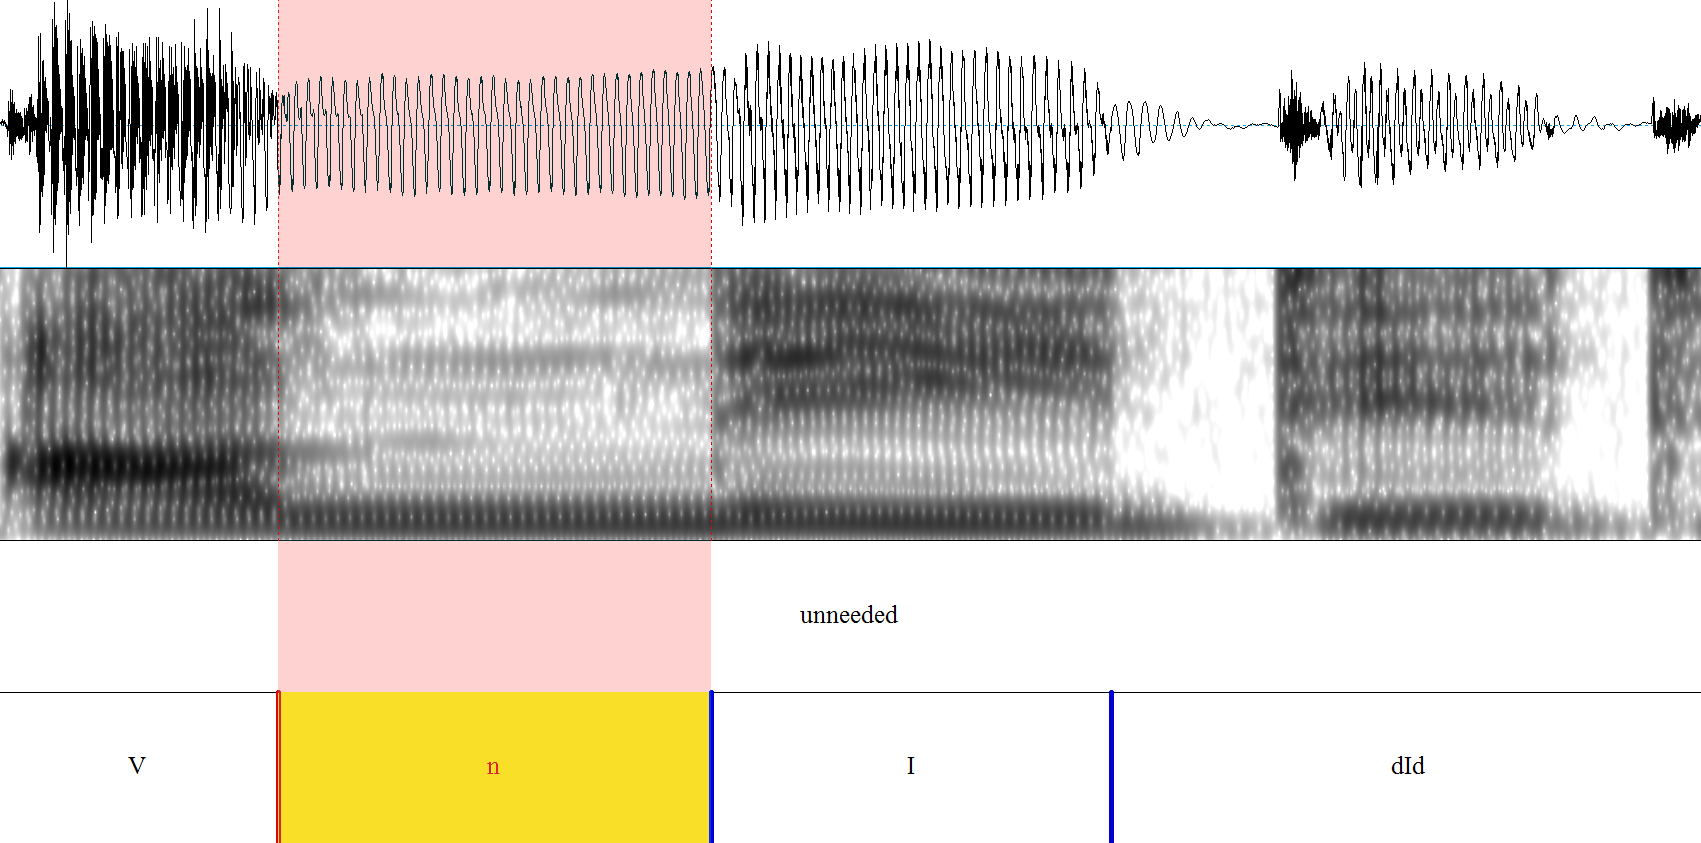
\includegraphics[width=11.5cm ,keepaspectratio]{images/GeneralMethod/segmentationUnneeded.png}}
	\caption{Segmentation example \textit{unneeded}}
	\label{fig:segmentation unneeded}
\end{figure*}

There are two possible ways of segmenting speech data, \is{phonetic segmentation}manual segmentation and \isi{automatic segmentation}. Automatic segmentation has the major advantage of demanding a lower workload and less time than \is{phonetic segmentation}manual segmentation. Furthermore, one can expect \isi{automatic segmentation} to be very systematic. This is because \isi{automatic segmentation} relies on forced aligners which are based on algorithms. These algorithms ensure that every file is segmented according to the same criteria. This means, in contrast to \is{phonetic segmentation}manual segmentation, there is no risk of inter-annotator differences.

However, there are also major disadvantages with \isi{automatic segmentation}. The forced aligners used in \isi{automatic segmentation} rely on canonical pronunciations. This means that the forced aligner will always annotate all phonemes represented in the canonical pronunciation of a word, irrespective of whether they were produced by the speaker or not.  Especially in \isi{conversational speech} words are sometimes drastically reduced, i.e not all sounds of a word are produced. This poses a serious problem for \isi{automatic segmentation}. Segments which are not present are annotated by the system.
An additional problem is related to the fact that forced aligners do not analyze the whole sound file but instead analyze the file in increments of a few milliseconds. The forced aligner software WebMAUS (\citealt{Schiel.1999,Kisler.2016}), for instance, uses 10 ms increments. Especially when investigating fine \isi{phonetic detail} these increments are problematic. For example, the duration of a word-medial /l/ is 40 ms on average (cf. \citealt{Umeda.1977}). Increments of 10 ms might distort the phonetic investigation of the duration of /l/ immensely by positioning a boundary 10 ms too early, or 10 ms too late, i.e. the \isi{automatic segmentation} might show /l/ to be up to 50\% shorter or longer than it actually is.

To test the accuracy of \isi{automatic segmentation}, i.e. to test whether \isi{automatic segmentation} can be used in this study, I carried out an \isi{automatic segmentation} on a subset of the corpus and the experimental data. I used the software WebMAUS (\citealt{Schiel.1999,Kisler.2016}) for the segmentation.  WebMAUS takes speech files with orthographic transcriptions as an input and gives segmented, phonologically transcribed text grids as an output. The segmentation is based on a production system, which takes the canonical pronunciations of an utterance, as well as its sound wave, and then, on the basis of a Viterbi alignment procedure, computes the most probable pronunciation variant. Based on this pronunciation variant the speech wave is segmented in 10 ms increments. 
 
 
 The \isi{automatic segmentation} of the subset showed that the \isi{automatic segmentation} is inaccurate and therefore not suited to investigate fine \isi{phonetic detail}. As expected, the system annotated sounds which were not present in the acoustic signal and misplaced boundaries, i.e. boundaries were set too early or too late in the speech signal. Especially for the corpus data the boundaries were very poorly placed. This might be due to the extreme \isi{reduction} found in \isi{conversational speech}. 
 Having a valid, reliable and precise segmentation is extremely important for this investigation. Therefore, it was decided to not use \isi{automatic segmentation} but instead segment all sound files manually. I decided to not first use \isi{automatic segmentation} and then adapt the set boundaries since revising the \isi{automatic segmentation} holds the risk of influencing the annotator unconsciously. 
 

In contrast to \isi{automatic segmentation}, \is{phonetic segmentation}manual segmentation is less prone to systematic mistakes and inaccuracies. This is because it does not rely on canonical representations and incremental analyses. It thus allows for more precise annotations than \isi{automatic segmentation}.  However, there are also disadvantages with \is{phonetic segmentation}manual segmentation. 
First, it is very time-consuming. Second, it is prone to inconsistent, unsystematic boundary setting, as well as to inter-annotator differences. While the possibilities to speed up \is{phonetic segmentation}manual segmentation are very limited, there are various possibilities to prevent inconsistencies and inter-annotator differences. To ensure the reliability and validity of the \is{phonetic segmentation}manual segmentation, I applied the following four strategies: 1.  the development of strict segmentation criteria based on the specifics of each sound, 2.  intensive training of the annotators, 3. segmenting a proportion of the data twice, and 4. testing the influence of the annotator on the segmentation statistically. In the following, I will discuss each strategy in detail.\\


\textbf{1. The development of strict segmentation criteria}\\

The criteria on which the segmentation was based were developed by consulting  the relevant phonetic literature (cf. \citealt{Ladefoged.1996,Johnson.1997b,Ladefoged.2003,Machac.2009,Ladefoged.2011}) and were optimized during the segmentation process. The final criteria will be described in the following. First, I will describe the criteria for the segmentation of the nasals in \is{un-}\prefix{un} and \is{in-} \prefix{in}words. Then, I will give a description of the criteria for fricatives in \is{dis-}\prefix{dis}words. Finally, the criteria for laterals in \is{-ly}\suffix{ly}-words will be given.\\



\textbf{The nasals in \prefix{un} and \prefix{in}prefixed words}\\

Nasals have a regular waveform which has a lower amplitude than the waveform of vowels. Formants of nasals are quite low and faint in comparison to those of vowels. Boundaries between the preceding vowel and the nasal were thus set where the acoustic energy drops in the waveform, the spectrogram becomes visbily fainter and the higher formants visibly decrease (see \figref{fig:segmentation unneeded}). In case of a following vowel, the boundary was marked at the point where the amplitude increases in the waveform and the formants become clearly visible (see \figref{fig:segmentation unneeded}).  Since approximants have, similar to vowels,  a higher amplitude than nasals, as well as more acoustic energy, the identification of approximants following the nasal was similar to the identification of a following vowel. If a stop followed the nasal, the boundary was marked at the beginning of the occlusion, which was identified by the abrupt decrease of the waveform and the sudden diminishment of the formants (see \figref{fig:segmentation imprint}). In case of a following fricative, the boundary was set where the waveform became visibly irregular and the energy was concentrated in the upper part of the spectrogram with no distinct formants visible. All boundaries were set at the nearest zero crossing of the waveform.\\



\begin{figure} 
	\fbox{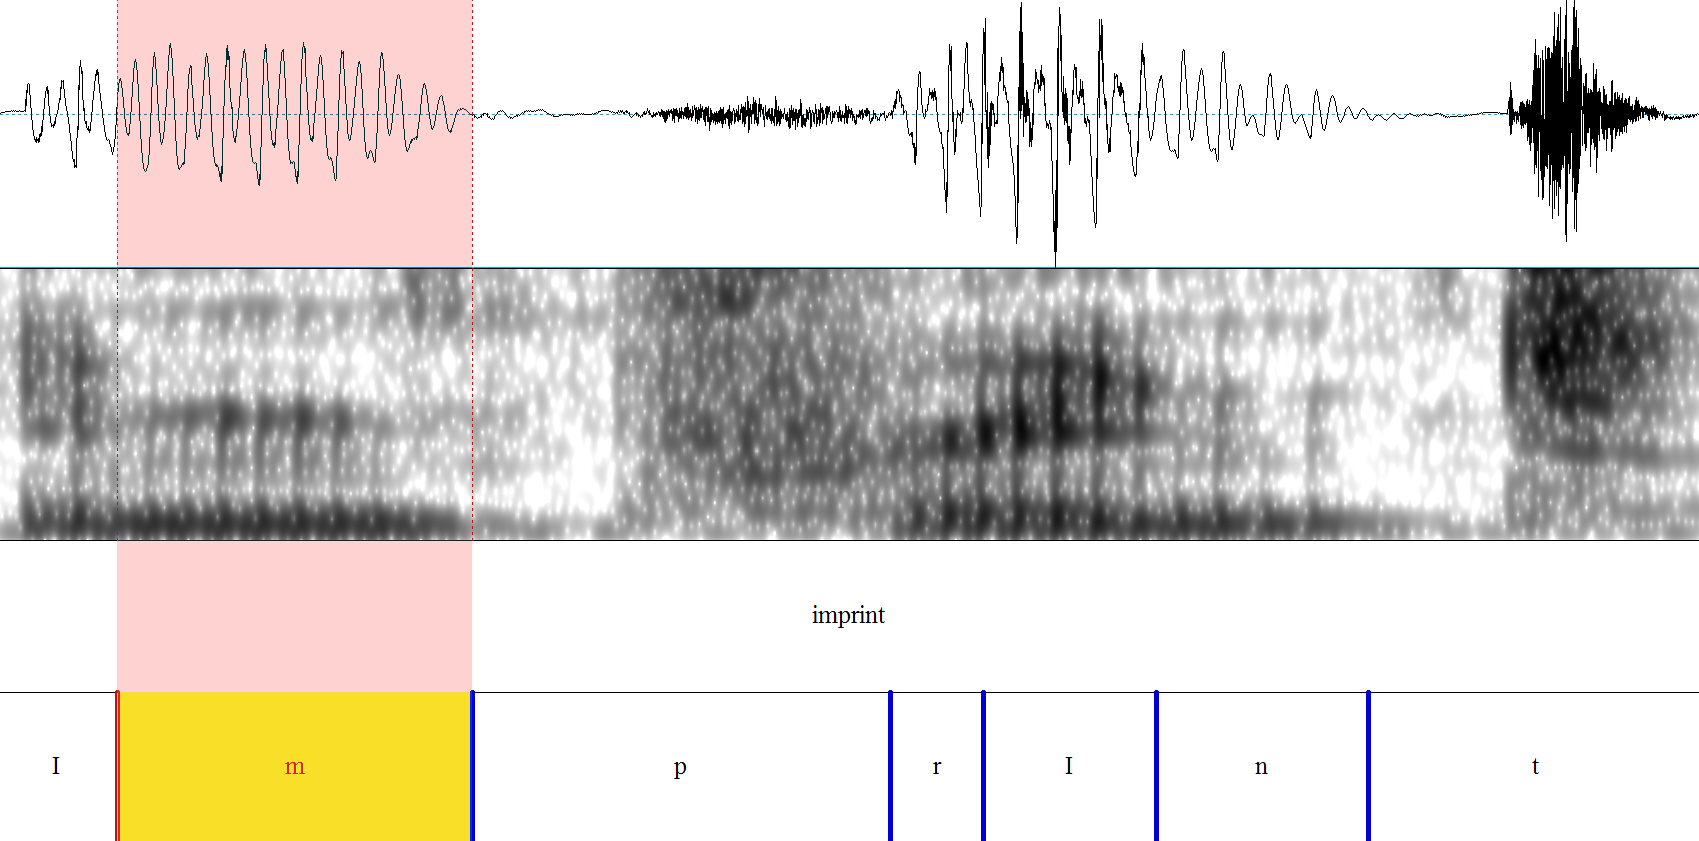
\includegraphics[width=11.5 cm ,keepaspectratio]{images/GeneralMethod/segmentationImprint.png}}
	\caption{Segmentation example \textit{imprint}}
	\label{fig:segmentation imprint} 
\end{figure}


\textbf{The fricative in \prefix{dis}prefixed words}\\




Fricatives are characterized by an irregular waveform, which is very easy to distinguish from the regular waveform of vowels. Furthermore, for fricatives, there is energy throughout the whole spectrogram and no separate formant bands are visible. Most energy is visible in the upper part of the spectrogram (see \figref{fig:segmentation dissident}). This is even more pronounced for voiceless fricatives, which are found in the majority of the \is{dis-}\prefix{dis}prefixed words.
The boundary between the preceding vowel and the fricative was set where the waveform became irregular and the distinct formant structure vanished. The boundary between /s/ and the following vowel was set where the opposite was the case (see \figref{fig:segmentation dissident}). In case of a following approximant, the same criteria were applied. If a stop followed the fricative, the boundary was marked at the beginning of the occlusion. There were no fricatives immediately following the prefixal /s/ in the data sets.\\

\begin{figure} [H]
	
	\fbox{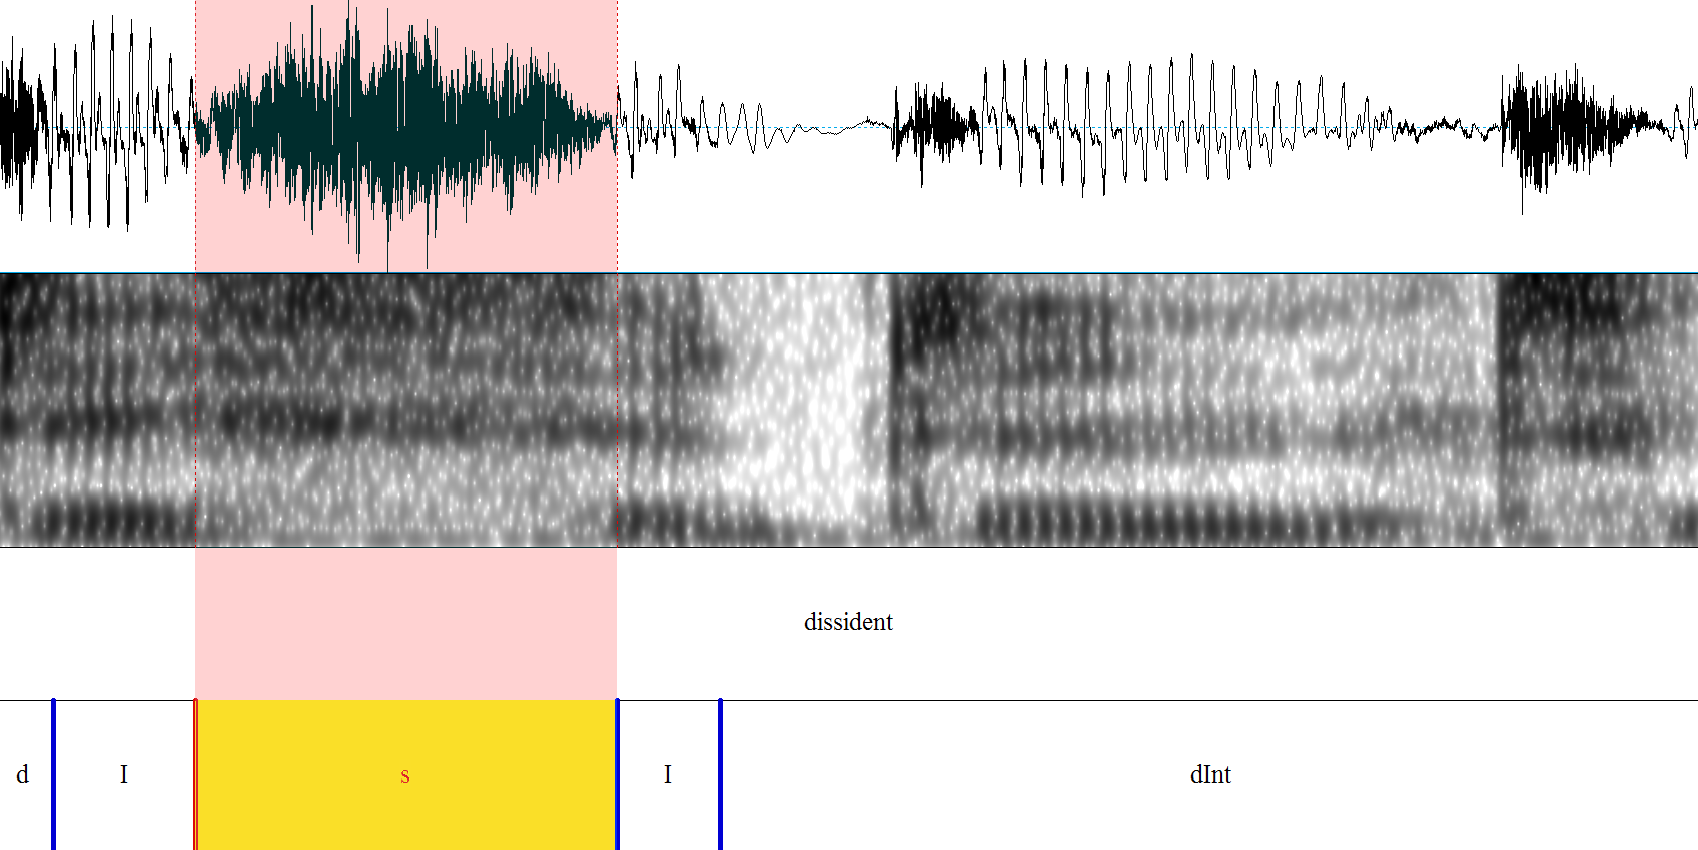
\includegraphics[width=11.5 cm ,keepaspectratio]{images/GeneralMethod/segmentationDissident.png}}
	\caption{Segmentation example \textit{dissident}}
	\label{fig:segmentation dissident}
\end{figure}



\textbf {The lateral in \suffix{ly}-suffixed words} \label{ly-segmentation}\\



% Most difficult segment to segment in data set --> a ot of exlcusion

Out of the four consonants investigated in this study, laterals are the most difficult to segment. This is due to the fact that laterals are very similar to vowels regarding their acoustical properties. Thus, it is quite challenging to set a boundary between vowels and laterals (see also \citealt[chapter 7]{Machac.2009} for discussion). However, there are some aspects in which /l/ can be distinguished from vowels. There is less amplitude in the waveforms of laterals than in the one of vowels.  Furthermore, their formant structure is, in contrast to the one of vowels, constant and, due to less energy in the speech signal, the formants of /l/ are in general fainter than the ones of vowels. This is especially the case for higher formants. Since in the suffix -\textit{ly} the lateral is followed by a high vowel, which displays a high level of energy in the upper formants, it is possible to see the formant structure change between /l/ and the following vowel in my data sets. The boundary between /l/ and /i/ was thus set at the point at which the formant structure changed, i.e. the higher formants became more pronounced (see \figref{fig:segmentation solely}). For intervocalic /l/ a visible decrease in the waveform, as well as the change in formant structure was used to mark the beginning of /l/ (see \figref{fig:segmentation solely}).
 
\begin{figure*}  
	
	\fbox{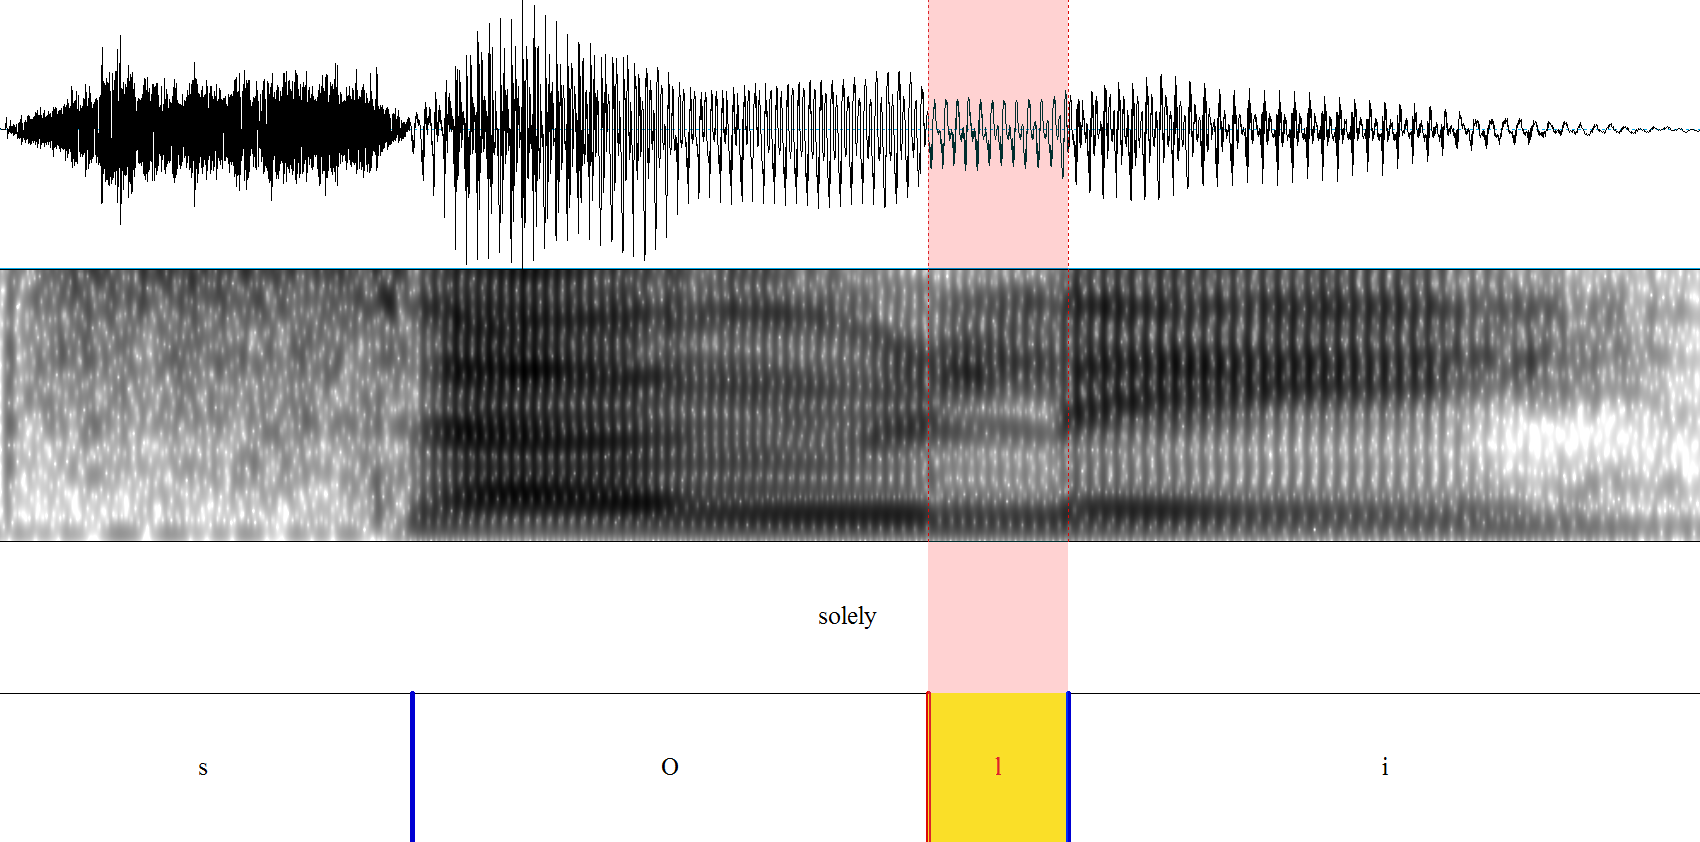
\includegraphics[width=11.5 cm ,keepaspectratio]{images/GeneralMethod/segmentationSolely.png}}
	\caption{Segmentation example \textit{solely}}
	\label{fig:segmentation solely}
\end{figure*}


Setting the boundaries between /l/ and a preceding consonant was generally not problematic since approximants can be distinguished quite easily from nasals, stops and fricatives. Approximants generally have a  higher amplitude and more energy in the spectrogram than nasals. Their waveform is periodic, whereas the waveform of fricatives, as well as the waveform of the aspirational phase of stops, is irregular.



\begin{figure*}  
	
	\fbox{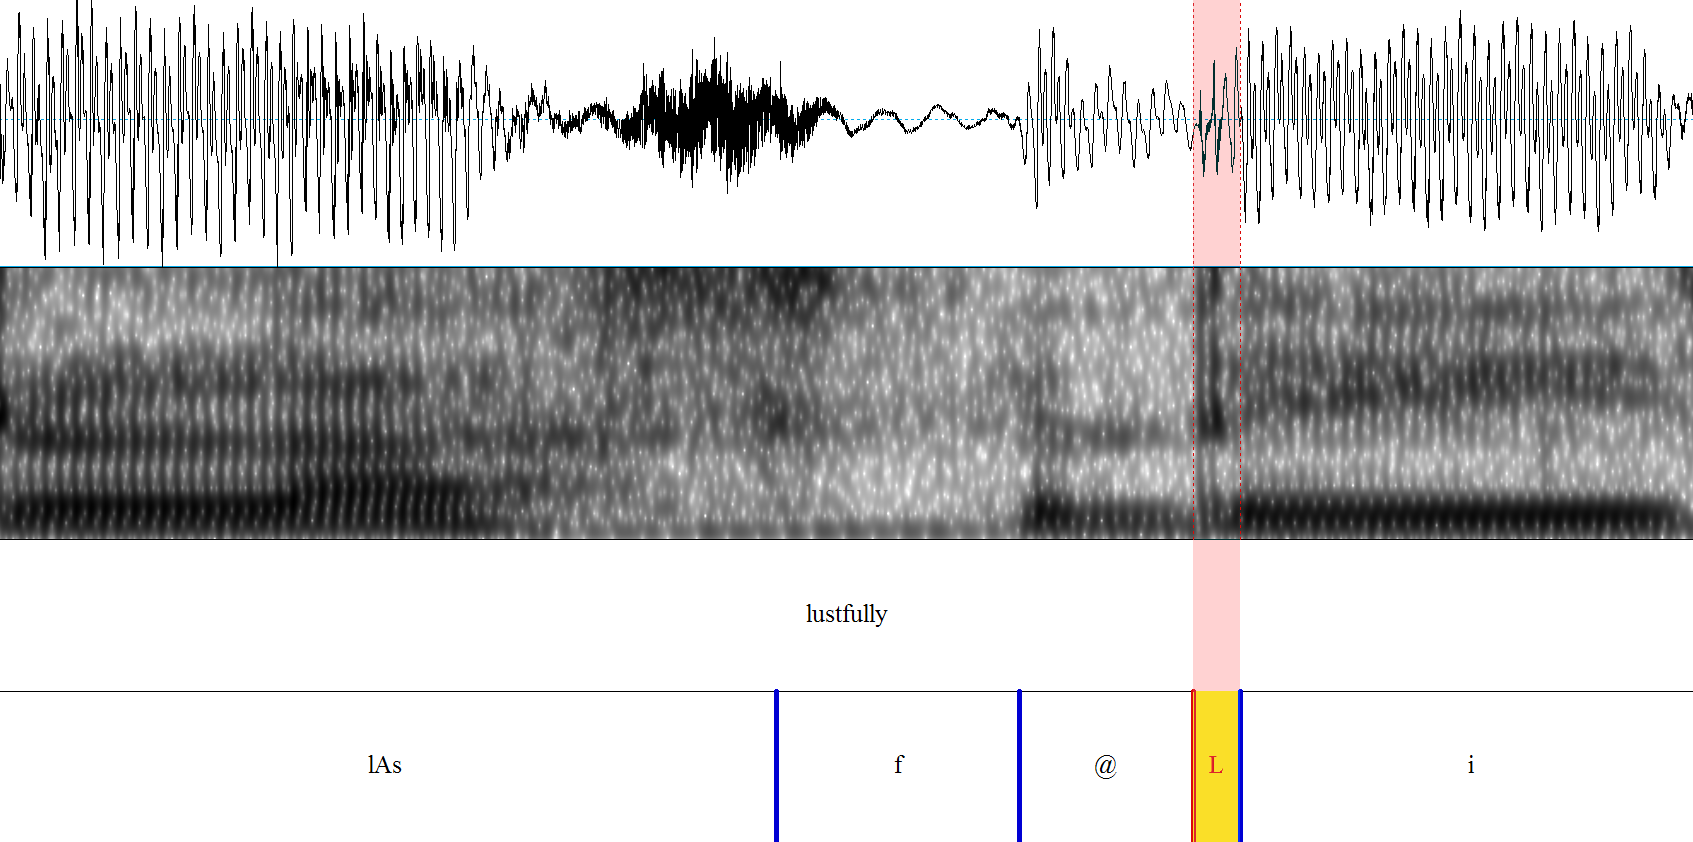
\includegraphics[width=11.5 cm ,keepaspectratio]{images/GeneralMethod/segmentationLustfully.png}}
	\caption{Segmentation example \textit{lustfully}}
	\label{fig:segmentation lustfully}
\end{figure*}


%\enlargethispage{1\baselineskip}
In some cases the waveform and the spectrogram for /l/ showed a completely different pattern. \figref{fig:segmentation lustfully} shows a case in which /l/ is marked by a dark, vertical bar which stretches throughout the whole spectrogram. In this case /l/ is realized as a tap, i.e. not as an approximant. The bar marks the tongue release from the alveolar ridge. Because of the high amount of energy in the spectrogram /l/ can be easily set apart  from the neighboring vowels. This type of /l/ , i.e. a tap /l/, is generally shorter than the one described above, i.e. the approximant /l/. To account for this difference in duration the type of /l/ pronounced was coded in the variable \textsc{TypeOfL}. The variable was then incorporated in the statistical models as a covariate.\\

% very problematic at end of word - base words, often allomorphy, sometimes not visible at all



\begin{figure*} [b!]
	
	\fbox{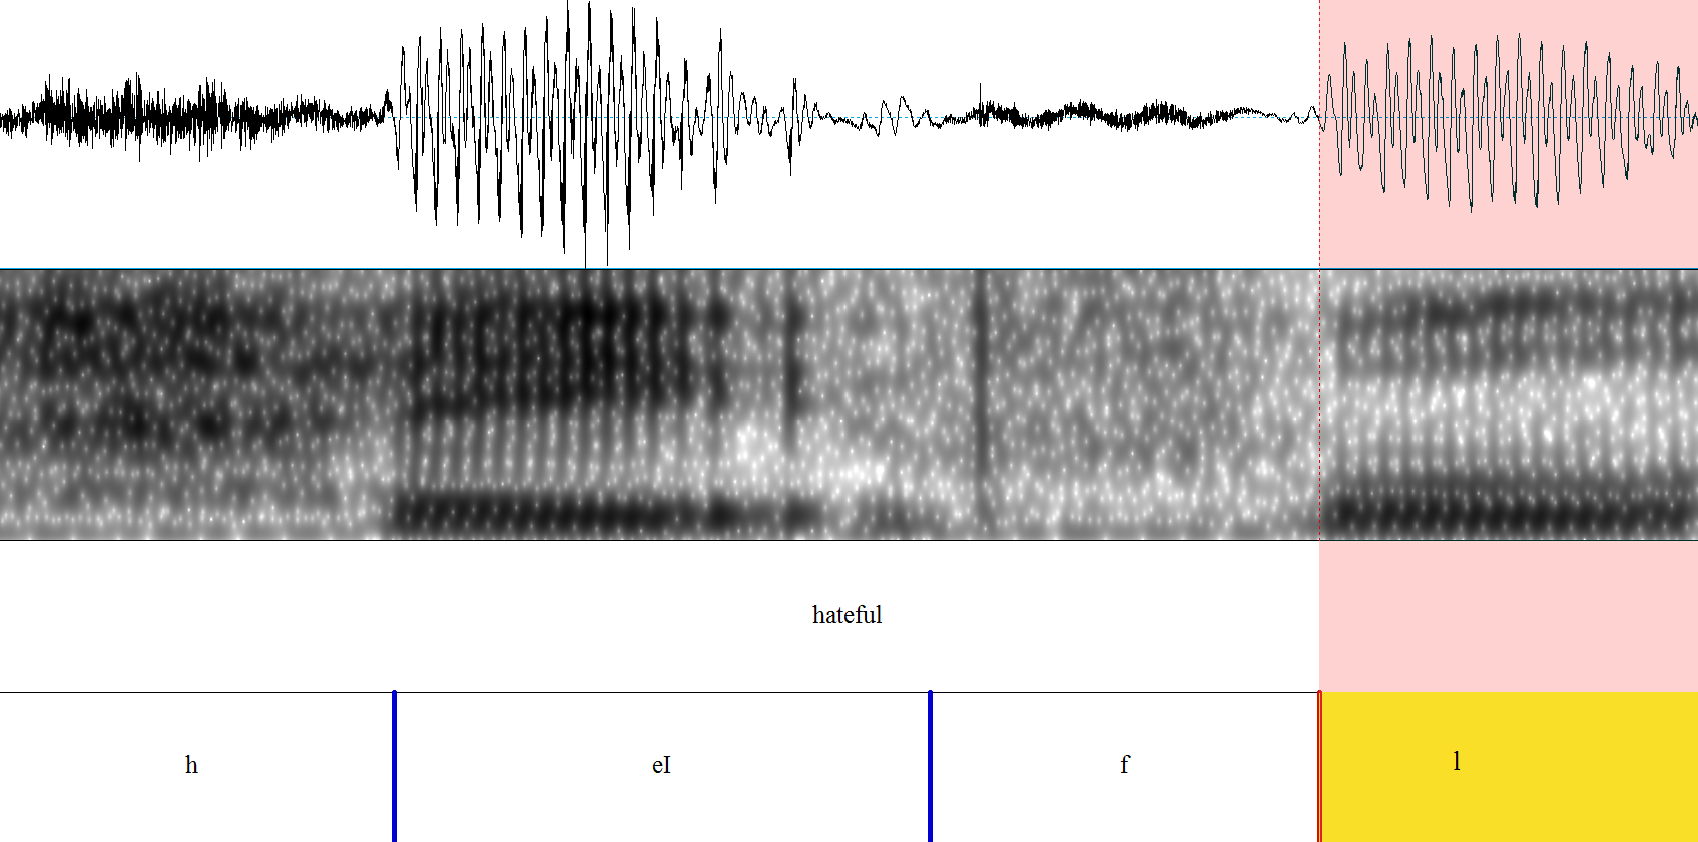
\includegraphics[width=11.5 cm ,keepaspectratio]{images/GeneralMethod/segmentationHateful2.png}}
	\caption{Segmentation example \textit{hateful}}
	\label{fig:segmentation hateful}
\end{figure*}

The criteria described above allowed for a valid and reliable segmentation of /l/. However, there were still items which were very difficult to segment. This was especially the case for items of the category l\#, i.e. /l/ at the end of base words (e.g. \textit{hateful, cool}). An example is displayed in \figref{fig:segmentation hateful}. There is no visible boundary between the preceding vowel and the lateral, i.e. the speaker did not pronounce them as two distinct sounds. There are various possible explanations, such as that the speaker might have deleted the word-final /l/, or that he might have vocalized it  while deleting the preceding vowel. Either way,  it is impossible to set a valid boundary between /l/ and the preceding vowel. Therefore, we marked the whole interval as /l/ (see \figref{fig:segmentation hateful}) and coded the pertinent tokens as featuring a vocalized /l/. Hence, the data set comprised three different types of /l/: the approximant /l/, the tap /l/ and the vocalized /l/. These three different types were coded in the variable \textsc{TypeOfL} with the values \texttt{approximant}, \texttt{tap} and \texttt{vocalized}.\\



\textbf{ 2.  Intensive training of the annotators}\\
% training

The corpus data was segmented by five annotators. The experimental data was segmented by six. The reliability of the segmentation criteria was verified by a set of trial segmentations.  In these trials the annotators segmented the same 30 items. If boundaries differed by more than 10 milliseconds, the annotators discussed the discrepancy and refined the criteria in order to reduce inter-annotator variation. The trial segmentations were repeated two times until all boundaries were reliably placed with only small variations, i.e. variations within 10 ms. For the final measurement, each annotator worked on a disjunct set of items. If an annotator was not confident concerning the segmentation of an item, the item was discussed with all annotators. Items which could not be validly segmented were excluded. This was the case for several of the corpus items due to the poor quality of the sound files, as well as for various items including /l/. \\%All in all ...items were excluded from the corpus data, and ...items were excluded from the experimental data.

\textbf{ 3. Segmenting a proportion of the data twice}\\

To further ensure reliability, 10~\% of each annotator's items were segmented by a second annotator. These 10~\% were then compared. Discrepancies between the segmentations were discussed and systematic mistakes were detected. To correct these mistakes, and to avoid them in future codings, the segmentation criteria were clarified and enhanced. The annotators revised all previous segmentations according to the enhanced criteria.\\

%\newpage
% stats

\textbf{ 4. Testing the influence of the annotator on the segmentation statistically}\\

After the segmentation process was completed, a script was used to measure and extract word duration, the duration of the consonants in question and the duration of the preceding and the following segments in milliseconds. For each subset,  I compared the segmentations of each annotator by checking whether the durations varied significantly across annotators.
 For the comparison, I used linear models in which the dependent variable was the duration of the consonant in question (e.g. /n/ for \prefix{un}prefixed words). I tested whether consonant duration varied significantly by annotator. The models revealed that the annotator did not have any effect on the duration of the consonant, i.e. the segmentation did not vary significantly across annotators.


\section{Statistical analyses}\label{stats}

In both studies similar statistical analyses were used to investigate {morphological gemination}. All statistical modeling was carried out using the software R (\citealt{RDevelopmentCoreTeam.2014}). 
The main analyses in all studies consisted of the investigation of the duration of the consonant in question. 
In this section, I will give an introduction to the statistical models fitted to investigate duration. In addition to general information about the statistical procedures applied, I will discuss pertinent problems and explain how they were approached. The details of each model, as well as problems with specific data sets, will be described in the pertinent sections. Statistical procedures which were only relevant for specific subsets of the data will also be discussed in the pertinent sections. 




% distribution categorical vs. gradient
This first durational analysis in both studies consisted of investigating the distributions of consonant duration across different environments. This investigation is of importance with regard to the question of whether \isi{gemination} is a categorical or a gradient phenomenon (see \sectref{Morphological Gemination} and \sectref{decomposability} for discussion). If \isi{gemination} is a categorical phenomenon, the data should show a bimodal distribution. If \isi{gemination} is a gradient phenomenon, one would expect a gradient increase in duration from singletons to doubles.

 To investigate the distribution of duration across environments, boxplots were generated, and differences in average duration between environments were tested for significance by using standard statistical tests. Boxplots have the advantage of displaying a lot of information about the data's distribution simultaneously (e.g. median, the distribution of quartiles). Therefore, these graphs are very well suited to compare the distribution of two or more categories with each other (see, for example, \citealt{Benjamini.1988}).  
 I used boxplots to compare the durations of singletons with the durations of doubles. The plots show whether the distributions of singletons and doubles deviate, and whether the distribution of the whole data set (including singletons and doubles) is bimodal. If the distribution is bimodal, \isi{gemination} can be assumed to be categorical.
  In case of a non-bimodal distribution more advanced statistics are needed to test whether the data at hand shows (gradient) \isi{gemination}, or whether all morphological \is{morphological gemination}{geminates} in the data set {degeminate}.
 After the analysis of the raw data, more advanced statistical analyses were used to investigate \isi{gemination} and the factors influencing duration more thoroughly.


In both studies \isi{multiple regression} was used to test the effect of various factors on consonant duration. For each affix, i.e. each subset, at least one model was fitted (see \tabref{tbl: Overview categories in each study} for an overview of the subsets). The dependent variable in all models was consonant duration, i.e. the models predicted the duration of the affixational consonant. Consonant duration was measured in absolute and in relative terms. Relative duration refers to the duration of the consonant relative to the duration of its preceding segment. Models with both absolute and \isi{relative duration} were fitted for each affix.
The independent variables were mainly determined by the predictions made in the previous chapter and varied slightly across models. They will be presented in further detail in the next section.


Multiple regression was used since it is an established and highly successful way to deal with the multitude of factors involved in predicting durational properties of morphemes (see, for example, \citealt{Hay.2007}; \citealt{Hanique.2012}; \citealt{Smith.2012}; \citealt{Plag.2017}). Using this type of model one can investigate one specific predictor while simultaneously accounting for other, potentially intervening, predictors. One can thus, for example, test whether the number of consonants influences the duration of a consonant, while simultaneously taking other factors, such as \isi{speech rate} or \isi{stress} pattern, into account.  Another major advantage of \is{multiple regression}multiple regression models is their capability to deal with unbalanced data sets. Especially for the corpus data this is of high importance. 

% 2 problems - what is \isi{collinearity}
However, \is{multiple regression}multiple regression models also entail some statistical problems that need to be addressed. Two of them are especially relevant for the present analyses: \isi{collinearity} and \isi{overfitting}. Let us first discuss \isi{collinearity}.
A number of measurements I would like to include in the models are correlated, for example the number of segments in the word and word duration. A word which has more segments is most likely also longer in terms of duration. This can lead to serious problems in \is{regression model}{regression models} (\is{collinearity}{\textit{multicollinearity}}, for example, \citealt[chapter 6]{Baayen.2008}).  If one of the two variables has an influence on consonant duration, so will the other. This makes it difficult for the model to tease apart the individual explanatory power of each of the two variables. 

% How to deal with \isi{collinearity}
There are several possible strategies to deal with \isi{collinearity}. One strategy is to include only one of the correlating variables.  This is a conservative and safe strategy, which may, however, decrease the power of the model. If \isi{collinearity} only affects noise variables, i.e. variables which are known to affect the dependent variable but whose effect is not of primary interest for a study, another option is to keep the correlating variables in the model but not interpret their individual contribution to the model (cf. \citealt{Wurm.2014}). A third strategy is to combine factors. The two variables \textsc{NumberOfSegmentsInTheWord } and \textsc{WordDuration}, for example, can be combined by calculating the variable \textsc{SpeechRate}, which is computed by dividing word duration by the number of segments. Another possibility of combining factors is by conducting a principal components analysis. In this type of analysis the dimensionality of the data is reduced by transforming the different variables into so-called principal components. The transformation results in linear combinations of the predictors, i.e. the principal components, that are uncorrelated with each other (see, for example, \citealt[chapter 5.1]{Baayen.2008}; \citealt[chapter 12]{Venables.2011}). To address potential \isi{collinearity} problems, I applied all of the strategies mentioned above. 


 % \isi{overfitting}
 The second potential problem with \is{regression model}{regression models} is \isi{overfitting} (see, for example, \citealt{Draper.1998,Babyak.2004}). The number of variables included in a model must be appropriate for the number of observations in the data set. If this is not the case, the model cannot be trusted. In other words, if too many terms are included in a model, the model will not be able to adequately approximate the effects of the included variables. Note that the notion \textit{terms} not only refers to the number of predictor variables per se, but also to the number of variable levels and interactions included in the model.  A common rule of thumb states that 10--15 observations per term are necessary to avoid \isi{overfitting} (cf., for example, \citealt{Draper.1998}). Especially in the corpus data sets, which are of relatively small size, the number of variables included in the models had to be restricted, and the variables needed to be chosen carefully. 
 
% strategy for modelling \\
%\enlargethispage{\baselineskip}
Let us now turn to the modeling strategy which was adopted in all models. Following established practices in the field (e.g. \citealt{Baayen.2008}), I first conducted an initial model incorporating all variables whose effect was to be tested. I then checked the residuals of the model, which need to be normally distributed. If visual inspection revealed that the residuals had a non-normal distribution, transformations  and the exclusion of outliers were used to obtain the desired pattern. If a transformation of the dependent variable was necessary to alleviate problems of non-linearity, Box-Cox transformations were used to identify a suitable transformation parameter for a power transformation (see, for example, \citealt{Box.1964, Venables.2011}).

After the residuals showed a satisfactory distribution, I checked for \isi{collinearity} in the models by looking at the correlations between potentially correlated variables. In those cases where \isi{collinearity} was a potential problem, I followed the strategies described above.  In all models, I tested for relevant interactions. The strategy for testing interactions will be discussed in sections \ref{analyses dur corpus} and \ref{analsyses duration experiment}, after all variables included in the models are introduced.

The \is{regression model}{regression models} were then simplified by stepwise excluding insignificant predictors. A predictor was considered significant if its p-value was lower than 0.05, and if the Akaike Information Criterion (AIC) of the model including the predictor was lower than when the predictor was not included. A lower AIC indicates that a model including the factor has a greater explanatory power than a model without the predictor variable. Linear models were generated using the \texttt{lme4 package} (\citealt{Bates.2014}).

In addition to the stepwise exclusion of insignificant factors, i.e. finding the one model which explains the variation found in the data best, I also used \isi{multi-model inferencing} (see, for example, \citealt{Barth.2014}). Multi-model inferencing estimates the predictive value of each variable by looking at a multitude of possible models. Instead of just giving the significance of one variable in one specific model, it indicates the importance of a variable across a multitude of models. 
The importance of a variable is determined by the number of models in which the variable is significant and by the goodness of each model in which the variable is significant (measured in the AIC of the model). A variable which is significant in various models with a high AIC will have a high importance value. A variable which is significant in fewer models with a lower AIC will have a lower importance value. The \isi{multi-model inferencing} was carried out using the \texttt{MuMin package} (\citealt{Barton.2016}), and was used as an additional clue to assess which variables influence affixational consonant duration.

In addition to the durational analyses, statistical analyses were applied to investigate \isi{decomposability}. 
I investigated the relation of five different \is{decomposability measure}decomposability measures to find out whether these measures can be used as operationalizations of the same underlying concept. The investigated \is{decomposability measure}decomposability measures will be introduced in the next section. 
Furthermore, I compared the included affixes by means of the different \is{decomposability measure}decomposability measures to investigate their \isi{segmentability}. This analysis was conducted to find out whether the \isi{segmentability} hierarchies introduced in \chapref{affixes} are borne out by the data. 
The conducted \isi{decomposability} analyses will be explained in detail in the pertinent sections of Chapters~\ref{Corpus Studies} and~\ref{Experimental Studies}. 



\section{Coding of the variables} \label{General method annotation}


% annotated factors which influence consonant duration --> same in corpus and experimental study (comparison)

In both studies the data was annotated with regard to factors which potentially influence consonant duration and \isi{gemination}. The annotation of the data resulted in the coding of various variables.
 These variables can be divided into two groups: variables of interest and noise variables. Variables of interest are those variables which are used to test the predictions made in \chapref{Theory}. In other words, these variables serve to test the effects of the factors predicted to govern \isi{gemination} according to the different theoretical approaches (see \tabref{tbl:Factors predicting gemination} for an overview of these factors).
Noise variables, on the other hand, are those variables which are known to influence consonant duration but which are not directly linked to the predictions made by the theoretical approaches discussed.

There are seven variables of interest. The first one is \textsc{Environment}. This variable was coded to answer the question of whether an affix {geminates}. It holds information about the morphological and phonological environment of the investigated consonant(s) and is essential for all predictions.


%, including the number of consonants and the consonant-adjacent segment. 
Five variables of interest are closely related to the notion of \isi{boundary strength},  and form possible operationalizations of \isi{decomposability}. The five variables are \textsc{SemanticTransparency}, \textsc{SemanticTransparencyRating}, \textsc{TypeOfBase}, \textsc{RelativeFrequency} and \textsc{LSAScore}. As will be laid out below in further detail, they are relevant for the majority of the predictions made in \chapref{Theory}. 


The last variable of interest is \textsc{Affix}, which codes for the affix itself. On the one hand, this variable is needed to answer the question of which affix {geminates}. On the other, it is necessary for the comparison of affixes with regard to their \isi{segmentability}. This comparison is of importance for the affix-specific predictions made by the \isi{decomposability} and the \is{informativeness}morphological informativeness approach (see \sectref{summary predictions} for discussion). 


For the most part, the same variables were included in all analyses. However, due to differences between corpus and experimental data, some variables were only used in one of the two studies. 
 Furthermore, affix-specific features, such as the phonological make-up of an affix, called for the inclusion of additional variables in some of the models (e.g. \textsc{Voicing} for \is{dis-}\prefix{dis}). Inherent differences between affixes also led to some minor differences in the coding of some variables across subsets, e.g. in the variable \textsc{Environment}. 
 
Below I will describe all variables which were initially considered in all models, including the ones only considered for the models of specific subsets. I will describe why the variable is of interest for the study and how it was coded. Differences in the coding between subsets will also be discussed. Furthermore, I will lay out  problems with regard to the testing of some of the variables, and I will briefly discuss how these problems were dealt with. The specific modeling procedure with regard to the inclusion of certain variables will be discussed in the pertinent sections of this book.


First, I will describe the variables of interest. Then, I will turn to the noise variables, which can be categorized  into three different types: phonetic factors, phonological factors and lexical factors.  Finally, I will give an overview of which variables were included in which study. 

\subsection{Variables of interest} \label{variables of interest}

\textbf{Environment.}  The variable \textsc{Environment} was coded to test whether a word \is{gemination}{geminates}. It codes the phonological and the morphological environment of the consonant(s) investigated in a particular word. The variable is based on the four different structures included in the two studies,  i.e. phonological doubles in complex words, orthographic doubles in simplex words, singletons in complex words and singletons in bases. This means that every level coded in the variable represents one of the four structures. In \sectref{General Method Data Sets}, the different structures and their environments were already introduced. %The environments differ from each other in four respects.
 
 \tabref{tbl:Levels of the variable Environment} gives an overview of the levels of the variable \textsc{Environment} for the prefixes \is{un-}\prefix{un}, \is{in-} \prefix{in} (for both allomorphs\is{allomorphy}) and \is{dis-}\prefix{dis}. For each level examples are given.
 For \is{un-}\prefix{un} and /ɪn/ four environments exist. For the allomorph /ɪm/ three environments exist, and for \is{dis-}\prefix{dis} five environments were coded.\footnote{In \sectref{General Method Data Sets} the composition of the data sets is explained in detail, i.e. it is explained why for some affixes fewer environments were included in the investigation than for others.}
 

 
 \begin{table*}
 	\caption{Levels of the variable \textsc{Environment} for \prefix{un}, \prefix{in} and \prefix{dis}}
 	\label{tbl:Levels of the variable Environment}
 	
 		\begin{tabular} {llll}
 			\lsptoprule	
 			\textbf{un-}&&&\\
 			\textsc{Environment} & Example & &\\
 			\midrule
 			\texttt{n\#nV}&\color{lsMidBlue}\textit{unnatural} &&\\ 
 			\phantom{n }\texttt{\#nV}&\color{lsMidBlue}\textit{natural}& &\\
 			\texttt{n\#C}&\color{lsMidBlue}\textit{untold} && \\ 
 			\texttt{n\#V}&\color{lsMidBlue}\textit{uneven} &&\\
 			%\midrule
 			\midrule
 			\\
 			
 			
 			\textbf{in-}&&\textbf{im-}&\\
 			\textsc{Environment }& Example &\textsc{ Environment} & Example\\
 			\midrule
 			\texttt{n\#nV}&\color{lsMidBlue}\textit{innumerous} &\texttt{m\#mV}&\color{lsMidBlue}\textit{immortal}\\ 
 			\phantom{n}\texttt{\#nV}&\color{lsMidBlue}\textit{numerous} &\phantom{n}\texttt{\#mV}&\color{lsMidBlue}\textit{mortal} \\ 
 			\texttt{n\#C}&\color{lsMidBlue}\textit{intolerant} &\texttt{m\#C}&\color{lsMidBlue}\textit{impossible} \\ 
 			\texttt{n\#V}&\color{lsMidBlue}\textit{inefficient}  &  \\ 
 			\midrule     	
 			%\midrule
 			
 			\\
 			
 			\textbf{dis-}&&&\\
 			
 			
 			\textsc{Environment}& Example && \\
 			\midrule
 			\texttt{s\#sV}&\color{lsMidBlue}\textit{dissatisfied} && \\ 
 			\phantom{s}\texttt{\#sV}&\color{lsMidBlue}\textit{satisfied} && \\ 
 			\texttt{s\#C}&\color{lsMidBlue}\textit{disgrace} & &\\ 
 			\texttt{s\#V}&\color{lsMidBlue}\textit{disarm} && \\ 
 			\texttt{sV}&\color{lsMidBlue}\textit{dissertation} && \\ 
 			\lspbottomrule   	
 			%\midrule
 			
 			
 		\end{tabular}
 	
 	
 \end{table*}
 
  
  On the one hand the variable \textsc{Environment} codes the number of underlying segments found in each word, on the other the segment following the consonant of interest and the presence/absence of a morphological boundary is coded.  With regard to the number of consonants,  words featuring the environment \texttt{n\#nV}, \texttt{ m\#mV} and \texttt{s\#sV} feature two identical consonants. All other environments only feature one corresponding underlying segment. 
  To test \isi{gemination}, one can test whether underlying doubles, i.e. the consonants in \texttt{n\#nV}-,  \texttt{m\#mV}- and \texttt{s\#sV}-words, are longer than the corresponding singletons in the other investigated structures. For example, if the nasal in \textit{unnatural} (\texttt{n\#nV}) is longer than the nasal in \textit{natural} (\texttt{\#nV}), the nasal in \textit{untold} (\texttt{n\#C}) and the nasal in \textit{uneven} (\texttt{n\#V}), the word \textit{unnatural} {geminates}.
  
  The existence of different environments with an underlying singleton can be explained by referring to three of the four investigated structures, i.e. singletons in complex words, singletons in bases and orthographic doubles in simplex words. The different levels represent the three different structures, i.e. singletons in complex words are coded as \texttt{n\#C}, \texttt{n\#V}, \texttt{m\#C}, \texttt{s\#C} and \texttt{s\#V} , singletons in bases are coded as \texttt{\#nV}, \texttt{\#mV} and \texttt{\#sV}, and orthographic doubles are coded as \texttt{sV}. Note that the \textit{\#} marks a morphological boundary.
  While singletons in complex words were included to compare durations of doubles and singletons in comparable structures, singletons in base words were included to ensure that the potential lengthening of the double consonant is not due to an inherently long base-initial consonant. Orthographic doubles in simplex words were included to test the influence of \isi{orthography} on \isi{gemination} (see sections \ref{corpus data composition} and \ref{experiment data composition} for a thorough discussion of the investigated structures and their relevance for the investigation).
  
  

Let us now turn to the second important aspect coded in the variable, the segment following the consonant of interest. The following segment is only relevant for singletons in complex words. This is because in all other structures the  consonant of interest is always followed by a vowel, i.e. we do not find variability.  
As already noted in \sectref{General Method Data Sets}, it is very important to account for the difference between a following vowel and a following consonant. The reason is that the following segment might affect the duration of the consonant of interest. This is evidenced by phonetic studies which show that the duration of consonants heavily depends on the neighboring segment (see, for example, \citealt{Umeda.1977}).  For nasals,  following vowels lead to shorter durations, following consonants increase it. For voiceless fricatives, a following vowel leads to a longer duration than a following consonant. For voiced fricatives, the following segment does not influence duration (\citealt[854]{Umeda.1977}). To code for possible influences of the following segment, two different levels for singletons in complex words were coded for each affix, singletons in complex words followed by a vowel (\texttt{n\#V}, \texttt{s\#V}) and singletons in complex words followed by a consonant (\texttt{n\#C}, \texttt{m\#C}, \texttt{s\#C}). Note that for the allomorph /ɪm/, no singletons in complex words followed by a vowel could be included. This is because in /ɪm/-prefixed words singletons are always followed by a consonant.


The coded environments for the suffix \is{-ly}\suffix{ly} deviate from the ones coded for the prefixes. 
As can be seen in \tabref{tbl:Levels of the variable Environment ly}, all in all six different levels were coded for \is{-ly}\suffix{ly}. Out of these six levels two feature an underlying double consonant (\texttt{l\#l}, \texttt{\is{syllabicity}syllabic l\#l}), and four an underlying singleton  (\texttt{l\#},  \texttt{\#l}, \texttt{\is{syllabicity}syllabic l\#} , \texttt{l}). The four different singleton levels correspond to the three singleton structures investigated, i.e. singletons in complex words (\texttt{\#l}), singletons in bases ( \texttt{l\#}, \texttt{syllabic} \texttt{l\#}) and orthographic doubles in simplex words (\texttt{l}).

 
 \begin{table*} 
 	\caption{Levels of the variable \textsc{Environment} for \suffix{ly}}
 	\label{tbl:Levels of the variable Environment ly}
 	
 		\begin{tabular} {llll}
			\lsptoprule
 			\textbf{-ly}&&&\\
 			
 			
 			\textsc{	Environment}& Example && \\
 			\midrule
 			\texttt{l\#l}&\color{lsMidBlue}\textit{really} && \\ 
 			\texttt{\is{syllabicity}syllabic l\#l}&\color{lsMidBlue}\textit{ment(a)lly} && \\ 
 			\texttt{l\#}&\color{lsMidBlue}\textit{real} && \\
 			 \texttt{\is{syllabicity}syllabic l\#}&\color{lsMidBlue}\textit{ment(a)l} && \\  
 			\texttt{\#l}&\color{lsMidBlue}\textit{probably}, \color{lsMidBlue}\textit{truly} & &\\ 
 			\texttt{l}&\color{lsMidBlue}\textit{belly} && \\ 
 			\lspbottomrule   	
 			
 			
 		\end{tabular}
 	
 \end{table*}
 

 
 The difference between the two environments with an underlying double, as well as the difference between the two environments for base words, is \isi{syllabicity}. In base words and words featuring a underlying double, the lateral sometimes is \is{syllabicity}syllabic. This occurs quite often when the base ends in the suffix \textit{-al} (e.g. in \textit{educationally/educational} or \textit{mentally/mental}). The schwa-preceding /l/ is deleted, and /l/ becomes \is{syllabicity}syllabic. The literature often claims that \is{syllabicity}syllabic consonants have longer durations than non-\is{syllabicity}syllabic consonants (see, for example,\citealt[67]{Jones.1959}; \citealt[135]{Clark.1995}; \citealt[329]{Price.1981}). This claim is, however, only partly supported by empirical research. For instance, while \cite{Toft.2013} has shown that \is{syllabicity}syllabic /l/ is longer than non-\is{syllabicity}syllabic /l/, a study by \cite{Barry.2000} has found the opposite. To consider possible effects of \isi{syllabicity}, I coded this factor in the variable \textsc{Environment}.  If in a pertinent word (e.g. \textit{mentally, mental}) the vowel preceding /l/ was deleted, i.e. the vowel was neither detected in the waveform, nor in the spectrogram, the word was coded as \is{syllabicity}syllabic. Hence, two levels for doubles in complex words and two levels for doubles in base words emerged (\texttt{l\#l}, \texttt{\is{syllabicity}syllabic l\#l},  \texttt{l\#}, \texttt{\is{syllabicity}syllabic \#l}.) 
 

As for the prefixed words, the consonant-adjacent segment might influence the duration of the consonant of interest in \is{-ly}\suffix{ly}-words. For laterals, a preceding consonant leads to shortening (\citealt[851]{Umeda.1977}). Therefore, one must code for the type of preceding segment in \is{-ly}\suffix{ly}-suffixed words. 
To prevent the variable \textsc{Environment} from featuring too many levels, I coded the type of preceding segment in a separate variable (\textsc{PrecedingSegment}) for \is{-ly}\suffix{ly}. The variable had two levels: \texttt{consonant} and \texttt{vowel}. \\


\textbf{Semantic Transparency.} The factor \isi{semantic transparency} is important for testing the predictions made by the \isi{prosodic word approach}, the morphological \isi{segmentability} approach and the \is{informativeness}morphological informativeness approach. 
The variable represents one way of operationalizing \isi{decomposability}. It has been used extensively in psycholinguistic research to investigate the question of whether words are processed as wholes or whether they are decomposed into their constitutent morphemes (see, for example, \citet{MarslenWilson.2009} for an overview). These studies have shown that transparent words are more easily decomposed than non-transparent words. Thus, there is some evience that \isi{semantic transparency} might be a well-suited measure of \isi{decomposability}. 

To test the pertinent predictions, and to investigate the suitability of \isi{semantic transparency} as a measure of \isi{decomposability}, I created the variable \textsc{Semantic-Transparency}. In the variable I coded whether the meaning of a derivative was transparent or opaque.
I checked the meaning of each derivative, as well as the meaning of its base, in the online version of the \textit{Oxford English Dictionary} (\citealt{OED.2013}).  If the meaning of the derivative is fully compositional, i.e. it can straightforwardly be computed by combining the meaning of the affix with the meaning of the base, it was categorized as \texttt{transparent}. 
Examples of transparent words are \textit{unnatural} and \textit{impossible}. Words that were not fully compositional were categorized as \texttt{opaque} (e.g. \textit{impression} and \textit{imposed}). \\

\textbf{Semantic Transparency Rating.} \textsc{SemanticTransparencyRating} is a second variable used to measure \isi{decomposability}. It is thus primarily relevant for the \isi{segmentability} approach and the question of how to operationalize \isi{decomposability}.  
 The variable is based on ratings in which all complex words included in the studies were rated for their \isi{decomposability} in terms of \isi{semantic transparency}.
  In an online experiment using LimeSurvey (\citealt{LimeSurveyProjectTeam.2015}) participants  were asked how easy it is to decompose a given word into two meaningful parts on a scale from 1 ("very easy to decompose") to 4 ("very difficult to decompose"). Furthermore, participants could indicate if they did not know a specific word. In addition to complex words, the study also included simplex words featuring the same phonemic strings as the affixed words. Including these simplex words made it possible to assess the validity of the rating by checking whether these words were rated as very difficult to decompose. Furthermore, inter- and intra-rater reliability were tested using different statistical procedures, such as calculating intra-rater correlations (\citealt{Bartko.1966}) and Cronbach's $\alpha$ (\citealt{Cronbach.1951}) . 

I conducted two separate ratings, one for the corpus study and one for the experimental study. Since the corpus study investigates American English, the rating of the corpus data was done by native speakers of American English. For the experimental study, the participants of the production experiment, who were native speakers of British English, rated the items. 
In the corpus study, the medians of the ratings for each type were coded in the variable \textsc{SemanticTransparencyRating}. Since in the experimental study each recorded token was rated by the speakers themselves, it was possible to test the effect of the rating of each token directly.
The design of the ratings, as well as their outcomes, i.e. their distributions and the results of the reliability tests, will be discussed further in the pertinent chapters. \\


\textbf{Type of Base.} The type of base of a derivative is of importance with regard to the predictions made by Stratal OT, the \isi{prosodic word approach} and, because of its relation to \isi{segmentability}, both psycholinguistic approaches. It is
the third measure of \isi{decomposability} used in this study. The factor is structural in nature and concerns the distinction between bound roots and words as bases. Derivatives with words as bases  (e.g. \textit{unnatural}) can be assumed to be more decomposable than words that have a bound root as their base  (e.g. \textit{implicit}). This distinction was coded for each derivative in the variable \textsc{TypeOfBase}. The variable has two levels: \texttt{bound root} and \texttt{word}. \\


\textbf{Relative Frequency.} Relative \is{relative frequency}{frequency} is the fourth measure of \isi{decomposability} used in this study. It is of relevance for the \isi{segmentability} approach. Relative \is{relative frequency}{frequency} is defined as the ratio of the \isi{frequency} of a derived word to the \isi{frequency} of its base (\citealt{Hay.2003}). The more frequent a derivative is in comparison to its base, the less decomposable is the complex word, and the higher is its \isi{relative frequency}. 
I computed the variable \textsc{RelativeFrequency} by dividing a word's lemma \is{lemma frequency}{frequency} by its \is{lemma frequency}base lemma \isi{frequency}. Since the variety of English deviates between studies, i.e. American English in the corpus study and British English in the experimental study, the \is{frequency}frequencies for the two studies were extracted from two different databases. For the corpus data, \is{frequency}frequencies were extracted from the DVD  version of \is{Corpus of Contemporary American English (COCA)} {COCA} (\citealt{Davies.20082014}). For the experimental data, \is{frequency}frequencies were extracted from the \is{British National Corpus (BNC)}{British National Corpus} (\citealt{Davies.2004}).
To allow for the calculation of \isi{relative frequency} for all complex words in the data sets, the base \isi{frequency} of derivatives with bound roots was set to 1, i.e. the lowest possible \isi{frequency}. A base \isi{frequency} of 1 automatically leads to a high \isi{relative frequency}, which mirrors a very low degree of \isi{decomposability}, which in turn mirrors the low \isi{decomposability} of words with bound roots. 
I log-transformed the variable \textsc{RelativeFrequency}  before it entered the models.\\

\textbf{Semantic Similarity (LSA).} Semantic similarity is the fifth \isi{decomposability} measure in this study. It is calculated with the help of latent semantic analysis, which compares the contexts of two words and calculates a similarity score (\is{Latent Semantic Analysis (LSA)}LSA score) on that basis. The more similar the contexts in which two words occur, the higher the pertinent  \is{Latent Semantic Analysis (LSA)}LSA score (see \citealt{Landauer.1998}). It can be assumed that if a derivative is very decomposable, its meaning will be similar to the meaning of its base. Therefore, it can be assumed that more decomposable words have a higher \is{Latent Semantic Analysis (LSA)}LSA score than  less decomposable words. The higher score is assumed to mirror the semantic similarity between the derivative and its base, and in turn the derivative's \isi{decomposability}. \is{Latent Semantic Analysis (LSA)}LSA scores have, for example, been used as measures of \isi{semantic transparency} for compounds (see, for example, \citealt{Wang.2014, Gagne.2016}).

The variable \textsc{LSAScore} was coded by calculating the \is{Latent Semantic Analysis (LSA)}LSA score for the derivatives on a web-interface (\citealt{UniversityofColoradoBoulder.25.06.2015}). %, i.e. the semantic similarity between the derivatives and their base was coded in the variable. 
As mentioned above, the data sets comprise derivatives with bound roots. As the \is{Latent Semantic Analysis (LSA)}LSA score can only be computed for words with a word as a base, the variable \textsc{LSAScore} was only coded for a subset of the data, i.e. derivatives with a word as a base. Furthermore, one should note that this measure of \isi{decomposability} is rather exploratory, i.e. while the other possible measures of \isi{decomposability} are well established and have been used in earlier studies, \is{Latent Semantic Analysis (LSA)}LSA scores have up until now only been used rarely in this way. Because the \isi{decomposability} analyses of the corpus data revealed that the variable \textsc{LSAScore} did not correlate with the other \is{decomposability measure}decomposability measures, and because the variable did not affect {gemination} in the corpus study, the variable \textsc{LSAScore} was only used in the corpus study, i.e. it was not coded in the experimental study.\\

\textbf{Affix.} The variable \textsc{Affix} was coded with five levels: \texttt{un}, \texttt{inLoc}, \texttt{inNeg}, \texttt{dis} and \texttt{ly}. The variable is of interest in two ways. 
Firstly, as discussed in previous chapters, \isi{morphological gemination} is often assumed to depend on the affix involved. To test this assumption, one must compare the \isi{gemination} behavior of the different affixes. While for the most part affixes have to be investigated using separate analyses, a few models were fitted in which affixes were compared directly. For these analyses it was necessary to code for the affix.


Secondly, the variable \textsc{Affix} is of interest with regard to the \isi{segmentability} hierarchies introduced in \sectref{comparison affixes}. To validate the hierarchies one must compare the different \is{decomposability measure}decomposability measures across affixes, i.e. one needs to code for the affix. The \isi{segmentability} hierarchies are, if validated by the data, relevant for the affix-specific predictions made by psycholinguistic approaches. 


\subsection{Noise variables: Phonetic factors}

\textbf{Consonant-specific factors.} Some phonetic factors are only relevant for specific consonants, i.e. for specific affixes. Hence, they are only coded for specific subsets. The variable \textsc{Voicing} is one of them. Voiceless /s/ is longer than voiced /z/ (cf. \citealt{Umeda.1977}). This must be accounted for in the \is{dis-}\prefix{dis}data set. Therefore, the variable \textsc{Voicing} with the two levels \texttt{voiced} and \texttt{voiceless} was coded. The coding relied on the canonical pronunciation variant of the words found in the Longman pronunciation dictionary (\citealt{Wells.2008}). \textsc{Voicing} was only relevant for the corpus data since no \is{dis-}\prefix{dis}prefixed words with voiced fricatives were included in the experimental study.

Another variable only used for one of the five affixes is \textsc{TypeOfL}. It codes whether /l/ is pronounced as an approximant, a tap or as a vocalized /l/. The coding was based on the segmentation of \is{-ly}\suffix{ly}-suffixed words, as explained in \sectref{Acoustic Analysis}. The three levels are \texttt{approximant}, \texttt{tap} and \texttt{vocalized}.  Since there were no occurrences of vocalized /l/ in the corpus data, and only very few cases of taps, the variable \textsc{TypeOfL} was only used in the experimental data.\\


\textbf{Duration of the Preceding Segment.} There are two reasons for including the duration of the preceding segment in the analyses. The first reason is that it can be used as an extremely local measure of \isi{speech rate} (as, for example, in \citealt{Ernestus.2006}). The second reason is that, as discussed in \chapref{Gemination}, \isi{gemination} may manifest itself on the vowel preceding the geminated segment (\is{relative duration}\newterm{relative duration}, for example, \citealt{Ridouane.2010, Miller.1987, Oh.2012}). In order to test whether there are effects of \isi{relative duration} it is necessary to include \textsc{PrecedingSegmentDuration} in the models. The inclusion of this variable has the additional advantage that it helps to tease apart \isi{degemination} effects and other kinds of \isi{reduction} effects. In her study of the phonetics of \is{un-}\prefix{un} \cite{Hay.2007} finds, for example, that with declining \isi{decomposability},  not only the nasal but the whole prefix becomes shorter. Including \textsc{PrecedingSegmentDuration} as a noise variable controls for this effect. \\


\textbf{Speech Rate.} Speech rate can be defined as the number of linguistic units which are produced by a speaker in a given amount of time. The more units are uttered by a speaker in a certain amount of time, the shorter these units become. Different measures of \isi{speech rate} are conceivable and the choice is largely determined by the kind of data at hand. One way of measuring \isi{speech rate} is calculating the number of syllables per second (see, for example, \citealt{Pluymaekers.2005, Plag.2017}). To compute this ratio, relatively long strings of uninterrupted speech produced by one speaker are required.  I used a similar measure in the experimental study. The variable \textsc{GlobalSpeechRate} codes the number of words uttered per second. It is calculated by dividing sentence duration by number of words in the sentence. Since the sentence structure in the experiment was controlled for, i.e. except for the investigated word the sentences in the experiment are identical, and the investigated words do not vary much with regard to their length, this measure is comparable throughout the data set. 

Due to a large amount of turn taking found in the Switchboard Corpus, neither the number of syllables per second, nor the number of words per second was feasible for the corpus data. Therefore, a second, more local measure of \isi{speech rate} was calculated: the number of segments per second. This measure can be computed on the bases of the word alone, meaning no long strings of uninterrupted speech are necessary.
I computed the values for the variable \textsc{LocalSpeechRate} for each item by dividing the number of segments included in the word by the total word duration in seconds.  This variable was coded for both data sets.
 It is expected that the higher the \isi{speech rate}, the shorter the duration of the consonant(s) in question will be.\\





\textbf{Word Length.} There are various, closely related, measures of word length which potentially influence segment duration. The first one is word duration. The longer the duration of a word, the longer the duration of each segment. However, this measure is problematic since it is closely related to the variable \textsc{LocalSpeechRate}, which is calculated by means of word duration. Using word duration as a separate variable would lead to serious statistical problems (\isi{collinearity}). Furthermore, it is unnecessary to include word duration separately since it is already included in the variable \textsc{LocalSpeechRate}.

Apart from word duration, there are two other measures of length which could influence consonant duration --  the number of syllables and the number of segments in the word.  Early studies on Swedish and Dutch vowels have found that the more syllables a word consists of, the shorter a given vowel becomes (\citealt{Lindblom.1963}; \citealt{Nooteboom.1972}). \citet{Plag.2017} have shown the same effect for word-final  /s/ and /z/. To take these facts into account, I coded three types of \isi{phonological word} length: the number of syllables in a word as noted in the lexical database CELEX (\citealt{Baayen.1995}), the actual number of syllables in the word as coded by the annotators, and the number of segments in the word as coded by the annotators. All three of these measurements are highly correlated. Furthermore, they are correlated with the variable \textsc{LocalSpeechRate}, which is computed by means of number of segments in the word. This means that much of the variation brought in by word length, i.e. number of syllables or segments in the word, is already accounted for by including \textsc{LocalSpeechRate}. Therefore, none of the word length measures was included as a separate variable. Measures of word length are, however, implicitly integrated in the model using the variable \textsc{LocalSpeechRate}.

\subsection{Noise variables: Phonological factors}

\textbf{Accentuation.} Previous research has revealed that words which bear sentence \is{accentuation}accent show less \isi{reduction} and a longer duration than words which are not \is{accentuation}accented (e.g. \citealt{Sluijter.1996}; \citealt{Sugahara.2009}; \citealt{Bergmann.}). The  effect manifests itself in the duration of the individual segments of the word. Applied to this study, this translates into the prediction that in \is{accentuation}accented words the consonant in question will be pronounced with a longer duration than in unaccented words. 

The variable \textsc{Accentuation} was only coded in the experimental data, in which items were produced in either \is{accentuation}accented or unaccented position (see \chapref{Experimental Studies} for details on both conditions). Items which were in \is{accentuation}accented position were coded as \texttt{accented}, items in unaccented position as \texttt{unaccented}. 
The reason for not including \textsc{Accentuation} in the corpus study is related to the type of speech investigated, and the difficulty to reliably code for \isi{accentuation} in this type of speech. Generally, it is often impossible to hear a clear pitch \is{accentuation}accent in \isi{conversational speech}. 
Annotation of \is{accentuation}accent is even more demanding in the recordings at hand, which are of rather poor quality. Because of this difficulty to code for \isi{accentuation} in the corpus data, it was decided to first only code a subset of the data for pitch \is{accentuation}accent, and then decide, based on that subset, whether the rest of the data should also be coded. The annotation was done by two independent raters. Since the measure did not prove to be significant, i.e. it did not influence consonant duration in the subset, it was decided to not code the rest of the data for \isi{accentuation}.\\  


\textbf{Position.} Words uttered at the end of an utterance or phrase have been shown to be pronounced with a longer duration than words in mid-positions (see, for example,  \citealt{Berkovits.1993}; \citealt{Hay.2007}; \citealt{Oller.1973}). Some research found the lengthening effect being restricted to the final syllable of a word. For example, utterance-final position of \is{un-}\prefix{un}prefixed words did not have a lengthening effect on prefixal /n/ (\citealt{Hay.2007}). But there is also evidence that segments occurring in the first syllable of a word participate in phrase- or utterance-final lengthening processes (\citealt{Oller.1973}). Ends of utterances and phrases are often marked by a pause. To account for possible effects of \isi{phrase-final lengthening}, one can thus code whether a pause is present after an item. I included the variable \textsc{PostPause} with the two levels (\texttt{pause}) and (\texttt{noPause}) to account for possible effects of \isi{phrase-final lengthening}. 

In addition to effects of phrase-final position on duration, studies have also found that phrase-intial position affects duration. Items following a phrasal boundary are pronounced with longer durations. This might be due to initial-strengthen-ing (see, for example, \citealt{Cho.2001b,Byrd.2006,Cho.2007}). Again, the presence of a pause may be used as a marker for a phrasal boundary. As shown in \cite{Umeda.1977}, segments after a pause are pronounced with a longer duration. 
I included the variable \textsc{PrePause} to account for possible effects of initial-strengthening. The variable coded whether a pause was present. It has two levels \texttt{pause} and \texttt{noPause}. 

Preliminary inspection of the variable \textsc{PostPause} revealed that this variable did not have any effect on the duration of the corpus data. With regard to the variable \textsc{PrePause}, the corpus data only featured few items with a preceding pause.  Including the variable was therefore not reasonable. Hence, both variables were only included in the experimental models. \\

\textbf{Stress.} \label{stress coding} Stressed syllables tend to have a longer duration than unstressed syllables (see, for example, \citealt{Fry.1955, Fry.1958, Lieberman.1960, Beckman.1986, Eriksson.2016}, see also \citealt{Laver.1994} for an overview). For this study, this is relevant in two ways.  First, a \is{stress}stressed affix is expected to feature a longer consonant than an unstressed affix. In other words, segments in \is{stress}stressed affixes might be longer than segments in unstressed affixes. It is therefore desirable to code for affix-\isi{stress}.
Second, the \isi{stress} status of the affix-adjacent syllable, i.e. the first syllable of the base in case of prefixes and the penultimate syllable of \is{-ly}\suffix{ly}-affixed words, might influence the duration of the investigated consonant(s). 

Affix-adjacent \isi{stress} might be relevant  for the present investigation in various ways. First, it might influence the duration of morphological \is{morphological gemination}{geminates}. In case of a {morphological geminate}, the double consonant is represented by two underlying consonants (see \sectref{Phonological representation of geminates} for discussion of the \isi{phonological representation} of {geminates}). One of them belongs to the affix, the other belongs to the affix-adjacent syllable. The latter might participate in the stress-caused lengthening of the affix-adjacent syllable.  The expectation that adjacent-syllable \isi{stress} influences the duration of {geminates} is also supported by findings on \is{lexical gemination}{lexical geminates} (see, for example, \citealt{Dmitrieva.2017} for discussion).

The second way in which affix-adjacent \isi{stress} might be relevant is with regard to the structure singletons in bases (e.g. \textit{natural}). In these words the consonant of interest is part of the base-initial syllable and might therefore be lengthened if it is \is{stress}stressed. 

A third important aspect is that there might be an independent effect of affix-adjacent \isi{stress} on the duration of the affixational consonant. \cite{Umeda.1977}, for instance, found that nasals before unstressed vowels are shorter. For the data at hand, this could mean that affixational consonants which are adjacent to \is{stress}stressed syllables might be longer than affixational consonants which are adjacent to unstressed syllables. A possible explanation for this effect is that the lengthening of the adjacent \is{stress}stressed syllable spills over to the adjacent syllable. 

To sum up, the \isi{stress} status of the affix itself, as well as the \isi{stress} status of its adjacent syllable, might influence consonant duration. One therefore needs to code for \isi{stress}.
While coding for affix-adjacent \isi{stress} is not problematic, coding for affix-\isi{stress} is quite challenging (see discussion in \sectref{description un}). 
While the suffix \is{-ly}\suffix{ly} is never \is{stress}stressed, the \isi{stress} status of prefixes is difficult to determine and not well researched. While it seems uncontroversial that prefixes bear (secondary) \isi{stress} when followed by an unstressed syllable, it is often unclear whether they are \is{stress}stressed or unstressed when followed by a \is{stress}stressed syllable. In pronunciation dictionaries, such as \cite{Wells.2008}, the prefix in those cases is sometimes \is{stress}stressed, sometimes unstressed and sometimes variably \is{stress}stressed. However, as shown by \cite{Hanote.2010} for the prefix \is{un-}\prefix{un}, the \isi{stress} assignment in \cite{Wells.2008} does not follow any systematic pattern. Furthermore, in \isi{conversational speech} (as found in the corpus data), additional contextual factors might influence the \isi{stress} status of the prefixes (cf. \citealt{Videau.2015}). The matter is further complicated by the difficulty to determine the relative prominence relation between the prefix and a following \is{stress}stressed syllable, i.e. coding prefix \isi{stress} is quite challenging. 

Because of the difficulty to code \is{stress}prefix-stress (unsystematic annotation in dictionaries, potential contextual influences, difficulty of determining \is{stress}prefixal stress based on acoustic properties) I did not explicitly code the \isi{stress} status of the prefix.
 Instead, I coded for the \isi{stress} status of the affix-adjacent syllable. The lexical \isi{stress} status of the base-initial syllable (or the base-final syllable in case of \is{-ly}\suffix{ly}) is uncontroversial. I used the Longman Pronunciation Dictionary (\citealt{Wells.2008}) for the coding.
 As explained above, only when the base-initial syllable is \is{stress}stressed, a prefix can be unstressed. If the base-initial syllable is unstressed, the prefix must be \is{stress}stressed. Therefore, one can at least partially account for \is{stress}prefixal stress by coding for the \isi{stress} status of the affix-adjacent syllable of a prefixed word. 
 Coding for base-initial and base-final \isi{stress} is also relevant in view of the possible independent effect of the affix-adjacent syllable. 
 
Stress was thus coded with regard to the affix-adjacent syllable. For prefixes, the variable \textsc{BaseInitialStress} was coded with the two levels \texttt{stressed} and \texttt{unstressed}. For the suffix \is{-ly}\suffix{ly}, the variable \textsc{BaseFinalStress} was coded with the two levels \texttt{stressed} and \texttt{unstressed}.



\subsection{Noise variables: Lexical factors}


\textbf{Word Form Frequency.}					
Frequency has been shown to affect the duration of a word. More frequent words tend to have shorter durations (see, for example, \citealt{Aylett.2004}; \citealt{Gahl.2008}). Frequency was therefore included as a covariate. I collected two different types of \isi{frequency}, \isi{word form frequency} and word \isi{lemma frequency}. 
The \is{frequency}frequencies for the corpus study were extracted from \is{Corpus of Contemporary American English (COCA)} {COCA} (\citealt{Davies.20082014}). The \is{frequency}frequencies for the experimental study were taken from the \is{British National Corpus (BNC)}BNC (\citealt{Davies.2004}).
Preliminary inspection of the data revealed that the two \isi{frequency} measurements highly correlate. This means that it essentially does not make a difference whether one tests the influence of \isi{word form frequency} or lemma \isi{frequency} on duration. Hence, only one was included in the models: \textsc{WordFormFrequency}. I log-transformed this variable before it entered the models.

\subsection{Overview of variables}
		
\tabref{tbl: Overview variables in the two studies} summarizes which variables were included in the two studies. All variables are listed in the middle. They are divided into variables of interest and noise variables. On the left side of the table one can see which variables were included in the corpus study, on the right side which variables were included in the experimental study.  



% \usepackage[table,xcdraw]{xcolor}
% If you use beamer only pass "xcolor=table" option, i.e. \documentclass[xcolor=table]{beamer}
\begin{table*}
	\caption{Overview of variables in the two studies}
	\label{tbl: Overview variables in the two studies}
	
	\begin{tabular}{lccc}
		\lsptoprule
		& \textbf{Corpus  }                                                                                                                                                                               & \textbf{Variable}                                                                                                                                             & \textbf{Experimental }                                                                                                          \\ 
		& \textbf{Study}                                                                                                                                                                               & \textbf{}                                                                                                                                             & \textbf{Study}                                                                                                          \\  \midrule
		\begin{tabular}{l}
Variables \\of interest
		\end{tabular} &
		 { \begin{tabular}[l]{@{}c@{}}  yes \\ yes \\ yes\\yes\\yes\\yes\\yes\\ \end{tabular}}                                                                              &
		  {\begin{tabular}[c]{@{}c@{}}\textsc{Environment}\\ \textsc{SemanticTransparency}\\ \textsc{SemanticTransparencyRating}\\ \textsc{TypeOfBase}\\ log\textsc{RelativeFrequency} \\ \textsc{LSAScore} \\ \textsc{Affix} \end{tabular}}                                                & 
		 { \begin{tabular}[c]{@{}c@{}}  yes \\ yes \\ yes\\yes\\yes\\no\\yes\\ \end{tabular}}     
		 	\\ \midrule
		
		\begin{tabular}{l}
			Noise \\variables
		\end{tabular}
		 & 		 { \begin{tabular}[c]{@{}c@{}}  yes\\ yes\\ no \\yes \\ no \\ no\\no\\no\\yes\\yes\\yes \end{tabular}}                                                                              &
		{\begin{tabular}[c]{@{}c@{}}
				\textsc{PrecedingSegmentDuration}\\
				 \textsc{LocalSpeechRate}\\ 
				 \textsc{GlobalSpeechRate}\\ 
				 \textsc{Voicing}\\ 
				 \textsc{TypeOfL}\\ 
				 \textsc{Accentuation} \\
				  \textsc{PrePause} \\ 
				  \textsc{PostPause} \\ 

				  \textsc{BaseFinalStress} \\ 
				  \textsc{BaseInitialStress} \\ 
				  log\textsc{WordFormFrequency}
				   \end{tabular}}                                                & 
		{ \begin{tabular}[c]{@{}c@{}}  yes\\ yes\\ yes\\no \\ yes \\ yes\\yes\\yes\\yes\\yes\\ yes \end{tabular}}     
		 	\\ \lspbottomrule

		

	\end{tabular}
	
\end{table*}


   
% \chapter {Corpus Study}
\label{Corpus Studies}


The corpus study was conducted to investigate {gemination} in \is{natural speech}natural, \isi{conversational speech}. 
The data was extracted from the Switchboard Corpus (\citealt{Godfrey.1997}), which consists of over 3 million words and comprises North American \isi{conversational speech}. 
The methodology of the corpus study followed the general methodology described in the previous chapter. However, as the previous chapter was restricted to the description of the general methodology followed in both {gemination} studies presented in this book, i.e. the corpus and the experimental study,  it is necessary to describe the methodology specific to the corpus study in further detail. This will be done in the first part of this chapter.
 First, I will describe how the corpus data was collected. Then, I will turn to the decomposability rating which was conducted to code the variable \textsc{SemanticTransparencyRating}. After having discussed the validity and reliability of the rating, I will briefly describe the annotation of the variables in the data set. I will then turn to the two different types of analyses conducted.
 On the one hand, the data was analyzed with regard to {decomposability}, on the other it was analyzed with regard to consonant duration, i.e. {gemination}. 
First, I will discuss the {decomposability} analyses and lay out their results. 
Then, I will turn to the durational analyses. Again, I will describe the conducted analyses and discuss results.  At the end of the chapter, I will summarize the results and briefly discuss them with regard to the predictions made in Chapter \ref{Theory}. An extensive discussion of the results and their theoretical implications will be conducted in Chapter \ref{Conclusion} alongside with the results from the experimental study.\footnote{Earlier versions of sections \ref{sampling corpus},  \ref{Overview of the Variables in the Data Set corpus}, \ref{overview corpus}, \ref{un corpus}, \ref{in corpus}, and \ref{corpus un in} of this chapter have been published in \cite{BenHedia.2017}.} 


\section{Methodology}

\subsection{Sampling}\label{sampling corpus}

In the corpus study four subsets of complex words were investigated. One subset contains \is{un-}\prefix{un}prefixed words, one \prefix{in}prefixed words,
 one \prefix{dis}prefixed words and one \is{-ly}\suffix{ly}-suffixed words. The complex words either feature a phonological double consonant at the morphological boundary (e.g. \textit{unnatural}) or a phonological singleton (e.g. \textit{uneven}).
All double consonants in the data set are surrounded by vowels. Singletons in prefixed words are either followed by a vowel or a consonant. Singletons in suffixed words are preceded by either a vowel or a consonant.

To compile the four data sets, I first extracted all words with one of the desired phonological structures from the corpus using the speech corpus management system LaBB-CAT (\citealt{Fromont.2012,Fromont.20032015}).  
I checked all extracted words for their morphological status by using the criteria described in \sectref{theory:in}.
As expected, the number of prefixed words with \is{morphological gemination}morphological {geminates} was quite low. 
For the prefix \prefix{in},
it turned out that the corpus only contained a few /ɪn/-prefixed tokens with two underlying /n/s at the morphological boundary (17 tokens of 5 types). Therefore, I decided to not include the allomorph /ɪn/ in the study, but instead to focus on \is{im-}/ɪm/ for which enough tokens were found. This means that to investigate \is{in-}\prefix{in}, its allomorph \is{im-}\is{im-}/ɪm/ was used (see also sections \ref{scope of gemination} and \ref{corpus data composition} for discussion).

Similarly to \is{in-}\prefix{in} (in its allomorphic form /ɪn/), the number of tokens with a double consonant was quite low for \is{un-}\prefix{un} and \is{dis-}\prefix{dis}. For \is{un-}\prefix{un} the corpus contained 22 pertinent tokens, for \is{dis-}\prefix{dis} it contained 24 pertinent tokens. In contrast to \is{in-}\prefix{in}, neither \is{un-}\prefix{un} nor \is{dis-}\prefix{dis} feature allomorphic variants. In other words, there are no additional tokens with morphological \is{morphological gemination}{geminates} which can be investigated. Therefore, I included all of the available \is{un-}\prefix{un} and \is{dis-}\prefix{dis}prefixed tokens with a phonological double, i.e. 22 for \is{un-}\prefix{un} and 24 for \is{dis-}\prefix{dis}. 

For \is{in-}\prefix{in} \is{im-}(in its allomorphic form /ɪm/) and \is{-ly}\suffix{ly}, the number of tokens with a phonological double was much higher than for \is{un-}\prefix{un} and \is{dis-}\prefix{dis}. However, a closer look revealed that a lot of the available tokens were of the same type. Including a lot of tokens of the same type was not desirable for two reasons. 
First, one aim of this study is to investigate word-specific factors. It is therefore crucial to include a high number of different types. 
Second, including a high number of tokens of one type, while only including a low number of tokens of another, might cause serious statistical problems. If the type-token ratio in a data set is very unbalanced, statistical models will be highly influenced by specific types, i.e. by those types which occur frequently in the data set. Including a random effect for type in the model would not provide a solution. This is because the variation found in types which only occur a few times in the data set would be accounted for by the random effect exclusively, i.e. the variation of infrequent types would be explained by inherent differences between types. This would make it impossible to find any other effects. 
It was thus decided to avoid large numbers of tokens of the same type by restricting the number of tokens with a double consonant for \is{in-}\prefix{in} and \is{-ly}\suffix{ly} to 90.  


The 90 \is{un-}\prefix{un} and the 90 \is{-ly}\suffix{ly}-affixed tokens with a phonological double were semi-randomly selected from the list of all available tokens.  
The semi-random selection included selecting as many different types as possible, and selecting only one token of each type from one pertinent speaker.
Most speakers in the Switchboard Corpus provided us with only one pertinent token, which would have made it impossible to incorporate speaker-specific effects in the statistical analysis. I therefore decided to include only one token of a specific type from one given speaker. 

Note that, while selecting only one token of one type per speaker was possible for \is{in-}\prefix{in} and \is{-ly}\suffix{ly}, the small number of items with double consonants in the \is{un-}\prefix{un} and \is{dis-}\prefix{dis}subsets prohibited this selection procedure for \is{un-}\prefix{un} and \is{dis-}\prefix{dis}. 
In other words, while for \is{in-}\prefix{in} and \is{-ly}\suffix{ly}, all tokens of the same type come from different speakers, and all speakers provided only one token per type, for \is{un-}\prefix{un} and \is{dis-}\prefix{dis}, two speakers contributed two tokens for one type. 


For all affixes, the selection of words with a singleton at the morphological boundary was executed in a similar way to the selection of \is{in-}\prefix{in} and \is{-ly}\suffix{ly}-affixed words with a double consonant, i.e. the items were semi-randomly selected. To keep the data sets as large as possible (to ensure sufficient statistical power), but to also keep the differences in size between the subsets relatively small, the number of singleton tokens in the study was restricted. For the prefixes, 70 tokens were sampled for each of the singleton environments. For \is{-ly}\suffix{ly}, 90 tokens were sampled for each environment. 
Hence, I included 70 \is{in-}\prefix{in}prefixed tokens with a single nasal (e.g. \textit{impossible}),  90 \is{-ly}\suffix{ly}-suffixed tokens with a single lateral (e.g. \textit{truly, probably}), and 140 \is{un-}\prefix{un} and \is{dis-}\prefix{dis}prefixed tokens with a singleton each. For \is{un-}\prefix{un} and \is{dis-}\prefix{dis}, 70 of the singletons were followed by a vowel (e.g. \textit{unable}, \textit{disarm}) and 70 were followed by a consonant (e.g. \textit{unfit}, \textit{disgrace}).

After compiling the list of word tokens to be included, I extracted the sound files containing the pertinent tokens from the corpus. All tokens were segmented according to the criteria described in \sectref{Acoustic Analysis}, and afterwards coded for their environment.
Some of the tokens sampled had to be removed after closer inspection of the sound files,  for example because the quality of the recording was insufficient to provide valid segmentation, or because they were pronounced in very unnaturally-sounding ways. The final data sets were of comparable size and contained 158 \is{un-}\prefix{un}prefixed words, 156 \is{in-}\prefix{in}prefixed words (with the allomorph /ɪm/), 128 \is{dis-}\prefix{dis}prefixed tokens and 154 \textit{ly-}suffixed words.  The type and token distribution for each environment for each affix is displayed  in \tabref{tbl:distribution of types and tokens in corpus}.


\begin{table}
	\caption{Distribution of types and tokens in corpus study}
	\label{tbl:distribution of types and tokens in corpus}
	
		
		\begin{tabular} {llrr}
				\lsptoprule	
			%\\		
			\textbf{un-}&&&\\
		%	\\
						\midrule   	
			Environment & Example & Number of Types & Number of Tokens\\
			\midrule
			n\#nV&\color{lsMidBlue}\textit{unnatural} & 6 & 23\\ 
			n\#C&\color{lsMidBlue}\textit{untold} & 53 & 68\\ 
			n\#V&\color{lsMidBlue}\textit{uneven} & 42 & 67\\
			\midrule
			Total&  & 101 & 158\\ 
			\midrule
		%	\midrule
			\\
			\textbf{in-}&&&\\
		%	\\
						\midrule   	
			Environment & Example & Number of Types & Number of Tokens\\
			\midrule
			m\#mV&\color{lsMidBlue}\textit{immortal} & 16 & 89\\ 
			m\#C&\color{lsMidBlue}\textit{impossible} & 67 & 67\\ 
			\midrule   
			Total&  & 83 & 156\\ 
			\midrule     	
	%		\midrule
			\\
			\textbf{dis-}&&&\\
		%	\\
									\midrule   	
			Environment & Example & Number of Types & Number of Tokens\\
			\midrule
			s\#sV&\color{lsMidBlue}\textit{dissatisfied} & 9 & 24\\ 
			s\#C&\color{lsMidBlue}\textit{disgrace} & 21 & 45\\ 
			s\#V&\color{lsMidBlue}\textit{disarm} & 34 & 59\\ 
			\midrule   	
			Total&  & 64 & 128\\ 
			\midrule   	
	%		\midrule
			\\
			\textbf{-ly}&&&\\
		%	\\
						\midrule   	
			Environment & Example & Number of Types & Number of Tokens\\
			\midrule
			non-\is{syllabicity}syllabic l\#l &\color{lsMidBlue}\textit{really} & 29  & 33 \\ 
			\is{syllabicity}syllabic 	l\#l &\color{lsMidBlue}\textit{ment(a)lly} & 48 & 48 \\ 
			\#l &\color{lsMidBlue}\textit{possibly} & 73 & 73\\ 
			\midrule   	
			Total&  & 150  & 154\\ 
		%	\midrule   	
			\lspbottomrule                                                                                
		\end{tabular}
		
	
\end{table}







\subsection{The decomposability rating} \label{decomposability rating corpus}

%intro, what was done and what will I say in this para
All types included in the corpus study were rated for their \isi{decomposability} in terms of \isi{semantic transparency}. The rating was carried out online using the software LimeSurvey (\citealt{LimeSurveyProjectTeam.2015}). All raters were native speakers of American English. The median rating of each item was coded in the variable  \textsc{SemanticTransparencyRating}. Before the median was computed, the ratings were tested for their reliability and their validity. In this section, I will describe the design of the rating and the analyses conducted to ensure reliability and validity. 

The rating was designed similar to the rating conducted in \cite{Hay.2001}, in which participants were asked to decide which of two derivatives was more complex. As in Hay's task,  participants read an explanation about the make-up of complex words before rating the words' \isi{decomposability}.  The participants were informed that some words consist of more than one meaningful unit and were given examples. 
They were then asked to rate on a scale from 1 to 4 how easy it is to decompose the words into two meaningful units. The participants were explicitly told which units to look for, e.g.\textit{ in} and the rest of the word for the rating of \is{in-}\prefix{in}prefixed words, and \textit{un} and the rest of the word for \is{un-}\prefix{un}prefixed words. The participants were given the opportunity to  indicate if they did not know a word. 
Some biographical information about the participants, such as their language background, their profession, and their knowledge about linguistics, was recorded in order to test whether any of these factors influenced the rating.\footnote{The questionnaire the participants of the rating studies filled out, and the instructions they were given can be found in \hyperref[Appendix A: Decomposability Rating]{appendix A}. } 

Four ratings were conducted, two ratings included \is{un-}\prefix{un} and \is{in-}\prefix{in}prefixed words, one \is{dis-}\prefix{dis} prefixed words and one \is{-ly}\suffix{ly}-affixed words. In addition to the complex words included in the corpus study, the ratings also included simplex words which featured the same orthographic strings as the affixed words, e.g. \textit{{un}cle} and \textit{fami{ly}}. They were included to test whether the raters understood the task correctly. Simplex words should be rated as being very difficult to decompose. 

All in all ,133 native speakers of American English between the ages of 14 and 62 rated 450 items. 
After the ratings were conducted, I analyzed the data in order to test the validity and the reliability of the rating. As a first step, I checked the distribution of ratings for each participant. Participants who did not vary in their rating, i.e. who rated all the items the same, and participants who rated the simplex items as very {decomposable} were excluded. It can be assumed that they either did not understand the task correctly, or did not fulfill the task thoroughly. Their ratings were not valid.
To further check the ratings' reliability, I computed three consistency estimates of inter-rater reliability, the \is{intraclass correlation coefficient (ICC)}intraclass correlation coefficient (\is{intraclass correlation coefficient (ICC)}intraclass correlation coefficient, \citealt{Bartko.1966}), \is{item-total correlation}item-total correlations and Cronbach's $\alpha$ (\citealt{Cronbach.1951}). All three measures can be used to test whether the subjects rated the items with internal consistency (see also \citealt[38 ff.]{Stemler.2008} for discussion). 

The \is{intraclass correlation coefficient (ICC)}intraclass correlation coefficient (\is{intraclass correlation coefficient (ICC)}intraclass correlation coefficient) assesses the agreement rate of multiple responses across different stimuli, i.e. it assesses the agreement in the ratings of all raters across all items. Two different \is{intraclass correlation coefficient (ICC)}ICCs were computed, \is{intraclass correlation coefficient (ICC)}intraclass correlation coefficient 2 and \is{intraclass correlation coefficient (ICC)}intraclass correlation coefficient 3. While \is{intraclass correlation coefficient (ICC)}intraclass correlation coefficient 2 takes differences in the average ratings of the participants into account, \is{intraclass correlation coefficient (ICC)}intraclass correlation coefficient 3 does not. For example, if rater 1 rated item A with 1 and item B with 2, while rater 2 rated item A with 2 and item B with 3, the \is{intraclass correlation coefficient (ICC)}intraclass correlation coefficient 2 would show perfect agreement between the two raters (an \is{intraclass correlation coefficient (ICC)}intraclass correlation coefficient 2 of 1). Taking the difference in the intercept into account, rater 1 and rater 2 agreed perfectly by rating item B with one value more than item A. The absolute agreement of the ratings would, however, not be perfect because the two raters did not rate both items with the same values. This degree of absolute agreement is shown by \is{intraclass correlation coefficient (ICC)}intraclass correlation coefficient 3, which would be below 1 in the example.

The second measure of consistency are \is{item-total correlation}item-total correlations. This measure computes the correlation between the ratings of one participant and the ratings of all other participants across all items. This means that one value for each participant is computed. This measure can be used to detect participants which differed to a high degree from the other participants in their rating. After inspecting the distribution of \is{item-total correlation}item-total correlations across speakers, I excluded all participants whose \isi{item-total correlation} was clearly lower than the other participants' correlations. This resulted in excluding all participants who featured an \isi{item-total correlation} below 0.6. 

The third measure of inter-rater reliability is Cronbach's $\alpha$, which is a reliability coefficient often used to measure internal consistency. Cronbach's $\alpha$ displays the average inter-correlation among raters across items. Its value is between 0 and 1, with 1 indicating excellent internal consistency and 0 unacceptable internal consistency. 
I computed all measures using the R package \texttt{psych} (\citealt{Revelle.2017}).




After excluding invalid ratings, based on the inspection of the ratings' distributions and the analysis of inter-rater reliability, the ratings proved to be valid and reliable. This is indicated by the consistency estimates which are summarized in \tabref{tbl:Overview consistency estimates for all ratings in corpus studys} for all ratings. For the \is{item-total correlation}item-total correlations, the minimum, the maximum, the mean and the median correlations for each rating are displayed. The table also shows the final number of raters for each rating, i.e. the number of raters after the exclusion of invalid raters. All in all, 23 raters were excluded.


\begin{table*}
	\caption{Overview consistency estimates for all ratings in corpus study}
	\label{tbl:Overview consistency estimates for all ratings in corpus studys}
	
		\resizebox{\textwidth}{!}{%
			\begin{tabular} {lrrrrrrrr}
			
			
			\lsptoprule
				&number &			  &  & &&  &  & \\
				&of raters& Cronbach's \textbf{$\alpha$ }&ICC1 & \is{intraclass correlation coefficient (ICC)}intraclass correlation coefficient 2& \multicolumn{4}{r}{item-total correlation}\\
				\midrule
				&  &&&&Min & Max& Mean& Median  \\
				\midrule
				\midrule
				Rating 1:		& &&  & &&&&\\ 
				\prefix{un} and 
				\prefix{in}&26&0.99& 0.75 &0.77 &   0.69& 0.95& 0.88& 0.91 \\  
				
				
				\midrule
				
				
				Rating 2:& &&  & &&&&\\ 
				\prefix{un} and \prefix{in}&32 &0.99 &0. 69 & 0.72 &0.69&  0.94& 0.85& 0.87 \\   			
				
				\midrule
				
				Rating 3:& &&  & &&&&\\ 
				\prefix{dis}& 32& 0.98&  0.62 &0.66 & 0.63 &0.91& 0.83 &0.81\\   			
				\midrule
				
				
				Rating 4: & &&  & &&&&\\ 
				\suffix{ly}& 20 &0.98 & 0.72 & 0.72 &0 .62 &1.0 &0.93 &0.99   \\  			
				%			\midrule
				\lspbottomrule                                                                                
		\end{tabular}
		}
	
\end{table*}



After the reliability of the ratings was ensured, I checked for possible effects of age, sex and linguistic background (including knowledge of Latin and linguistics) on the rating by conducting \is{regression model}{regression models}. The dependent variable of these models was the rating. Fixed factors included age, sex, linguistic background and knowledge of Latin. The participant was included as a random effect. The analyses showed that neither age, nor sex,  nor the linguistic background or knowledge of Latin had a significant effect on the rating.

I computed the median rating for each type and coded it in the variable \textsc{Seman-ticTransparencyRating}. I chose to code the median in the variable, i.e. not the mean, to avoid the influence of a few extreme ratings. 






\subsection{Annotation} \label{Overview of the Variables in the Data Set corpus}

After extracting and phonetically annotating the words included in the corpus study, they were annotated with regard to factors possibly influencing consonant duration. These factors were described in detail in \sectref{General method annotation}. Because of differences between corpus and experimental data, not all of the discussed variables were included in both studies. For the corpus study, the five variables \textsc{GlobalSpeechRate}, \textsc{TypeOfL}, \textsc{Accentuation}, \textsc{PrePause} and \textsc{PostPause} were not coded (see variable descriptions in \sectref{General method annotation} for a discussion on why these variables were not included). 
All other variables described in \sectref{General method annotation} were included in the study. 
Overviews of all variables initially included in the models predicting \is{absolute duration}absolute consonant duration are given in Tables \ref{tab: summary dep variables un-model} -- \ref{tbl: corpus summary varables ly} in \hyperref[App B: Summaries of variables in initial models of corpus study]{appendix B}. 




\section{Decomposability} \label{corpus dec}

Analyzing \isi{decomposability} had two aims. The first aim was to test the suitability of the \is{decomposability measure}decomposability measures used in this study. This was done by investigating the relation between the different \is{decomposability measure}decomposability measures.  
The second aim was to test the validity of the \isi{segmentability} hierarchies proposed in \sectref{comparison affixes}.  This is important with regard to the theoretical predictions proposed in Chapter \ref{Theory}. To test whether the hierarchies are validated by the data, the \isi{segmentability} of the five affixes was compared.




\subsection{The relation between decomposability measures} \label{The Relation between Decomposability Measures} 
 


As discussed thoroughly in \sectref{decomposability}, we find different operationalizations of \isi{decomposability} in the literature. It is yet unclear whether all of them are well-suited measures of the concept. In this study five variables are used as potential measures of \isi{decomposability}: \textsc{SemanticTransparency}, \textsc{SemanticTransparencyRating}, \textsc{TypeOfBase}, log\textsc{Re-lativeFrequency} and \textsc{LSAScore}.
To test whether all of these variables tap into the same phenomenon, i.e. \isi{decomposability}, it is necessary to investigate their relation to each other. If they are all measures of the same underlying property, they are expected to be highly correlated. To test the relation between the variables, \is{hierarchical cluster analysis}{hierarchical cluster analyses} were conducted. 

Hierarchical \is{hierarchical cluster analysis}{cluster analyses} are usually used to find patterns and groups with similar characteristics in a data  set (see, for example, \citealt[chapter 5.1.5]{Baayen.2008}, \citealt[chapter 8.1]{Zumel.2014}). They can also successfully be applied to investigate the similarity between different variables, and are thus well suited to provide insights into the relation between the five \is{decomposability measure}decomposability variables (see \citealt[200 f.]{Baayen.2008}). 
The type of \is{hierarchical cluster analysis}{cluster analysis} applied here first computes Spearman's rank correlations between all included variables, then squares them, and then puts them into a correlation matrix. This matrix hence includes pairwise comparisons of all \is{decomposability measure}decomposability variables. The use of squared figures is motivated by the need to avoid negative values.
Since correlations can only be calculated for numerical variables,  categorical variables have to be recoded into numerical variables in order to be included into the analysis. 
Therefore, the categorical variable \textsc{SemanticTransparency}  was recoded into the numerical variable \textsc{numSemanticTransparency}, and the categorical variable \textsc{TypeOfBase} was recoded into the numerical variable \textsc{numTypeOfBase}.  The variable \textsc{numSemanticTransparency} featured  the two levels 0 (=~opaque) and 1 (=~transparent), the variable \textsc{numTypeOfBase} the levels 0 (=~bound root) and 1 (=~word as base). After the correlation matrix was created,  a dendrogram in which the correlations are displayed was generated. Variables which cluster together in the dendrogram are more similar, i.e. have a higher correlation, than variables which are more distant in the dendrogram. 

I conducted five \is{hierarchical cluster analysis}{cluster analyses}, one for each subset and one for the whole data set. 
I decided to not only conduct one analysis looking at the whole data set, but to also investigate the relation between the variables in each of the four subsets, to check for possible differences between subsets. The affixes might deviate in their \isi{segmentability} (as will be discussed in further detail in \sectref{The decomposability of the four affixes: a comparison}), and these differences between affixes might be mirrored in the relation between the different \is{decomposability measure}decomposability variables in the subsets, i.e. the correlations might deviate between subsets.

All analyses were based on types, not on tokens. Types were chosen to avoid that the \isi{decomposability} features of one very frequent type in the data set affect the results for the whole data set. In other words, to avoid that the correlations between the variables were influenced by the relation between them in one specific type, each type was only included once in the analyses. 
All in all, 396 types were analyzed. However, for the correlations with the variable \textsc{LSAScore}, not all types could be considered. This is due to the fact that, as explained in \sectref{variables of interest}, a similarity score can be computed only for derivatives with words as bases, and thus only derivatives with words as bases were coded for \textsc{LSAScore}. It follows that the correlations between the variable \textsc{LSAScore} and all other variables only considered those items for which the score was available (303 types). For all other correlations all 396 types were taken into consideration. 
All \is{hierarchical cluster analysis}{cluster analyses} were generated in R using the \texttt{Hmisc package} (\citealt{Harrell.2017}).

The first \is{hierarchical cluster analysis}{cluster analysis} conducted investigated all types of the corpus study, i.e. derivatives with all five affixes. The correlation matrix created in the analysis is shown in \tabref{tab: Correlation matrix for all decomposability measures in corpus study}. The table shows that the highest correlations are between the variables \textsc{numSemanticTransparency}, \textsc{SemanticTransparencyRating} and \textsc{numTypeOfBase}. The correlations between log\textsc{RelativeFrequency} and \textsc{LSAScore} and all other variables are much lower. 



 
 \begin{table*}

	\caption{Correlation matrix for decomposability measures in corpus study}
	\label{tab: Correlation matrix for all decomposability measures in corpus study}
	
	\resizebox{\textwidth}{!}{%
\begin{tabular}{lrrrrr}
\lsptoprule
 &\textsc{numSemantic-}  & log\textsc{Relative-} &  \textsc{SemanticTrans-}      &\textsc{numType-} &\textsc{}\\
  &\textsc{Transparency}  & \textsc{Frequency} &  \textsc{parencyRating}      &\textsc{OfBase} &\textsc{LSAScore}\\
 
 \midrule

 \textsc{numSem.Transp.}                 &     1.00        &           &   &  &   \\
 log\textsc{Rel.Freq. }                &     0.09        &          1.00    &&   &   \\
 \textsc{Sem.Transp.Rating}                                    &    0.70             &     0.10    &1.00   & & \\
 \textsc{numTypeOfBase}                   &            0.65      &           0.08 &   0.70  & 1.00  &    \\
 \textsc{LSAScore}                             &       0.11             &     0.03  &  0.08   & 0.05     & 1.00\\
 \lspbottomrule                                                                                
		\end{tabular}
}

 \end{table*}
 
 
 


 

 
  \figref{fig:cluster corpus all affixes} displays the relation between the variables in a dendrogram. On the y-axis the squared Spearman correlation score between the variables is displayed. 
  The figure shows three splits which structure the variables into four clusters. The lower the splits in the figure, the higher are the correlations between the variables of the pertinent clusters.
      The first split separates the  variable \textsc{LSA-Score} from all other variables. \textsc{LSAScore} thus forms its own cluster, which indicates the dissimilarity of this variable to the other four \is{decomposability measure}decomposability variables. The second split separates the variable log\textsc{RelativeFrequency} from \textsc{numSemanticTransparency}, \textsc{SemanticTransparencyRating} and \textsc{numTypeOfBase}. This shows that log\textsc{RelativeFrequency} is also rather dissimilar from the other three \is{decomposability measure}decomposability variables. 
      That log\textsc{RelativeFrequency} and \textsc{LSAScore} are different from the other three \is{decomposability measure}decomposability variables is also shown by the high position of the first two splits in the figure.
      
      
     \begin{figure*}
    	
    	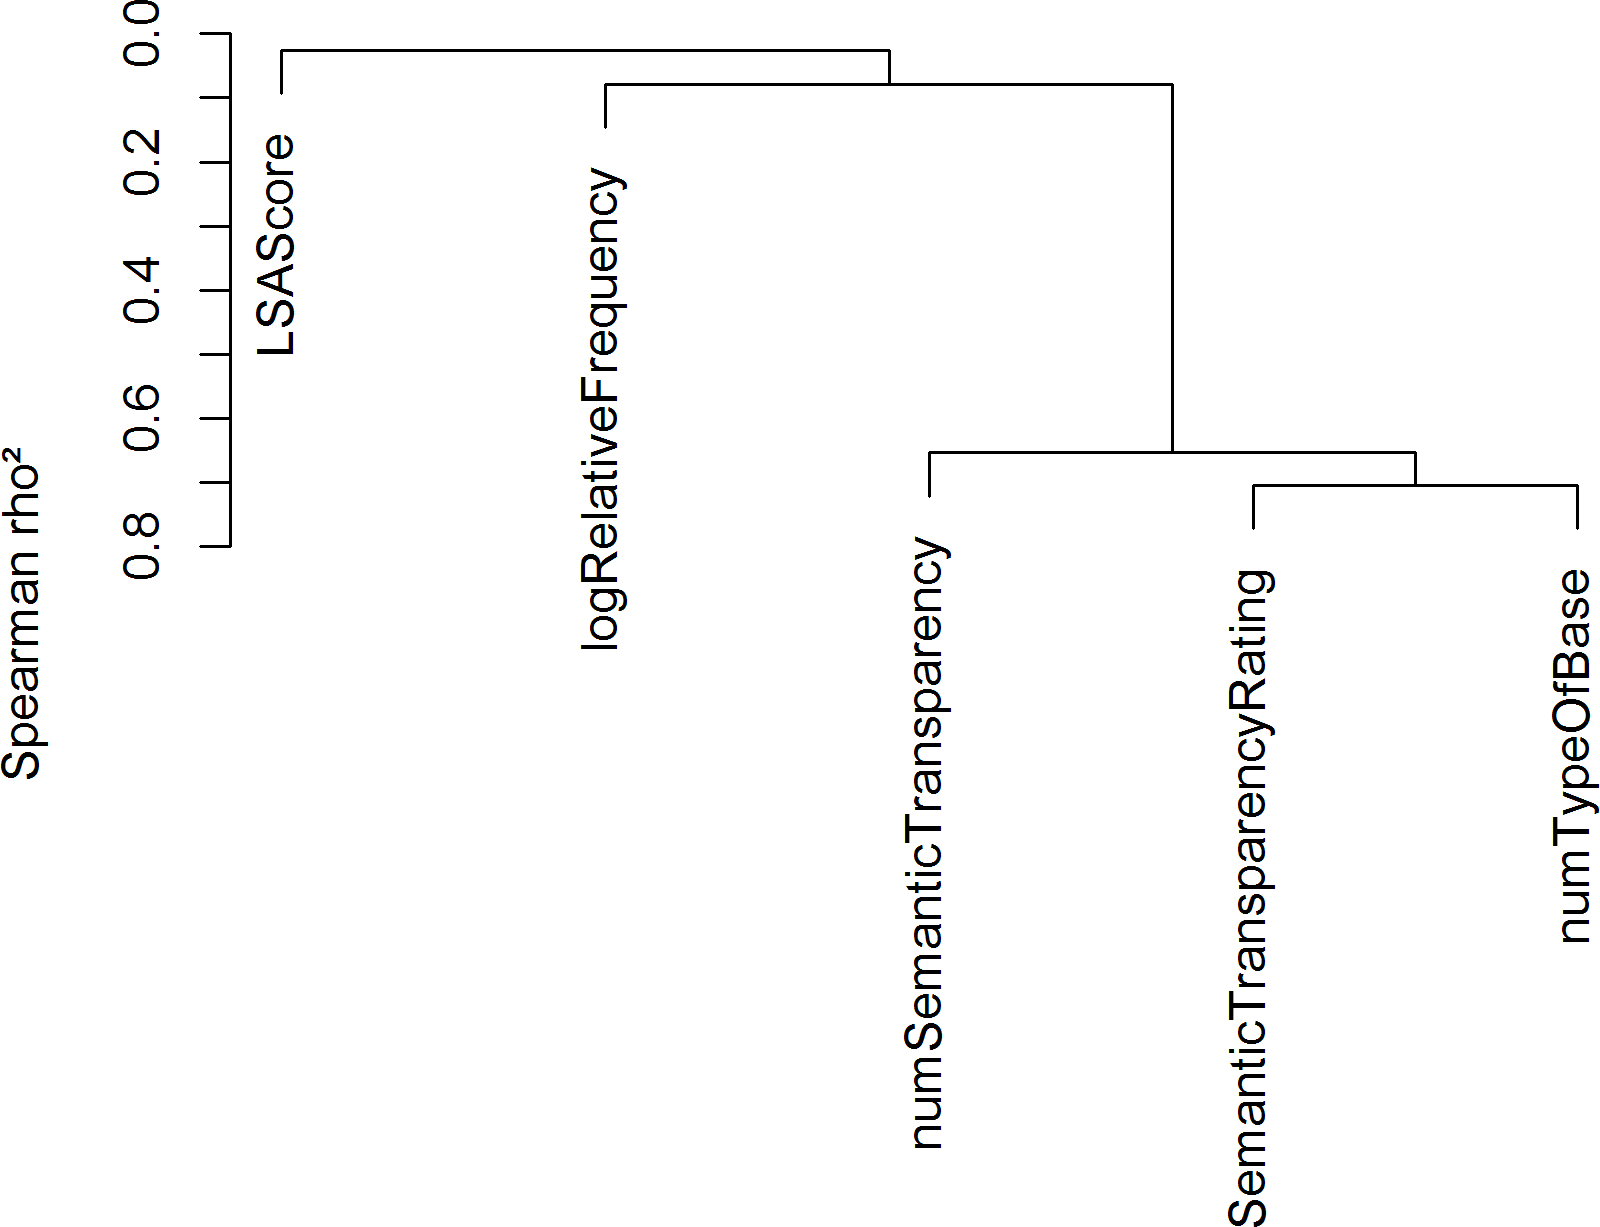
\includegraphics[scale=0.5]{images/Corpus/clusterAnalysisDecomposabilityCorpusAllTypes.png}
    	\caption{ Dendrogram of the five decomposability measures for all types in the corpus study}
    	\label{fig:cluster corpus all affixes}
    \end{figure*}
      
      
  The third split is the one splitting \textsc{numSemanticTransparency} from \textsc{Seman-ticTransparencyRating} and \textsc{numTypeOfBase}. This split is displayed in the lower part of the figure, which indicates that even though  \textsc{SemanticTrans-parencyRating} and \textsc{numTypeOfBase} are more similar to each other than they are to \textsc{numSemanticTransparency}, all three variables correlate to a high degree and are very similar.
  
 
 Let us now turn to the analyses of the individual affixes.
 It turned out that fitting a \is{hierarchical cluster analysis}{cluster analysis} was only reasonable for the prefixes \is{in-}\prefix{in} and \is{dis-}\prefix{dis}, i.e. it was not reasonable to conduct \is{hierarchical cluster analysis}{cluster analyses} for \is{un-}\prefix{un} and \is{-ly}\suffix{ly}. 
 This is due to the distribution of the \is{decomposability measure}decomposability variables in the \is{un-}\prefix{un} and the \is{-ly}\suffix{ly}-data sets. Three of the five \is{decomposability measure}decomposability variables do not show enough variability to be investigated. All of the \is{un-}\prefix{un} and \textit{ly-}affixed words are \is{semantic transparency}semantically transparent, and only a few feature a bound root. Furthermore, all \is{un-}\prefix{un}prefixed, and the majority of \is{-ly}\suffix{ly}-suffixed words were rated as very decomposable. Because of this lack of variability in the variables \textsc{SemanticTransparency}, \textsc{SemanticTransparencyRating} and \textsc{TypeOfBase}, only the correlation between log\textsc{RelativeFrequency} and \textsc{LSAScore} was investigated for \is{un-}\prefix{un} and \is{-ly}\suffix{ly}.
 The squared Spearman correlation score is below 0.05 for all correlations tested. This means there is no indication that the two variables log\textsc{RelativeFrequency} and \textsc{LSAScore} can be used as the operationalization of the same concept.
 
 
 
 
 
 For \is{in-}\prefix{in} and \is{dis-}\prefix{dis}, all variables showed enough variation to conduct \is{hierarchical cluster analysis}{cluster analyses}. The results of the analyses for the two prefixes are displayed in the dendrograms in \figref{fig:cluster corpus dis and in}. 
 For both prefixes, the variables \textsc{numSemanticTransparency}, \textsc{SemanticTransparency-Rating} and \textsc{numTypeOfBase} cluster together in the lower part of the figure. This means that the correlations between the three variables are quite high. \textsc{LSAScore} and log\textsc{RelativeFrequency}, on the other hand, do not correlate to a high degree with any other variable. This resembles the results of the first \is{hierarchical cluster analysis}{cluster analysis}.

\begin{figure*}  
	
	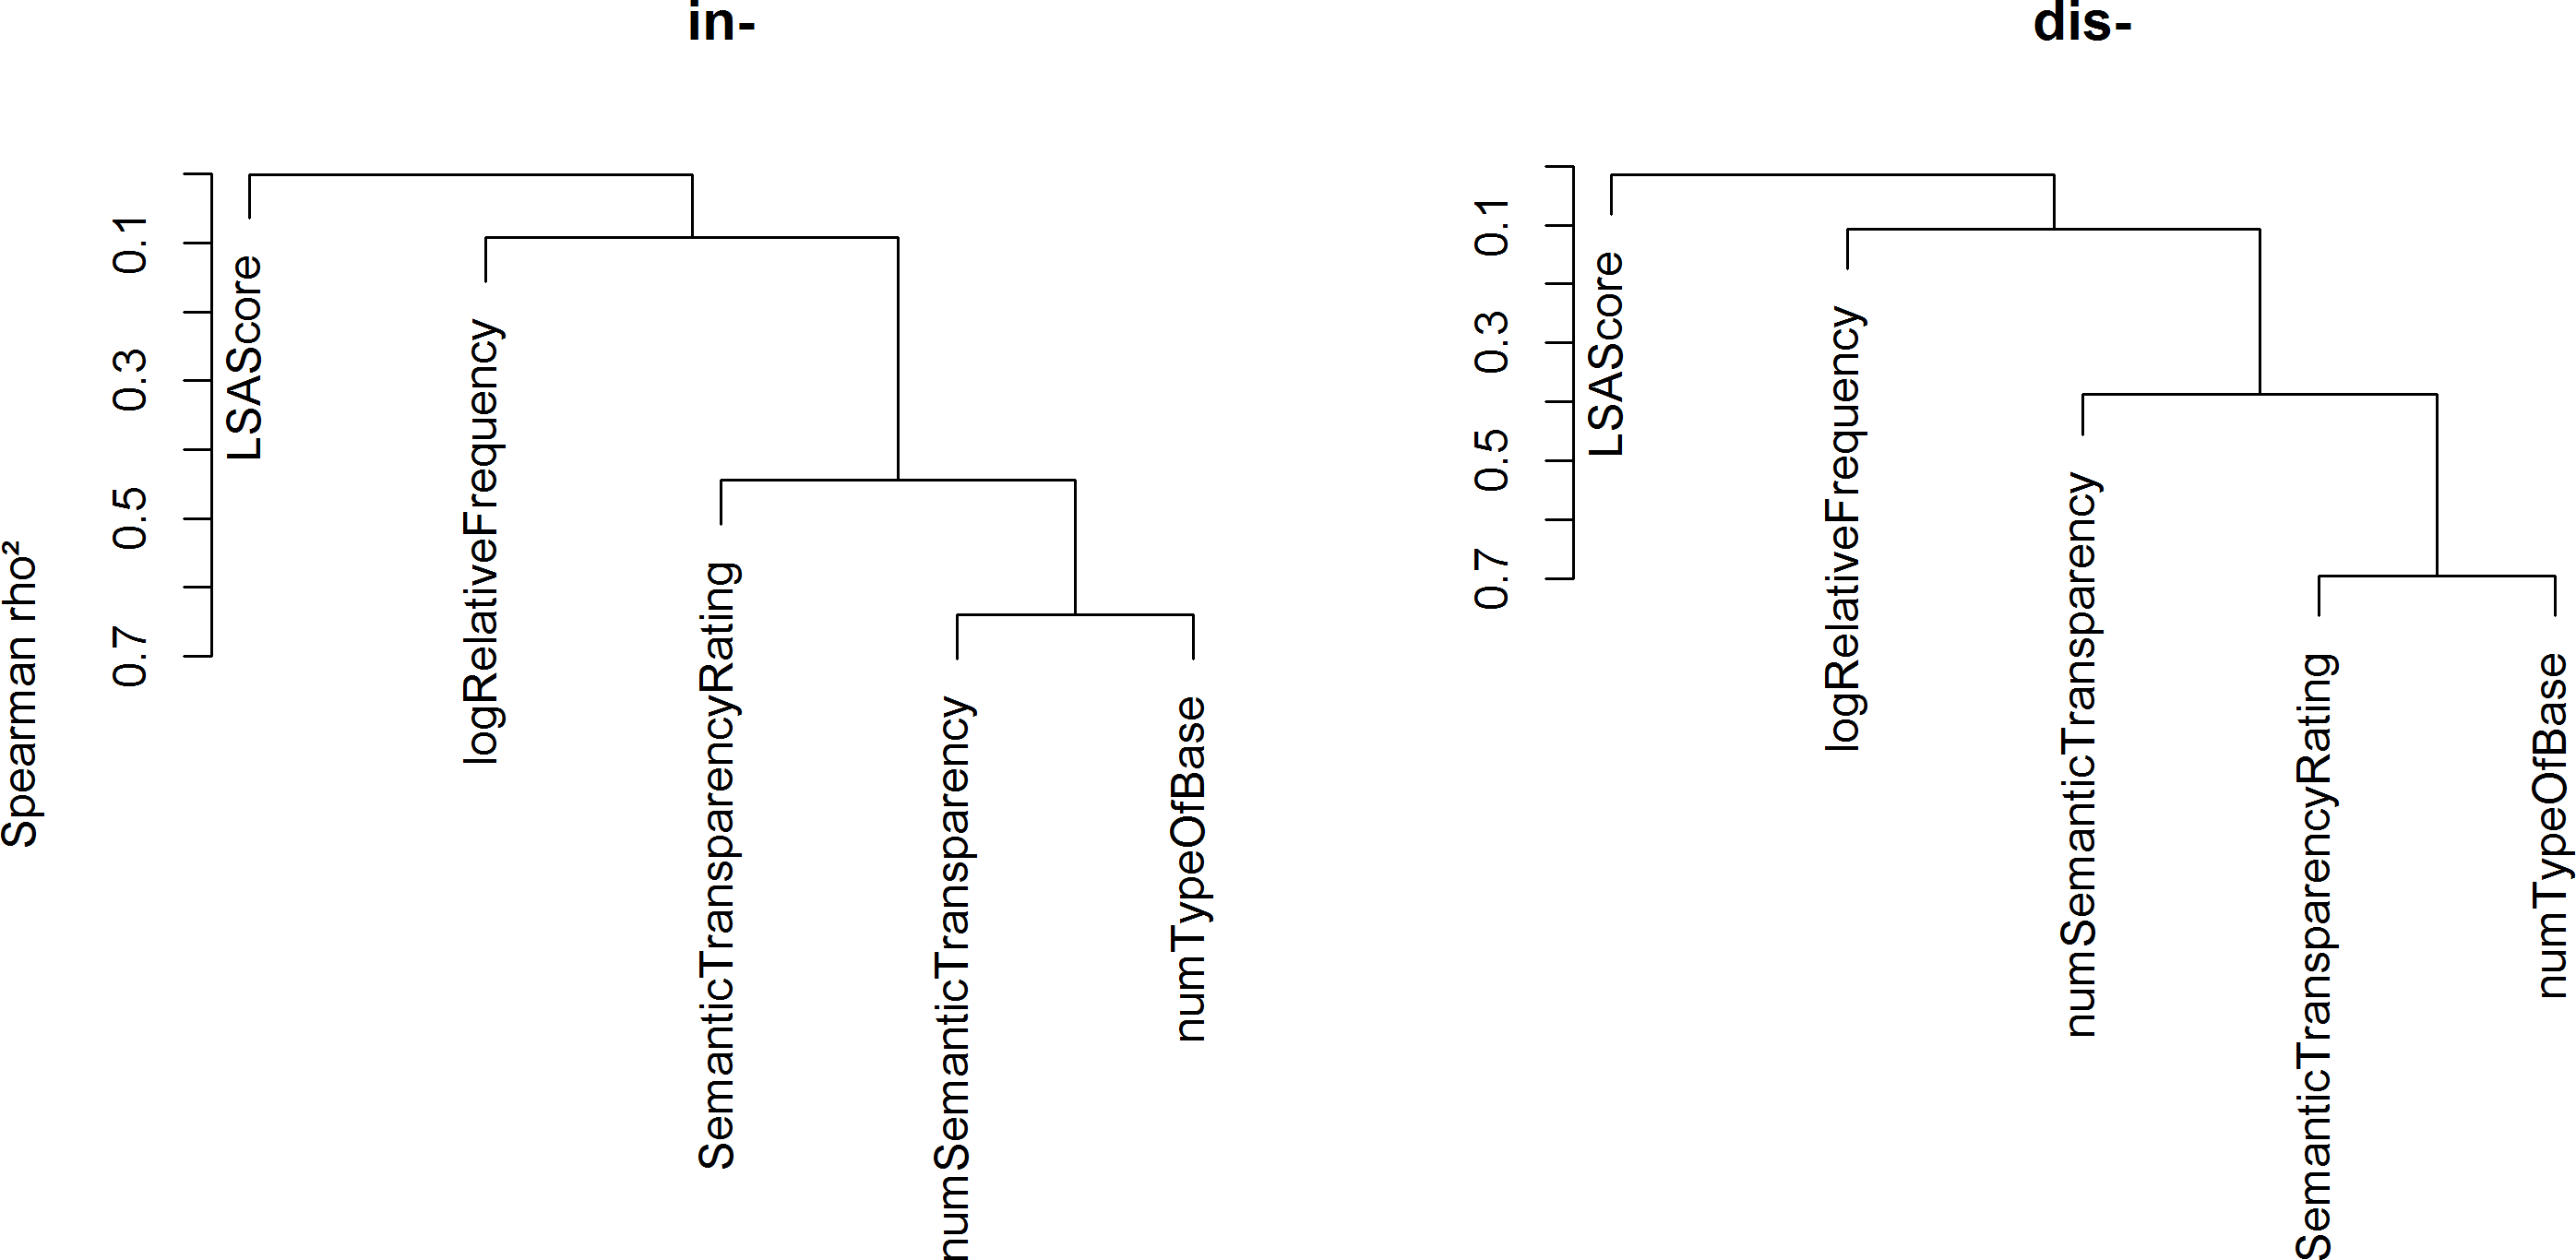
\includegraphics[scale=0.5]{images/Corpus/clusterAnalysisDecomposabilityCorpusDisAndIn.png}
	\caption{ Dendrogram of the five decomposability measures for \prefix{in} and \prefix{dis}prefixed words in the corpus study}
	\label{fig:cluster corpus dis and in}
\end{figure*}



To sum up, the \is{hierarchical cluster analysis}{cluster analyses} have revealed that the three variables \textsc{Semantic-Transparency}, \textsc{SemanticTransparencyRating} and \textsc{TypeOfBase} are highly correlated. The two variables log\textsc{RelativeFrequency} and \textsc{LSAScore}, in contrast, barely correlate with the other \is{decomposability measure}decomposability variables.
These outcomes can be interpreted in the following way: while the three variables  \textsc{SemanticTransparency}, \textsc{SemanticTransparencyRating} and \textsc{TypeOfBase} can certainly be used as measures of the same concept, this cannot be stated for the two variables log\textsc{RelativeFrequency} and \textsc{LSAScore}. In other words,  while possible effects of \textsc{SemanticTransparency}, \textsc{SemanticTransparencyRating} and \textsc{TypeOfBase} on duration are probably caused by the same underlying property, any effects of log\textsc{RelativeFrequency} and \textsc{LSAScore} can be regarded as independent.


The result that only three of the five investigated variables are measuring the same underlying property, i.e. that two measures are independent, raises the question of which variable, or which set of variables, is the right measure of \isi{decomposability}.
The answer to this question is not trivial and depends on one's definition of the concept \newterm{decomposability}. As thoroughly discussed in \sectref{decomposability}, \isi{decomposability} is not explicitly defined in the literature and different operationalizations are used. In other words, \isi{decomposability} is not one uniform theoretical concept and cannot be treated as such. Different operationalizations call for different definitions of the concept. 
The analyses conducted in this section indicate that the \is{decomposability measure}decomposability measures used in this study form operationalizations of three different types of \isi{decomposability}. The first type is operationalized by \textsc{SemanticTransparency}, \textsc{TypeOfBase} and \textsc{SemanticTransparencyRating}, the second is operationalized by log\textsc{RelativeFrequency}, and the third is operationalized by \textsc{LSAScore}.
The answer to the question of which variable measures \isi{decomposability} is thus that all five variables are measures of \isi{decomposability} but that they do not measure the same type of \isi{decomposability}. 

 

\subsection{The segmentability of the affixes: A comparison}
\label{The decomposability of the four affixes: a comparison}

Two of the theoretical predictions about \is{morphological gemination}{gemination}, i.e. the affix-specific \is{segmentability}morphological segmentability prediction and the affix-specific \is{informativeness}morphological informativeness prediction (cf. \sectref{decomposability}), are based on the lexical \isi{segmentability} hierarchies proposed in \sectref{comparison affixes}. To ensure the validity of these predictions, it is necessary to ensure the validity of the proposed \isi{segmentability} hierarchies (see \figref{fig:Segmentability hierarchies of  affixes repetition 2} for a repetition of the hierarchies). 
The Semantic Segmentability Hierarchy is mainly based on a qualitative analysis of the affixes' semantics (see discussion on semantics of the affixes in \sectref{comparison affixes}). Testing its validity by a quantitative analysis, such as the one applied here, is therefore quite challenging.
 The validity of the Non-Semantic Segmentability Hierarchy can, however, well be tested by checking whether the hierarchy is mirrored in the distribution of the \is{decomposability measure}decomposability measures in this data set.
 
 



\begin{figure*}
		
	
\begin{tabularx}{\linewidth}{lll}
	
	& \textbf{Segmentability}&	\textbf{Additional 	}  		  \\
	
	&	\textbf{hierarchy	}	&		\textbf{assumption }  	  \\		
	\midrule\\
	
	\textbf{Semantic} & \prefix{un} > \{\prefix{dis}, \prefix{in}\textsubscript{\textsc{Neg}}\}>  \prefix{in}\textsubscript{\textsc{Loc}} > \suffix{ly}& lexical meaning over pro-	 		  \\	
	\textbf{Hierarchy}	& & ductivity, transparency and 	 		  \\	
	& & type of base			 		  \\	
	\\
	\textbf{Non-Semantic}	&  	\prefix{un} > \suffix{ly} > \{\prefix{dis}, \prefix{in}\textsubscript{\textsc{Neg}}\}>  \prefix{in}\textsubscript{\textsc{Loc}}&		 \isi{productivity}, transparency			   \\	
	\textbf{Hierarchy}& & and  type of base	over   \\	
	& & lexical meaning		  		  \\	
	\midrule \\						
\end{tabularx}

	
	\caption{Lexical segmentability hierarchies of  affixes}
	\label{fig:Segmentability hierarchies of  affixes repetition 2} 
	
\end{figure*}


I tested the validity of the Non-Semantic Segmentability Hierarchy by comparing the \isi{segmentability} of the five investigated affixes as found in the data. I looked at the distributions of the \is{decomposability measure}decomposability variables\footnote{Note that I will continue to use the term \textit{{decomposability} measures} for the five variables \textsc{SemanticTransparency}, \textsc{SemanticTransparencyRating}, \textsc{TypeOfBase}, log\textsc{RelativeFrequency} and \textsc{LSAScore}, even though the results of the \is{hierarchical cluster analysis}{cluster analyses} have revealed that these variables do not form measures of the same underlying property. I will continue to use the term \is{decomposability measure}{\textit{decomposability variables}} because of two reasons. First, to avoid confusion. The term is used in the literature as well as \sectref{General Method} of this book to refer to these variables, and it might cause confusion to change the terminology at this point. Second, even though the variables might not measure the same underlying property, it can still be argued that they all form operationalizations of \isi{decomposability}. Importantly, \isi{decomposability} has to be defined in different terms depending on the \isi{decomposability} measure used.} for each affix in the data set, and used standard test statistics, such as the $\chi$-square-test and the Kruskal-Wallis test, to see whether differences between affixes were statistically significant.
If the Non-Semantic Segmentability Hierarchy is valid, the comparison should reveal the same \isi{segmentability} hierarchy  as the one proposed. 


First, I looked at the distribution of the variable \textsc{SemanticTransparency} for each affix. The distribution is shown in \tabref{tbl:Corpus distribution semantic transparency}. The table shows how many types of each affix were classified as semantically opaque, and how many were classified as \is{semantic transparency}semantically transparent. The percentage of opaque and transparent types per affix is given in parentheses next to the total number of  types. The more transparent types an affix features, the more segmentable it is. The affixes are ordered from the least to the most segmentable.




\begin{table*}
	\caption{Semantic Transparency by affix }
	\label{tbl:Corpus distribution semantic transparency}
	
	\resizebox{\textwidth}{!}{%
		\begin{tabular} {lrrrrrrrrrr}
			
			
			\lsptoprule
			\textsc{Semantic}& & & &&   \\
			\textsc{Transparency }&\multicolumn{2}{c}{\prefix{in}\textsubscript{\textsc{Loc}}   }&\multicolumn{2}{c}  {\textit{dis-}} &   \multicolumn{2}{c} {\prefix{in}\textsubscript{\textsc{Neg}}   } &\multicolumn{2}{c} {\prefix{un} }& \multicolumn{2}{c} {\suffix{ly}  }  \\
			\midrule
			
			opaque              &     42 &(78\%) &   28 &(45\%)    &  7& (24\%) & 0 &(0\%)   & 0 & (0\%)      \\
			transparent  &  12& (22\%)  &   34& (55\%) &  22 &(76\%)  & 101 &(100\%)  & 150  &(100\%) \\
			\lspbottomrule                                                                                
		\end{tabular}
	}

	
\end{table*}



The affixes \is{un-}\prefix{un} and \is{-ly}\suffix{ly} only feature transparent items, i.e. they are the semantically most transparent affixes out of the five. They are followed by \is{negative in-}negative \prefix{in} and \is{dis-}\prefix{dis}. Locative \prefix{in} has the most opaque items and is thus the least segmentable affix in terms of \isi{semantic transparency}.
 A $\chi$-square-test ($\chi$-$squared=204.48$, $df=4$, $p$ $< 0.001$) and  pairwise comparisons of proportions (see, for example, \citealt[chapter 6.5]{Crawley.2012}) revealed that the contrasts between all affixes are significant (except for the one between \is{un-}\prefix{un} and \is{-ly}\suffix{ly}).



The distribution of the variable \textsc{SemanticTransparencyRating} reveals a similar picture. \tabref{tbl:Corpus distribution semantic transparency rating} shows the distribution of the median ratings (of types) for each affix. Again, the total number of types and the percentage of types are given. 
The two affixes \prefix{un} and \is{-ly}\suffix{ly} were rated to be the easiest to segment. Locative \prefix{in} and \is{dis-}\prefix{dis} were rated to be the most difficult to segment.
 


\begin{table*}

	\caption{Semantic Transparency Rating  by affix }
	\label{tbl:Corpus distribution semantic transparency rating}

	
	\resizebox{\textwidth}{!}{%
				\begin{tabular} {lrrrrrrrrrr}
			
			
			\lsptoprule
			\textsc{Semantic}& & & &&   \\
			\textsc{TransparencyRating }&\multicolumn{2}{c}{\prefix{in}\textsubscript{\textsc{Loc}}   }&\multicolumn{2}{c}  {\textit{dis-}} &   \multicolumn{2}{c} {\prefix{in}\textsubscript{\textsc{Neg}}   } & \multicolumn{2}{c} {\suffix{ly}  } &\multicolumn{2}{c} {\prefix{un} }  \\
			\midrule
			
			1 - most decomposable             &     2 & 4\%) &   40 & (65\%)    &  20&  (69\%)   & 145&  (97\%)  & 101&  (100\%)        \\
			2                                                            &  13 & (24\%) &   4 & (6\%) &  1 & (3\%)&   4 & (2\%)& 0 & (0\%)  \\
			3															 &  25 & (46\%) &   14 &  (23\%)&  4&  (14\%) & 1 & (1\%) &0 & (0\%)    \\
			4 -  least decomposable             &  14&  (26\%) &   4 & (6\%) &  4 & (14\%) & 0 & (0\%) & 0 & (0\%)   \\
			\lspbottomrule                                                                                
		\end{tabular}
}

	
\end{table*}




To test whether the differences between affixes were significant, pairwise Krus-kal-Wallis tests were applied.  Only a few differences proved to be significant. The ratings for \is{locative in-}locative \prefix{in} differ significantly from the ratings for all other affixes. Furthermore, the ratings for \is{dis-}\prefix{dis} differ significantly from the ratings for \is{un-}\prefix{un} and \is{-ly}\suffix{ly}. 
One can thus say that there is a significant difference between the affixes which were rated as the most difficult to segment (\prefix{in}\textsubscript{\textsc{Loc}} and \is{dis-}\prefix{dis}) and the affixes which were rated as being the most easy to segment (\is{un-}\prefix{un} and \is{-ly}\suffix{ly}). However, due to the small size of the tested data sets combined with the rather high number of levels ( i.e. 4 levels for each affix) and the differences in number of observations between affixes, one must be cautions to not over-interpret the significance, or insignificance, of the contrasts. 
All in all, the rating clearly shows that \is{locative in-}locative \prefix{in} is the least segmentable affix, and that \is{un-}\prefix{un} and \is{-ly}\suffix{ly} are the most segmentable affixes.



\tabref{tbl:Corpus distribution type of base} gives the distribution for the variable \textsc{TypeOfBase} for all affixes. It shows that \is{locative in-}locative \prefix{in}, unlike all other affixes, has a strong preference for bound roots. Almost all of the \is{un-}\prefix{un} and \is{-ly}\suffix{ly}-affixed words feature a word as a base. For \is{negative in-}negative \prefix{in} and \is{dis-}\prefix{dis}, there are quite a few words which feature a bound root. As indicated by pairwise tests of proportions, the differences between all affixes, except for the one between \is{un-}\prefix{un} and \is{-ly}\suffix{ly} and the one between \is{negative in-}negative \prefix{in} and \is{dis-}\prefix{dis}, are significant. On can thus state that in terms of type of base, \is{locative in-}locative \prefix{in} is the least segmentable affix, \is{un-}\prefix{un} and \is{-ly}\suffix{ly} are the most segmentable affixes, and \is{dis-}\prefix{dis} and \is{negative in-}negative \prefix{in} pattern in between.

\begin{table}
	\caption{Type of base by affix}
	\label{tbl:Corpus distribution type of base}
	
	\resizebox{\textwidth}{!}{%
		\begin{tabular} {lrrrrrrrrrr}
			
			
			\lsptoprule
			\textsc{TypeOf}& & & &&   \\
			\textsc{Base }&\multicolumn{2}{c}{\prefix{in}\textsubscript{\textsc{Loc}}   }&\multicolumn{2}{c}  {\textit{dis-}} &   \multicolumn{2}{c} {\prefix{in}\textsubscript{\textsc{Neg}}   } &\multicolumn{2}{c} {\is{un-}\prefix{un} }& \multicolumn{2}{c} {\suffix{ly}  }  \\
			\midrule
			
			bound root            &     44 &  (81\%) &   15 &  (24\%)  &  7 &  (24\%)  & 1 &  (1\%)   & 1&  (1\%)        \\
			word          & 10 &  (19\%) &  47 &  (76\%) &  22 &  (76\%)   & 100&   (99\%)   & 149&   (99\%)  \\
			\lspbottomrule                                                                                
		\end{tabular}
	}

	
\end{table}



Turning to the gradient measures of \isi{decomposability}, \figref{fig: corpus RelFreq comparison} displays the distribution of the variable log\textsc{RelativeFrequency} 
for the five affixes using boxplots. The logarithmized \isi{relative frequency} is displayed on the x-axis of the plot.  Each of the five boxes in the plot represents 50\% of the types of one affix.  The black dot in each box marks the median \isi{relative frequency} for each affix. For example, the graph shows that 50\% of the \is{-ly}\suffix{ly}-words have a logarithmized \isi{relative frequency} between $-2.191$ and $-0.058$. It also shows that half of the \is{-ly}\suffix{ly}-words have a \isi{relative frequency} above $-1.415$, and half have a \isi{relative frequency} below $-1.415$. All significant differences are indicated in the plot.


\begin{figure*}  
	
	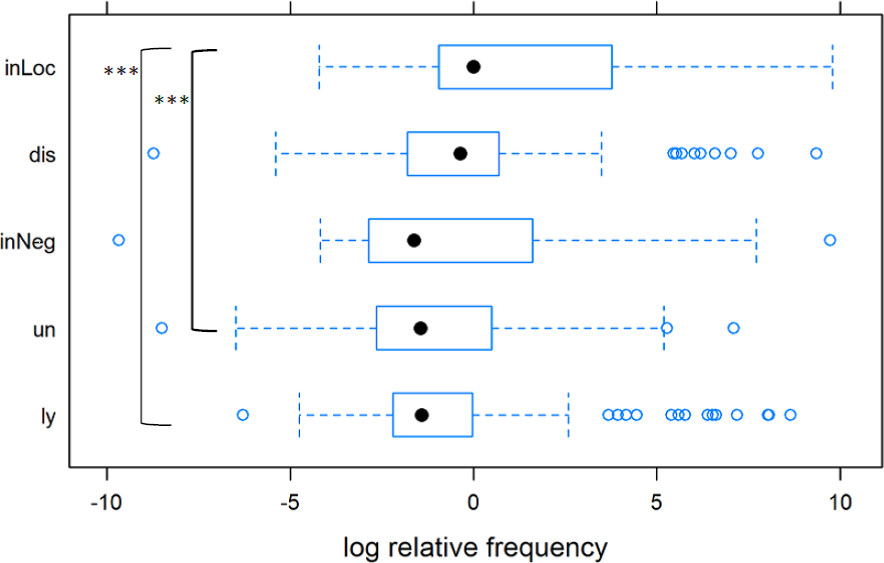
\includegraphics[scale=0.5]{images/Corpus/corpusComparisonRelFreq2.png}
	\caption{ Comparison of the relative frequency of the five affixes }
	\label{fig: corpus RelFreq comparison}

\end{figure*}


The plot suggests that \is{locative in-}locative \prefix{in} is the least segmentable affix having the highest \isi{relative frequency}. It is followed by \is{dis-}\prefix{dis}. The median relative {frequencies} of \is{in-}\prefix{in}, \is{un-}\prefix{un} and \is{-ly}\suffix{ly} do not differ to a high degree, but the plot suggests that, with regard to their \isi{decomposability}, \is{-ly}\suffix{ly} and \is{un-}\prefix{un}affixed words are more uniform than words with \is{negative in-}negative \prefix{in}. In other words, while the majority of the \is{-ly}\suffix{ly}- and \is{un-}\prefix{un}words have a rather low \isi{relative frequency}, we find some variation with \is{negative in-}negative \prefix{in}. 
 An ANOVA ($F=6.716 ,p<0.001$) indicates that there is a significant difference between the \isi{relative frequency} of the five affixes. Pairwise comparisons using Tukey contrasts reveal, however, that only two of the differences are significant. The affix with the highest \isi{relative frequency}, \is{locative in-}locative \prefix{in}, is significantly different from the two affixes with the lowest \isi{relative frequency}, \is{un-}\prefix{un} ($t$-$value=4.813, p<0.001$)  and \is{-ly}\suffix{ly} ($t$-$value=4.489, p<0.001$). 

            

One reason for the insignificance of the contrasts between the affixes might be that there are not enough observations for each affix to reach significance. Furthermore, the differences in \isi{relative frequency} between the affixes are quite small. This is partly due to the gradient nature of the variable log\textsc{RelativeFre-quency}. In combination, the size of the data set and the gradient nature of the variable might lead to a lack of statistical power. 
To alleviate this problem, I recoded the variable log\textsc{RelativeFrequency} into a categorical one. This especially makes sense considering that the variable has a natural threshold. For all types with a \isi{relative frequency} below 0, the derivative is less frequent than its base. For all items having a \isi{relative frequency} higher than 0, the opposite is the case. Therefore, items with a \isi{relative frequency} below 0 were recoded as being \textit{more decomposable}, and items with a \isi{relative frequency} higher than 0 were recoded as \textit{less decomposable }(see \citealt{Hay.2001,Collie.2008} for a similar coding of \isi{relative frequency}). \tabref{tbl:Corpus Categorical RelFreq} displays the distribution across affixes.
Pairwise comparisons revealed that \is{-ly}\suffix{ly} has significantly more {more decomposable} words  than \is{negative in-}negative \prefix{in}, \is{locative in-}locative \prefix{in} and \is{dis-}\prefix{dis}. Furthermore, \is{locative in-}locative \prefix{in} has significantly less {more decomposable} words than \is{un-}\prefix{un} and \is{negative in-}negative \prefix{in}. 







% Summary Rel Freq
To sum up the comparisons of the affixes' \isi{relative frequency}, \is{un-}\prefix{un} and \is{-ly}\suffix{ly} are the most segmentable affixes, \is{locative in-}locative \prefix{in} is the least segmentable affix. The affixes \is{dis-}\prefix{dis} and \is{negative in-}negative \prefix{in} seem to be in the middle of the scale. However, in both analyses (gradient and categorical \isi{relative frequency}), only few contrasts proved to be significant.






\begin{table*}
	
	\caption{Categorical relative frequency by affix }
	\label{tbl:Corpus Categorical RelFreq}
	
		\resizebox{\textwidth}{!}{%
			\begin{tabular} {lrrrrrrrrrr}
				\lsptoprule
				\textsc{Cat. Relative}& & & &&   \\
				\textsc{Frequency }&\multicolumn{2}{c}{\prefix{in}\textsubscript{\textsc{Loc}}   }&\multicolumn{2}{c}  {\textit{dis-}} &   \multicolumn{2}{c} {\prefix{in}\textsubscript{\textsc{Neg}}   } &\multicolumn{2}{c} {\prefix{un} }& \multicolumn{2}{c} {\suffix{ly}  }  \\
				\midrule
				less    decomposable              &     38 &(70\%) &   30 &(48\%)   &  9 &(31\%)  & 35& (35\%)   &35& (23\%)        \\
				more decomposable &  16 &(30\%) &   32& (52\%)  &  20 &(69\%) &66& (65\%) & 115& (77\%) \\
				\lspbottomrule                                                                                
		\end{tabular}
		}
	
\end{table*}




\begin{figure*}
	
	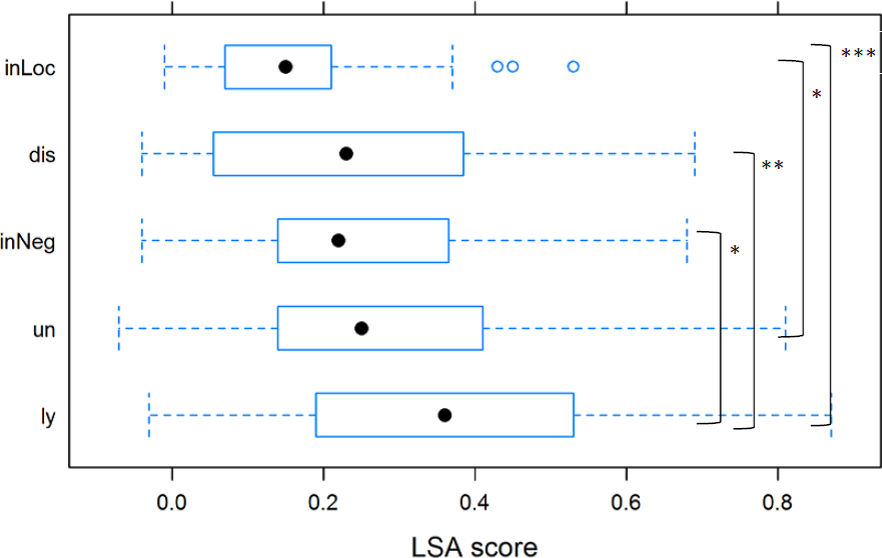
\includegraphics[scale=0.5]{images/Corpus/corpusComparisonLSAScores2.png}
	\caption{ Comparison of LSA score of the five affixes }
	\label{fig: corpus LSA comparison}
\end{figure*}


%  LSA
Turning to the last measure of \isi{decomposability}, the comparison of the affixes' \is{Latent Semantic Analysis (LSA)}LSA scores reveals that there are only minor differences between the affixes. \figref{fig: corpus LSA comparison} displays these differences using boxplots. On the x-axis the \is{Latent Semantic Analysis (LSA)}LSA score is displayed. Each box represents the distribution of the \is{Latent Semantic Analysis (LSA)}LSA scores for one affix in increasing order. Locative \prefix{in} has the lowest score indicating that words featuring this affix are the least semantically similar to their base words. In terms of {semantic similarity}, they can thus be said to be the least decomposable words in the data set. Words with the affix \is{-ly}\suffix{ly} have the highest score, and are thus the most similar to their base word. They are the most decomposable.
However, the figure shows that there is a big overlap in the distribution of the \is{Latent Semantic Analysis (LSA)}LSA scores across affixes, i.e. the differences between affixes are rather small. Statistical analyses confirm this impression.
While an ANOVA ($F=8.512, p< 0.001$) showed a significant effect of the affix on the \is{Latent Semantic Analysis (LSA)}LSA score, the pair-wise comparison of the means using Tukey contrasts shows  that only four of the contrasts are significant. The affix \is{-ly}\suffix{ly} has significantly higher \is{Latent Semantic Analysis (LSA)}LSA scores than the affixes \is{un-}\prefix{un} ($t$-$value=0.027, p=0.01$), \is{locative in-}locative \prefix{in} ($t$-$value=5.197, p< 0.001$) and \is{dis-}\prefix{dis}  ($t$-$value=3.443, p=0.006$). Furthermore, the affix \is{un-}\prefix{un} has significantly higher scores than the  affix \is{locative in-}locative \prefix{in} ($t$-$value=2.772, p=0.044$). 



        When interpreting the results for the variable \textsc{LSAScore}, it should be remembered that for some affixes not all items were taken into consideration in the comparisons. While for most of the \is{-ly}\suffix{ly}- and \is{un-}\prefix{un}affixed words the \is{Latent Semantic Analysis (LSA)}LSA score could be computed (118 types for \is{-ly}\suffix{ly}, 89 types for \is{un-}\prefix{un}), for the other affixes fewer types were considered in this comparison (between 23 and 40). Therefore, it is not surprising that we only find significant contrasts with \is{-ly}\suffix{ly} and \is{un-}\prefix{un}, but not with the other affixes.  
        
        One can summarize that despite the fact that for a lot of types no \is{Latent Semantic Analysis (LSA)}LSA score could be computed, and the comparison of affixes in terms of their \is{Latent Semantic Analysis (LSA)}LSA score is thus based on a rather small number of observations, the distribution of the variable \textsc{LSAScore} reveals the same picture as the other \is{decomposability measure}decomposability variables. Locative \prefix{in} is the least segmentable affix, followed by \is{dis-}\prefix{dis} and \is{negative in-}negative \prefix{in}. The affixes \is{un-}\prefix{un} and \is{-ly}\suffix{ly} are the most segmentable affixes. 
        
                                                               
After having looked at each \isi{decomposability} measure individually, let us now take a look at the whole picture. \tabref{tbl:summary comparison of affix} summarizes the results of the comparisons by showing a \isi{segmentability} hierarchy for each \isi{decomposability} measure. The \isi{segmentability} hierarchies rank the affixes from the most segmentable to the least segmentable. The table shows very similar hierarchies for all measures. Locative \prefix{in} is the least segmentable affix, followed by \is{dis-}\prefix{dis} and \is{negative in-}negative \prefix{in}. The affixes \is{un-}\prefix{un} and \is{-ly}\suffix{ly} are the most segmentable affixes out of the five. 


\begin{table*}
	\caption{Segmentability hierarchies for each decomposability measure}
	\label{tbl:summary comparison of affix}
	
			\resizebox{\textwidth}{!}{%
		\begin{tabular} {lrcrcrcrcr}
			\lsptoprule
			\textbf{Decomposability measure}& & &&&&& &&\\
			\midrule
			\textsc{SemanticTransparency}  &\{\prefix{un} &, &\suffix{ly}\}  &>&   \prefix{in}\textsubscript{\textsc{Neg}}  &>&  \prefix{dis}  &>&\prefix{in}\textsubscript{\textsc{Loc}}  \\		
			
			\textsc{SemanticTransparencyRating }&\prefix{un}  &>& \suffix{ly}  &>&   \prefix{in}\textsubscript{\textsc{Neg}}   &>&\prefix{dis}  &>&  \prefix{in}\textsubscript{\textsc{Loc}}  \\	
			
			\textsc{TypeOfBase} &\{\prefix{un} &, &\suffix{ly}\}  &>&   \{\prefix{in}\textsubscript{\textsc{Neg}}  &,&  \prefix{dis}\}  &>&\prefix{in}\textsubscript{\textsc{Loc}}  \\	
			
			log\textsc{RelativeFrequency}&\suffix{ly} &> &  \prefix{un}  &> &   \prefix{in}\textsubscript{\textsc{Neg}}&> &  \prefix{dis}     &> &\prefix{in}\textsubscript{\textsc{Loc}}  \\				
			
			\textsc{Cat.RelativeFrequency}&\suffix{ly} &> &  \prefix{un}  &> &   \prefix{in}\textsubscript{\textsc{Neg}}&> &  \prefix{dis}     &> &\prefix{in}\textsubscript{\textsc{Loc}}  \\				
			
			\textsc{LSAScore}&\suffix{ly} &> &  \prefix{un}  &> &   \prefix{in}\textsubscript{\textsc{Neg}}&> &  \prefix{dis}     &> &\prefix{in}\textsubscript{\textsc{Loc}}  \\				
			
			\lspbottomrule                                                                                
		\end{tabular}
	}
	
\end{table*}



The differences  between the hierarchies mostly concern the ranking of \is{un-}\prefix{un} and \is{-ly}\suffix{ly}. In terms of \textsc{LSAScore} and log\textsc{RelativeFrequency}, \is{-ly}\suffix{ly} is more segmentable than \is{un-}\prefix{un}, in terms of \textsc{SemanticTransparencyRating}, \is{un-}\prefix{un} is more segmentable than \is{-ly}\suffix{ly}, and in terms of \textsc{SemanticTransparency} and \textsc{TypeOfBase}, there is no difference between the two. 
While all hierarchies display a very similar picture, it is to note that they differ with regard to how significant differences between affixes are. While for \textsc{SemanticTransparency} and \textsc{TypeOfBase} all differences were significant, this was not the case for the other measures of \isi{decomposability}. 


The results of the \isi{segmentability} comparison fit in with previous research on the \isi{segmentability} of prefixes. \cite{Zirkel.2010}, for example, investigated the parsability of 15 prefixes in terms of four different measures (\isi{productivity}, type parsing ratio, token parsing ratio and average \isi{boundary strength}). The comparison of the prefixes revealed that out of the 15 investigated prefixes, \is{un-}\prefix{un} is the third most segmentable, and \is{dis-}\prefix{dis} is the 10th most segmentable. In other words, as in the present study, the prefix \is{un-}\prefix{un} is very segmentable and the prefix \is{dis-}\prefix{dis} is far less segmentable. The prefix \is{in-}\prefix{in} was not investigated in \cite{Zirkel.2010}. 

Overall, the \isi{segmentability} hierarchies displayed in \tabref{tbl:summary comparison of affix} match the Non-Semantic Segmentability Hierarchy. Thus, the Non-Semantic Segmentability Hierarchy is borne out by the data. This supports its validity and thus shows that the predictions made by the affix-specific Morphological Segmentability Approach are valid.

\subsection{Summary } \label{summary decomposability corpus study}

% Cluster analyses
In the first part of this section the relation between the five measures of \isi{decomposability} \textsc{SemanticTransparency}, \textsc{SemanticTransparencyRating}, \textsc{TypeOfBase}, log\textsc{RelativeFrequency} and \textsc{LSAScore} was investigated. The \is{hierarchical cluster analysis}{cluster analyses} revealed that the three variables \textsc{SemanticTransparency}, \textsc{SemanticTrans-parencyRating} and \textsc{TypeOfBase} are highly correlated. The two gradient measures  log\textsc{RelativeFrequency} and \textsc{LSAScore}  did not correlate with any other \isi{decomposability} variable.  
One can thus summarize that, while  \textsc{SemanticTransparency}, \textsc{SemanticTransparencyRating} and \textsc{TypeOfBase} tap into the same phenomenon, and are therefore well suited to be used as operationalizations of the same concept, this cannot be said for 
log\textsc{RelativeFrequency} and \textsc{LSAScore}. 
It was argued that the results can be interpreted as evidence for three different types of \isi{decomposability}. The first type is operationalized by  \textsc{SemanticTransparency}, \textsc{SemanticTransparencyRating} and \textsc{TypeOfBase}, the second by log-\textsc{RelativeFrequency}, and the third by \textsc{LSAScore}. Potential effects of the \is{decomposability measure}decomposability variables must be interpreted with these different types of \isi{decomposability} in mind. 

 In the second part of the section, the distributions of the \is{decomposability measure}decomposability variables across affixes were compared. All comparisons revealed the same picture. Locative \prefix{in} is the least segmentable affix, \is{un-}\prefix{un} and \is{-ly}\suffix{ly} are the most segmentable. The prefixes \is{negative in-}negative \prefix{in} and \is{dis-}\prefix{dis} pattern in between. 
 Even though not all contrasts proved to be significant, and the categorical measures seemed to provide a clearer picture than the gradient measures, one can say that the decline in \isi{segmentability} from \is{un-}\prefix{un} and \is{-ly}\suffix{ly} to \is{locative in-}locative \prefix{in} is supported by all measures. 
 This order resembles the Non-Semantic Segmentability Hierarchy (cf. \figref{fig:Segmentability hierarchies of  affixes repetition 2} ). The corpus data thus empirically verifies one of the proposed \isi{segmentability} hierarchies. In turn, the \isi{gemination} prediction of the affix-specific Segmentability Approach, which is based on the Non-Semantic Segmentability Hierarchy, is valid. 

\section{Duration}


\subsection{Analyses} \label{analyses dur corpus}


The first durational analysis consists of investigating the distribution of consonant duration in each subset to test whether \isi{gemination} is a categorical or a gradient phenomenon (cf. `Nature of \isi{gemination}: Predictions' in \sectref{predictions nature of gemination}). To see whether the distributions significantly differ between environments, I generated boxplots for each environment of each subset and applied standard test statistics. 
If doubles show a significantly higher mean than singletons, and the boxplots indicate that the distributions of doubles and singles differ significantly, the data shows a bimodal distribution. In that case, one can assume \isi{gemination} to be categorical. 
If there is no significant difference in the distribution of the environments, two explanations are possible. The first one is that the \is{morphological gemination}morphological geminates in the given data set \is{degemination}{degeminate}, i.e. there is no difference in the duration of doubles and singles in the data set. The other possibility is that {gemination} is a gradient phenomenon which is not traceable by merely looking at distributions of durations and comparing averages. To check which of the two explanations holds, further statistical models are needed, i.e. linear \is{regression model}{regression models}. 



I fitted at least two linear \is{regression model}{regression models} for each subset, one predicting \is{absolute duration}absolute consonant duration in milliseconds  (\textsc{AbsoluteConsonantDuration}) and one predicting relative consonant duration (\textsc{RelativeConsonantDuration}). Relative consonant duration refers to the duration of the consonant relative to the duration of the preceding vowel. In addition to the models for each subset, one model directly comparing the three prefixes with nasals, i.e. \is{un-}\prefix{un}, \is{locative in-}locative \prefix{in} and \is{negative in-}negative \prefix{in}, was fitted. While this model has the advantage of directly comparing the three prefixes with each other, it also faces several problems, such as the systematic difference in the distribution of variables between the prefixes. As will be discussed in the pertinent section, these problems limit the usefulness of the model to a great degree, e.g. some variables cannot be investigated in the model.

In the \isi{relative duration} models, the independent variable \textsc{PrecedingSegmentDuration} was not included. This was because \isi{relative duration} is computed by means of preceding segment duration. In other words, the variable \textsc{PrecedingSegmentDuration} is part of the dependent variable and therefore not a suitable predictor variable.


With regard to the \is{decomposability measure}decomposability measures, only in the \is{in-}\prefix{in} and \is{dis-}\prefix{dis}models all five \is{decomposability measure}decomposability variables were included. In the \is{un-}\prefix{un} and \is{-ly}\suffix{ly}-models, only the effects of log\textsc{RelativeFrequency} and \textsc{LSAScore} were tested. The reason is the distribution of the variables in the different subsets (see \sectref {The decomposability of the four affixes: a comparison} for discussion). 
Since the variable \textsc{LSAScore} was not coded for all items, i.e. the inclusion of the variable results in a loss of a lot of data points, the effect of this variable was tested individually in all subsets. 

In the models predicting consonant duration with \is{in-}\prefix{in} and \is{dis-}\prefix{dis}, \isi{collinearity} problems had to be addressed. As discussed in the previous section, the three \is{decomposability measure}decomposability variables \textsc{SemanticTransparency}, \textsc{SemanticTransparencyRating} and \textsc{TypeOfBase} highly correlate, and it was thus problematic to test all of them simultaneously in the model. Therefore, the effect of these variables was tested by including them individually in the model, and by conducting \is{principal component analysis}principal component analyses (cf. \sectref{stats}). 


The use of mixed effects models was precluded by the data's unnestedness. Almost every item is produced by a different speaker and many items occur only once in the corpus, so that it did not make sense to use speaker and item as random effects (see also discussion in \sectref{sampling corpus}). All models were fitted according to the modeling strategy described in \sectref{stats}.



All models were tested for two types of  interactions. First, I tested for interactions which are predicted to affect \is{morphological gemination}{gemination} according to the theoretical approaches discussed in Chapter \ref{Theory}. These  are the interactions between the variable \textsc{Environment} and the \is{decomposability measure}decomposability variables, and the interaction between \textsc{Environment} and \textsc{Affix}.
Then, I tested for interactions which, based on previous empirical work and theoretical considerations, can be assumed to affect affixational consonant duration. In other words, I tested for interactions between variables for which one can assume that their relationship leads to a situation in which the simultaneous influence of the variables on affixational consonant duration is not additive. One of those interactions is, for example, the interaction between \textsc{Environment} and \textsc{BaseInitialStress}. For prefixed words, it can be assumed that base-initial \isi{stress} affects the duration of a double consonant differently than the duration of a singleton. The reason is that, as discussed in \sectref{Phonological representation of geminates}, part of the double consonant belongs to the base-initial syllable, while the singleton only belongs to the prefix. 
Some interactions were not testable because some level combinations were not attested. An example of such an untestable interaction is the interaction between \textsc{Environment} and \textsc{BaseInitialStress} in the \is{un-}\prefix{un}data set. There are no \is{un-}\prefix{un}prefixed words with a double consonant and an unstressed base-initial syllable. All interactions tested in the corpus study are listed in \hyperref[Appendix C: Summaries of tested interactions in corpus study]{appendix C}.

After fitting the \is{regression model}{regression models} for each subset, I used \isi{multi-model inferencing} to verify the results, i.e. to ensure that \isi{multi-model inferencing} predicts the same variables to be important for predicting consonant duration as the final regression model (see \sectref{stats} for a discussion of \isi{multi-model inferencing}).




The plots of the \is{regression model}{regression models} were generated with the \texttt{visreg package} (\citealt{Breheny.2015}). For a plot showing the effect of a variable, all other variables are held constant at the median (for numeric variables) or at the most common category (for factors). For the models predicting \is{absolute duration}absolute consonant duration, the plots always show the response variable \textsc{AbsoluteNasalDuration} in milliseconds, i.e. in cases where the dependent variable had to be transformed in the modeling process, the plots show the back-transformed variable.



\subsection{Overview}\label{overview corpus}



\begin{figure*}[t!]
	
		
		
		\begin{subfigure}
			
			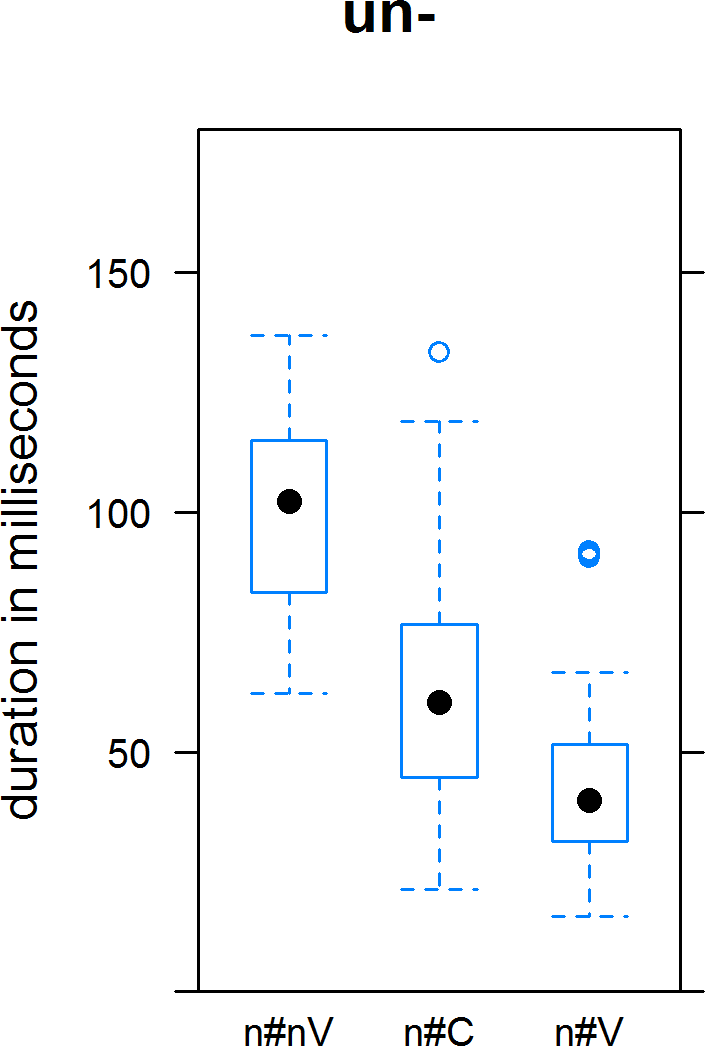
\includegraphics[scale=.55]{images/Corpus/boxUn.png}
			%	\caption{1a}
			%	\label{fig:sfig1}
		\end{subfigure}%
		~
		\begin{subfigure}
			
			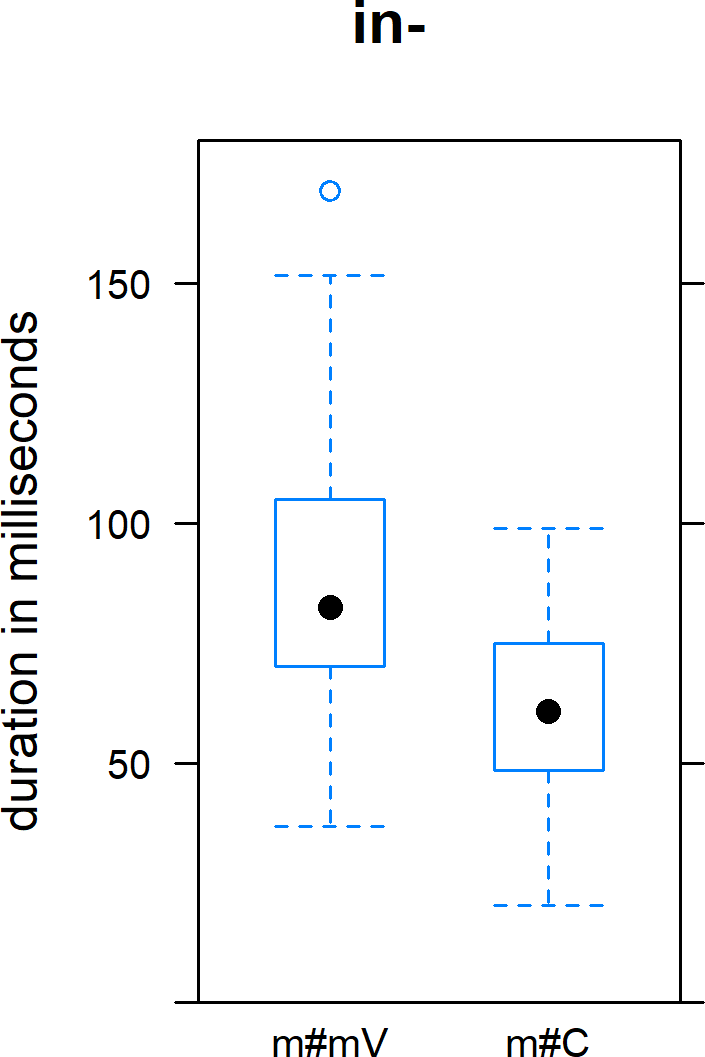
\includegraphics[scale=.55]{images/Corpus/boxIn.png}
			%	\caption{1b}
			%	\label{fig:sfig2}
		\end{subfigure}
		
		\begin{subfigure}
			
			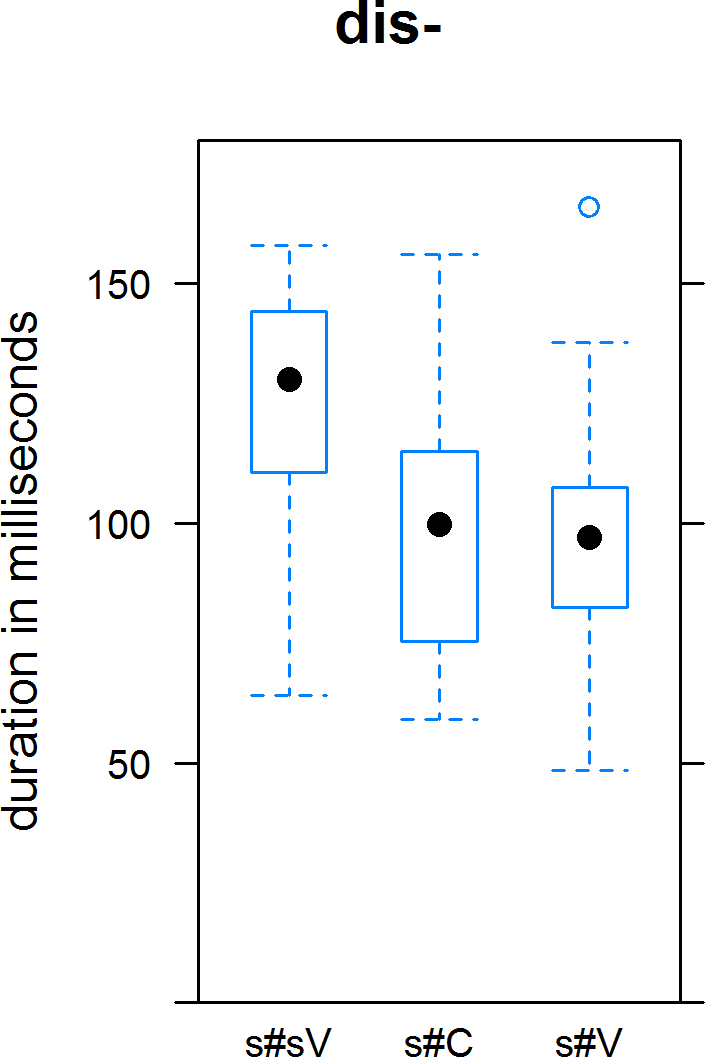
\includegraphics[scale=.55]{images/Corpus/boxDis.png}
			%	\caption{1b}
			%	\label{fig:sfig2}
		\end{subfigure}
		~
		\begin{subfigure}
			
			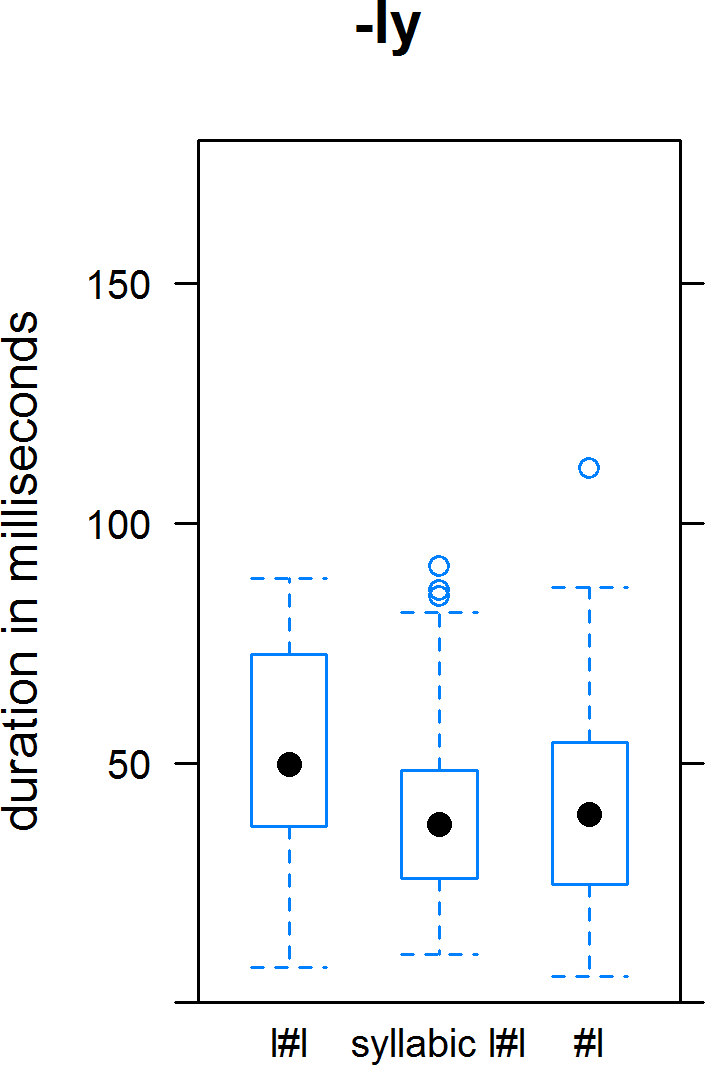
\includegraphics[scale=.55]{images/Corpus/boxLy.png}
			%	\caption{1b}
			%	\label{fig:sfig2}
		\end{subfigure}				
					
	\caption{Distribution of consonant duration in the four data sets}
	\label{fig:Corpus raw duration distribution}
\end{figure*}

% boxplots			
\figref{fig:Corpus raw duration distribution} depicts the distribution of consonant duration for each environment in each subset using boxplots. The distribution in the \is{un-}\prefix{un}data set is shown in the upper left panel, the one for \is{in-}\prefix{in} in the upper right panel, the one for \is{dis-}\prefix{dis} in the lower left panel, and the one for \is{-ly}\suffix{ly} in the lower right panel.
The y-axis of each plot displays the duration of the consonant in milliseconds. The leftmost box in each plot represents the distribution for items with a double consonant, and the boxes on the right show the distributions for items with a single consonant. For \is{-ly}\suffix{ly}, the box in the middle of the panel shows the distribution of the \is{syllabicity}syllabic doubles.
 
 
For the prefixes, the figure shows a clear difference in duration between double and single consonants. Doubles are longer than singletons. The figure also shows that there is a clear binary distribution in the \is{un-}\prefix{un}, \is{in-}\prefix{in} and \is{dis-}\prefix{dis}data sets.  For \is{in-}\prefix{in} and \is{dis-}\prefix{dis}, there is hardly any overlap in the interquartile range of doubles and singletons. For \is{un-}\prefix{un}, there is no overlap at all. For the prefixes, the durational distribution thus suggests a clear categorical difference between doubles and singletons. In other words, the plots suggest that the prefixes geminate, and that \isi{gemination} is a categorical phenomenon. 
The \is{-ly}\suffix{ly}-data set does not show a bimodal distribution, i.e. there is a big overlap in the distribution of doubles and singletons, and doubles are not significantly longer than singletons in this data set. One might thus suspect \isi{degemination} for \is{-ly}\suffix{ly}. Further statistical analyses are, however, necessary to confirm this impression.











  
  \begin{table*}
  	\caption{Duration of consonant(s) in milliseconds per environment for all affixes}
  	\label{tbl:Corpus raw duration}
  	
  		\begin{tabular} {lllll}
  			\lsptoprule
  			\textbf{un-}\\
  			%\\
  			Environment & Example & Mean & Median& Standard Deviation\\
  			\midrule			
  			n\#nV&\color{lsMidBlue}\textit{unnatural} & 100 & 102 & 21\\ 
  			n\#C&\color{lsMidBlue}\textit{untold} & 64 & 60 & 24\\ 
  			n\#V&\color{lsMidBlue}\textit{uneven} & 45 & 40 & 18\\
  			\midrule   	
  			Overall &  & 60 & 54 & 28\\ 
  			\midrule
  			%\midrule
  			\\
  			\textbf{in-}\\
  			%\\
  			
  			Environment & Example & Mean & Median& Standard Deviation\\
  			\midrule			
  			m\#mV&\color{lsMidBlue}\textit{immortal} & 87 & 81 & 27\\   	
  			m\#C&\color{lsMidBlue}\textit{impossible} & 61 & 61 & 19\\ 
  			\midrule   	
  			Overall &  & 76 & 74 & 27\\ 
  			\midrule   
  			%\midrule
  			\\
  			\textbf{dis-}\\
  			%\\
  			Environment & Example & Mean & Median& Standard Deviation\\
  			\midrule			
  			s\#sV&\color{lsMidBlue}\textit{dissatisfied} & 127 & 130  &35 \\ 
  			s\#C&\color{lsMidBlue}\textit{disgrace} & 100 & 100& 29\\ 
  			s\#V&\color{lsMidBlue}\textit{disarm} &95 & 96 & 22 \\ 
  			\midrule   	
  			Overall &   &103   & 102  & 30  \\ 
  			\midrule   	
  			%\midrule
  			\\
  			\textbf{-ly}\\
  			%\\
  			\midrule
  			Environment & Example & Mean & Median& Standard Deviation\\
  			\midrule			
  			l\#l&\color{lsMidBlue}\textit{really} & 50  & 50 & 23 \\ 
  			\is{syllabicity}syllabic l\#l&\color{lsMidBlue}\textit{ment(a)lly} &41 & 37  & 21\\ 
  			\#l&\color{lsMidBlue}\textit{possibly} & 42& 39& 21\\ 
  			\midrule   	
  			Overall &  &43  &41 &22\\ 
  			\lspbottomrule                                                                                
		\end{tabular}
  	
  \end{table*}
  

\tabref{tbl:Corpus raw duration} shows a summary of the distribution of consonant duration for each environment in the four subsets. Overall the durations of the consonants in the data set are in the same range as those found in other studies. For example, \citet[Tables II and X]{Umeda.1977} finds in her North American English data that intervocalic word-internal singleton /n/ is between 34 and 38 ms long (depending on \isi{stress}). 
Double /n/s across a word boundary have a duration of 100 ms. For singleton intervocalic word-medial /m/, Umeda finds mean durations between 70 and 74 ms, and for singleton /s/, mean durations range from 90 to 120 ms in that position. Singleton /l/ is between 40 and 47 ms long in Umeda's study. This indicates that the data and the durational measurements are valid.

Let us now turn to the distribution of duration for single and double consonants in the data, i.e. to the question of \isi{gemination}.  As already shown in \figref{fig:Corpus raw duration distribution}, for the three prefixes the mean and median duration of the double consonants is much higher than the mean and median duration of the single consonants. The differences in mean range from 26 ms (\texttt{m\#mV} to  \texttt{m\#C)} to 55 ms (\texttt{n\#nV} to  \texttt{n\#V}). For \is{-ly}\suffix{ly}, there is a difference in mean duration of 8 ms between double /l/ (\texttt{l\#l}) and single /l/ (\texttt{\#l}). The double is thus only slightly longer than the singleton.
  
  


% stats for doubles vs. singles

To get a first idea about the nature of these differences between environments, some univariate analyses were carried out. The pair-wise comparison of the means for \is{un-}\prefix{un} using Tukey contrasts yields significant contrasts for all three pairs, i.e. the differences between all environments are significant (see \tabref{tbl:Tukey un}). This suggests \isi{gemination} for \is{un-}\prefix{un}. 
For \is{in-}\prefix{in}, a Welch t-test shows a significant difference between the two environments \texttt{m\#mV} and \texttt{m\#C} ($t$($152.98$) $=7.1122$, $p< 0.001$). 
Thus, as in the \is{un-}\prefix{un}data set, in the \is{in-}\prefix{in}data set doubles are significantly longer than singletons.
For \is{dis-}\prefix{dis}, the comparison of the means also yields significant contrasts for the difference between doubles and singletons (see \tabref{tbl:Tukey dis}). However, the difference between the two singleton levels is not significant. None of the differences between the \is{-ly}\suffix{ly}-environments proved to be significant. Thus, while for all the prefixes, doubles are significantly longer than singletons, this is not the case for the suffix \is{-ly}\suffix{ly}.


  \begin{table*}
  	\caption{Multiple comparison of means of nasal duration for \prefix{un}prefixed words (Tukey contrasts)}
  	\label{tbl:Tukey un}
  	
  		\begin{tabular} {lrrrr}
			
			
			\lsptoprule
  			& Estimate & Std. Error & $t$-value  & Pr($>$$|$$t$$|$)    \\
  			\midrule
  			n\#C - n\#nV  &-35  &  5 & -6.903 & $<$ 0.001\\
  			n\#V - n\#nV & -56 &  5 & -10.798 & $<$ 0.001\\
  			n\#C - n\#V  & -20 & 4 & -5.487 & $<$ 0.001 \\
  			\lspbottomrule                                                                                
		\end{tabular}
  	
  \end{table*}
  
  
  
  \begin{table*}
  	\caption{Multiple comparison of means of consonant duration for \prefix{dis}prefixed words (Tukey contrasts)}
  	\label{tbl:Tukey dis}
  	
  		\begin{tabular} {lrrrr}
			
			
			\lsptoprule
  			& Estimate & Std. Error & $t$-value  & Pr($>$$|$$t$$|$)    \\
  			\midrule
  			s\#C - s\#sV  &  - 28 &  7  & -6.903 & 0.001\\
  			s\#V - s\#sV & -32  &  7  & -10.798 &$<$ 0.001\\
  			s\#C - s\#V    &  {5}       &  5  &  -0.858  &  0.666  \\
  			  			\lspbottomrule                                                                                
		\end{tabular}

  	
  \end{table*}
  
  

					

All in all, the first analyses of durations have shown that the singleton consonant durations in the data are similar to the ones found in previous studies and the data is thus valid. Furthermore, the investigation of distributions suggests that the investigated prefixes geminate and that \isi{gemination} is categorical. It also suggests \isi{degemination} for \is{-ly}\suffix{ly}. 
However, since it is well known that the duration of segments in \isi{natural speech} is subject to a variety of different influences, more advanced statistical analyses are necessary to investigate the matter. In the next subsections I will present such analyses for each subset.



\subsection{The prefix \prefix{un}} \label{un corpus}

\subsubsection{Absolute duration}

The \is{regression model}{linear model} predicting \isi{absolute duration} with \is{un-}\prefix{un} was fitted according to the procedure described in sections \ref{stats} and \ref{analyses dur corpus}. 
The residuals of the initial model showed a non-normal distribution. Therefore, the dependent variable \textsc{AbsolutConsonantDuration} was transformed by the Box-Cox-transformation parameter $0.303$, and outliers were removed. The removal of outliers resulted in the loss of  2 observations, i.e. 1.3\% of the observations. After the model was refitted with the transformed dependent variable, it showed a satisfactory distribution of residuals. The model was then simplified and interactions were tested  (see \hyperref[Appendix C: Summaries of tested interactions in corpus study]{appendix C} for a list of all tested interactions).
None of the interactions was significant, and only two significant predictors remained in the final model, \textsc{Environment} and  \textsc{LocalSpeechRate}. The model explains 57\% of the variance found in the data. \tabref{tbl: summary model un} documents the estimates for each predictor and their p-values in the final model.

\begin{table*}[!h]
	\caption{Summary of linear model for variables predicting the Box-Cox-transformed duration of [n] in \prefix{un}prefixed words}
	\label{tbl: summary model un}
	
		
		
		\begin{tabular}{lrrrr}
			
			
			\lsptoprule
			& Estimate & Std. Error & t-value & p-value  \\ 
			\midrule
			Intercept                           &   0.580 &  0.015  & 38.502 &  $<$ 0.001\\
			\textsc{Environment}-\texttt{n\#C} & -0.050 &  0.010 & -5.072 & $<$ 0.001\\
			\textsc{Environment}-\texttt{n\#V} & -0.097 &   0.010 & -9.770 & $<$ 0.001\\
			\textsc{LocalSpeechRate} &                 -0.008  & 0.001 &  -6.814 & $<$ 0.001\\
			
			\midrule\\
			Adjusted R-squared: 0.562  \\
			\lspbottomrule
		\end{tabular}

	
\end{table*}


\figref{fig:SpeechRate un} depicts the effect of \textsc{LocalSpeechRate}.  The y-axis of the graph displays the duration of the nasal in milliseconds, the horizontal axis represents the local \isi{speech rate}. The line represents the estimated effect of the variable. The shaded areas in the graphs represent the 95\% confidence intervals. The  plot shows, the higher the \isi{speech rate}, i.e. the more segments are pronounced in a given amount of time, the shorter becomes the nasal. This is an expected effect.





\begin{figure*}
	

	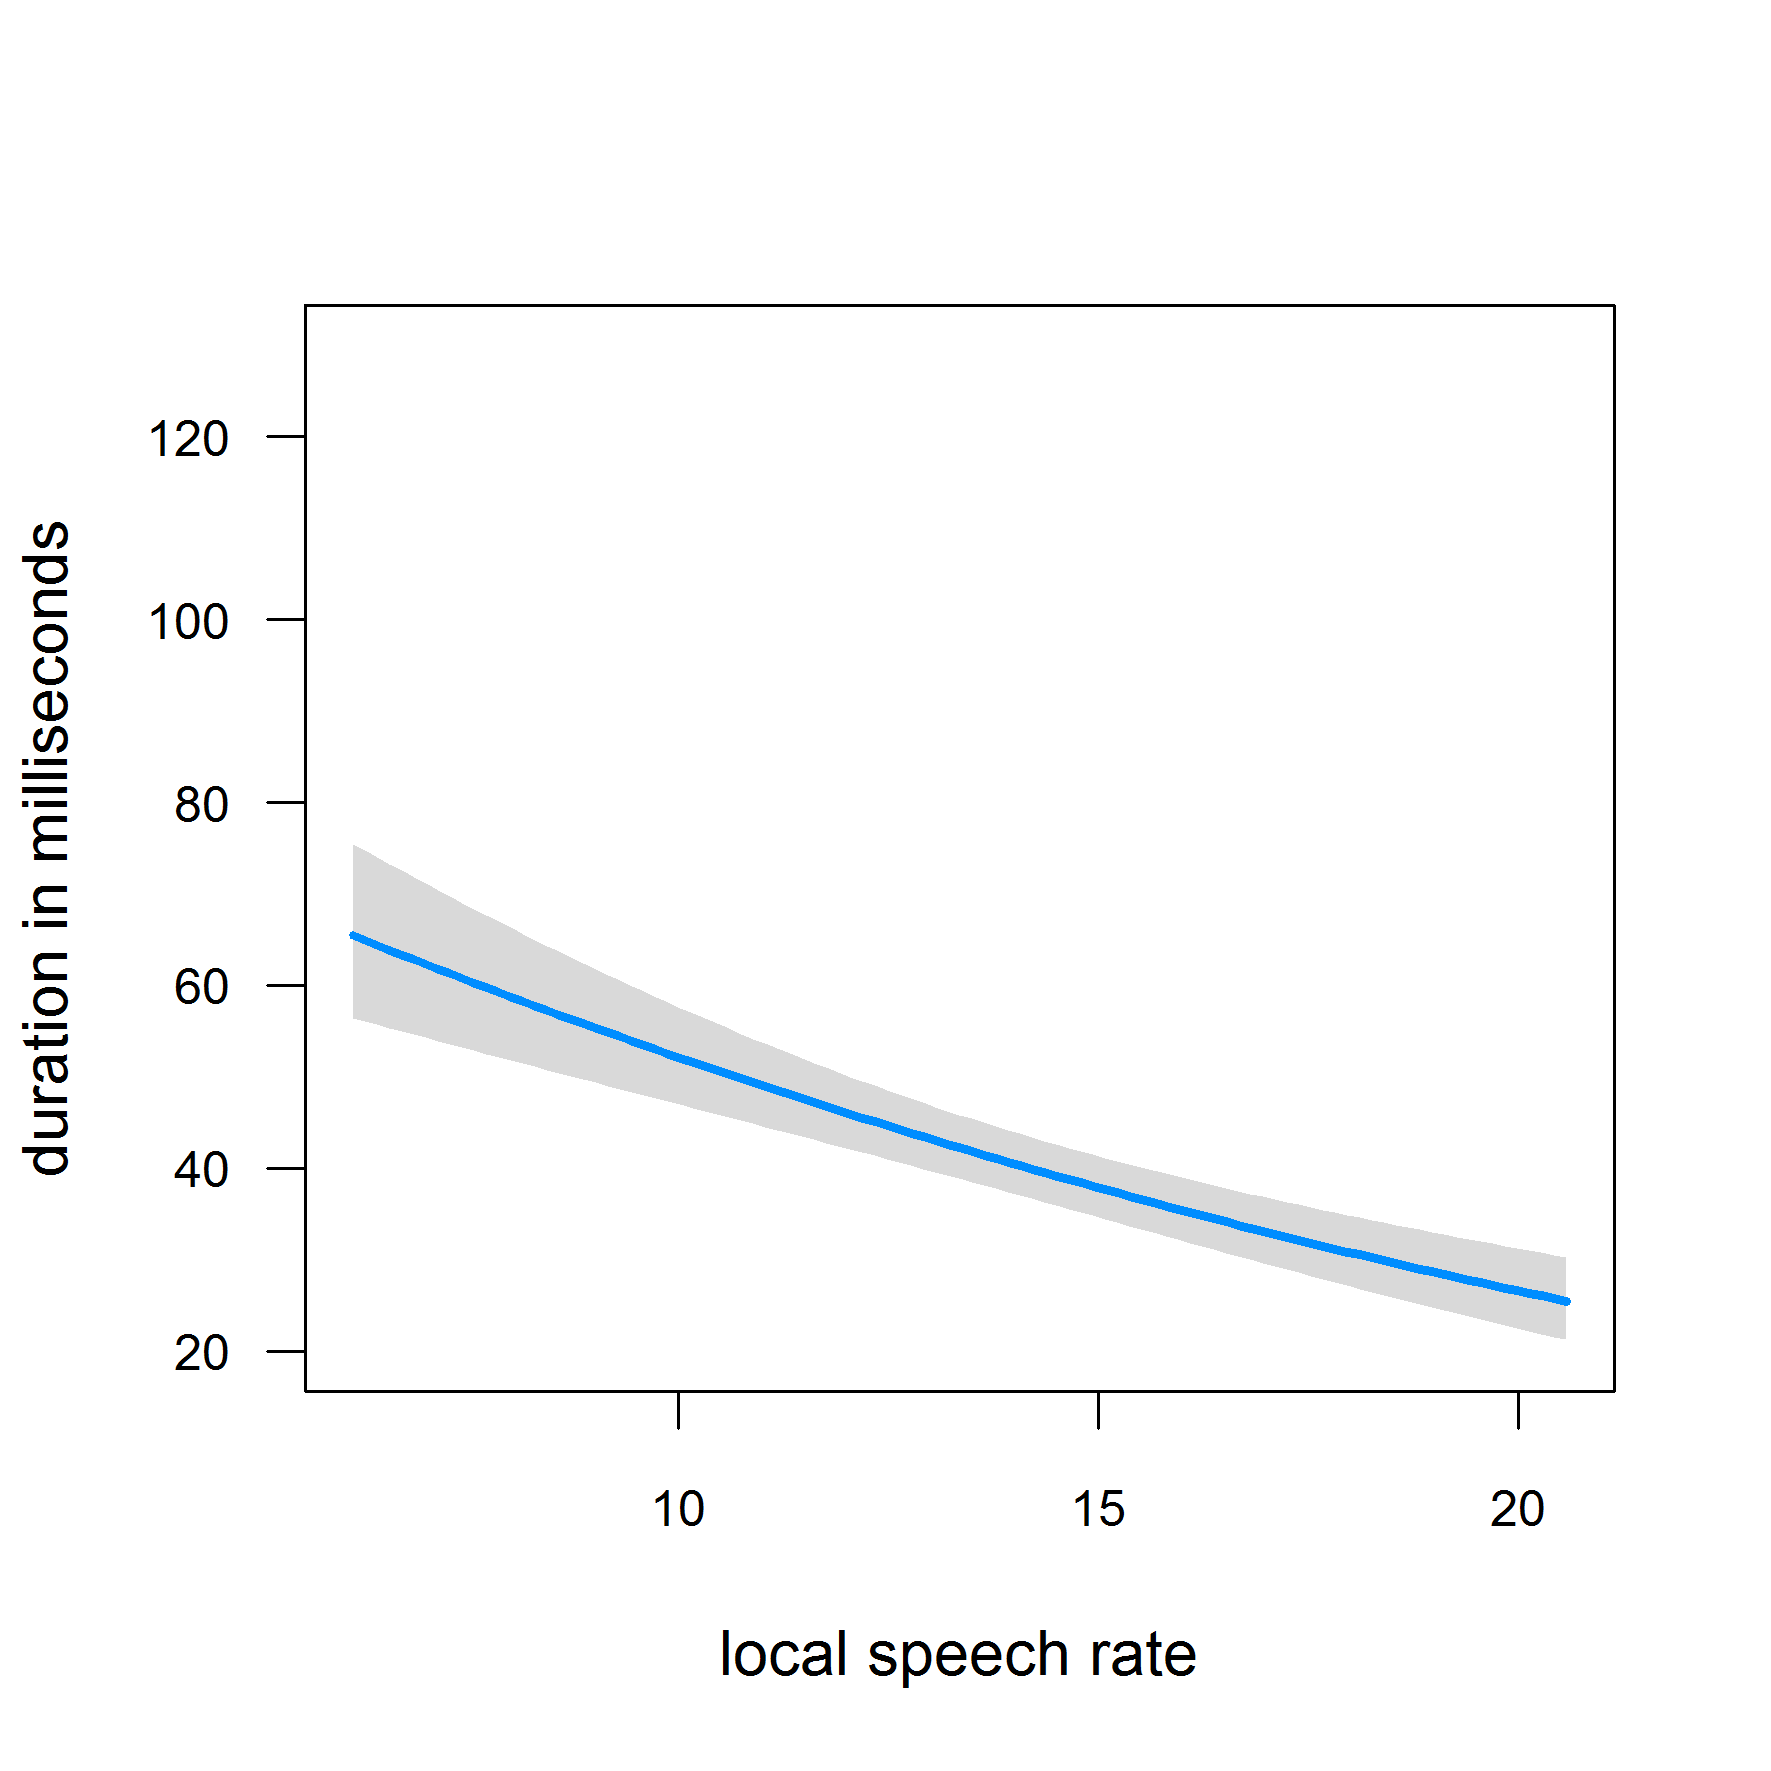
\includegraphics [scale=0.4]{images/Corpus/unModelSpeechRate.png}
	\caption{ Effect of local speech rate on consonant duration in \prefix{un}data set}
	\label{fig:SpeechRate un}

\end{figure*}





Let us now turn to our variable of interest, \textsc{Environment}. Its effect is shown in \figref{fig:NumNasal un}. The blue lines in the figure represent the estimated consonant duration for each of the three investigated environments. The graph shows that words containing a double nasal have a significantly longer duration than words with one nasal, no matter whether the single nasal is followed by a non-nasal consonant or by a vowel. In the case of a following vowel, the single /n/ is shortest. 




\begin{figure}  
	
	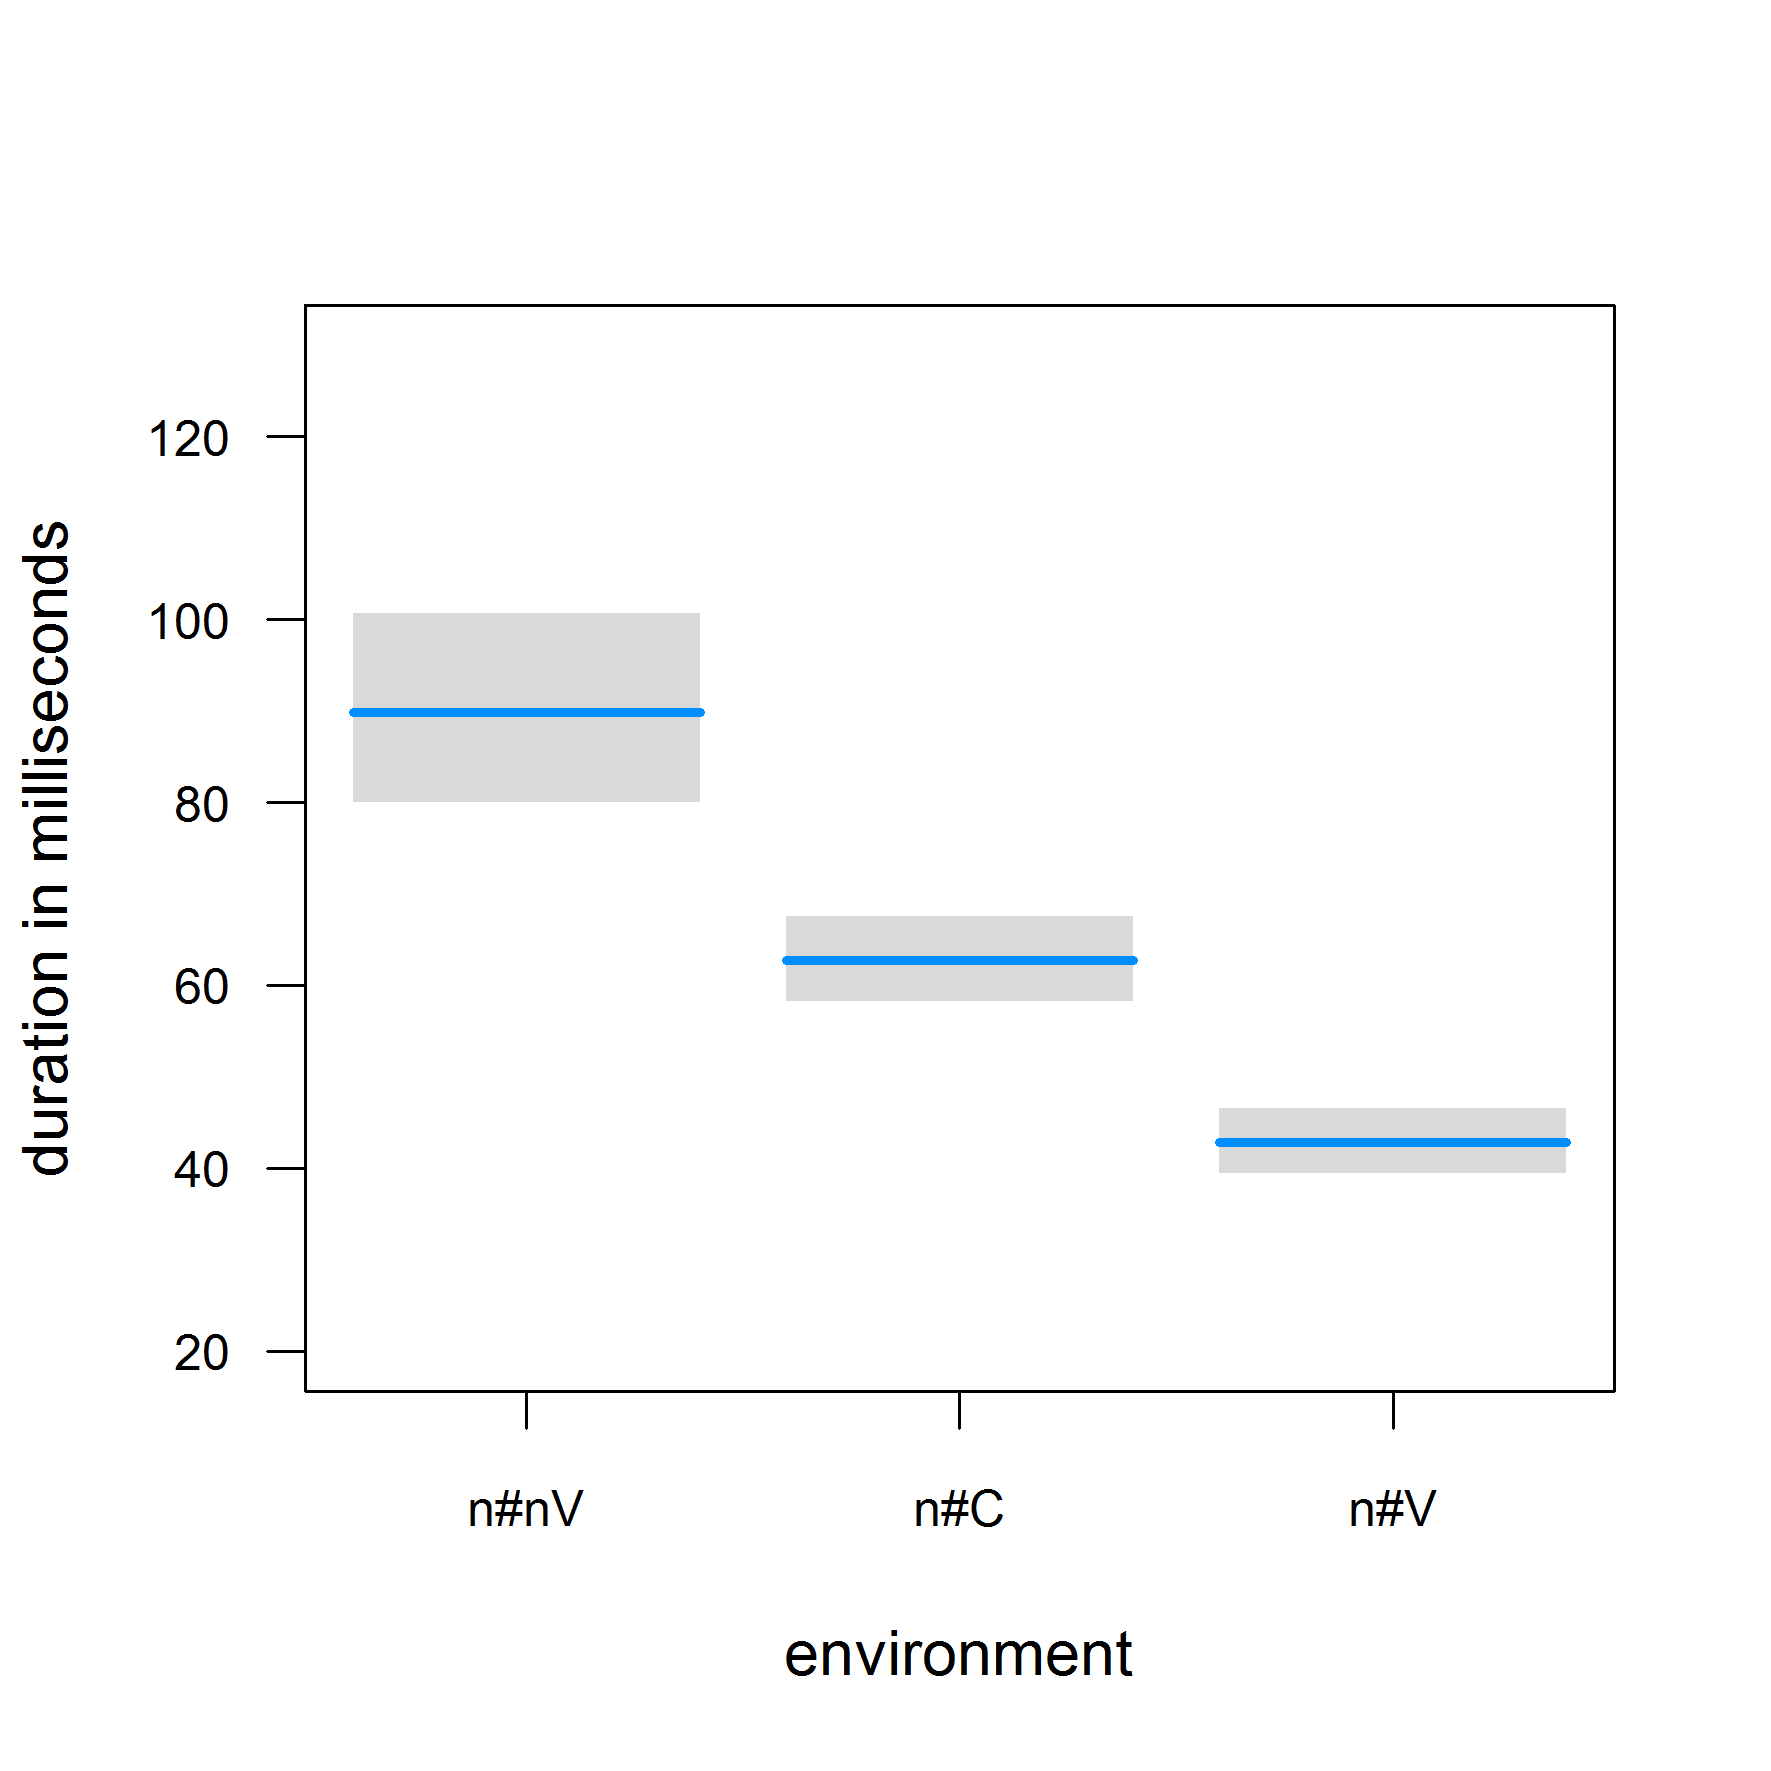
\includegraphics [scale=0.4] {images/Corpus/unModelNumNasal.png}
	\caption{Effect of environment on consonant duration in \prefix{un}data set}
	\label{fig:NumNasal un}
\end{figure}




The predicted mean duration for double nasals is 90~ms. For words with the \texttt{n\#C} environment the nasal is predicted to be 63~ms long, and for words having the \texttt{n\#V} environment it is predicted to be 43~ms long. If we compare the two environments with a following vowel (and thus hold the type of following segment constant), the model predicts double nasals to be even a bit longer than twice the duration of the average single nasal in this environment (90~ms as against 43~ms). This result clearly speaks in favor of \isi{gemination} with \is{un-}\prefix{un}.

When a consonant follows the single nasal at the morpheme boundary, we also find a highly significant contrast between the two environments, but the difference is smaller. We do not find twice the duration for the double nasal, but only a difference of 27 ms, i.e. an increase in duration of 43\% from single to double nasal. 

The question may be raised whether this increase in phonetic duration can be interpreted as \isi{gemination} in spite of the fact that the duration is not doubled. The literature on \isi{gemination} has shown, however, that the durational differences between geminates and their corresponding singletons may vary substantially (see \sectref{what is gemination} for discussion). 
For /n/ in English, differences between 34\% and 109\% were found. For word boundary geminates, \cite{Delattre.} finds  an increase from singleton to geminate /n/ of 50\%.  All investigated environments in \citeauthor{Delattre.}'s study were, however, vowel-initial.  For \isi{normal speech}, \citet[86, Figure 2]{Oh.2012} arrive at an estimated 82~ms for word-internal singletons, 110~ms for \is{un-}\prefix{un}geminates and geminates across word boundaries. This is an increase of 60\%. For \isi{careful speech}, they find estimated durations of 110~ms for singletons, 225~ms for \is{un-}\prefix{un}geminates, and 230~ms for geminates across word boundaries. This is an increase of 104\% to 109\%.\footnote{\citet{Oh.2012} do not give the estimated means in their article. The figures given here are read off from the partial effects plot given in Figure 2 of their article.} Note that again, only vocalic environments were tested.

The comparison to previous findings on \isi{gemination} with English /n/ shows that there is good reason to interpret even the smaller of the two contrasts in the data (i.e. the one between \texttt{n\#C} vs. \texttt{n\#nV}) as evidence for \isi{gemination}. While some studies have found bigger singleton-geminate ratios, some found smaller ratios. Differences in experimental set-up, especially speech condition, and  environment might be the cause of the different ratios found. In this study, the smaller singleton-geminate ratio between pre-consonantal singletons and doubles  (as against the ratio of pre-vocalic singletons and doubles) can be attributed to the type of following segment (C vs. V). As discussed in \sectref{variables of interest}, following consonants generally lead to longer durations for nasals.

After fitting the \is{regression model}{linear model}, \isi{multi-model inferencing} was used to detect which of the variables included in the initial model are the most predictive variables across a multitude of models. The variable \textsc{LSAScore} was not included in the \isi{multi-model inferencing} analysis because of the low number of items which were coded for \textsc{LSAScore}. 
The analysis revealed that the two most important variables are those which also ended up in the final \is{regression model}{linear model}, i.e. \textsc{Environment} (importance value: $1$) and \textsc{LocalSpeechRate} (importance value: $1$).  The importance values of the other variables are much lower (\textsc{PrecedingSegment-Duration}:  $0.4$, \textsc{BaseInitialStress}: $0.29$, log\textsc{WordFormFrequency}: $0.27$, log\textsc{Re-lativeFrequency}: $0.33$). This indicates that these variables are far less predictive of nasal duration than \textsc{Environment} and \textsc{LocalSpeechRate}. 


\subsubsection{Relative duration}


The model predicting relative consonant duration with \is{un-}\prefix{un} was fitted similarly to the model predicting \is{absolute duration}absolute consonant duration and the same interactions were tested. Again the dependent variable was transformed using Box-Cox-transformation to achieve a normal distribution of residuals. The transformation parameter was $0.141$. In contrast to the \isi{absolute duration} model, no outliers had to be excluded. 
 \tabref{tbl: summary corpus un rel dur} summarizes the final model. The model explains about 33\% of the variance and features only one variable, \textsc{Environment}.



\begin{table*}
	\caption{ Summary of linear model for variables predicting the Box-Cox-transformed relative duration of [n] in \prefix{un}prefixed words}
	\label{tbl: summary corpus un rel dur}
	
		
	\resizebox{\textwidth}{!}{%		
		\begin{tabular}{lrrrr}
			
			
			\lsptoprule
			& Estimate & Std. Error & t-value & p-value  \\ 
			\midrule
			
			Intercept       & 1.029  &0.013 & 80.326  &   	$<$ 0.001\\ 
			
			\textsc{Environment}-\texttt{n\#C}  &-0.072 &  0.015  &-4.858 & $<$ 0.001\\ 
			
			\textsc{Environment}-\texttt{n\#V}    &-0.127  & 0.015 &  -8.527 &   $<$ 0.001\\ 
			
			\midrule\\
			Adjusted R-squared:  0.327 \\
			\lspbottomrule
		\end{tabular}
}		
	
\end{table*}



The model reveals that, as in \isi{absolute duration}, double /n/ is significantly longer than both singleton /n/s in \isi{relative duration}. It thus confirms the results of the \isi{absolute duration} model, i.e. \prefix{un} geminates. In contrast to the \isi{absolute duration} model, the variable \textsc{LocalSpeechRate} is not significant in this model. This is not surprising, as the dependent variable \textsc{RelativeConsonantDuration} does not measure duration per se, but the relation of consonant duration and preceding vowel duration, i.e. a ratio. While \isi{speech rate} is known to affect \isi{absolute duration}, an effect on \isi{relative duration} is not expected. 

Multi-model inferencing confirms the final model. The variable \textsc{Environment} is the most predictive variable (importance value: $1$). All other variables have very low importance values  (log\textsc{WordFormFrequency}: $0.56$, \textsc{BaseInitialStress}: $0.46$, \textsc{LocalSpeechRate}: $0.26$, log\textsc{RelativeFrequency}: $0.26$).


\subsubsection{Summary}

Two models were fitted to predict consonant duration with  \is{un-}\prefix{un}. The model predicting \is{absolute duration}absolute consonant duration explains more variance than the one predicting relative consonant duration, i.e. the \isi{absolute duration} model is the better model. In the \isi{absolute duration} model, the noise variable \textsc{LocalSpeechRate} had the expected effect. In the \isi{relative duration} model, no noise variables remained in the final model.
 Both models found a significant effect of the variable \textsc{Environment}. Phonological doubles (\texttt{n\#nV}) are significantly longer than phonological singletons, irrespective of whether the following segment is a consonant (\texttt{n\#C}) or a vowel (\texttt{n\#V}). The durational difference between doubles and singletons is more pronounced when the singleton is followed by a vowel, i.e. a following consonant lengthens the prefixal /n/. The results clearly show that the prefix \is{un-}\prefix{un} geminates.
With regard to the other variables of interest, only \textsc{LSAScore} and log\textsc{RelativeFrequency} could be tested. Neither had a significant effect. 


\subsection{The prefix \prefix{in}} \label{in corpus}


\subsubsection{Absolute duration}

The initial \is{in-}\prefix{in}model predicting \isi{absolute duration} showed a non-normal distribution of residuals. Therefore, the dependent variable was  transformed (Box-Cox-transformation  parameter: $0.465$). After the transformation, the model showed a satisfactory distribution of residuals. The model was then fitted according to the strategy described in \sectref{stats} and interactions were tested (see \hyperref[Appendix C: Summaries of tested interactions in corpus study]{appendix C} for a list of all tested interactions). 
To avoid \isi{collinearity}, the effects of the \is{decomposability measure}decomposability variables were tested individually.


The final model explains about 50\% of the variance in the data and includes four variables with a significant effect on consonant duration, \textsc{Environment}, \textsc{LocalSpeechRate}, \textsc{BaseInitialStress} and \textsc{Affix}. None of the tested interactions proved to be significant. 
An overview of the model coefficients is given in \tabref{tbl: summary model2}.% \pagebreak



\begin{table*}

	\caption{ Summary of linear model for variables predicting the Box-Cox-transformed duration of [m] in \prefix{in}prefixed words}
	\label{tbl: summary model2}
	
	\resizebox{\textwidth}{!}{%		
		\begin{tabular}{p{8cm}rrrr}
			
			
			\lsptoprule
			& Estimate & Std. Error & t-value & p-value  \\ 
			\midrule
			Intercept                              &  0.368 &    0.015 & 24.931 & $<$ 0.001\\
			\textsc{Environment}-\texttt{m\#C}   & -0.048 &    0.007 & -6.662 &  $<$ 0.001\\ 
			\textsc{LocalSpeechRate}  				   &  -0.003&    0.001&  -4.335 & $<$ 0.001\\
			\textsc{BaseInitialStress}-\texttt{unstressed}    & -0.038 &  0.008& -4.826&  $<$ 0.001\\ 
			\textsc{Affix}-\texttt{inNeg}          & 0.016  & 0.007 & 2.121 &   0.036\\ 
			\midrule\\
			Adjusted R-squared: $0.504$\\
			\lspbottomrule
		\end{tabular}
 }	
	

\end{table*}


\figref{fig:covariates in} displays the effects of the two noise variables in the model. The left panel shows the effect of  \textsc{LocalSpeechRate}. This effect is as expected: 
the higher the \isi{speech rate}, the shorter the nasal. The right panel shows the effect of \textsc{BaseInitialStress}. With an estimated mean duration of 74~ms, the consonant is 21~ms shorter before an unstressed base-initial syllable than before a \is{stress}stressed base-initial syllable (95~ms). This result is expected, too. As mentioned in \sectref{General method annotation}, \cite{Umeda.1977} also found that nasals before unstressed vowels are shorter than nasals before \is{stress}stressed vowels.

\begin{figure*}
	
	
	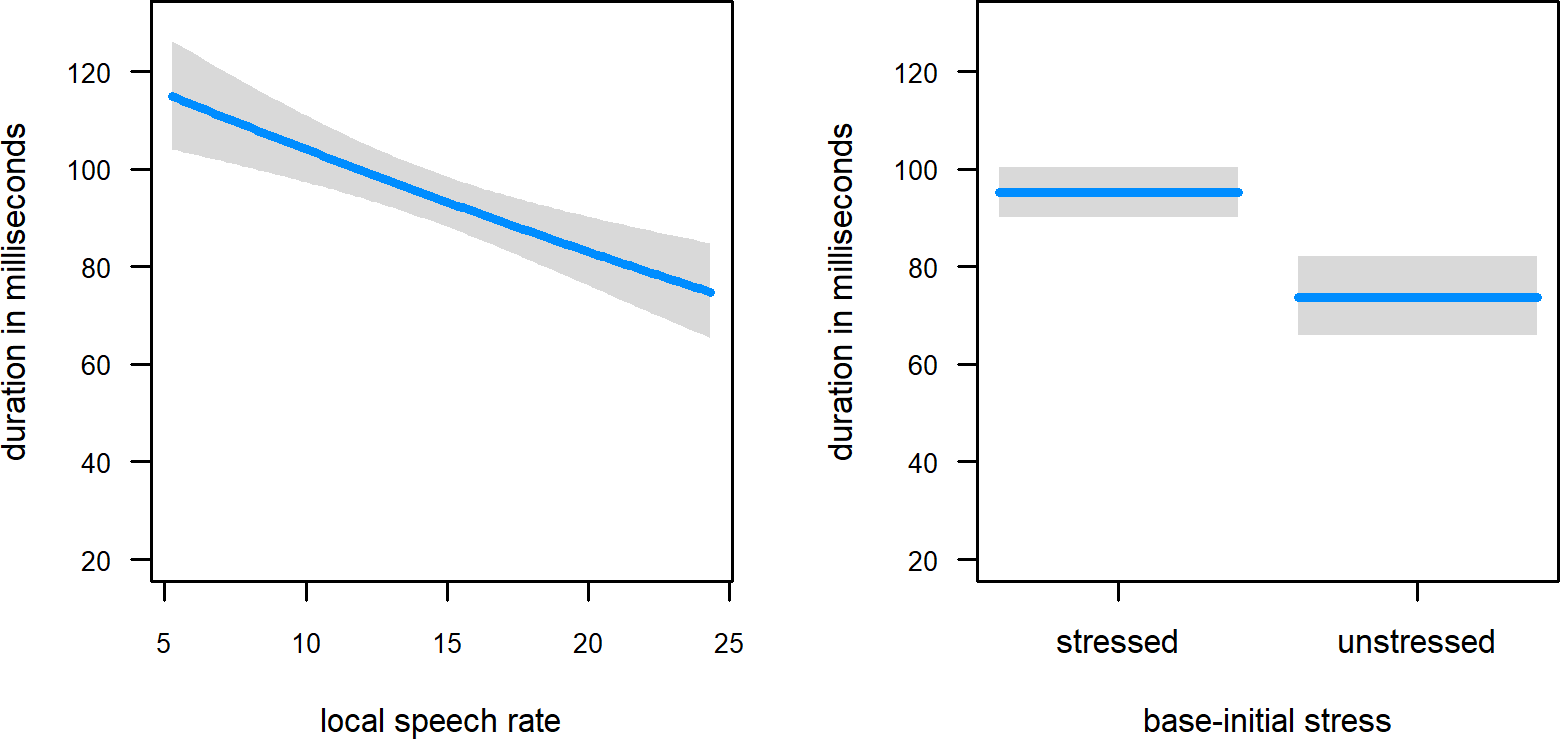
\includegraphics  [scale=0.8] {images/Corpus/inModelcov.png}
	\caption{Effects of local speech rate and base initial-stress on consonant duration in \prefix{in}data set}
	\label{fig:covariates in}
\end{figure*}

Let us turn to the variables of interest. The left panel of \figref{fig:inModel} displays the effect of \textsc{Environment}. Double consonants are significantly longer than singletons. The estimated mean duration for double consonants is 95~ms, while it is 68~ms for single consonants, a difference of 27~ms. This difference is significant, and shows that \is{in-}\prefix{in} geminates. 







\begin{figure*}
	
	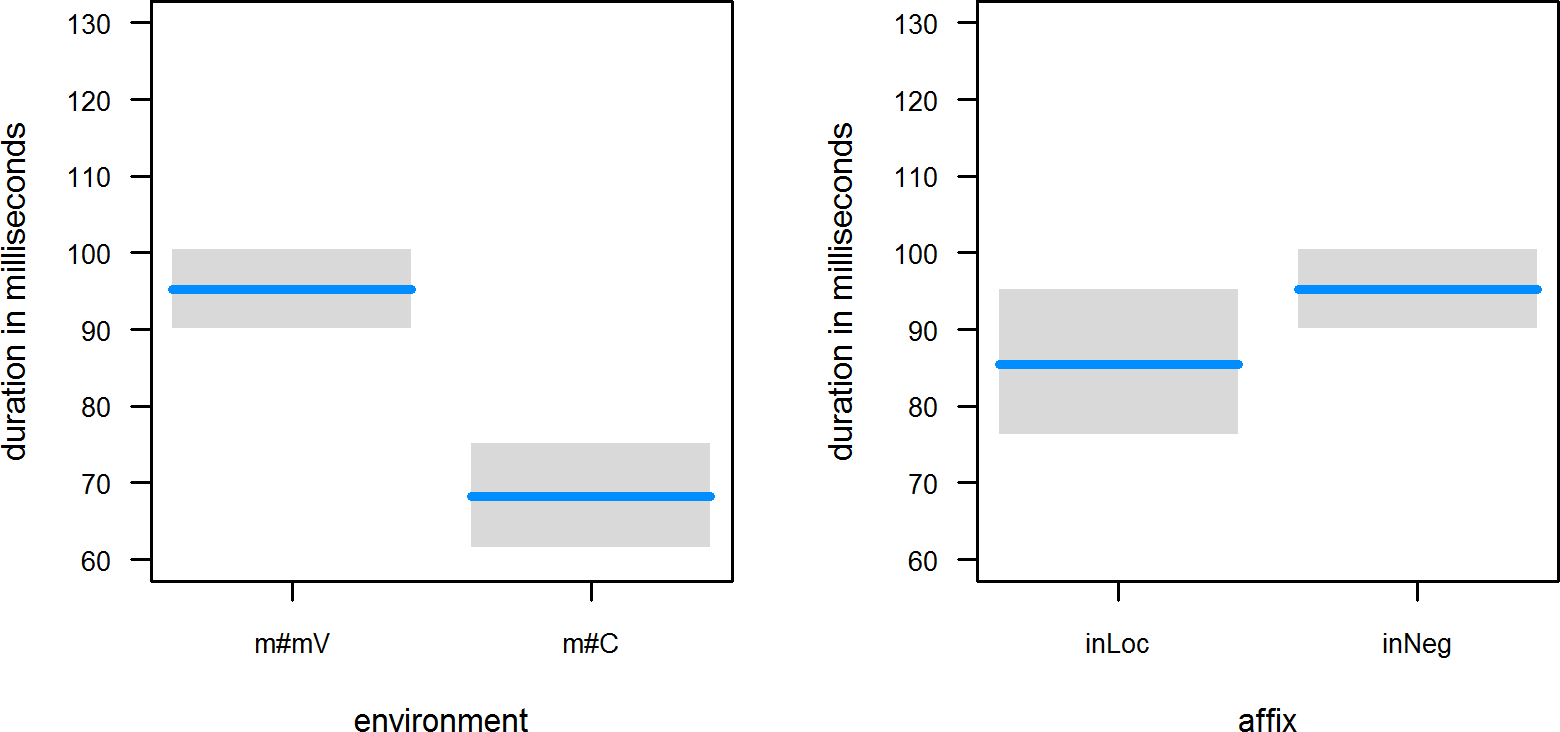
\includegraphics [scale=0.8]  {images/Corpus/inModel.png}
	\caption{Effects of environment and affix on consonant duration in \prefix{in}data set}
	\label{fig:inModel}
\end{figure*}



However, one could venture the idea that the difference is not due to a difference between one consonant and two, but due to a difference in the following segment, i.e. consonant versus vowel. This idea is, however, unsupported, since following vowels lead to shorter durations of the nasal. This can also be seen in the \is{un-}\prefix{un}data set, in which a single nasal preceding a consonant (63~ms) is longer than a single nasal preceding a vowel (43~ms). In other words, the double nasals (which are by their very nature followed by a vowel) are likely to be shortened, not lengthened, due to their vocalic environment. In other words, the double nasals show longer duration in spite of being in an environment that would trigger shorter duration. The significant difference between \texttt{m\#mV}  and \texttt{m\#C} is thus a sure sign of \isi{gemination}.



The effect of \textsc{Affix} is displayed  in the right panel of \figref{fig:inModel}. The nasal in \is{negative in-}negative \prefix{in} is significantly longer (by 10~ms) than the one in \is{locative in-}locative \prefix{in}. Hence, there is a difference in the duration of the nasal depending on which of the two affixes is used. There was no interaction of \textsc{Environment} and \textsc{Affix}, which means that the two prefixes do not differ significantly in their \isi{gemination} behavior.


None of the investigated \is{decomposability measure}decomposability measures proved to be significant. However, it is possible that, while the measures do not affect duration when tested individually, a combined measure of \isi{decomposability} has a significant effect on consonant duration. As evidenced by the \isi{decomposability} analyses in \sectref{corpus dec}, at least some of the \is{decomposability measure}decomposability variables highly correlate and can be assumed to measure the same underlying property. It is thus possible to test the effect of a combined measure of this underlying property. 

To test the effect of a combined \isi{decomposability} measure, an additional model with combined \is{decomposability measure}decomposability measures (as opposed to individual \is{decomposability measure}decomposability measures) was fitted. The combined measures were created by means of a \is{principal component analysis}principal component analysis (cf. \sectref{stats} on \is{principal component analysis}principal component analyses). 
The \is{principal component analysis}principal component analysis was fitted with the variables log\textsc{Relative-Frequency}, \textsc{SemanticTransparency}, \textsc{SemanticTransparencyRating}, \textsc{TypeOfBase} and \textsc{Affix}. The variable \textsc{Affix} was included because of the differences in \isi{segmentability} between locative and \is{negative in-}negative \prefix{in} (see \sectref{The decomposability of the four affixes: a comparison} for discussion). \textsc{LSAScore} was excluded because of the low number of observations coded for this variable. Categorical variables were recoded as numerical before entering the analysis, and all variables were scaled.
\tabref{tbl: summary PC in corpus} summarizes the analysis by showing the composition of each \is{principal component analysis}principal component, i.e. the loading of each variable for each \is{principal component analysis}principal component, and by displaying the proportion of variance covered by each component. 


\begin{table}
	\caption{ Summary of principal components}
	\label{tbl: summary PC in corpus}
	
			\resizebox{\textwidth}{!}{%		
		\begin{tabular}{lrrrrr}
			
			
			\lsptoprule
			
			
			\multicolumn{6}{l}{\textbf{Composition of principal components}}\\
			
			&PC1&          PC2 &       PC3       & PC4 & PC5  \\
			\midrule
			scaled\textsc{Affix }   &   0.078& -0.817 &-0.244 &0.449 & 0.255\\
			scaled\textsc{RelativeFrequency } &  -0.428& 0.450&-0.530 &0.574 & 0.054\\ 
			scaled\textsc{SemanticTransparencyRating}  &   -0.521&-0.233&  0.450& 0.269& -0.631\\
			scaled\textsc{TypeOfBase }&-0.487&-0.275 &-0.529&-0.623& -0.140\\
			scaled\textsc{SemanticTransparency }& -0.550& -0.002 & 0.420&-0.087&  0.717\\
			
			
			\midrule
			\multicolumn{6}{l}{\textbf{Variance explained by principal components}}\\
			&PC1&          PC2 &       PC3       & PC4 & PC5  \\
			\midrule
			Proportion of Variance &0.551& 0.264&  0.086& 0.064 &0.035\\
			\lspbottomrule                                                                                
		\end{tabular}
}
	


\end{table}



The analysis revealed that the first two components can account for most of the variance expressed by the five variables (81\%). An inspection of the rotation matrix shows that the first component is dominated by all four \is{decomposability measure}decomposability measures, and that the second is mainly dominated by the variable \textsc{Affix}. One can thus conclude that the first component represents a combined measure of \isi{decomposability}, and the second represents the variable \textsc{Affix}. 
Both components were included as predictor variables in the \is{regression model}{linear model}.  



The \is{regression model}{linear model} with the principal components was fitted similarly to the model with the individual \is{decomposability measure}decomposability measures. After simplification, the model showed very similar effects as the model with the individual \is{decomposability measure}decomposability measures (see \hyperref[Appendix D: model summaries corpus]{appendix D} for model summary). The effects of \textsc{Environment}, \textsc{LocalSpeechRate} and \textsc{BaseInitialStress} are identical. Instead of the variable \textsc{Affix}, this model shows an effect of \textsc{PC2}. The effect is shown in \figref{fig:PC2 in Corpus}. The higher the value of \textsc{PC2}, the longer the duration of the nasal. As explained above, \textsc{PC2} is dominated by the variable \textsc{Affix}. A higher \textsc{PC2}-value indicates \is{negative in-}negative \prefix{in}, a lower \textsc{PC2}-value indicates \is{locative in-}locative \prefix{in}. One can thus interpret the effect of \textsc{PC2} as being an effect of \textsc{Affix}. Negative \prefix{in} is longer than \is{locative in-}locative \prefix{in}. The principal component model hence shows the same effects as the model with the individual \is{decomposability measure}decomposability measures.


\begin{figure*}
	
	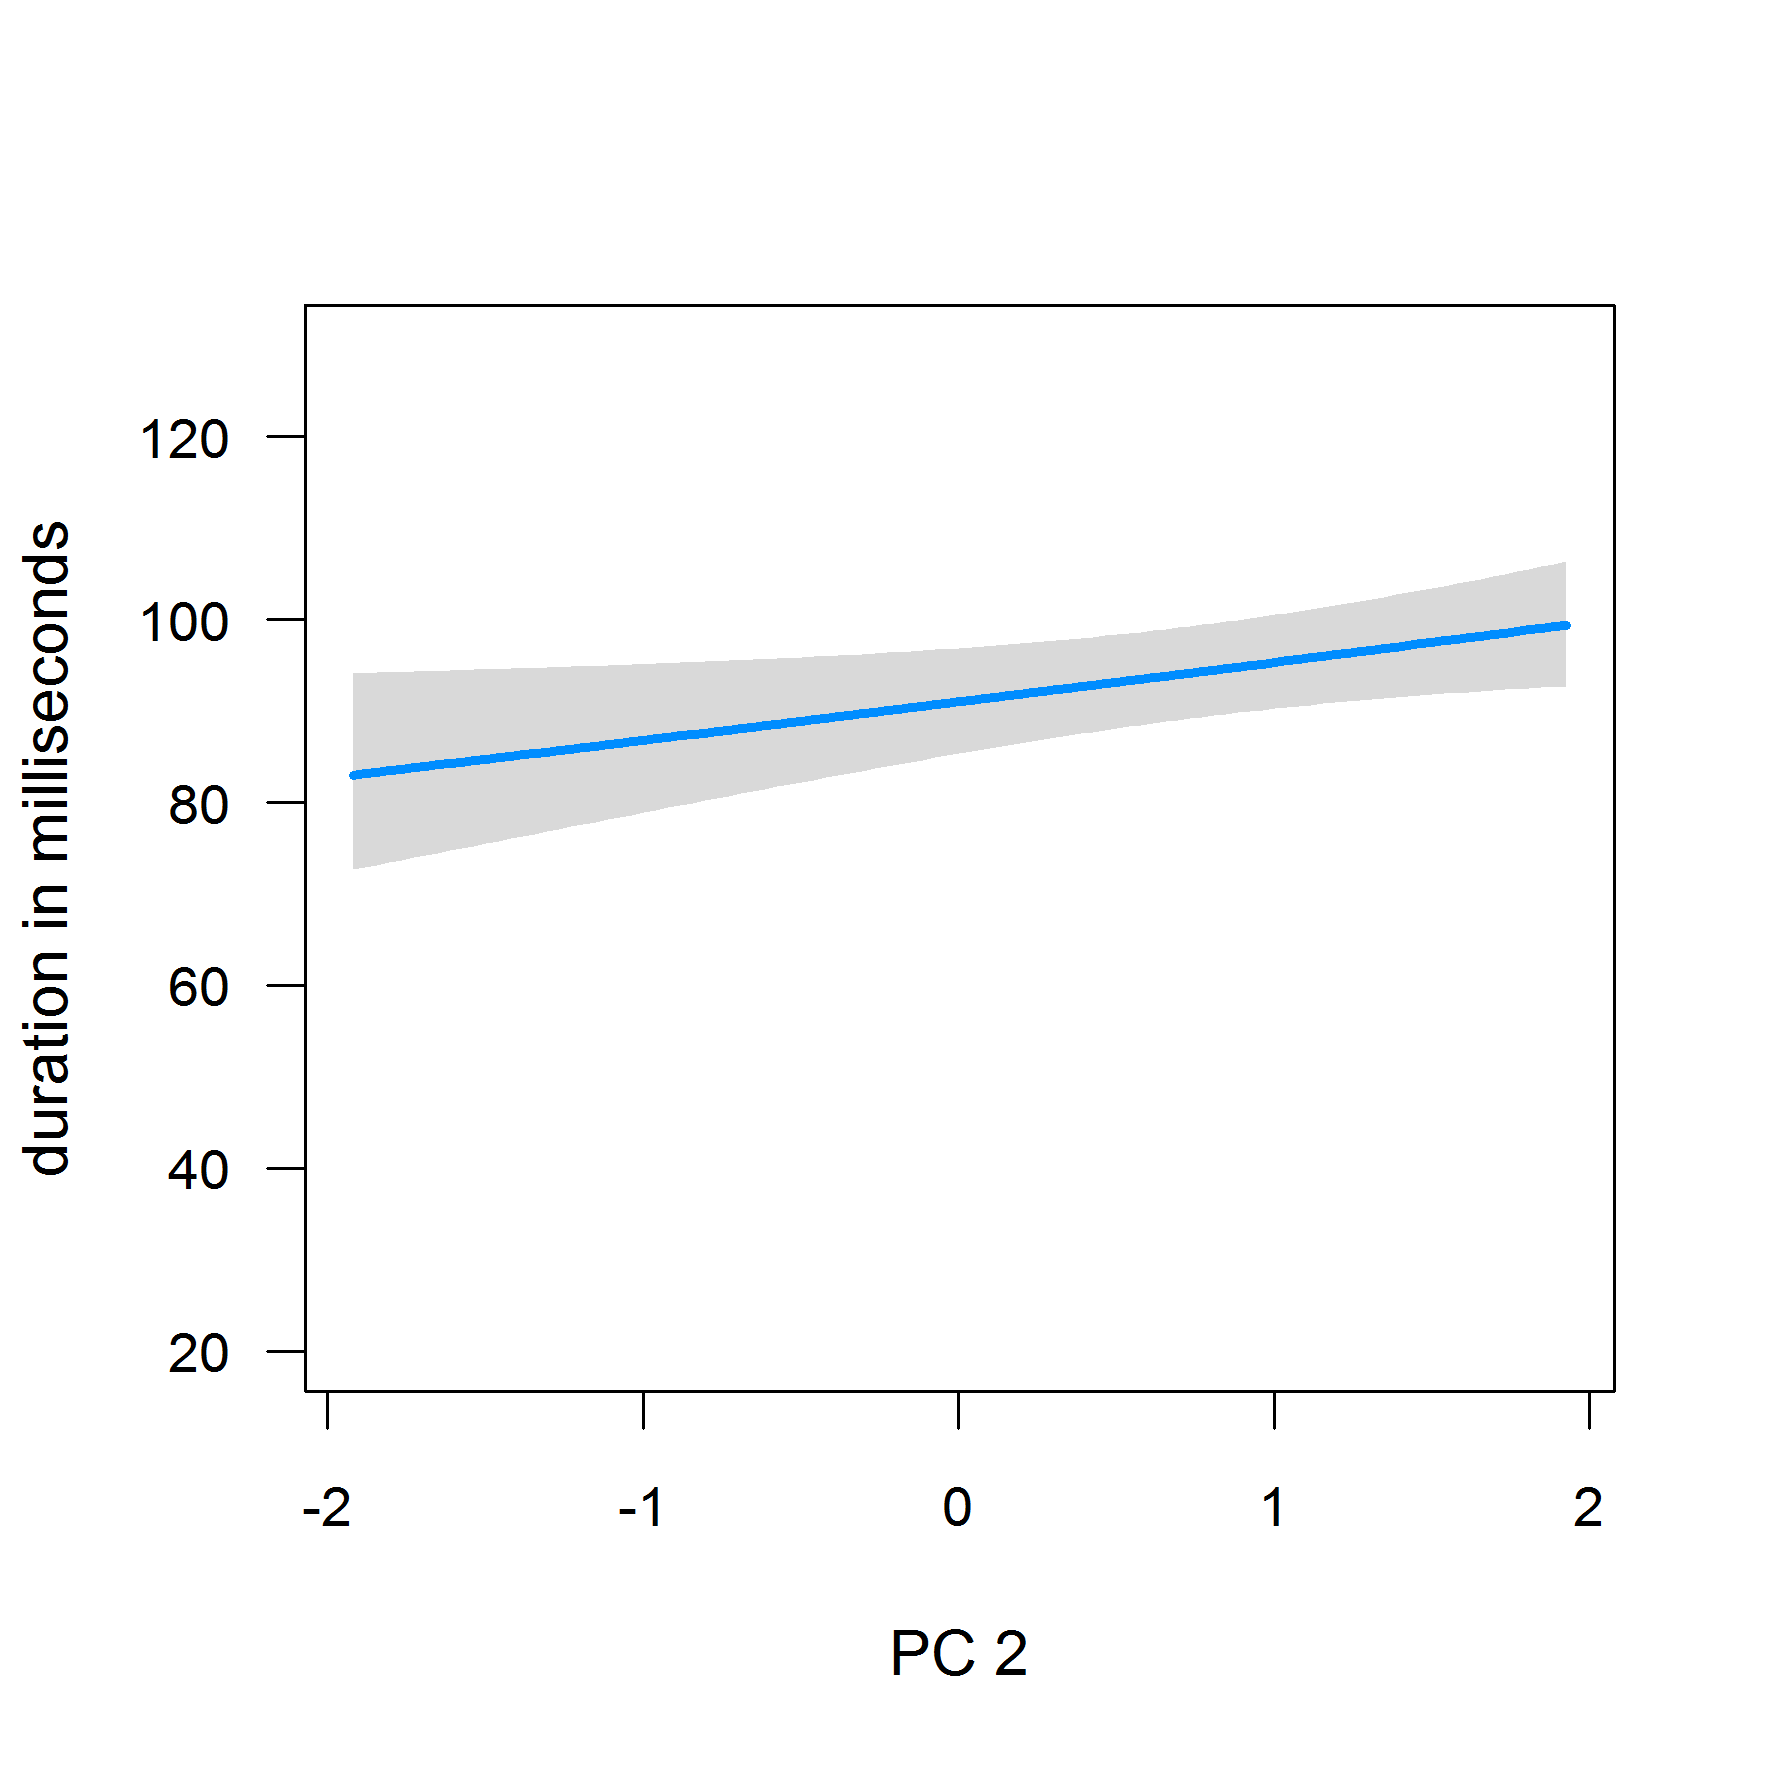
\includegraphics [scale=0.4] {images/Corpus/imPCAbsPC2.png}
	\caption{Effect of PC2 on consonant duration in \prefix{in}data set}
	\label{fig:PC2 in Corpus}
\end{figure*}



After the final models were fitted, \isi{multi-model inferencing}  was used to detect the most important predictor variables. Due to the \isi{collinearity} problems with the \is{decomposability measure}decomposability variables, these variables were not included separately in the analysis. Instead, the combined \isi{decomposability} measure from the \is{principal component analysis}principal component analysis, i.e. \is{principal component analysis}principal component 1 (\textsc{PC1}), was included.
The analysis revealed that \textsc{LocalSpeechRate}, \textsc{Environment} and \textsc{BaseInitialStress} are the most predictive variables. They all have an importance value of $1$. \textsc{Affix} has an importance value of $0.79$, i.e. it is the fourth most important variable. With importance values of $0.29$ (\textsc{PC1}), $0.28$ (log\textsc{WordFormFrequency}) and $0.27$ (\textsc{PrecedingSegmentDuration}), the other variables are far less predictive of consonant duration. Multi-model-inferencing thus confirms the results of the final models.


\subsubsection{Relative duration}

In the model predicting relative consonant duration with \is{in-}\prefix{in}, the dependent variable was Box-Cox-transformed by the parameter $-0.101$ to achieve a normal distribution of the residuals. No outliers were excluded. The model was fitted similarly to the \isi{absolute duration} model, i.e. the same interactions were tested and the \is{decomposability measure}decomposability measures were tested in the same way. On the one hand the \is{decomposability measure}decomposability variables were tested individually. On the other, \isi{decomposability} was tested by means of principal components in an additional model. 

The simplification of both models, i.e. the one with the individual measures and the one with the principal components, resulted in same final model. The model features the three predictor variables \textsc{Environment}, \textsc{LocalSpeechRate} and \textsc{BaseInitialStress}. Neither the individual \is{decomposability measure}decomposability measures nor the principal components proved to be significant. There are no interactions. 
The summary of the final model is given in \tabref{tbl: summary model rel du in corpus}. The model explains about 42\% of the variance in the data.\\





\begin{table*}
	\caption{ Summary of linear model for variables predicting the Box-Cox-transformed relative duration of [m]  in \prefix{in}prefixed words}
	\label{tbl: summary model rel du in corpus}
	
			\resizebox{\textwidth}{!}{%		
		
		\begin{tabular}{lrrrr}
			
			
			\lsptoprule
			& Estimate & Std. Error & t-value & p-value  \\ 
			\midrule
			
			Intercept       & 0.987 & 0.015 & 65.285  &   	$< $0.001\\ 
			
			\textsc{Environment}-\texttt{m\#C } & 0.053 &   0.007 & 7.308 &$< $0.001\\ 
			
			
			\textsc{LocalSpeechRate}  				  &  -0.003 & 0.001 &  -3.416 & 0.001 \\ 
			
			\textsc{BaseInitialStress}-\texttt{unstressed}    & 0.066 &  0.008 & 7.876 & $< $0.001\\ 
			
			\midrule\\
			Adjusted R-squared: 0.422 \\
			\lspbottomrule
		\end{tabular}
}
	


\end{table*}


As in the model predicting \isi{absolute duration}, this model reveals that double consonants are longer than singletons, i.e. we also find \isi{gemination} in \isi{relative duration}. Also similar to the \isi{absolute duration} model, \textsc{LocalSpeechRate} affects consonant duration. The higher the \isi{speech rate}, the shorter the nasal relative to the vowel. This effect of \isi{speech rate} indicates that \isi{speech rate} has a bigger effect on the consonant of the prefix \is{in-}\prefix{in} than on its vowel, i.e. in faster speech the consonant is more reduced than the vowel. A possible explanation might be that the prefixal vowel in \is{in-}\prefix{in} is too short to be reduced to the same degree as the prefixal nasal, i.e. there is simply less material to be reduced.

The model also reveals a significant effect of \textsc{BaseInitialStress}. In \isi{relative duration}, the consonant is longer before unstressed syllables. This is the opposite of what is found for \isi{absolute duration}, where the consonant is shorter in that condition. 
This difference between relative and \isi{absolute duration} can be explained by the role of the preceding vowel for \isi{relative duration}. Longer preceding vowels lead to shorter relative durations. One can thus assume that the shorter \isi{relative duration} of the consonant in words with an unstressed base-initial syllable is caused by a longer preceding vowel in those words.
Longer vowels before unstressed syllables are expected. This is because, in the investigated words, unstressed base-initial syllables indicate a \is{stress}stressed prefix, which in turn might influence the duration of the prefixal vowel. It is particularly the duration of the vowel which is lengthened in a \is{stress}stressed syllable, i.e. one might expect the vowel of a \is{stress}stressed prefix (which is followed by an unstressed syllable) to be lengthened. A longer vowel in turn leads to shorter \isi{relative duration}. This explains that in \isi{relative duration} the consonant is shorter before unstressed base-initial syllables than before \is{stress}stressed base-initial syllables.
The \isi{absolute duration} of the consonant, in contrast to its \isi{relative duration}, is not affected by the duration of the preceding segment, i.e. by its \isi{stress} status. Instead, the consonant participates in the stress-caused lengthening of its following syllable, i.e. the consonant is longer before \is{stress}stressed base-initial syllables. %The reverse effect of \textsc{BaseInitialStress} can thus be explained by the role of preceding vowel duration.

In contrast to the absolute model, in the \isi{relative duration} model \textsc{Affix} does not have a significant effect. This indicates that negative and \is{locative in-}locative \prefix{in} only differ in \isi{absolute duration}, i.e. the ratio of consonant and vowel duration does not differ between the two prefixes. 
As with \isi{absolute duration}, no effect of the \is{decomposability measure}decomposability variables was found in the \isi{relative duration} models. 

Multi-model inferencing revealed that the three variables which are significant in the final model are the most predictive variables across a multitude of models. \textsc{BaseInitialStress} has an importance value of $1$, \textsc{Environment}  has an importance value of $0.99$,  and  \textsc{LocalSpeechRate} has an importance value of $0.99$. The other tested variables are much less predictive of \isi{relative duration} (importance value of log\textsc{WordFormFrequency}: $0.54$, importance value of \textsc{Affix}: $0.48$, importance value of \textsc{PC1}: $0.37$). 


\subsubsection{Summary}


The two linear models predicting consonant duration with \is{in-}\prefix{in} clearly show that locative and \is{negative in-}negative \prefix{in} geminate. In both models, phonological doubles are longer than phonological singletons. 
The \isi{absolute duration} model furthermore revealed that the nasal in \is{negative in-}negative \prefix{in} is significantly longer than the one in \is{locative in-}locative \prefix{in}, irrespective of whether it is a double consonant or a singleton. This effect of \textsc{Affix} was, however, not found in \isi{relative duration}.
With regard to the \isi{decomposability} measure, none had an effect on nasal duration, neither in absolute, nor in \isi{relative duration}. 
In both models, the two noise variables \textsc{LocalSpeechRate} and \textsc{BaseInitialStress} showed expected effects. None of the tested interactions was significant. 
The model predicting \is{absolute duration}absolute consonant duration explains more of the variance in the data than the model predicting \isi{relative duration}. 



\subsection{The prefixes \prefix{un} and \prefix{in}} \label{corpus un in}


The model predicting consonant duration with \is{un-}\prefix{un} and \is{in-}\prefix{in} was fitted to directly compare the durational behavior of the nasals in the three prefixes \is{un-}\prefix{un}, \is{negative in-}negative \prefix{in} and \is{locative in-}locative \prefix{in}. The model has, however, the disadvantage that a number of interesting variables cannot be properly tested. The reason is that the \is{un-}\prefix{un} data set and the \is{in-}\prefix{in}data set differ in important respects.
First, the prefix \is{un-}\prefix{un} and the allomorph of \is{in-}\prefix{in} that is being invested here end in two different consonants, i.e.  /n/ vs. /m/. Therefore, durational differences between \is{un-}\prefix{un} and \is{in-}\prefix{in} are not directly comparable. I  used scaling of the durational variables to alleviate this problem. This, however, means that durational differences are not straightforward in their interpretation. 
Second, the phonological environments of singleton \is{un-}\prefix{un} and singleton \is{in-}\prefix{in} are not the same, since \is{im-}/ɪm/ is necessarily always followed by a base-initial consonant, while \is{un-}\prefix{un} is followed by both consonants and vowels. Only the double nasal in both prefixes is always followed by a vowel.
Third, variables of \isi{decomposability}  cannot be tested in an interesting way. This is because \is{un-}\prefix{un}, as described in \sectref{The decomposability of the four affixes: a comparison}, does not vary in most of the \is{decomposability measure}decomposability measures, and because \isi{relative frequency} measures are not well comparable across \is{un-}\prefix{un} and \is{in-}\prefix{in}. The prefix \is{in-}\prefix{in} has very many bound roots, which is problematic with regard to computing \isi{relative frequency} measures that are comparable to the \isi{relative frequency} measures of affixes with hardly any or no bound roots, i.e. in this case \is{un-}\prefix{un}. 
With these limitations in mind, a regression model was fitted to the lumped data set.  

Since the environments for the prefixal nasal are not the same across prefixes, I created a new variable in which I coded whether the word has one or two underlying nasals (\textsc{NumberOfConsonants}), and an additional variable encoding whether a vowel or a consonant followed the nasal (\textsc{FollowingSegment}). I included the following predictors in the model: \textsc{NumberOfConsonants}, \textsc{FollowingSegment}, \textsc{LocalSpeechRate},  \textsc{BaseInitialStress}, \textsc{Affix}, \textsc{PrecedingSegmentDuration} and log\textsc{WordFormFrequency}.
The model was then simplified and interactions were tested. Crucially, all interactions between the variable \textsc{Affix} and all other variables were tested (see \hyperref[Appendix C: Summaries of tested interactions in corpus study]{appendix C} for a list of all tested interactions). 
The final model explains 49\% of the variance and features five variables, \textsc{Number-OfConsonants}, \textsc{FollowingSegment}, \textsc{LocalSpeechRate}, \textsc{BaseInitialStress} and \textsc{Affix}. The model is documented in \tabref{tbl:corpus summary model un, in}.




\begin{table*}
	\caption{ Summary of linear model for variables predicting the normalized duration of the nasal in
		\prefix{un} and \prefix{in}prefixed words}
	\label{tbl:corpus summary model un, in}
	
		
			\resizebox{\textwidth}{!}{%				
		\begin{tabular}{lrrrr}
			
			
			\lsptoprule
			& Estimate & Std. Error & t-value & p-value  \\ 
			\midrule
			
			Intercept       & 2.484 &0.223  & 11.127  &   $<$ 0.001\\ 
			
			\textsc{NumberOfConsonants}-\texttt{double } & -1.454  &  0.144 & -10.065 & $<$ 0.001\\ 
			
			\textsc{FollowingSegment}-\texttt{vowel} & -0.537  & 0.130  & -4.136 & $<$ 0.001 \\ 			
			\textsc{LocalSpeechRate}  				  & -0.088 & 0.012 & -7.016 & $<$ 0.001\\ 
			
			\textsc{BaseInitialStress}-\texttt{unstressed}    & -0.347 &  0.103 & -3.365 & 0.001 \\ 
			
			\textsc{Affix}-\texttt{inLoc}   & -0.469  & 0.133 & -3.521 &   0.001\\ 
			\textsc{Affix}-\texttt{un}   & 0.343   & 0.123 & 2.794 &   0.006\\ 			
			\midrule\\
			Adjusted R-squared: 0.49  \\
			\lspbottomrule
		\end{tabular}
}
	
\end{table*}



\begin{figure*}
	
	
	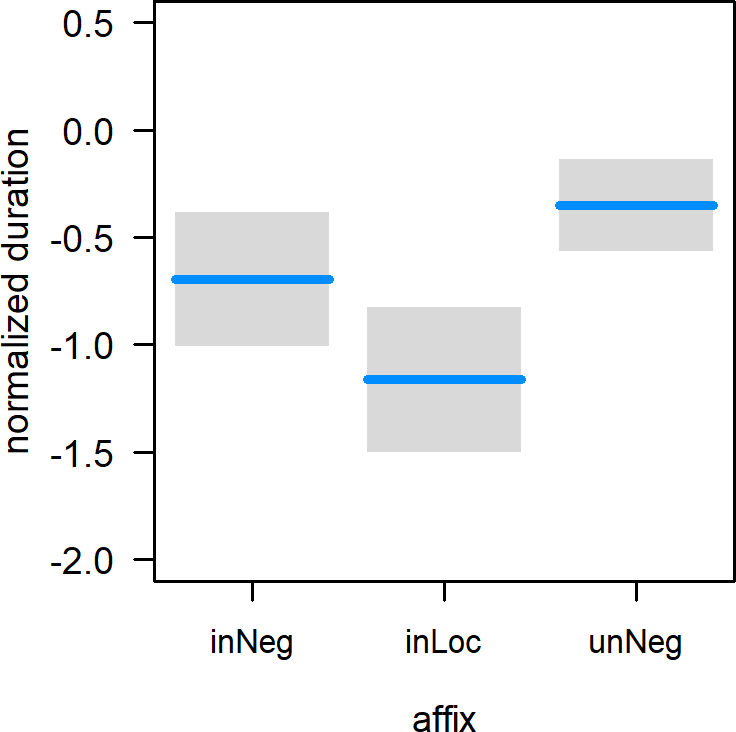
\includegraphics[scale=0.8] {images/Corpus/unInModel.png}
	\caption{Effects of  affix on consonant duration for words prefixed with \prefix{un} and \prefix{in}}
	\label{fig:inUnModel}
\end{figure*}



As in the \is{un-}\prefix{un} and \is{in-}\prefix{in}models, this model shows that doubles are longer than singletons. Interestingly, there is also  a  main effect of \textsc{Affix}. \figref{fig:inUnModel} shows that \is{negative in-}negative \prefix{in} is significantly longer than \is{locative in-}locative \prefix{in}, and that \is{un-}\prefix{un} is significantly longer than \is{negative in-}negative \prefix{in}.  We thus find a decline in duration from \is{un-}\prefix{un}, to \is{negative in-}negative \prefix{in}, to \is{locative in-}locative \prefix{in}. This decline is fully in line with the decline in \isi{segmentability} of the prefixes found in \sectref{The decomposability of the four affixes: a comparison}. Crucially, there is no significant interaction between \textsc{Affix} and \textsc{NumberOfConsonants}, which means that all three prefixes geminate.

In addition to the effects of the variables of interest, there is the expected effect of \textsc{LocalSpeechRate} (nasals become shorter with increasing \isi{speech rate}) and the expected effect of the \textsc{FollowingSegment} (nasals are shorter before vowels). There is also an effect of \textsc{BaseInitialStress} such that the nasal is shorter before unstressed syllables.

\subsection{The prefix \prefix{dis}} \label{corpus results dis}


\subsubsection{Absolute duration}

The residuals of the initial model predicting \is{absolute duration}absolute consonant duration with \is{dis-}\prefix{dis} were not distributed normally. Therefore, the dependent variable was Box-Cox-transformed (parameter:  $0.222$). After the model was refitted with the transformed dependent variable, it showed a satisfactory distribution of residuals. No outliers were removed. The model was then simplified according to the strategy described in \sectref{General Method}  and interactions were tested (see \hyperref[Appendix C: Summaries of tested interactions in corpus study]{appendix C} for a list of all tested interactions).

As in the \is{in-}\prefix{in}model, testing the effect of the \is{decomposability measure}decomposability measures simultaneously was not possible due to \isi{collinearity} problems. Therefore, their effect was tested individually, as well as by using principal components. In other words, first models were fitted in which the effects of the \is{decomposability measure}decomposability measures were tested individually, and then an additional model with a combined \isi{decomposability} measure was fitted. 
 Let us first discuss the model which initially included the individual measures.

An overview of the final model, i.e. the model after simplification, is given in \tabref{tbl: summary model4}. Insignificant estimates are printed in light gray. The model yields an adjusted R-squared of  0.333, i.e. it explains about 33\% of the variance found in the data. The model includes four variables, \textsc{Environment}, \textsc{LocalSpeechRate}, \textsc{Voicing} and \textsc{BaseInitialStress}. There is a significant interaction between \textsc{Environment} and \textsc{BaseInitialStress}. None of the \is{decomposability measure}decomposability variables is significant.


\begin{table*}
	\caption{ Summary of linear model for variables predicting the Box-Cox-transformed duration of [s] in \prefix{dis}prefixed words}
	\label{tbl: summary model4}
	
					\resizebox{\textwidth}{!}{%		
		\begin{tabular}{lrrrr}
			
			
			\lsptoprule
		 	                                     & Estimate & Std. Error & t-value & p-value  \\ 
			\midrule
			 Intercept                             & 0.644 &    0.015 & 43.659& $<$ 0.001\\	
					
			 \textsc{Environment}-\texttt{s\#C}  & -0.045 &    0.009 &  -5.176 & $<$ 0.001\\ 
			
			\textsc{Environment}-\texttt{s\#V}   & -0.026 &   0.010 & -2.506 & 0.014 \\ 
			
			\textsc{LocalSpeechRate}  				  &-0.005 & 0.001 & -4.595  &$<$ 0.001\\ 
			\textsc{Voicing}-\texttt{voiceless}   & 0.057 & 0.011 & 5.367 & $<$ 0.001\\ 		
			
			
			\textsc{BaseInitialStress}-\texttt{unstressed}   & -0.036 &  0.019 & -1.851 & 0.066 \\ 
			

			\textsc{Environment}-\texttt{s\#C}: &&&&\\
			\textsc{BaseInitialStress}-\texttt{unstressed}  & 0.048  &  0.023  & 2.068  & 0.041\\ 
			
			\textsc{Environment}-\texttt{s\#V}: &&&&\\
			\textsc{BaseInitialStress}-\texttt{unstressed}  & \color{lsLightGray}{0.017} & \color{lsLightGray} 0.021 &\color{lsLightGray}0.782  &\color{lsLightGray} 0.436 \\ 
			\midrule\\
			Adjusted R-squared: 0.333 \\
			\lspbottomrule
		\end{tabular}
}
	
\end{table*}






\begin{figure*}
	
	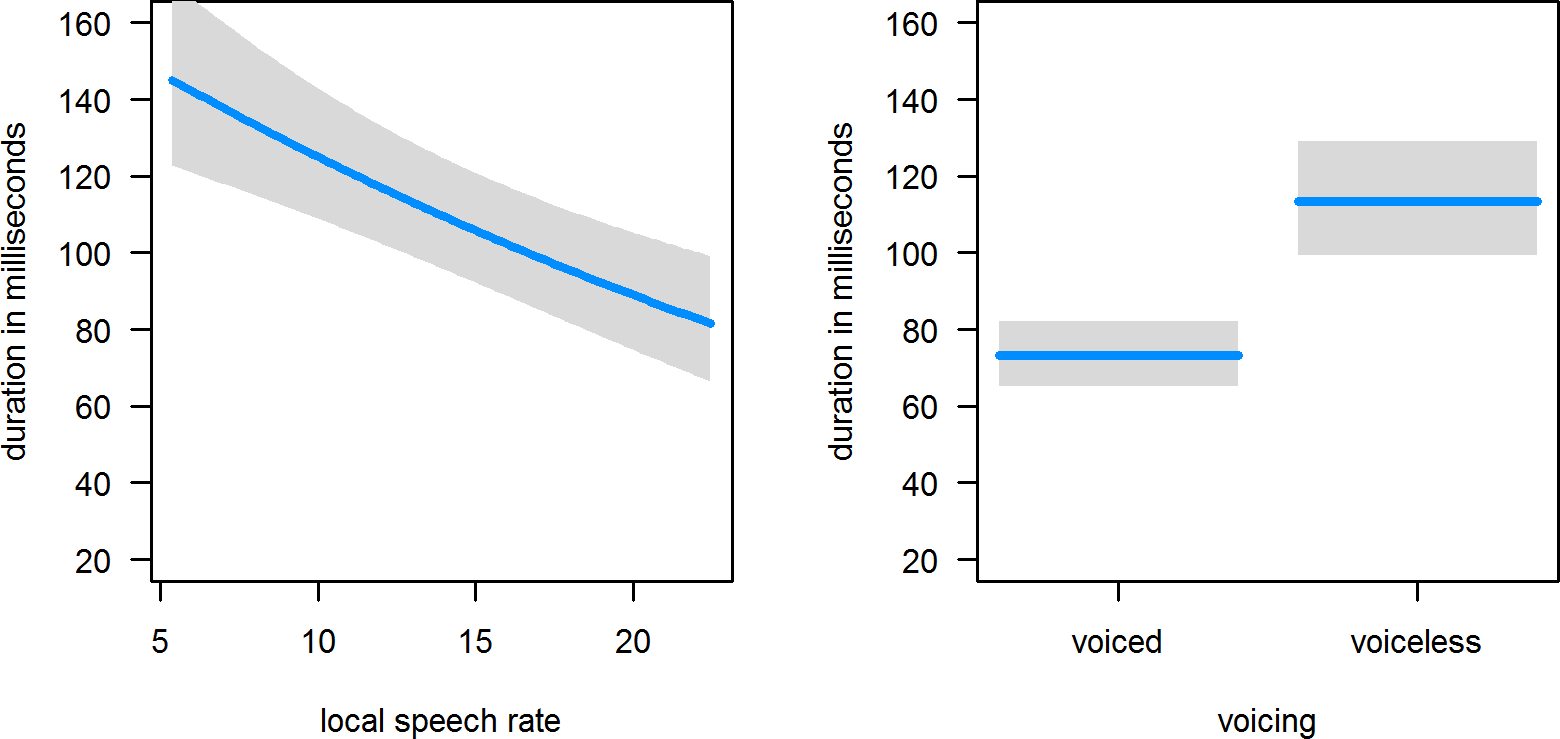
\includegraphics[scale=.8] {images/Corpus/disModelcov.png}
	\caption{ Effect of local speech rate and voicing on consonant duration in \prefix{dis}data set}
	\label{fig:corpus covariates dis}
\end{figure*}


%\isi{speech rate}
\figref{fig:corpus covariates dis} displays the effects of \textsc{LocalSpeechRate} and \textsc{Voicing}. The effect of \textsc{LocalSpeechRate} can be seen in the left panel. As expected, with increasing \isi{speech rate} the fricative in \is{dis-}\prefix{dis}prefixed words becomes shorter. 
%voicing
The right panel of the figure shows the effect of \textsc{Voicing}. Voiced fricatives are significantly shorter than voiceless fricatives. For doubles this difference is predicted to be 47~ms, for singletons voiced fricatives are predicted to be 36~ms shorter than voiceless fricatives. 
With regard to \textsc{Voicing}, it is important to note that the distribution of voiced items in the data set is unbalanced. All voiced \is{dis-}\prefix{dis}prefixed words are semantically opaque, followed by a vowel and have a \is{stress}stressed base-initial syllable. This skewed distribution might have influenced the final model, i.e. it might have skewed the effects of the affected variables. This problem will be discussed in further detail below.

\begin{figure*}

	
	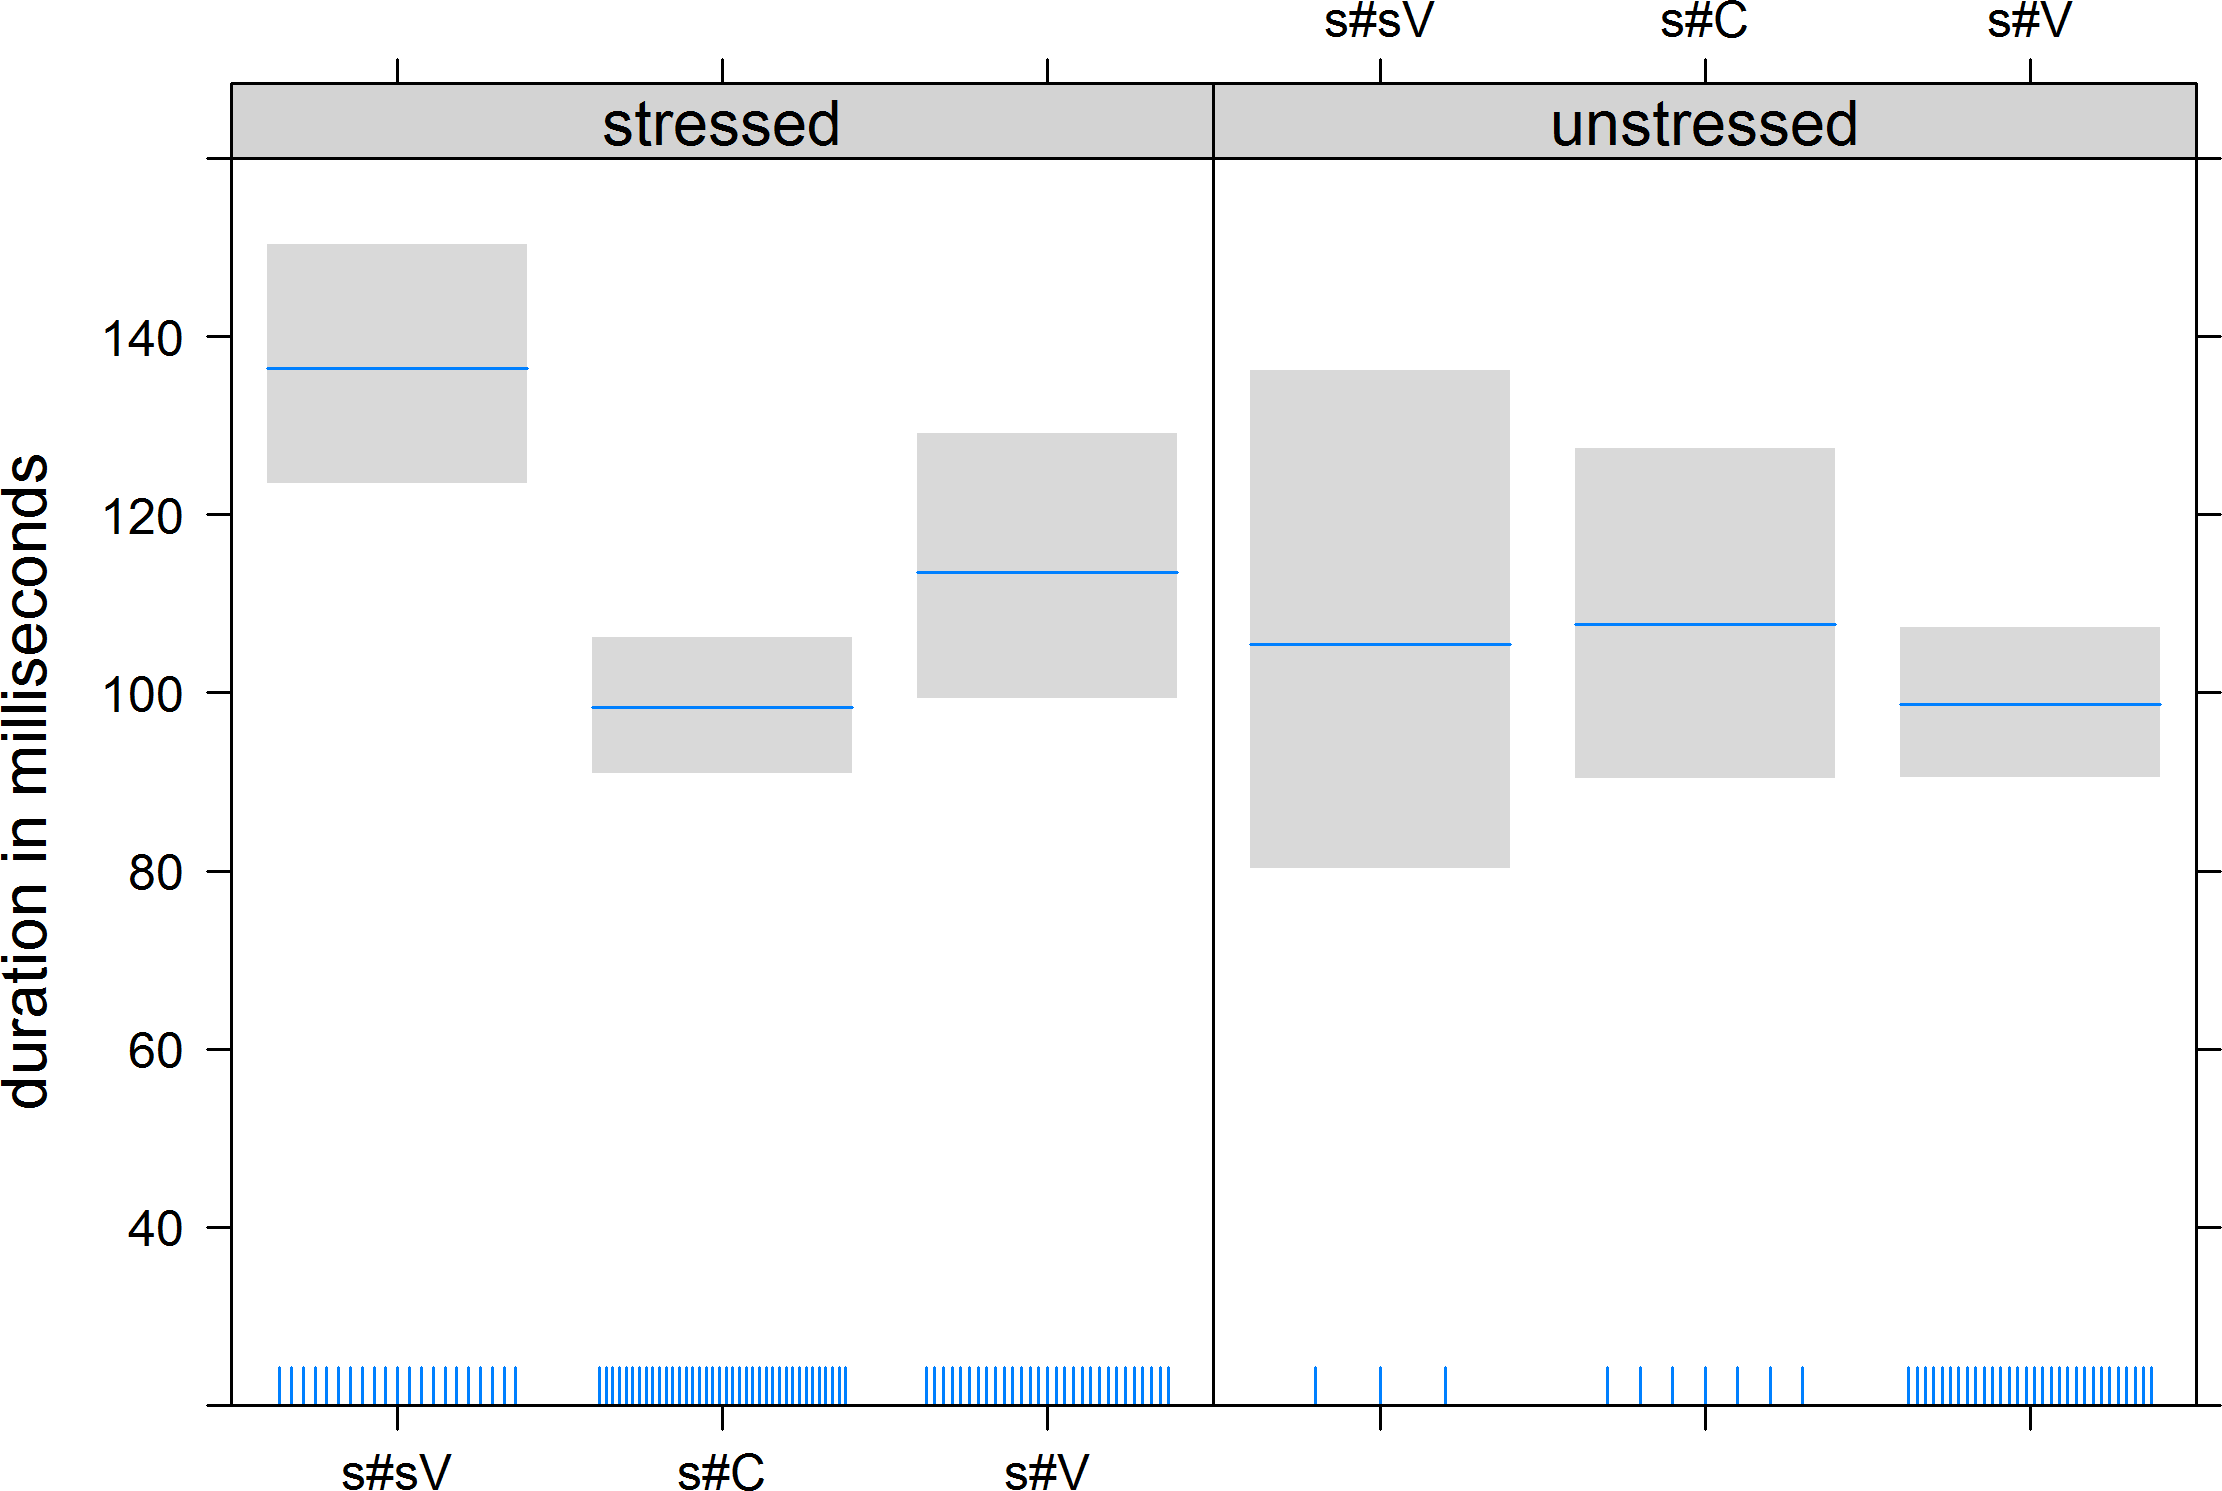
\includegraphics [scale=0.5]{images/Corpus/disModelTransitionTypeByStress.png}
	\caption{Effect of environment by base-initial stress on consonant duration in \prefix{dis}data set}
	\label{fig:corpus main effect 1 dis}
\end{figure*}

%Environment
The interaction between \textsc{Environment} and \textsc{BaseInitialStress} is displayed in \figref{fig:corpus main effect 1 dis}. The left panel of the figure displays the estimated effect of \textsc{Environment} on words with a \is{stress}stressed base-initial syllable. The right panel shows the estimated effect of \textsc{Environment} on words with an unstressed base-initial syllable. The figure shows that while there is a significant effect of \textsc{Environment} for words with a \is{stress}stressed base-initial syllable, there is no significant effect for words with an unstressed base-initial syllable. For words with a \is{stress}stressed base-initial syllable, doubles are estimated to be 38 ms  longer than singletons which are followed by a consonant, and 23 ms longer than singletons which are followed by a vowel. 
The difference in duration between the two singleton levels is marginally significant (p-value: $0.066$). The fricative before a consonant is predicted to be 15ms shorter than the fricative before a vowel.  There is no difference between the three environments for words with an unstressed base-initial syllable, i.e. doubles are of the same duration as singletons, and the two singleton levels are  also of the same duration. 


%



One could interpret the interaction between \textsc{Environment} and \textsc{BaseInitialStress} as evidence that the prefix \is{dis-}\prefix{dis} only geminates when followed by a \is{stress}stressed syllable, and that only in this condition the following segment, i.e. consonant or vowel, affects the duration of the prefixal consonant. However, there are two problems with the pertinent interaction, and the interpretation of the effects is therefore not that straightforward. Both problems are related to the distribution of variables in the data set. 

%first problem
The first problem is the number of types and tokens for each category. The blue lines on the bottom of the plot (in \figref{fig:corpus main effect 1 dis}), the rugs, indicate the number of tokens for each category. It is striking that there are only three tokens with an unstressed base-initial syllable and a double consonant at the morphological boundary. These three tokens are all of the same type, i.e. \textit{dissolution}. The interaction found in the model is hence caused by only three observations (of one type). In other words, there are only three tokens with a double consonant which do not geminate. All three tokens are of the type \textit{dissolution}. 

One might argue that the word \textit{dissolution} behaves differently because the word is simplex. There are two arguments for this assumption. First, \is{dis-}\prefix{dis} does not carry any meaning in the word \textit{dissolution}. Second, in the morphologically related derivative \textit{dissolve} the prefixal fricative is voiced. As discussed in \sectref{description un}, there are claims that voiced /s/ is only found in simplex \is{dis-}\prefix{dis}words. That the word \textit{dissolve} features a voiced fricative might thus indicate that it is lexicalized, which in turn might also mean that the related word \textit{dissolution} is lexicalized and no longer complex.

The second problem with the interaction  
is related to the distribution of the variable \textsc{Voicing}. 
 As already mentioned above, all voiced \is{dis-}\prefix{dis}prefixed words are semantically opaque, followed by a vowel and have a \is{stress}stressed base-initial syllable. The significant effect of \textsc{Voicing} in the final model is thus solely based on opaque, vowel-adjacent items with \is{stress}stressed base-initial syllables. Even though the effect is based on only a few items with a particular combination of features, the model accounts for \textsc{Voicing} in predicting consonant duration for all items of all levels. In other words, the model allocates the effect of \textsc{Voicing} to all levels irrespective of whether voiced items are actually present in the pertinent level. This might distort the effects of the affected variables, i.e. \textsc{SemanticTransparency}, \textsc{Environment} and \textsc{BaseInitialStress}. 
  With regard to the final model, the interaction between \textsc{Environment} and \textsc{BaseInitialStress} might be affected by this problem.
  Only two of the six pertinent categories feature voiced items, i.e. only words with base-initial \isi{stress} and a double consonant and words with base-initial \isi{stress} and a singleton followed by a vowel can be voiced. All other categories only feature voiceless items.
  
  
  
  To test whether the effects of \textsc{Environment} and \textsc{BaseInitialSyllable} are affected by the distribution of voiced items in the data set, and to also test the effect of \textsc{SemanticTransparency} without the possible harming influence of the variable \textsc{Voicing}, an additional model was fitted to the \is{dis-}\prefix{dis}data set. In this model only voiceless \is{dis-}\prefix{dis}prefixed words were included. The model included 104 observations, i.e. 24 voiced \is{dis-}\prefix{dis}prefixed words were excluded. 
  
  


 
\begin{table*}
	\caption{ Summary of linear model for variables predicting the Box-Cox-transformed duration of [s] in \prefix{dis}prefixed words with voiceless /s/}
	\label{tbl: summary model6}
	
					\resizebox{\textwidth}{!}{%		
		\begin{tabular}{lrrrr}
			
			
			\lsptoprule
			& Estimate & Std. Error & t-value & p-value  \\ 
			\midrule
			Intercept                             &0.716 &    0.017 &41.928 & $<$ 0.001\\	
			
			\textsc{Environment}-\texttt{s\#C}  &-0.050 &     0.009 &  -5.607 &$<$ 0.001\\ 
			
			\textsc{Environment}-\texttt{s\#V}   & -0.052 &   0.011 & -4.918 &$<$ 0.001 \\ 
			
			\textsc{SemanticTransparency}-\texttt{transparent}  &
			\color{lsLightGray}{-0.004 }& \color{lsLightGray} 0.008 & \color{lsLightGray}-0.523   &  \color{lsLightGray}0.602  \\ 
			
			\textsc{SpeechRate}  				  &-0.005 & 0.001 & -5.088   &$<$ 0.001 \\ 
			
			\textsc{BaseInitialStress}-\texttt{unstressed}   & -0.046 &   0.017 & -2.748 & 0.007 \\ 
			

			\textsc{SemanticTransparency}-\texttt{transparent}: &&&&\\
			\textsc{BaseInitialStress} - \texttt{unstressed}  & 0.052 &  0.020 & 2.646 & 0.010\\ 
			\midrule\\
			Adjusted R-squared: 0.375\\
			\lspbottomrule
		\end{tabular}
}
	
\end{table*}

The model predicting consonant duration with voiceless \is{dis-}\prefix{dis}prefixed words was fitted similarly to the model with all items. 
\tabref{tbl: summary model6} shows the final model for the voiceless fricatives. It explains about 38\% of the variance found in the data. 
As in the model with all \is{dis-}\prefix{dis}prefixed words, \textsc{LocalSpeechRate} has the expected effect on duration, and we find an effect of \textsc{BaseInitialStress} and \textsc{Environment}. However, in contrast to the complete model, in this model \textsc{BaseInitialStress} and \textsc{Environment} are not interacting. 
\figref{fig:corpus main effect 1 dis without voiced items} shows the effect of  \textsc{Environment}. One clearly sees that the double is predicted to be longer than both singleton consonants, irrespective of base-initial \isi{stress}. Furthermore, the durational difference between the two singleton levels is not significant in this model. One can hence assume that the marginally significant difference between the two singleton levels in the complete model was caused by the uneven distribution of voiced items in the complete \is{dis-}\prefix{dis}data set. 


\begin{figure*}
	
	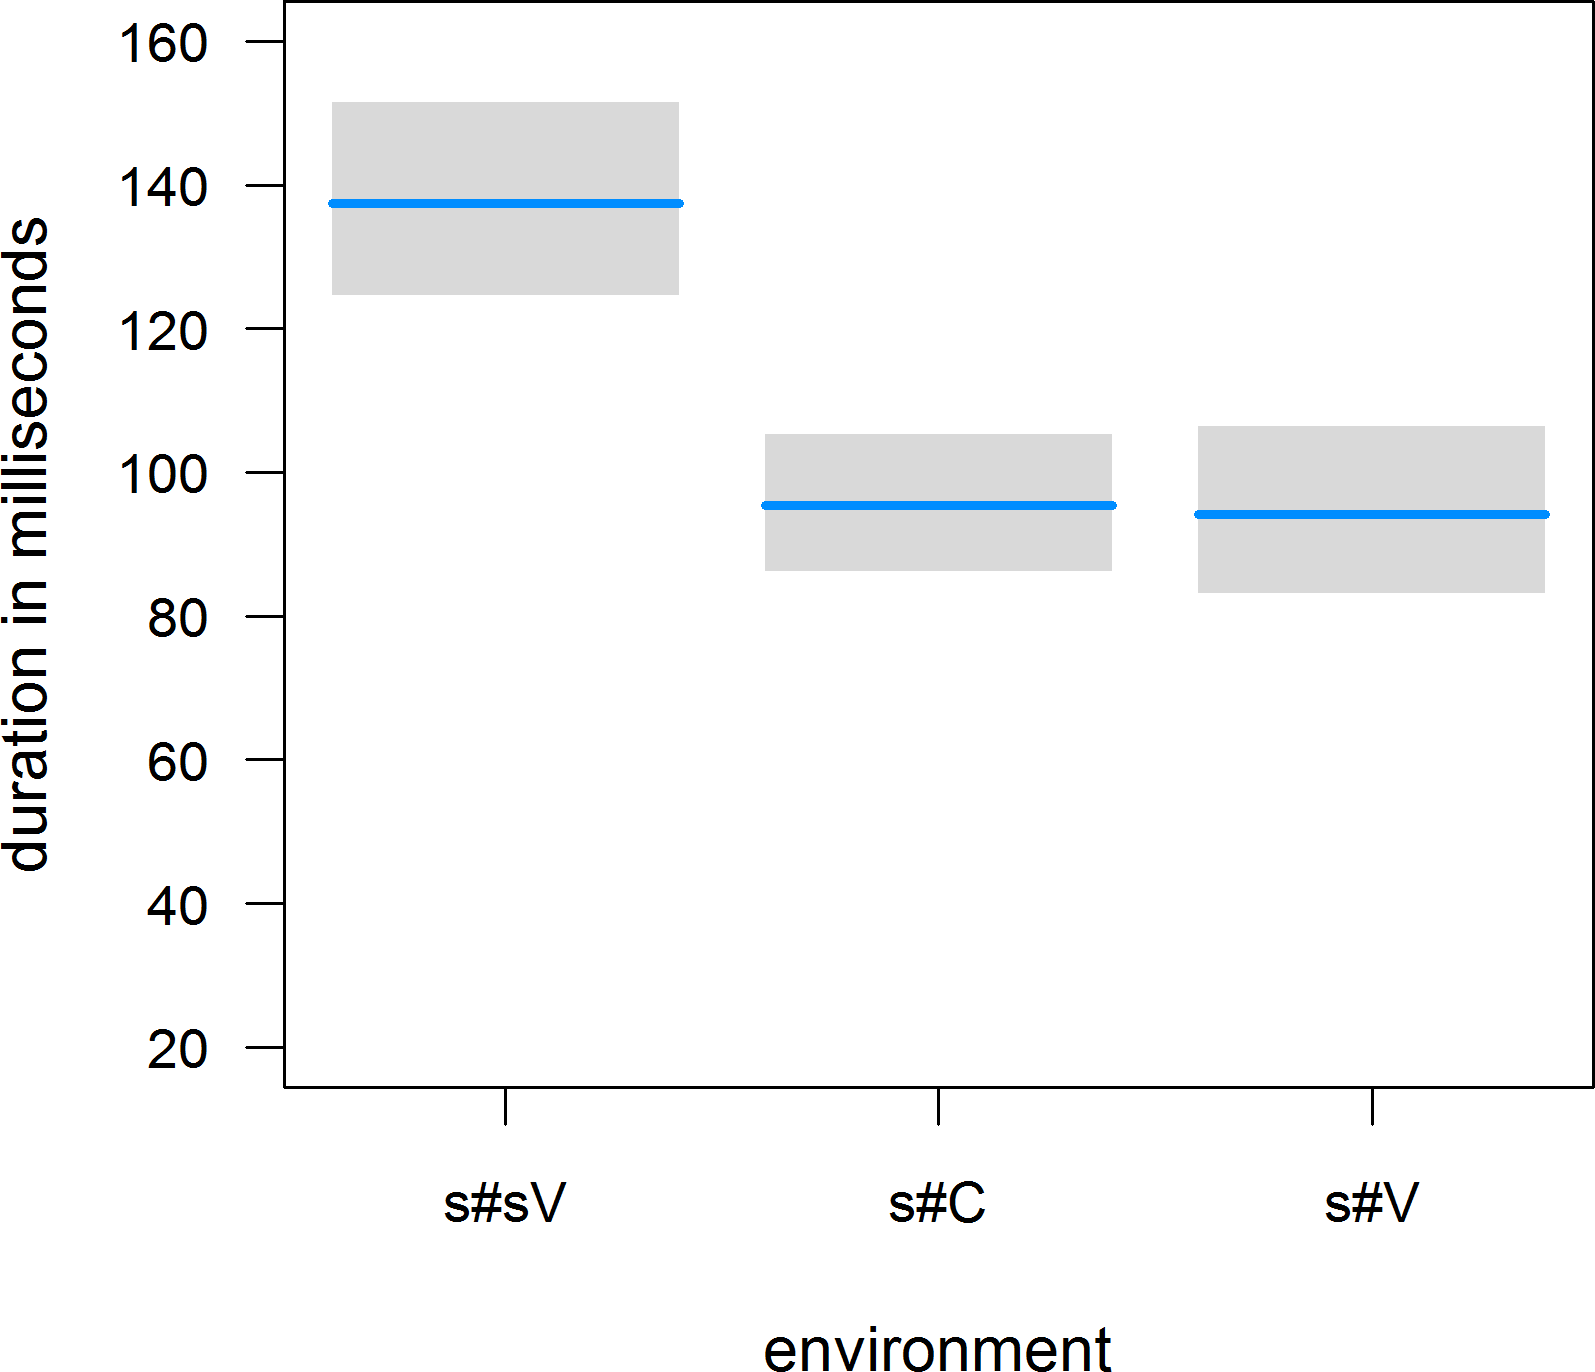
\includegraphics [scale=0.4]{images/Corpus/disModelWithoutVoicedSoundsEnvironment.png}
	\caption{ Effects of environment on consonant duration in voiceless \prefix{dis}data set}
	\label{fig:corpus main effect 1 dis without voiced items} 
\end{figure*}


\begin{figure*}
	

	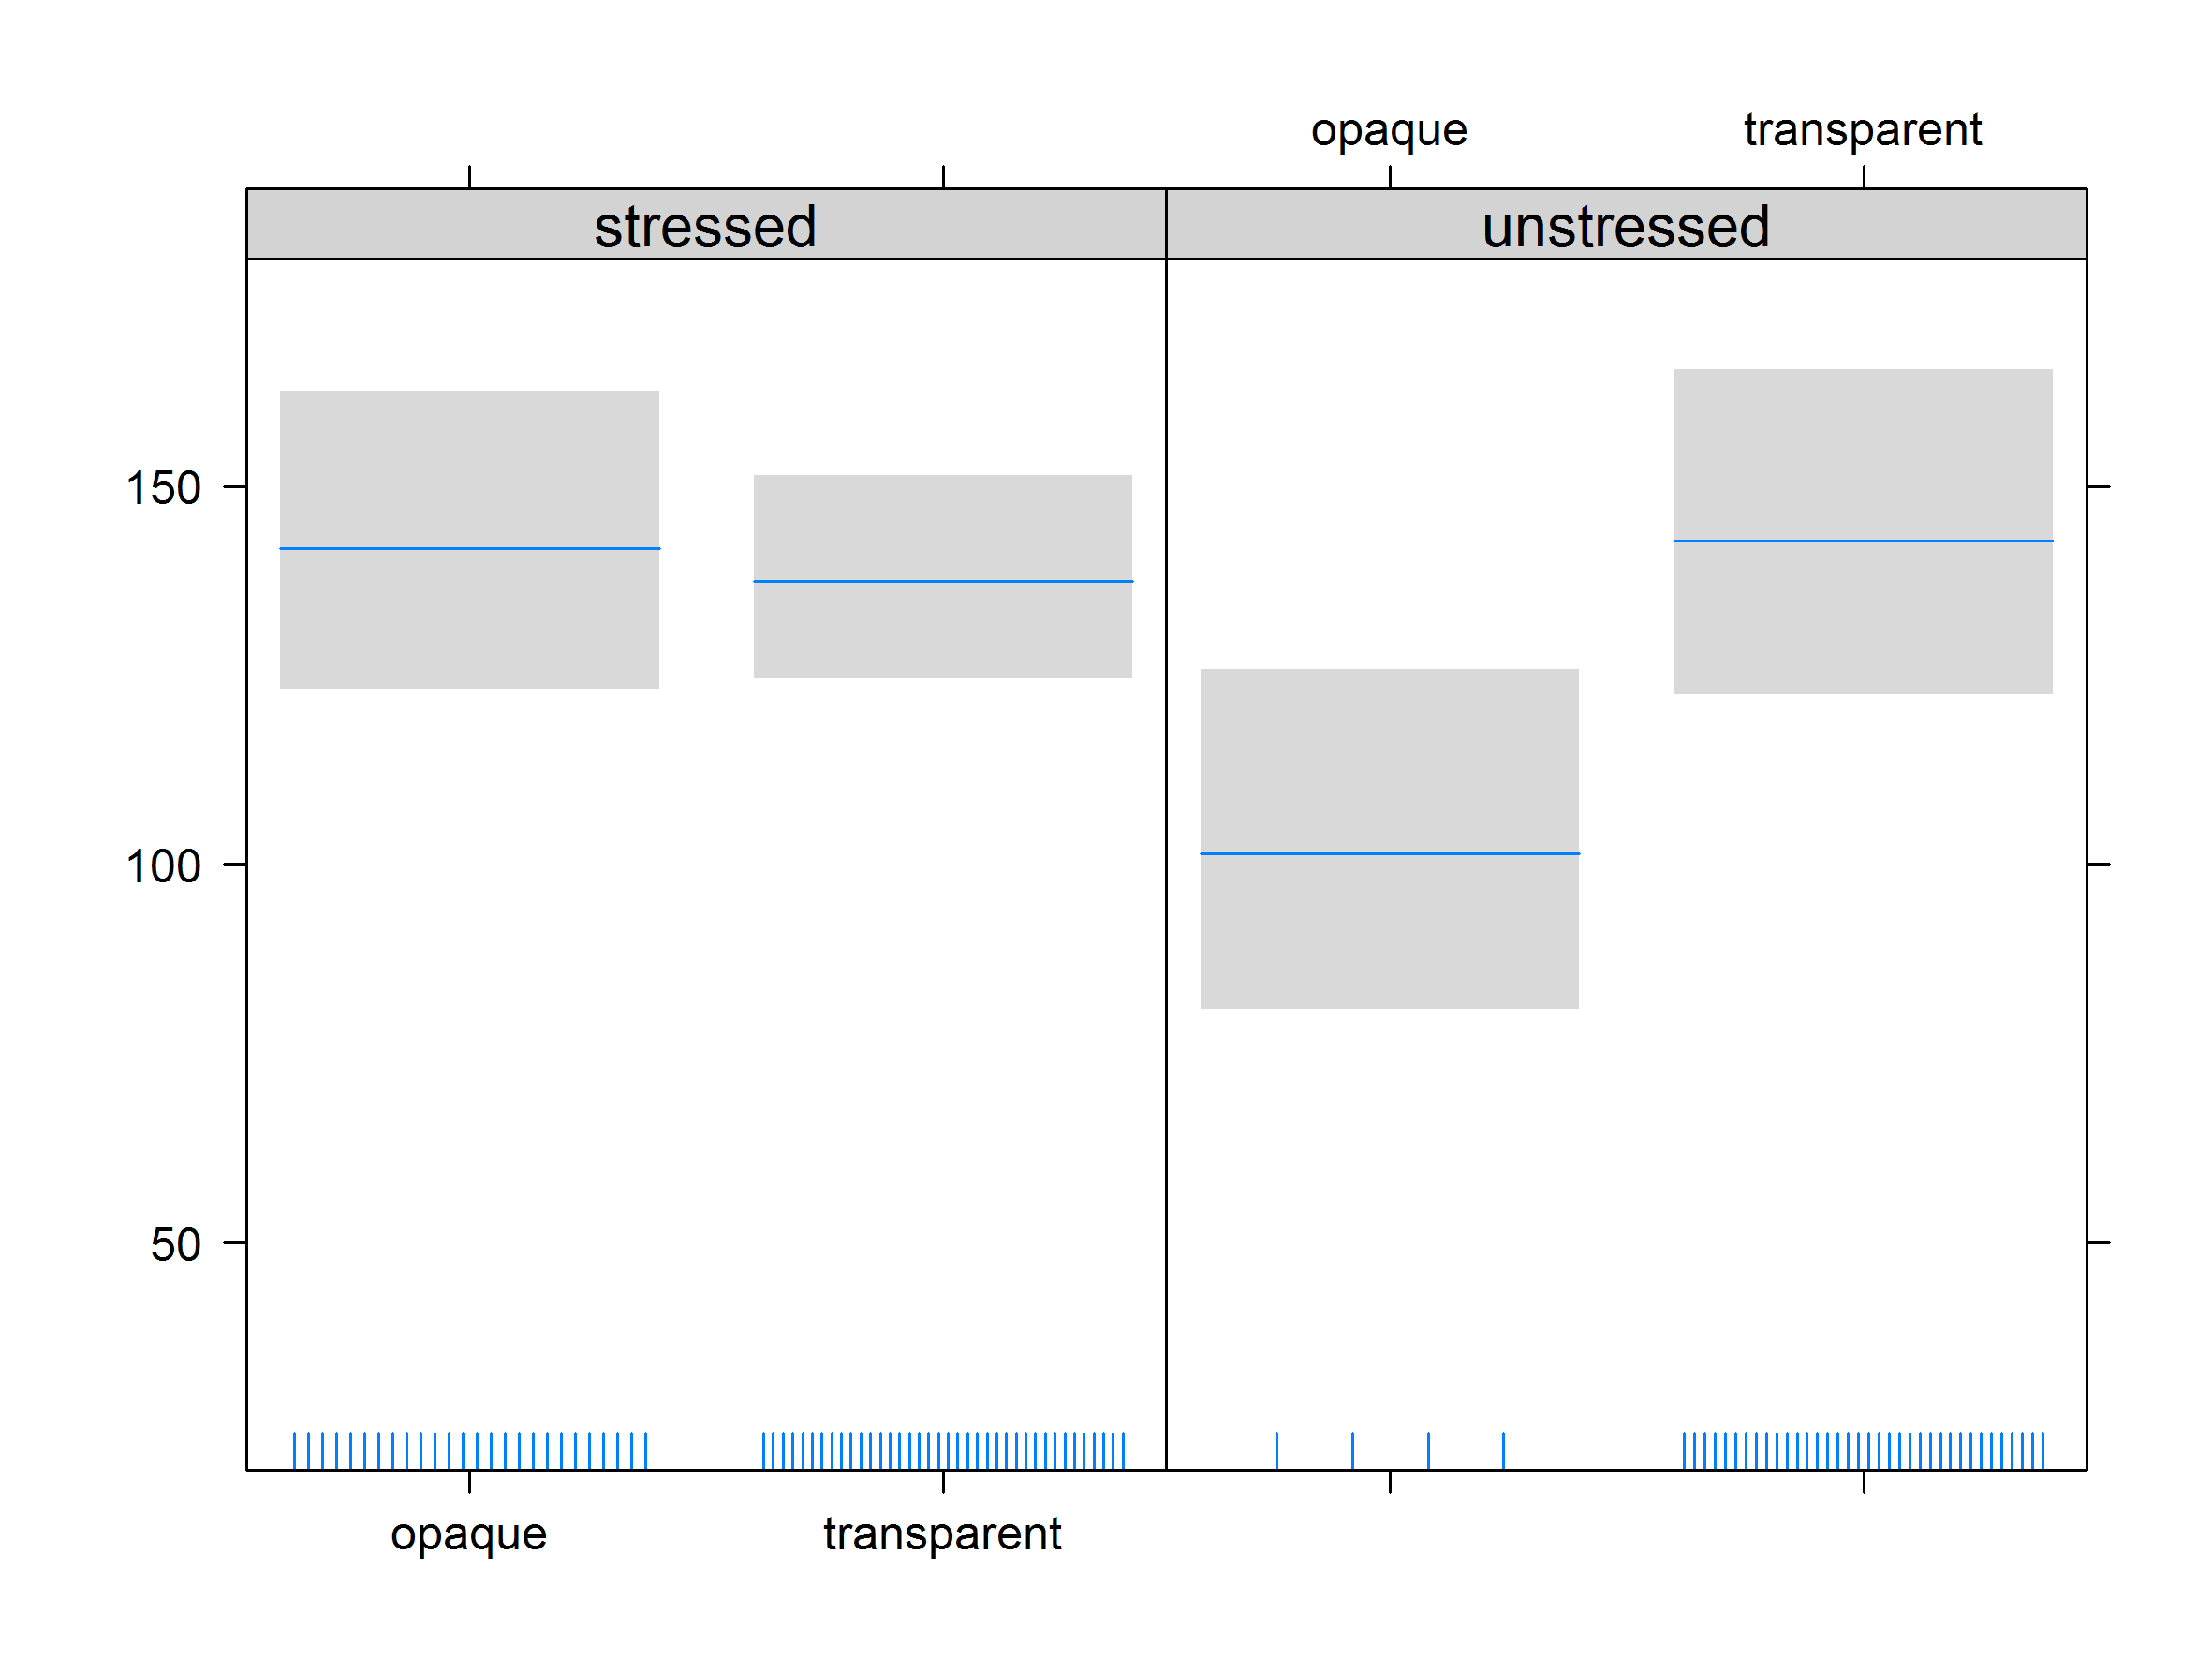
\includegraphics [scale=0.5]{images/Corpus/disModelWithoutVoicedSoundsSemanticTransTypeByStress.png}
	\caption{Effects of semantic transparency by  base-initial stress on consonant duration in voiceless \prefix{dis}data set}
	\label{fig:corpus main effect 2 dis without voiced items}
\end{figure*}






The voiceless model shows an interaction between the two variables \textsc{Semantic-Transparency} and \textsc{BaseInitialStress}. This interaction can be seen in \figref{fig:corpus main effect 2 dis without voiced items}. The left panel shows the effect of \textsc{SemanticTransparency} for items with a \is{stress}stressed base-initial syllable, the right panel shows the effect for items with an unstressed base-initial syllable. When the base-initial syllable is \is{stress}stressed, there is no difference between opaque and transparent items. When the base-initial syllable is unstressed, the fricative in opaque items is predicted to be 42 ms shorter than the fricative in transparent items. However, as in the complete model one must be cautious to  interpret this interaction. There are only four opaque tokens with an unstressed base-initial syllable in the data set. These four tokens cause the interaction, i.e. in these four tokens the fricative is significantly shorter than in all other tokens. 
Crucially, three of the four tokens are of the type \textit{dissolution}. This means that, even though we find two different interactions in the two \is{dis-}\prefix{dis}models (\textsc{BaseInitialStress} and \textsc{Environment} in the complete model vs. \textsc{BaseInitialStress} and \textsc{SemanticTransparency} in the voiceless model), the same tokens which cause the interaction in the complete model cause the interaction in the model with only voiceless items. It remains unclear whether the short fricative in the pertinent words is due to the unstressed base-initial syllable in combination with \isi{semantic opacity}, or whether the pertinent words behave differently because the \isi{stress} status of the base-initial syllable is crucial for \isi{gemination} with \is{dis-}\prefix{dis}, i.e. only words with a \is{stress}stressed base-initial syllable geminate, or whether the shorter fricative duration is caused by type-specific effects. 



After fitting a model with the individual \is{decomposability measure}decomposability measures, I fitted a model with combined \is{decomposability measure}decomposability measures. The combined measures were created by means of a \is{principal component analysis}principal component analysis (cf. \sectref{stats} on \is{principal component analysis}principal component analyses). 
The \is{principal component analysis}principal component analysis included the four variables log\textsc{RelativeFrequency}, \textsc{SemanticTransparencyRating}, \textsc{TypeOfBase} and \textsc{SemanticTransparency}. As with \is{in-}\prefix{in}, the variable \textsc{LSAScore} was not included in the \is{principal component analysis}principal component analysis as it would have led to an extreme \isi{reduction} of the data set. Categorical variables were recoded as numerical before they entered the analysis, and all variables were scaled.




\tabref{tbl: summary PC discorpus} shows a summary of the principal components. The first \is{principal component analysis}principal component accounts for most of the variance and is composed more or less equally of all measures. The second component is dominated by \textsc{TypeOfBase} and log\textsc{RelativeFrequency}, the third component mostly represents \textsc{SemanticTransparency}, \textsc{TypeOfBase} and log\textsc{RelativeFrequency}, and the fourth is mostly composed of \textsc{SemanticTransparency} and \textsc{SemanticTransparencyRating}. The second and the third component explain much less variance than the first, and the last \is{principal component analysis}principal component explains barely any variance. The first three principal components were included in the model.



After model simplification none of the principal components remained in the model. The final model resembles the final model of the complete data set. This means that the four variables \textsc{Environment}, \textsc{LocalSpeechRate}, \textsc{Voicing} and \textsc{BaseInitialStress} proved to be significant, and that \textsc{Environment} and \textsc{BaseInitialStress} form an interaction in the model. Decomposability did not affect fricative duration. 


\begin{table*}
	\caption{ Summary of principal components}
	\label{tbl: summary PC discorpus}
	
		\resizebox{\textwidth}{!}{%		
			\begin{tabular}{lrrrr}
				
				
				\lsptoprule
				
				
				\multicolumn{5}{l}{\textbf{Composition of principal components}}\\
				
				&PC1&          PC2 &       PC3       & PC4   \\
				\midrule
				
				scaled\textsc{RelativeFrequency } &  0.449&  0.653 & 0.609& 0.036\\ 
				scaled\textsc{SemanticTransparencyRating}  &   0.563 &-0.094 &-0.269& -0.776\\
				scaled\textsc{TypeOfBase }&0.441& -0.735 & 0.447  & 0.255\\
				scaled\textsc{SemanticTransparency }& 0.535  &0.158 &-0.598 &  0.576\\
				\midrule
				\multicolumn{5}{l}{\textbf{Variance explained by principal components}}\\
				&PC1&          PC2 &       PC3       & PC4  \\
				\midrule
				Proportion of Variance &0.679& 0.174& 0.105& 0.042\\
				\lspbottomrule
			\end{tabular}
		}
	
\end{table*}

%Mumin voiced
Two \isi{multi-model inferencing} analyses were conducted for \is{dis-}\prefix{dis}, one for the complete data set, one for the voiceless data set. As with \is{in-}\prefix{in}, the principal components were used to test the predictive value of the \is{decomposability measure}decomposability variables. In other words, to avoid \isi{collinearity} problems, the principal components were used in the analyses instead of the individual \is{decomposability measure}decomposability measures. 

The models revealed that \textsc{LocalSpeechRate} and \textsc{Environment}  are the most important variables in both models (importance value: $1$). In the complete model, \textsc{Voicing} was also of high importance (importance value: $1$). 
For both data sets, \textsc{BaseInitialStress} proved to be the next most important variable. However, its importance value is much lower than the ones of \textsc{Environment}, \textsc{LocalSpeechRate} and \textsc{Voicing} ($0.47$ in complete model, $0.32$ in voiceless model).
 All other variables were much less important in both models. 
The importance values for the complete model are $0.37$ for log\textsc{WordFormFrequency},  $0.26$ for \textsc{PrecedingSegmentDuration}, $0.29$ for \textsc{PC2}, $0.25$ for \textsc{PC1},  and $0.25$ for \textsc{PC3}; 
 the importance values for the voiceless model are $0.30$ for \textsc{PC3}, $0.28$ for log\textsc{WordForm-Frequency}, $0.28$ for \textsc{PC1}, $0.27$ for \textsc{PC2} and $0.30$ for \textsc{PrecedingSegmentDuration}.



\subsubsection{Relative duration}

In the model predicting \isi{relative duration} with \is{dis-}\prefix{dis}, the residuals showed a normal distribution and therefore no transformation of the dependent variable was necessary. The model was fitted similarly to the \isi{absolute duration} model, i.e. \is{decomposability measure}decomposability measures were tested individually, as well as in terms of principal components, and the same interactions were tested. Let us first discuss the model with the individual \is{decomposability measure}decomposability measures.

After model simplification, the following four variables remained in the final model: \textsc{Environment}, \textsc{SemanticTransparency}, \textsc{Voicing} and \textsc{BaseInitialStress}. With an adjusted R-squared of $0.262$ the model explains less of the variance than the \isi{absolute duration} model. The model summary is printed in \tabref{tbl: summary model5}.
  
    \begin{table*}
    	\caption{ Summary of linear model for variables predicting the relative  duration of [s] in \prefix{dis}prefixed words}
    	\label{tbl: summary model5}
    	
    					\resizebox{\textwidth}{!}{%		
    		\begin{tabular}{lrrrr}
    			\lsptoprule
    			& Estimate & Std. Error & t-value & p-value  \\ 
    			\midrule
    			Intercept                             & 1.937 &   0.231  & 8.384 &$<$ 0.001\\	
    			
    			\textsc{Environment}-\texttt{s\#C}  & -0.838  &   0.203 &-4.134  &$<$ 0.001\\ 
    			
    			\textsc{Environment}-\texttt{s\#V}   &-0.643 & 0.208 &-3.089 & 0.002\\ 
    			
    			\textsc{SemanticTransparency}-\texttt{transparent}				   & -0.390 &   0.194 &-2.015 &0.046\\ 
					
    			\textsc{Voicing}-\texttt{voiceless}   &1.187 &0.281 &  4.225  & $<$ 0.001 \\ 	
    			
    			
    			\textsc{BaseInitialStress}-\texttt{unstressed}   &-0.370 &  0.185  & -1.998  &0.048 \\ 

    			\midrule\\
    			Adjusted R-squared: 0.262\\
			\lspbottomrule
    		\end{tabular}
    	}
    	
    \end{table*}
  
The variable \textsc{Voicing} shows the same effect as in the \isi{absolute duration} model. Voiced fricatives are shorter than voiceless fricatives.
The effects of \textsc{Environment} and \textsc{BaseInitialStress} are also similar to the ones found in the \isi{absolute duration} model. Doubles are longer than singletons, and consonants are shorter before unstressed base-initial syllables than before \is{stress}stressed base-initial syllables. 
In contrast to the \isi{absolute duration} model, the \isi{relative duration} model does not show an interaction between \textsc{Environment} and \textsc{BaseInitialStress}, or between \textsc{SemanticTransparency} and \textsc{BaseInitialStress}. This means that, in contrast to the \isi{absolute duration} model,  all \is{dis-}\prefix{dis}prefixed types geminate in terms of their \isi{relative duration}. Furthermore, all prefixal fricatives are affected by an unstressed base-initial syllable, i.e. not just opaque words or words with a double consonant.

The effect of \textsc{BaseInitialStress} on \isi{relative duration} with \is{dis-}\prefix{dis} deviates from the effect of \textsc{BaseInitialStress} on \isi{relative duration} with \is{in-}\prefix{in}. For \is{in-}\prefix{in}, we find shorter relative durations before \is{stress}stressed syllables than before unstressed syllables. This effect was explained by reference to the preceding vowel duration in \is{in-}\prefix{in}. There are different possibilities for the deviating results between \is{in-}\prefix{in} and \is{dis-}\prefix{dis}. It might for example be that inherent durational differences between the consonants, i.e. /m/ vs. /s/, led to different results. Another possibility is that preceding vowel durations differ between \is{in-}\prefix{in} and \is{dis-}\prefix{dis}.
          

 The final \isi{relative duration} model shows a significant effect of \textsc{SemanticTrans-parency}. Transparent items are predicted to have shorter fricatives than opaque items. This is an unexpected effect, which is not found in \isi{absolute duration}, and one must be cautious to interpret the effect. 
 As discussed above, there is a close and complex relation between the variables \textsc{Voicing} and \textsc{SemanticTransparency}. This relation might have caused the surprising result. To see whether this is the case, an additional model with only voiceless items was fitted. The model is displayed in \tabref{tbl: summary model7}.
 With an R-squared of $0.204$, the model explains 20\% of the data. This is less than any other model fitted to the \is{dis-}\prefix{dis}data set. Only one variable remained significant in the model, \textsc{Environment}. The fricative in \texttt{s\#sV}-structures is longer than the fricative in \texttt{s\#C}- and \texttt{s\#V}-structures. In other words, the model again shows that \is{dis-}\prefix{dis} geminates. 
 Crucially, \textsc{SemanticTransparency} does not reach significance in the model. One can therefore conclude that the effect found in the complete model is probably caused by the distribution of voicing in the data set. In other words, the effect is not stable and therefore not trustworthy.

    \begin{table}
    	\caption{ Summary of linear model for variables predicting the relative  duration of [s] in \prefix{dis}prefixed words with voiceless /s/}
    	\label{tbl: summary model7}
    	
    					\resizebox{\textwidth}{!}{%		
    		\begin{tabular}{lrrrr}
    			\lsptoprule
    			& Estimate & Std. Error & t-value & p-value  \\ 
    			\midrule
    			Intercept                             & 2.878   &  0.172 & 16.692  & $<$ 0.001 \\	
    			
    			\textsc{Environment}-\texttt{s\#C}  & -0.823 &  0.207&  -3.970 &  $<$ 0.001\\ 
    			
    			\textsc{Environment}-\texttt{s\#V}   &-1.123  &   0.212&  -5.295 &$<$ 0.001 \\
    			
    			
    			\midrule\\
    			Adjusted R-squared: 0.204 \\
			\lspbottomrule
    		\end{tabular}
    	}
    	
    \end{table}



After fitting the model with the individual \is{decomposability measure}decomposability measures, the model with the principal components was fitted. After simplification, the principal component model showed similar effects as the model with the individual \is{decomposability measure}decomposability measures (see \tabref{model im PC Corpus abs} in \hyperref[Appendix D: model summaries corpus]{appendix D} for model summary). The effects of \textsc{Environment} and \textsc{Voicing} are identical. However, instead of the variables \textsc{BaseInitialStress} and \textsc{SemanticTransparency}, this model includes the variable \textsc{PC1}. 
The effect of \textsc{PC1} is shown in \figref{fig:PC1 dis Corpus}. 


\begin{figure*}
	
	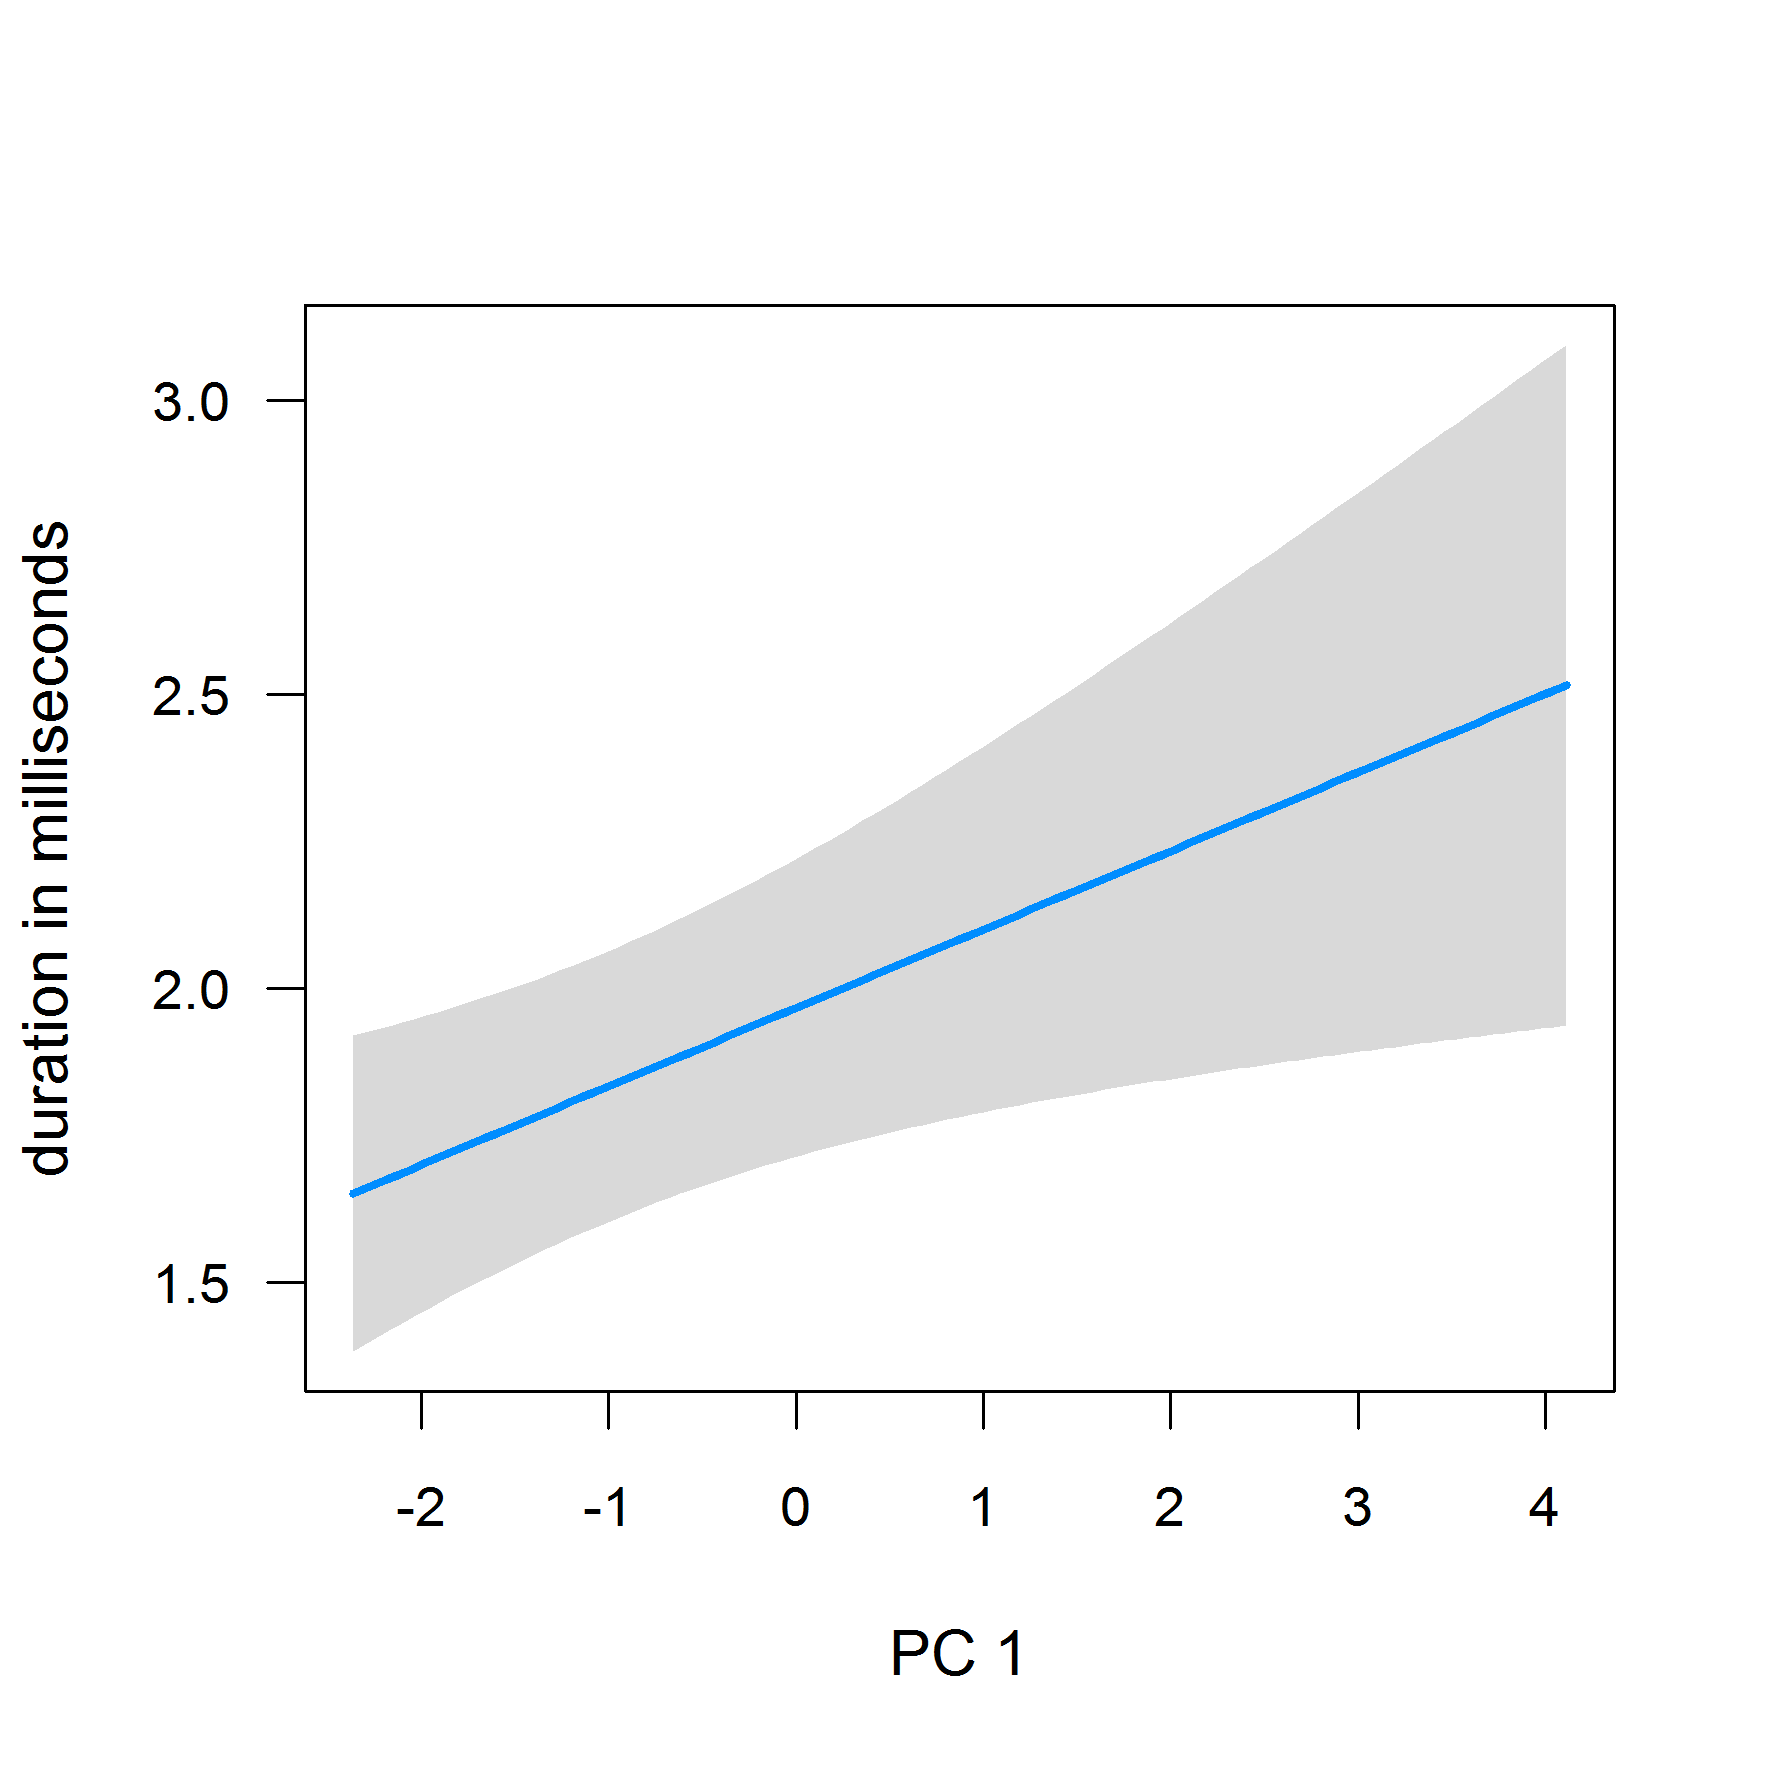
\includegraphics [scale=0.4] {images/Corpus/disPCAbsPC4.png}
	\caption{Effect of PC1 on relative consonant duration in complete \prefix{dis}data set}
	\label{fig:PC1 dis Corpus}
\end{figure*}


The higher the value of \textsc{PC1}, the longer the \isi{relative duration} of the fricative. As explained above, \textsc{PC1} is composed of all \is{decomposability measure}decomposability measures. The higher the \textsc{PC1}-value, the less decomposable a word is.
 One can thus interpret the effect of \textsc{PC1} in the following way: the less decomposable a derivative, the longer the \isi{relative duration} of /s/. This is unexpected with regard to the \isi{decomposability} predictions. It is, however, somewhat expected with regard to the results from the complete \isi{relative duration} model, in which \is{semantic transparency}semantically transparent words are predicted to have shorter fricatives than semantically opaque words. As discussed above, this effect might be caused by the distribution of certain properties among types and tokens in the subset, and one must therefore be cautious with the interpretation of the effect. All in all, one can state that the principal component model shows similar effects as the model with the individual \is{decomposability measure}decomposability measures, and that the interpretation of the \isi{decomposability} effect is yet unclear.






As for \isi{absolute duration}, two \isi{multi-model inferencing} analyses were conducted to identify the most important variables for predicting \isi{relative duration} with \is{dis-}\prefix{dis}, one for the complete data set and one for the voiceless data set. 
 As in the \isi{absolute duration} models, \textsc{Environment} is clearly the most important variable in both models (importance value: $1$). In the complete model, \textsc{Voicing} is also of very high importance  (importance value: $0.99$). For both data sets, the first \is{principal component analysis}principal component (\textsc{PC1}) reaches a rather high importance value (complete data set: $0.85$,  voiceless data set: $0.71$). The importance values of all other variables are much lower.
\textsc{BaseInitialStress} has an importance value of $0.56$ in the complete data set and one of $0.41$ in the voiceless data set,   
\textsc{PC2} has an importance value of $0.47$ in the complete data set and one of $0.40$ in the voiceless data set,   
\textsc{PC3} has an importance value of $0.27$ in the complete data set and one of $0.28$ in the voiceless data set,   
log\textsc{WordFormFrequency} has an importance value of $0.27$ in the complete data set and one of $0.25$ in the voiceless data set, and  
\textsc{LocalSpeechRate} has an importance value of $0.26$ in the complete data set and one of $0.24$ in the voiceless data set.  

\subsubsection{Summary}


The models predicting \isi{absolute duration} with \is{dis-}\prefix{dis} and the models predicting \isi{relative duration} with \is{dis-}\prefix{dis} reveal similar effects. In general, all models feature the same set of variables, and there are only small differences between the models. The models predicting \isi{relative duration} feature fewer significant variables, and only in \isi{absolute duration} models interactions were found to be significant. 
The \isi{absolute duration} models feature a higher R-squared than the \isi{relative duration} models. They thus explain more of the variance in the data than the \isi{relative duration} models. This finding is similar to what was found for \is{un-}\prefix{un} and \is{in-}\prefix{in}. 

%Loc Speech 
With regard to the noise variables, \textsc{LocalSpeechRate}, \textsc{Voicing}  and \textsc{BaseInitialStress} had a significant effect on consonant duration in the models. 
In \isi{absolute duration}, \textsc{LocalSpeechRate} influenced fricative duration in the expected direction, i.e. the higher the \isi{speech rate}, the shorter the fricative. \textsc{LocalSpeechRate} did not affect the \isi{relative duration} of the fricative. 
An effect of \textsc{Voicing} was found in the two models containing all \is{dis-}\prefix{dis}prefixed items, i.e. voiced and voiceless items. Voiced items are shorter than voiceless items in absolute and \isi{relative duration}.
The effect of \textsc{BaseInitialStress} is less clear. While in \isi{relative duration}, an unstressed base-initial syllable leads to the shortening of the fricative in all \is{dis-}\prefix{dis}prefixed words, in the \isi{absolute duration} models the variable forms interactions. In the model with only voiceless items \textsc{BaseInitialStress} interacts with \textsc{SemanticTransparency},  in the complete model it interacts with \textsc{Environment}.



% The two interactions
Both interactions with the variable \textsc{BaseInitialStress} are caused by only few tokens in the data set, three in the complete model and four in the voiceless model. Three of those tokens are of the type \textit{dissolution}, which is the only type in the data set which is opaque, features a double consonant and has an unstressed base-initial syllable. 
In the voiceless model, we find that in opaque items with an unstressed base-initial syllable, i.e. in the three tokens of the type \textit{dissolution} and in the one token of the type \textit{discount}, consonants are shorter than in all other items. 
In the complete model, we find that doubles in words with an unstressed base-initial syllable, i.e. doubles in the type \textit{dissolution}, are shorter than in all other double consonant items. They are as long as singletons. This means that while all other double consonants geminate, the double consonant in these words is not significantly longer than a singleton.

The two \isi{absolute duration} models thus predict particularly short fricative durations for the same tokens, in particular tokens of the type \textit{dissolution}. The models differ, however, in how they explain the shortness of the consonant. While in the complete model the short double consonant is explained by the following unstressed syllable, in the voiceless model it is explained by the combination of an unstressed base-initial syllable with \isi{semantic opacity}. It remains unclear whether the short duration of /s/ in \textit{dissolution} is caused by its unstressed base-initial syllable, i.e. whether all \is{dis-}\prefix{dis}prefixed words degeminate when followed by an unstressed syllable, or whether it is caused by the combination of an unstressed base-initial syllable and \isi{semantic opacity}, or whether this is a type-specific effect.


All in all, the analyses suggest that, in general, \is{dis-}\prefix{dis} geminates. Except for the complete \isi{absolute duration} model, in which one type with a double consonant degeminates, i.e. \textit{dissolution}, all  models show a robust effect of the variable \textsc{Environment}. In both absolute and \isi{relative duration}, doubles are significantly longer than singletons. There is no significant difference in duration between the two singleton levels. Furthermore, \isi{multi-model inferencing} supports the claim that \is{dis-}\prefix{dis} geminates by showing the importance of the variable \textsc{Environment} for all models. 
One can thus summarize that the corpus study shows that in the majority of cases, the prefix \is{dis-}\prefix{dis} geminates. The only \is{dis-}\prefix{dis}prefixed word in the data set which might degeminate is the word \textit{dissolution}.

With regard to the other variables of interest, i.e. the \is{decomposability measure}decomposability measures, only \textsc{SemanticTransparency} showed a significant effect in \isi{absolute duration}. The effect was only significant in one model and formed an interaction with \textsc{BaseInitialStress}. As discussed above, the interaction is  caused by only a few items and therefore difficult to interpret.
 In the \isi{relative duration} models, effects of \textsc{SemanticTranspaency} and \textsc{PC1} were found. Due to the distribution of certain properties in the data set, these effects are, however, also difficult to interpret. 


\subsection{The suffix \suffix{ly}}


\subsubsection{Absolute duration}

After the exclusion of two outliers, the \is{-ly}\suffix{ly}-model showed a satisfactory distribution of residuals, and an initial model was fitted. 
With regard to \isi{decomposability}, only the two \is{decomposability measure}decomposability measures \textsc{LSAScore} and log\textsc{RelativeFrequency} were tested in the model. As described in \sectref{The decomposability of the four affixes: a comparison}, in the \is{-ly}\suffix{ly}-data set the variables \textsc{SemanticTransparency}, \textsc{TypeOfBase}  and \textsc{SemanticTransparencyRat-ing} did not show any, or barely any, variation. Therefore, their effect on consonant duration in \is{-ly}\suffix{ly} could not be tested. The variable \textsc{PrecedingSegmentDuration} was also discarded. This was because of its high correlation with the variable \textsc{PrecedingSegment}, which would have caused \isi{collinearity} problems in the model. In preliminary analyses, the variable \textsc{PrecedingSegment} proved to be the better predictor. Therefore, this variable was used in the model and not \textsc{PrecedingSegmentDuration}. 

The model for the \textit{ly-}data set was simplified according to the same procedure as the  previous models. A list of all tested interactions in the model can be found in \hyperref[Appendix C: Summaries of tested interactions in corpus study]{appendix C}. 
The final model is summarized in \tabref {tbl: corpus summary model ly}.


\begin{table*}
	\caption{Summary of linear model for variables predicting the  duration of [l] in \suffix{ly}-suffixed words}
	\label{tbl: corpus summary model ly}
	
					\resizebox{\textwidth}{!}{%		
		
		\begin{tabular}{lrrrr}
			
			
			\lsptoprule
			& Estimate & Std. Error & t-value & p-value  \\ 
			\midrule
			Intercept                           &   77.323& 8.438 & 9.163& $<$0.001\\
			\textsc{Environment}-\texttt{\is{syllabicity}syllabic l\#l} &
			\color{lsLightGray} {7.387}  & \color{lsLightGray} 5.641 &\color{lsLightGray}1.309 &\color{lsLightGray} 0.192 \\
			\textsc{Environment}-\texttt{\#l} &
			\color{lsLightGray} {3.965} & \color{lsLightGray}  4.761 &\color{lsLightGray}0.833  & \color{lsLightGray}0.406 \\
			\textsc{LocalSpeechRate} &                 -2.335 &  0.438 & -5.332& $<$0.001\\
			\textsc{PrecedingSegment} - \texttt{vowel}  &    15.694  &4.429&  3.544  & 0.001\\
				log\textsc{WordFormFrequency} &       -1.631&0.777 &  -2.100 & 0.038 \\		
			\midrule\\
			Adjusted R-squared: 0.236\\
			\lspbottomrule

		\end{tabular}
	}
	
\end{table*}





The model explains about 24\% of the variance and features four variables of which three are significant. The three noise variables \textsc{LocalSpeechRate}, \textsc{PrecedingSegment} and log\textsc{WordFormFrequency} are significant. 
The variable \textsc{Environment} does not show a significant effect but remained in the model as it is the crucial variable with regard to \isi{gemination}.



\figref{fig:corpus covariates ly} displays the effects of \textsc{LocalSpeechRate} and \textsc{PrecedingSegment}. The left panel of the figure shows that with increasing \isi{speech rate} /l/ becomes shorter, and the right panel shows that after a vowel /l/ is longer than after a consonant. These effects are expected.





\begin{figure*}
	
		
	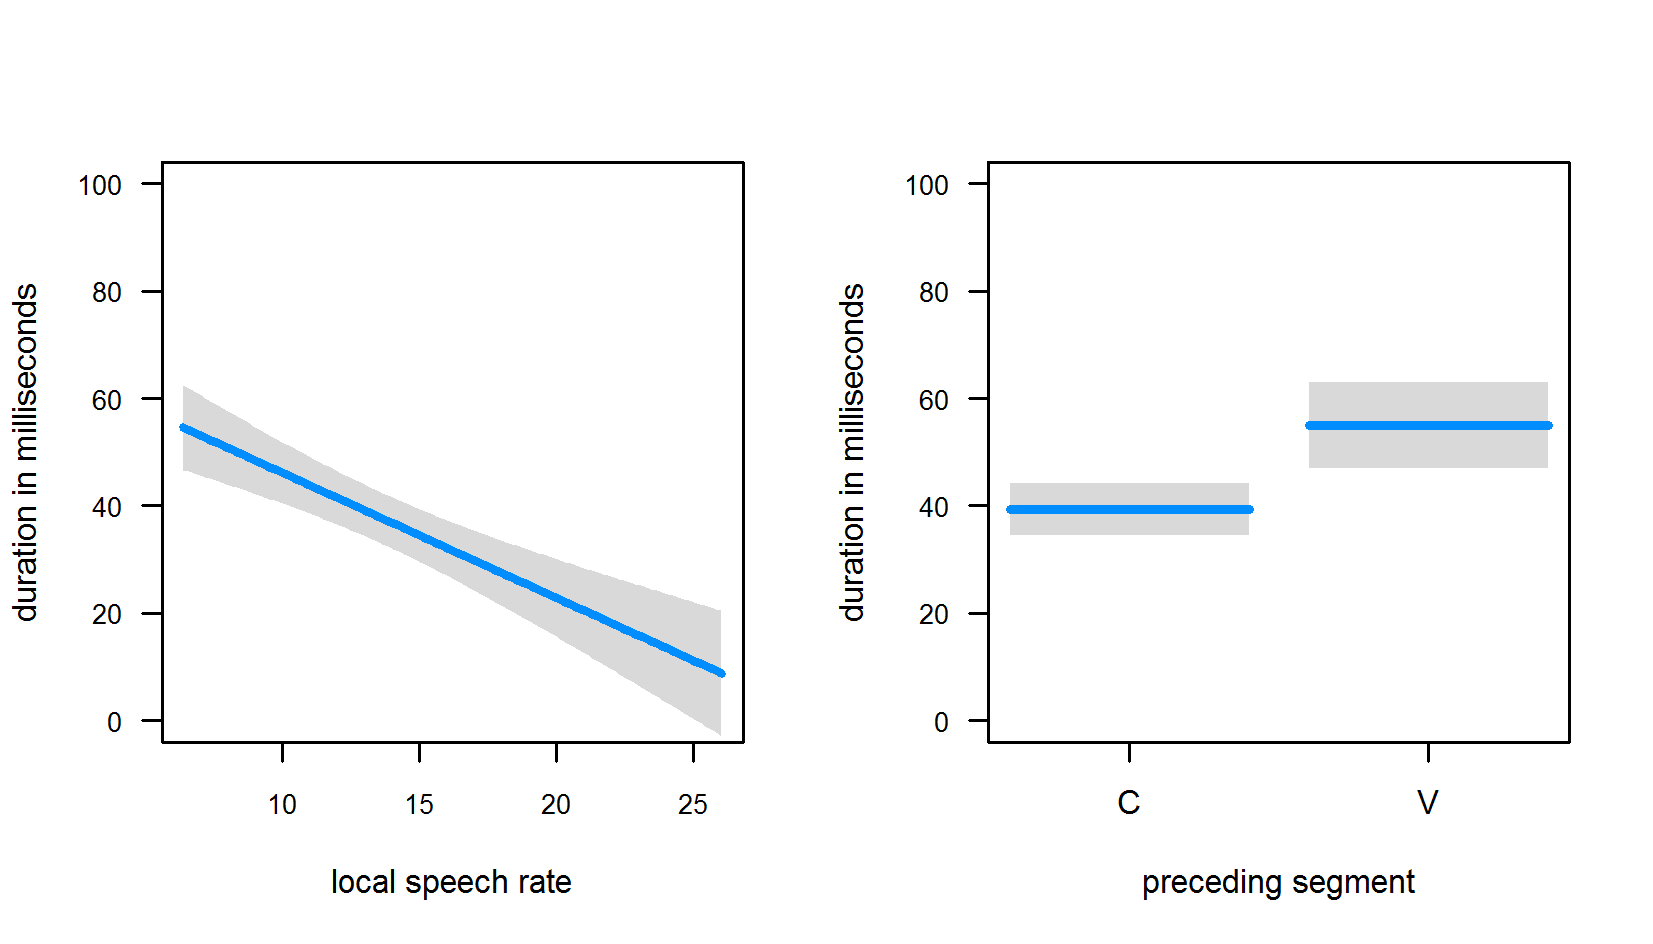
\includegraphics[scale=.8] {images/Corpus/lyModelcov.png}
	\caption{Effects of local speech rate and preceding segment on consonant duration in \suffix{ly}-data set}
	\label{fig:corpus covariates ly}
\end{figure*}





\figref{fig:corpus main effects  ly} shows the effects of log\textsc{WordFormFrequency} and \textsc{Environment}.
The left panel of the figure shows that with increasing \isi{frequency} /l/ becomes shorter. This is expected.
The right panel of the figure shows the insignificant effect of \textsc{Environment} on consonant duration in \is{-ly}\suffix{ly}. The figure clearly shows that there is no durational difference between double /l/ (\texttt{l\#l}), \is{syllabicity}syllabic double /l/ (\is{syllabicity}syllabic \texttt{l\#l}) and singleton /l/ (\texttt{\#l}). The suffix \is{-ly}\suffix{ly} thus clearly degeminates in \isi{absolute duration}. 


\begin{figure*}
	

	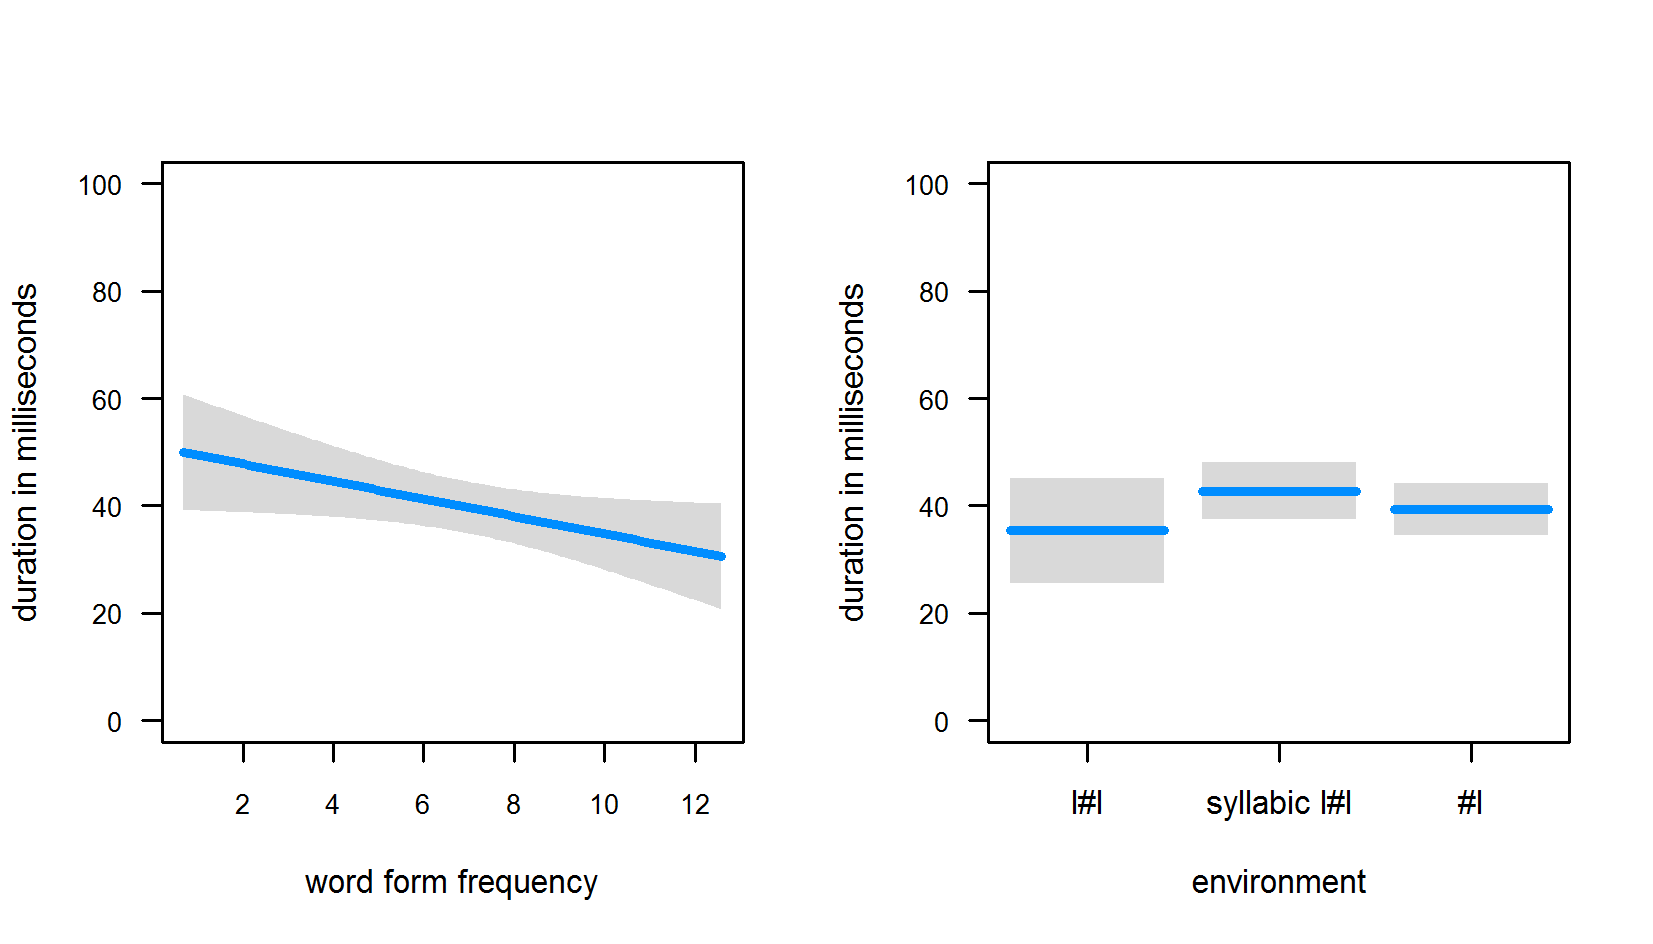
\includegraphics[scale=.8] {images/Corpus/lyModelTransitionTypeAndFreq.png}
	\caption{Effects of word form frequency  and environment on consonant duration in \suffix{ly}-data set}
	\label{fig:corpus main effects  ly}
\end{figure*}




To see which are the most predictive variables for consonant duration in the \is{-ly}\suffix{ly}-data set, I conducted a \isi{multi-model inferencing} analysis. As for the other data sets, the analyses did not include the variable \textsc{LSAScore} because of the low number of observations which were coded for \textsc{LSAScore}. The analysis revealed that \textsc{LocalSpeechRate} is the most important variable (importance value: $1$). With an importance value of $0.99$ the variable \textsc{PrecedingSegment} is the second most important value. It is followed by the two \isi{frequency} variables log\textsc{RelativeFrequen-cy} (importance value: $0.67$) and log\textsc{WordFormFrequency} (importance value: $0.64$). With importance values of $0.32$ (\textsc{Environment}) and $0.26$ (\textsc{BaseFinalStress}), the other variables are far less important for predicting consonant duration with \is{-ly}\suffix{ly}.


\subsubsection{Relative duration}

To test whether the affix \is{-ly}\suffix{ly} geminates in terms of \isi{relative duration}, it was necessary to create a subset. This subset only includes words which feature a vowel at the end of their base, i.e. words in which the suffix is preceded by a vowel. This was necessary because \isi{relative duration} (as a measure of \isi{gemination}) is calculated by dividing consonant duration by preceding vowel duration. Since the complete data set includes words which are preceded by a consonant, the creation of the subset was necessary.
However, the subset only includes 48 tokens, i.e. it is very small. Furthermore, in this data set only the difference in duration between two of the pertinent environments can be tested, i.e. \texttt{l\#l} and \texttt{\#l}. The items featuring a \is{syllabicity}syllabic double (\texttt{\is{syllabicity}syllabic l\#l}) had to be excluded since they are always preceded by a consonant. 

The small size of the data set restricted the number of noise variables included in the model, i.e. to avoid \isi{overfitting}, only few variables were tested in the model. I chose to only include those noise variables which showed a significant effect in the \isi{absolute duration} model, i.e. \textsc{LocalSpeechRate} and log\textsc{WordFormFrequen-cy}. The variable \textsc{PrecedingSegment} was not included because all of the preceding segments in the data set were vowels. The model was then fitted according to the same procedure as the \isi{absolute duration} model. The residuals were normally distributed, and thus no transformation of the dependent variable was necessary and no items had to be excluded.

The final model reached an adjusted R-squared of $0.184$, i.e. it explains 18\% of the variance in the data. As with the other affixes, the \isi{relative duration} model is thus worse than the \isi{absolute duration} model. Only one variable remained in the final model, log\textsc{WordFormFrequency}. The higher the \isi{frequency}, the shorter the \isi{relative duration} of the consonant ($estimate= -0.129$, $t$-$value=-3.533, p=0.001$). In contrast to the \isi{absolute duration} model, \textsc{LocalSpeechRate} did not reach significance. Crucially, \textsc{Environment} did not reach significance. Doubles are not longer than singletons in terms of \isi{relative duration}, i.e. they degeminate.
Because of the low number of observations in the subset, no \isi{multi-model inferencing} analysis was conducted.

\subsubsection{Summary}
Two models predicting consonant duration with \is{-ly}\suffix{ly} were fitted, one predicting \is{absolute duration}absolute consonant duration and one predicting relative consonant duration. The usefulness of the \isi{relative duration} model is, however,  restricted by the small number of observations which were taken into account in this model. In both models only noise variables showed significant effects. 
In the \isi{absolute duration} model, the expected effects of \textsc{LocalSpeechRate}, \textsc{PrecedingSegment} and log\textsc{WordFormFrequency} were found. In the \isi{relative duration} model only log\textsc{WordFormFrequency} had a significant effect on consonant duration.
Crucially, the variable \textsc{Environment} did not have a significant effect on consonant duration, neither in absolute nor in \isi{relative duration}. Multi-model inferencing also showed that this variable is not an important predictor for consonant duration with \is{-ly}\suffix{ly}. Thus, the suffix \is{-ly}\suffix{ly} clearly degeminates.
The \is{decomposability measure}decomposability variables did not prove to be significant in either model.




\subsection{Summary} \label{Summary Corpus Study}

The first durational analyses looked at the distribution of duration across environments to get a first impression of whether the affixes under investigation geminate, and if so, whether \isi{gemination} is a gradient or a categorical phenomenon. 
For the prefixes, the analyses revealed that the distribution of duration in the data sets is bimodal, with the double consonants being significantly longer than the singletons. This indicates that the prefixes geminate, and that \isi{gemination} is categorical. The distribution for \is{-ly}\suffix{ly} is not bimodal, and doubles are not longer than singletons. This suggests \isi{degemination} with \is{-ly}\suffix{ly}. The impression that the prefixes geminate and that the suffix degeminates was validated in the linear models.


For all data sets at least two linear models were fitted, one predicting \is{absolute duration}absolute consonant duration and one predicting relative consonant duration. 
In general, both models reveal very similar results, i.e. for the most part the same variables are significant in both models. However, the relative models feature fewer variables than the absolute models.  Importantly, the effects of the variables of interest do not differ between the models, i.e. the same variables of interest are significant in both models. The \isi{relative duration} models only feature less noise variables. 
The variable \textsc{Environment} shows stronger effects in absolute than in \isi{relative duration}. 
Furthermore, for all affixes, the \isi{absolute duration} models explain more of the variance in the data than the \isi{relative duration} models. 
The results thus suggest that \is{absolute duration}absolute consonant duration is a better measure of \isi{gemination} than relative consonant duration. In other words, \is{morphological gemination}{gemination} in English is not expressed by a particular consonant-vowel ratio but by \is{absolute duration}absolute consonant duration. 
In what follows I will therefore concentrate on \is{absolute duration}absolute consonant duration.

\begin{table*}
	\caption{Overview of significant variables in absolute duration models}
	\label{tbl: Overview of results in the corpus study}
	
	%	
	
		%			\resizebox{\textwidth}{!}{%		
		\begin{tabular} {lccccc}
			
			\lsptoprule
			\textbf{Variable} & \textbf{un-} & \textbf{im-} &\textbf{un-} &\textbf{dis-}& \textbf{-ly}\\
			& & &\& \textbf{im-}  && \\
			\midrule			
			\textsc{Environment}& \checkmark & \checkmark  & \checkmark & \checkmark & n.s. \\ 
			\textsc{Affix }&- &\checkmark  & \checkmark  &- & -\\ 
			
			\textsc{SemanticTransparency}&-& n.s. &  - & (\checkmark) & - \\
			\textsc{LocalSpeechRate}&\checkmark & \checkmark & \checkmark  &\checkmark  & \checkmark \\			
			\textsc{BaseInitialStress}&n.s.& \checkmark & \checkmark & \checkmark &-\\
			\textsc{Voicing}& - & - & - &\checkmark  & - \\
			\textsc{PrecedingSegment}&-& -& - & - &\checkmark\\
			log\textsc{WordFormFrequency}&n.s.& n.s.& n.s. & n.s.&\checkmark\\
			
			\midrule\\
			
			\multicolumn{6}{l}{\small \checkmark \hspace*{0.2cm}: significant in at least one of the \isi{absolute duration} models} \\			
			\multicolumn{6}{l}{\small n.s. : not significant in any of the \isi{absolute duration} models} \\			
			\multicolumn{6}{l}{\small - \hspace*{0.45cm}: not included in the \isi{absolute duration} models} \\	\\
			\lspbottomrule		
			
		\end{tabular}
		%	}
	
	
	
	
\end{table*}


\tabref{tbl: Overview of results in the corpus study} shows an overview of the variables which show significant effects on \is{absolute duration}absolute consonant duration in the subsets. Only variables which are significant in at least one of the \isi{absolute duration} models are listed. For \is{dis-}\prefix{dis}, the table indicates all variables which are significant in at least one of the two \isi{absolute duration} models fitted, i.e. the model including all \is{dis-}\prefix{dis}prefixed items and the model including only voiceless items.







Let us first discuss the noise variables. The variable \textsc{LocalSpeechRate} shows the expected effect in all models.  The higher the \isi{speech rate}, the shorter the duration of the consonant. 
For \is{dis-}\prefix{dis}, the variable \textsc{Voicing} is significant in the complete model. As expected, voiced items are shorter than voiceless items. The variable is irrelevant for all other models.

\textsc{BaseInitialStress} affects consonant duration in the \is{in-}\prefix{in}model and in the \is{un-}\prefix{un} and \is{in-}\prefix{in} model. Before unstressed base-initial syllables the consonant is shorter than before \is{stress}stressed base-initial syllables. 
In the \is{dis-}\prefix{dis}models, \textsc{BaseInitialStress} forms interactions with \textsc{Environment} and \textsc{SemanticTransparency}. As discussed thoroughly in \sectref{corpus results dis}, these interactions were caused by only a few items and their interpretation is therefore unclear. Either only \is{dis-}\prefix{dis}prefixed items with a double consonant are affected by \textsc{BaseInitialStress}, or only semantically opaque items are affected by \isi{stress}.

 \textsc{BaseInitialStress} does not affect consonant duration with \is{un-}\prefix{un}. The reason for the absence of the effect might be due to the distribution of \textsc{BaseInitialStress} across \is{un-}\prefix{un}prefixed words. Most \is{un-}\prefix{un}words feature a \is{stress}stressed base-initial syllable. This includes all items with a double consonant. This lack of variation in \isi{stress} might have caused the absence of the effect with \is{un-}\prefix{un}. It is also possible that other factors, such as \is{stress}prefixal stress, might have interfered with the effect of \textsc{BaseInitialStress}. As discussed in Chapter \ref{affixes}, the \isi{stress} status of \is{un-}\prefix{un} is yet unclear. Further research on \is{stress}prefixal stress is necessary to explore the relation of \isi{stress} and prefixal consonant duration further. This is, however, beyond the scope of this study.

For the suffix \is{-ly}\suffix{ly}, the two variables \textsc{PrecedingSegment} and log\textsc{WordFormFre-quency} show the expected effects. The consonant is shorter after a consonant than after a vowel, and more frequent words display shorter consonant durations than less frequent words. While \textsc{PrecedingSegment} was only coded for \is{-ly}\suffix{ly}, the variable log\textsc{WordFormFrequency} was included in all models. Only for \is{-ly}\suffix{ly} it affected consonant duration. There are various possible explanations for this. 
One possibility is that \isi{word form frequency} only affects consonant duration in suffixes but not in prefixes. Another possibility is that, while the effect exists for all affixes, it only reaches significance in the \is{-ly}\suffix{ly}-model. There are two arguments for this explanation.
 First, the \is{-ly}\suffix{ly}-model is the worst of all models, i.e. it explains the least variance. It is therefore easier for weaker effects to reach significance. 
 Second, out of all data sets the \is{-ly}\suffix{ly}-data set features the highest number of different types. Different types have different \is{frequency}frequencies, i.e. the distribution of log\textsc{WordFormFrequency} shows more variation in the \is{-ly}\suffix{ly}-data set than in the other data sets. As already discussed above, the lack of variation in the distribution of a variable might make it impossible to find effects. In other words, there might not be enough variation in log\textsc{WordFormFrequency} in the prefixal data sets to find effects.


Let us now turn to the variables of interest. Out of the five \is{decomposability measure}decomposability measures only \textsc{SemanticTransparency} showed an effect on consonant duration. This effect was, however, only found in one model, i.e. the model predicting \is{absolute duration}absolute consonant duration with voiceless \is{dis-}\prefix{dis}.  Furthermore, the effect was only found in interaction with the variable \textsc{BaseInitialStress}. Since the interaction was caused by only a few items in the data set, its validity is yet unclear. 
In none of the other models \isi{decomposability} directly played a role. 
However, in two of the models \isi{decomposability} indirectly influenced duration. As discussed in \sectref{corpus dec}, the five affixes differ in their overall \isi{segmentability}. This difference is mirrored in consonant duration in the \is{in-}\prefix{in} and in the \is{un-}\prefix{un} and \is{in-}\prefix{in} model. In these models, the variable \textsc{Affix} significantly affects consonant duration. The affix \is{un-}\prefix{un} features the longest nasal, \is{negative in-}negative \prefix{in} features a significantly shorter nasal, and \is{locative in-}locative \prefix{in} has the shortest nasal out of the three. This decline in duration resembles the decline in \isi{segmentability} of the affixes. The prefix \is{un-}\prefix{un} is the most segmentable affix of the three, followed by \is{negative in-}negative \prefix{in}, followed by \is{locative in-}locative \prefix{in}. Thus, while word-specific \is{decomposability measure}decomposability measures did not affect consonant duration in the models, \isi{decomposability} influenced consonant duration in terms of the overall \isi{segmentability} of the affix.


The variable \textsc{Environment} significantly affected consonant duration in all prefixal models. For \is{-ly}\suffix{ly}, there was no significant difference in duration between the three tested environments.
\tabref{tbl: Overview of environment in the corpus study} summarizes the predicted durations for all environments for all affixes. The table also shows the significant differences in predicted durations between doubles and singletons for the prefixes, as well as singleton-geminate ratios.
The conditions of the predicted values are the same as in the partial effects plots, i.e. numerical variables are held constant at their median and categorical variables are held constant at the most common category. For \is{dis-}\prefix{dis}, two predicted values are shown, one for the complete data set (for words with a \is{stress}stressed base-initial syllable), and one for the voiceless data set.







\begin{table}
	\caption{Overview of predicted durations in the corpus studies}
	\label{tbl: Overview of environment in the corpus study}
	
	
					\resizebox{\textwidth}{!}{%		
		\begin{tabular} {lcccc}
		\lsptoprule
			
			\multicolumn{5}{l}{\textbf{Predicted durations}}\\
					\\
			&  \multicolumn{2}{c}{Phonological Doubles } &  \multicolumn{2}{c}{Phonological Singletons } \\
		%	&in Complex Words & in Complex Words &in Complex Words\\
			& 					(non-\is{syllabicity}syllabic)						&(\is{syllabicity}syllabic)			& (consonant-adjacent) &(vowel-adjacent)\\
			%	&Double -Singleton & Double -Singleton &\\
			\midrule			
			\isi{un-}& 90~ms &NA& 63~ms   & 43~ms\\ 
			\isi{im-}& 95~ms&NA& 68~ms & NA  \\ 

			\isi{dis-}\textsuperscript{1}   & 136~ms&NA& 98~ms& 113~ms\\
			\isi{dis-}\textsuperscript{2}&142~ms&NA& 98~ms &  97~ms\\

			%& Phonological Doubles & Phonological Doubles &Phonological Singleton \\
				%		&in Complex Words & in Complex Words &in Complex Words\\
			%&(non-\is{syllabicity}syllabic)&(\is{syllabicity}syllabic) &\\

			\isi{-ly}&35~ms& 43~ms &   \multicolumn{2}{c}{39~ms}\\
			
			
			\midrule

			\\
			
						\\
						\multicolumn{3}{l}{\textbf{Durational difference}}&\multicolumn{2}{l}{\textbf{Singleton-Geminate Ratio}}\\
						\\			
						&Double-Singleton  &Double-Singleton  &Singleton-Double  &Singleton-Double  \\
						&(consonant-adjacent) &(vowel-adjacent)& (consonant-adjacent) &(vowel-adjacent)\\


			%	&Double -Singleton & Double -Singleton &\\
			\midrule			
			\isi{un-}& 27~ms & 47~ms   & 1:1.4 & 1:2.1\\ 
			\isi{im-}&27~ms &NA  & 1:1.4 & NA\\ 
			\isi{dis-}\textsuperscript{1}  &38~ms& 23~ms & 1:1.4& 1:1.2 \\
			\isi{dis-}\textsuperscript{2} &44~ms& 45~ms &1:1.5& 1:1.5\\
			
			%\isi{-ly}&- & - & &  \\			
			
			\midrule
			\\

			\multicolumn{5}{l}{\textsuperscript{1} \footnotesize{\is{stress}stressed base-initial syllable}}\\
			\multicolumn{5}{l}{\textsuperscript{2} \footnotesize{voiceless}}\\
			\lspbottomrule

		\end{tabular}
	}
	
	

	
\end{table}


For \is{un-}\prefix{un}, \is{in-}\prefix{in} and \is{dis-}\prefix{dis}, double consonants are significantly longer than corresponding singletons. The only exception might be the double consonant in the word \textit{dissolution}. In the \is{dis-}\prefix{dis}model with all words, i.e. voiced and voiceless \is{dis-}\prefix{dis}prefixed words, a significant interaction between \textsc{Environment} and \textsc{BaseInitialStress} was found. Double consonant items with an unstressed base-initial syllable, i.e. words of the type \textit{dissolution}, degeminated. However, it is yet unclear whether this effect is universal, i.e. whether it applies to all \is{dis-}\prefix{dis}prefixed words with a double consonant and an unstressed base-initial syllable,  or whether the effect is caused by other factors, such as the word's opacity or type-specific effects. In Chapter \ref{Experimental Studies}, we will turn back to this question after considering the results of the experimental study.

The durational differences between doubles and singletons range from 23~ms to 47~ms.  The  \is{singleton-geminate ratio}{singleton-double ratio} for singletons followed by a consonant is comparable across all prefixes. The ratio is 1:1.4 for \is{un-}\prefix{un}, \is{in-}\prefix{in}, and \is{dis-}\prefix{dis} (in the complete data set). For voiceless \is{dis-}\prefix{dis} the ratio is 1:1.5.
For singletons followed by a vowel, the absolute durational difference between doubles and singletons is practically the same for \is{un-}\prefix{un} and voiceless \is{dis-}\prefix{dis} (47~ms and 45~ms), but smaller for voiced and voiceless \is{dis-}\prefix{dis} (23~ms). The absolute durational differences for \is{dis-}\prefix{dis} and \is{un-}\prefix{un} suggest that both prefixes geminate to the same degree. However, the double-singleton ratios suggest the opposite. The ratio for \is{un-}\prefix{un} is much bigger than the ones for \is{dis-}\prefix{dis}. This indicates that \is{un-}\prefix{un} geminates to a higher degree than \is{dis-}\prefix{dis}.


In addition to the difference between doubles and singletons, a significant difference between the two singleton levels was found for \is{un-}\prefix{un}. Consonants followed by a vowel are significantly shorter than consonants followed by a consonant. This difference between the two singleton environments was not found for \is{dis-}\prefix{dis}. For \is{-ly}\suffix{ly} the variable \textsc{Environment} never reached significance, i.e. singletons, non-\is{syllabicity}syllabic doubles and \is{syllabicity}syllabic doubles are predicted to be of the same duration.

 A comparison of the singleton-double ratios found in this study with the ones in former studies is limited. Only two studies have investigated \isi{gemination} with the investigated affixes, i.e. \cite{Kaye.2005} and \cite{Oh.2012}. Out of the two, only \cite{Oh.2012} provide enough data for a sensible comparison. The comparison with \citeauthor{Oh.2012}'s study is, however, also restricted as they only investigated the prefixes \is{un-}\prefix{un} and \is{in-}\prefix{in} under experimental condition. Furthermore, consonant duration was only analyzed in intervocalic position, which forbids a straightforward comparison. 
 
 For \is{un-}\prefix{un}, \cite{Oh.2012} find a ratio of 1:1.6 in \isi{normal speech}, and a ratio of 1:2.0 in \isi{careful speech}. For \is{in-}\prefix{in}, they find a ratio of 1:1.3 in normal and a ratio of 1:1.2 in \isi{careful speech}. 
 As \isi{normal speech} can be assumed to be more similar to \isi{conversational speech} than \isi{careful speech}, the singleton-geminate ratios of the present corpus study should be compared to the ones for \isi{normal speech}. 
 For both \is{un-}\prefix{un} and \is{in-}\prefix{in}, the comparison shows that the ratios found in the present study are bigger than the ones in \cite{Oh.2012}. 
  One reason for this difference might be the different conditions under which the items were recorded, i.e. natural conversation vs. \is{experimental speech}experimental reading. The experimental study on \isi{gemination} will shed more light on this issue.

To summarize, the prefixes \is{un-}\prefix{un}, \is{in-}\prefix{in} and \is{dis-}\prefix{dis} geminate. The suffix \is{-ly}\suffix{ly} degeminates. No word-specific effect of \isi{decomposability} was found, but the \isi{segmentability} of the affix affected consonant duration in the expected way. Less segmentable affixes have shorter consonant durations. The effect of affix is independent of \isi{gemination}, i.e. all prefixes geminate. The comparison of singleton-geminate ratios indicates, however, that the prefix \is{un-}\prefix{un} geminates to a higher degree than the prefix \is{dis-}\prefix{dis}.

\subsection{Discussion}


The corpus study shows that \isi{gemination} is affix-specific and categorical. While the prefixes geminate, the suffix \is{-ly}\suffix{ly} degeminates. 
This result falsifies common assumptions about the \isi{gemination} pattern of English affixes as found in the literature (cf. \sectref{assumption gem English}). 
With regard to the theoretical approaches discussed in Chapter \ref{Theory}, the result falsifies word-specific approaches, and supports approaches which predict categorical \isi{gemination} that depends on the affix. However, as thoroughly discussed in Chapter \ref{Theory}, there are important differences in the predictions of the affix-specific approaches. In other words, the affix-specific approaches make different predictions about which affixes should geminate and which should degeminate. Therefore, it is necessary to look at the predictions of each of these approaches individually, and to compare them to the \isi{gemination} pattern found in the study.

Let us first look at the formal linguistic approaches discussed. Even though all of them are categorical in nature and predict \isi{gemination} to be affix-specific, none of them is supported by the data. The fact that the \is{level 2 affix}{level 2} affix \is{-ly}\suffix{ly} degeminates, while the \is{level 1 affix}{level 1} affixes \is{dis-}\prefix{dis} and \is{in-}\prefix{in} geminate, falsifies the predictions made by \is{stratal approach}{stratal approaches}. That \is{in-}\prefix{in} and \is{dis-}\prefix{dis} geminate furthermore falsifies the predictions made by the Prosodic Word Approach according to which one should find variation in their \isi{gemination} pattern. 

With regard to the psycholinguistic approaches discussed, only the two affix-specific approaches can be supported by data, i.e. the affix-specific Segmentability Approach and the affix-specific Morphological Informativeness Approach. 
These two approaches are based on the two lexical \isi{segmentability} hierarchies introduced in Chapter \ref{affixes} (see \figref{fig:Segmentability hierarchies of  affixes repetition 2} for the two hierarchies). While the affix-specific Morphological Informativeness Approach predicts \isi{gemination} to pattern according to the Semantic Segmentability Hierarchy, the affix-specific Segmentability Approach does not specify according to which of the two \isi{segmentability} hierarchies \isi{gemination} should pattern. In other words, while the affix-specific Morphological Informativeness Approach is only supported if \isi{gemination} patterns according to the Semantic Segmentability Hierarchy, the affix-specific Segmentability Approach is also supported if \isi{gemination} patterns according to the Non-Semantic Segmentability Hierarchy. 


The corpus study reveals that \isi{gemination}, at least partly, patterns according to the Semantic Segmentability Hierarchy (\prefix{un} > \{\prefix{dis}, \prefix{in}\textsubscript{\textsc{Neg}}\} >  \prefix{in}\textsubscript{\textsc{Loc}} > \suffix{ly}). 
The least segmentable and least informative affix \is{-ly}\suffix{ly} degeminates, while all other affixes geminate. The most segmentable affix \is{un-}\prefix{un} displays a higher singleton-geminate ratio than the less segmentable affix \is{dis-}\prefix{dis}, i.e. \is{un-}\prefix{un} geminates to a higher degree than \is{dis-}\prefix{dis}. However, the data does not suggest a difference in \isi{degree of gemination} between \is{in-}\prefix{in} and \is{un-}\prefix{un}, or between the two \is{in-}\prefix{in}prefixes.
 It is not yet clear whether such differences are non-existent, or whether, due to methodological reasons, they were not detected in the data set. 
  In contrast to \is{un-}\prefix{un} and \is{dis-}\prefix{dis}, only two environments were investigated for \is{in-}\prefix{in}, i.e. \texttt{m\#mV} and \texttt{m\#C}. The difference in \isi{degree of gemination} between \is{un-}\prefix{un} and \is{dis-}\prefix{dis} was only detected by comparing the singleton-geminate ratio of doubles and singletons followed by a vowel, a ratio which could not be calculated for \is{in-}\prefix{in}. Thus, there might be differences between the \isi{degree of gemination} of \is{un-}\prefix{un} and \is{in-}\prefix{in} which could not be detected in this study.
Furthermore, the model directly comparing \is{un-}\prefix{un}, \is{negative in-}negative \prefix{in} and \is{locative in-}locative \prefix{in} indicates that the difference in \isi{segmentability} and \isi{informativeness} between the three prefixes affects their \isi{phonetic realization} in the predicted direction. The model revealed that the nasal in \is{un-}\prefix{un} is longer than the one in \is{negative in-}negative \prefix{in}, which in turn is longer than the one in \is{locative in-}locative \prefix{in}. Thus, while there is no difference in the \isi{degree of gemination} between the three prefixes, there is a general difference in  their nasal duration.
 
 To conclude, the corpus study provides evidence that the \isi{phonetic realization} of the investigated affixes, including the realization of morphological geminates, patterns according to the Semantic Segmentability Hierarchy. The pattern of \isi{gemination} is, however, not yet clear and further evidence is needed. 
 Up until now, the affix-specific Segmentability Approach (which is based on the Semantic Segmentability Hierarchy) and the affix-specific Morphological Informativeness Approach are the only two approaches not falsified by the data, i.e. they are the two approaches which, based on the corpus study, explain \is{morphological gemination}{gemination} in English affixation the best.


Apart from evidence for the \isi{gemination} pattern of English affixes, the corpus study also revealed important insights with regard to the \isi{phonetic realization} of alleged \is{homophone}homophones. The data shows that there is a durational difference between the two \is{in-}\prefix{in}prefixes. This has important implications for current \is{speech production model}{models of speech production}. Models which do not allow for morphological information to be visible on the phonetic level need to be revised with regard to this aspect.



While the corpus study has revealed some important insights for theories of the \isi{morpho-phonological interface}, a number of questions remain  unanswered. Due to the limited number of types and tokens, some effects could not be investigated properly in the study, i.e the distribution of the data did not allow for valid investigations of some factors. Furthermore, one must complement the corpus data by experimental data, which is more controlled and therefore less prone to distorting effects.
   
% \chapter{Experimental study} \label{Experimental Studies}


The experimental study was conducted to replicate and complement the results of the corpus study. In contrast to the corpus study, the experimental study did not investigate natural, \isi{conversational speech} but \isi{read speech}. As thoroughly discussed in Chapter \ref{General Method}, this has the advantage of including a great number of types and tokens and investigating durational properties of words under controlled conditions.

 The data was collected in two experiments carried out in October 2015 and October 2016 at the University of Cambridge's Phonetic Laboratory. While in the first experiment the \is{un-}\prefix{un} and \is{in-}\prefix{in}data was collected, the second experiment was conducted to record the \is{dis-}\prefix{dis} and \is{-ly}\suffix{ly}-data. 
  The set-up of both experiments was identical. The experiments consisted of two parts, a reading task and a decomposability rating. 
 Both experimental tasks will be described in detail in the first section of this chapter.
 The data was analyzed with regard to two aspects, \isi{decomposability} and duration. First, I will describe the \isi{decomposability} analysis.  Then, I will lay out the durational analyses and their results. At the end of the chapter, I will summarize the results. A thorough discussion of the results and their theoretical implications will be conducted alongside with the results from the corpus study in Chapter \ref{Conclusion}.



\section{Methodology}


\subsection{Stimuli} \label{stimuli experiment}

% investigated strutuctues
 Five different structures were investigated in the experimental studies. The structures and their environments are shown in \tabref{tbl:overview structures environment experiment repetition}. For each of the investigated affixes, the included environments and examples are listed (see \sectref{experiment data composition} for a detailed description of the investigated structures and environments). In contrast to the corpus study, the experimental study did not only investigate the allomorph \is{im-}/ɪm/  for the prefix \is{in-}\prefix{in}, but also /ɪn/. Note that no distinction between locative and \is{negative in-}negative \prefix{in} is made in the table but that this distinction was taken into consideration when selecting the experimental items, as well as when analyzing the data.



\begin{table*}
	
	\caption{Overview of the investigated structures in the experimental study}
	\label{tbl:overview structures environment experiment repetition}
					
	
	\resizebox{\textwidth}{!}{%
		\begin{tabular}{ccccc} 
		\lsptoprule
		
			& \begin{tabular}[c]{@{}c@{}} Phonological double\\ in complex word\end{tabular}                           &  \begin{tabular}[c]{@{}c@{}}Singleton\\ in complex word\end{tabular}                                                   & \begin{tabular}[c]{@{}c@{}}Singleton \\ in base\end{tabular}               &
			\begin{tabular}[c]{@{}c@{}}Orthographic double\\ in simplex word\end{tabular} \\
			\midrule
			%\\
			
			\{\isi{un-}\}  & 
			{\begin{tabular}[c]{@{}c@{}}\color{lsMidBlue} \textit{unnatural}\\ (n\#nV)\end{tabular}}         & {\begin{tabular}[c]{@{}c@{}}\color{lsMidBlue} \textit{uneven \phantom{space} untold} \\ (n\#V)\phantom{space }(n\#C)\end{tabular}}                               & {\begin{tabular}[c]{@{}c@{}}\color{lsMidBlue} \textit{natural}\\ (\#nV)\end{tabular}  } &
			NA                                                                            
			\\
			\\
			
			\{\isi{in-}\}  & 
			{\begin{tabular}[c]{@{}c@{}}\color{lsMidBlue} \textit{immortal}\\ (m\#mV)\\ \color{lsMidBlue} \textit{innumerous}\\ (n\#nV)\end{tabular}} & 
			 {\begin{tabular}[c]{@{}c@{}}\phantom{spa} NA \phantom{spa} \color{lsMidBlue} \textit{impossible}\\ \phantom{more space } (m\#C)\\ \color{lsMidBlue} \textit{inefficient \phantom{sp}   intolerant}\\ (n\#V)\phantom{space } (n\#C)\end{tabular}} & {\begin{tabular}[c]{@{}c@{}}\color{lsMidBlue} \textit{mortal}\\ (\#mV)\\ \color{lsMidBlue} \textit{numerous}\\ (\#nV)\end{tabular}} &
			 NA                                                                            \\
			\\
			
			\{\isi{dis-}\} & 
			{\begin{tabular}[c]{@{}c@{}}\color{lsMidBlue} \textit{dissatisfy}\\ (s\#sV)\end{tabular}}                      &
			
			{\begin{tabular}[c]{@{}c@{}}\color{lsMidBlue} \textit{disarm \phantom{space} } \color{black} NA\\ (s\#V)\phantom{space} \phantom{s\#V} \end{tabular}}                   & {\begin{tabular}[c]{@{}c@{}}\color{lsMidBlue} \textit{satisfy}\\ (\#sV)\end{tabular}}        &
			{\begin{tabular}[c]{@{}c@{}}\color{lsMidBlue} \textit{dissertation}\\ (sV)\end{tabular}}                     \\
			\\
			
			\{\isi{-ly}\}  & 
			{\begin{tabular}[c]{@{}c@{}}\color{lsMidBlue} \textit{really}\\ (Vl\#l)\end{tabular}}                           & 
			{\begin{tabular}[c]{@{}c@{}}\color{lsMidBlue} \textit{truly \phantom{spaceee}} \color{black} NA\\ (V\#l)\phantom{space }\phantom{V\#C}\end{tabular}}                 & {\begin{tabular}[c]{@{}c@{}}\color{lsMidBlue} \textit{real}\\ (Vl\#)\end{tabular}}      &
			{\begin{tabular}[c]{@{}c@{}}\color{lsMidBlue} \textit{belly}\\ (Vl)\end{tabular}}                                
			
			\\	\lspbottomrule
		\end{tabular}%
		
	}
	

\end{table*}


The experimental stimuli were selected from a word list that features all words with the desired structures attested in \is{Corpus of Contemporary American English (COCA)} {COCA} (\citealt{Davies.20082014}). This list was generated using the speech corpus management system Coquery (\citealt{Kunter.2016}). The selection of stimuli was then guided by several criteria. 
The first criterion was that only types which are attested in the \textit{OED} (\citealt{OED.2013}) were considered to serve as stimuli in the experiments. 
The second criterion concerns morphological structure. All complex stimuli in the experiments had to feature different roots.\footnote{As in the corpus study, morphological structure was coded by using the criteria described in \sectref{theory:in}.} For example, since the two derivatives \textit{unnatural} and \textit{unnaturally} feature the same root, i.e. \{nature\}, only one of them was included in the study. Complex words with fewer morphemes were preferred over complex words with more morphemes, e.g. the word \textit{unnatural} was preferred over the word \textit{unnaturally}. 
 The third criterion concerns \isi{word form frequency}. For each environment, types of different \is{frequency}frequencies were selected, i.e. the same number of types with low, mid and high \isi{frequency} were selected. A low \isi{frequency} word was defined to have a \isi{frequency} lower than 10, a mid \isi{frequency} word was defined to have a \isi{frequency} between 10 and 100, and a high \isi{frequency} word was defined to have a \isi{frequency} higher than 100. Frequency measures were taken from \is{Corpus of Contemporary American English (COCA)} {COCA} (\citealt{Davies.20082014}).
  The fourth criterion concerns prosodic structure. When possible, the number of syllables and the \isi{stress} pattern of the stimuli was kept similar across the environments of each affix. In other words, the distribution of \isi{stress} and syllable number in a particular environment should not be unique to that environment. To test whether the prosodic structure of the stimuli differed significantly between the environments of a particular affix, Wilcoxon Signed-Rank tests (see, for example, \citealt{Crawley.2012}, chapter 5) were applied. In case prosodic features differed significantly, additional stimuli were added until there was no significant difference between environments.
 
 %affix-specific criteria
 In addition to the four criteria just mentioned, which applied to all stimuli, some criteria only applied to words with specific affixes. 
 For \is{dis-}\prefix{dis}, only words featuring voiceless /s/ were included in the study. 
  For \is{in-}\prefix{in} and \is{dis-}\prefix{dis}, when possible, the same number of \is{semantic transparency}semantically transparent and opaque words was included for each environment. Since \is{un-}\prefix{un} and \is{-ly}\suffix{ly}-affixed words do not show variation in \isi{semantic transparency} (see \sectref{The decomposability of the four affixes: a comparison} for discussion), this criterion was irrelevant for these data sets.
 Furthermore, when possible, the same number of derivatives with negative and \is{locative in-}locative \prefix{in} was included for each of the \is{in-}\prefix{in}environments. 
 
 

 %application of criteria
The application of the selection criteria led to different numbers of included stimuli for each affix and each environment. 
There are two reasons for these differences. The first reason is that for some environments only few types are attested, i.e. the number of included stimuli is restricted by the number of existing types. The second reason is methodological in nature. 
In some environments 
certain features, for example, base-initial \isi{stress} and high \isi{word form frequency}, tend to appear together. This raises the problem that certain effects cannot be tested independently from each other. To alleviate the problem, i.e. to ensure the independence of effects, it was sometimes necessary to add more stimuli with a certain combination of features to an environment. As a result, for some environments more stimuli were included than for others. 
In the following, I will discuss the stimuli selection for each affix. In these discussions, I will also point out for which environments the selection criteria were not, or only partially, met.\footnote{A list of all experimental stimuli can be found in \hyperref[Appendix E: Stimuli of Experimental Study]{Appendix E}.} 


\subsubsection{un-}

\tabref{tbl:distribution of un types in experiment} shows the distribution of  stimuli in the \is{un-}\prefix{un}data set across environments. 
%Doubles for the prefixes
22  \is{un-}\prefix{un}prefixed stimuli with a phonological double ({n\#nV}) were included. These 22 stimuli represent all \is{un-}\prefix{un}prefixed types with a phonological double and different roots attested in \is{Corpus of Contemporary American English (COCA)} {COCA} (\citealt{Davies.20082014}) and the \textit{OED} (\citealt{OED.2013}). 
Due to the small number of available types, only the first two selection criteria (attestation in the \textit{OED} (\citealt{OED.2013}) and different roots) were taken into account when selecting these stimuli. Considering the other selection criteria would have resulted in a fatal decrease of available stimuli. 



The number of stimuli with singleton environments in complex words (n\#C and n\#V) roughly matches the number of stimuli with a double consonant. 21 types with a  singleton followed by a consonant ({n\#C}), and 26 types with a singleton followed by a vowel ({n\#V}) were included. 
Of the 21 \is{un-}\prefix{un}prefixed words with a following consonant, seven were of high, seven of mid, and seven were of low \isi{frequency}.
For the following-vowel words, eight items were of low \isi{frequency}, eight of mid \isi{frequency} and 10 of high \isi{frequency}. The reason for including more stimuli of high \isi{frequency} was due to the distribution of prosodic structure across the environments. To make the prosodic structure of \is{un-}\prefix{un}prefixed words with a singleton comparable to the one of \is{un-}\prefix{un}prefixed words with a double consonant, some additional words with a specific prosodic structure needed to be added to the data set. These words were of high \isi{frequency}.




%Base words
The selection of the base words ({\#nV}) was determined by the selection of words with a phonological double, i.e.  for each word with a phonological double the pertinent base word was included in the experiment. Two base words were not included in the study due to a mistake in the experimental set-up. 




%Overview table

\begin{table}
	\caption{Distribution of  {un}-types in experimental study}
	\label{tbl:distribution of un types in experiment}

	
		\begin{tabular} {llr}
\lsptoprule
			Environment & Example & Number of  Types\\

			\midrule
			n\#nV&\color{lsMidBlue}\textit{unnatural} & 22\\ 
			n\#C&\color{lsMidBlue}\textit{untold} & 21\\ 
			n\#V&\color{lsMidBlue}\textit{uneven} & 26 \\
			\#nV&\color{lsMidBlue}\textit{natural} & 20 \\ 
			\midrule
			Total&  & 89 \\ 
			\lspbottomrule                                                                                
		\end{tabular}
		

	
\end{table}



\subsubsection{in-}

\tabref{tbl:distribution of in types in experiment} shows the distribution of  stimuli in the /ɪn/-data set across environments. 
Four stimuli with a phonological double ({n\#nV}) were included. As with \is{un-}\prefix{un}, these four stimuli represent all /ɪn/-prefixed types with a phonological double and different roots attested in \is{Corpus of Contemporary American English (COCA)} {COCA} (\citealt{Davies.20082014}) and the \textit{OED} (\citealt{OED.2013}). Only the first two selection criteria (attestation in the \textit{OED} (\citealt{OED.2013}) and different roots) were taken into account when selecting these stimuli. 



Only 19 /ɪn/-prefixed types with a following /t/ ({n\#C}) were attested  in \is{Corpus of Contemporary American English (COCA)} {COCA} (\citealt{Davies.20082014}) and the \textit{OED} (\citealt{OED.2013}).  Eight of them feature \is{locative in-}locative \prefix{in} and 11 \is{negative in-}negative \prefix{in}. All of them were included in the study irrespective of their \is{frequency}frequencies, \isi{semantic transparency} and prosodic structure. 

For /ɪn/ followed by a vowel ({n\#V}), only three types with \is{locative in-}locative \prefix{in} were attested. All three types were included irrespective of their \isi{frequency}, \isi{semantic transparency} and prosodic structure. 
To keep the number of stimuli comparable across affixes, and to account for the lack of \is{locative in-}locative \prefix{in}prefixed words, 24 \is{negative in-}negative \prefix{in}prefixed types with a singleton followed by a vowel were included. They are equally distributed among the three \isi{frequency} categories.  



%Base words
Three base words with a singleton /n/ ({\#nV}) were included. The selection was determined by the selection of words with a phonological double ({n\#nV}). The base of one of the four /ɪn/-prefixed words with a phonological double is bound and was therefore not included. 
The prosodic structure of /ɪn/-prefixed words is comparable across environments.


\begin{table}
	\caption{Distribution of /ɪn/-types in experimental study}
	\label{tbl:distribution of in  types in experiment}

	
		\begin{tabular} {llr}
\lsptoprule
			Environment & Example & Number of  Types\\

			\midrule
			n\#nV&\color{lsMidBlue}\textit{innumerous} & 4 \\ 

			n\#C&\color{lsMidBlue}\textit{intolerant} & 19 \\ 
						n\#V&\color{lsMidBlue}\textit{inefficient} & 27 \\ 
			\#nV&\color{lsMidBlue}\textit{numerous} & 3\\ 
			\midrule   
			Total&  & 83 \\ 
			\lspbottomrule                                                                                
		\end{tabular}
		%		\vspace*{-0.5cm}
	
\end{table}


\subsubsection{im-}

%Doubles for the prefixes
\tabref{tbl:distribution of im types in experiment} shows the distribution of  stimuli in the \is{im-}/ɪm/ -data set across environments. 19 stimuli with a phonological double ({m\#mV}) were included. These are all \is{im-}/ɪm/ -prefixed types with a phonological double and different roots attested in \is{Corpus of Contemporary American English (COCA)} {COCA} (\citealt{Davies.20082014}) and the \textit{OED} (\citealt{OED.2013}). As with \is{un-}\prefix{un} and /ɪn/, only the first two selection criteria (attestation in the \textit{OED} (\citealt{OED.2013}) and different roots) were taken into account when selecting these stimuli.


28 complex stimuli with a singleton ({m\#C}) were included in the study. Only eight of these stimuli feature \is{locative in-}locative \prefix{in}. These eight are the only types with a singleton /m/ and \is{locative in-}locative \prefix{in} attested in \is{Corpus of Contemporary American English (COCA)} {COCA} (\citealt{Davies.20082014}) and the \textit{OED} (\citealt{OED.2013}). Two of them are of low \isi{frequency}, and six of them are of high \isi{frequency}.
 To account for the uneven distribution of \isi{frequency} with \is{locative in-}locative \prefix{in}, eight of the 20 included \is{negative in-}negative \prefix{in}items are of mid \isi{frequency} (six are of low and six are of high \isi{frequency}).


%Base words
For 17 of the 19 stimuli with a phonological double, the pertinent base word ({\#mV}) was included in the experiment. Two stimuli with a phonological double feature bound roots as bases. Their bases were therefore not included as stimuli. The prosodic structure of \is{im-}/ɪm/ -prefixed words is comparable across environments.



\begin{table}

	\caption{Distribution of /ɪm/-types in experimental study}
	\label{tbl:distribution of im types in experiment}

	
		\begin{tabular} {llr}
\lsptoprule

Environment &Example &Number of   Types\\

 \midrule
 m\#mV&\color{lsMidBlue}\textit{immortal} & 19  \\
  m\#C&\color{lsMidBlue}\textit{impossible} & 28 \\
  \#mV&\color{lsMidBlue}\textit{mortal} & 17 \\
 \midrule
 Total& & 64\\
 \lspbottomrule                                                                                
		\end{tabular}
			%\vspace*{-0.5cm}
	
\end{table}



\subsubsection{dis-} \label{dis stimui}

\tabref{tbl:distribution of dis types in experiment} shows the distribution of  stimuli in the \is{dis-}\prefix{dis}data set across environments. 
15 \is{dis-}\prefix{dis} stimuli with a phonological double (s\#sV) were included. As with the other prefixes, these stimuli represent all types with a phonological double and different roots attested in \is{Corpus of Contemporary American English (COCA)} {COCA} (\citealt{Davies.20082014}) and the \textit{OED} (\citealt{OED.2013}),  and only the first two selection criteria (attestation in the \textit{OED} (\citealt{OED.2013}) and different roots) were taken into account when selecting these stimuli. 

%dis
30 complex stimuli with a singleton (s\#V) were included. They are equally distributed among the different \isi{frequency} ranges, i.e. 10 words are of high \isi{frequency}, 10 are of mid \isi{frequency} and 10 are of low \isi{frequency}. 
Only two of the \is{dis-}\prefix{dis}prefixed stimuli with a phonological singleton are semantically opaque. 


%Base words
The selection of the base words (\#sV) was determined by the selection of words with a phonological double. 
Nine bases were included. Six bases are bound and were therefore not included. 

%Orthographic Doubles
Five simplex words with orthographic doubles (sV) were included. These were the only types attested in \is{Corpus of Contemporary American English (COCA)} {COCA} (\citealt{Davies.20082014}) and the \textit{OED} (\citealt{OED.2013}). 
All of them were included irrespective of their \isi{frequency} and their prosodic structure. 

With regard to prosodic structure, it should be noted that double consonant words and base words significantly differ from words featuring a singleton in that double consonant words and base words bear base-initial \isi{stress} whereas words with a singleton often do not. Due to the lack of double consonant words and base words without base-initial \isi{stress}, as well as the lack of singleton words with base-initial \isi{stress}, it was impossible to even out this bias in the distribution of \isi{stress}.


\begin{table}[h!]
	\caption{Distribution of dis-types in experimental study}
	\label{tbl:distribution of dis types in experiment}

	
		\begin{tabular} {llr}
\lsptoprule
			Environment & Example & Number of  Types\\

			\midrule
			s\#sV&\color{lsMidBlue}\textit{dissatisfy} & 15 \\ 
			s\#V&\color{lsMidBlue}\textit{disarm} & 30\\ 
			\#sV&\color{lsMidBlue}\textit{satisfy} & 9\\ 
			sV&\color{lsMidBlue}\textit{dissertation} & 5 \\ 
			\midrule   	
			Total&  & 59\\ 
			\lspbottomrule                                                                                
		\end{tabular}
				%	\vspace*{-0.5cm}
	
\end{table}



\subsubsection{-ly} \label{stimuli ly}
%Overview table


\begin{table}[b!]
	\caption{Distribution of -ly-types in experimental study}
	\label{tbl:distribution of ly types in experiment}
	
	
		\begin{tabular} {llr}
\lsptoprule			
			Environment & Example & Number of  Types\\
			\midrule
			Vl\#l &\color{lsMidBlue}\textit{really} & 31 \\ 
			V\#l &\color{lsMidBlue}\textit{truly} & 30 \\ 
			Vl\# &\color{lsMidBlue}\textit{real} & 31\\ 
			Vl &\color{lsMidBlue}\textit{belly} & 11\\ 
			\midrule   	
			Total&  & 103 \\ 
			\lspbottomrule                                                                                
		\end{tabular}
		%\vspace*{-0.5cm}
	
\end{table}




\tabref{tbl:distribution of ly types in experiment} shows the distribution of  stimuli in the \is{-ly}\suffix{ly}-data set across environments. 
31 stimuli with a phonological double (Vl\#l) were included. 
They are of four different types. These four types differ with regard to their \isi{orthography} and with regard to whether \is{-ly}\suffix{ly} is preceded by an additional suffix. The four types are shown with examples in \tabref{tbl:The four types of ly-stimuli with a phonological double}.




\begin{table}[b!]
	\caption{The four types of -ly-stimuli with a phonological double}
	\label{tbl:The four types of ly-stimuli with a phonological double}
	
	
		\begin{tabular} {llr}
\lsptoprule			
			Type & Example & Number of  Stimuli\\
			
			\midrule
			<-lly>&\color{lsMidBlue}\textit{really} & 5 \\ 
			<-lely>  \phantom{hggzujg}&\color{lsMidBlue}\textit{solely} & 8\\ 
			<-ally>&\color{lsMidBlue}\textit{educationally} &9\\ 
			<-fully>&\color{lsMidBlue}\textit{successfully} & 9 \\ 
			\lspbottomrule                                                                                
		\end{tabular}
		%\vspace*{-0.5cm}
	
\end{table}


The first type are complex words ending in the orthographic string $\langle$lly$\rangle$ with no other suffix preceding \is{-ly}\suffix{ly} (e.g. \textit{really}). These words are extremely rare. Only five types are attested  in \is{Corpus of Contemporary American English (COCA)} {COCA} (\citealt{Davies.20082014}) and the \textit{OED} (\citealt{OED.2013}). All were included. None of them is of high \isi{frequency}.

The second type of double consonant stimuli are complex words ending in the orthographic string $\langle$lely$\rangle$ (e.g. \textit{solely}). These words are also quite rare, i.e. only eight  types are attested and were included as stimuli. Three of them  are of low \isi{frequency}, two are of mid \isi{frequency} and two are of high \isi{frequency}.



Most of the \is{-ly}\suffix{ly}-words with a double consonant are preceded by either the suffix \suffix{al} (e.g. \textit{educationally}), i.e. the third type of \is{-ly}\suffix{ly}-stimuli with a phonological double, or by the suffix \suffix{ful} (e.g. \textit{successfully}), i.e. the fourth type of \is{-ly}\suffix{ly}-stimuli with a phonological double. Nine types of $\langle$ally$\rangle$-words and nine types of $\langle$fully$\rangle$-words were randomly selected from a list of available words and included in the study. Three words of each type were of low \isi{frequency}, three were of mid \isi{frequency} and three were of high \isi{frequency}.



%singletons
30 types with a singleton in complex words (V\#l) were included. Nine words are of low \isi{frequency}, eight of mid \isi{frequency} and 13 of high \isi{frequency}. The reason for the uneven distribution of \isi{frequency} is the phonological structure of the included types. Most \is{-ly}\suffix{ly}-suffixed words with a phonological singleton are preceded by the high-front vowel /ɪ/. This is different from \is{-ly}\suffix{ly}-suffixed words with a phonological double for which there is no specific bias with regard to their preceding vowel. To ensure the comparability of singleton and double consonant \is{-ly}\suffix{ly}-suffixed words, all attested \is{-ly}\suffix{ly}-words with a singleton which are not preceded by /ɪ/ were included in the data set (9 types). Since most of these types are of high \isi{frequency}, there are more high \isi{frequency} words than mid and low \isi{frequency} words in the data set. %Overall the prosodic structure of \is{-ly}\suffix{ly}suffixed words was comparable across environments.






%Base words
The selection of the base words (Vl\#) was determined by the selection of words with a phonological double, i.e.  for each word with a phonological double the pertinent base word was included in the experiment. 

%Orthographic Doubles
Eleven simplex words with orthographic doubles (Vl) were included. These were the only types attested in \is{Corpus of Contemporary American English (COCA)} {COCA} (\citealt{Davies.20082014}) and the \textit{OED} (\citealt{OED.2013}). 
All of them were included irrespective of their \isi{frequency} and their prosodic structure. 





\subsection{Experimental set-up}

In the first experiment, the \is{un-}\prefix{un} and \is{in-}\prefix{in}data was collected.
In the second experiment, the \is{dis-}\prefix{dis} and \is{-ly}\suffix{ly}-data was collected. Furthermore, some additional \is{un-}\prefix{un}pre-fixed words were collected in the second experiment. 
This was because initial analyses of the \is{un-}\prefix{un}data from the first experiment called for some additional items.
 
 The same experimental set-up was used in both experiments. First, the participants fulfilled a reading task, then they completed a rating task in which they rated all stimuli for their \isi{decomposability}. 
 At the beginning of the rating task some biographical information was recorded. This information consisted of the participants' age, sex, profession, education, the region they grew up in, and their knowledge of linguistics and Latin.\footnote{The full questionnaire can be found in \hyperref[Appendix A: Decomposability Rating]{Appendix A}.}  In the following I will first describe the reading task, then I will describe the rating task in further detail. 

\subsubsection{Reading task}


The stimuli were presented to the participants in carrier sentences of two different types. 
While the first type was constructed to encourage the participants to read the stimulus with pitch \is{accentuation}accent, the second type was constructed to read the stimulus without \is{accentuation}accent. Each participant read each stimulus once, either in \is{accentuation}accented or in unaccented condition. 
The two conditions are illustrated in examples \ref{example accented condition}  and \ref{example unaccented condition} for the stimulus \textit{unnatural}.  


\begin{exe} 
	\ex \label{example accented condition} Accented condition:  \hspace*{.5cm}\textit{John said UNNATURAL again.}
	\ex \label{example unaccented condition} Unaccented condition: \hspace*{0cm} \textit{It is JOHN who said unnatural again, NOT HENRY.}
\end{exe}

Accentuation was controlled in two ways. First, the syntactic position of the stimulus in the sentence led the reader's \isi{accentuation} implicitly. Second, the use of capital letters explicitly indicated what to emphasize,  i.e. participants were instructed to put emphasis on words written in capital letters. While in \is{accentuation}accented condition, the experimental item was written in capital letters, in unaccented position, the focus was taken away from the experimental item by capitalizing  the two agents of the sentence (see, for example, \cite{Plag.2011} for a similar methodology).


The carrier sentences for both conditions differ slightly across affixes and environments. \tabref{tbl:Carrier sentences new} gives an overview of all carrier sentences. In the upper part of the table the sentences for the \is{accentuation}accented condition are shown, in the lower part the sentences for the unaccented condition are shown. 
The first line lists the sentences for the \is{un-}\prefix{un}words, the second the sentences for the /ɪn/-, \is{im-}/ɪm/ - and \is{dis-}\prefix{dis}words, and the third the sentences for the \is{-ly}\suffix{ly}-words.
The first column lists the sentences for the base words, and the second column lists the sentences for all other structures, i.e. complex words and simplex words with orthographic doubles. 




\begin{table*}
\caption{Carrier sentences\label{tbl:Carrier sentences new}\is{un-}\is{in-}\is{im-}\is{dis-}\is{-ly}}
\resizebox{\textwidth}{!}{%		
\begin{tabular} {p{2.5cm}p{5.5cm}p{6cm}}  
  			\lsptoprule
  			&   Base words& Complex words and simplex words with orthographic doubles\\
  			\midrule		  			
  			\multicolumn{3}{l}{Accented Condition}\\   	
  			\midrule
  			\textit{un-}&{John tells you $\rule{1cm}{0.15mm}$ again.} &   {John says $\rule{1cm}{0.15mm}$ again. }\\\tablevspace
  			\textit{in-}, \textit{im-}, \textit{dis-}& {John tells me $\rule{1cm}{0.15mm}$ again.}   &   {John says $\rule{1cm}{0.15mm}$ again. }\\\tablevspace
  			\textit{-ly} & {John said $\rule{1cm}{0.15mm}$ into the microphone.}   &   {It is JOHN who {said} $\rule{1cm}{0.15mm}$ to the janitor.}\\
\midrule
\multicolumn{3}{l}{Unaccented Condition} \\ \midrule
  	  			\textit{un-}&{It is JOHN who tells you $\rule{1cm}{0.15mm}$} again, {NOT HENRY.}&  {It is JOHN who says $\rule{1cm}{0.15mm}$}  again, {NOT HENRY.}\\\tablevspace  			
  			\textit{in-}, \textit{im-}, \textit{dis-} &   {It is JOHN who tells me $\rule{1cm}{0.15mm}$} again, NOT HENRY. &  {It is JOHN who says $\rule{1cm}{0.15mm}$}  again, NOT HENRY. \\\tablevspace	
  			\textit{-ly} 	& {It is JOHN who said $\rule{1cm}{0.15mm}$ into the microphone, NOT HENRY.} &   {It is JOHN who said $\rule{1cm}{0.15mm}$ to the janitor, NOT HENRY.} \\
  			\lspbottomrule   	
  		\end{tabular}}
  \end{table*}
  
  

All carrier sentences are of similar structure. 
The stimulus is always followed by at least one other word to avoid effects of \isi{phrase-final lengthening}, and for each affix, the number of syllables in the carrier sentences is kept constant across environments. 
In the carrier sentences for the base words, an additional syllable was added to compensate for the missing affix. 


To ensure a reliable annotation of the recorded data, the carrier sentences were created in such a way that the crucial sounds could be segmented without difficulty. The crucial sounds for the prefix-data are the first sounds of the stimuli, and the crucial sounds for the suffix-data are the last sounds of the stimuli. 
For the prefixed data, the word preceding the stimulus was chosen to end in a sound which is easily recognizable in the speech signal, i.e. which can be easily segmented from the initial sound of the prefix. For the suffixed data, the word following the stimulus was chosen to start in an easily recognizable sound, respectively. 
The prefixed stimuli start with either a vowel (\is{un-}\prefix{un} and \is{in-}\prefix{in}) or a plosive (\is{dis-}\prefix{dis}). As these two types of sounds can be easily distinguished from fricatives,   the word \textit{says}, which ends in a fricative, was chosen to precede the prefixed stimuli. 
The \is{-ly}\suffix{ly}-stimuli are followed by the word \textit{to}, which starts with a stop consonant. Stops can be easily segmented from preceding vowels.  


In the sentences for base words, words with a particular phonological make-up were chosen to precede (in case of prefixes), or follow (in case of \is{-ly}\suffix{ly}), the stimulus. This was to ensure that the environment of the base-initial consonant (for the prefixes), and the environment of the base-final consonant (for \is{-ly}\suffix{ly}), is comparable to the environment of the pertinent double consonant.
For \is{un-}\prefix{un}, the segment preceding the prefixal nasal is a back vowel, and so is the last segment of the word \textit{you}, which precedes the base-initial nasal in the experimental sentences for the base words. 
For \is{in-}\prefix{in} and \is{dis-}\prefix{dis}, the segment preceding the prefixal consonant is a front vowel, and so is the last segment of the word \textit{me}, which precedes the base-initial consonant in the experimental sentences. 
For \prefix{ly}, the segment following the affixational consonant is a front vowel, and so is the first segment of the word \textit{into}, which follows the final lateral of the bases in the experimental sentences. 



%how they were presented

After the stimuli were put into the carrier sentences, unrelated filler sentences were added to the experimental sentences. The filler sentences were extracted from the \textit{Corpus of American Soap Operas} (\citealt{Davies.2011}), and were included  to avoid a list-reading effect, i.e. to ensure that the experimental sentences were read as naturally as possible. The first experiment included 183 experimental sentences and 127 filler sentences. The second experiment included 205 experimental sentences and 130 filler sentences. 

The sentences were presented to the participants on a screen in random order. 
Participants were instructed to read the sentences as naturally as possible and to repeat a sentence if they made a mistake. They were told to read the sentences at their own pace, and to go on to the next sentence whenever they were ready. Before the experimental sentences were presented, participants were presented with four example sentences. 
The reading took place in a sound-proof booth, and the recordings were made using a free-standing microphone and a digital recorder.
 After participants completed the reading task, they took a short break and then proceeded to the rating task.




\subsubsection{Decomposability rating}


After completing the reading task, all participants were asked to rate the stimuli for their \isi{decomposability}. The rating was carried out using the software LimeSurvey (\citealt{LimeSurveyProjectTeam.2015}). Participants of experiment 1 rated all complex stimuli included in experiment 1, and participants of experiment 2 rated all complex stimuli included in experiment 2. 

The rating was designed in the same way as the one conducted for the corpus study (see \sectref{decomposability rating corpus} for a detailed description). After an explanation of the complexity of words, participants were asked to rate how decomposable a word is on a 4-Point-Likert scale. Participants were able to indicate that they did not know a word, i.e. only words which are known by the participants were rated. In addition to the complex stimuli, participants also rated simplex words starting or ending with the same graphemes as the affixed stimuli, e.g. \textit{{un}cle} and the word \textit{fami{ly}}. Including simplex words served the purpose of testing whether participants correctly understood the task. Simplex words should be rated as very difficult to decompose. 





	
	\subsection{Participants}
	
51 native speakers of British English participated in the experiments, 29 in the first experiment and 22 in the second experiment. The participants had no or only little knowledge of linguistics and were naive to the study's purpose. 26 participants were male and 27 female. Their age ranged between 18 and 65 with a median age of 21. None of the participants reported any hearing or speech impediments.
	


\subsection{Processing of the sound files}

Overall 9590 experimental sentences were recorded, 5130 in the first experiment and 4460 in the second experiment.\footnote{Note that some sentences were skipped by the participants, i.e. some sentences were not recorded. In the first experiment, 177 sentences were not recorded. In the second experiment, 50 sentences were not recorded. } 
Some of the recorded sentences were excluded from the \is{phonetic segmentation}{phonetic annotation} due to misreadings and unnatural productions. Furthermore, some items  were excluded because a valid segmentation was impossible. In the first experiment 266 tokens were excluded from segmentation, in the second experiment 376 were excluded from segmentation.



The sentences were segmented and phonetically annotated as described in \sectref{Acoustic Analysis}. 
During the segmentation process all tokens were coded for their environment (\textsc{Environment}). For \is{-ly}\suffix{ly}-words this included coding for \isi{syllabicity}. Furthermore, \is{-ly}\suffix{ly}-words were coded for the type of /l/ they featured (\textsc{TypeOfL}), i.e. \texttt{approximant}, \texttt{tap} or \texttt{vocalized} (see \sectref{variables of interest} for a detailed description of the coding).


 The acoustic analysis revealed that for a few of the complex tokens, a pause was produced between the affix and its base, or that some part of the affix was deleted. These tokens were excluded from the study. 
 In the first experiment, 43 items were excluded because of a missing vowel in the affix  (10  \is{un-}\prefix{un}prefixed tokens,  9 \is{im-}/ɪm/ -prefixed tokens, 22 /ɪn/-prefixed tokens), and 48 were excluded because a pause was produced between prefix and base (30  \is{un-}\prefix{un}prefixed tokens,  6 \is{im-}/ɪm/ -prefixed tokens, 12 \is{im-}/ɪm/ -prefixed tokens). 
 In the second experiment, 41 tokens were excluded because of a missing vowel in the affix (all \is{dis-}\prefix{dis}prefixed), and 6 tokens were excluded because of a pause between affix and base (4 \is{dis-}\prefix{dis}prefixed tokens, 2 \is{un-}\prefix{un}prefixed tokens). %


Furthermore, 353 recorded \is{-ly}\suffix{ly}-tokens were excluded from the study. %, i.e. 353 tokens had to be excluded from the second experiment. 
All of these tokens are base words which feature a vocalized /l/ (cf. variable \textsc{TypeOfL}). As explained in detail in \sectref{ly-segmentation}, /l/ was coded as vocalized whenever the boundary between /l/ and its preceding vowel was not clearly detectable in the signal. As in these cases the boundary between /l/ and its preceding vowel was not segmented, 
the duration of /l/ in these tokens is not comparable to the duration of /l/ in the other tokens. Therefore, all items featuring vocalized /l/ were excluded.



 %marked as unknown
 The final data set only includes tokens known by the pertinent speaker. In other words, tokens which were marked as unknown by the speaker in the rating task were excluded from the analyses. In the first experiment 153 tokens were marked as unknown, in the second experiment 63 tokens were marked as unknown.
 
% Overall
 Overall 8241 tokens entered the analyses, 4620 were recorded in the first experiment, and  3621 were recorded in the second experiment. \tabref{tbl:distribution of tokens in experiment} gives an overview of the final number of tokens for each environment. 
  

\begin{table}
	\caption{Distribution of tokens in experimental study}
	\label{tbl:distribution of tokens in experiment}
    \resizebox{\textwidth}{!}{%		
		\begin{tabular} {llrllr}
			\lsptoprule	
			\multicolumn{3}{c}{\textit{un-}} \\\cmidrule(lr){1-3}
		%	& & & \\
% 			\midrule	
			Environment & Example & Number of & & & \\
			&  & Tokens & & & \\
			\midrule
			n\#nV&\color{lsMidBlue}\textit{unnatural} & 966& & & \\ 
			%533+435 1. exp + 2. exp
			n\#C&\color{lsMidBlue}\textit{untold} & 427& & & \\ 
			n\#V&\color{lsMidBlue}\textit{uneven} & 674& & & \\
			\#nV&\color{lsMidBlue}\textit{natural} & 548& & & \\ 
% 			\midrule
			Total&  &2615  & & & \\ 

			\midrule
			\multicolumn{3}{c}{\textit{in-}}& \multicolumn{3}{c}{\textit{im-}}\\\cmidrule(lr){1-3}\cmidrule(lr){4-6}
% 			\midrule	%& & & \\
			Environment & Example & Number of  &Environment &Example &Number of   \\
						 &  &Tokens & & &Tokens  \\
			\midrule
			n\#nV&\color{lsMidBlue}\textit{innumerous} & 88& m\#mV&\color{lsMidBlue}\textit{immortal} & 488  \\ 
			n\#V&\color{lsMidBlue}\textit{inefficient} & 630& &&   \\ 
			n\#C&\color{lsMidBlue}\textit{intolerant} &437 &m\#C&\color{lsMidBlue}\textit{impossible} & 689 \\ 
			\#nV&\color{lsMidBlue}\textit{numerous} & 77 &\#mV&\color{lsMidBlue}\textit{mortal} & 458 \\ 
% 			\midrule   
			Total&  & 1232  & & & 1635\\ 

			\midrule
			\multicolumn{3}{c}{\textit{dis-}} \\\cmidrule(lr){1-3}
% 			\midrule	%& & & \\
			Environment & Example & Number of & & & \\
			&  & Tokens & & & \\
			\midrule
			s\#sV&\color{lsMidBlue}\textit{dissatisfy} & 242 & & & \\ 
			s\#V&\color{lsMidBlue}\textit{disarm} & 587& & & \\ 
			\#sV&\color{lsMidBlue}\textit{satisfy} & 191& & & \\ 
			sV&\color{lsMidBlue}\textit{dissertation} & 94 & & & \\ 
% 			\midrule   	
			Total&  & 1114& & & \\ 
			\midrule
			\multicolumn{3}{c}{\textit{-ly}} \\\cmidrule(lr){1-3}
% 			\midrule	%& & & \\
			Environment & Example & Number of & & & \\
						 &  & Tokens & & & \\
			\midrule
			l\#l &\color{lsMidBlue}\textit{really} & 464 & & & \\ 
			syll. l\#l &\color{lsMidBlue}\textit{ment(a)lly} & 132 & & & \\ 
			\#l &\color{lsMidBlue}\textit{truly} & 609& & & \\ 
			l\# &\color{lsMidBlue}\textit{real} & 218& & & \\ 
			syll. l\#&\color{lsMidBlue}\textit{ment(a)l} &21& & &\\ 
			l &\color{lsMidBlue}\textit{belly} & 201& & & \\ 
% 			\midrule   	
			Total&  &1645 & & & \\ 

			\lspbottomrule
		\end{tabular}
	}
	
\end{table}



\subsection{Processing of the rating data} \label{Processing of the Rating Data}


To test the validity of the rating, it was checked whether participants rated the simplex words included in the ratings as significantly more difficult to decompose than the complex words. If so, one can assume that the task was understood correctly and that the rating is valid. 
Except for one participant in the first experiment, all other participants made a clear distinction between complex and simplex words. This indicates that participants understood the task correctly and were able to recognize differences in \isi{decomposability} between the words.

 As laid out in \sectref{variables of interest}, the rating of each token was coded in the variable  \textsc{SemanticTransparencyRating}. Note that this coding of \textsc{SemanticTranspa-rencyRating} is different from the coding of \textsc{SemanticTransparencyRating} in the corpus study. In the corpus study, the variable was coded by computing the median rating for each investigated type, i.e. the variable represented the average rating for an item. 
 In the experimental study, in contrast, the variable is not coded by computing an average. Instead each recorded token 
 was rated by the speaker of that particular token, and this rating was used to code the variable.
 This has the great advantage that it allows us to directly link each participant's rating to his/her production of the token.\footnote{Note that tests of inter-rater reliability are unnecessary for the experimental rating. The reason is that, different from in the corpus study, \textsc{SemanticTransparencyRating} does not represent an average in the experimental study, and that the coding of the variable does therefore not rely on similar ratings across participants.} 
 \vspace{-0.3cm}



\subsection{Variable coding} \label{variable coding experiment}
 


After segmentation, all tokens were annotated with regard to factors possibly influencing consonant duration. These factors were described in detail in \sectref{General method annotation}. 
Two of the variables described in \sectref{General method annotation} were not coded for in the experimental study, i.e. \textsc{LSAScore} and \textsc{Voicing}. 
\textsc{LSAScore} was not coded for because the results of the corpus study suggest that this variable does not form a good operationalization of \isi{decomposability}. 
\textsc{Voicing} was not coded for because all pertinent fricatives in the experimental study, i.e. the /s/ in the \is{dis-}\prefix{dis}words, are voiceless.

%Order
In addition to the factors described in \sectref{General method annotation}, the variable \textsc{Order} was coded. This variable codes for the order in which the tokens were presented to the participants during the reading task. It was included in the statistical models to control for possible training effects, i.e. for the possibility that participants became faster in their production of the tokens throughout the reading task.

%Recoding of the variable environment, dis
The levels of the variable \textsc{Environment} were recoded in the \is{dis-}\prefix{dis} and in the \is{-ly}\suffix{ly}-data set.\footnote{See \sectref{variables of interest} for initial coding of the variable \textsc{Environment.}} 
 For \is{dis-}\prefix{dis}, the variable was enriched with information about base-initial \isi{stress}. 
 As already mentioned in \sectref {dis stimui}, in the \is{dis-}\prefix{dis}data set the variable \textsc{BaseInitialStress} is unevenly distributed across environments.  While all types with a phonological double (\texttt{s\#sV}) and all base words (\texttt{\#sV}) feature a \is{stress}stressed base-initial syllable, all types with an orthographic double (\texttt{sV}) feature an unstressed base-initial syllable. Only in complex words with a singleton (\texttt{s\#V}) variation is found, i.e. only here we find types with an unstressed base-initial syllable and types with a \is{stress}stressed base-initial syllable. 
 
 The interconnectedness of the two variables \textsc{Environment} and \textsc{BaseInitialStress} might cause problems in  the statistical modeling of the data. To avoid this problem, the two variables were collapsed, i.e. the variable \textsc{Environment} was enriched by information about the \isi{stress} status of the base-initial syllable. Since only singletons in complex words (\texttt{s\#V}) show variation with regard to base-initial \isi{stress}, the lumping of the variables \textsc{Environment} and \textsc{BaseInitialStress} resulted in only one additional level. 
 The five levels of the variable \textsc{Environment} in the \is{dis-}\prefix{dis}data set are thus phonological doubles with a \is{stress}stressed base-initial syllable (\texttt{s\#sV-stressed}), singletons in complex words with a \is{stress}stressed base-initial syllable (\texttt{s\#V-stressed}), singletons in complex words with an unstressed base-initial syllable (\texttt{s\#V-unstressed}), singletons in base-words with a \is{stress}stressed base-initial syllable (\texttt{\#sV-stressed}), and orthographic doubles with an unstressed base-initial syllable (\texttt{sV-unstressed}).

%The connection between Environment and \isi{orthography} for ly
 For \is{-ly}\suffix{ly}, the variable \textsc{Environment} was enriched with information about \isi{orthography}. 
In the \is{-ly}\suffix{ly}-data set, /l/ and /ll/ are represented by four different orthographic strings:  $\langle$l$\rangle$ as in \textit{truly},  \textit{real} or \textit{mental}, $\langle$ll$\rangle$ as in \textit{really}, \textit{mentally} or \textit{belly}, $\langle$lel$\rangle$ as in \textit{solely} and $\langle$le$\rangle$ as in \textit{sole}. As \isi{orthography} might influence consonant duration (see discussion in \sectref{experiment data composition}), one should test the influence of the orthographic string /l/ and /ll/ are represented by in the statistical models.






 However, while some orthographic strings represent more than one environment, others only represent one. 
\tabref{tab: ly dazta ortho and environment} shows the distribution of the experimental tokens with the different orthographic strings across the five environments of \is{-ly}\suffix{ly}-words. For each environment, examples with the different orthographic structures are given.
The table shows that while $\langle$l$\rangle$ and  $\langle$ll$\rangle$  represent three environments each,  $\langle$le$\rangle$ and $\langle$lel$\rangle$ only represent one. 
The variable \textsc{Environment} and the orthographic string /l/ or /ll/ is represented by are thus interconnected. 


\begin{table*}
	\caption{Distribution of \suffix{ly}-tokens across \textsc{Environment} and \textsc{Orthography}}
	\label{tab: ly dazta ortho and environment}
	
	
		\begin{tabular}{llrrrr}
				\lsptoprule
			&      & $\langle$l$\rangle$  & $\langle$ll$\rangle$ & $\langle$le$\rangle$ & $\langle$lel$\rangle$ \\
			
			\midrule
			
			
			
			l\#l  &\color{lsMidBlue}\textit{really}, \color{lsMidBlue}\textit{solely}   
			&       0 &     313  &   0&    151\\
			
			syll. l\#l &\color{lsMidBlue}\textit{ment(a)lly}   &   0 &     132    &   0 &   0\\
			
			\#l   &\color{lsMidBlue}\textit{truly} &        609   &   0    &   0  &    0\\
			
			l\#   &\color{lsMidBlue}\textit{real}, \color{lsMidBlue}\textit{sole} &        115&   0  &         103& 0\\
			
			syll. l\#&\color{lsMidBlue}\textit{ment(a)l} &         21&   0  &    0 &     0\\
			
			l        &\color{lsMidBlue}\textit{belly}  &    0 &    201    &   0 &   0\\
			\lspbottomrule                                                                                
		\end{tabular}
	%	\vspace*{-0.5cm}		
	
\end{table*}

 Due to this interconnectedness, it was not reasonable to code the factor \isi{orthography} as an independent variable and test its effect independently from \textsc{Environment}. 
 To nevertheless account for possible effects of \isi{orthography}, the levels of the variable \textsc{Environment} were enriched with information about \isi{orthography}. 
This resulted in two additional factor levels.
   The eight levels of the variable \textsc{Environment} in the \is{-ly}\suffix{ly}-data set are: \texttt{l\#l-<ll>} (\textit{really}), \texttt{syll.l\#l-<ll>} (\textit{ment(a)lly}), \texttt{l\#l-<lel>} (\textit{solely}), \texttt{\#l-<l>} (\textit{truly}), \texttt{l\#-<l>} (\textit{real}), \texttt{syll.l\#-<l>} (\textit{men-t(a)l}),  \texttt{l\#-<le>} (\textit{sole}), \texttt{l-<ll> }(\textit{belly}). 		

Overviews of all variables initially included in the models predicting \is{absolute duration}absolute consonant duration are given in Tables~\ref{tab: summary dep variables un-model Experiment}--\ref{tab: summary dep variables ly-model Experiment} in \hyperref[Appendix F Summaries of variables in initial models of experimental study]{Appendix F}.



\section{Decomposability} \label{decomposability experiment}

% What am I doing and why

 
% Connection to corpus study

Decomposability was analyzed similarly as in the corpus study. On the one hand, I investigated the relations between the different \is{decomposability measure}decomposability measures. This is, as discussed in \sectref{The Relation between Decomposability Measures}, important with regard to their suitability in the study. Only when the relation between the different \is{decomposability measure}decomposability measures is clear, their possible effects on duration can be interpreted adequately.  
On the other hand, I compared the affix's \isi{segmentability} to test whether the \isi{segmentability} hierarchies proposed in \sectref{comparison affixes} are borne out by the data.  As the hierarchies serve as the basis of two of the theoretical predictions made in Chapter \ref{Theory}, i.e. the predictions of the affix-specific Segmentability Approach and the predictions of the affix-specific Morphological Segmentability Approach, their validation is of high importance (see \sectref{The decomposability of the four affixes: a comparison} for details). 




% Why only rating
In the \isi{segmentability} comparison of the affixes, I concentrated on the variable \textsc{SemanticTransparencyRating}. The reason is that the distribution of the other three \is{decomposability measure}decomposability variables is highly influenced by the choice of the included stimuli. 
 As laid out in \sectref{stimuli experiment}, the experimental stimuli were (as far as possible) controlled for their \isi{semantic transparency}  and their \isi{word form frequency}. Both factors highly correlate with the three \is{decomposability measure}decomposability variables \textsc{SemanticTransparency}, \textsc{TypeOfBase} and log\textsc{RelativeFrequency}. 
 Only the variable \textsc{SemanticTransparencyRating} is independent from the stimuli selection.



\subsection{The relation between decomposability measures}

To investigate the relation between the \is{decomposability measure}decomposability measures in the experimental study, \is{hierarchical cluster analysis}{hierarchical cluster analyses} were conducted. As  explained in \sectref{The Relation between Decomposability Measures}, this type of analysis can successfully be applied to investigate the similarity between different variables, and is thus well suited to provide insights about the relation between the \is{decomposability measure}decomposability variables (see also \citealt[200f.]{Baayen.2008}). 

The type of \is{hierarchical cluster analysis}{cluster analysis} applied here first computes Spearman's rank correlations between all included variables, then squares them, and then puts them into a correlation matrix  (see \sectref{The Relation between Decomposability Measures} for a detailed description of \is{hierarchical cluster analysis}{cluster analyses}). 
Since correlations can only be calculated for numerical variables, 
the categorical variable \textsc{SemanticTransparency}  was recoded into the numerical variable \textsc{numSemanticTransparency}, and the categorical variable \textsc{TypeOfBase} was recoded into the numerical variable \textsc{numTypeOfBase}.  The variable \textsc{numSemanticTransparency} featured  the two levels 1 (=~opaque) and 2 (=~transparent), the variable \textsc{numTypeOfBase} the levels 1 (=~word as base) and 2 (=~bound root). After the correlation matrix was created,  a dendrogram in which the correlations are displayed was generated. Variables which cluster together in the dendrogram are more similar, i.e. have a higher correlation, than variables which are more distant in the dendrogram. 


As in the corpus study, I conducted three \is{hierarchical cluster analysis}{cluster analyses}, one for the whole data set, one for the \is{in-}\prefix{in}prefixes and one for \is{dis-}\prefix{dis}.  
For \is{un-}\prefix{un} and \is{-ly}\suffix{ly}, it was not reasonable to conduct \is{hierarchical cluster analysis}{cluster analyses}. This is due to the distribution of the \is{decomposability measure}decomposability variables in the \is{un-}\prefix{un} and the \is{-ly}\suffix{ly}-data set. The two \is{decomposability measure}decomposability variables \textsc{SemanticTransparency} and \textsc{TypeOfBase} do not show enough variability to be investigated in the subsets. 


 In contrast to the corpus study, the \is{hierarchical cluster analysis}{cluster analyses} in the experimental study were based on tokens, not on types. This has two reasons. First, in contrast to the corpus study, in the experimental study each type is represented by approximately the same number of tokens, i.e. there is no problem of specific types being underrepresented. Second, the variable \textsc{SemanticTransparencyRating} is token-based. To investigate the correlations between this variable and the other \is{decomposability measure}decomposability variables, it is thus necessary to consider every token.
All \is{hierarchical cluster analysis}{cluster analyses} were generated in R using the \texttt{Hmisc package} (\citealt{Harrell.2017}).

   The first \is{hierarchical cluster analysis}{cluster analysis} investigated all tokens of the experimental  study. The correlation matrix created in the analysis is shown in \tabref{tab: Correlation matrix for all decomposability measures in experimental study}. 
   The highest correlation is found between the two variables \textsc{numSemanticTransparency} and \textsc{numTypeOfBase}. All other correlations are much lower. A separate analysis of the non-squared correlations revealed that all correlations go in the expected direction. 
   
   


\begin{table*}


\caption{Correlation matrix for decomposability measures in experimental study}
\label{tab: Correlation matrix for all decomposability measures in experimental study}
	
					\resizebox{\textwidth}{!}{%		
			\begin{tabular}{lrrrr}
				\lsptoprule
				&\textsc{SemanticTrans-}&\textsc{numSemantic-}  &\textsc{numType-} & log\textsc{Relative-}\\
				&\textsc{parencyRat}  &\textsc{Transparency}  & \textsc{OfBase} & \textsc{Frequency}\\
				
				\midrule
	
				\textsc{Sem.Transp.Rat.}                       & 1.00            &          &      &	\\
				\textsc{numSem.Transp.}                       &     0.12     &  1.00    &       &  \\
				
								\textsc{numTypeOfBase}                       &   0.12    & 0.44 &    1.00 &  \\
				log\textsc{Rel.Freq.}								&	0.05	&		0.08	&				0.10&  1.00\\					
				\lspbottomrule
				
				
				
			\end{tabular}
		}
			%\vspace*{-1cm}
	
\end{table*}


 
   
  
  
 \begin{figure*}
 	
 	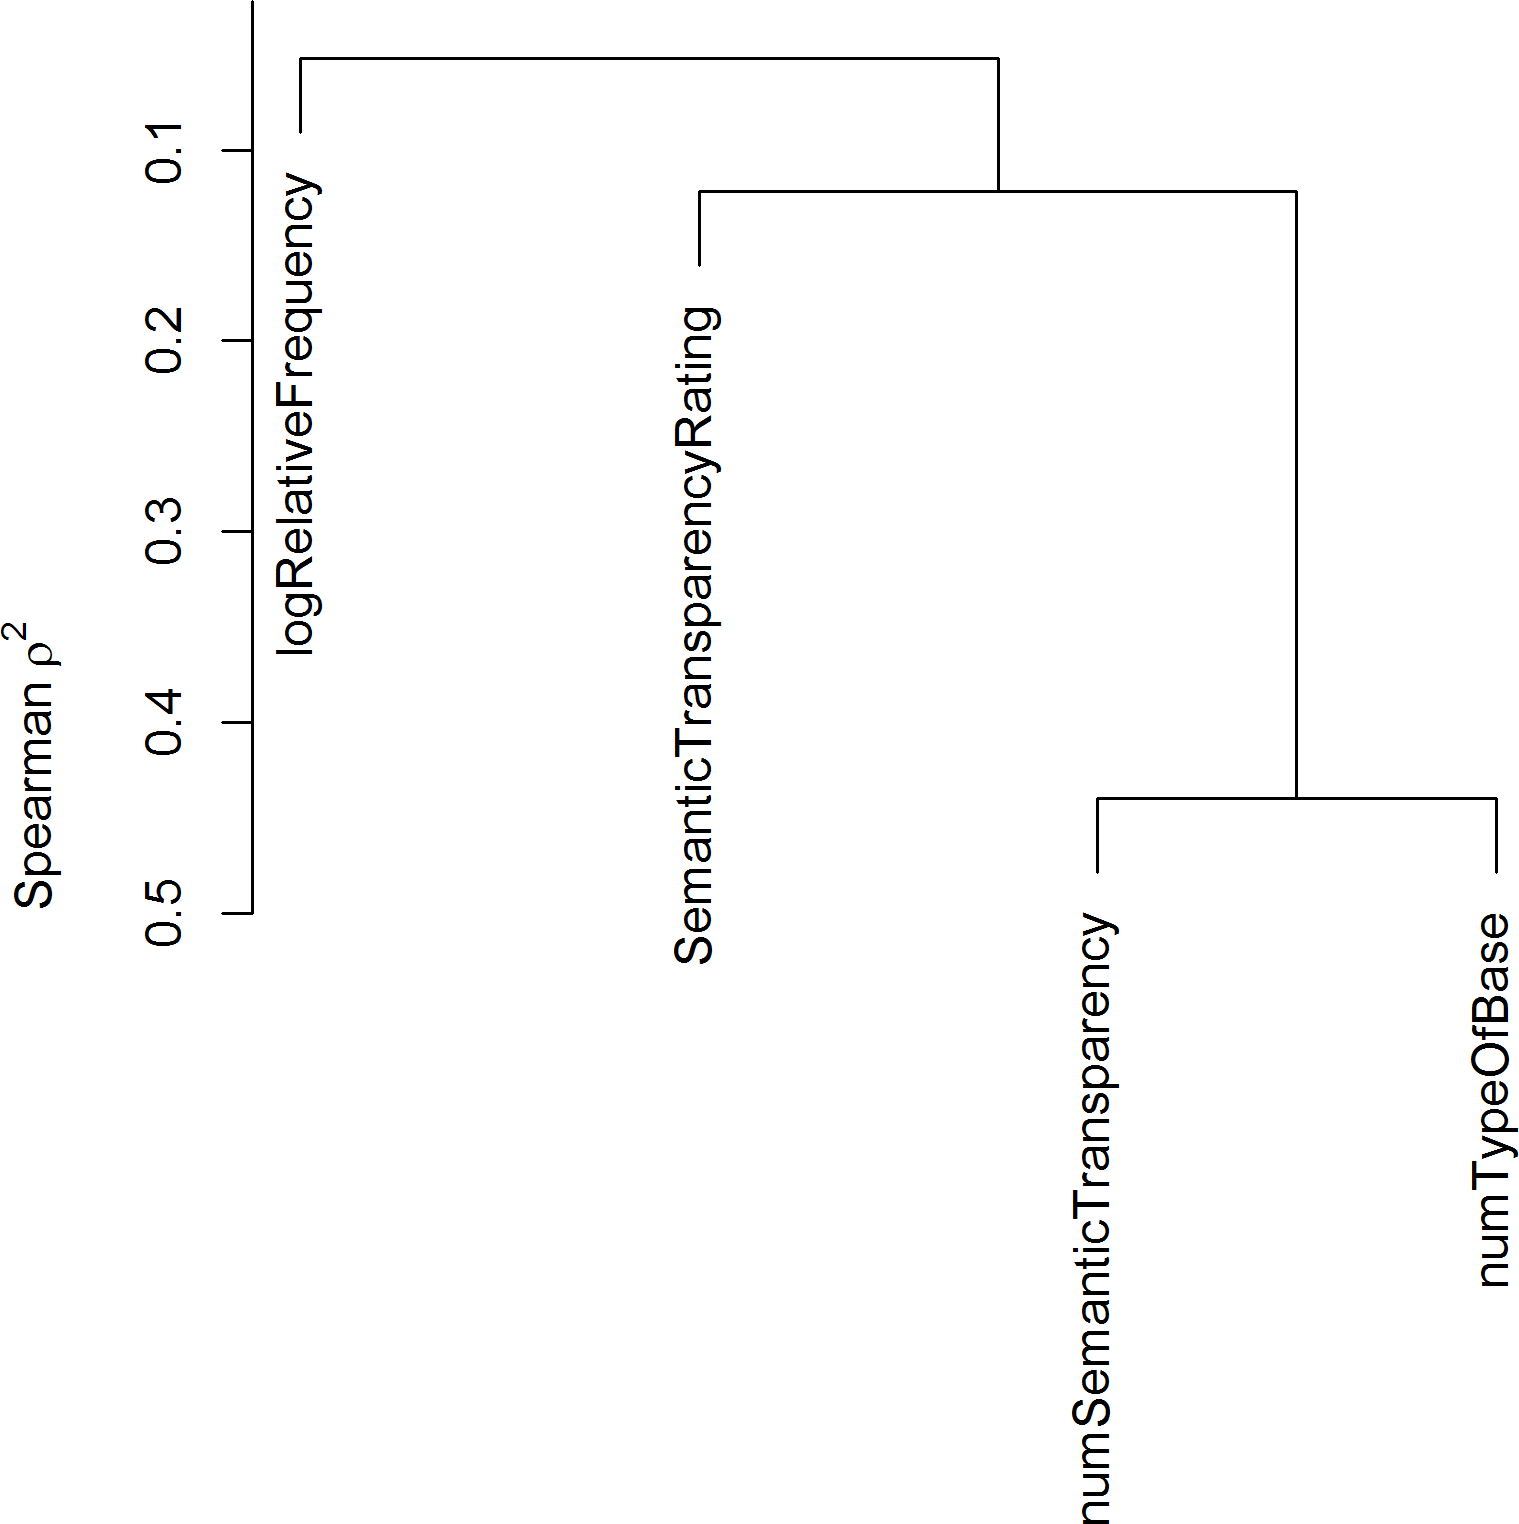
\includegraphics[scale=0.5]{images/Experiment/clusterAnalysisDecomposabilityExperimentAllTokens.png}
 	%\vspace*{-8mm} 
 	\caption{Dendrogram of the four decomposability measures for all words in the experimental study}
 	\label{fig:cluster experiment all affixes}
 \end{figure*}
 
\figref{fig:cluster experiment all affixes} displays the relation between the variables in a dendrogram. On the y-axis the squared Spearman correlation score between the variables is displayed. 
The figure shows two splits which structure the variables into three clusters. The lower the split in the figure is, the higher is the correlation between the variables of the pertinent cluster.
The first split is positioned in the upper part of the figure and separates the  variable log\textsc{RelativeFrequency} from all other variables. That log\textsc{RelativeFrequency} forms its own cluster in the upper part of the figure indicates the dissimilarity of this variable to the other \is{decomposability measure}decomposability variables. 
The second split, which is also positioned in the upper part of the figure, separates the variable \textsc{SemanticTransparencyRating} from \textsc{numSemanticTransparency} and \textsc{numTypeOfBase}. This indicates that \textsc{SemanticTransparencyRa-ting} is also rather dissimilar from the other \is{decomposability measure}decomposability variables. 
\textsc{numSemanticTransparency} and \textsc{numTypeOfBase} are much more similar to each other. This is indicated by the cluster they form in the lower part of the figure. 

 
 

 

  \begin{figure*}
  	
  	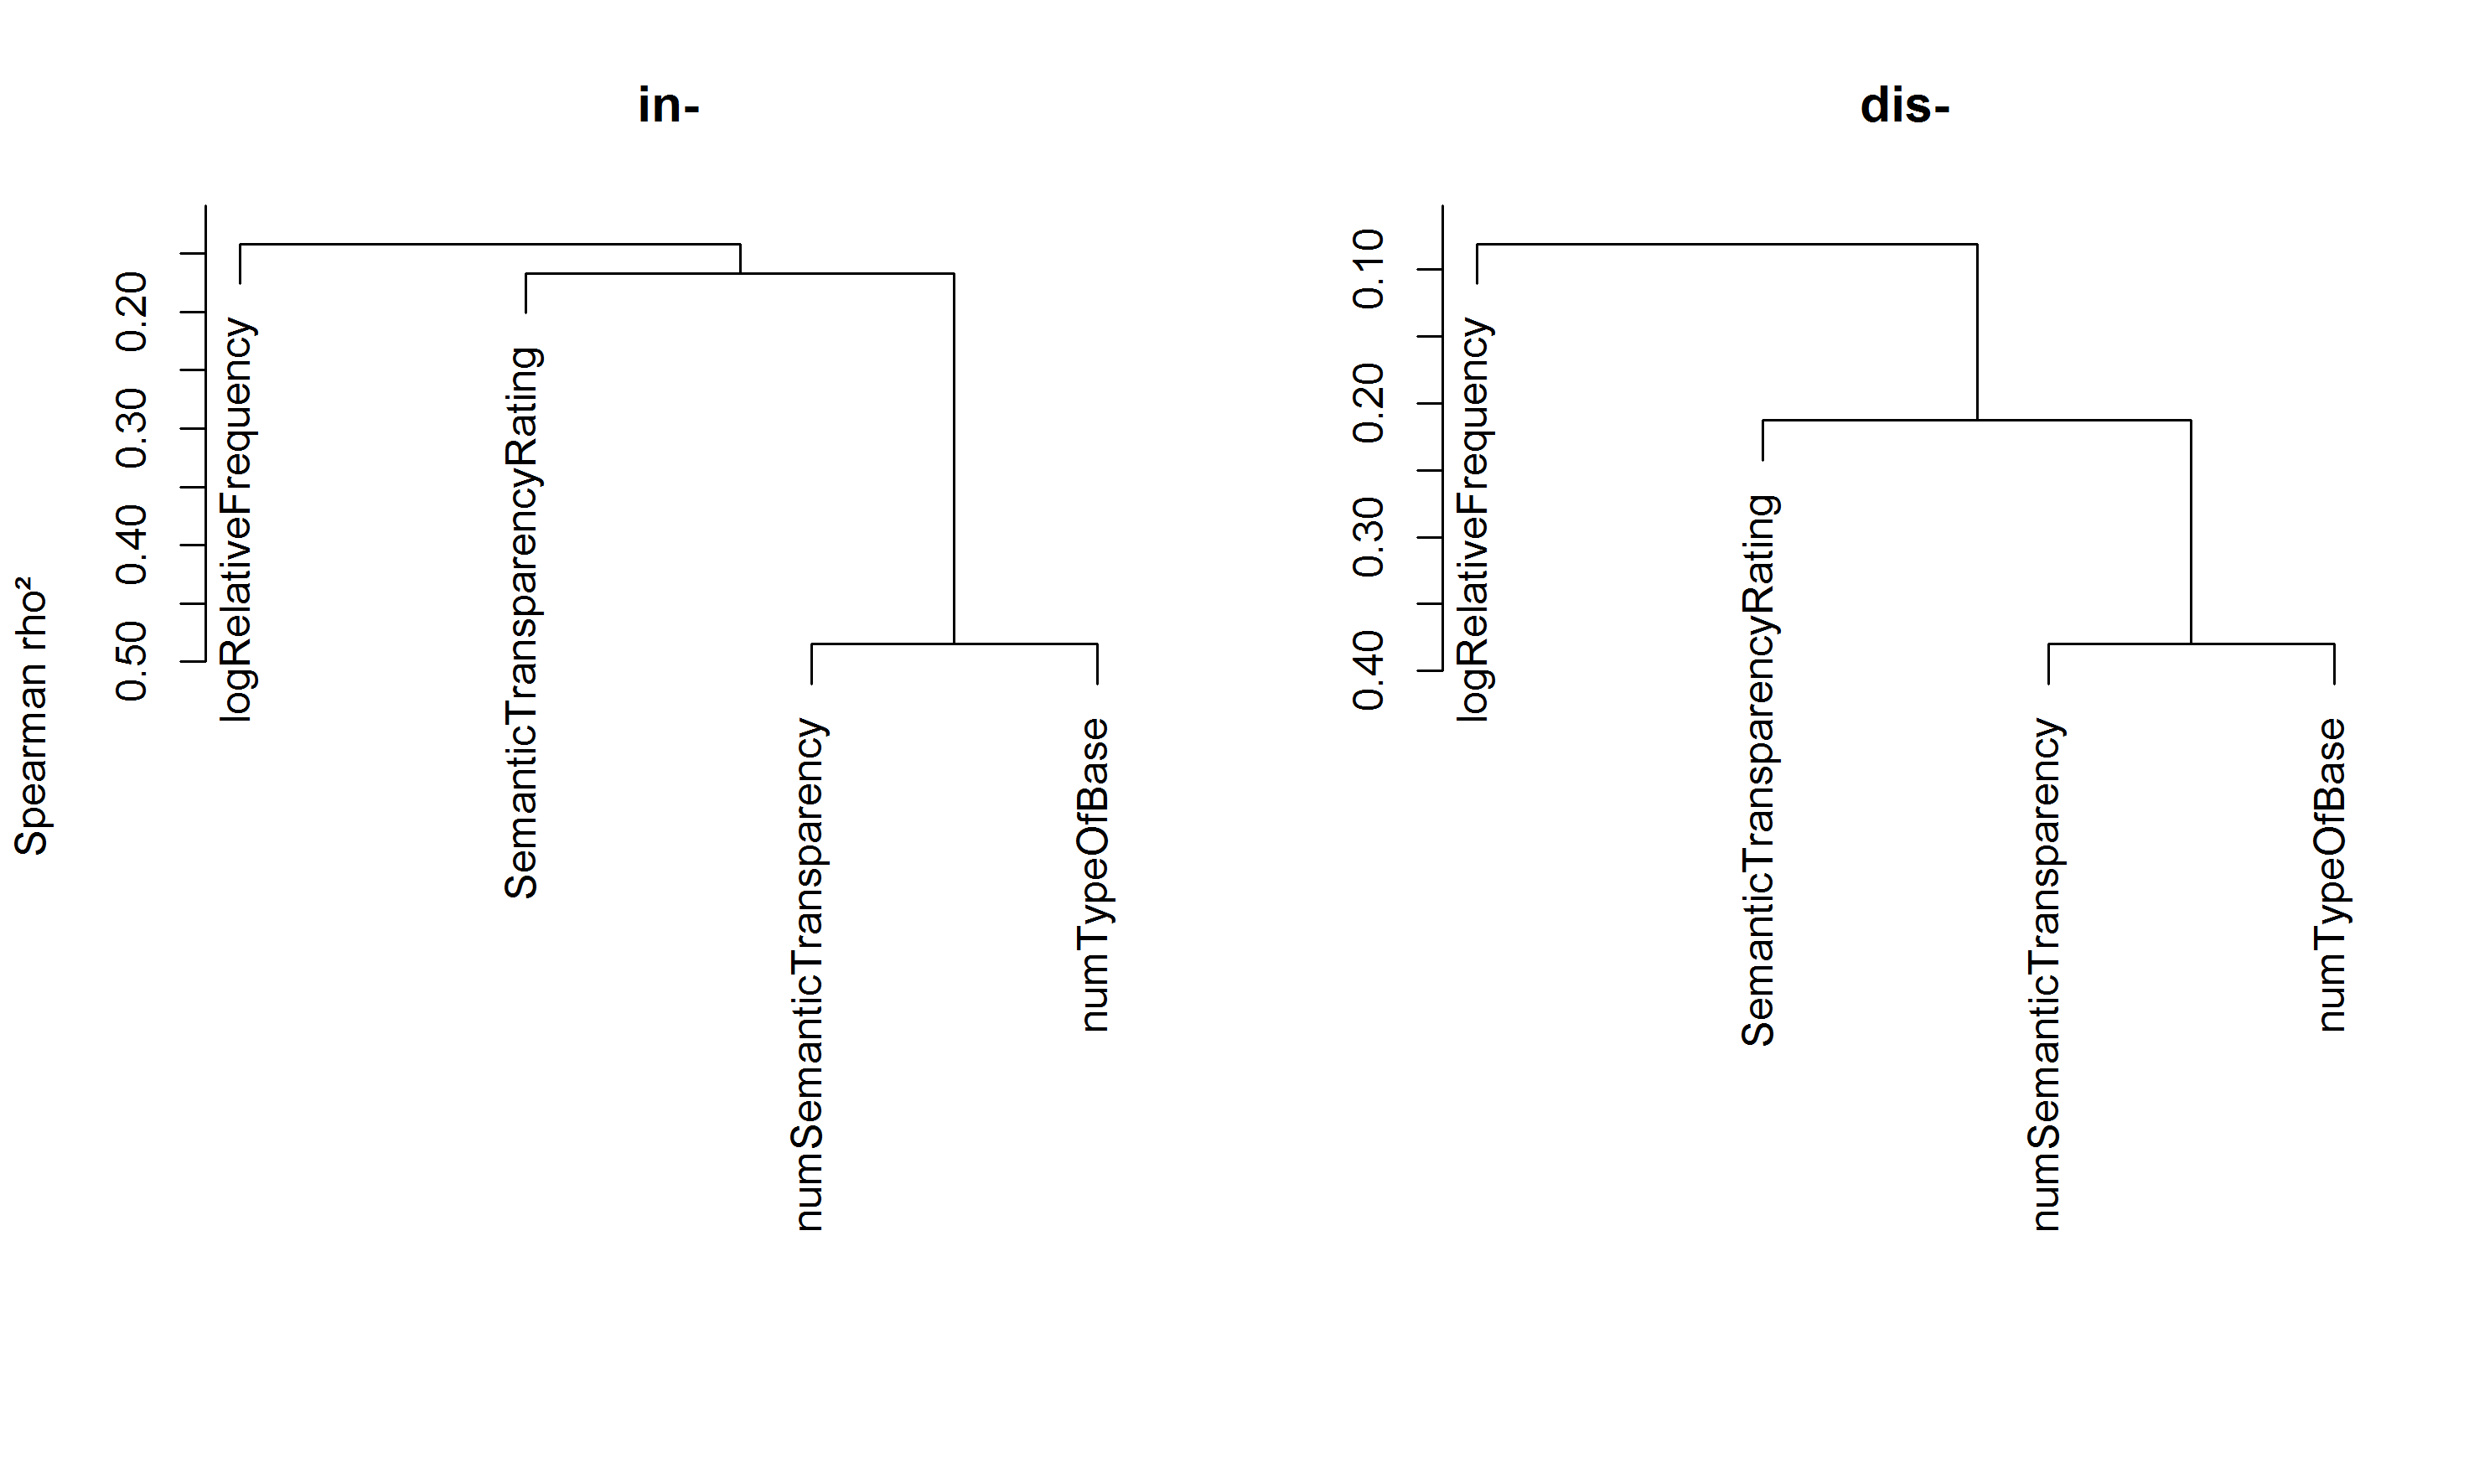
\includegraphics[scale=0.5]{images/Experiment/clusterAnalysisDecomposabilityExpDisAndIn.png}
  %	\vspace*{-20mm} 
  	\caption{Dendrogram of the four decomposability measures for \prefix{in} and \prefix{dis}prefixed words in the experimental study}
  	\label{fig:cluster experiment dis and in}
  	%	\vspace*{-10mm} 
  \end{figure*}
  
 The results of the \is{hierarchical cluster analysis}{cluster analyses} for \is{in-}\prefix{in} and \is{dis-}\prefix{dis} are displayed in the dendrograms in \figref{fig:cluster experiment dis and in}. The results resemble the result of the first \is{hierarchical cluster analysis}{cluster analysis}.
 For both prefixes, the variables \textsc{numSemanticTransparency} and \textsc{numTypeOfBase} cluster together in the lower part of the figure. This means that the correlations between these two variables are rather high. Log\textsc{RelativeFrequency} and \textsc{SemanticTransparencyRating} do not correlate to a high degree with any other variable.
 For \is{dis-}\prefix{dis}, \textsc{SemanticTransparencyRating} is a little more similar to \textsc{numSemanticTransparency} and \textsc{numTypeOfBase} than for \is{in-}\prefix{in}. 
 Overall, log\textsc{RelativeFrequency} and \textsc{SemanticTransparencyRating} are, however, not very similar to the other \is{decomposability measure}decomposability variables in both data sets. 

 
 To sum up, the \is{hierarchical cluster analysis}{cluster analyses} have revealed that the two variables \textsc{Semantic-Transparency} and \textsc{TypeOfBase} are very similar. The two variables log\textsc{Relative- Frequency} and \textsc{SemanticTransparancyRating}, in contrast, barely correlate with any other \isi{decomposability} variable.
This outcome only partly resembles the outcome of the corpus study. While both studies found that \textsc{SemanticTransparency} and \textsc{TypeOfBase} are very similar, and that the variable log\textsc{RelativeFre-quency} is different, the outcome for \textsc{SemanticTransparencyRating} differs between the studies. 
In the corpus study, \textsc{SemanticTransparencyRating} is very similar to \textsc{SemanticTransparency} and to \textsc{TypeOfBase}. In the experimental stu-dy, the correlations between \textsc{SemanticTransparencyRating} and \textsc{TypeOfBase}, and between \textsc{SemanticTransparencyRating}  and \textsc{SemanticTransparency} are not very high. They are barely higher than the ones between log\textsc{RelativeFre-quency} and the three other \is{decomposability measure}decomposability variables. 
This means that while ratings of the corpus study were highly influenced by the \isi{semantic transparency} and the type of base of a derivative, the ratings of the experimental study were less influenced by these factors.

 
 %Possible reasons for differences in ratings
 One possible explanation for this difference between the corpus and the experimental ratings is that the two groups of raters might have differed with regard to their definition of \isi{decomposability}, and that this difference might have led to different rating strategies. This explanation especially makes sense regarding the fact that the experimental raters were younger and mostly students, while the corpus raters represent a random selection of people of different ages. It might be the case that the younger raters, who are still in school, used a rule-based rating strategy which is based on their knowledge about word-formation, while the older raters, who might not have such knowledge, relied on information about \isi{semantic transparency} and the type of base of a word. 

 The relation between the \is{decomposability measure}decomposability measures has important implications for the interpretation of possible \isi{decomposability} effects on duration. As in the corpus study, possible effects of the \is{decomposability measure}decomposability variables \textsc{Semantic-Transparency} and \textsc{TypeOfBase} can be assumed to be caused by the same underlying property. 
 Effects of log\textsc{RelativeFrequency} and \textsc{SemanticTransparencyRating} on duration are probably caused by different underlying properties (see also \sectref{The Relation between Decomposability Measures} for a discussion of the concept \isi{decomposability} and its operationalization in the study).
 





\begin{table}
	\begin{tabularx}{\textwidth}{p{2.25cm}lQ}
	\lsptoprule
	& Segmentability hierarchy &	Additional assumption\\
		\midrule
	Semantic\newline Hierarchy & \prefix{un} > \{\prefix{dis}, \prefix{in}\textsubscript{\textsc{Neg}}\}>  \prefix{in}\textsubscript{\textsc{Loc}} > \suffix{ly}& lexical meaning over productivity, transparency and type of base \\\tablevspace
	Non-Semantic Hierarchy	&  	\prefix{un} > \suffix{ly} > \{\prefix{dis}, \prefix{in}\textsubscript{\textsc{Neg}}\}>  \prefix{in}\textsubscript{\textsc{Loc}}& productivity, transparency and  type of base	over lexical meaning \\
	\lspbottomrule
\end{tabularx}
	\caption{Lexical segmentability hierarchies of  affixes\label{fig:Segmentability hierarchies of  affixes repetition 3}\is{productivity}}
\end{table}


\subsection{The segmentability of the affixes: A comparison} \label{Exp The Segmentability of the Affixes: A Comparison}
\tabref{fig:Segmentability hierarchies of  affixes repetition 3} displays the \isi{segmentability} hierarchies proposed in \sectref{comparison affixes}. To see whether the hierarchies are borne out by the data, it is necessary to compare the \isi{segmentability} of the five investigated affixes as found in the data. If the hierarchies are valid, the \isi{segmentability} of the affixes should pattern according to the hierarchies. 
As explained above, in the experimental study, only the distribution of the variable \textsc{SemanticTransparencyRating} across affixes was compared to investigate the \isi{segmentability} of the affixes.


\tabref{tbl:Exp distribution semantic transparency rating} shows the distribution of \textsc{SemanticTransparencyRating} for each affix. Next to the total number of tokens, the percentage of tokens with the pertinent rating per affix is given. 


\begin{table}
	\caption{Semantic Transparency Rating  by affix\label{tbl:Exp distribution semantic transparency rating}}
    \resizebox{\textwidth}{!}{%		
		\begin{tabular} {lr@{ }rr@{ }rr@{ }rr@{ }rr@{ }r}
            \lsptoprule
			\textsc{SemanticTrans-}& & & &&   \\
			\textsc{parencyRating }&\multicolumn{2}{c}{\prefix{in}\textsubscript{\textsc{Loc}}  }&\multicolumn{2}{c} {\suffix{ly}} & \multicolumn{2}{c} {\textit{dis-}} & \multicolumn{2}{c} {\prefix{in}\textsubscript{\textsc{Neg}} }   & \multicolumn{2}{c} {\prefix{un} }   \\
			\midrule
			
			1 - most decomposable             &  201 &(35\%) &   747& (62\%)  &   590& (71\%)    & 1225 &(71\%)   & 1868& (92\%)        \\
			2                                 &  81  &(14\%) &   213&(18\%)   & 119&(14\%) &  244&(14\%)&   129&(6\%)  \\
			3								  &  100 &(17\%) &   182&(15\%)   &   69&(8\%)&  148&(9\%) & 37&(2\%)    \\
			4 -  least decomposable           &  194 &(34\%) &    63&(5\%)    & 51&(6\%) &  100&(6\%) &  5 &(\textless 1\%)  \\
			\lspbottomrule			
		\end{tabular}}
\end{table}

%Results
Overall most  items were rated as quite easy to decompose, i.e. the majority of items was rated with 1. This distribution supports the suspicion that experimental raters might have used a rule-based approach in their rating, i.e. they categorically rated items as either decomposable or not decomposable. 
However, the table also shows that there is variation in the ratings. 
Crucially, there are differences in the distribution of ratings between affixes. Kruskal-Wallis tests ($p<0.05$) revealed that all differences between affixes, except the one between \is{negative in-}negative \prefix{in} and \is{dis-}\prefix{dis}, are significant.



The prefix \is{un-}\prefix{un} is rated as the most segmentable affix. 
 Locative \prefix{in} is rated as the least segmentable affix, and the other three affixes pattern in between. 
  This pattern partly resembles the pattern found in the corpus study. In both studies, \is{un-}\prefix{un} was rated the most segmentable affix, and \is{locative in-}locative \prefix{in} was rated the least segmentable affix. 
 However, differently from the corpus study, in the experimental study, the suffix \is{-ly}\suffix{ly} is rated as slightly less decomposable than \is{negative in-}negative \prefix{in} and \is{dis-}\prefix{dis}. In the corpus study, \is{-ly}\suffix{ly} was rated as the second most segmentable affix after \is{un-}\prefix{un}.


The difference in the rating of the suffix \is{-ly}\suffix{ly} between corpus and experimental rating is very interesting with regard to the \isi{segmentability} status of the suffix and the \isi{segmentability} hierarchies. The placement of \is{-ly}\suffix{ly} in the \isi{segmentability} hierarchies highly depends on the definition of \isi{decomposability}. On the one hand, \is{-ly}\suffix{ly} is very segmentable in terms of its \isi{productivity}, its transparency and the types of bases it takes, on the other, the suffix does not feature a clear lexical meaning and its status as a derivational suffix is contested in the literature (see, for example, \citealt{Zwicky.1995}; \citealt{Plag.2003}; \citealt{Giegerich.2012}; \citealt{Bauer.2013} for discussion). Depending on one's definition of \isi{decomposability}, \is{-ly}\suffix{ly} is either a very segmentable affix (Non-Semantic Segmentability Hierarchy) or an affix with very low \isi{segmentability} (Semantic Segmentability Hierarchy) (see also discussion in \sectref{ly}). 

The different \isi{segmentability} patterns found in the corpus and the experimental study mirror the ambiguous \isi{segmentability} status of \is{-ly}\suffix{ly}. In turn, they can be interpreted to provide support for the validity of both \isi{segmentability} hierarchies. 
In the corpus study, the suffix \is{-ly}\suffix{ly} is the second most segmentable affix. This is in line with the Non-Semantic Segmentability Hierarchy. 
In the experimental study, the suffix \is{-ly}\suffix{ly} is rated as one of the least segmentable affixes. This is in line with the Semantic Segmentability Hierarchy.\footnote{Note, however, that according to the Semantic Segmentability Hierarchy, \is{locative in-}locative \prefix{in} is expected to be less segmentable than \is{-ly}\suffix{ly}. This is not the case. }
The \isi{segmentability} pattern of the prefixes provides further support for the validity of the two hierarchies. In both studies, the \isi{segmentability} of the prefixes patterns according to both hierarchies. 



\subsection{Summary}

% Summary
The investigation of the relation of the \is{decomposability measure}decomposability measures has revealed that while the two variables \textsc{SemanticTransparency} and \textsc{TypeOfBase} are very similar to each other, the two variables log\textsc{RelativeFrequency} and \textsc{Semantic-TransparencyRating} are different from all other \is{decomposability measure}decomposability measures.
This has important implications for the interpretation of possible \isi{decomposability} effects on duration. While possible effects of \textsc{SemanticTransparency} and \textsc{TypeOfBase} can be assumed to be caused by the same underlying property, possible effects of log\textsc{RelativeFrequency} and \textsc{SemanticTransparencyRating} on duration are probably caused by different underlying properties.



With regard to the \isi{segmentability} of the affixes, the experimental rating shows a similar pattern as the corpus study. As in the corpus study, the prefix \is{un-}\prefix{un} is rated as the most segmentable affix, and \is{locative in-}locative \prefix{in} is rated as the least segmentable affix. However, the suffix \is{-ly}\suffix{ly} is rated differently in the experimental rating, i.e. it is the second least segmentable affix, whereas it is rated the second most segmentable affix in the corpus. The different ratings for \is{-ly}\suffix{ly} in the corpus and the experimental study mirror the ambiguous \isi{segmentability} status of the affix and its different placements in the \isi{segmentability} hierarchies. 



\section{Duration}


\subsection{Analyses} \label{analsyses duration experiment}

As in the corpus study, each affix (and each allomorph, if there was more than one) was investigated separately, i.e. five subsets were created, one for the \is{un-}\prefix{un} words, one for the /ɪn/-words, one for the \is{im-}/ɪm/ -words, one for the \is{dis-}\prefix{dis}words, and one for the \is{-ly}\suffix{ly}-words.

To get a first impression of the \isi{gemination} pattern, and to test whether \isi{gemination} is a categorical or a gradient phenomenon, the first durational analysis consisted of investigating the raw distribution of consonant duration in each subset (cf. \textit{Nature of {gemination}: Predictions }in \sectref{predictions nature of gemination}). To see whether the distributions differ between environments, I generated boxplots for each environment of each subset. 
If the boxplots indicate a bimodal distribution with doubles having a higher mean than singletons, one can assume \isi{gemination} to be categorical (see \sectref{analyses dur corpus} for detailed description of the analyzing strategy). 

After investigating the raw distributions across environments, I fitted two linear mixed effects \is{regression model}{regression models} to each subset. 
The first model predicts \is{absolute duration}absolute consonant duration with all complex words of a given subset (\textit{complex model}). These models are very similar to the models fitted in the corpus study, i.e. they include complex words with a phonological double (e.g. \textit{unnatural}) and complex words with a phonological singleton (e.g. \textit{uneasy}). 
The second model, the \textit{complete model,} predicts \is{absolute duration}absolute consonant duration with all tokens of a pertinent subset, i.e. the models also include base words with a singleton (e.g. \textit{natural} or \textit{real}), and simplex words with an orthographic double (e.g. \textit{dissertation} or \textit{belly}). The complete models were fitted to test whether phonological doubles are longer than corresponding singletons in base words, and whether \isi{gemination} is affected by the presence of orthographic doubles. 

In addition to the two models for each subset, one model which directly compares \is{un-}\prefix{un} and /ɪn/-prefixed words was fitted. This model was fitted to test whether the three prefixes \is{un-}\prefix{un}, \is{locative in-}locative \prefix{in} and \is{negative in-}negative \prefix{in} deviate in their durational patterns. No other affixes were directly compared in one model as inherent durational differences between different types of consonants are too severe to be investigated in one model. Note that in the model featuring \is{un-}\prefix{un} and /ɪn/-prefixed words, some variables cannot be investigated because there are systematic differences in the distribution of variables between the prefixes. Details will be given in the pertinent section.


The dependent variable of all models was \is{absolute duration}absolute consonant duration. Based on the findings of the corpus study, no models with \isi{relative duration} as the dependent variable were fitted.  The corpus study revealed that relative consonant duration is a much weaker measure of \isi{morphological gemination} in English than \is{absolute duration}absolute consonant duration (see \sectref{Summary Corpus Study}).

Only the complex models tested the effects of the \is{decomposability measure}decomposability measures on consonant duration, since the \is{decomposability measure}decomposability variables are not applicable to simplex words.
Furthermore, not all \is{decomposability measure}decomposability measures were tested for all affixes. As in the corpus study, only in the complex  \is{in-}\prefix{in} and \is{dis-}\prefix{dis}models all \is{decomposability measure}decomposability variables were included. In the complex \is{-ly}\suffix{ly}-model, only the effects of log\textsc{RelativeFrequency} and \textsc{SemanticTransparencyRating} were tested. In the complex \is{un-}\prefix{un}model, only the effect of log\textsc{RelativeFrequency} was tested. The reason is that the two variables  \textsc{SemanticTransparency} and \textsc{TypeOfBase} do not show enough variation for \is{un-}\prefix{un} and \is{-ly}\suffix{ly}. For \is{un-}\prefix{un}, \textsc{SemanticTransparencyRating} does not show enough variation either.


In the complex models predicting consonant duration with /ɪn/, \is{im-}/ɪm/  and \is{dis-}\prefix{dis}, \isi{collinearity} problems had to be addressed. As discussed in the previous section, the \is{decomposability measure}decomposability variables \textsc{SemanticTransparency} and \textsc{TypeOfBase} highly correlate, and there are also correlations between the other \is{decomposability measure}decomposability variables. It is thus problematic to test all of them simultaneously in the model. Therefore, the effect of these variables was tested by including them individually in the model, and by conducting \is{principal component analysis}principal component analyses (see \sectref{stats} on \is{principal component analysis}principal component analyses). 

In the complete models for the prefixes, the noise variable \textsc{PrecedingSegmentDuration} was not included because the base-initial consonant does not feature a preceding segment. In all models, the two variables \textsc{Speaker} and \textsc{Type} were included as random effects.


As in the corpus study, two types of interactions were tested in each model. First, I tested for interactions which are predicted to affect \isi{gemination} according to the theoretical approaches discussed in Chapter \ref{Theory}. Then, I tested for interactions which, based on previous empirical work and theoretical considerations, can be assumed to affect affixational consonant duration  (see \sectref{analyses dur corpus} for a more detailed description of the two types of interactions). 
 All interactions tested in the experimental study are listed in \hyperref[Appendix G Summaries of tested interactions in experimental study]{Appendix G}.

All models were fitted according to the modeling strategy described in \sectref{stats}.  
The models were generated using the \texttt{lme4 package} (\citealt{Bates.2014}), and the plots of the \is{regression model}{regression models} were generated with the \texttt{visreg package} (\citealt{Breheny.2015}). 

After fitting the complex models for each subset, I computed each variable's contribution to the goodness of fit for the final model by checking how the absence of each significant term affects the AIC of the model. The higher the increase of the AIC without a specific term, the more variance is explained by the pertinent term in the model, and the higher is its contribution to the goodness of fit.







\subsection{Overview}
	
\figref{fig:Expeirment raw duration distribution} depicts the distribution of consonant duration for each environment in each subset using boxplots. In the upper row, the distribution for \is{un-}\prefix{un} is shown in the left panel, the one for /in/
%\todo{do you mean /in/ or /ɪn/?} 
is shown in the middle panel, and the one for \is{im-}/ɪm/  is shown in the right panel. The distribution for \is{dis-}\prefix{dis} is shown in the lower left panel, and the one for \is{-ly}\suffix{ly} in the lower right panel.
The y-axis of each plot displays the duration of the consonant in milliseconds. 

The boxes in each plot represent the distribution of consonant duration for the different environments in each data set. The dot in the middle represents the median duration, and the box itself represents the interquartile range of consonant duration. 
In each plot, the left box(es) represent the environment(s) with a phonological double. They are followed by the box(es) for  complex words with singleton environments and the box(es) for base words with a singleton. For \is{dis-}\prefix{dis} and \is{-ly}\suffix{ly}, the last box (from the left) represents the consonant duration in simplex words with an orthographic double.




\begin{figure*}
	
	\begin{subfigure}
		
		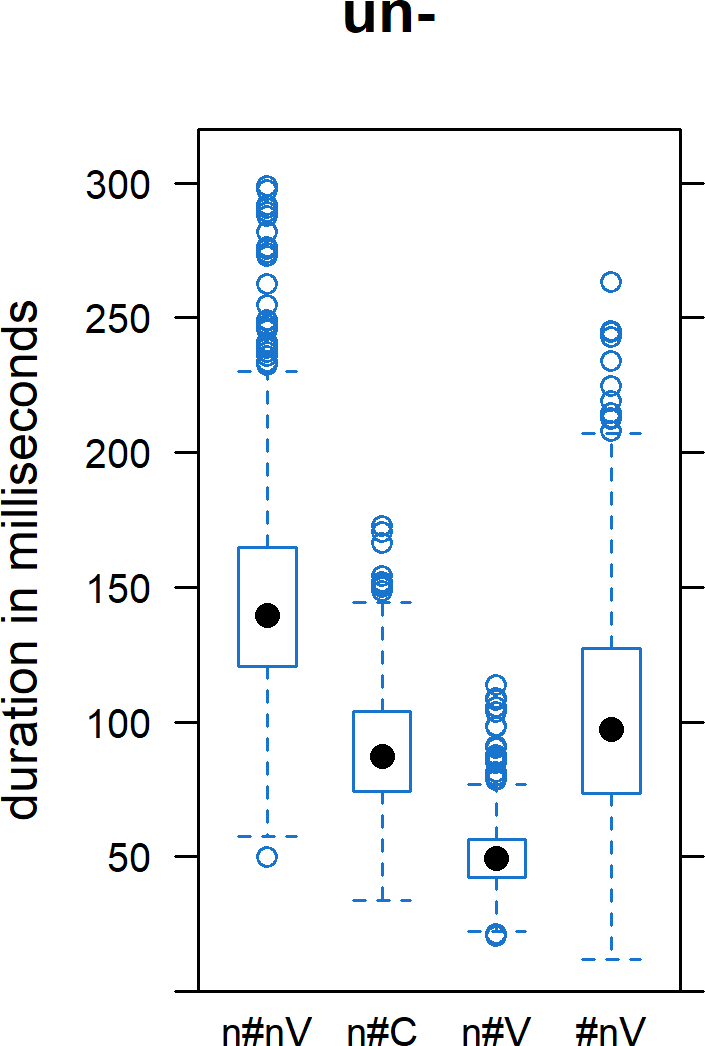
\includegraphics[scale=.55]{images/Experiment/boxUn}
		%	\caption{1a}
		%	\label{fig:sfig1}
	\end{subfigure}%
	~
	\begin{subfigure}
		
		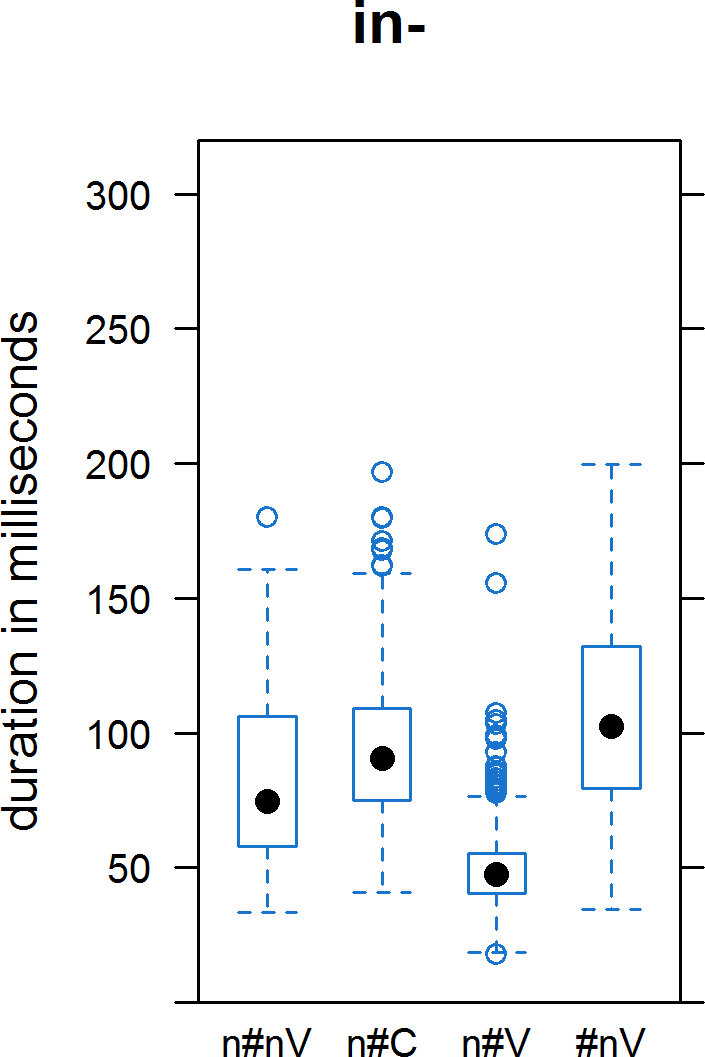
\includegraphics[scale=.55]{images/Experiment/boxIn}
		%	\caption{1b}
		%	\label{fig:sfig2}
	\end{subfigure}
	~
	\begin{subfigure}
		
		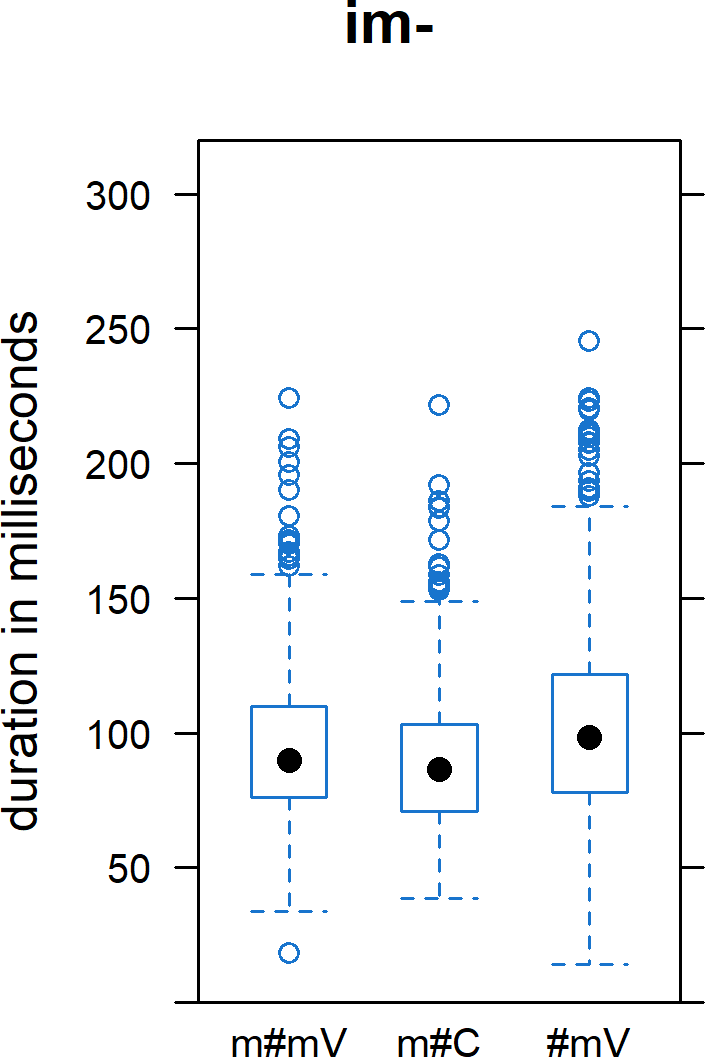
\includegraphics[scale=.55]{images/Experiment/boxIm}
		%	\caption{1b}
		%	\label{fig:sfig2}
	\end{subfigure}
	
	\begin{subfigure}
		
		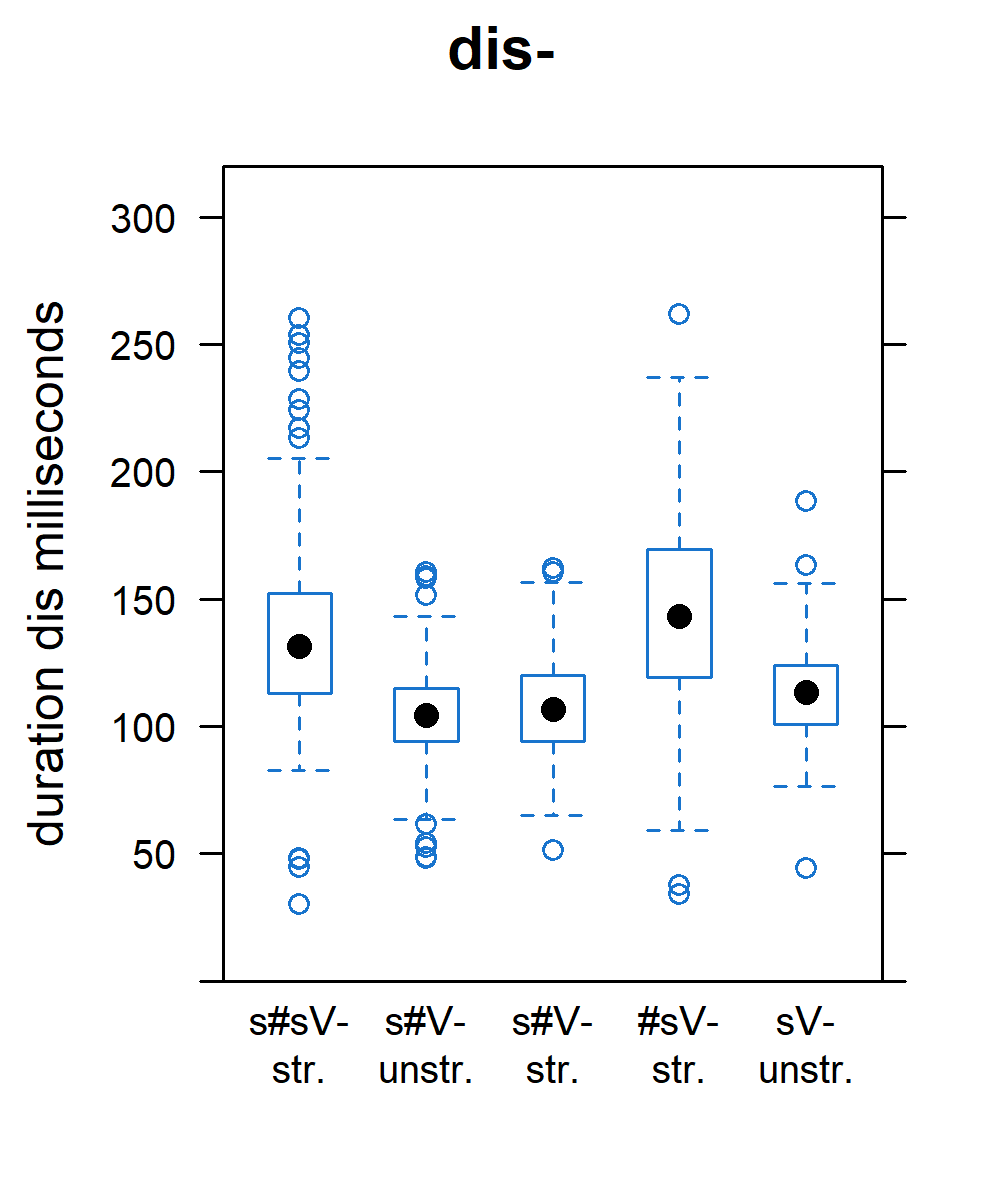
\includegraphics[scale=.55]{images/Experiment/boxDis}
		%	\caption{1b}
		%	\label{fig:sfig2}
	\end{subfigure}
	~
	\begin{subfigure}
		
		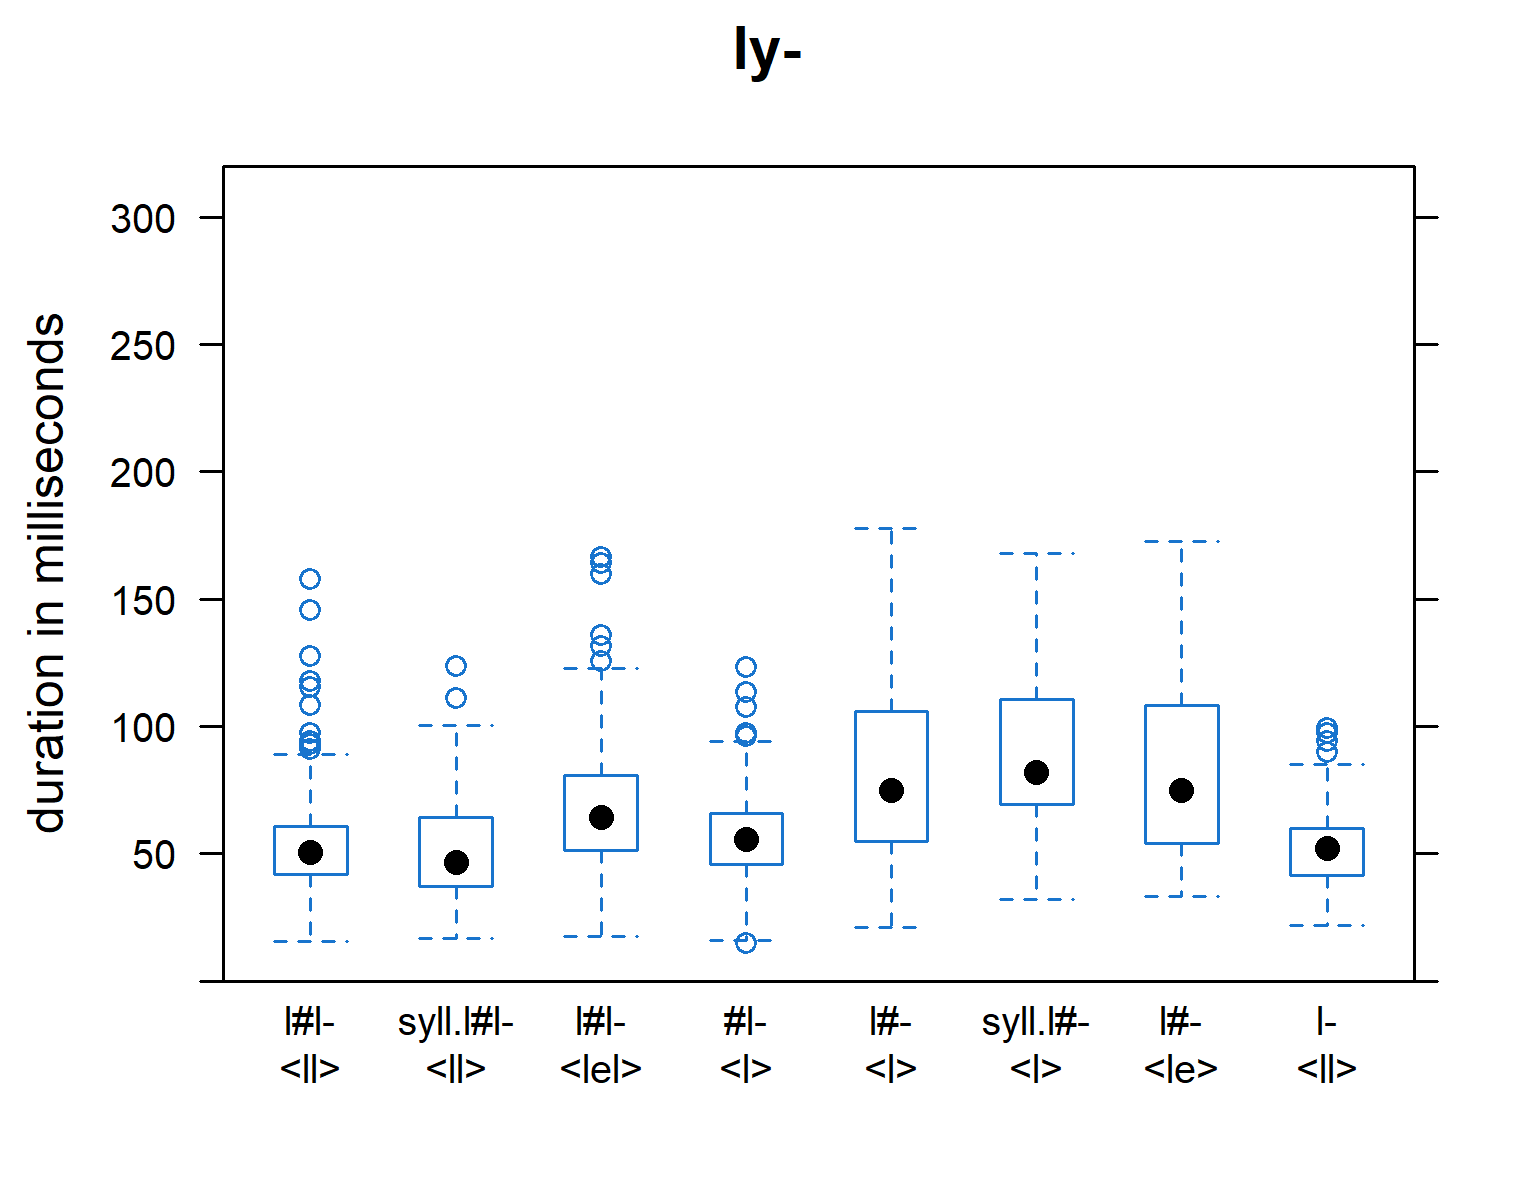
\includegraphics[scale=.55]{images/Experiment/boxLy}
		%	\caption{1b}
		%	\label{fig:sfig2}
	\end{subfigure}				
	
	\caption{Distribution of consonant duration in the five data sets}
	\label{fig:Expeirment raw duration distribution}
\end{figure*}



%un
%plot
For \is{un-}\prefix{un},  the figure shows a clear difference in duration between double and single consonants. Doubles (\texttt{n\#nV}) are longer than singletons in complex words (\texttt{n\#C}, \texttt{n\#V}) and singletons in base words (\texttt{\#nV}). 
  The figure also shows that there is no overlap of the boxes for the doubles and the boxes for the singletons. This indicates a bimodal distribution in the data set with doubles being longer than singletons. 
As the data from the corpus study, the  plot thus suggests that \is{un-}\prefix{un} geminates, and that \isi{gemination} is a categorical phenomenon. 



%in
For /ɪn/, the plot suggests that doubles (\texttt{n\#nV}) are as long as the singletons in complex words followed by a consonant (\texttt{n\#C}) and singletons in base words (\texttt{\#nV}). Only singletons in complex words followed by a vowel (\texttt{n\#V}) are shorter than doubles. 
On the one hand, this durational difference speaks for \isi{gemination} with \is{in-}\prefix{in}, on the other, there is no durational difference between the other singleton levels and the double consonant. This is different from what was found for \is{un-}\prefix{un}.
With regard to the question whether \isi{gemination} is a categorical or a gradient phenomenon, the plot shows that there is no overlap between the box of the doubles (\texttt{n\#nV}) and the box of the singletons with a following vowel (\texttt{n\#V}) for /ɪn/. In other words, the distribution of duration of doubles and singletons with a following vowel seems to be bimodal. This suggests that, if there is \isi{gemination} with /ɪn/, it is probably categorical.

%im
For \is{im-}/ɪm/, no difference in consonant duration can be seen between the three environments (\texttt{m\#mV}, \texttt{m\#C}, \texttt{\#mV}). The plot thus suggests \isi{degemination} with \is{im-}/ɪm/. However, 
it is yet unclear whether the allomorph \is{im-}/ɪm/  really degeminates, or whether \isi{gemination} with \is{im-}/ɪm/  depends on additional factors which are not taken into account when comparing the raw durations of doubles and singletons. 

%dis

For \is{dis-}\prefix{dis}, the plot shows that doubles (\texttt{s\#sV-str.})  are longer than singletons in complex words (\texttt{s\#V-unstr.}, \texttt{s\#V-str.}) and singletons in simplex words with an orthographic double (\texttt{sV-unstr.}). However, singletons in base words (\texttt{\#sV}) are as long as doubles. 
As for /ɪn/, there is thus some evidence for \isi{gemination}, but also some evidence against it.  
The boxes for the double consonants and  for the singleton environments (except for the one for singletons in base words)  hardly overlap. Thus, the distribution of duration of doubles and singletons in complex words seems to be bimodal. This suggests that if there is \isi{gemination} with \is{dis-}\prefix{dis}, it is categorical.


%ly

For \is{-ly}\suffix{ly}, there is a big overlap in the distribution of all environments. Only singletons in base words (\texttt{l\#-<l>}, \texttt{syll.l\#-<l>}, \texttt{l\#-<le>}) seem to have slightly longer durations than singletons in all other environments. Crucially, the plot does not suggest doubles to be longer than singletons of any category. One might thus suspect \isi{degemination} for \is{-ly}\suffix{ly}. 

The overview of the durations of all environments reveals some similarities across all subsets, as well as some differences. 
One similarity is that in all subsets, the consonant in base words is relatively long. This might be due to its word-initial (or word-final) position. 
Furthermore, for the prefixes with a nasal, the nasal is longer before consonants than before vowels. 
Another similarity is that if there are differences between double and singleton consonants, their duration seems to be bimodally distributed. As in the corpus study, the data thus suggest \isi{gemination} to be a categorical phenomenon.

With regard to the question of \isi{gemination}, the affixes seem to behave quite differently. For \is{un-}\prefix{un}, the distributional analysis clearly suggests \isi{gemination}, doubles are longer than all singleton levels. 
For the other affixes, it is less clear whether we find \isi{gemination}. For \is{in-}\prefix{in}, i.e. /ɪn/ and \is{im-}/ɪm/, only one singleton environment features shorter consonants than the double environment.
For \is{dis-}\prefix{dis}, the singleton consonants of all but one environment are shorter than the double consonants. 
For \is{-ly}\suffix{ly}, none of the three double environments is longer than the singleton environments. Further analyses which take more variables into account are needed to clarify the \isi{gemination} pattern of the affixes. 
 In the next subsections I will present such analyses for each subset.


\subsection{The prefix \textit{un-}} \label{un experiment}

\subsubsection{Complex model}


The model predicting consonant duration with all complex \is{un-}\prefix{un}words ($N=2067$) was fitted according to the modeling procedure described in \sectref{stats}. Due to an uneven distribution of the residuals in the initial model, the dependent variable \textsc{AbsoluteConsonantDuration} was Box-Cox-transformed ($\lambda = 0.101$) and 50 outliers were removed (2.4\% of the data).
 After the model was refitted with the transformed dependent variable, it showed a satisfactory distribution of residuals.  The model was then simplified and interactions were tested (see \hyperref[Appendix G Summaries of tested interactions in experimental study]{Appendix G} for a list of all tested interactions).
 
After model simplification five variables remained in the model, \textsc{Environment}, \textsc{Accentuation}, \textsc{LocalSpeechRate}, \textsc{PrePause} and \textsc{PrecedingSegmentDuration}. The two variables \textsc{Environment} and \textsc{Accentuation} interact. The final model is summarized in \tabref{model un complex experiment} which can be found in \hyperref[Appendix H: Model Summaries Experiment]{Appendix H}.


The four noise variables show the expected effects. As in the corpus study, the nasal in \is{un-}\prefix{un} becomes shorter with increasing \isi{speech rate}. 
The nasal in tokens which are preceded by a pause is longer than the nasal in tokens without a preceding pause. This effect of \textsc{PrePause}  can be attributed to \isi{word-initial strengthening}.  
Furthermore, consonant duration depends on the duration of the preceding segment. The longer the preceding segment, the shorter the nasal. 

\begin{figure*}
	
	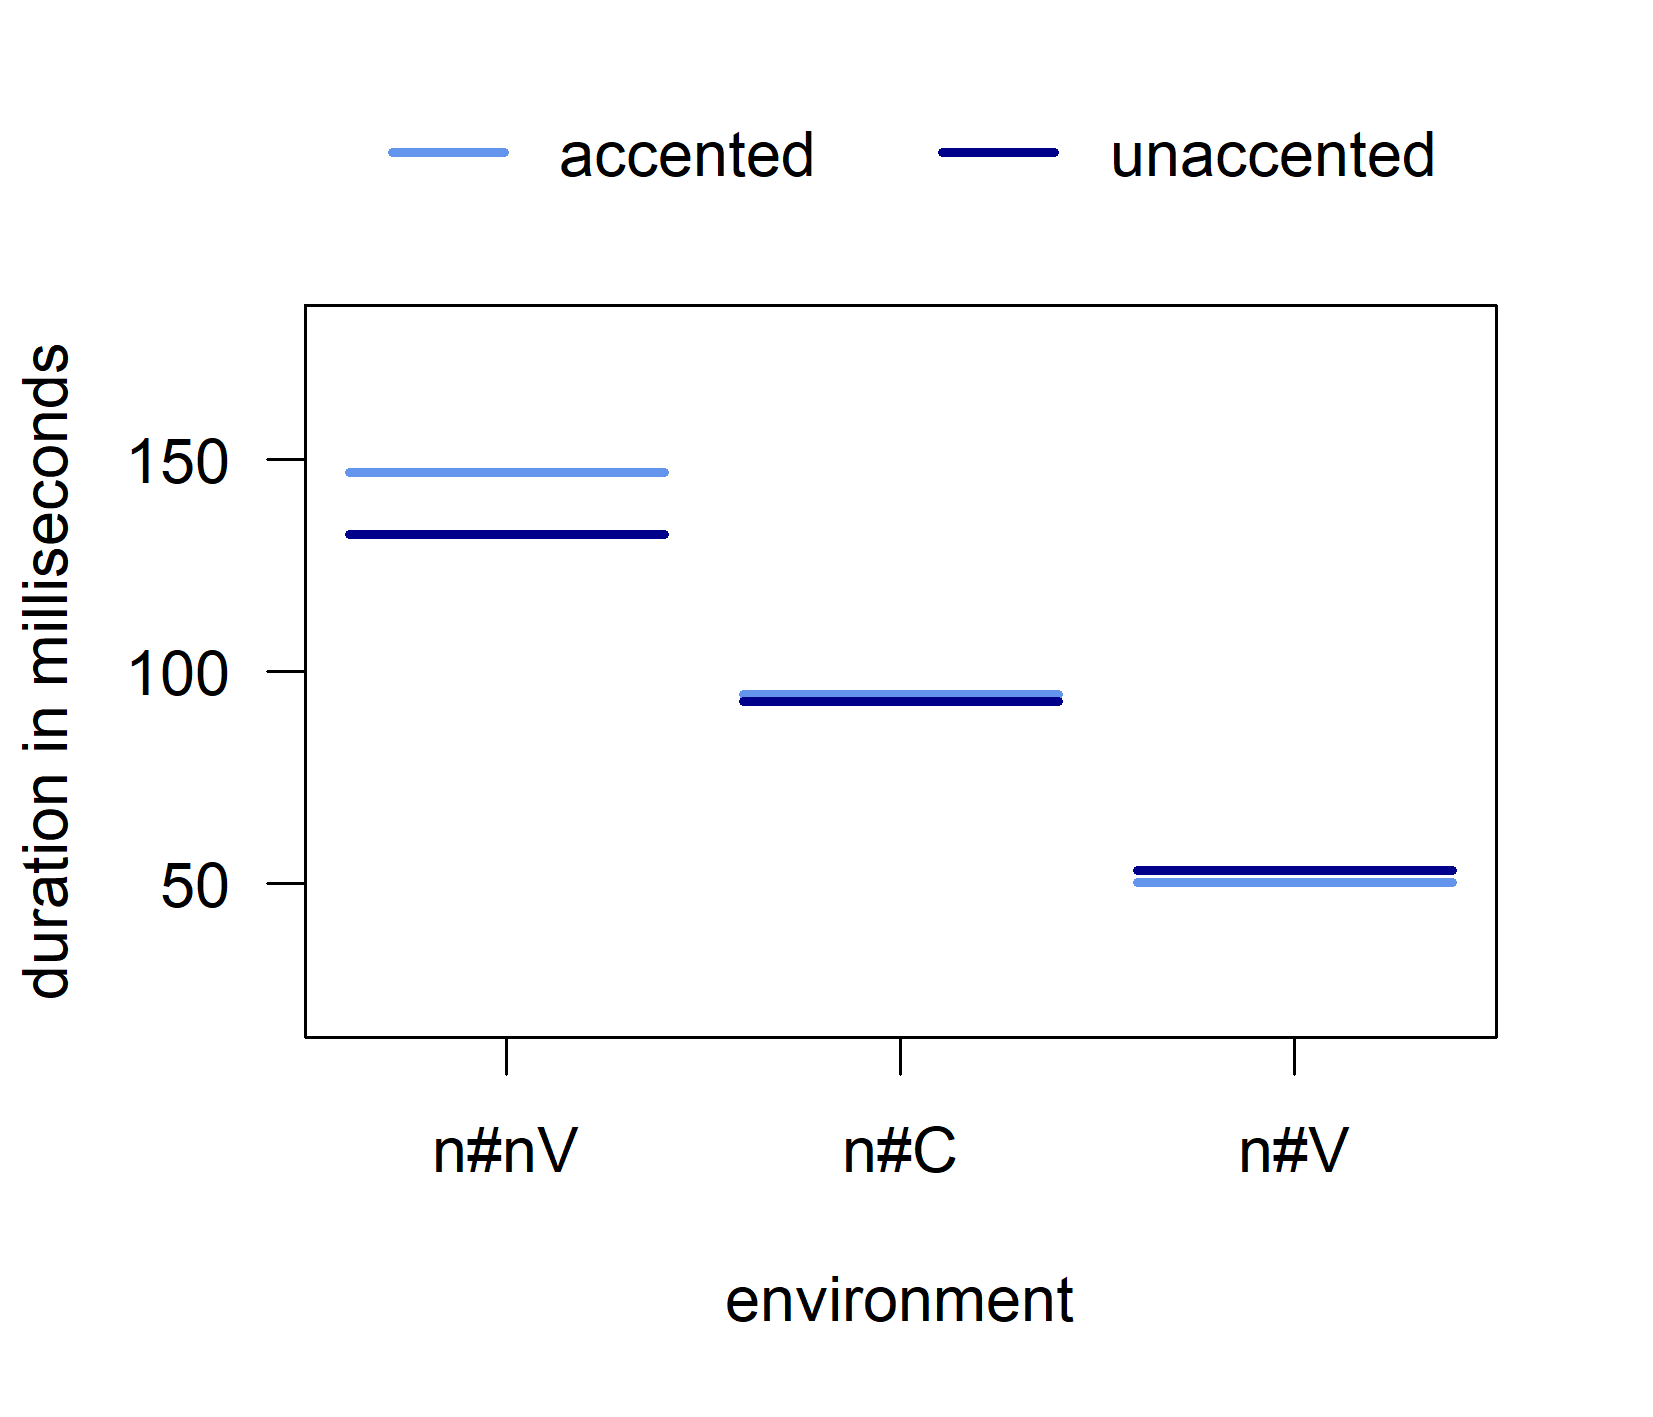
\includegraphics [scale=0.5] {images/Experiment/unModelInterCatAcc}
	\caption{Effect of accentuation by environment on consonant duration in complex \prefix{un}data set}
	\label{fig:NumNasal unComplex experiment}
\end{figure*}


The fourth significant noise variable \textsc{Accentuation} forms an interaction with the variable of interest \textsc{Environment}. The interaction is depicted in \figref{fig:NumNasal unComplex experiment}.
The light blue lines in the figure show the effect of \textsc{Environment} for items in \is{accentuation}accented position, and the dark blue lines show the effect for items in unaccented position. In both conditions, i.e. in the \is{accentuation}accented and in the unaccented condition, there is a significant durational difference between doubles (\texttt{n\#nV}) and singletons (\texttt{n\#C}, \texttt{n\#V}). 
 In \is{accentuation}accented position, doubles are predicted to be 53~ms longer than singletons followed by a consonant, and 97~ms longer than singletons followed by a vowel. 
 In unaccented position, doubles are also predicted to be longer than both types of singletons but the durational differences are smaller. The differences are 39~ms  for singletons followed by a consonant (\texttt{n\#C}), and 80~ms for singletons followed by a vowel (\texttt{n\#V}). The difference between the two singleton levels is roughly the same in both conditions (45~ms in \is{accentuation}accented position, 40~ms in unaccented position).




 The results clearly show that \is{un-}\prefix{un} geminates. Phonological doubles are predicted to be more than twice as long as phonological singletons followed by a vowel, and the predicted singleton-double ratios for consonant adjacent singletons are, depending on \isi{accentuation}, 1:1.4 and 1:1.6. In comparison to former studies, these durational differences are very large (see Sections~\ref{what is gemination} and~\ref{un corpus} for a discussion of durational differences between geminates and their corresponding singletons). 




\begin{figure}
	
	
	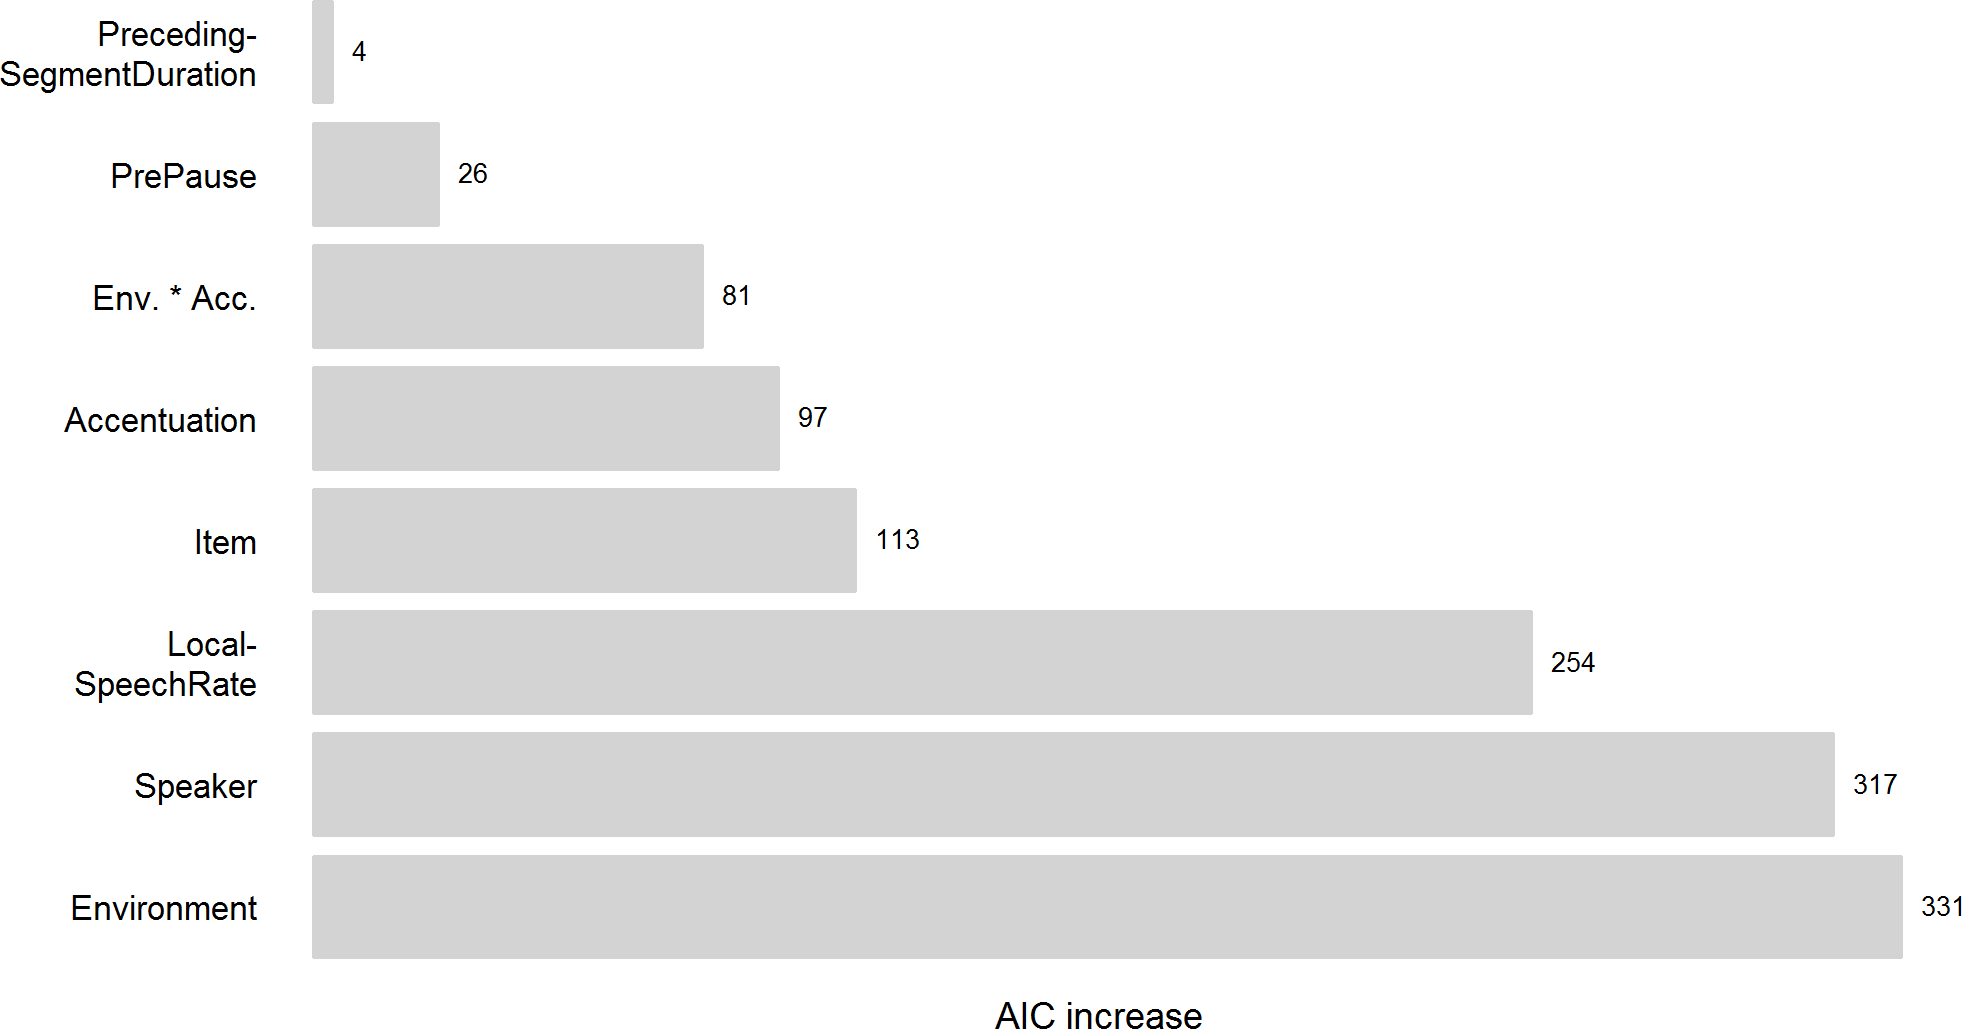
\includegraphics[scale=0.7] {images/Experiment/AICdecreaseUnComplex.png}


	\caption{AIC increase for each variable of the final \prefix{un}model, AIC final model = -11398}
	\label{fig:Effect sozed un Exp unV vs Unn}

\end{figure}



To test the contribution of each variable for the model's goodness of fit, I checked how the absence of each term affects the AIC of the model. \figref{fig:Effect sozed un Exp unV vs Unn} displays the increase of the model's AIC  without each factor. The higher the increase, the more variance is explained by the pertinent factor in the model.



The figure clearly shows that the variable \textsc{Environment} explains most of the variation found in the data. In other words, the absence or presence of a phonological double consonant explains a large portion of the durational differences found in the data.
Furthermore, there are speaker-dependent differences, i.e. different speakers produce the nasal in \is{un-}\prefix{un}prefixed words with different durations. However, it is important to note that while there are overall differences in the duration of the nasal between speakers, all speakers show the same pattern with regard to \isi{gemination}, i.e. all of them produced the double consonants with longer durations than the singletons. 
The third most important variable is \textsc{LocalSpeechRate}. The other noise variables, as well as the interaction, are much less important for the model, i.e. they explain much less of the variance found in the data.


To sum up, the analyses have shown that \is{un-}\prefix{un} clearly geminates, and that the duration of the nasal in \is{un-}\prefix{un}prefixed words is furthermore influenced by phonetic and prosodic factors.
The variables \textsc{Environment} and \textsc{LocalSpeechRate} are two of the most important determiners for consonant duration with \is{un-}\prefix{un}. In addition to \textsc{Speaker}, they explain most of the variance in the data. This result fits in well with the findings of the corpus study, where these two variables were the only two significant predictors for nasal duration with \is{un-}\prefix{un}. 
Furthermore, the two prosodic variables \textsc{Accentuation} and \textsc{PrePause} are rather important predictor variables. The variable \textsc{PrecedingSegmentDuration}, even though significant in the final model, is of less importance. 
%The analyses also indicate that there are item-specific effects which might be related to an item's \isi{stress} pattern and its \isi{frequency}.



\subsubsection{Complete model}

The second \is{un-}\prefix{un}model investigates nasal duration in all tokens of the \is{un-}\prefix{un}data set ($N=2615)$, i.e. it investigates nasal duration in prefixed words and in base words. 
As in the model predicting nasal duration with only complex words, the dependent variable \textsc{AbsoluteConsonantDuration} was Box-Cox-transformed ($\lambda= 0.182$) and outliers ($N=66$, i.e. $ 2.52$\% of the data) were removed to achieve a normal distribution of residuals. The model was then simplified and interactions were tested (see \hyperref[Appendix G Summaries of tested interactions in experimental study]{Appendix G} for a list of all tested interactions). The final model is displayed in \tabref{model un complete experiment} in \hyperref[Appendix H: Model Summaries Experiment]{Appendix H}.


The final model features the variables \textsc{Environment}, \textsc{LocalSpeechRate}, \textsc{BaseInitialStress}, \textsc{Accentuation} and \textsc{PrePause}.
The two noise variables \textsc{Local-SpeechRate} and \textsc{BaseInitialStress} show the expected effects. The faster the \isi{speech rate}, the longer the nasal, and when the base-initial syllable is unstressed the nasal is shorter than when the base-initial syllable is \is{stress}stressed.
The two other noise variables \textsc{Accentuation} and \textsc{PrePause} interact with the variable of interest \textsc{Environment}. Note that there is no three-way interaction between  \textsc{Accentuation}, \textsc{PrePause} and \textsc{Environment}.

\figref{fig:NumNasal Acc un experiment} shows the effect of \textsc{Accentuation} by \textsc{Environment}. The light blue lines represent the estimated durations for words  in \is{accentuation}accented position, the dark blue lines show the estimated durations for words in unaccented position. In both conditions, i.e. in \is{accentuation}accented and unaccented condition, double consonants are predicted to be significantly longer than all types of singletons. This means \is{un-}\prefix{un} geminates, independent of \isi{accentuation}.

\begin{figure*}
	
	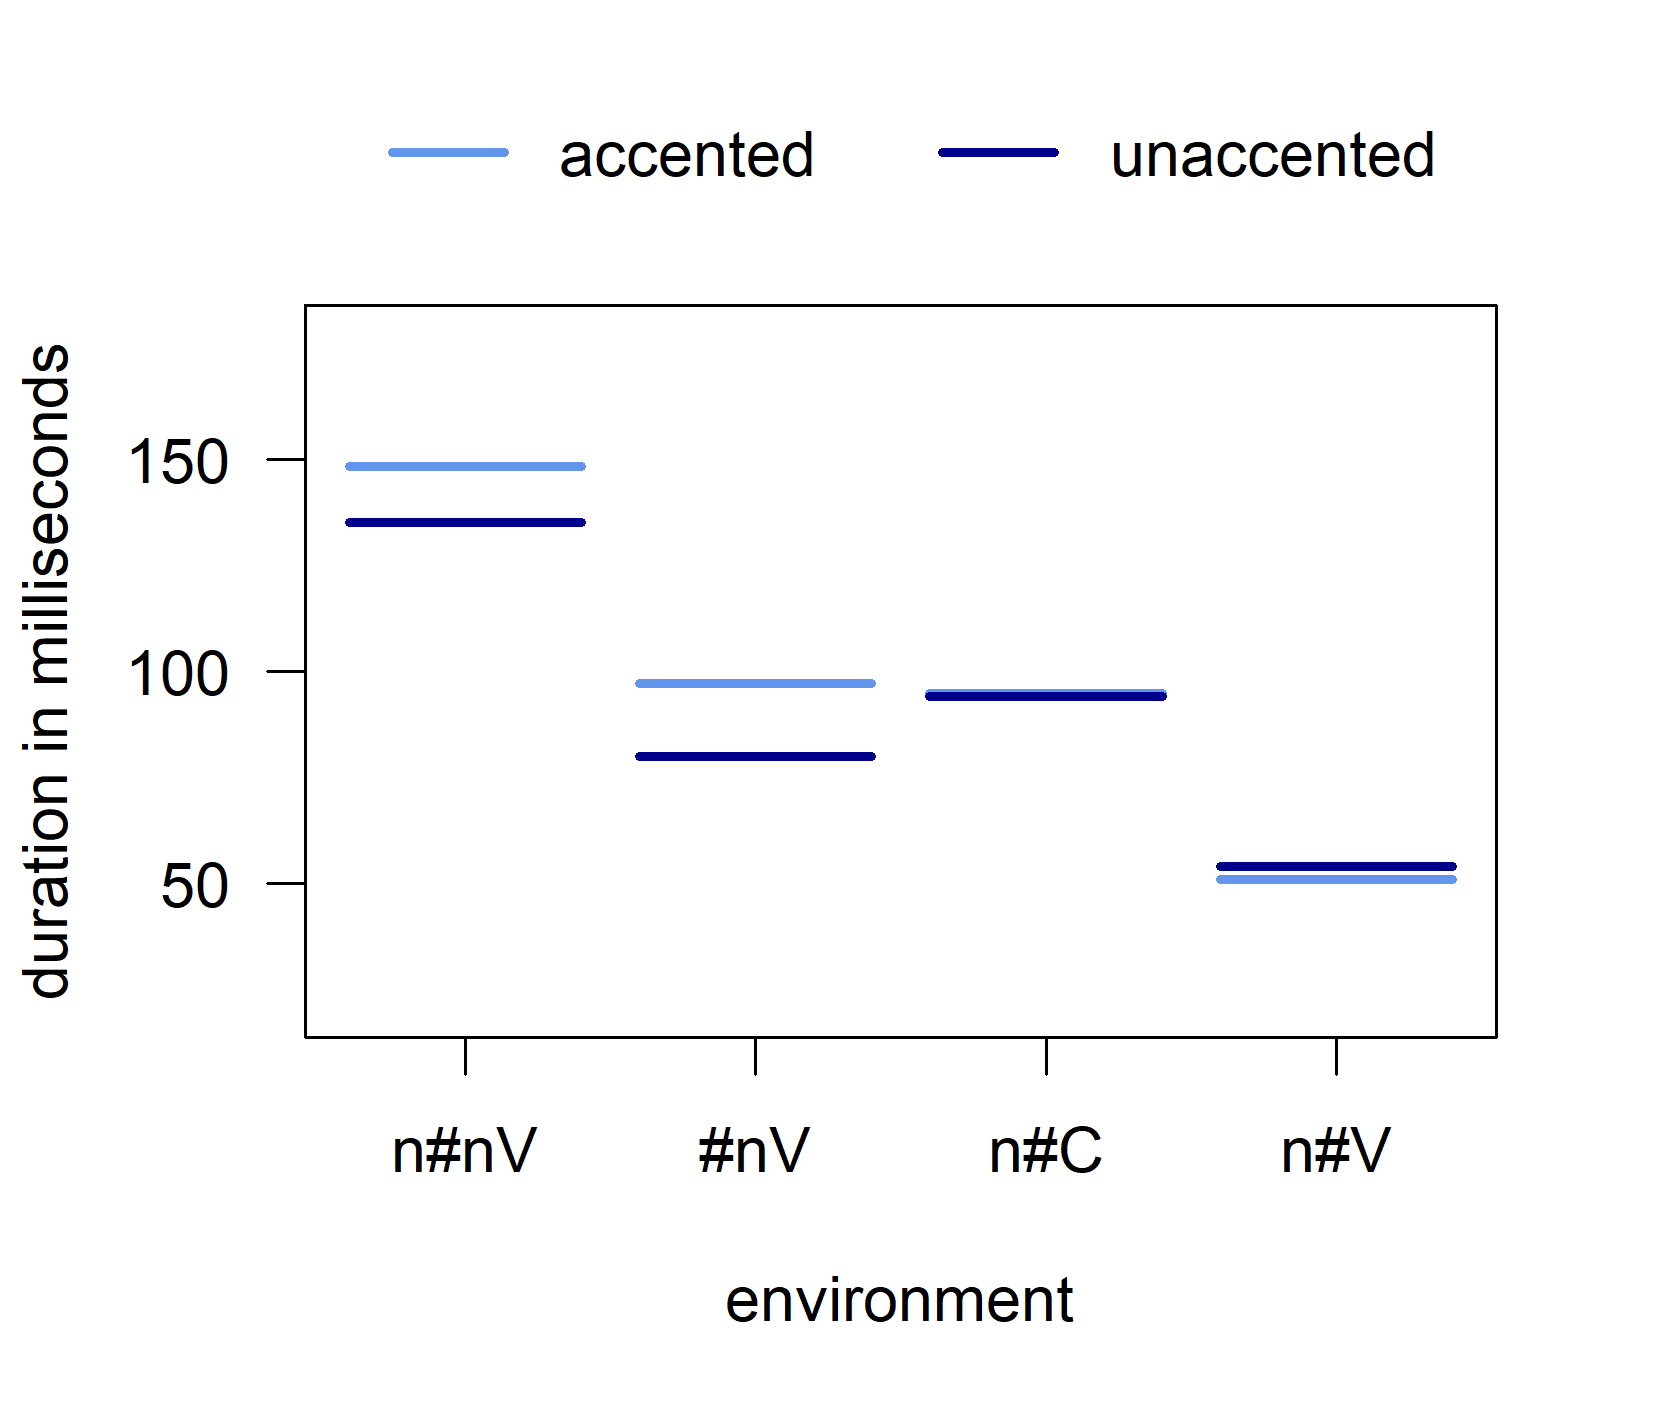
\includegraphics [scale=0.5] {images/Experiment/unModelCompleteInterEnvAcc}
	
	\caption{Effect of accentuation by environment on consonant duration in complete \prefix{un}data set}
	\label{fig:NumNasal Acc un experiment}
\end{figure*}


 For  doubles (\texttt{n\#nV}) and singletons in base words (\texttt{\#nV}), nasals in \is{accentuation}accented words are longer than nasals in unaccented words.
For singletons in complex words (\texttt{n\#C} and \texttt{n\#V}), consonant duration is not affected by \isi{accentuation}. This has the effect that durational differences between doubles and singletons in complex words are bigger in \is{accentuation}accented than in unaccented position. The durational difference between doubles and singletons in base words is not affected by \isi{accentuation}.







\figref{fig:NumNasal Pauseun experiment} shows the effect of \textsc{PrePause} by \textsc{Environment}. The light blue lines represent the estimated durations for words with no preceding pause, the dark blue lines show the estimated durations for words with a preceding pause. 
The figure shows that all doubles are longer than all types of singletons, i.e. \is{un-}\prefix{un} geminates independent of whether a pause precedes a word or not.
As with \textsc{Accentuation}, only the two environments \texttt{n\#nV} and \texttt{\#nV} are affected by the variable \textsc{PrePause}. For items with a double consonants (\texttt{n\#nV}), the nasal is longer when a pause precedes the word. For base words, the opposite is the case, i.e. the nasal is shorter after a preceding pause.
Crucially, \isi{gemination} does not depend on \textsc{PrePause}. 

					\begin{figure*}
	
	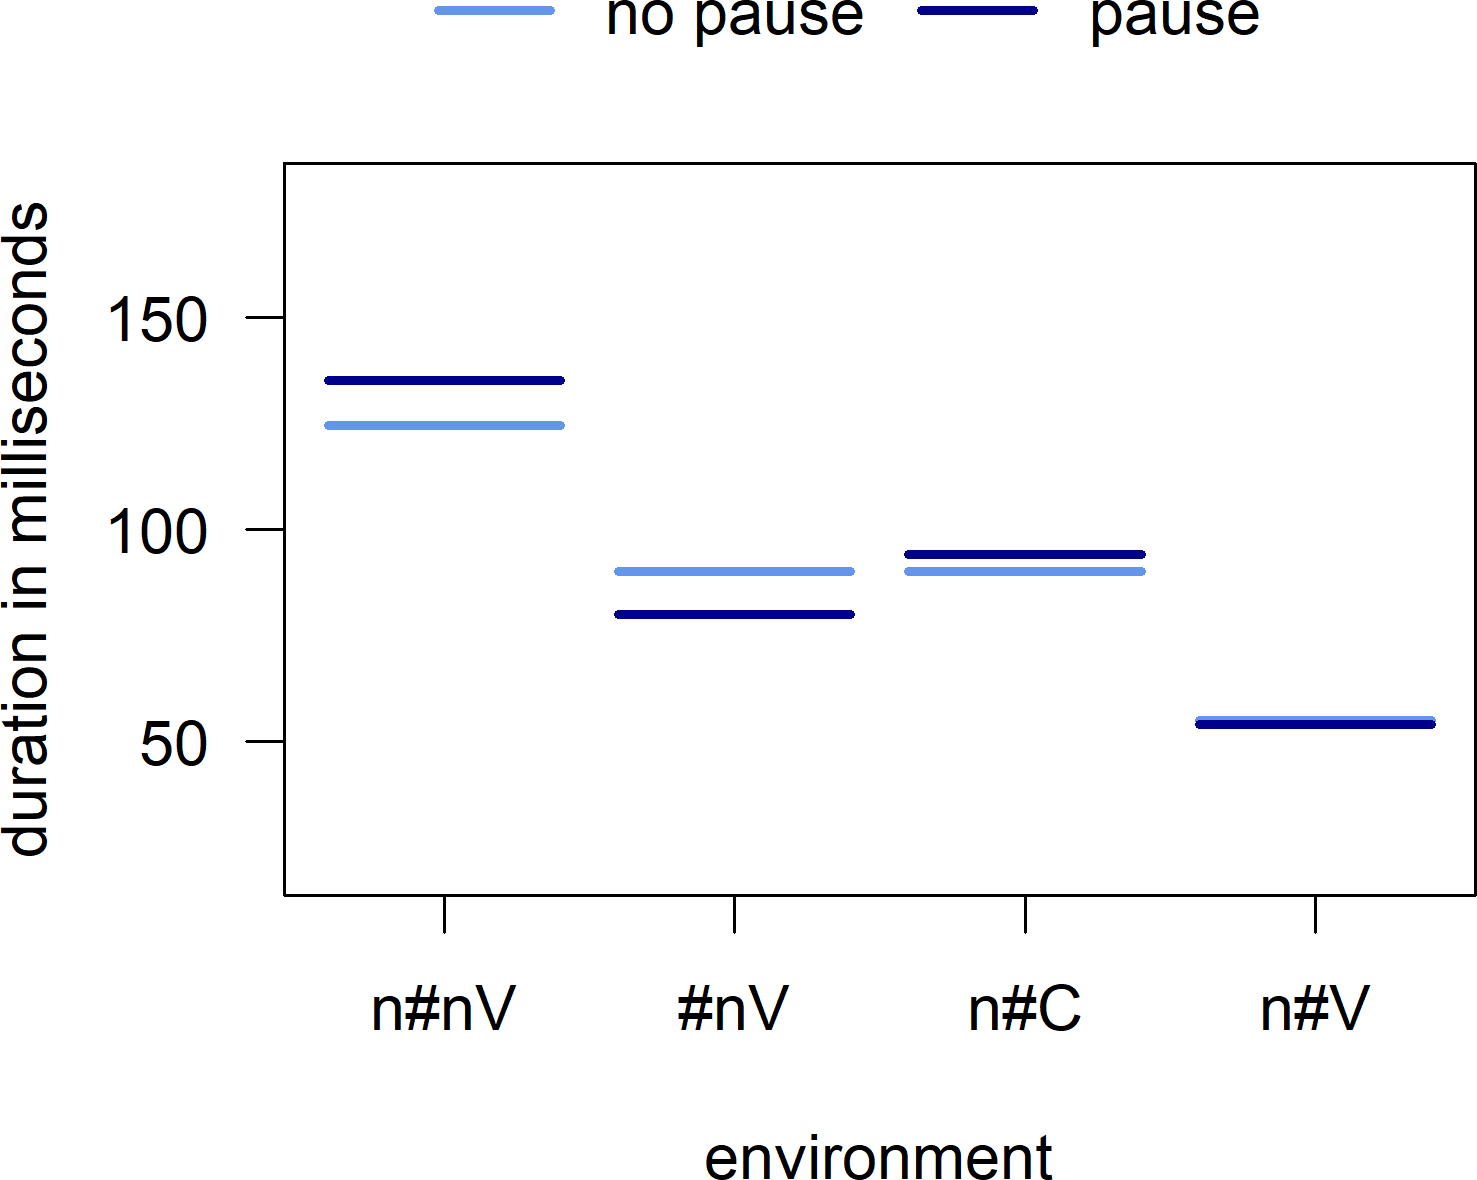
\includegraphics [scale=0.5] {images/Experiment/unModelCompleteInterEnvPause}
	\caption{Effect of pause before item by environment on consonant duration in complete \prefix{un}data set}
	\label{fig:NumNasal Pauseun experiment}
\end{figure*}
%



\subsubsection{Summary}


The prefix \is{un-}\prefix{un} clearly geminates. Phonological doubles (\texttt{n\#nV})  are longer than singletons in complex words (\texttt{n\#C}, \texttt{n\#V}) and singletons in base words (\texttt{\#nV}). There are also significant durational differences between the singleton levels with the singletons in base words being the longest, the singletons in prefixed words followed by a consonant being the second longest and the singletons in prefixed words followed by a vowel being the shortest. This pattern resembles the one found in the corpus study. The durational differences between doubles and singletons are, however, much bigger in the experimental study than in the corpus study, i.e. \isi{gemination} seems to be more extreme in the experimental data than in the corpus data. 
As in the corpus study, the \isi{decomposability} measure log\textsc{RelativeFrequency} does not affect nasal duration with \is{un-}\prefix{un}.


 In both \is{un-}\prefix{un}models, the noise variables show the expected effects. In the complex model, the noise variables \textsc{Accentuation}, \textsc{LocalSpeechRate}, \textsc{PrePause} and \textsc{PrecedingSegmentDuration} proved to be significant. In the complete mo-del, the noise variables \textsc{Accentuation}, \textsc{LocalSpeechRate}, \textsc{PrePause} and \textsc{BaseInitialStress} proved to be significant.
 The noise variable \textsc{Accentuation} interacts with the variable \textsc{Environment} in both models. While doubles and singletons in base words are longer when \is{accentuation}accented, singletons in base words are not. In the complete model, there is an interaction between \textsc{PrePause} and \textsc{Environment}. Again, only doubles and singletons in base words are affected by this variable. Crucially,  whether \is{un-}\prefix{un} geminates or not does not depend on \isi{accentuation} or a preceding pause. 


\subsection{The prefix \textit{in-}} \label{in experiment}

\subsubsection{The allomorph /ɪn/: Complex model}

The model predicting consonant duration with all complex /ɪn/-words ($N=1232$) was fitted according to the modeling procedure described in \sectref{stats}. Due to an uneven distribution of the residuals in the initial model, the dependent variable \textsc{AbsoluteConsonantDuration} was Box-Cox-transformed ($\lambda = 0.061$) and 22 outliers were removed (1.9\% of the data).
After the model was refitted with the transformed dependent variable, it showed a satisfactory distribution of residuals.  The model was then simplified and interactions were tested (see \hyperref[Appendix G Summaries of tested interactions in experimental study]{Appendix G} for a list of all tested interactions).
The \is{decomposability measure}decomposability variables were tested individually.

The final model features five variables, \textsc{Environment}, \textsc{BaseInitialStress}, \textsc{Accentuation}, \textsc{LocalSpeechRate} and \textsc{PrecedingSegmentDuration}. 
There are two interactions in the model, one between \textsc{Environment} and \textsc{BaseInitialStress}, and one between \textsc{Environment} and \textsc{Accentuation}. The final model is summarized in \tabref{model in complex experiment} in \hyperref[Appendix H: Model Summaries Experiment]{Appendix H}.


The two noise variables \textsc{LocalSpeechRate} and \textsc{PrecedingSegmentDuration} behave as expected. The higher the \isi{speech rate}, the shorter the consonant, and the longer the preceding segment, the shorter the nasal. 


\figref{fig:Env Stress In experiment} shows the interaction between \textsc{BaseInitialStress} and \textsc{Environment}. For each environment, the estimated consonant durations for words with a \is{stress}stressed base-initial syllable are indicated by light blue lines, and the estimated durations for words with an unstressed base-initial syllable are indicated by dark blue lines. 
The plot shows that only when the base-initial syllable of a word is \is{stress}stressed, doubles are predicted to be clearly longer than singletons followed by a vowel (33~ms). When the base-initial syllable of a word is unstressed, doubles (\texttt{n\#nV}) are predicted to be only 10~ms longer than singletons followed by a vowel (\texttt{n\#V}).
Doubles are never predicted to be longer than singletons followed by a consonant  (\texttt{n\#C}).
When the base-initial syllable of a word is \is{stress}stressed, doubles are predicted to be as long as singletons followed by a consonant (\texttt{n\#C}). When the base-initial syllable of a word is unstressed, doubles are predicted to be 41~ms shorter than singletons followed by a consonant (\texttt{n\#C}).




 	\begin{figure*}

 		
 		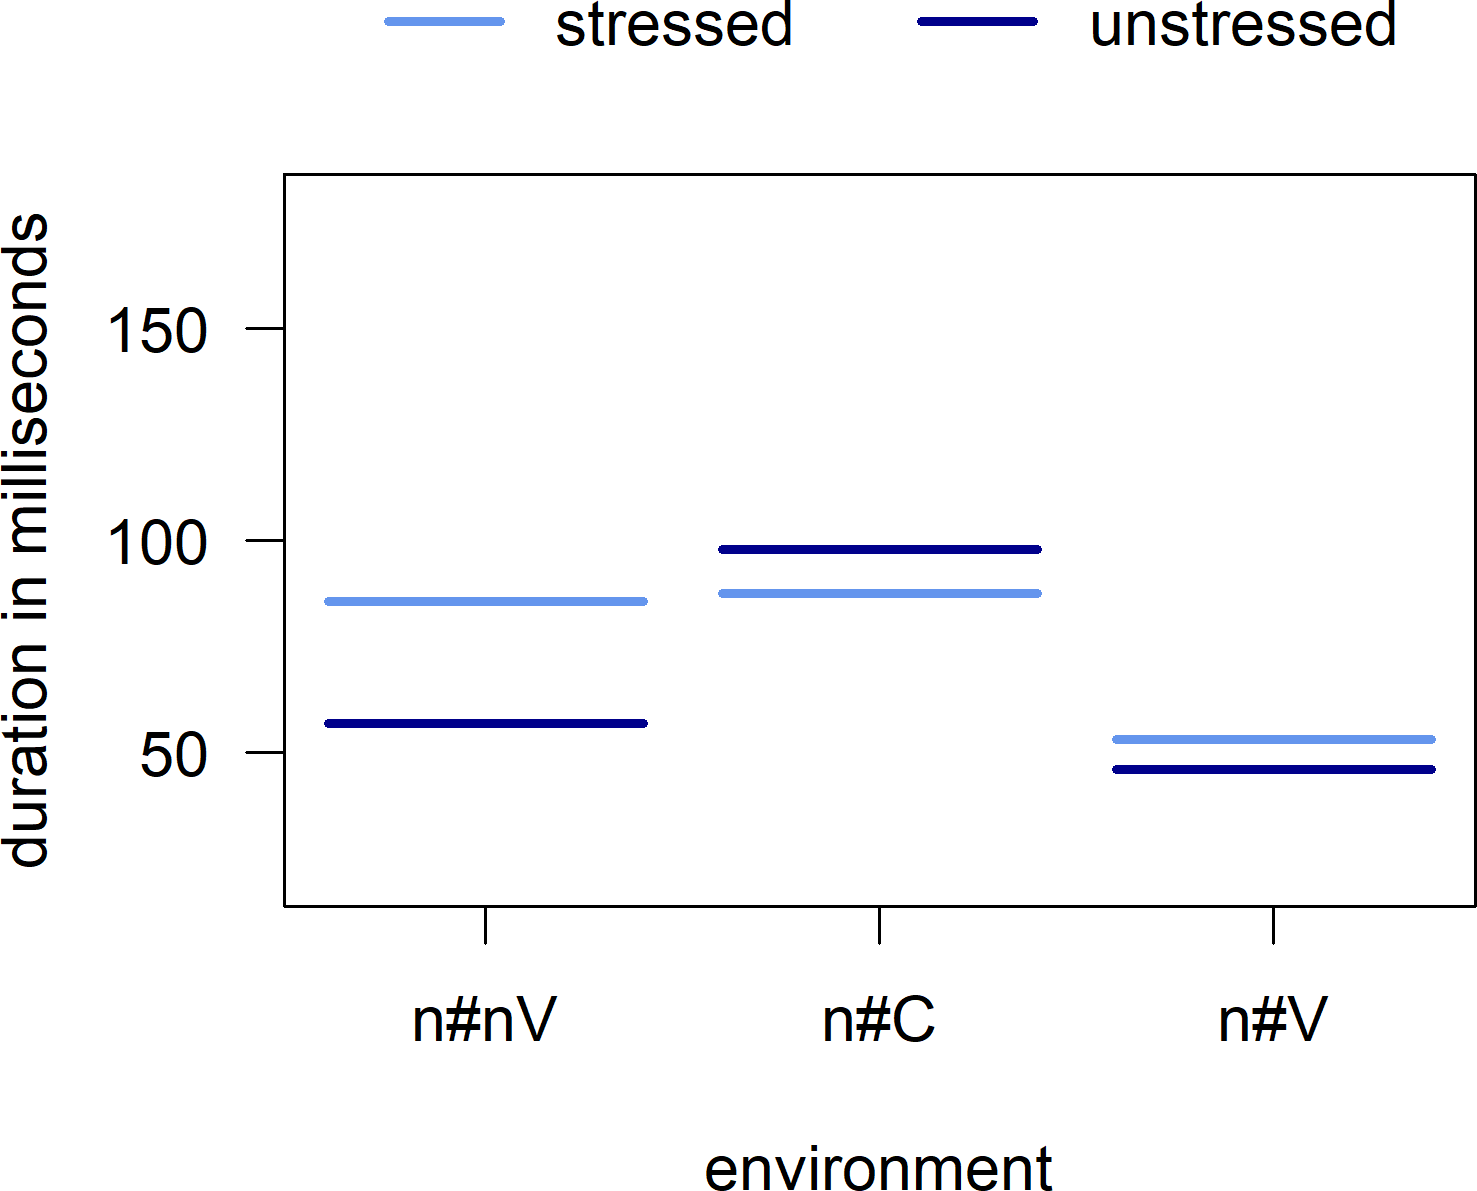
\includegraphics [scale=0.5] {images/Experiment/InModelInterEnvStress}
		
 		\caption{Effect of base-initial stress by environment on consonant duration in complex /ɪn/-data set}		
 		\label{fig:Env Stress In experiment}

 	\end{figure*}%
 	
 	
 

\figref{fig:Env Acc In experiment} shows the interaction between \textsc{Accentuation} and \textsc{Environment}. Light blue lines represent the estimates for \is{accentuation}accented items, and dark blue lines represent the estimated for unaccented items. Note that the figure shows the estimates for items with an unstressed base-initial syllable, and that there is no three-way-interaction between \textsc{BaseInitialStress}, \textsc{Accentuation} and \textsc{Environment}. 


	


	\begin{figure*} 
		
		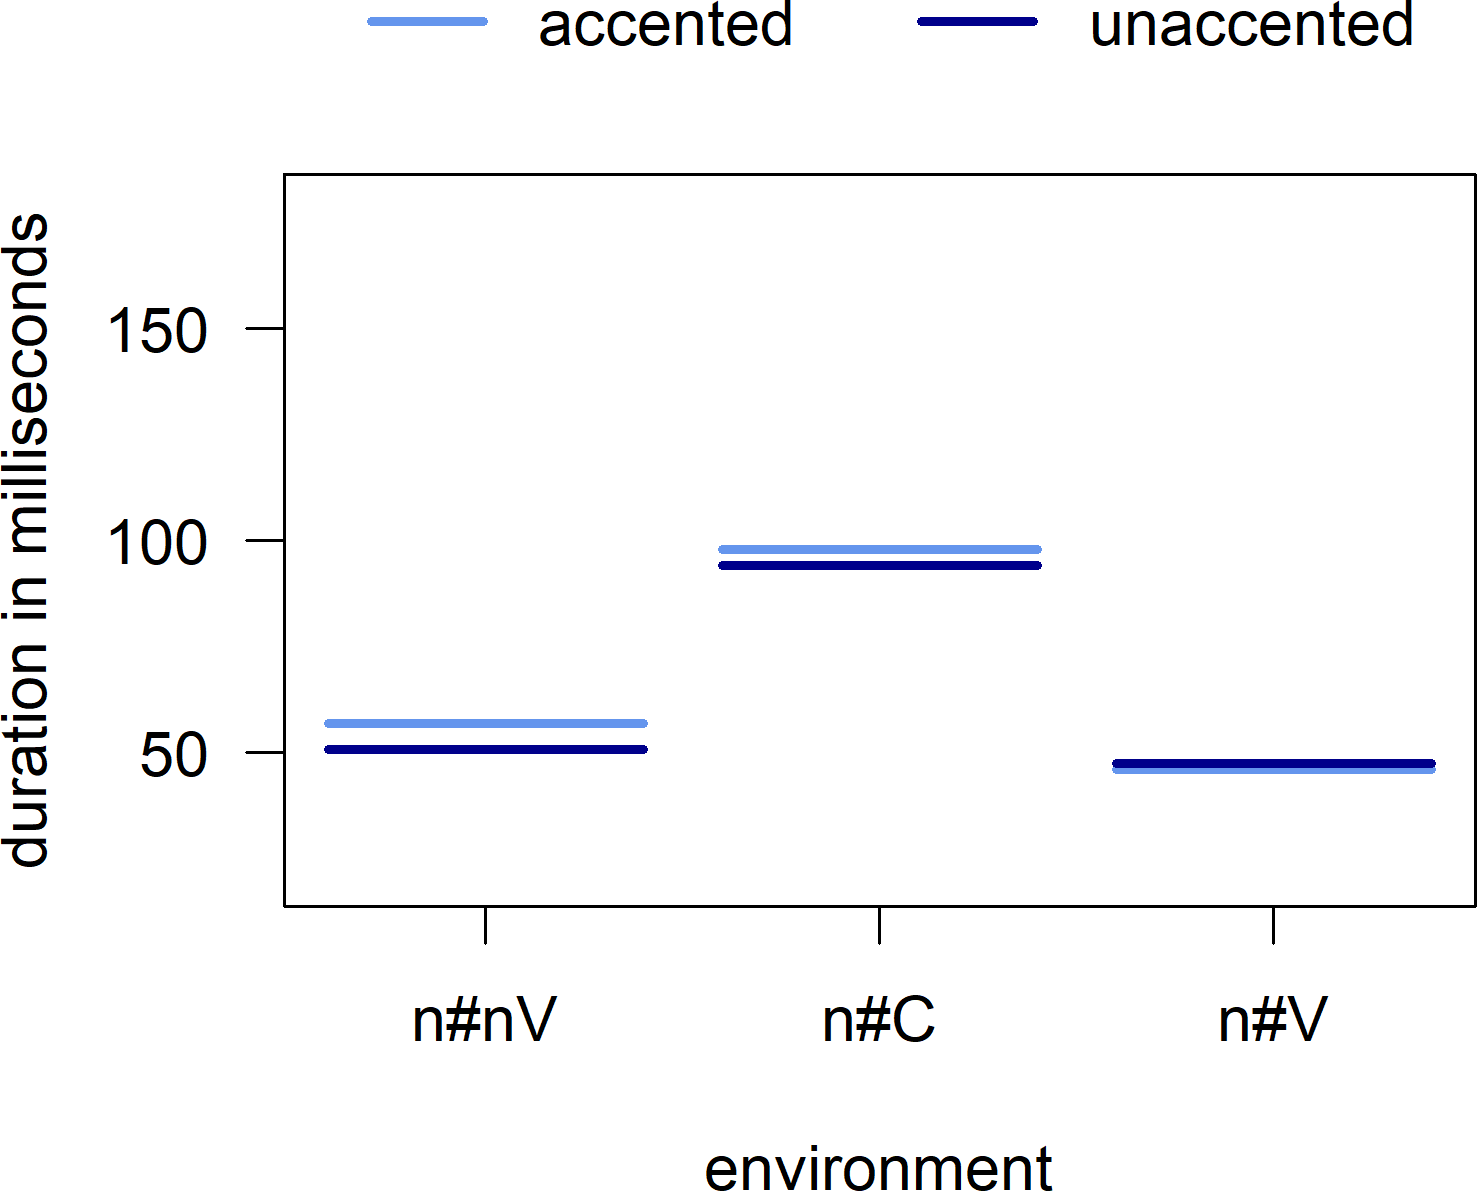
\includegraphics [scale=0.5] {images/Experiment/InModelInterEnvAcc}
		%\vspace*{-0.2cm}
		\caption{Effect of accentuation by environment on consonant duration in complex /ɪn/-data set}
		\label{fig:Env Acc In experiment} 
	\end{figure*}






The figure shows that while double consonants (\texttt{n\#nV}) and singletons followed by a consonant (\texttt{n\#C}) are slightly longer when the word is \is{accentuation}accented, singletons followed by a vowel (\texttt{n\#V}) are not affected by \textsc{Accentuation}. Crucially, 
the durational pattern of the three environments does not change depending on whether a word is \is{accentuation}accented or unaccented. 
With unstressed base-initial syllables, singletons followed by a consonant (\texttt{n\#C}) are the longest, followed by doubles (\texttt{n\#nV}), and singletons followed by a vowel (\texttt{n\#V}) are the shortest.
With \is{stress}stressed base-initial syllables, doubles (\texttt{n\#nV}) and singletons followed by a consonant (\texttt{n\#C}) are of the same duration, and singletons followed by a vowel (\texttt{n\#V}) are shorter.\footnote{Note that the durational differences for words with \is{stress}stressed base-initial syllables cannot be seen in \figref{fig:Env Acc In experiment}.}


%AIC

The effect size of each significant term in the model is displayed in \figref{fig:Effect sizes InComplex Exp}. As in the \is{un-}\prefix{un}model, the variables \textsc{Speaker}, \textsc{Environment}, \textsc{LocalSpeechRate} and \textsc{Item} explain most of the variance found in the data. Crucially, the variable \textsc{Environment} is very important for the model, i.e. the number of consonants at the morphological boundary, as well as the segment following the nasal, highly influence the duration of the nasal. In contrast to \is{un-}\prefix{un}, \textsc{Environment} does, however, not explain most of the variance found in the data. It thus seems that it is less important for predicting consonant duration with /ɪn/-prefixed words than with \is{un-}\prefix{un}prefixed words. 





%PC Model

None of the \is{decomposability measure}decomposability measures proved to be significant in the final model. On the one hand, this might mean that \isi{decomposability} does not affect consonant duration with /ɪn/. On the other, there is the possibility that the individual \is{decomposability measure}decomposability measures are not strong enough to reach significance on their own. As a combined \isi{decomposability} measure, they might, however, become significant in the model (see also discussions in Sections~\ref{analsyses duration experiment} and~\ref{in corpus}).





\begin{figure*}
	
	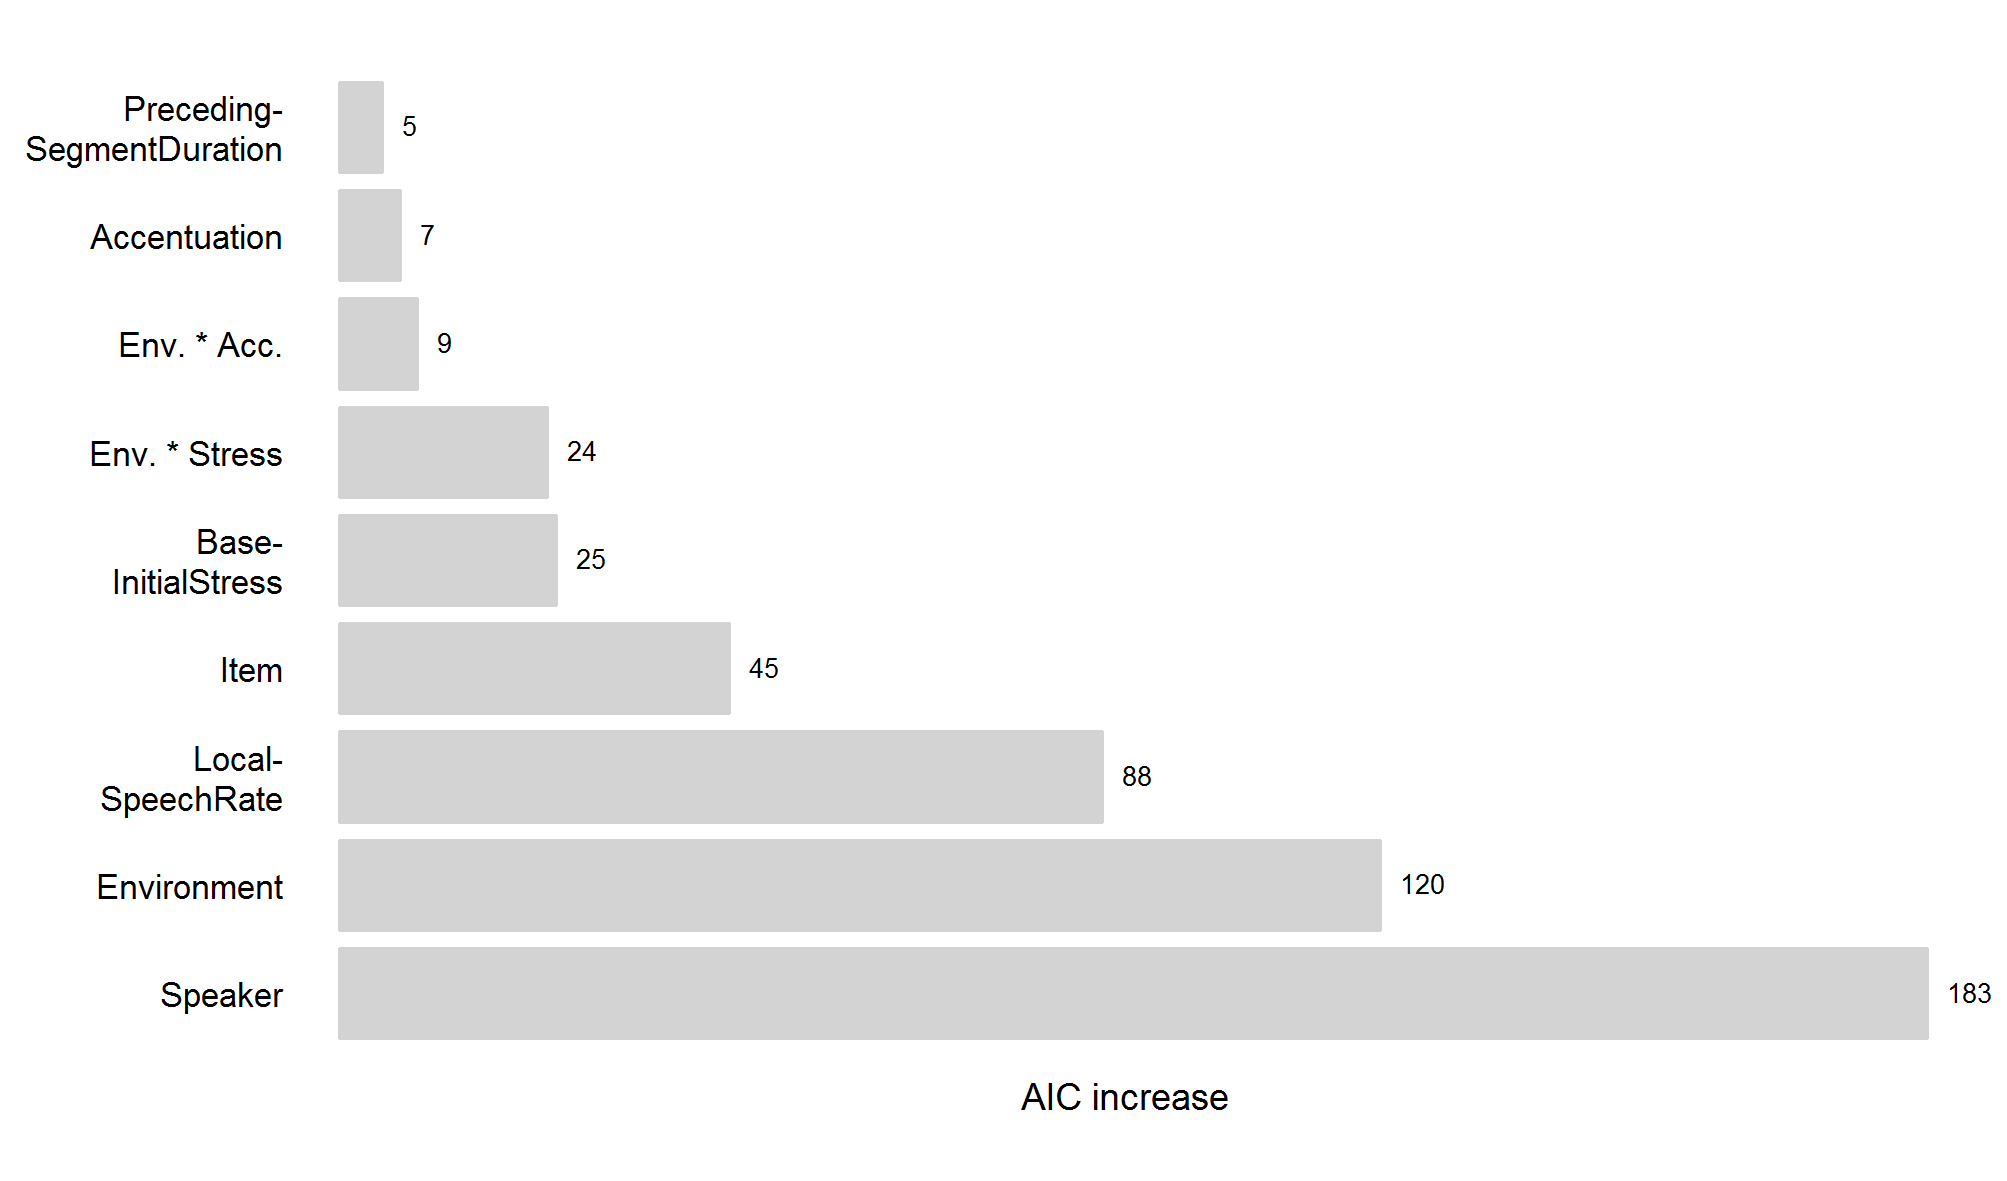
\includegraphics[scale=0.7]{images/Experiment/AICdecreaseInComplex.png}
	
	\caption{AIC increase for each variable of the final /ɪn/-model, AIC final model = -6974}
	\label{fig:Effect sizes InComplex Exp}
	
\end{figure*}


To test this idea, an additional model with combined \is{decomposability measure}decomposability measures (as opposed to individual \is{decomposability measure}decomposability measures) was fitted. The combined measures were created by means of a \is{principal component analysis}principal component analysis (see \sectref{stats} on \is{principal component analysis}principal component analyses). 
As in the corpus study, the \is{principal component analysis}principal component analysis was fitted with the variables log\textsc{RelativeFrequency}, \textsc{SemanticTransparency}, \textsc{SemanticTransparencyRating}, \textsc{TypeOfBase} and \textsc{Affix}. The variable \textsc{Affix} features the two levels \texttt{inLoc} (\is{locative in-}locative \prefix{in}) and \texttt{inNeg} (\is{negative in-}negative \prefix{in}). All variables were recoded into numerical variables and scaled before the analysis was conducted. 
\tabref{tbl: summary PC in exp} summarizes the analysis by showing the composition of each \is{principal component analysis}principal component, i.e. the loading of each variable for each \is{principal component analysis}principal component, and by displaying the proportion of variance covered by each component. 










The \is{principal component analysis}principal component analysis revealed that the first three components can account for most of the variance expressed by the five \is{decomposability measure}decomposability variables (90\%). An inspection of the rotation matrix shows that the first component is composed of all five measures, that the second is mainly dominated by the variables scaled\textsc{Affix} and scaled\textsc{RelativeFrequency}, and that the third is mainly dominated by the variable scaled\textsc{SemanticTransparencyRating}. 
The first three principal components were included as predictor variables in the mixed model.  




\begin{table*}
	\caption{Summary of principal components\label{tbl: summary PC in exp}}
	\resizebox{\textwidth}{!}{%		
		\begin{tabular}{l *{5}{S[table-format=+1.3]}}
			\lsptoprule
			 &  {PC1} &   {PC2} &  {PC3} & {PC4} & {PC5}  \\
			\midrule
			\multicolumn{6}{l}{Composition of principal components}\\
			\midrule
				scaled\textsc{Affix} & -0.457 & 0.591 & 0.022 & -0.324 & -0.580 \\
				scaled\textsc{RelativeFrequency}  &  -0.390 & -0.724 & -0.347 & -0.391 & -0.225 \\ 
				scaled\textsc{SemanticTransparencyRating}  &-0.391 & -0.252 & 0.882 & 0.036 & 0.065 \\ 
				scaled\textsc{TypeOfBase}& -0.469 & -0.037 & -0.242 & 0.836 & -0.145 \\ 
				scaled\textsc{SemanticTransparency} & -0.516 & 0.250 & -0.206 & -0.205 & 0.767 \\ 		
			\midrule
			\multicolumn{6}{l}{Variance explained by principal components}\\
			\midrule
				Proportion of Variance &0.626& 0.150& 0.121 & 0.076& 0.027\\
				\lspbottomrule
			\end{tabular}}
\end{table*}

The model was fitted similarly to the model with the individual \is{decomposability measure}decomposability measures. After model simplification, none of the principal components remained in the model. This means, the simplification of the model resulted in the same final model as the simplification of the model with the individual \is{decomposability measure}decomposability measures. Decomposability does not affect consonant duration with /ɪn/.




To sum up, the analyses have shown that prefixal nasal duration in /ɪn/- prefixed words is influenced by the variables \textsc{Environment}, \textsc{BaseInitialStress}, \textsc{Accentuation}, \textsc{LocalSpeechRate} and \textsc{PrecedingSegmentDuration}. None of the \is{decomposability measure}decomposability variables influences nasal duration with /ɪn/, neither as independent measures nor as combined measures. 
While the noise variables \textsc{Accentuation}, \textsc{LocalSpeechRate} and \textsc{PrecedingSegmentDuration} behave as expected and do not influence the \isi{gemination} pattern of /ɪn/, the variable \textsc{BaseInitialStress} affects \isi{gemination} with /ɪn/. 
Only when the base-initial syllable of a prefixed word is \is{stress}stressed, double consonants (\texttt{n\#nV}) are predicted to be clearly longer than singletons with a following vowel (\texttt{n\#V}). In this case, i.e. when the base-initial syllable is \is{stress}stressed, doubles are predicted to be as long as singletons followed by a consonant (\texttt{n\#C}). When the base-initial syllable of a word is unstressed, doubles (\texttt{n\#nV} ) are predicted to be only marginally longer than singletons with a following vowel (\texttt{n\#V}). In this case, they are predicted to be shorter than singletons followed by a consonant (\texttt{n\#C}).

\subsubsection{The allomorph /ɪn/: Complete model}


The model predicting consonant duration with all /ɪn/-words ($N=1232$) was fitted according to the modeling procedure described in \sectref{stats}. Due to an uneven distribution of the residuals in the initial model, the dependent variable \textsc{AbsoluteConsonantDuration} was Box-Cox-transformed ($\lambda = 0.202$) and 22 outliers were removed (1.79\% of the data). 
After the transformation, the model showed a satisfactory distribution of residuals. The model was then simplified and interactions were tested (see \hyperref[Appendix G Summaries of tested interactions in experimental study]{Appendix G} for a list of all tested interactions).




The final model features the five variables \textsc{LocalSpeechRate}, \textsc{Environment}, \textsc{BaseInitialStress}, \textsc{Accentuation} and \textsc{PrePause} (see \tabref{model in complete experiment} in \hyperref[Appendix H: Model Summaries Experiment]{Appendix H} for a summary of the final complete model). 
The noise variable \textsc{LocalSpeechRate} shows the expected effect. The other three noise variables interact with the variable \textsc{Environment}, i.e. there are three two-way interactions in the model, one between \textsc{BaseInitialStress} and \textsc{Environment}, one between \textsc{Accentuation} and \textsc{Environment}, and one between \textsc{PrePause} and \textsc{Environment}.  Note that all pertinent three-way interactions were tested but none proved to be significant.


	\begin{figure*}
		 
		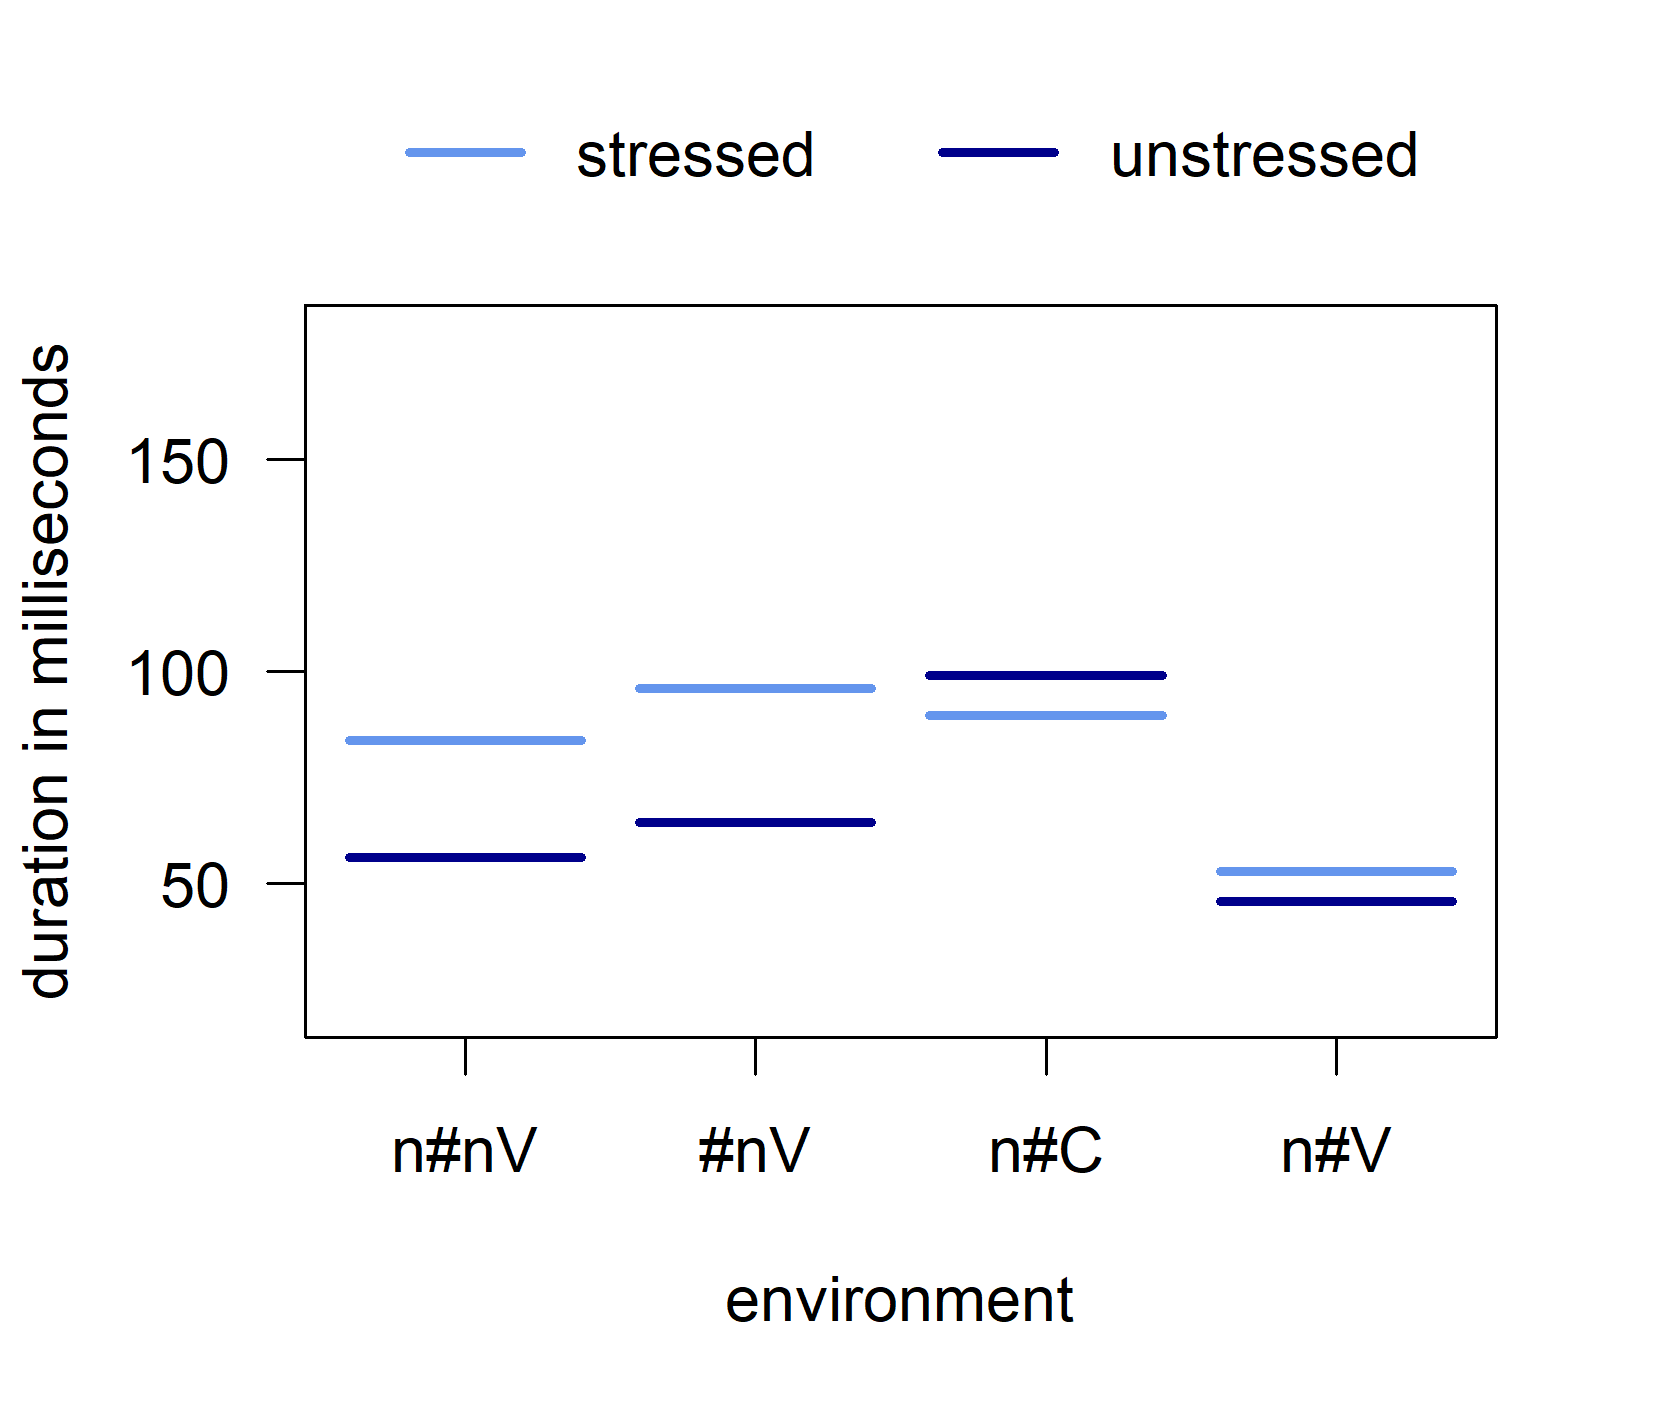
\includegraphics [scale=0.5] {images/Experiment/InModelCompleteInterEnvStress}
		
		\caption{Effect of base-initial stress by environment on consonant duration in /ɪn/-data set}	
		\label{fig:Env Stress In complete experiment} 
	\end{figure*}%








%\isi{stress}
\figref{fig:Env Stress In complete experiment} shows the effect of \textsc{BaseInitialStress} on \textsc{Environment}. Light blue lines indicate estimates for words with \is{stress}stressed base-initial syllables, and dark blue lines indicate estimates for words with unstressed base-initial syllables. The plot shows the predicted durations for \is{accentuation}accented items.



As the complex /ɪn/-model, the complete model reveals that \isi{stress} affects \isi{gemination} with /ɪn/. 
The plot shows that only when doubles (\texttt{n\#nV}) are part of a word with a \is{stress}stressed base-initial syllable, they are as long as singletons with a following consonant  (\texttt{n\#C}) and longer than singletons with a following vowel  (\texttt{n\#V}). When part of a word with an unstressed base-initial syllable, doubles are shorter than singletons followed by a consonant and only slightly longer than singletons followed by a vowel. Independent of \textsc{BaseInitialStress}, doubles are slightly shorter than singletons in base words.




%Acentuation
\figref{fig:Env Acc In complete experiment} shows the interaction between \textsc{Accentuation} and \textsc{Environment}. Estimates for \is{accentuation}accented items are indicated by light blue lines, estimates for unaccented items by dark blue lines. The figure shows the estimates for words with an unstressed base-initial syllable. 


	\begin{figure*}
		
		
		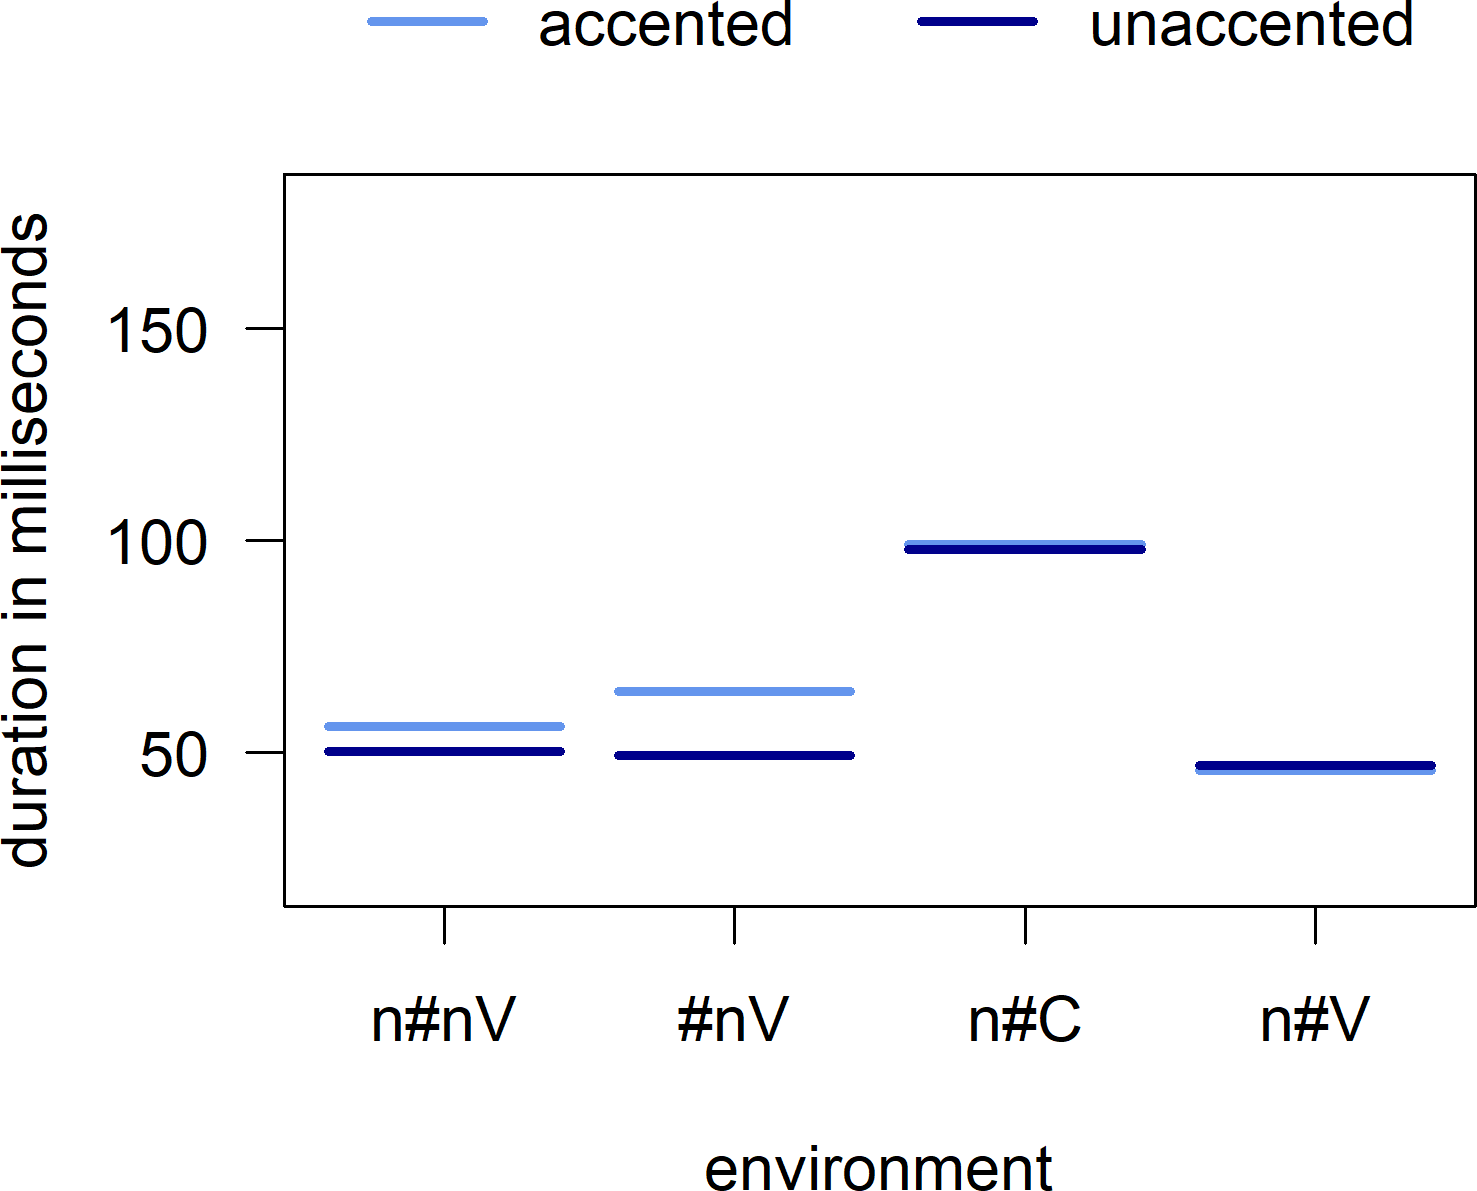
\includegraphics [scale=0.5] {images/Experiment/InModelCompleteInterEnvAcc} 
		\caption{Effect of accentuation by environment on consonant duration in /ɪn/-data set}
		\label{fig:Env Acc In complete experiment}
	\end{figure*}


The plot shows that only the durational pattern of doubles and singletons in base words is affected by \isi{accentuation}. 
In unaccented condition, singletons in base words and doubles are of the same duration. In \is{accentuation}accented condition, singletons in base words are longer. Crucially, doubles are never longer than singletons in base words.
The durational pattern of doubles and singletons in complex words is not affected by \isi{accentuation}. For words with an unstressed base-initial syllable, doubles are shorter than singletons followed by a consonant, and slightly longer than singletons followed by a vowel. For words with a \is{stress}stressed base-initial syllable, doubles are as long as singletons followed by a consonant and longer than singletons followed by a vowel.\footnote{Note that the durational differences for words with \is{stress}stressed base-initial syllables cannot be seen in \figref{fig:Env Acc In complete experiment}.} 


%PrePause

\figref{fig:Env Pause In complete experiment} shows the interaction between \textsc{PrePause} and \textsc{Environment}. Light blue lines indicate the estimated nasal durations for words with no preceding pause, and dark blue lines show the estimated nasal durations for words with a preceding pause.
The figure shows that only the duration of singletons in base words (\texttt{\#nV}) is affected by a preceding pause. When a pause precedes a base word, nasals are shorter than when there is no preceding pause. This effect was also observed with \is{un-}\prefix{un}, and is therefore not surprising. 
The effect of \textsc{PrePause} does not affect \isi{gemination} with /ɪn/.



\begin{figure*}
	
	
	
	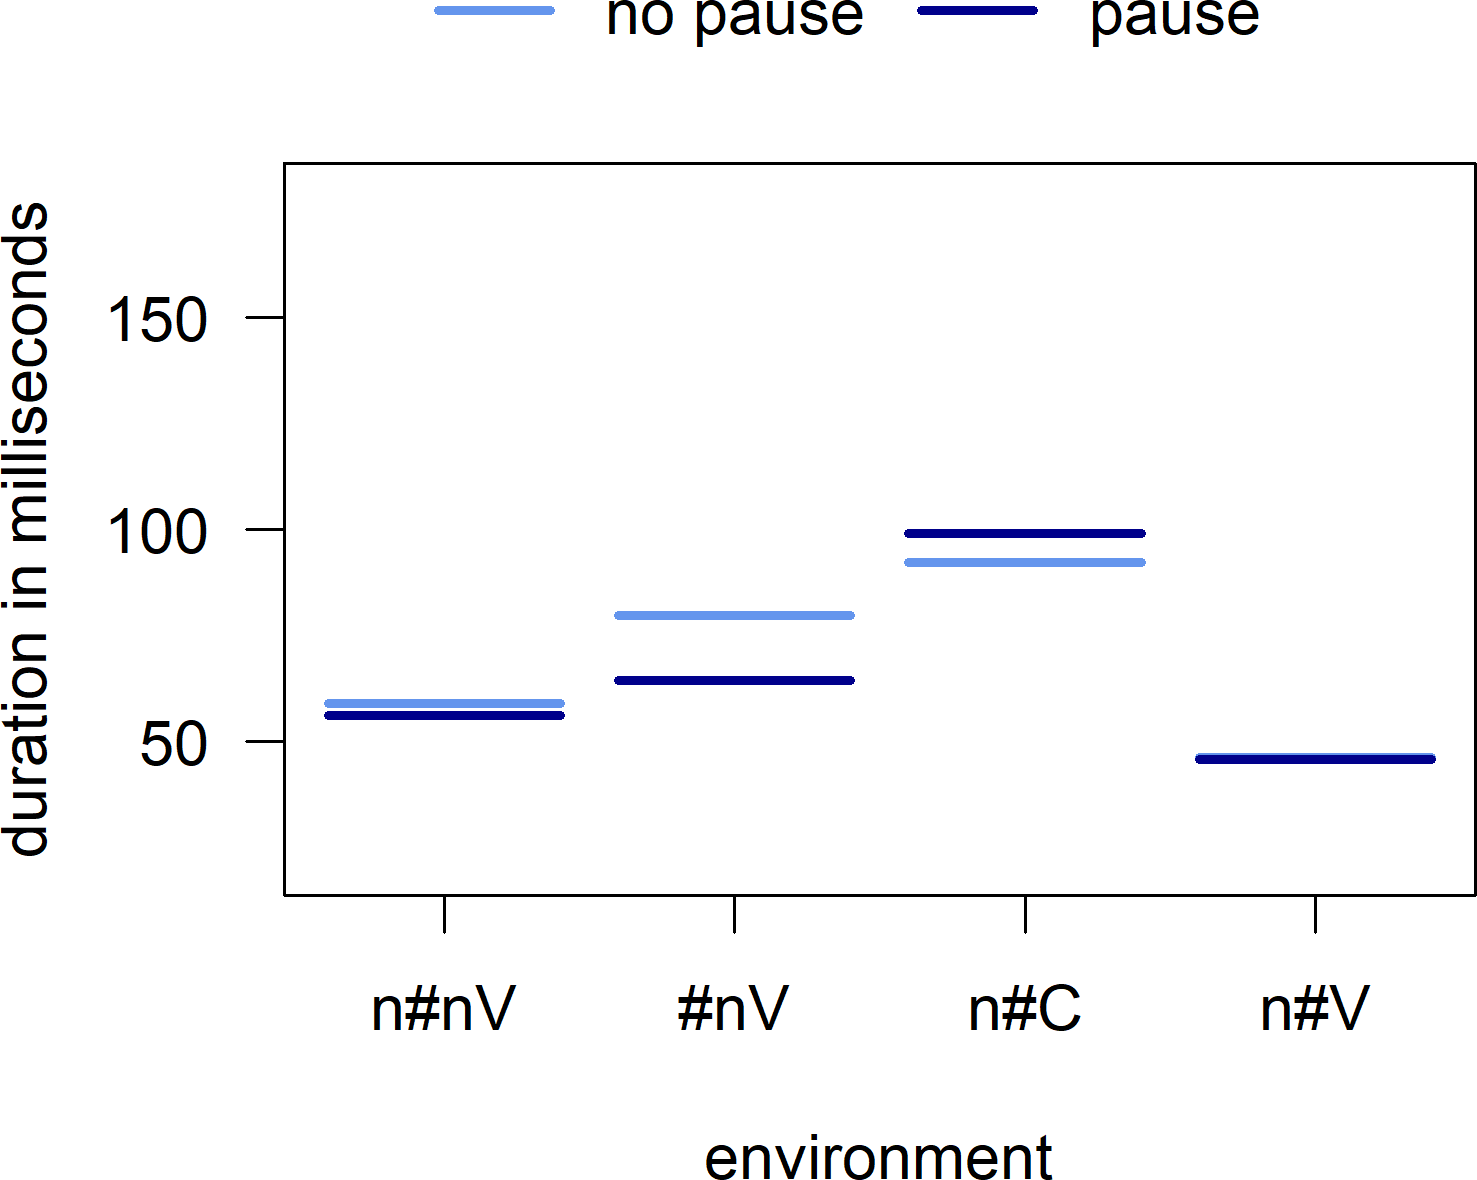
\includegraphics [scale=0.5] {images/Experiment/InModelCompleteInterEnvPause}
	\caption{Effect of pause before item by environment on consonant duration in /ɪn/-data set}
	\label{fig:Env Pause In complete experiment}
\end{figure*}	




As with the complex model, the results of the complete /ɪn/-model show that only when the base-initial syllable of a complex word is \is{stress}stressed, phonological doubles with /ɪn/ are longer than singletons in complex words followed by a vowel. 
Phonological doubles are never longer than singletons in complex words followed by a consonant or singletons in base words. 
This suggests that \isi{gemination} with \is{in-}\prefix{in} depends on the stress-pattern of the prefixed word.  Only when the base-initial syllable of a double-consonant word is \is{stress}stressed, the prefix geminates. It, furthermore, suggests that \isi{gemination} with \is{in-}\prefix{in} is weaker than \isi{gemination} with \is{un-}\prefix{un}.


In contrast to morphological geminates with \is{un-}\prefix{un}, 
morphological geminates with /ɪn/ are not longer than all types of singletons, i.e. they are not longer than singletons in base words and they are not longer than singletons in prefixed words followed by a consonant. 
That doubles with /ɪn/ are not longer than singletons followed by a consonant could be attributed to a lengthening effect caused by the following consonant.
It is expected that nasals followed by a consonant are longer than nasals followed by a vowel (see, for example, \citealt{Umeda.1977}, see also discussion in \sectref{variables of interest}).  Thus, singletons followed by a consonant might only be as long as doubles because they are lengthened by the following consonant. However, for \is{un-}\prefix{un} this lengthening effect did not result in a lack of durational difference between doubles and singletons followed by a consonant, but only in smaller durational differences between doubles and singletons.  

That \is{un-}\prefix{un} geminates to a higher degree than \is{in-}\prefix{in} is also suggested by the fact that the durational differences between doubles and singletons for /ɪn/ are much smaller than the ones for \is{un-}\prefix{un} (\isi{singleton-geminate ratio} for \is{un-}\prefix{un}: 1:3.0, \isi{singleton-geminate ratio} for /ɪn/: 1:1.6). 
The AIC increase analysis also supports the idea that \isi{gemination} is less strong with /ɪn/. It revealed that the variable \textsc{Environment} is of less importance in the /ɪn/-model than in the \is{un-}\prefix{un}model.




However, before coming to a conclusion with regard to the \isi{gemination} pattern of \is{in-}\prefix{in}, one must take a few additional facts into consideration. 
First, there are only four types of /ɪn/-prefixed words with a double consonant in the data set (\textit{innervate}, \textit{innocuous}, \textit{innominate}, \textit{innumerable}). Three of them feature a \is{stress}stressed base-initial syllable. This means that there is only one /ɪn/-prefixed type that does not geminate. It seems rather bold to make generalizations based on this one type. 
Second, as /ɪn/ is only one of several allomorphs of the prefix \is{in-}\prefix{in}, and as the \isi{gemination} of the prefix \is{in-}\prefix{in} is expected to follow similar patterns across allomorphs, 
a final conclusion with regard to the \isi{gemination} pattern of \is{in-}\prefix{in} can only be drawn after more empirical facts are revealed, i.e. after the results of the \is{im-}/ɪm/ -models are discussed.
%


\subsubsection{The allomorph /ɪm/: Complex model}


%Intro
The model predicting consonant duration with all complex \is{im-}/ɪm/ -words ($N=1177$) was fitted according to the modeling procedure described in \sectref{stats}.
Because the initial model showed a non-normal distribution,  24 outliers (2.04\% of the data) were removed and the dependent variable was Box-Cox-transformed ($\lambda = 0.101$).  
After the model was refitted with the transformed dependent variable, it showed a satisfactory distribution of residuals. The model was then simplified and interactions were tested (see \hyperref[Appendix G Summaries of tested interactions in experimental study]{Appendix G} for a list of all tested interactions). 
The \is{decomposability measure}decomposability variables were tested individually.



%Covariates
The final model features five variables, \textsc{Environment}, \textsc{BaseInitialStress}, \textsc{Accentuation}, \textsc{LocalSpeechRate} and \textsc{GlobalSpeechRate}. There are two interactions in the model, one between \textsc{BaseInitialStress} and \textsc{Accentuation}, and one between \textsc{BaseInitialStress} and \textsc{Environment}. The model is shown in \tabref{model im complex experiment} in \hyperref[Appendix H: Model Summaries Experiment]{Appendix H}.

The two noise variables \textsc{LocalSpeechRate} and \textsc{GlobalSpeechRate} show the expected effects. With increasing \isi{speech rate}, the nasal becomes shorter.
 The other two noise variables \textsc{BaseInitialStress} and \textsc{Accentuation} interact. In \is{accentuation}accented position, nasals are longer when the base-initial syllable of a word is \is{stress}stressed. In unaccented position, the opposite is the case, i.e. words with an unstressed base-initial syllable feature longer nasals than words with a \is{stress}stressed base-initial syllable. 
 


%Effect Environment
As in the /ɪn/-models, the variable of interest \textsc{Environment} interacts with \textsc{BaseInitialStress}. The effect is shown in \figref{fig:NumNasal imComplex experiment}. 
The light blue lines represent the estimated nasal durations for items with a \is{stress}stressed base-initial syllable, the dark blue lines represent  the estimated durations for items with an unstressed base-initial syllable.
The figure clearly shows that 
 only when the base-initial syllable is \is{stress}stressed, doubles are  longer than singletons. When the base-initial syllable is unstressed, doubles are shorter than singletons. 
Thus, as with /ɪn/, \isi{gemination} seems to depend on the \isi{stress} status of the base-initial syllable of a word. Only when it is \is{stress}stressed, the prefix \is{in-}\prefix{in} geminates.

 \begin{figure*}
 	
 	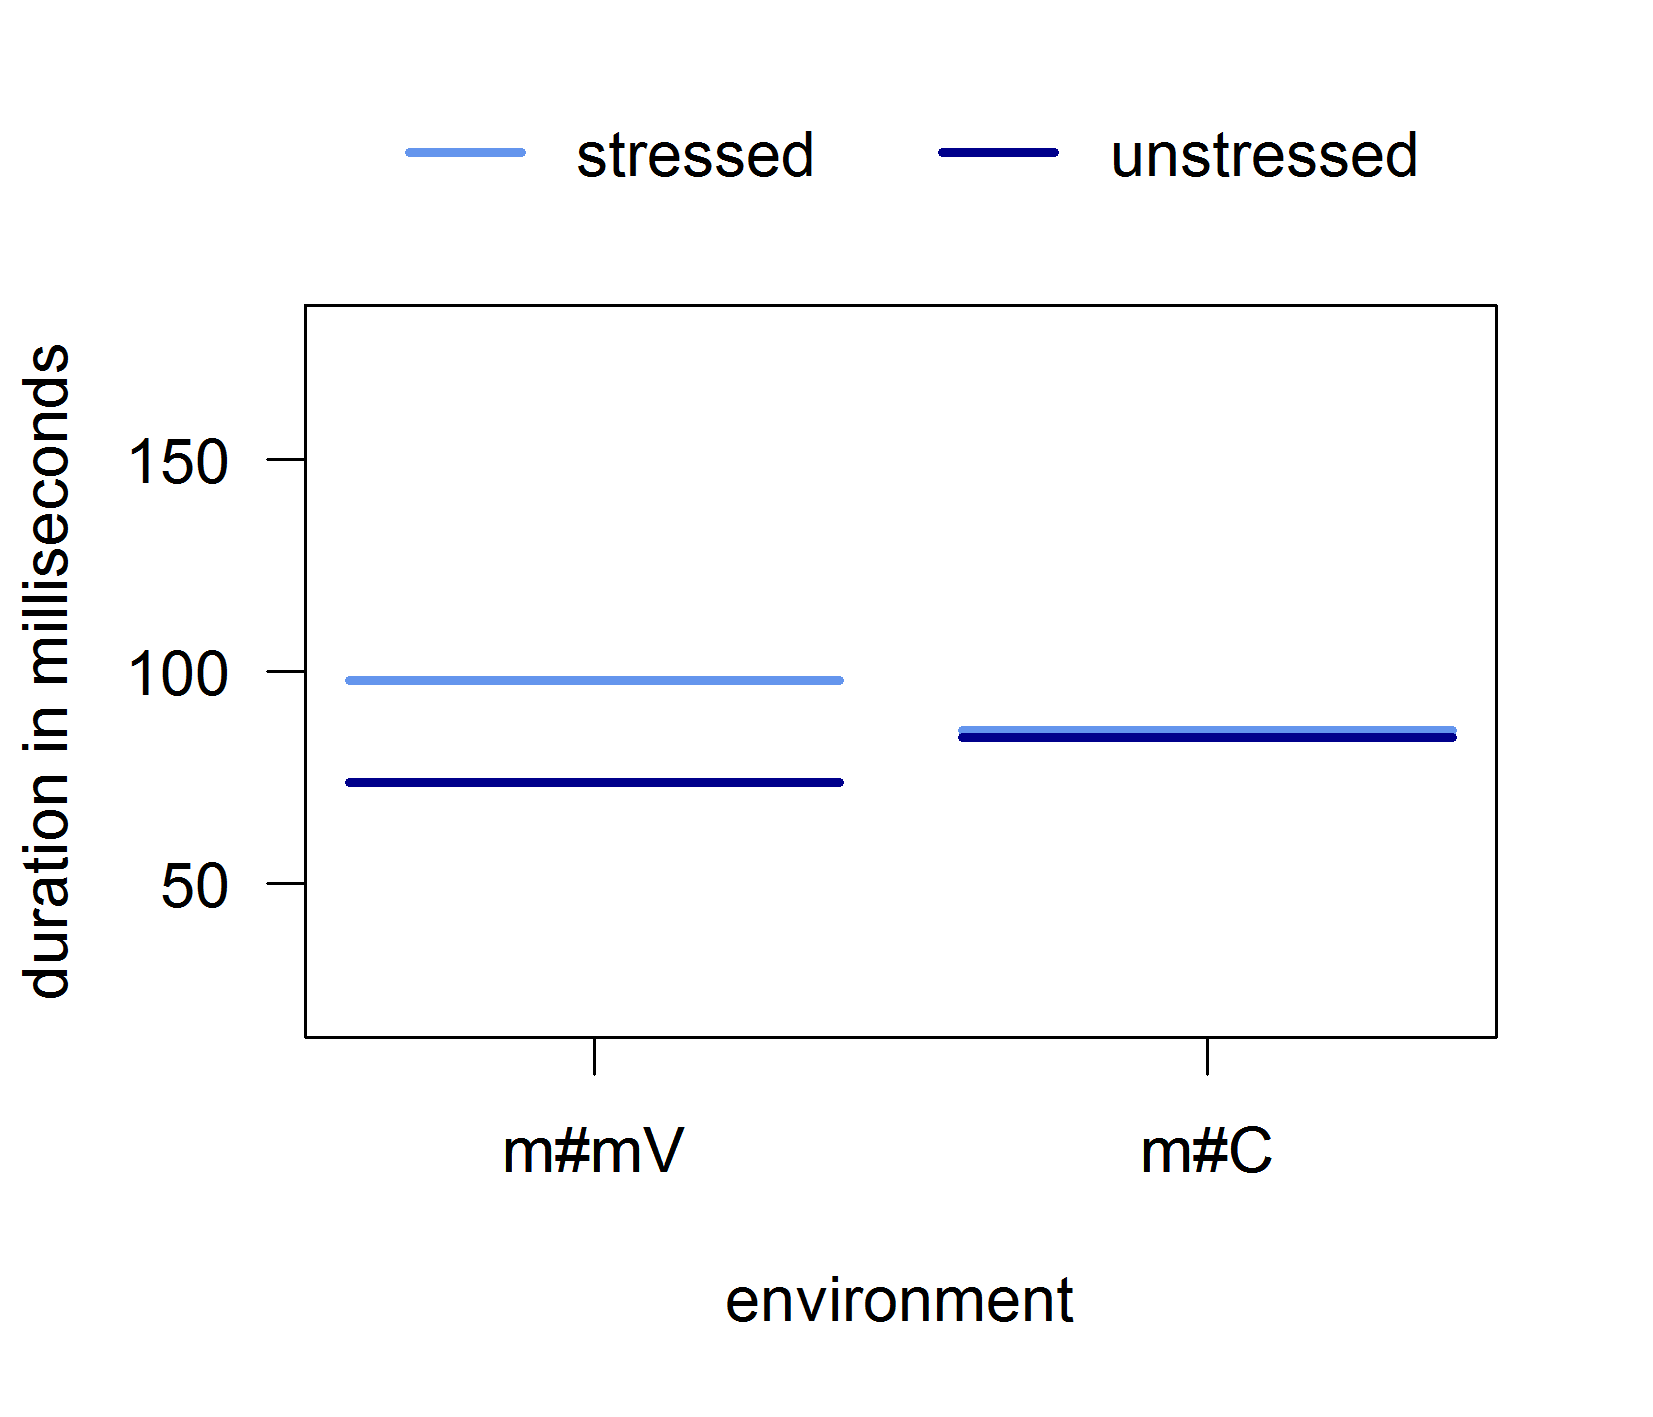
\includegraphics [scale=0.5] {images/Experiment/imModelInterEnvStress}
 	\caption{Effect of base-initial stress by environment on consonant duration in complex /ɪm/-data set}
 	\label{fig:NumNasal imComplex experiment}
 	
 \end{figure*}



The durational differences between doubles and singletons are rather small.  When the base-initial syllable is \is{stress}stressed, doubles are 12~ms longer than singletons. When the base-initial syllable is unstressed, doubles are 10~ms shorter than singletons. 
  One could explain these small differences by referring to the difference in the following segment between doubles and singletons in the \is{im-}/ɪm/ -data set. Doubles are always followed by a vowel, and singletons are always followed by a consonant. As shown in the corpus and the experimental study with \is{un-}\prefix{un} and /ɪn/, following vowels shorten the preceding nasal, i.e. the double, and following consonants lengthen the preceding nasal, i.e. the singleton. One might thus suspect that if one kept the environment constant for doubles and singletons, the durational difference between doubles and singletons in words with a \is{stress}stressed base-initial syllable would be larger, and doubles in words with an unstressed base-initial syllable would not be shorter than singletons. 

However, if one compares the results with the ones of the \is{im-}/ɪm/ -corpus study, one can see that the durational difference between doubles and singletons followed by a consonant was much larger in the corpus study (27~ms). Furthermore, in the corpus study \isi{gemination} was not dependent on the \isi{stress} status of the base-initial syllable.
It thus seems that \isi{gemination} with \is{im-}/ɪm/  differs between corpus and experimental data. In the corpus, \isi{gemination} with \is{im-}/ɪm/  is stronger and independent of prosodic factors, whereas in the experimental data \isi{gemination} is weaker and depends on base-initial \isi{stress}.


\begin{figure*}
	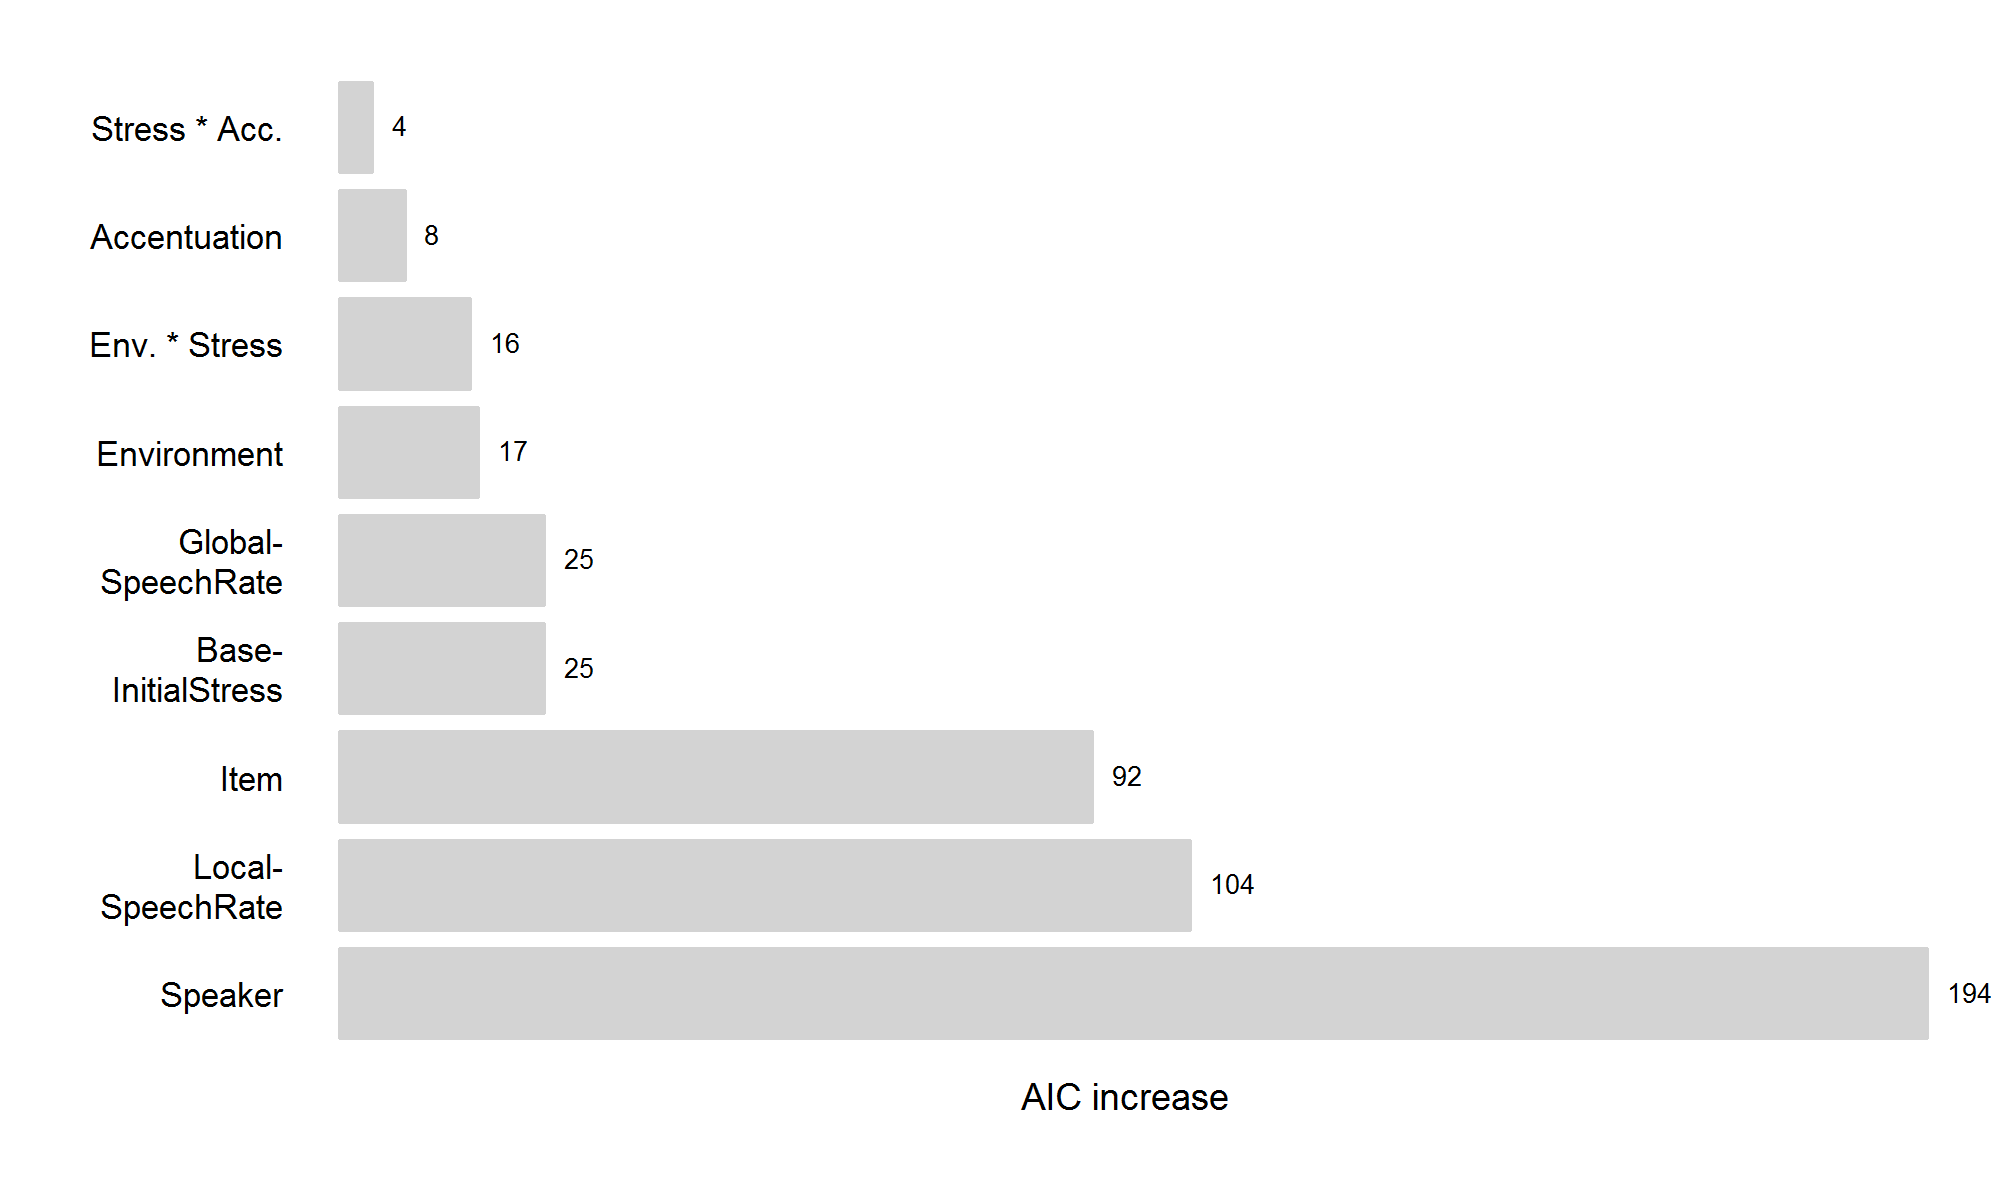
\includegraphics[scale=0.7]{images/Experiment/AICdecreaseImComplex.png}
	\caption{AIC increase for each variable of the final /ɪm/-model, AIC final model = -6389}
	\label{fig:Effectsize im experiment}
\end{figure*}

% Ind. Contribution
To test the relative importance of each term in the final model, I looked at each term's contribution to the AIC of the final model. \figref{fig:Effectsize im experiment} displays the increase of the model's AIC  without each term. 
The figure shows that the noise variables \textsc{Speaker}, \textsc{LocalSpeechRate} and \textsc{Item} explain  most of the variation found in the data. They are followed by the two noise variables \textsc{GlobalSpeechRate} and \textsc{BaseInitialStress}. The variable of interest \textsc{Environment} explains much less of the variance found in the data. The analysis of the AIC increase thus shows that most of the variation in the data is explained by noise variables, i.e. not by the variable \textsc{Environment}. This supports the idea that \isi{gemination} with \is{im-}/ɪm/  is weaker in the experimental study than in the corpus study, and that, as proposed in the previous section, \isi{gemination} with the prefix \is{in-}\prefix{in} is weaker than \isi{gemination} with the prefix  \is{un-}\prefix{un}. 




% PC
None of the \is{decomposability measure}decomposability measures showed a significant effect in the final model when tested individually. To test possible effects of a combined \isi{decomposability} measure, an additional mixed model with combined \is{decomposability measure}decomposability measures was fitted to the data set.  
To attain these combined \is{decomposability measure}decomposability measures, I fitted a principal components analysis to the scaled variables scaled\textsc{Affix}, scaled\textsc{RelativeFrequency}, scaled\textsc{SemanticTransparencyRating}, scaled\textsc{Type-OfBase} and scaled\textsc{SemanticTransparency}.





\tabref{tbl: summary PC im exp} summarizes the principal components analysis. In the upper part of the table the loadings of each \is{principal component analysis}principal component are shown. The lower part of the table displays the proportion of variance accounted for by each component. 
Most of the variance is explained by the first \is{principal component analysis}principal component. The second, third and fourth component explain much less of the variance and the fifth hardly any.  The first four components were tested in the model. 


\begin{table}
	\caption{Summary of principal components}
	\label{tbl: summary PC im exp}
	\resizebox{\textwidth}{!}{%		
		\begin{tabular}{l *{5}{S[table-format=+1.3]}}
			\lsptoprule
			 &  {PC1} &   {PC2} &  {PC3} & {PC4} & {PC5}  \\
			\midrule
			\multicolumn{6}{l}{Composition of principal components}\\\midrule
			scaled\textsc{Affix } & 0.437 & -0.407 & 0.154 & -0.785 & 0.056 \\ 
			scaled\textsc{RelativeFrequency }  & 0.314 & 0.808 & 0.407 & -0.147 & 0.247 \\ 
			scaled\textsc{SemanticTransparencyRating}  & 0.431 & 0.275 & -0.851 & -0.076 & -0.090 \\ 
			scaled\textsc{TypeOfBase }& 0.526 & -0.070 & 0.291 & 0.335 & -0.722 \\ 
			scaled\textsc{SemanticTransparency } & 0.497 & -0.317 & 0.038 & 0.494 & 0.637 \\ 			
			\midrule
			\multicolumn{6}{l}{Variance explained by principal components}\\
			 &  {PC1} &   {PC2} &  {PC3} & {PC4} & {PC5}  \\
			\midrule
			Proportion of Variance &0.542 & 0.185 & 0.117 & 0.102 & 0.054\\
			\lspbottomrule

			
		\end{tabular}
} 
	
\end{table}



This first component is composed of all five measures. This can be as seen by its loadings which are roughly the same for all variables. The second component is dominated by the variables scaled\textsc{RelativeFrequency} and scaled\textsc{Affix}, the third by scaled\textsc{SemanticTransparencyRating} and the fourth by scaled\textsc{Affix}, scaled\textsc{TypeOfBase} and scaled\textsc{SemanticTransparency}. 


The model with the principal components was fitted similarly to the model with the individual \is{decomposability measure}decomposability measures. After I simplified the model, it turned out that all terms which are significant in the final model with the individual \is{decomposability measure}decomposability measures are also significant in the final model with the principal components. On top of the effects significant in the model with the individual measures, the \is{principal component analysis}{principal component model} shows an effect of the fourth \is{principal component analysis}principal component (see \tabref{model im PC Experiment} in \hyperref[Appendix H: Model Summaries Experiment]{Appendix H} for a summary of the final model). \figref{fig:PC 4 imComplex experiment} shows the effect of \textsc{PC4}.

\begin{figure*} 
	

	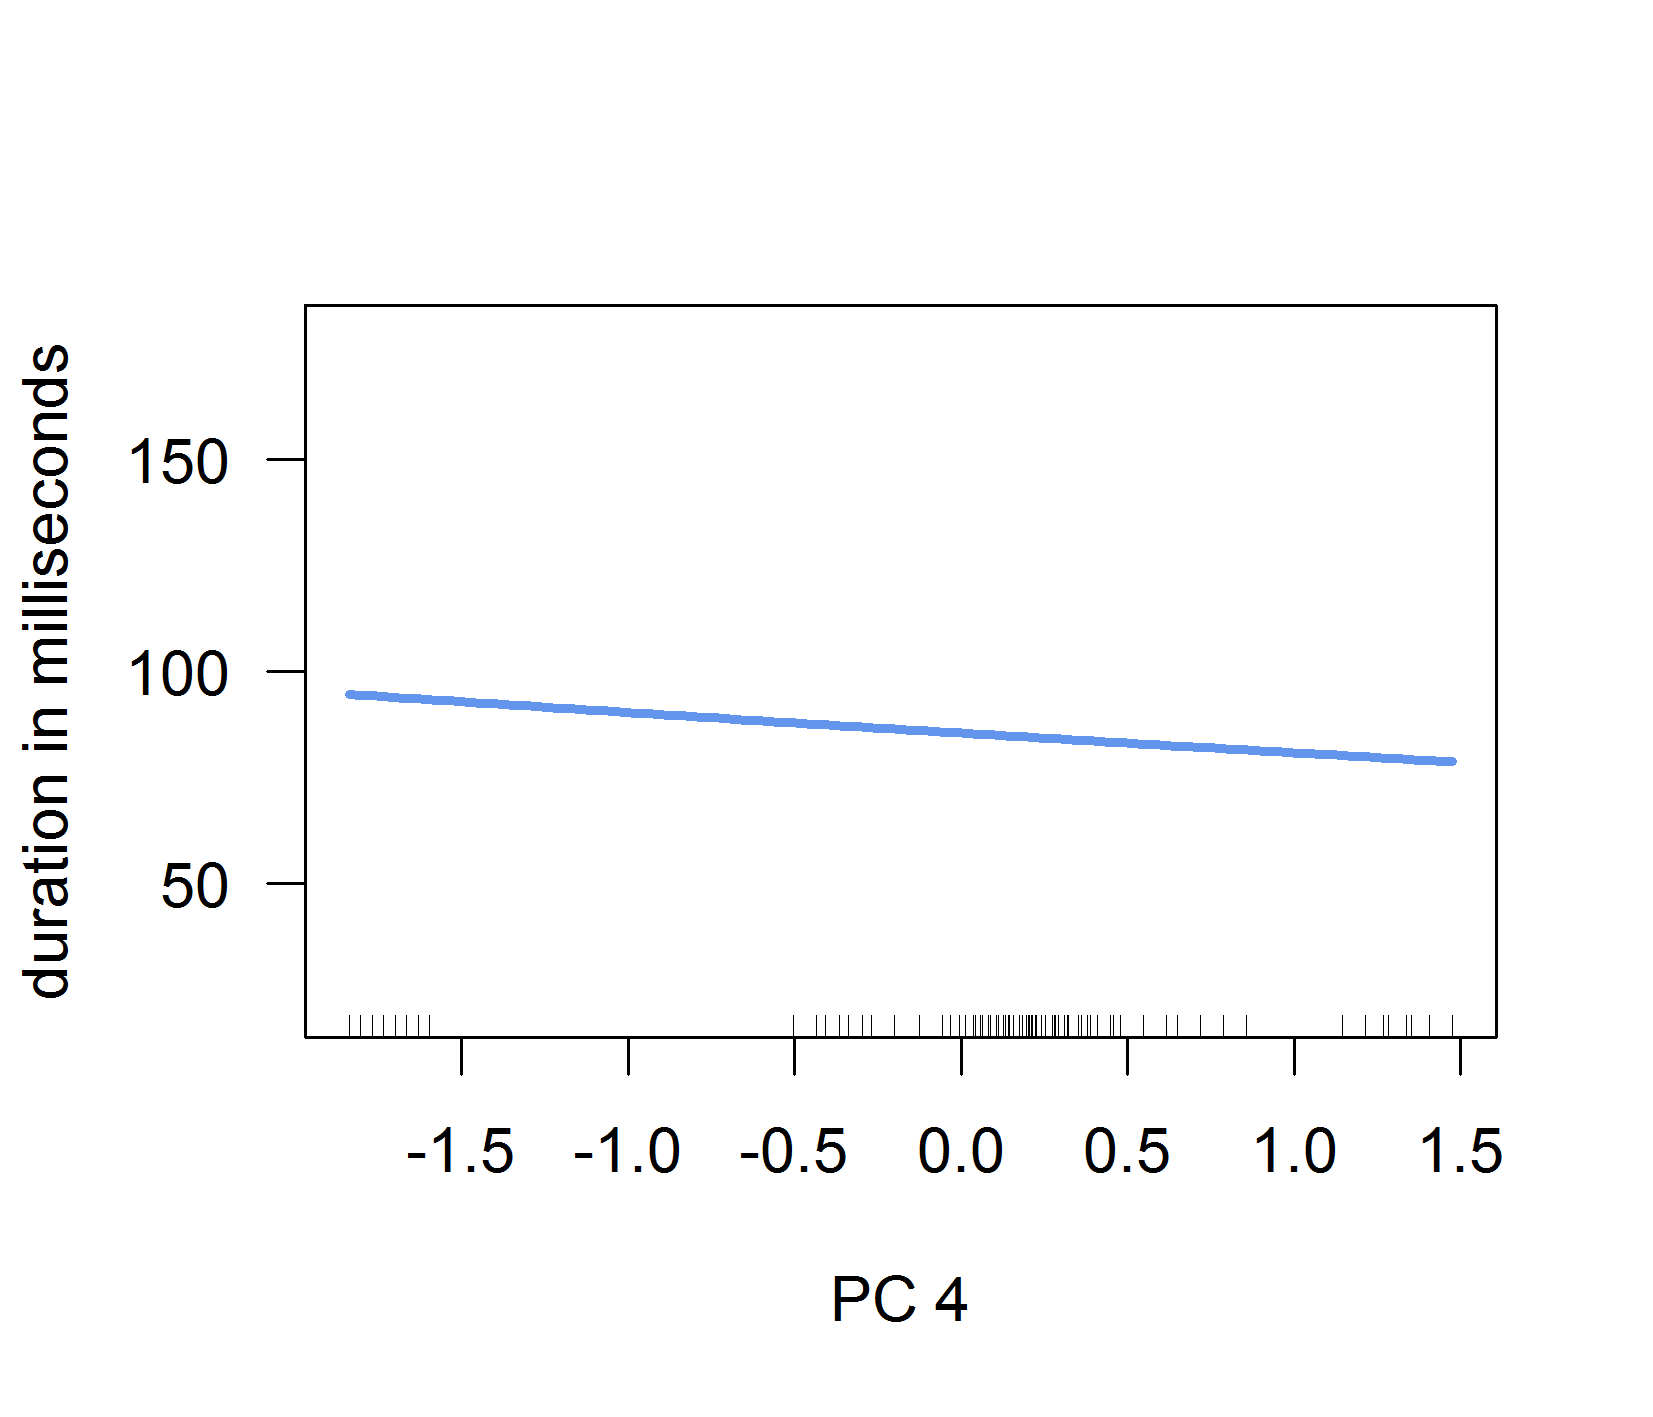
\includegraphics [scale=0.5] {images/Experiment/imModelPC}
	\caption{Effect of PC4 on consonant duration in complex /ɪm/-data set}
	\label{fig:PC 4 imComplex experiment}

\end{figure*}


The figure shows that with an increasing \textsc{PC4}-value, the nasal in /ɪn/-prefixed words becomes shorter. The size of the effect is, however, rather small. 
As described above, \textsc{PC4} is mostly composed of the variables \textsc{Affix}, \textsc{SemanticTransparency} and \textsc{TypeOfBase}. As indicated by the loadings shown in \tabref{tbl: summary PC im exp}, the component negatively correlates with \textsc{Affix}, meaning that a higher \textsc{PC4}-value represents \is{negative in-}negative \prefix{in}, and a lower value represents \is{locative in-}locative \prefix{in}. For \textsc{Semantic- Transparency} and \textsc{TypeOfBase}, the component shows positive loadings. This means that a higher \textsc{PC4}-value represents opaque derivatives with a bound base, and that a lower \textsc{PC4}-value represents transparent derivatives with words as bases.
The effect of \textsc{PC4} on nasal duration can thus be interpreted as follows: nasals in opaque \is{negative in-}negative \prefix{in}prefixed words with a bound base tend to be shorter than nasals in transparent \is{locative in-}locative \prefix{in}prefixed words with words as bases. This interpretation is supported by the fact that all tokens with a \textsc{PC4}-value lower than $-1.5$ are \is{locative in-}locative \prefix{in}prefixed words with a word as a base and transparent meaning (e.g. \textit{implant, imprison}). It is yet unclear why these words feature a particularly long nasal. 
It seems though that \textsc{PC4} reflects an effect on prefixal consonant duration that is restricted to a small number of types with a particular feature combination. This feature combination does not appear to directly translate to \isi{decomposability}.  
Instead, it might be related to the existence of two different \is{locative in-}locative \prefix{in}prefixes. 

As discussed in \sectref{locative in}, there might be two distinct \is{locative in-}locative \prefix{in}prefixes: native and non-native \is{locative in-}locative \prefix{in}. The two types of \is{locative in-}locative \prefix{in} are argued to differ in their origin, the type of base they take and their \isi{productivity}. The items with a low \textsc{PC4}-value seem to represent items with native \is{locative in-}locative \prefix{in}, i.e. \is{locative in-}locative \prefix{in}items with a transparent meaning and a native and free base. (e.g. \textit{implant}, \textit{imprison}). It remains unclear why they feature particularly long nasals.



To summarize,  doubles with the allomorph \is{im-}/ɪm/  are only longer than singletons in complex words when the base-initial syllable of the derivative is \is{stress}stressed. This is similar to what was found with the allomorph /ɪn/. The singleton-gemi-nate ratio for \is{im-}/ɪm/  in the experimental study is smaller than the one found in the corpus study, and also smaller than the one found for \is{un-}\prefix{un}. 
The model which tested combined \is{decomposability measure}decomposability measures furthermore shows a significant effect of one \is{principal component analysis}principal component on nasal duration with \is{im-}/ɪm/. However, the effect is relatively small and not clearly interpretable in terms of \isi{decomposability}. Crucially, the effect does not affect \isi{gemination}.




\subsubsection{The allomorph /ɪm/: Complete model}

The model predicting consonant duration with all \is{im-}/ɪm/-words ($N=1635$) was fitted according to the modeling procedure described in \sectref{stats}.  Because the initial model showed a non-normal distribution,  37 outliers (2.63\% of the data) were removed and the dependent variable was Box-Cox transformed ($\lambda = 0.343$). 
After the transformation, the model showed a satisfactory distribution of residuals. The model was then simplified and interactions were tested (see \hyperref[Appendix G Summaries of tested interactions in experimental study]{Appendix G} for a list of all tested interactions). 

 
The final model features the five variables \textsc{Environment}, \textsc{BaseInitialStress}, \textsc{PrePause}, \textsc{LocalSpeechRate} and \textsc{GlobalSpeechRate} (see \tabref{model im complete experiment} in \hyperref[Appendix H: Model Summaries Experiment]{Appendix H} for a summary of the final model). Both \is{speech rate}speech rates show the expected effects. With increasing \is{speech rate}speech rates, the nasal becomes shorter. The three variables \textsc{Environment}, \textsc{BaseInitialStress}, and \textsc{Pause} form a three-way interaction. The interaction is shown in \figref{fig:NumNasal imCompleteexperiment}.

\begin{figure*}
	
	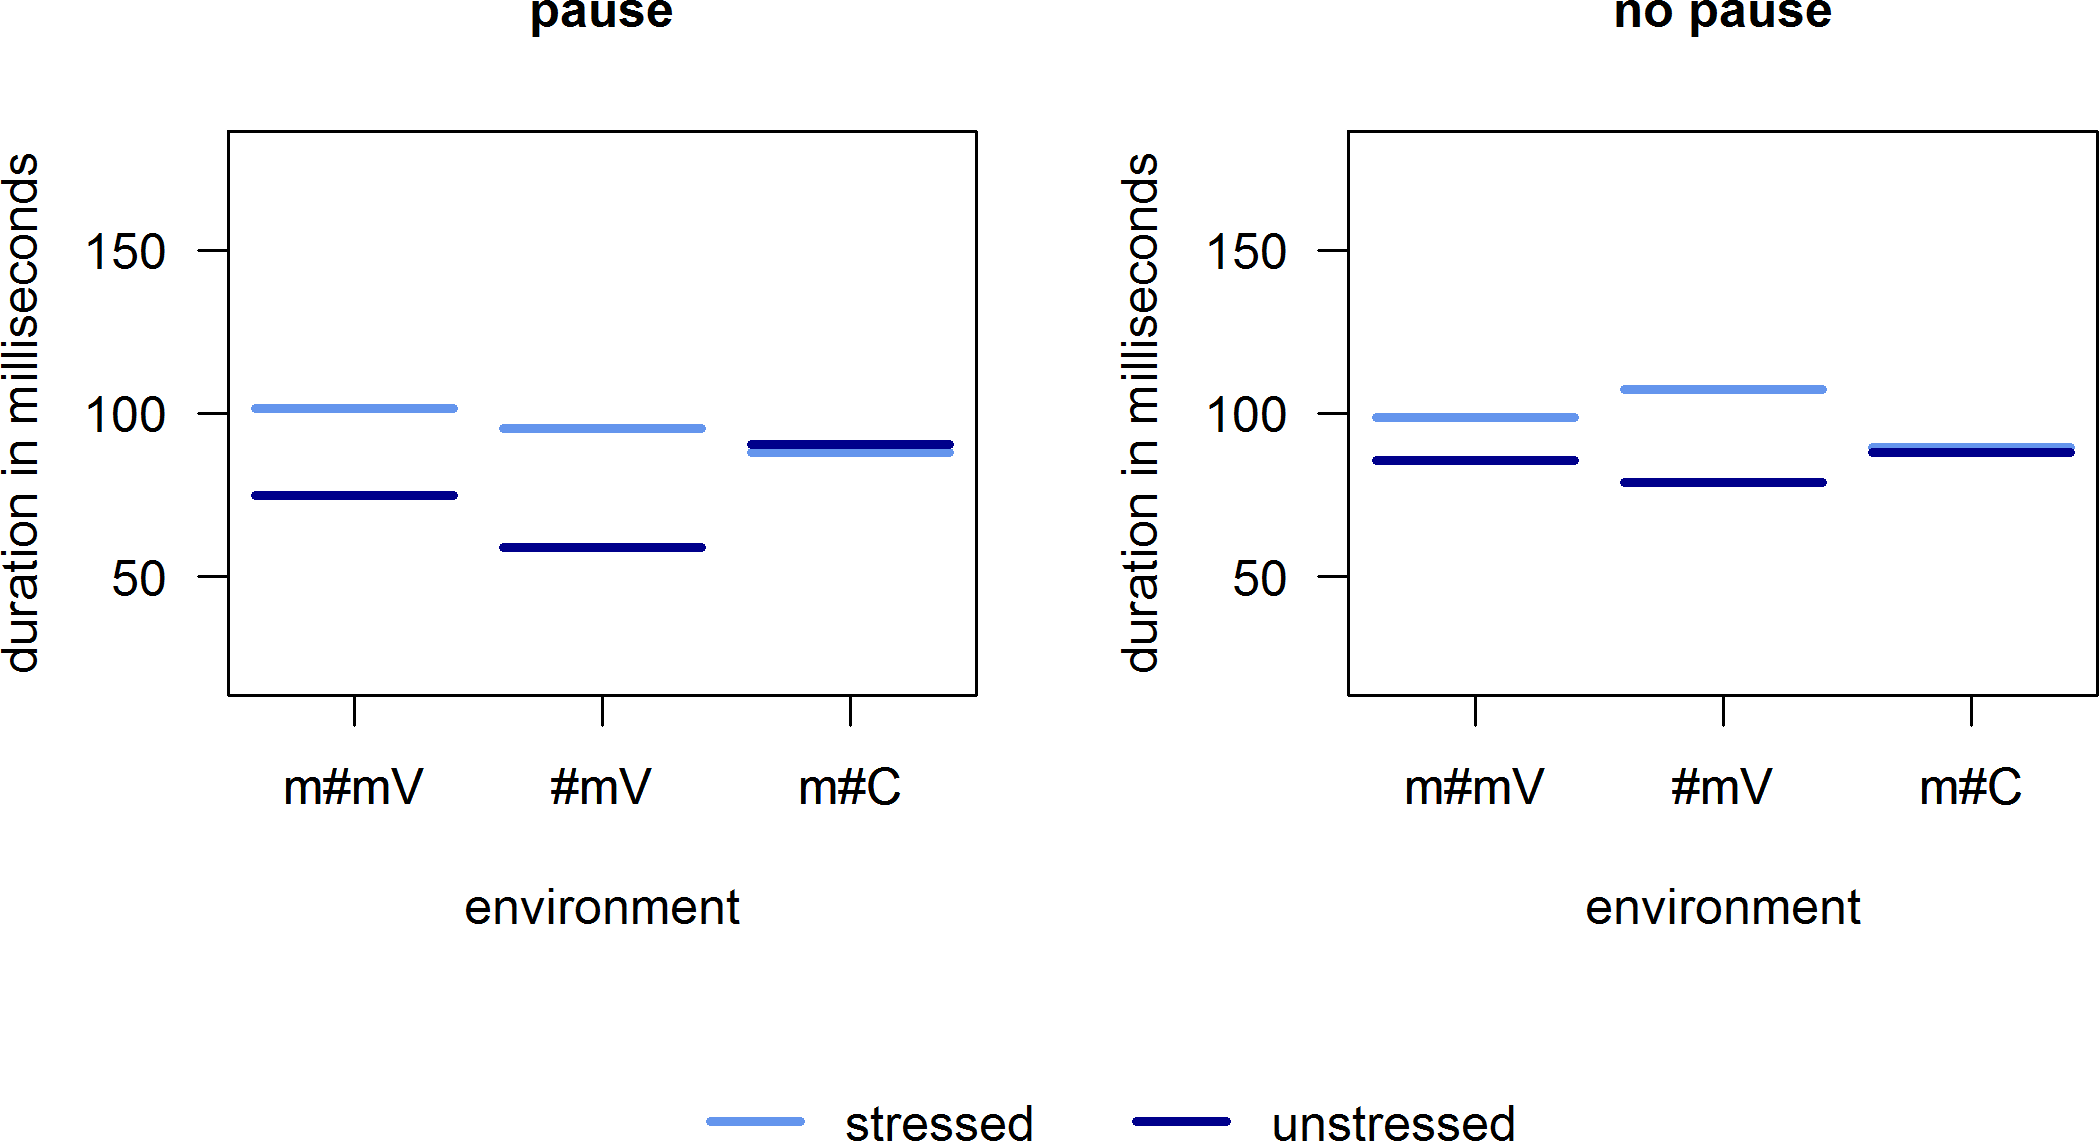
\includegraphics [scale=0.6] {images/Experiment/imModelCompleteInterEnvStressPause}
	
	\caption{Effect of base-initial stress by environment on consonant duration in /ɪm/-data set}
	\label{fig:NumNasal imCompleteexperiment}
\end{figure*}


The left panel of the figure shows the effect of \textsc{BaseInitialStress} by \textsc{Environment} for items produced with a pause before the item. The right panel shows the effect for items produced without a preceding pause. For each environment, light blue lines indicate the durations for items with a \is{stress}stressed base-initial syllable, and dark blue lines indicate the durations for items with an unstressed base-initial syllable.


In the left panel, i.e. in items with a preceding pause, doubles (\texttt{m\#mV}) are longer than singletons in base words (\texttt{\#mV}). This is independent of the \isi{stress} status of the base-initial syllable. Doubles are, however, only longer than singletons in complex words (\texttt{m\#C}) when the base-initial syllable is \is{stress}stressed.
In the right panel, i.e. in items without a preceding pause, doubles (\texttt{m\#mV}) are only longer than singletons in base words (\texttt{\#mV}) when the base-initial syllable is unstressed. In this case, they are as long as singletons in complex words (\texttt{m\#C}). For items with a \is{stress}stressed base-initial syllable, doubles (\texttt{m\#mV}) are shorter than singletons in base words (\texttt{\#mV}) but longer than singletons in complex words (\texttt{m\#C}).

To summarize, independent from a preceding pause, doubles in words with a \is{stress}stressed base-initial syllable are predicted to be longer than singletons in complex words. Depending on the absence or presence of a preceding pause, doubles in words with an unstressed base-initial syllable are either as long as or shorter than singletons in complex words. They are never predicted to be longer than singletons in complex words. 
Except for when the double consonant is part of a word which is not preceded by a pause and which features a \is{stress}stressed base-initial syllable, doubles are longer than singletons in base words with the same condition.


\subsubsection{Summary}


In all \is{in-}\prefix{in}models, the noise variables behaved as expected. Decomposability does not seem to influence nasal duration with \is{in-}\prefix{in}. Only in one model, one \isi{decomposability} measure affected nasal duration (\textsc{PC4}). Its effect was very weak and not clearly interpretable in terms of \isi{decomposability}. It did not affect \isi{gemination}.


For both allomorphs of \is{in-}\prefix{in}, the analyses have shown that doubles are only longer than singletons when the base-initial syllable of the derivative is \is{stress}stressed. These doubles are, however, only longer than some types of singletons, and durational differences between doubles and singletons are often rather small. 
In case of /ɪn/, doubles in words with a \is{stress}stressed base-initial syllable are only longer than singletons in complex words with a following vowel. Doubles are not predicted to be longer than singletons in complex words with a following consonant or singletons in base words. 
For \is{im-}/ɪm/, doubles in words with a \is{stress}stressed base-initial syllable are longer than singletons with a following consonant but the durational difference between doubles and singletons is rather small.
Furthermore, doubles are slightly longer than singletons in base words.


The results suggest that \isi{gemination} with \is{in-}\prefix{in} depends on \isi{stress} and that the \isi{degree of gemination} with \is{in-}\prefix{in} is rather weak. Only when the base-initial syllable of a word is \is{stress}stressed, doubles are longer than some types of singletons, i.e. for /ɪn/, they are longer than singletons in complex words followed by a vowel, and for \is{im-}/ɪm/, they are longer than singletons in complex words followed by a consonant. Durational differences between doubles and singletons are rather small. This result is quite different from what was found for \is{un-}\prefix{un}. For \is{un-}\prefix{un}, doubles are longer than all types of singletons and the durational differences between doubles and singletons are much larger. One can thus state that the prefix \is{in-}\prefix{in} geminates, but that it geminates to a lesser degree than the prefix \is{un-}\prefix{un}.

Interestingly, the \isi{gemination} pattern found for \is{in-}\prefix{in} in the experimental study deviates from the one found in the corpus study. In the corpus study, \is{in-}\prefix{in} geminates independent of \isi{stress}, durational differences between doubles and singletons are bigger, and the \isi{degree of gemination} is the same as for \is{un-}\prefix{un}. In other words, \isi{gemination} with \is{in-}\prefix{in} is weaker in the experimental study than in the corpus study.

One possible explanation for the difference between corpus and experimental data is that the degree of \isi{semantic processing} differs between the two types of investigated speech. It can be hypothesized that in natural, \isi{conversational speech},  the \isi{semantic processing} of words is deeper than in \isi{read speech}, and that processing depth, in turn, affects \isi{gemination}. With deeper processing, the meaning of the affix is more present in the production of the derivative, leading to less \isi{reduction}, i.e. to \isi{gemination}. 
 In the corpus study, the meaning of the prefix is deeply processed, and it therefore clearly geminates. In the experimental study, in contrast, the affix's meaning is not processed deeply. In turn, \isi{gemination} is weaker and governed by a non-semantic factor,  i.e. the prosodic factor \isi{stress}.
  This explanation is supported by the fact that the variable \textsc{Affix} (\is{locative in-}locative \prefix{in} vs. \is{negative in-}negative \prefix{in}) only affects consonant duration with \is{in-}\prefix{in} in the corpus study, not in the experimental study. The meaning of the affix only affects consonant duration in the corpus data, where it is semantically processed. It does not affect consonant duration in the experimental data, where no deep \isi{semantic processing} takes place.





\subsection{The prefixes \prefix{un} and \prefix{in}}
The model predicting consonant duration with all complex \is{un-}\prefix{un} and /ɪn/-words ($N=3237$) was fitted to directly compare \isi{gemination} with \is{un-}\prefix{un} and \is{in-}\prefix{in}, and to further investigate the observed differences between the affixes.
As already discussed in \sectref{corpus un in}, in a model which investigates both prefixes, the \is{decomposability measure}decomposability variables cannot be tested in an interesting way. This is because \is{un-}\prefix{un}, as described in Sections~\ref{The decomposability of the four affixes: a comparison} and~\ref{decomposability experiment}, does not vary in most of the \is{decomposability measure}decomposability measures, and because \isi{relative frequency} measures are not well comparable across \is{un-}\prefix{un} and \is{in-}\prefix{in}. The prefix \is{in-}\prefix{in} has very many bound roots, which is problematic with regard to computing \isi{relative frequency} measures that are comparable to the \isi{relative frequency} measures of affixes with hardly any or no bound roots, i.e. in this case \is{un-}\prefix{un}. Therefore, none of the \is{decomposability measure}decomposability measures was tested in the model. 

 The model was fitted according to the modeling procedure described in \sectref{stats}. Due to an uneven distribution of the residuals in the initial model, the dependent variable \textsc{AbsoluteConsonantDuration} was Box-Cox-transformed ($\lambda = 0.061$) and 67 outliers were removed (2.07\% of the data).
The model was then simplified and interactions were tested (see \hyperref[Appendix G Summaries of tested interactions in experimental study]{Appendix G} for a list of all tested interactions).


The final model features the five variables \textsc{Environment}, \textsc{Affix}, \textsc{PrePause}, \textsc{Accentuation} and \textsc{LocalSpeechRate}. The variable \textsc{LocalSpeechRate} has the expected effect. The three variables \textsc{Environment}, \textsc{Affix} and \textsc{PrePause} interact. Furthermore, there is an interaction between \textsc{Environment} and \textsc{Accentuation}. The final model is summarized in \tabref{model in un experiment} in \hyperref[Appendix H: Model Summaries Experiment]{Appendix H}.


\figref{fig: Un In experiment Env and accent} shows the interaction between \textsc{Environment} and \textsc{Accentuation}. Estimates for \is{accentuation}accented items are shown in light blue, and estimates  for unaccented items are shown in dark blue. The figure shows that, independent of \isi{accentuation}, doubles (\texttt{n\#nV}) are clearly longer than singletons (\texttt{n\#C}, \texttt{n\#V}). In \is{accentuation}accented position, doubles are even longer. This has the effect that the durational difference between doubles and singletons increases in \is{accentuation}accented condition.



\begin{figure*}
	
	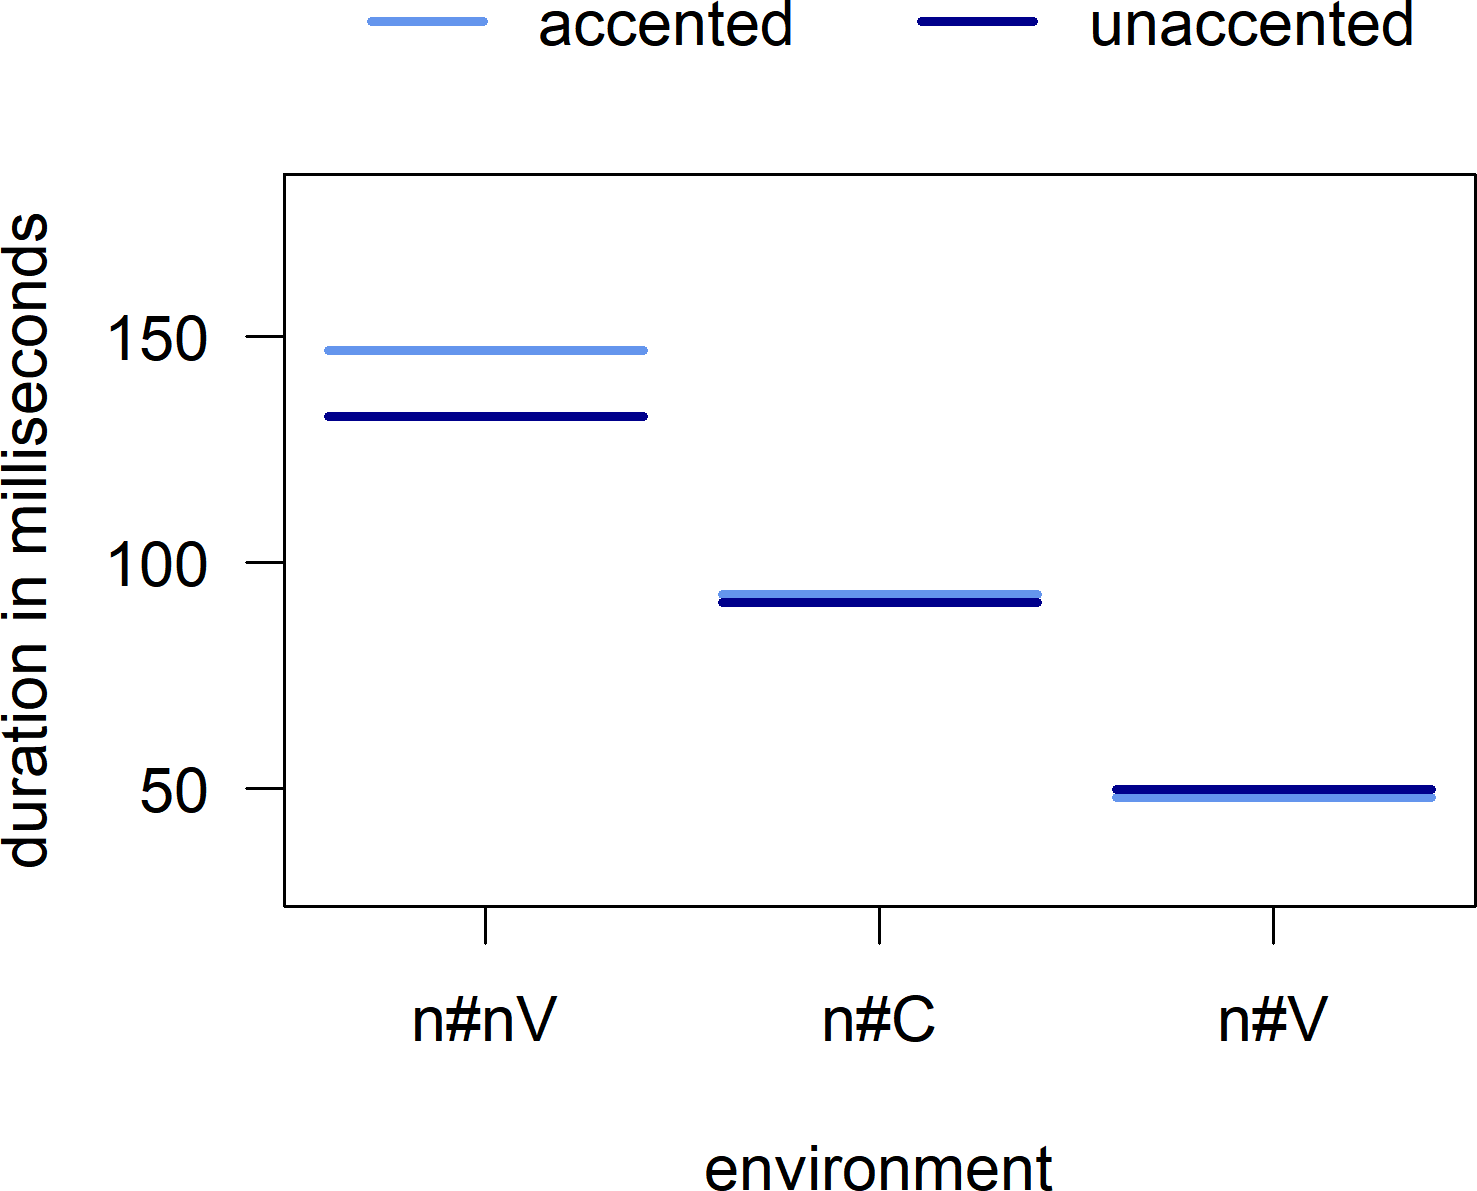
\includegraphics [scale=0.5] {images/Experiment/UnInInterEnvAcc}
	\caption{Effect of accentuation by environment on consonant duration in complex \prefix{un} and /ɪn/-words}
	\label{fig: Un In experiment Env and accent}
\end{figure*}

 However, to really interpret the \isi{gemination} pattern of the affixes, one must consider the three-way interaction between \textsc{Environment}, \textsc{Affix} and \textsc{PrePause}. The interaction is displayed in \figref{fig:Un In experiment}. In the left panel of the figure, the estimates for items with a preceding pause are shown. In the right panel of the figure, the estimates for items without a preceding pause are shown. For each affix, estimates for double consonants are shown in light blue, estimates for singletons followed by a consonant are shown in green, and estimates for singletons followed by a vowel are shown in dark blue.






\begin{figure*}
	
	\includegraphics [scale=0.6] {images/Experiment/UnInInterEnvAffixPause1}
	
	\caption{Effect of environment by affix on consonant duration in complex \prefix{un} and /ɪn/-words with and without a preceding pause}
	\label{fig:Un In experiment}
\end{figure*}


In both panels of the figure, it is clearly visible that while the durations of the singletons do not differ much across affixes, the durations of the double consonants differ a lot across affixes. The double consonant in \is{un-}\prefix{un}prefixed words is much longer than the double consonant in both \is{in-}\prefix{in}prefixed words.
The double consonant in \is{negative in-}negative \prefix{in}prefixed words is longer than the one in \is{locative in-}locative \prefix{in}prefixed words. 
As a consequence, there are differences in \isi{gemination} between the affixes. 
 The prefix \is{un-}\prefix{un} clearly geminates, i.e. doubles are clearly longer than both singleton levels. 
For \is{negative in-}negative \prefix{in}, \isi{gemination} is weaker. Doubles are longer than singletons with a following vowel (\texttt{n\#V}), and about as long as singletons with a following consonant (\texttt{n\#C}). 
The double consonant in \is{locative in-}locative \prefix{in}words is the shortest. It is only longer than singletons which are followed by a vowel (\texttt{n\#V}) and preceded by a pause. It is debatable whether this difference between doubles and singletons with \is{locative in-}locative \prefix{in} can be interpreted as \isi{gemination} at all.

At first glance, the results suggest that the \isi{degree of gemination} decreases from \is{un-}\prefix{un} to \is{negative in-}negative \prefix{in}, to \is{locative in-}locative \prefix{in}.  However, one must be cautions with this interpretation. As already mentioned before, there are only four /ɪn/-prefixed types with a double consonant in the data set. Only one of these types features \is{locative in-}locative \prefix{in}, i.e. the conclusion that \is{locative in-}locative \prefix{in} geminates to a lesser degree than \is{negative in-}negative \prefix{in} is based on only one type. Furthermore, the type featuring \is{locative in-}locative \prefix{in} is the only type with an unstressed base-initial syllable in the data set. 
It might thus be the case that the difference between locative and \is{negative in-}negative \prefix{in} is actually caused by a difference in the prosodic structure of the words, i.e. by a difference in the \isi{stress} status of the base-initial syllable. There are two arguments for this explanation. First, the analysis of all \is{in-}\prefix{in}data has already shown that \isi{gemination} with \is{in-}\prefix{in} depends on the \isi{stress} status of the base-initial syllable. The effect of \isi{stress} was observed for both allomorphs of  \is{in-}\prefix{in}. Only when the base-initial syllable is \is{stress}stressed, \is{in-}\prefix{in} geminates. 
 Second, in none of the \is{in-}\prefix{in}analyses an effect of \textsc{Affix} was found. 


One can conclude that there is a difference in the \isi{degree of gemination} between \is{un-}\prefix{un} and the \is{in-}\prefix{in}prefixes: \isi{gemination} with \is{un-}\prefix{un} is stronger than \isi{gemination} with \is{in-}\prefix{in}. This might be explained with the fact that \is{un-}\prefix{un} is more segmentable and more informative than both \is{in-}\prefix{in}prefixes. However, there is no clear evidence for different degrees of \isi{gemination} between  \is{locative in-}locative \prefix{in} and \is{negative in-}negative \prefix{in}, even though the two \is{in-}\prefix{in}prefixes differ in \isi{segmentability} and \isi{informativeness}. Gemination with \is{in-}\prefix{in} depends on prosodic structure.

 This result is different from what was found in the corpus study. In the corpus study, \isi{gemination} was the same across \is{un-}\prefix{un} and \is{in-}\prefix{in} but there was a general durational difference between the affixes. The prefix \is{un-}\prefix{un} featured the longest nasal, followed by \is{negative in-}negative \prefix{in}. Locative \prefix{in} featured the shortest nasal. 
Even though the results differ, they can be interpreted similarly: the more segmentable the affix, or the more informative, the less \isi{reduction}. In the corpus study,  \isi{reduction} affected singletons and doubles. In the experimental study, only doubles were affected and there was no distinction between negative and \is{locative in-}locative \prefix{in}.






\subsection{The prefix \textit{dis-} }


\subsubsection{Complex model}

The model predicting consonant duration with all complex \is{dis-}\prefix{dis}words ($N=829$) was fitted according to the modeling procedure described in \sectref{stats}. Due to an uneven distribution of the residuals in the initial model, the dependent variable \textsc{AbsoluteConsonantDuration} was Box-Cox-transformed ($\lambda = 0.263$) and 16 outliers were removed (1.9\% of the data). After the model was refitted with the transformed dependent variable, it showed a satisfactory distribution of residuals. The model was then simplified and interactions were tested (see \hyperref[Appendix G Summaries of tested interactions in experimental study]{Appendix G} for a list of all tested interactions). The \is{decomposability measure}decomposability variables were tested individually.

The final model features three variables, \textsc{Environment}, \textsc{LocalSpeechRate} and \textsc{Accentuation}. The variable \textsc{LocalSpeechRate} behaves as expected: the higher the \isi{speech rate}, the shorter the consonant. The variables \textsc{Environment} and \textsc{Accentuation} form an interaction. The final model is summarized in \tabref{model dis complex experiment} in \hyperref[Appendix H: Model Summaries Experiment]{Appendix H}.






\begin{figure*}
	
	\includegraphics [scale=0.5] {images/Experiment/DisModelInterEnvAcc}
	\caption{Effect of accentuation by environment on consonant duration in complex \prefix{dis}data set}
	\label{fig:NumNasal disComplex experiment}
\end{figure*}



The interaction between \textsc{Environment} and \textsc{Accentuation} is depicted in \figref{fig:NumNasal disComplex experiment}. For each environment, the estimates for \is{accentuation}accented items are shown by light blue lines, and the estimates for unaccented items are shown by dark blue lines.
The figure shows that,  
independent from \isi{accentuation}, doubles (\texttt{s\#sV-str.}) are longer than both types of singletons in complex words (\texttt{s\#V-str.}, \texttt{s\#V-unstr.}). The durational differences between doubles and singletons are larger in the \is{accentuation}accented than in the unaccented condition. 
In \is{accentuation}accented condition, doubles are 25~ms longer than singletons with a \is{stress}stressed base-initial syllable and 30~ms longer than singletons with an unstressed base-initial syllable. 
In unaccented condition, doubles are 20~ms longer than both types of singletons. 
The durational difference between the two singleton levels is not significant.

As doubles are longer than both types of singletons, one can state that \is{dis-}\prefix{dis} geminates. The durational differences between doubles and singletons are smaller than the ones found for \is{un-}\prefix{un}. They are in approximately the same range as the ones for /ɪn/. This suggests that \is{dis-}\prefix{dis} geminates to a similar degree as \is{in-}\prefix{in}.



\figref{fig:Effectsize dis experiment} shows the contribution of each variable to the final model's goodness of fit.
The figure clearly shows that the variable \textsc{Speaker} explains most of the variance found in the data. The variable 
\textsc{Environment}, i.e. the crucial variable with regard to \isi{gemination}, explains much less of the variance. This fits in well with the interpretation that the prefix \is{dis-}\prefix{dis} geminates, but that it does not geminate to a high degree.


\begin{figure*}
	
	\includegraphics[scale=0.7]{images/Experiment/AICdecreaseDisComplex.png}
	\caption{AIC increase for each variable of the final \prefix{dis}model, AIC final model = -4031}
	\label{fig:Effectsize dis experiment}

\end{figure*}



None of the individual \is{decomposability measure}decomposability variables proved to be significant in the final complex \is{dis-}\prefix{dis}model. To check whether a combined \isi{decomposability} measure affects consonant duration with \is{dis-}\prefix{dis}, I conducted a \is{principal component analysis}principal component analysis and tested the effect of the principal components in an additional model. The \is{principal component analysis}principal component analysis included the four variables log\textsc{RelativeFre-quency}, \textsc{SemanticTransparencyRating}, \textsc{TypeOfBase} and \textsc{SemanticTranspa-rency}. Categorical variables were recoded as numerical, and all variables were scaled. \tabref{tbl: summary PC dis exp} summarizes the principal components.



\begin{table*}
	\caption{Summary of principal components\label{tbl: summary PC dis exp}}
	\resizebox{\textwidth}{!}{%		
		\begin{tabular}{l *{4}{S[table-format=+1.3]}}
			\lsptoprule
			 &  {PC1} &   {PC2} &  {PC3} & {PC4}   \\
			\midrule
			\multicolumn{5}{l}{Composition of principal components}\\
			\midrule
			scaled\textsc{RelativeFrequency }  & -0.465& 0.817&0.344&0.005\\ 
			scaled\textsc{SemanticTransparencyRating}  &-0.489 &-0.559&  0.670 & 0.002 \\ 
			scaled\textsc{TypeOfBase }&-0.523& -0.098& -0.462& -0.710 \\ 
			scaled\textsc{SemanticTransparency } &-0.522& -0.104&-0.469&0.705 \\ 		
			\midrule
			\multicolumn{5}{l}{Variance explained by principal components}\\
			\midrule
			Proportion of Variance &0.644 &0.148 &0.112& 0.097\\
			\lspbottomrule			
		\end{tabular}}	
\end{table*}


Most of the variance is accounted for by the first component, the second and the third component explain much less variance, and the last \is{principal component analysis}principal component explains barely any variance. 
The first \is{principal component analysis}principal component is composed of all \is{decomposability measure}decomposability measures. The second component is mainly dominated by log\textsc{RelativeFrequency}, the third component mostly represents \textsc{TypeOfBase}, \textsc{SemanticTransparencyRating} and \textsc{SemanticTransparency}, and the fourth is mostly composed of \textsc{TypeOfBase} and \textsc{SemanticTransparency}. The first three principal components were included in the model.


The model was fitted similarly to the model with the individual \is{decomposability measure}decomposability measures. After model simplification, none of the principal components remained in the model. This means, the simplification of the model resulted in the same final model as the simplification of the model with the individual \is{decomposability measure}decomposability measures. Decomposability does not affect consonant duration with \is{dis-}\prefix{dis}.


\subsubsection{Complete model}

The model predicting consonant duration with all \is{dis-}\prefix{dis}words ($N=1114$) was fitted according to the modeling procedure described in \sectref{stats}. Due to an uneven distribution of the residuals in the initial model, the dependent variable \textsc{AbsoluteConsonantDuration} was Box-Cox-transformed ($\lambda = 0.343$) and 24 outliers were removed (2.15\% of the data). After the model was refitted with the transformed dependent variable, it showed a satisfactory distribution of residuals.  The model was then simplified and interactions were tested (see \hyperref[Appendix G Summaries of tested interactions in experimental study]{Appendix G} for a list of all tested interactions). 

The final model features four variables: \textsc{LocalSpeechRate}, \textsc{Environment}, \textsc{Accentuation} and \textsc{PrePause}. The two noise variables \textsc{PrePause} and \textsc{LocalSpeech-Rate} behave as expected. With increased \isi{speech rate}, the fricative becomes long-er, and the fricative is longer when a pause precedes the item.
 The two variables \textsc{Environment} and \textsc{Accentuation} interact. The final model is summarized in \tabref{model dis complete experiment} in \hyperref[Appendix H: Model Summaries Experiment]{Appendix H}.




\figref{fig:  dis experiment Env and accent} shows the interaction between \textsc{Environment} and \textsc{Accentuation}. For each environment, the estimates for \is{accentuation}accented items are indicated by light blue lines, and the estimates for unaccented items are indicated by dark blue lines.
The plot reveals that doubles are longer than singletons in complex words (\texttt{s\#V-unstr.}, \texttt{s\#V-str.}) and singletons in simplex words (\texttt{sV-unstr.}). In \is{accentuation}accented condition, the durational differences between doubles and these two types of singletons is larger than in unaccented condition. 
Independent from \isi{accentuation}, doubles are shorter than singletons in base words (\texttt{\#sV-str.}).


\begin{figure*}
	
	\includegraphics [scale=0.5] {images/Experiment/disModelCompleteinterEnvAcc}
	\caption{Effect of accentuation by environment on consonant duration in \prefix{dis}data set}
	\label{fig:  dis experiment Env and accent}
\end{figure*}


The figure, furthermore, indicates that singletons in simplex words (\texttt{sV-unstr.}) are not significantly longer than singletons in complex words (\texttt{s\#V-unstr.}, \texttt{s\#V- str.}). This, and the fact that they are shorter than phonological doubles, shows that \isi{gemination} with \is{dis-}\prefix{dis} is not an orthographic phenomenon but a morpho-phonological one. In other words, phonological doubles are longer than phonological singletons because of the presence of two underlying identical consonants, not because of the presence of two identical graphemes.



\subsubsection{Summary}

Both \is{dis-}\prefix{dis}models have shown the expected effects of the noise variables. With regard to the variables of interest, the complex model has revealed that \isi{decomposability} does not affect consonant duration with \is{dis-}\prefix{dis}. The variable \textsc{Environment} is significant in all models. Its effect shows that \is{dis-}\prefix{dis} geminates. The double in \is{dis-}\prefix{dis}prefixed words is longer than the singleton in complex words and the singleton in simplex words. 
In both models, there is an interaction between \textsc{Environment} and \textsc{Accentuation}, indicating that \isi{gemination} is stronger when the double consonant word is \is{accentuation}accented. This is similar to what was found for \is{un-}\prefix{un}.

That singletons in simplex words are shorter than phonological doubles shows that \isi{gemination} does not depend on \isi{orthography} but is a {morpho-phonological phenomenon}. If the lengthening of the phonological double was caused by its \isi{orthography}, i.e. by the fact that it is spelled with two graphemes, the singleton in simplex words, which is also represented by an orthographic double, should also be lengthened. This is not the case. 


The data suggests that the \isi{degree of gemination} with \is{dis-}\prefix{dis} is weaker than the \isi{degree of gemination} with \is{un-}\prefix{un}. Gemination with \is{dis-}\prefix{dis} seems to be similar in its degree to \isi{gemination} with \is{in-}\prefix{in}. 
This is indicated by the durational differences between doubles and singletons for \is{dis-}\prefix{dis}. They are smaller than the ones found for \is{un-}\prefix{un} and similar to the ones found for /ɪn/. 
Furthermore, in contrast to what was found for \is{un-}\prefix{un}, and similar to what was found for \is{in-}\prefix{in}, doubles with \is{dis-}\prefix{dis} are only longer than some types of corresponding singletons, i.e. doubles are not longer than singletons in base words.



A comparison of the durations of the experimental study with the ones of the corpus study reveals that \isi{gemination} with \is{dis-}\prefix{dis} is weaker in the experimental study than in the corpus study. Differences between doubles and singletons are larger in the corpus study than in the experimental study. The same pattern was observed for the prefix \is{in-}\prefix{in}.


\subsection{The suffix \textit{-ly} }

\subsubsection{Complex model}

The model predicting consonant duration with all complex \is{-ly}\suffix{ly}-words ($N=1205$) was fitted according to the modeling procedure described in \sectref{stats}. Due to an uneven distribution of the residuals in the initial model, the dependent variable \textsc{AbsoluteConsonantDuration} was Box-Cox-transformed ($\lambda = 0.263$) and 27 outliers were removed (2.24\% of the data). 
After the model was refitted with the transformed dependent variable, it showed a satisfactory distribution of residuals. The model was then simplified and interactions were tested (see \hyperref[Appendix G Summaries of tested interactions in experimental study]{Appendix G} for a list of all tested interactions). 

The final model features three variables of interest: \textsc{Environment}, log\textsc{Relat-iveFrequency} and \textsc{SemanticTransparencyRating}. It features five noise variables: \textsc{LocalSpeechRate}, \textsc{TypeOfL}, \textsc{PostPause}, \textsc{Accentuation} and \textsc{Preceding-SegmentDuration}. 
There are two interactions in the model, one between \textsc{Environment} and log\textsc{RelativeFrequency}, and one between \textsc{Environment} and \textsc{Accentuation}. 

Note that there is no suppression effect with the two \is{decomposability measure}decomposability variables in the model, i.e. the effects of  \textsc{SemanticTransparencyRating} and log\textsc{Relative- Frequency} do not negatively affect each other in the model. Fitting the final model with only one of the two \is{decomposability measure}decomposability variables at a time, furthermore, revealed that their effect sizes do not change much in the presence of the other. Their effects are thus interpretable.
The final model is summarized in \tabref{model ly complex experiment} in \hyperref[Appendix H: Model Summaries Experiment]{Appendix H}.

The noise variables \textsc{LocalSpeechRate}, \textsc{TypeOfL}, \textsc{PostPause} and \textsc{Preceding- SegmentDuration} behave as expected. The higher the \isi{speech rate}, the shorter the lateral.; a tap /l/ is shorter than an approximant /l/; items which are followed by a pause feature a longer /l/ than items with no following pause; and with increased preceding segment duration, the duration of the lateral becomes shorter.


%Accentuation

The interaction between \textsc{Environment} and \textsc{Accentuation} is shown in \figref{fig:Env Acc lyComplex experiment}. 
For each environment, the estimates for \is{accentuation}accented items are shown by light blue lines, and the estimates for unaccented items are shown by dark blue lines. The estimated duration for singletons in complex words (\texttt{\#l-<l>}) is shown on the left, the estimated durations for the three double consonant environments \texttt{l\#l-<lel>}, \texttt{l\#l-<ll>} and \texttt{syll.l\#l-<ll>} are shown on the right. If \is{-ly}\suffix{ly} geminates, the estimated duration for the singleton should be shorter than the estimated durations for the three double environments. 


\begin{figure*}
	
	\includegraphics [scale=0.5] {images/Experiment/LyModelInterEnvAcc}
	\caption{Effect of accentuation by environment on consonant duration in complex \suffix{ly}-data set}
	\label{fig:Env Acc lyComplex experiment}
\end{figure*}

For items in \is{accentuation}accented position, doubles of the \texttt{l\#l-<ll>}-environment feature the shortest durations of all environments. This means that singletons (\texttt{\#l-<l>}) are estimated to have longer durations than this type of double consonant. This clearly speaks against \isi{gemination} with \is{-ly}\suffix{ly}. Doubles of the \texttt{l\#l-<lel>}-environ-ment feature the longest durations of all environments, and \is{syllabicity}syllabic doubles (\texttt{syll.l\#l-<ll>}) pattern in between singletons  (\texttt{\#l-<l>}) and doubles of the \texttt{l\#l- <lel>}- environment.


For items in unaccented position, doubles of the \texttt{l\#l-<ll>}-environment again feature the shortest durations, i.e. they are estimated to be shorter than the singletons in the data set. Syllabic doubles (\texttt{syll.l\#l-<ll>}) feature the longest lateral in this condition.  Singletons in complex words (\texttt{\#-<l>}) and doubles of the \texttt{l\#l-<lel>}- environment  pattern in between.

Crucially, in both conditions, i.e. \is{accentuation}accented and unaccented, singletons are not estimated to be shorter than all three types of double consonants. In fact, they are consistently estimated to be longer than doubles of the  \texttt{l\#l-<ll>}-environment. This speaks against \isi{gemination} with \is{-ly}\suffix{ly}.

One could, however, argue that the fact that doubles of the \texttt{l\#l-<lel>}- environment and doubles of the \texttt{syll.l\#l-<ll>}-environment are  longer than singletons speaks for \isi{gemination} with \is{-ly}\suffix{ly}. However, there is no evidence that these durational differences between doubles and singletons are caused by the presence of two underlying laterals. If that was the case, doubles of the \texttt{l\#l-<ll>}-environment would also be longer than singletons. 
Instead, the durational difference between singletons and doubles of the \texttt{l\#l-<lel>}-environment and doubles of the \texttt{syll. l\#l-<ll>} -environment can be attributed to the factors \isi{syllabicity} and \isi{orthography}. It can be assumed that doubles of the  \texttt{syll.l\#l-<ll>}-environment are longer than singletons because they are \is{syllabicity}syllabic, and that doubles of the  \texttt{l\#l-<lel>}-environment are longer because they are spelled with the orthographic sequence <lel>. 
 Overall, there is no evidence for \isi{gemination} with the suffix \is{-ly}\suffix{ly}.

% RelFreq

\begin{figure*}
	
	\includegraphics [scale=0.5] {images/Experiment/LyModelInterRelFreqEnv}
	\caption{Effect of relative frequency by environment on consonant duration in complex \prefix{ly}data set}
	\label{fig:Rel Env lyComplex experiment}
	
\end{figure*}



The variable \textsc{Environment} also forms an interaction with the variable log- \textsc{RelativeFrequency}. \figref{fig:Rel Env lyComplex experiment} shows the interaction. For each environment, the effect of \isi{relative frequency} is shown. 
The figure suggests that for the three double environments (\texttt{syll.l\#l- <ll>}, \texttt{l\#l-<ll>}, \texttt{l\#l-<lel>}), consonant duration decreases with increasing \isi{relative frequency}. The higher the \isi{relative frequency}, i.e. the less decomposable a word, the shorter the /l/. For the singleton environment, the predicted value does not change depending on \isi{relative frequency} (\texttt{\#l-<l>}).




However, it is very important to note that the effect of \isi{relative frequency} is only significant for \is{syllabicity}syllabic doubles (\texttt{syll.l\#l-<ll>}).  The effect is not significant for the other two double environments (\texttt{l\#l-<ll>}, \texttt{l\#l-<lel>}). 
Furthermore, it is unclear how trustworthy the effect for the \is{syllabicity}syllabic doubles really is. Looking at the rugs in the panel for the \is{syllabicity}syllabic doubles, it becomes obvious that for a large portion of the predicted \isi{frequency} range no observations exist. There is no item with a log\textsc{RelativeFrequency} below $-5$. 
Most types in the data set feature a log\textsc{RelativeFrequency} between $-5$ and $-0.9$, and there are only two types with a very high \isi{relative frequency}, i.e. a \isi{relative frequency}  above $2.5$. It can be assumed that the observed \isi{relative frequency} effect is caused by these two types (\textit{aerobically} and \textit{therapeutically}). 


To conclude, even though there seem to be tendencies for a \isi{relative frequency} effect on the duration of the two double environments  \texttt{l\#l-<ll>} and \texttt{l\#l-<lel>}, and even though there is a significant effect of \isi{relative frequency} for \is{syllabicity}syllabic doubles  (\texttt{syll.l\#l-<ll>}), the model does not provide convincing evidence for an effect of \isi{relative frequency} on the duration of phonological doubles.







%SemTrans
\figref{fig: Rating  lyComplex experiment} shows the effect of the \isi{decomposability} measure \textsc{SemanticTrans-parencyRating}. The figure shows that with a higher rating, i.e. with decreasing \isi{decomposability}, the lateral in \is{-ly}\suffix{ly}-suffixed words becomes shorter. This effect is expected. However, the size of the effect is quite small, i.e. durational differences are minimal.





To sum up, the complex model does not provide evidence for \isi{gemination} with \is{-ly}\suffix{ly}. Doubles are not systematically longer than singletons. 
The model shows two significant effects of \isi{decomposability}. Syllabic doubles with a low \isi{relative frequency} are predicted to be longer than \is{syllabicity}syllabic doubles with a high \isi{relative frequency}, and items which are rated as highly decomposable are predicted to feature a longer lateral than items which are rated as less decomposable. However, both effects are rather weak and the effect of \isi{relative frequency} might be caused by only a few types in the data set.



 

 
\begin{figure*}
	 
	\includegraphics [scale=0.5] {images/Experiment/LyModelRating}
	\caption{Effect of semantic transparency rating on consonant duration in complex \suffix{ly}-data set}
	\label{fig: Rating  lyComplex experiment}

\end{figure*}





\begin{figure}
	
		
	\includegraphics[scale=0.7]{images/Experiment/AICdecreaseLYComplex.png}
	\caption{AIC increase for each variable of the final \suffix{ly}-model, AIC final model = -4915}
	\label{fig:Effect sozed ly compl Exp}

\end{figure}


The analysis of the AIC increase for each term in the model supports the analysis that \is{-ly}\suffix{ly} does not geminate. As can be seen in \figref{fig:Effect sozed ly compl Exp}, the AIC of the model increases by only 25 if the variable \textsc{Environment} is taken out of the model, i.e. the variable does not explain much of the variation in the model.
The figure furthermore shows that the \is{decomposability measure}decomposability measures do not explain much variance either. One should therefore be cautious to not over-interpret their effect. 
Most of the variance in the complex \is{-ly}\suffix{ly}-data is explained by noise variables, i.e. by \textsc{LocalSpeechRate}, \textsc{Speaker}, \textsc{PrecedingSegmentDuration} and \textsc{Item}. This fits in well with the corpus results. In the corpus study, all durational differences between \is{-ly}\suffix{ly}-suffixed words were explained by noise variables, i.e. no effect of \textsc{Environment} was found.




\subsubsection{Complete model}

The complex model suggests that \is{-ly}\suffix{ly} does not geminate. The complete model was fitted to provide some further evidence for this conclusion. Phonological doubles in words like \textit{really}, \textit{educationally} and \textit{solely} were compared to phonological singletons in simplex words which are represented by orthographic doubles, such as the /l/ in \textit{belly}, and to phonological singletons in base words, such as the /l/ in \textit{real}, \textit{educational} and \textit{sole}. 
If \is{-ly}\suffix{ly} does not geminate, as indicated by the complex model, phonological singletons in simplex words should be as long as phonological doubles. Furthermore, singletons in base words should be longer than double consonants. This is because word-final consonants are usually longer than word-internal consonants (see, for example,  \citealt{Berkovits.1993,Oller.1973,Umeda.1977}). 


The model with all \is{-ly}\suffix{ly}-words ($N=1645$) was fitted according to the modeling procedure described in \sectref{stats}. Due to an uneven distribution of the residuals in the initial model, the dependent variable \textsc{AbsoluteConsonantDuration} was Box-Cox-transformed ($\lambda = 0.061$) and 30 outliers were removed (1.82\% of the data).
After the model was refitted with the transformed dependent variable, it showed a satisfactory distribution of residuals.  The model was then simplified and interactions were tested (see \hyperref[Appendix G Summaries of tested interactions in experimental study]{Appendix G} for a list of all tested interactions).



The final model features seven variables: \textsc{Environment}, log\textsc{WordFormFre-quency},  \textsc{LocalSpeechRate}, \textsc{TypeOfL}, \textsc{PostPause}, \textsc{Accentuation} and \textsc{PrecedingSegmentDuration}. 
There are two interactions in the model, one between \textsc{Environment} and \textsc{PostPause}, and one between \textsc{Environment} and \textsc{Accentuation}. The final model is summarized in \tabref{model ly complete experiment} in \hyperref[Appendix H: Model Summaries Experiment]{Appendix H}.


The noise variables \textsc{LocalSpeechRate}, \textsc{TypeOfL}, and \textsc{PrecedingSegmentDuration} behave as expected. The higher the \isi{speech rate}, the shorter the lateral. A tap /l/ is shorter than an approximant /l/. And, the duration of the lateral becomes shorter when the duration of the preceding segment increases.
The variable log\textsc{WordFormFrequency} is only marginally significant in the model but shows the expected effect: with increasing \isi{frequency}, the lateral becomes shorter. 


\figref{fig:Env Acc ly Complete experiment} shows the effect of \textsc{Accentuation} by \textsc{Environment}. For each environment, the predicted consonant duration for items in \is{accentuation}accented position is indicated by light blue lines, and the predicted consonant duration for  items in unaccented position is indicated by dark blue lines.
 For convenience, the estimates for the four different structures, i.e. phonological singletons in complex words (\texttt{\#l-<l>}), phonological doubles in complex words  (\texttt{l\#l-<lel>}, \texttt{l\#l-<ll>}, \texttt{syll.l\#l-<ll>}), phonological singletons in base words (\texttt{l\#-<le>}, \texttt{l\#-<l>}, \texttt{syll. l\#-<ll>}), and phonological singletons in simplex words (\texttt{l-<l>}), are separated by vertical lines in the figure. 


\begin{figure*}
	

	\includegraphics [scale=0.48] {images/Experiment/LyModelCompleteInterEnvAccLines}

	\caption{Effect of accentuation by environment on consonant duration in complete \suffix{ly}-data set}
	\label{fig:Env Acc ly Complete experiment}

\end{figure*}




 The figure shows the expected pattern. The durational differences between singletons in complex words and doubles in complex words resemble the ones of the complex model (cf. \figref{fig:Env Acc lyComplex experiment} in the previous section). 
 Furthermore, the laterals in base words are predicted to be longer than the laterals in all other environments. This is independent of \isi{accentuation}. 
 As expected, singletons in simplex words pattern with the phonological doubles: they are predicted to be slightly shorter than doubles of the \texttt{l\#l-<lel>}-environment, slightly longer than doubles of the \texttt{l\#l-<ll>}-environment, and as long as \is{syllabicity}syllabic doubles (\texttt{syll.l\#-<l>}). This is independent of \isi{accentuation}.
 
 
 
 \figref{fig:Env pause lyComplete experiment} shows the effect of \textsc{PostPause} by \textsc{Environment}. For each environment, the predicted consonant duration for items without a following pause is indicated by light blue lines, and the predicted consonant duration for  items with a following pause is indicated by dark blue lines.

 \begin{figure*}
 	

 	\includegraphics [scale=0.48] {images/Experiment/LyModelCompleteInterEnvPauseLines}

 	\caption{Effect of  post pause by environment on consonant duration in complete \suffix{ly}-data set}
 	\label{fig:Env pause lyComplete experiment}

 \end{figure*}
 

 Overall, the figure shows that same durational pattern as \figref{fig:Env Acc lyComplex experiment}. The three base environments (\texttt{l\#-<l>}, \texttt{syll.l\#-<l>}, \texttt{l\#-<le>}) clearly feature the longest lateral, and there are only minor durational differences between the lateral durations of the other environments. 
 With a following pause, the base-final /l/ becomes even longer, and the durational differences between the base-environments and all other environments increase. As only in base words /l/ is immediately followed by the pause, this is expected. 



To sum up, the complete model has supported the result of the complex model. The suffix \is{-ly}\suffix{ly} does not geminate. The double consonant is shorter than the word-final consonant in base words, and about as long as the singleton /l/ represented by an orthographic double. There is thus no indication that two underlying /l/s in \is{-ly}\suffix{ly}-suffixed words are realized with a longer duration than one underlying /l/.




\subsubsection{Summary} \label{ly experiment summary}

In both \is{-ly}\suffix{ly}-models, the noise variables \textsc{Accentuation}, \textsc{LocalSpeechRate}, \textsc{PrecedingSegmentDuration}, \textsc{TypeOfL} and \textsc{PostPause} have shown expected effects. Additionally, in the complete model, the variable log\textsc{WordFormFrequency} affected consonant duration in the expected direction.

Both models have revealed that phonological doubles in \is{-ly}\suffix{ly}-suffixed words are not systematically longer than phonological singletons. Only under certain conditions, are some types of phonological double consonants, i.e. \is{syllabicity}syllabic ones and phonological doubles represented by the orthographic string $\langle$lel$\rangle$, longer than some types of phonological singletons. The longer duration of the doubles in those cases can be attributed to their \isi{syllabicity} and their \isi{orthography}, not to the fact that they feature two underlying consonants. 
One can conclude that the suffix \is{-ly}\suffix{ly} degeminates, and that \isi{syllabicity} and \isi{orthography} affect the \isi{acoustic realization} of /l/ in \is{-ly}\suffix{ly}-suffixed words. 

The complex model revealed effects of \isi{decomposability} with \is{-ly}\suffix{ly}. Items which were rated as less decomposable were produced with shorter consonant durations. Furthermore, for the \is{syllabicity}syllabic double consonants, \isi{relative frequency} affected consonant duration. With a higher \isi{relative frequency}, i.e. with less decomposable words, the consonant becomes shorter. 
These effects are in line with the assumption that less decomposable units are reduced, while more decomposable units are not reduced. However, the effect sizes are quite small and the effect of \isi{relative frequency} might be caused by just a few types in the data set. 

It is important to note that \isi{gemination} with \is{-ly}\suffix{ly} does not depend on \isi{relative frequency}. In other words, it is not the case that words with high \isi{relative frequency} degeminate and words with low \isi{relative frequency} geminate, or vice versa. If that was the case, \isi{relative frequency} would be significant for all double consonant environments. This is not the case. The effect of \isi{relative frequency} is independent of \isi{gemination}. 


\subsection{Summary} \label{discussion experiment}

% Categorical phenomenon
The first durational analyses looked at the distribution of duration across environments to get a first impression of whether the affixes under investigation geminate, and if so, whether \isi{gemination} is a gradient or a categorical phenomenon. 
For all affixes,  the analysis revealed that if there is a durational difference between doubles and singletons, durations are bimodally distributed with the doubles being longer than the singletons. As discussed in \sectref{predictions nature of gemination} (\textit{Nature of {gemination}: Predictions}), this indicates that \isi{gemination} is a categorical phenomenon.

% Models
For all data sets two or more linear models were fitted. One model predicted consonant duration with only complex words, and one model predicted consonant duration with all words of the data set, i.e. complex words, base words and simplex words with an orthographic double. 
Both models revealed very similar results, i.e. for the most part the same variables are significant in both models.
\tabref{tbl: Overview of complete results in the experimental study} shows an overview of the variables which show significant effects on \is{absolute duration}absolute consonant duration in the subsets. Only variables which are significant in at least one of the models, as independent effects or as part of an interaction, are listed. 



\begin{table*}
	\caption{Overview of significant variables in experimental models\label{tbl: Overview of complete results in the experimental study}}
	\begin{tabular} {lcclccc}
			\lsptoprule
			Variable & {un-} & {in-} & {im-}&{un-} \& {in-} &{dis-}& {-ly}\\
			\midrule			
			\textsc{Environment}& \checkmark & \checkmark  & \checkmark  &\checkmark   &  \checkmark & \checkmark \\ 
			\textsc{Affix }&- &n.s. & n.s. & \checkmark  &-- & --\\ 
			\textsc{SemanticTransparencyRating}&n.s.& n.s.&n.s.  & -- &n.s. &\checkmark  \\
			log\textsc{RelativeFrequency}&n.s.& n.s.&n.s.  & -- &n.s. &\checkmark  \\
					\textsc{PC4}&--& --&\checkmark & -- &-- &--  \\	
			\textsc{LocalSpeechRate}&\checkmark & \checkmark & \checkmark & \checkmark  &\checkmark  & \checkmark \\	
			\textsc{Accentuation}&\checkmark &  \checkmark & \checkmark &\checkmark  & \checkmark & \checkmark \\		
			\textsc{PrePause}&\checkmark &\checkmark& \checkmark&\checkmark  & \checkmark & n.s.\\
			\textsc{BaseInitialStress}&\checkmark& \checkmark &\checkmark  & n.s. &-- &--\\
			
			\textsc{PrecedingSegmentDuration}&\checkmark &\checkmark & n.s. & n.s.&n.s.  & \checkmark \\

			\textsc{GlobalSpeechRate}&n.s.& n.s. &\checkmark  &n.s. &  n.s. & n.s.\\	

			\textsc{PostPause}&n.s. & n.s.& n.s. &n.s.  & n.s. &\checkmark \\		
			log\textsc{WordFormFrequency}&n.s. & n.s.& n.s. &n.s.  & n.s. &\checkmark \\		
						\textsc{TypeOfL}&-- & --& --&-- & --&\checkmark \\
			\midrule
		\multicolumn{6}{l}{\begin{tabular}{ll}
			\checkmark & significant in at least one of the models \\			
			n.s. & not significant in the models \\			
			--  & not included in the models \\
			\end{tabular}}\\
			\lspbottomrule
        \end{tabular}
\end{table*}




Overall, the noise variables showed the expected effects in all models. As can be seen in the table, the variables \textsc{LocalSpeechRate} and \textsc{Accentuation} are significant with all affixes. 
Some variables, such as \textsc{PrePause}, only affect consonant duration with the prefixes, and some, such as \textsc{PostPause}, only affect consonant duration with the suffix \is{-ly}\suffix{ly}.  
 Furthermore, there are some noise variables which only affect consonant duration in a few models, such as the variable \textsc{GlobalSpeechRate} or the variable \textsc{PrecedingSegmentDuration}. 

With regard to the variables of interest, three of the \is{decomposability measure}decomposability variables proved to be significant in the models: \textsc{PC4} for \is{im-}/ɪm/, and \textsc{SemanticTransparen- cyRating} and log\textsc{RelativeFrequency} for \is{-ly}\suffix{ly}. 
 All effects are, however, quite weak and do not allow for general conclusions about the effect of \isi{decomposability}. 
 
 As discussed in \sectref{in experiment}, the effect of \textsc{PC4} in the \is{im-}/ɪm/ -model is very weak and caused by only a few types with a particular feature combination. The effect is therefore not clearly interpretable in terms of \isi{decomposability}. 
 For \is{-ly}\suffix{ly}, the two \is{decomposability measure}decomposability variables \textsc{SemanticTransparencyRating} and log\textsc{RelativeFre-quency} indicate that with increasing \isi{decomposability}, /l/ in \is{-ly}\suffix{ly}-suffixed words becomes longer. This is in line with the assumption that less decomposable units are reduced, while more decomposable units are not reduced. However, the effect sizes are quite small and the effect of \isi{relative frequency} is only significant for one environment, i.e. \is{syllabicity}syllabic doubles. 
Furthermore, the effect might be caused by only two types in the data set.


%
The variable of interest \textsc{Environment} significantly affects consonant duration in all models. 
However, the effect of \textsc{Environment} does not indicate \isi{gemination} for all affixes. Only for the prefixes, phonological doubles are systematically longer than phonological singletons, i.e. only the prefixes geminate. Double consonants with \is{-ly}\suffix{ly} are not systematically longer than corresponding singletons. The suffix \is{-ly}\suffix{ly} degeminates.  


While all prefixes geminate, there are differences in the \isi{degree of gemination} between them. While the prefix \is{un-}\prefix{un} clearly and strongly geminates, the \isi{degree of gemination} is much weaker for the two \is{in-}\prefix{in}prefixes and for \is{dis-}\prefix{dis}. The weaker \isi{degree of gemination} is indicated by four aspects: first, durational differences between doubles and singletons are smaller for \is{in-}\prefix{in} and \is{dis-}\prefix{dis} than for \is{un-}\prefix{un}.\footnote{See \tabref{tbl: Overview of environment in the experimental study} in \hyperref[Appendix I: Predicted Durations Experiment]{Appendix I} for an overview of the predicted consonant durations of prefixed words in the experimental study.} Second, while the double consonant in \is{un-}\prefix{un}prefixed words is longer than all types of singletons, the double consonant in \is{in-}\prefix{in} and \is{dis-}\prefix{dis}prefixed words is not. For example, the double in \is{in-}\prefix{in} and \is{dis-}\prefix{dis}prefixed words is not longer than the singleton in base words. Third, the variable \textsc{Environment} explains much less of the variance found in the \is{in-}\prefix{in} and \is{dis-}\prefix{dis}data than in the \is{un-}\prefix{un}data. 
Fourth, while \isi{gemination} with \is{un-}\prefix{un} is independent of prosodic factors, \isi{gemination} with \is{in-}\prefix{in} depends on \isi{stress}. Only when the base-initial syllable of an \is{in-}\prefix{in}prefixed word is \is{stress}stressed, the word geminates. For \is{dis-}\prefix{dis}, an interaction between \textsc{BaseInitialStress} and \textsc{Environment} could not be tested because of the distribution of \isi{stress} in the data set. The experimental study did not feature a \is{dis-}\prefix{dis}prefixed word with an unstressed base-initial syllable and a phonological double.

It is important to note that, in contrast to the experimental study, the corpus study featured one \is{dis-}\prefix{dis}prefixed type with a phonological double and an unstressed base-initial syllable (\textit{dissolution}). Interestingly, this was the only type which degeminated. As discussed in \sectref{Summary Corpus Study}, it remained unclear whether the \isi{degemination} of \textit{dissolution} was caused by type-specific factors, its unstressed base-initial syllable or its \isi{semantic opacity}.
Since the experimental study has shown that \isi{gemination} does not depend on \isi{semantic transparency}, i.e. that semantically opaque \is{dis-}\prefix{dis}prefixed words geminate,  it now seems plausible to assume that the \isi{degemination} of \textit{dissolution} was not  caused by its \isi{semantic opacity} but by its unstressed base-initial syllable. This means one could also assume that other \is{dis-}\prefix{dis}prefixed words with a double consonant and an unstressed base-initial syllable also degeminate. Due to the non-existence of additional relevant types, i.e. additional \is{dis-}\prefix{dis}prefixed words with a double consonant and an unstressed base-initial syllable, it is however impossible to further investigate the issue. 




Further evidence for the conclusion that \is{in-}\prefix{in} geminates to a lesser degree than \is{un-}\prefix{un} can be gleaned from the model which directly compared the prefixes. In this model, the variable \textsc{Affix} interacts with the variable \textsc{Environment}. 
While the singletons of all three prefixes (\is{un-}\prefix{un}, \is{locative in-}locative \prefix{in} and \is{negative in-}negative \prefix{in}) are of comparable length, there is a significant difference in the duration of double consonants between the prefixes. The affix \is{un-}\prefix{un} features the longest double nasal,  and the double nasal with \is{negative in-}negative \prefix{in} is longer than the one with \is{locative in-}locative \prefix{in}. This decline in duration resembles the decline in \isi{segmentability} of the affixes. The prefix \is{un-}\prefix{un} is the most segmentable affix of the three, followed by \is{negative in-}negative \prefix{in}, followed by \is{locative in-}locative \prefix{in}. However, as discussed in \sectref{in experiment}, the only type featuring a double consonant and \is{locative in-}locative \prefix{in} is also the only /ɪn/-prefixed item with a double consonant featuring an unstressed base-initial syllable. It is therefore possible that the difference in \isi{gemination} between locative and \is{negative in-}negative \prefix{in} is actually caused by a difference in prosodic structure. This explanation is especially plausible as the variable \textsc{Affix} is not significant in any of the \is{in-}\prefix{in}models, whereas the variable \textsc{BaseInitialStress} interacts with the variable \textsc{Environment} in all of the \is{in-}\prefix{in}models. 
One can thus state that there is a difference in the \isi{degree of gemination} between \is{un-}\prefix{un} and \is{in-}\prefix{in}, but that there is no difference in the \isi{degree of gemination} between locative and \is{negative in-}negative \prefix{in}.


The experimental study revealed one other important fact with regard to the nature of \isi{gemination}. Gemination does not depend on \isi{orthography}. As evidenced by the complete \is{dis-}\prefix{dis} and \is{-ly}\suffix{ly}-models, orthographic doubles in simplex words (e.g. \textit{dissertation}, \textit{belly}) are not longer than orthographic singletons. 
In the \is{dis-}\prefix{dis}model, it was furthermore revealed that orthographic doubles in simplex words are shorter than phonological doubles. 
Thus, the lengthening of phonological doubles is not caused by their \isi{orthography}. %, i.e. by the fact that they are spelled with two consonants. 
Gemination in English is caused by the presence of two identical phonological consonants, not by the presence of two identical orthographic consonants.

To summarize, in all models the noise variables showed the expected effects. Furthermore, effects of {word-specific decomposability} were found for \is{-ly}\suffix{ly}. 
With regard to \isi{gemination}, the experimental study revealed that the prefixes \is{un-}\prefix{un}, \is{in-}\prefix{in} and \is{dis-}\prefix{dis} geminate. The suffix \is{-ly}\suffix{ly} degeminates. 
The prefix \is{un-}\prefix{un} geminates to a higher degree than the two \is{in-}\prefix{in}prefixes and \is{dis-}\prefix{dis}. The pattern of \isi{gemination} in the experimental study thus resembles the \isi{segmentability} and \isi{informativeness} of the affixes (see \textit{Semantic Segmentability Hierarchy} in \tabref{fig:Segmentability hierarchies of  affixes repetition 3} in \sectref{Exp The Segmentability of the Affixes: A Comparison}). The most informative and segmentable affix \is{un-}\prefix{un} clearly geminates, the least informative and least segmentable affix \is{-ly}\suffix{ly} degeminates, and the other affixes geminate to a rather low degree. Gemination does not depend on spelling. 


   
% \chapter{Summary and Discussion} \label{Conclusion}

In this book, I have investigated \is{morphological gemination}{gemination} with the five English affixes \prefix{un}, \is{negative in-}negative \prefix{in}, \is{locative in-}locative \prefix{in}, \is{dis-}\prefix{dis} and \is{-ly}\suffix{ly}. I conducted a corpus and an experimental study. 
\tabref{tbl:Overview gemination in corpus and experimental study} summarizes the main results of both studies by displaying the \isi{gemination} pattern of each affix. Note that the \isi{gemination} pattern of locative and \is{negative in-}negative \prefix{in} is not displayed separately as there were no differences in \isi{gemination} between the two affixes. 





\begin{table*}
	\caption{Overview of gemination in corpus and experimental study\label{tbl:Overview gemination in corpus and experimental study}}
	\begin{tabularx}{\textwidth}{llQl}
				\lsptoprule
				&  Corpus& Experiment & Overall\\
				\midrule
				\textit{un}-\\
				Doubles longer than singletons& yes &  yes&  \multirow{2}{*}{Gemination}\\
				Durational difference & large & very large&\\
				\midrule
				\textit{in}-\\
                Doubles longer than singletons& yes & mostly, stress-dependent &  \multirow{3}{*}{Gemination}\\
				Durational difference & large &small&\\
				\midrule
				\textit{dis}-\\
				Doubles longer than singletons& mostly & mostly&  \multirow{2}{*}{Gemination}\\
				Durational difference & small &small&\\
				\midrule
				-\textit{ly}\\
                Doubles longer than singletons & no &   mostly not  & \multirow{2}{*}{Degemination}\\
				Durational difference & none &small&\\					
				\lspbottomrule
			\end{tabularx}
\end{table*}


By investigating \isi{gemination} with the different affixes, the predictions of various theories of the morpho-phonological and the \isi{morpho-phonetic interface} were tested. On the one hand, I tested predictions of formal linguistic theories. On the other, I tested predictions which were deduced from psycholinguistic approaches of the \is{morpho-phonetic interface}\is{morpho-phonological interface}morpho-phonological-phonetic interface. The psycholinguistic predictions center around two factors: \isi{decomposability} and \is{informativeness}morphological informativeness.  Below I will summarize and discuss the main findings of this book.



\section{Decomposability}

Decomposability is one of the main factors whose effect on \isi{gemination}, and on the \isi{acoustic realization} of words in general, was tested in this project. On the one hand, categorical \isi{decomposability} in terms of the overall \isi{segmentability} of the affix was investigated. On the other, the effects of word-specific \is{decomposability measure}decomposability measures were tested. 
Before testing the effect of the overall \isi{segmentability} of an affix, it was necessary to find out how segmentable each affix is. This was done by first deriving \isi{segmentability} hierarchies from the theoretical literature, and by then validating these hierarchies  in the corpus and the experimental study. Below I will first give a summary of the \isi{segmentability} analyses of the affixes. Then, I will summarize the effects of \isi{decomposability} found in both studies.



\subsection{The segmentability of the affixes}
%\enlargethispage{\baselineskip}

In Chapter \ref{affixes}, two \isi{segmentability} hierarchies, which order the five investigated affixes in terms of their \isi{segmentability}, were derived from the theoretical literature. They are shown below in (\ref{Non-Semantic Hierarchy})  and (\ref{Semantic Hierarchy}). 


	\begin{exe}
		\ex \label{Non-Semantic Hierarchy} {Non-Semantic Segmentability }\\
		Hierarchy:\hspace*{3.5cm}  \prefix{un} > \is{-ly}\suffix{ly} > \{\prefix{dis}, \prefix{in}\textsubscript{\textsc{Neg}}\} >  \prefix{in}\textsubscript{\textsc{Loc}}
		
				\ex \label{Semantic Hierarchy} 	{Semantic Segmentability }\\
				Hierarchy: \hspace*{3.5cm} \prefix{un} > \{\prefix{dis}, \prefix{in}\textsubscript{\textsc{Neg}}\} >  \prefix{in}\textsubscript{\textsc{Loc}} > \is{-ly}\suffix{ly}
	\end{exe}

The two hierarchies differ with regard to the definition of \isi{decomposability} they are based on. % in terms of their \isi{segmentability}. 
In the Non-Semantic Segmentability Hierarchy, \isi{decomposability} is defined in terms of \isi{productivity}, transparency and the type of base an affix takes. In the Semantic Segmentability Hierarchy, \isi{decomposability} is defined in terms of the semantics of the affix, i.e. an affix with an independent clear meaning is more segmentable than an affix without a clear meaning. Note that, as discussed in \sectref{morphological informativeness}, the Semantic Segmentability Hierarchy does not only capture the \isi{segmentability} of the affix but simultaneously represents its \isi{informativeness}. An affix with a clear lexical meaning is more informative than an affix without a clear meaning.


The comparison of the affix's \isi{segmentability} in both studies indicates that the two theoretically derived \isi{segmentability} hierarchies are borne out by the data.
 The corpus study showed the same \isi{segmentability} pattern across all \is{decomposability measure}decomposability measures.
 The prefix \is{un-}\prefix{un} and the suffix \is{-ly}\suffix{ly} are the most segmentable affixes, followed by \is{dis-}\prefix{dis} and \is{negative in-}negative \prefix{in}, and \is{locative in-}locative \prefix{in} is the least segmentable affix. This pattern matches the Non-Semantic Segmentability Hierarchy.


In the experimental study, the distribution of the decomposability ratings revealed a similar picture. The participants of the experimental study rated \is{un-}\prefix{un} as the most segmentable affix, \is{locative in-}locative \prefix{in} as the least segmentable affix, and \is{negative in-}negative \prefix{in} and \is{dis-}\prefix{dis} pattern in between. However, in contrast to the corpus study, the suffix \is{-ly}\suffix{ly} is rated as the second least segmentable affix after \is{locative in-}locative \prefix{in}. This pattern resembles the Semantic Segmentability Hierarchy in that \is{-ly}\suffix{ly} is one of the least segmentable affixes.

To sum up, the data shows that the five investigated affixes differ in their \isi{segmentability}. The prefix \is{un-}\prefix{un} is very segmentable and very informative, the prefixes \is{negative in-}negative \prefix{in} and \is{dis-}\prefix{dis} are less segmentable and informative, and \is{locative in-}locative \prefix{in} is the least segmentable and informative prefix. The \isi{segmentability} of the suffix \is{-ly}\suffix{ly} largely depends on the definition of \isi{decomposability}. While it is very segmentable in terms of its \isi{productivity}, its transparency and the type of base it takes, it is less segmentable in terms of its semantics. It is the least informative affix of the set of investigated affixes.
The two \isi{segmentability} hierarchies capture these findings. While the \isi{segmentability} pattern of the prefixes is the same in both hierarchies, the position of \is{-ly}\suffix{ly} differs between the two hierarchies. 


\subsection{Effects on the acoustic realization of words}

The studies revealed two types of \isi{decomposability} effects on {acoustic duration}: categorical \isi{segmentability} effects of the affix and gradient \is{decomposability}word-specific decomposability effects. Both types of effects go in the same direction: the more segmentable a unit is, the  longer it is, i.e. the less reduced it is. That there are both categorical and gradient effects of \isi{decomposability} is in line with former studies which also found different types of \isi{decomposability} effects (see, for example, \cite{Schuppler.2012}, or the discussion in \sectref{decomposability}). 

In the corpus study, the \isi{segmentability} of the affixes affected the duration of the nasal in \is{un-}\prefix{un} and \is{in-}\prefix{in}prefixed words. The most segmentable prefix \is{un-}\prefix{un} featured a longer nasal than the less segmentable prefix \is{negative in-}negative \prefix{in}, which in turn featured a longer nasal than the least segmentable affix \is{locative in-}locative \prefix{in}. 


In the experimental study, nasals in \is{un-}\prefix{un} and \is{in-}\prefix{in}prefixed words also differed in their duration. However, only double nasals were affected, i.e. the double nasal in \is{un-}\prefix{un}prefixed words was longer than the double nasal in \is{in-}\prefix{in}prefixed words. There was no clear difference between the duration of the double nasal in negative and \is{locative in-}locative \prefix{in}.

The experimental study, furthermore, showed effects of \is{decomposability}word-specific decomposability. The two \is{decomposability measure}decomposability measures \textsc{SemanticTransparencyRating} and log\textsc{RelativeFrequency} affected consonant duration with \is{-ly}\suffix{ly}. Items which were rated as less decomposable featured a shorter /l/ than items which were rated as more decomposable. Furthermore, for \is{-ly}\suffix{ly}-words with a \is{syllabicity}syllabic double consonant, derivatives with a higher \isi{relative frequency}, i.e. less decomposable items, featured a shorter /l/ than derivatives with a lower \isi{relative frequency}, i.e. more decomposable derivatives. However, as discussed in \sectref{ly experiment summary}, the effects of \is{decomposability}word-specific decomposability are very small and the effect of \isi{relative frequency} might be caused by a few items in the data set. 


To sum up, the present study shows that categorical \isi{segmentability} and \is{decomposability}word-specific decomposability may affect the {acoustic duration} of complex words.
 There are differences in the effect of categorical \isi{segmentability} between corpus and experimental study. This suggests
that \isi{segmentability} might be affected by \isi{speech mode}. 
Effects of \is{decomposability}word-specific decomposability were only found for the suffix \is{-ly}\suffix{ly}, not for the prefixes. This suggests that suffixes might be more affected by \is{decomposability}word-specific decomposability than prefixes.
 Crucially, the effects of \is{decomposability}word-specific decomposability do not interact with \isi{gemination}. 




\section{Morphological gemination: The overall picture}

Gemination is a categorical phenomenon. This is evidenced by the bimodal distribution of singletons and doubles found in the data. Furthermore, \is{morphological gemination}{gemination} is mostly governed by the affix, i.e. by a categorical factor. While some affixes geminate, others do not. In addition to the affix itself, for some affixes, the \isi{stress} pattern of a derivative affects \isi{gemination}. 
As shown in the experimental study, \is{morphological gemination}{gemination} does not depend on \isi{orthography}.

Even though \isi{gemination} is categorical in the sense that doubles are categorically longer than singletons, there are gradient differences in the \isi{degree of gemination} between affixes. The \isi{degree of gemination}, or the strength of \isi{gemination}, is mainly indicated by the durational differences between phonological doubles and phonological singletons. Stronger \isi{gemination} goes together with larger \is{singleton-geminate ratio}singleton-geminate ratios. 


The prefix \is{un-}\prefix{un} clearly geminates in both studies. In the corpus and the experimental study, phonological doubles (e.g. /nn/ in \textit{unnatural}) are clearly longer than singletons in complex words (e.g. /n/ in \textit{uneven} or \textit{untold}). The experimental study furthermore showed that doubles are longer than singletons in base words  (e.g. /n/ in \textit{natural}). Singleton-geminate ratios are bigger in the experimental than in the corpus study.

The prefix \is{in-}\prefix{in} also geminates but \isi{gemination} is weaker than \isi{gemination} with \is{un-}\prefix{un}. While \isi{gemination} with \is{in-}\prefix{in} is comparable to \isi{gemination} with \is{un-}\prefix{un} in the corpus study, in the experimental study \isi{gemination} with \is{in-}\prefix{in} is weaker and depends on \isi{stress}. 
 In the corpus study, 
 all doubles are longer than all singletons, and the durational differences between doubles and singletons are similar to the ones found for \is{un-}\prefix{un}. 
In the experimental study, 
the \is{singleton-geminate ratio}singleton-geminate ratios for \is{in-}\prefix{in} are smaller than the ones for \is{un-}\prefix{un}.
Furthermore, doubles are only longer than singletons when the base-initial syllable of a derivative is \is{stress}stressed, and doubles are only longer than some types of singletons. For /ɪn/, doubles (e.g. /nn/ in \textit{innumerous}) are longer than singletons in complex words followed by a vowel (e.g. /n/ in \textit{inefficient}), but not longer than singletons followed by a consonant (e.g. /n/ in \textit{intolerant}). For /ɪm/, doubles (e.g. /mm/ in \textit{immortal}) are longer than singletons in complex words followed by a consonant (e.g. /m/ in \textit{impossible}). Doubles in derived words are never longer than initial singletons in base words (e.g. /n/ in \textit{numerous} or /m/ in \textit{mortal}). 




The prefix \is{dis-}\prefix{dis} geminates in the corpus study as well as in the experimental study. In the corpus study, \isi{gemination} with \is{dis-}\prefix{dis} is weaker than \isi{gemination} with \is{un-}\prefix{un} and \is{in-}\prefix{in} in the sense that there is a smaller singleton-geminate ratio for \is{dis-}\prefix{dis} than for \is{un-}\prefix{un} and \is{in-}\prefix{in}. Furthermore, one \is{dis-}\prefix{dis}prefixed type did not geminate (\textit{dissolution}), presumably because of its unstressed base-initial syllable. 

In the experimental study, \isi{gemination} with \is{dis-}\prefix{dis} is weaker than \isi{gemination} with \is{un-}\prefix{un} but similar to \isi{gemination} with \is{in-}\prefix{in}.
All \is{dis-}\prefix{dis}prefixed words in the experimental data geminated. However, no morphological geminates with an unstressed base-initial syllable were included. 
The singleton-geminate ratio for \is{dis-}\prefix{dis} is smaller than that for \is{un-}\prefix{un}, and similar to that for \is{in-}\prefix{in}. 
Furthermore, in contrast to \is{un-}\prefix{un}, and similar to \is{in-}\prefix{in}, doubles are not longer than singletons in base words.  


For the suffix \is{-ly}\suffix{ly}, no \isi{gemination} was found. In the corpus study, double consonants with \is{-ly}\suffix{ly} were as long as singletons. In the experimental study, three different types of double consonants were investigated: \is{syllabicity}syllabic ones (e.g. /ll/ in  \textit{ment(a)lly}), non-\is{syllabicity}syllabic ones spelled with the orthographic sequence $\langle$lel$\rangle$ (e.g. /ll/ in \textit{solely}), and non-\is{syllabicity}syllabic ones spelled with $\langle$ll$\rangle$ (e.g. /ll/ in \textit{really}). While under certain conditions the \is{syllabicity}syllabic doubles and the doubles spelled with $\langle$lel$\rangle$ were longer than some types of singletons, there was no systematic difference between doubles and singletons, i.e. two underlying consonants are not longer than one. The suffix \is{-ly}\suffix{ly} degeminates.



Thus, the overall pattern of \is{morphological gemination}{gemination} is the following: the prefix \is{un-}\prefix{un} geminates. The prefixes \is{in-}\prefix{in} and  \is{dis-}\prefix{dis} also geminate but \isi{gemination} is weaker. For \is{in-}\prefix{in}, \isi{gemination} is only weaker than \isi{gemination} with \is{un-}\prefix{un} under experimental conditions. For \is{dis-}\prefix{dis}, \isi{gemination} is weaker in both the corpus and the experimental study. The suffix \is{-ly}\suffix{ly} degeminates. The overall \isi{gemination} pattern of the affixes is shown in (\ref{gemination hierarchy}) in form of a hierarchy.


\begin{exe}
	
	\ex \label{gemination hierarchy} {Gemination Hierarchy}: \hspace*{0.5cm}	{\prefix{un} > \{\prefix{in}\textsubscript{\textsc{Neg}},  \prefix{in}\textsubscript{\textsc{Loc}}\}> \prefix{dis} > \is{-ly}\suffix{ly}}
	
\end{exe}


A comparison with former empirical studies reveals that the results are largely in line with previous research. 
Apart from the studies presented in this book, three studies looked at affixational \is{morphological gemination}{gemination} in English, \cite{Kaye.2005}, \cite{Oh.2012} and \cite{Kotzor.2016} (see Chapter \ref{previous empirical work} for a detailed discussion). 
\cite{Kaye.2005} and \cite{Oh.2012} looked at \is{morphological gemination}{gemination} with \is{un-}\prefix{un} and \is{in-}\prefix{in}. Their results that both prefixes geminate fit in well with the results presented in this book.

\cite{Oh.2012} furthermore showed that the singleton-geminate ratio is smaller for \is{in-}\prefix{in} than for \is{un-}\prefix{un}, i.e. \is{in-}\prefix{in} geminates to a lesser degree than \is{un-}\prefix{un}, and that the difference in \is{singleton-geminate ratio}singleton-geminate ratios between \is{un-}\prefix{un} and \is{in-}\prefix{in} is even larger in \isi{careful speech} than in \isi{normal speech}. 
This fits in well with this study's result that there are only differences in the \isi{degree of gemination} between \is{un-}\prefix{un} and \is{in-}\prefix{in} in the experimental data, which presumably is more similar to \isi{careful speech} than the corpus data.

\cite{Kotzor.2016} looked at \isi{gemination} with \suffix{ness} and \is{-ly}\suffix{ly}. They claim that both suffixes geminate. Their result that \is{-ly}\suffix{ly} geminates is not in line with the results presented in this book. However, as thoroughly discussed in Chapter \ref{previous empirical work}, \cite{Kotzor.2016} do not provide separate analyses for the two affixes \suffix{ness} and \is{-ly}\suffix{ly}. It is thus questionable how valid their result is. 


\section{Corpus study vs. experimental study}


There is a peculiar difference between the affixes with regard to their behavior in the corpus study vs. their behavior in the experimental study.
While for some affixes, there is a difference in the \isi{degree of gemination} between the corpus and the experimental study, for others no such difference was observed. For the prefix \is{un-}\prefix{un}, \isi{gemination} is stronger in the experimental study than in the corpus study. For \is{in-}\prefix{in}, the opposite is the case: \isi{gemination} is weaker in the experimental study than in the corpus study. For \is{dis-}\prefix{dis} and \is{-ly}\suffix{ly}, no difference was found in the degree of (de)\isi{gemination} between the corpus study and the experimental study.

Before attempting to interpret the differences between the corpus results and the experimental results, it is important to note that all differences between the two studies are merely observed. In other words, no statistical analysis which directly compares the corpus and the experimental data was conducted. The reason for not conducting such an analysis is methodological in nature: the corpus data and the experimental data are too different to be analyzed in one statistical model. 
One major difference between the data sets is their size. The experimental data set features more than 13 times more observations than the corpus study. In a \is{regression model}{linear model}, this would lead to serious problems, as the model's estimates would be largely based on the experimental data.
 Furthermore, the compositions of the data sets in the two studies are only partly comparable, i.e. the data sets feature items of slightly different environments (see also \sectref{General Method Data Sets} for discussion). The fact that different variables were coded in the two studies also poses a problem for a direct comparison (see also \sectref{General method annotation} for discussion).

Returning to the observed differences, one might speculate that the different behavior of the affixes with regard to their \isi{gemination} pattern in the corpus and the experimental study is related to their \isi{segmentability}. It might, for example, be that highly segmentable affixes like \is{un-}\prefix{un} display stronger \isi{gemination} under experimental conditions, while less segmentable affixes like \is{in-}\prefix{in} show weaker \isi{gemination} under experimental conditions. However, this idea does not carry through. As described above, the prefix \is{dis-}\prefix{dis} is approximately as segmentable as \is{negative in-}negative \prefix{in}, and presumably more segmentable than \is{locative in-}locative \prefix{in}. If the differences between corpus and experimental study were related to \isi{segmentability}, \is{dis-}\prefix{dis} should behave as both \is{in-}\prefix{in}prefixes. It does not. %However, \is{dis-}\prefix{dis} behaves differently than \prefix{in}. 
It is thus highly questionable, whether the different behavior of the affixes with regard to their \isi{gemination} in the corpus and the experimental study is related to their \isi{segmentability}.

To conclude, there are differences between the results of the corpus and the experimental study but it is yet unclear how these differences can be explained. In order to find out what causes deviating results between corpus and experimental studies, it is necessary to better understand the differences between speech production in reading tasks and speech production in natural \isi{conversational speech}. In order to do so, more research combining corpus and experimental studies is necessary (see also \sectref{corpus and experimental studies}, or \cite{Arppe.2007} for discussion). 





\section{Implications for theory}


To theoretically interpret the results of the studies, we need to reconsider the approaches to the \isi{morpho-phonological interface} discussed in Chapter \ref{Theory}.   By comparing the actual \isi{gemination} pattern (as found in the studies) with the predictions these approaches make, we can find out which approach is supported by the data, and which approach is not.



\tabref{tbl:Factors predicting gemination 2} gives an overview of the discussed theoretical approaches. For each approach, the table shows the underlying concepts the approach assumes to govern \is{morphological gemination}{gemination}, and the variables which, according to the approach, are predicted to affect \isi{gemination} in the studies. For example, according to \isi{Lexical Phonology}, the \is{lexical stratum}stratum of the affix is decisive for its \isi{gemination}. In turn, the variable affix is predicted to affect \isi{gemination} in the studies. 
Variables which affected \isi{gemination} in the studies are printed in black, variables which did not affect \isi{gemination} are printed in gray.






\begin{table*} 
	\caption{Summary of underlying concepts and variables predicting gemination according to different theoretical approaches}
	\label{tbl:Factors predicting gemination 2} 
    \resizebox{\textwidth}{!}{%		
		\begin{tabular}{lll}
			\lsptoprule
			Approach & Concept & Variable(s) \\ 
			\midrule
			\isi{Lexical Phonology} & \is{lexical stratum}stratum of affix &affix\\\tablevspace
			\is{Stratal Optimality Theory}Stratal OT 													& \is{lexical stratum}stratum of affix& affix\\ 
			&type of base for & \color{lsLightGray}{type of base}\\ 
			& \is{dual-level affix}dual-level affixes&			\\\tablevspace
			Prosodic Word										 & \isi{prosodic word} status  & affix \\ 
			& 								of affix						&  \color{lsLightGray}{semantic transparency}\\ 
			& 														& \color{lsLightGray}{type of base} \\\tablevspace
			Morphological Segment- &\isi{decomposability} of  &  \color{lsLightGray}{relative frequency} \\ 
			ability (word-specific)															& 				derivative										& \color{lsLightGray}{semantic transparency} \\
			&														& \color{lsLightGray}{type of base} \\
			&														&\color{lsLightGray} {\isi{decomposability} rating}\\
			&														& \color{lsLightGray}{semantic similarity}\\\tablevspace
			Morphological Segment- &\isi{segmentability} &   affix\\	
			ability (affix-specific) &of affix	 & \\\tablevspace
			Morphological Informative-& word-specific  & \color{lsLightGray}{semantic transparency}\\
			ness (word-specific) &\isi{informativeness}& \\\tablevspace
			Morphological Informative- & affix-specific  &  affix \\
			ness (affix-specific) &\isi{informativeness}& \\
			\lspbottomrule			
		\end{tabular}} 
\end{table*}



The studies revealed that \isi{gemination} in English is categorical and affix-specific. There are no word-specific effects on \isi{gemination}.\footnote{The only exception might be the word \textit{dissolution} which shows a particularly short fricative duration. As discussed thoroughly in \sectref{discussion experiment}, the analyses do not reveal what causes the short /s/ in \textit{dissolution}, but one plausible explanation is its unstressed base-initial syllable. In other words, it is assumed that its \isi{degemination} is not caused by type-specific factors but by more general prosodic factors.} Out of all the factors predicted to govern \isi{gemination}, only one actually affected \isi{gemination} in the studies, i.e. affix (see \tabref{tbl:Factors predicting gemination 2}). 
In addition to the affix, the variable \textsc{BaseInitialStress}, which is not predicted to govern \isi{gemination},  affected \isi{gemination} with the prefix \is{in-}\prefix{in} in the experimental study. 

Only those approaches which predict \isi{gemination} to be affix-dependent can be supported by the results. Word-specific approaches are not supported by the data.
Thus, the two word-specific approaches, i.e. word-specific Morphological Segmentability and word-specific Morphological Informativeness, are  not supported by the data. 

To find out which of the five approaches that assume affix-specific \isi{gemination} is supported by the data, we need to take a closer look at their predictions. Even though all five approaches expect  \isi{gemination} with some affixes and \isi{degemination} with others, they differ with regard to the \isi{gemination} pattern they predict. For example, while the three formal approaches are rather strict with regard to the expected \isi{gemination} or \isi{degemination} of a  certain affix, the two affix-specific psycholinguistic approaches predict an implicational \isi{gemination} pattern, i.e. they predict \isi{gemination} to follow a certain hierarchy. For example, if in a given hierarchy A<B<C  affix A and affix C geminate, affix B is also expected to geminate. 
We need to look at each approach individually to find out whether its predictions are supported or falsified by the data. 

%\isi{Lexical Phonology}
According to \isi{Lexical Phonology}, the \is{lexical stratum}stratum of the affix is decisive for \isi{gemination}. The \is{level 1 affix}level 1 affixes \is{in-}\prefix{in} and \is{dis-}\prefix{dis} are predicted to degeminate, and the \is{level 2 affix}level 2 affixes \is{un-}\prefix{un} and \is{-ly}\suffix{ly} are predicted to geminate. Except for the fact that the \is{level 2 affix}level 2 affix \is{un-}\prefix{un} geminates, all other predictions are wrong. The \is{level 1 affix}level 1 affixes \is{in-}\prefix{in} and \is{dis-}\prefix{dis} geminate, and the \is{level 2 affix}level 2 affix \is{-ly}\suffix{ly} degeminates. Thus, the stratal prediction is clearly falsified by the data.

% \is{Stratal Optimality Theory}Stratal OT
The predictions made by \is{Stratal Optimality Theory}Stratal OT are very similar to the predictions made by \isi{Lexical Phonology} as they are also based on lexical \is{lexical stratum}strata. 
The \is{level 2 affix}level 2 affixes \is{un-}\prefix{un} and \is{-ly}\suffix{ly} are predicted to geminate. The \isi{gemination} of the \is{dual-level affix}dual-level affixes \is{in-}\prefix{in} and \is{dis-}\prefix{dis} is predicted to depend on the type of base found in a pertinent word. Items with a bound root are predicted to degeminate, and items with words as bases are predicted to geminate. The \isi{degemination} of \is{-ly}\suffix{ly}, and the fact that \isi{gemination} of \is{in-}\prefix{in} and \is{dis-}\prefix{dis} is independent from a derivative's type of base, falsify the predictions made by \is{Stratal Optimality Theory}Stratal OT.  

%Prosodic Word
The Prosodic Word Approach predicts that all affixes forming independent \is{prosodic word}prosodic words geminate. All affixes not forming independent \is{prosodic word}prosodic words are predicted to degeminate. According to the approach, \is{un-}\prefix{un} always forms an independent \isi{prosodic word} and is thus predicted to always geminate, \is{-ly}\suffix{ly} never forms an independent \isi{prosodic word} and is thus predicted to never geminate. Gemination with \is{in-}\prefix{in} and \is{dis-}\prefix{dis} is predicted to depend on the derivative the prefix is found in, i.e. on the \isi{prosodic word} status of the prefix in the  derivative. 
According to \cite{Raffelsiefen.1999}, the \isi{prosodic word} status of prefixes is indicated by various features, such as the \isi{semantic transparency} of the derivative, its type of base and its \isi{stress} pattern. In this study, the two features \isi{semantic transparency} and type of base were used as indicators of \isi{prosodic word} status. All other listed features were not applicable (see discussion in \sectref{prosodic word}). 

The Prosodic Word Approach  makes the correct predictions for \is{un-}\prefix{un} and \is{-ly}\suffix{ly}. It also correctly predicts that \isi{gemination} with \is{in-}\prefix{in} and \is{dis-}\prefix{dis} is not as consistent as \isi{gemination} with \is{un-}\prefix{un}. However, the approach fails to predict the correct \isi{gemination} pattern for \is{in-}\prefix{in} and \is{dis-}\prefix{dis}. 
 Neither the \isi{semantic transparency} of a derivative nor its type of base significantly influences \isi{gemination} with \is{in-}\prefix{in} and \is{dis-}\prefix{dis}.
One can thus state, if \isi{prosodic word} status is defined by a derivative's \isi{semantic transparency} and its type of base, the Prosodic Word Approach is not supported by the data.


However, there is some evidence 
for the influence of prosodic structure on \isi{gemination}. 
Gemination with \is{in-}\prefix{in} in the experimental study depends on \isi{stress}. Only derivatives with a \is{stress}stressed base-initial syllable geminate. Furthermore, \isi{gemination} with \is{dis-}\prefix{dis} might also depend on \isi{stress}. As discussed in section  \ref{discussion experiment}, the \isi{degemination} of the word \textit{dissolution} is probably caused by its unstressed base-initial syllable, i.e. there is some evidence that \is{dis-}\prefix{dis} only geminates when the base-initial syllable of a derivative is \is{stress}stressed. 

Based on these results, one can speculate that using different criteria to determine \isi{prosodic word} status, such as \isi{stress}, might have led to better predictions of the Prosodic Word Approach for \is{in-}\prefix{in} and \is{dis-}\prefix{dis}. 
However, using \isi{stress} to determine \isi{prosodic word} status is very problematic. % and was therefore desisted from in this study.
 According to \cite{Raffelsiefen.1999}, \is{stress}prefixal stress is the crucial determiner for \isi{prosodic word} status, i.e. not base-initial \isi{stress} (see \sectref{prosodic word}). Prefixal \isi{stress} is, however, very difficult to determine and highly debated in the literature (see discussion on \is{stress}prefixal stress in Sections~\ref{affixes} and \ref{stress coding}). Therefore, it was not directly investigated in this study. Instead the effect of base-initial \isi{stress} on \isi{gemination} was tested, but the exact relation of base-initial \isi{stress} and \is{stress}prefixal stress is yet unclear.
Further studies which investigate the relation of base-initial \isi{stress}, \is{stress}prefixal stress and \isi{prosodic word} status are needed to clarify the matter. Only if valid criteria for \isi{prosodic word} status are available, one can further investigate whether \is{morphological gemination}{gemination} is governed by \isi{prosodic word} status. 

 




% Psycholinguistic Approaches
Let us now turn to the affix-specific psycholinguistic approaches. Both of them are based on the two \isi{segmentability} hierarchies postulated in Chapter \ref{affixes} (see  (\ref{Non-Semantic Hierarchy})  and (\ref{Semantic Hierarchy}) for the two hierarchies).
The two hierarchies differ in how they rank the lexical semantics of the affix in relation to \isi{productivity}, \isi{semantic transparency} and type of base. The Segmentability Approach is based on both hierarchies and does not specify the role of semantics for \isi{segmentability}, while the Morphological Informativeness Approach is solely based on the Semantic Segmentability Hierarchy.% According to the affix-specific psycholinguistic approaches, \isi{gemination} should pattern according to the hierarchies. 

Gemination does not pattern according to the Non-Semantic Segmentability Hierarchy. According to that hierarchy, \is{-ly}\suffix{ly} is more segmentable than \is{in-}\prefix{in} and \is{dis-}\prefix{dis}. As \is{in-}\prefix{in} and \is{dis-}\prefix{dis} geminate, one should also find \isi{gemination} with \is{-ly}\suffix{ly}. This is not the case. The suffix \is{-ly}\suffix{ly} does not geminate.  In turn, there is no support for affix-specific psycholinguistic approaches which predict \is{morphological gemination}{gemination} to pattern according to the Non-Semantic Segmentability Hierarchy.


According to the Semantic Segmentability Hierarchy, \is{-ly}\suffix{ly} is the least segment-able and the least informative affix. It is thus most likely to degeminate. This assumption is supported by the data, i.e. we find \isi{degemination} with \is{-ly}\suffix{ly}. There is also a difference in \isi{segmentability} and \isi{informativeness} between the four prefixes: \is{un-}\prefix{un} should geminate to a higher degree than \is{negative in-}negative \prefix{in} and \is{dis-}\prefix{dis}, which in turn should geminate to a higher degree than \is{locative in-}locative \prefix{in}. As shown in (\ref{gemination hierarchy}), this pattern is at least partly observed, \is{un-}\prefix{un} geminates to a higher degree than both \is{in-}\prefix{in}prefixes and \is{dis-}\prefix{dis}. There is, however, no difference in the \isi{degree of gemination} between \is{locative in-}locative \prefix{in} and \is{negative in-}negative \prefix{in}, and \isi{gemination} with \is{dis-}\prefix{dis} is a little weaker than \isi{gemination} with \is{in-}\prefix{in}. 


Overall though, the \isi{gemination} pattern supports the affix-specific psycholinguistic approaches which predict \isi{gemination} to pattern according to the Semantic Segmentability Hierarchy. The most segmentable and most informative affix \is{un-}\prefix{un} geminates, the least segmentable and informative affix \is{-ly}\suffix{ly} degeminates, and the other affixes pattern in between.
Thus, the affix-specific Segmentability Approach (if based on the Semantic Hierarchy) and the affix-specific Morphological Informativeness Approach are supported by the data. The more informative and segmentable an affix is in terms of its semantics, the higher is its \isi{degree of gemination}.


% Further evidence
Turning away from \isi{gemination}, the studies also revealed that \isi{decomposability} affects the \isi{acoustic realization} of complex words.
 In the corpus data, prefixal consonant durations for \is{un-}\prefix{un} and \is{in-}\prefix{in} reflect the \isi{segmentability} of the affix. 
The experimental study revealed gradient effects of \isi{decomposability} for \is{-ly}\suffix{ly}-suffixed words. 
Both findings go in the same direction: the more decomposable a unit is, the less \isi{reduction} is found. 

While these findings support dual route models of lexical access, in which \isi{decomposability} affects whether a complex word is accessed as a whole or via its parts (see, for example, \citealt{Frauenfelder.1992}; \citealt{Schreuder.2015}; \citealt{deVaan.2011}; \citealt{Caselli.2016})
, there are still questions which remain unanswered. The studies found effects of categorical affix-specific \isi{segmentability}, as well as \is{decomposability}word-specific decomposability effects. It remains unclear how these two different types of \isi{decomposability} effects interact. Furthermore, while there are effects of \is{decomposability}word-specific decomposability for \is{-ly}\suffix{ly}, there are no effects for the prefixes. This evokes the question whether there is a difference between the retrieval and the processing of suffixed words on the one hand, and prefixed words on the other. Further studies are needed to investigate this difference and shed light on the interplay between categorical and word-specific effects of \isi{decomposability}. Only then can adequate {models of word storage and retrieval} be specified. 



% Speech Processing
For theories of speech production, the result that \is{locative in-}locative \prefix{in} and \is{negative in-}negative \prefix{in} differ in the duration of their nasal in the corpus study has important implications. 
As a number of other studies before, this outcome shows that morphological structure is mirrored in \isi{phonetic detail}, i.e. that  acoustic realizations are not solely based on \is{phonemic representation}phonemic representations (see \sectref{speech production models} for an overview of studies on the topic). Currently, \is{speech production model}{models of speech production} are unspecified with regard to the \is{morphological processing}{processing of complex words} (see, for example, \citealt{Dell.1986,Johnson.1997b,Levelt.1999b,Bybee.2002,Pierrehumbert.2001,Pierrehumbert.2002}). They must be revised, or specified, in order to account for the fact that the \isi{acoustic realization} of complex words shows traces of morphological structure.

   
%  \chapter{Where do we go from here?} \label{final conclusion}

The present book set out to investigate the interface of morphology, \isi{phonology and phonetics} by investigating \isi{gemination} in English \isi{affixation}. 
One main aim of this book was to clarify the role of \isi{boundary strength} on the \isi{acoustic realization} of complex words. 
While previous studies have found evidence for effects of \isi{boundary strength} on the phonetics of words, the specific nature of these effects is yet unclear (cf. Chapter \ref{Gemination}). 
 Clarifying the nature of these effects is, however, quite important, as a clarification is necessary to accurately model the morpho-phonological and the \isi{morpho-phonetic interface}. 

As shown in Chapter \ref{Theory}, different formal linguistic and psycholinguistic theories deviate in their conceptualization of  \isi{boundary strength}. While some theories assume a categorical difference between sets of affixes (e.g. \isi{Lexical Phonology}, Stratal OT), others assume \isi{boundary strength} to be a gradient, probabilistic word-specific concept (e.g. the Decomposability Approach, the Morphological Informativeness Approach). 
While some approaches define \isi{boundary strength} by means of mainly lexical factors (e.g. \isi{Lexical Phonology}, Stratal OT), others mainly focus on prosodic aspects (e.g. Prosodic Phonology), and others concentrate on semantics (e.g. Morphological Informativeness).  The differences in the conceptualization of \isi{boundary strength} mirror general differences in theoretical assumptions about the \isi{morpho-phonological interface}. 
 The different conceptualizations of \isi{boundary strength} also lead to different predictions for the \isi{phonetic realization} of complex words.
 Studies which test these predictions will, in turn, have important implications about the nature of the \isi{interface between morphology}, \isi{phonology and phonetics}.
 
To further investigate possible effects of \isi{boundary strength}, and to investigate the nature of the morpho-phonological and the \isi{morpho-phonetic interface}, I conducted a corpus study and an experimental study on \isi{morphological gemination} in English.  As morphological \isi{geminates} always occur across morphological boundaries, they provide the perfect test case for investigating possible effects of \isi{boundary strength}. 
 In the studies, I investigated the five English affixes \prefix{un}, negative \prefix{in}, locative \prefix{in}, \prefix{dis} and \suffix{ly}. I tested the predictions of various morpho-phonological and morpho-phonetic approaches. By finding out which approach can account best for the variation in \isi{gemination} with English affixes, important implications about the \isi{interface between morphology}, \isi{phonology and phonetics} can be drawn.



 
The studies revealed that while the prefix \prefix{un} \isi{geminates} in corpus and \isi{experimental speech}, the prefixes locative \prefix{in} and negative \prefix{in} show differences in their \isi{gemination} pattern depending on \isi{speech mode}. In the corpus data, in which one can assume a deeper \isi{semantic processing} than in the experimental data, the prefixes \isi{geminate} to a similar degree as \prefix{un}. In the experimental data, they show smaller durational differences between doubles and singletons than \prefix{un}, and \isi{gemination} depends on the prosody of the derivatives. The prefix \prefix{dis} \isi{geminates} to a weaker degree than \prefix{un} in both studies, and the suffix  \suffix{ly} never \isi{geminates}.

These results falsify common assumptions about \isi{gemination} in English (cf. \sectref{Gemination in English}). They also falsify \isi{stratal approaches} of the \isi{morpho-phonological interface} (e.g. \citealt{Kiparsky.1982,Kiparsky.1985,Mohanan.1986,BermudezOtero.2012,Kiparsky.2015,BermudezOtero.2017}). 
The variation in \isi{gemination} can best be accounted for by the \isi{morphological informativeness} and semantic \isi{segmentability} of the affixes. The more meaning an affix carries and the more informative it is, the stronger it \isi{geminates}. 

The results, furthermore, indicate that, at least in some cases, prosodic structure affects \isi{gemination}. It is, however, yet to be investigated how the \isi{informativeness} and \isi{segmentability} of an affix relate to prosodic structure, and how this relation affects the \isi{acoustic realization} of complex words. 
While there are already approaches which assume a close relation between the prosodic structure of a word and its \isi{segmentability}, such as the Prosodic Word Approach proposed by \cite{Raffelsiefen.1999}, these approaches are currently not specified enough to account for the findings of this book.  More research on the interaction between the prosodic structure of a complex word, its \isi{segmentability} and its  \isi{informativeness} is needed to devise a more adequate model of the \isi{morpho-phonological interface}.

Apart from \isi{gemination}, the studies also revealed general effects of \isi{decomposability} on the \isi{acoustic realization} of complex words. These effects have important implications for models of \isi{morphological processing} and \isi{models of speech production}. It was shown that both categorical affix-specific \isi{segmentability} and gradient \isi{word-specific decomposability} affect the \isi{acoustic realization} of complex words. Theories of morpho-phonological processing must thus be devised to account for categorical and gradient effects of morphological structure on speech production.
Furthermore, the corpus study revealed that the two \isi{homophonous} prefixes negative \prefix{in} and locative \prefix{in} were realized with different nasal durations. This result calls for \isi{speech production models} which allow morphological structure, or some correlate thereof, to affect \isi{phonetic detail}. 

To conclude, the present book shows that current approaches of the morpho-phonological and \isi{morpho-phonetic interface} are not able to account satisfactorily for the variation found in the \isi{phonetic realization} of complex words. 
 The studies conducted provide empirical evidence that there is a close connection between \isi{morphological informativeness}, \isi{segmentability} and prosody, and that these three factors are crucial in the production of complex words. 
Further research is needed to accurately model their effects on the \isi{phonetic realization} of complex words.
Furthermore, the results of this book call for a revision of \isi{speech production models}. These models must specify the \isi{morpho-phonological-phonetic interface} in such a way that it is able to account for categorical and gradient effects of morphological structure on the \isi{acoustic realization} of complex words.
   

\appendix
% %\addchap{Appendix}
%\setcounter{chapter}{1}

\appendix
\addappheadtotoc

\appendixpage

\section*{Appendix A: Decomposability rating} 

\label{Appendix A: Decomposability Rating}



Note that only the experimental version of the decomposability rating for the affixes \prefix{un}, \prefix{in} and \suffix{ly} is printed here. There were only minor alternations in the other versions of the decomposability rating.\\


\noindent \textbf{Personal Detail}\\


\noindent  Before starting the second part of the experiment, please fill out some questions about yourself. \\
\begin{enumerate}

	\item What is your age?
	\item Are you male or female?
	\item What is your first language?  If English, please specify which variety of English ( e.g. British, American).	
	\item Are you bilingual - if so, which two languages did you grow up with?	
	\item Where did you grow up?
	\item Which other languages do you speak and which proficiency level do you have (basic, medium proficient, proficient)?
	\item Do you have any knowledge of Latin? If so, please specify (i.e. how long did you study it and proficiency level).
	\item What is your course of study and which year are you in?
	\item At which university do you study?
	\item Have you ever studied English linguistics? If so, how long?
	\item Have you ever studied phonetics in university?
	\item Have you ever studied phonology in university?
	\item Have you ever studied morphology in university?
	\item Have you ever studied semantics in university?
	
\end{enumerate}



\noindent  \textbf{Instructions}\\ 

\noindent  This is an experiment about English words. Some English words can be broken into smaller, meaningful units.
For example, the word \textit{uncool} can be broken down into two units: \textit{un-} and \textit{cool}. The unit \textit{un- }is a unit which occurs at the beginning of many English words. In the word \textit{uncool} it has been added to the word \textit{cool} to make a new word which has the meaning of ‘not cool’. Thus, \textit{uncool} can be separated into two meaningful units.

The unit \textit{dis-} is another unit which is often attached to words to form new English words. One example is the word \textit{disconnect}. It can be broken down into the two meaningful units \textit{dis- }(which in this case has a negative or reversing meaning) and \textit{connect}.

Another example of such a unit is \textit{-ly}, for example in the word \textit{possibly} which consists of the parts \textit{possible} and \textit{-ly}.  The unit\textit{ -ly }has the meaning "in a certain manner" in English.

Other words in English cannot be divided into more than one meaningful unit. Here are some examples of these words: \textit{uncle}, \textit{family}, \textit{discipline}. It is impossible to break down the word \textit{uncle} into smaller units. \textit{Uncle} is not dividable into \textit{un}- and \textit{cle}.

Some words are easier to divide into meaningful units than others. The word \textit{uncool} is very easy to break up into two units (\textit{un} + \textit{cool}). The word \textit{dissolve}, however, may not seem quite so easy to segment. Even if you think it is possible to break dissolve down into \textit{dis-} and \textit{solve}, it may seem much easier to segment \textit{uncool}.

As you see, words can be easier or more difficult to divide into meaningful units. The word \textit{uncle} cannot be divided at all, \textit{dissolve} may seem pretty difficult to break into parts and \textit{uncool} may seem very easy to divide into its parts. 

In this experiment, you will be presented with a list of words. Your task is to rate how easy or how difficult it is to divide the words into two meaningful parts. All of the words in the list either start with \textit{dis-} or \textit{un-}, or they end in \textit{-ly.} \textbf{Please rate on a scale from 1 to 4 how difficult you find it to divide the word meaningfully into two parts (\textit{dis-/ un-} + rest of the word or first part of the word + \textit{-ly}). }If you think a word is very easy to break down into two parts (like uncool into un- and cool) rate it with 1.  If you think it is impossible to divide the word meaningfully into these two parts (like uncle into un- and cle) rate it with 4. Use the levels between 1 and 4 to rate the different degrees of difficulty to divide the words. The more difficult you think it is to break down a word into two meaningful parts, the higher you should rate it.

It is very important that you provide an answer for each word, even if you are not certain of your answer. There is no right or wrong solution for this task. Just follow your intuition and provide your best guess.



If you don’t know the word, please indicate this by ticking the last box on the right ("\textbf{I don't know this word}").



Please work through the words one at a time in the order they are presented, marking x in the appropriate column for each word.\\



\clearpage



\section*{Appendix B: Summaries of variables in initial models of corpus study}\label{App B: Summaries of variables in initial models of corpus study}


\begin{table}
	\caption{Summary of dependent variable and covariates used in the initial model for \prefix{un}}
	\label{tab: summary dep variables un-model}

	
		\resizebox{\textwidth}{!}{%
			\begin{tabular}{lrrrrr}
				\lsptoprule
				\textbf{Dependent Variable}             & Mean  & St. Dev. & Min & Max&N \\ 
				\hline
				\textsc{AbsoluteConsonantDuration}     & 60 & 28 & 16 & 137 & 158\\ 
				
				\hline
				\textbf{Numerical Predictors} &       Mean  & St. Dev. &     Min      & Max& N\\ 
				\hline
				
				
				%\textsc{SemanticTransparencyRating}  &1 & 0& 1 & 1 & 158\\
				log\textsc{RelativeFrequency}          & $-$0.797 & 2.518 & $-$8.495 & 7.098& 158\\ 
				\textsc{LSAScore}          & 0.362 & 0.145 & 0.030& 0.810& 89\\ 
				
				\textsc{LocalSpeechRate}          & 13.190& 2.990 & 6.136& 20.570& 158\\ 
				\textsc{PrecedingSegmentDuration}            & 87 & 29 & 20 & 167& 158\\ 
				log\textsc{WordFormFrequency}      & 7.182& 1.953 & 0.000&  9.838 & 158\\ 
				
				\hline
				\textbf{Categorical Predictors }& Levels &   &  &   & N\\ 
				\hline
				\textsc{Environment}       & \texttt{n\#nV}: 23 & \texttt{n\#C}: 68 & \texttt{n\#V}: 67  & &158 \\ 
				%\textsc{SemanticTransparencyBinary}        & \texttt{opaque}: 0 & \texttt{transparent}: 158 & & &158 \\ 
				%\textsc{TypeOfBase}        &\texttt{ bound root}:  2& \texttt{ word}: 156& & & 158\\ 			
				\textsc{BaseInitialStress}        &\texttt{stressed}:& \texttt{unstressed}:& & & 158\\ 
				&102 &  56 & & & \\ 
				\hline& 
			\end{tabular}
		}
	

\end{table}


\begin{table}

	\caption{Summary of dependent variable and covariates used in the initial model for \prefix{in}}
	\label{tbl: summary dep variables model 2}

	
		
		\resizebox{\textwidth}{!}{%
			
			\begin{tabular}{lrrrrr}
				\lsptoprule
				\textbf{Dependent Variable}                   & Mean  & St. Dev. & Min & Max& N\\ 
				\hline
				\textsc{AbsoluteConsonantDuration}      & 76 & 27 & 20 & 170  & 156\\ 
				
				\hline
				\textbf{Numerical Predictors} & Mean  & St. Dev. & Min & Max& N\\ 
				\hline
				
				
				\textsc{SemanticTransparencyRating}  & 2.518 & 1.108 & 1 & 4 &156 \\
				log\textsc{RelativeFrequency}         & 3.599 & 4.742 & $-$9.670 & 10.490 & 156\\ 
				\textsc{LSAScore}          &  0.255 & 0.163 & $-$0.040& 0.680& 56\\ 
				\textsc{LocalSpeechRate}          & 14.290 & 3.666 & 5.279& 24.320  & 156\\ 
				\textsc{PrecedingSegmentDuration}               & 60 & 26 & 0  & 127 & 156\\ 
				log\textsc{WordFormFrequency}       & 8.582 &  1.774 & 1.609&  10.700  & 156\\ 
				
				\hline
				\textbf{Categorical Predictors }& Levels &   &  &   &N \\ 
				\hline
				\textsc{Environment}       & \texttt{m\#mV}: 89& \texttt{m\#C}: 67&  & & 156\\ 
				\textsc{SemanticTransparencyBinary}        & \texttt{opaque}: 105 & \texttt{transparent}: 51 & & &156 \\ 
				\textsc{TypeOfBase}        &\texttt{ bound root}:  124 & \texttt{ word}:  32& & &156 \\ 
				\textsc{Affix}      &\texttt{ inLoc}: 70 & \texttt{inNeg}: 86 & & & 156\\ 
				\textsc{BaseInitialStress}        &\texttt{stressed}: & \texttt{unstressed}: & & &156 \\ 
				& 117 &  39 & & & \\ 						\hline
			\end{tabular}
		}
	

\end{table}

\begin{table}
	\caption{Summary of dependent variable and covariates used in the initial model for \prefix{dis}}
	\label{tbl: summary dep variables model 6}
	
		
		\resizebox{\textwidth}{!}{%
			
			\begin{tabular}{lrrrrr}
				\lsptoprule
				\textbf{Dependent Variable}                   & Mean  & St. Dev. & Min & Max& N\\ 
				\hline
				\textsc{AbsoluteConsonantDuration}      & 103 & 30 &  49 &  205   & 128\\ 				
				\hline
				
				\textbf{Numerical Predictors} & Mean  & St. Dev. & Min & Max& N\\ 
				\hline
				
				\textsc{SemanticTransparencyRating}  &1.68  & 0.98  &1   &4   &128 \\
				log\textsc{RelativeFrequency}  & 0.044 & 2.938 & $-$8.724 & 9.360 & 128\\ 
				\textsc{LSAScore}          & 0.271  & 0.202 &$-$0.040 &0.690 & 40\\ 
				\textsc{LocalSpeechRate}  & 13.025 & 3.164 & 5.400 & 22.440 & 128\\ 
				\textsc{PrecedingSegmentDuration}             & 58 &  19&  27   & 134  & 128\\ 
				log\textsc{WordFormFrequency}    & 7.875 & 1.736 & 1.099 & 10.738 & 128\\ 
				\hline
				
				\textbf{Categorical Predictors }& Levels &   &  &   & N\\ 
				\hline
				\textsc{Environment}       & \texttt{s\#sV} : 24& \texttt{s\#C}: 45 & \texttt{s\#V}: 59 & &128 \\ 
				\textsc{SemanticTransparencyBinary}        & \texttt{opaque}: 54 & \texttt{transparent}: 74 & & & 128\\ 
				\textsc{TypeOfBase}        &\texttt{ bound root}: 18 & \texttt{ word}: 110 & & &128 \\ 			
				\textsc{BaseInitialStress}        &\texttt{stressed}:  & \texttt{unstressed}:  & & & 128\\ 
				& 88& 40  & & & \\ 					
				\textsc{Voicing}        &\texttt{ voiced}: 24   & \texttt{ voiceless}: 104 & & & 128\\ 				\hline			
			\end{tabular}
		}
	
\end{table}



\begin{table}
	\caption{Summary of dependent variable and covariates used in the initial model for \suffix{ly}}
	\label{tbl: corpus summary varables ly}
	
		
		\resizebox{\textwidth}{!}{%
			
			\begin{tabular}{lrrrrr}
				\lsptoprule
				\textbf{Dependent Variable}                   & Mean  & St. Dev. & Min & Max& N\\ 
				\hline
				\textsc{AbsoluteConsonantDuration}      & 43 & 22&  5 &  111 &154 \\ 		
				
				\hline
				
				\textbf{Numerical Predictors} & Mean  & St. Dev. & Min & Max&N \\ 
				\hline
				
				%\textsc{SemanticTransparencyRating}  & 1 & 0.225  &   1&   3& 154\\
				log\textsc{RelativeFrequency}  & $-$0.643 &2.721 & $-$6.294 &  8.656& 154\\ 				
				\textsc{LSAScore}      & 0.358   &0.210 & $-$0.030& 0.870& 118\\ 				
				\textsc{LocalSpeechRate}  & 13.540 & 3.477 & 6.418 & 26.010 & 154\\ 
				
				\textsc{PrecedingSegmentDuration}          &84 &  37&  13   & 212& 154\\ 
				
				log\textsc{WordFormFrequency}    & 7.277 & 1.943 & 0.693& 12.580 & 154\\ 
				
				\hline
				
				\textbf{Categorical Predictors }& Levels &   &  &   & N\\ 
				\hline
				\textsc{Environment}       & \texttt{l\#l} : 33 & \texttt{syllabic l\#l}: 48 & \texttt{\#l}: 73 & & 154\\ 
				%\textsc{SemanticTransparencyBinary}        & \texttt{opaque}: 0 & \texttt{transparent}: 154  & & &154 \\ 
				%\textsc{TypeOfBase}        &\texttt{ bound root}: 1  & \texttt{ word}: 153& & & 154\\ 			
				\textsc{BaseFinalStress}        &\texttt{stressed}:  & \texttt{unstressed}:  & & & 154\\ 
				& 35& 119  & & & \\ 					
				\textsc{PrecedingSegment}        &\texttt{ consonant}: 109 & \texttt{ vowel}: 145 & & &154 \\ 				\hline			
			\end{tabular}
		}
	
\vspace*{-0.4cm}
\end{table}

\clearpage

\section*{Appendix C: Overview of tested interactions in corpus study}\label{Appendix C: Summaries of tested interactions in corpus study}
\vspace*{-0.4cm} 

\begin{table}
		\caption{ Overview of tested interactions in corpus models}
\label{interactions corpus absolute durations}

	
		
		\resizebox{\textwidth}{!}{%
			
			\begin{tabular}{lrrrrr}
				\lsptoprule
		& un-&in-&un- \& in- & dis- &-ly\\
		\hline
		\textsc{Affix} x \textsc{NumberOfConsonants}  &-&-&\checkmark&-&-\\		
		\textsc{Affix} x \textsc{FollowingSegment}  &-&-&\checkmark&-&-\\		
		\textsc{Affix} x \textsc{LocalSpeechRate}  &-&-&\checkmark&-&-\\				
		\textsc{Affix} x \textsc{BaseInitialStress}  &-&-&\checkmark&-&-\\				
		\textsc{Affix} x \textsc{Pre.Seg.Dur.}  &-&-&\checkmark&-&-\\				
		\textsc{Affix} x log\textsc{WordFormFrequency}  &-&-&\checkmark&-&-\\				
		\textsc{Environment} x \textsc{Affix}  &-&-&\checkmark&-&-\\
		\textsc{Environment} x \textsc{BaseFinalStress}  &-&-&-&-&\checkmark\\		
		\textsc{Environment} x \textsc{BaseInitialStress}  &-&\checkmark&\checkmark&\checkmark&\\
		\textsc{Environment} x \textsc{LSAScore}  &\checkmark&\checkmark&-&\checkmark&\checkmark\\
		\textsc{Environment} x \textsc{PC1}  &-&\checkmark&-&\checkmark&-\\
		\textsc{Environment} x \textsc{PC2}  &-&\checkmark&&\checkmark&-\\
		\textsc{Environment} x \textsc{PC3}  &-&-&-&\checkmark&-\\
		\textsc{Environment} x log\textsc{RelativeFrequency}  &\checkmark&\checkmark&-&\checkmark&\checkmark\\
		\textsc{Environment} x \textsc{SemanticTransparencyBinary}  &-&\checkmark&-&\checkmark&-\\
		\textsc{Environment} x \textsc{SemanticTransparencyRating}  &-&\checkmark&-&\checkmark&-\\
		\textsc{Environment} x \textsc{TypeOfBase}  &-&\checkmark&-&\checkmark&-\\
				
		\hline\\
						\multicolumn{6}{l}{\small \checkmark \hspace*{0.2cm}: interaction was tested in the model} \\			
						\multicolumn{6}{l}{\small - \hspace*{0.45cm}: interaction was not tested in the model} \\			
		
			\end{tabular}
}

\end{table}



\clearpage

\section*{Appendix D: Summaries of additional linear models in corpus study}\label{Appendix D: model summaries corpus}


\begin{table}
	
	\caption{ Summary of model for variables predicting the absolute duration of [m] in \prefix{im}prefixed words with PC}
	\label{model im PC Corpus abs}

	\begin{tabular}{lrrrrr}
				\lsptoprule
		& Estimate                       & Std. Error            & t value & Pr(\textgreater|t|)  \\ \hline
(Intercept) & 0.330 & 0.012 & 28.582 & 0.000 \\ 
\textsc{Environment}-\texttt{m\#mV}& 0.049 & 0.007 & 6.983 & $<$0.001\\ 
\textsc{LocalSpeechRate }& -0.004 & 0.001 & -4.528 & $<$0.001\\ 
\textsc{BaseInitialStress}-\texttt{unstr.} & -0.038 & 0.007 & -5.108 &  $<$0.001 \\ 
\textsc{PC2 }& 0.007 & 0.003 & 2.255 & 0.026 \\
		\hline	
	\end{tabular}
\end{table}



\begin{table}
	
	\caption{ Summary of model for variables predicting the relative duration of [s] in \prefix{dis}prefixed words with PC}
	\label{model dis PC Corpus rel}

	\begin{tabular}{lrrrrr}
				\lsptoprule
		& Estimate                       & Std. Error            & t value & Pr(\textgreater|t|)  \\ \hline
(Intercept) & 1.997 & 0.226 & 8.834 & $<$0.001  \\ 
\textsc{Environment} -\texttt{s\#C}  & -0.935 & 0.217 & -4.304 &$<$0.001  \\ 
\textsc{Environment} -\texttt{s\#V} & -0.930 & 0.185 & -5.024 & $<$0.001  \\ 
\textsc{Voicing}-\texttt{voiceless} & 0.899 & 0.223 & 4.025 & $<$0.001 \\ 
\textsc{PC1} & 0.133 & 0.052 & 2.555 & 0.012 \\ 
		\hline	
	\end{tabular}
\end{table}


\clearpage

\section*{Appendix E: Stimuli of experimental study} \label{Appendix E: Stimuli of Experimental Study}




\begin{longtabu} to \textwidth {XXXXX}

					\caption{Stimuli of Experiment Study}
			\label{Stimuli of Experiment Study}
			
				\endfirsthead
			\endhead
			\hline
	\textbf{un}   & \textbf{in}      & \textbf{im}     & \textbf{dis}   & \textbf{ly}     \\
	\hline
	nailed        & noxious          & mitigable       & senting        & unacademical    \\
	navigable     & nominate         & mixture         & sever          & associational   \\
	negotiable    & numerable        & motile          & satisfied      & nutritional     \\
	neighbourly   & innervate        & maculate        & save           & therapeutical   \\
	nested        & innocuous        & material        & service        & agricultural    \\
					netted        & innominate       & mature          & similar        & aerobical       \\
					neutered      & innumerable      & measurable      & simulate       & mental          \\
	neutral       & intumesce        & mediate         & social         & natural         \\
	nuanced       & inturned         & memorial        & symmetry       & normal          \\		
				nurtured      & intransgressible & migrant         & dissatisfied   & heartful        \\
				named         & intransient      & mobile          & dissave        & doomful         \\
				natural       & intenacity       & moderate        & dissect        & flavourful      \\
				necessary     & intemporal       & modest          & dissemble      & wishful         \\
				needed        & intoxicate       & moral           & disseminated   & hateful         \\
				nerve         & intubate         & mortal          & dissenting     & lustful         \\
				noted         & intestate        & movable         & disservice     & careful         \\
				noteworthy    & intransitive     & mutable         & dissever       & painful         \\
				noticed       & intrude          & immitigable     & dissimilar     & hopeful         \\
				nourishing    & intake           & immixture       & dissimulate    & whole           \\
				numbered      & interior         & immotile        & dissocial      & stale           \\
				unnailed      & into             & immaculate      & dissociate     & sterile         \\
				unnavigable   & intemperate      & immaterial      & dissuade       & tranquil        \\
				unnegotiable  & intolerant       & immature        & dissymmetry    & vile            \\
				unneighbourly & intrepid         & immeasurable    & discern        & pale            \\
				unnested      & intangible       & immediate       & disoblige      & hostile         \\
				unnetted      & intractable      & immemorial      & disinform      & civil           \\
				unneutered    & inexistent       & immerse         & disincline     & cool            \\
				unneutral     & inexplicit       & immigrant       & disimprove     & cruel           \\
				unnuanced     & inappeasable     & imminent        & disidentify    & real            \\
				unnurtured    & inappreciable    & immobile        & disentwine     & sole            \\
				unnamed       & ineffaceable     & immoderate      & disencumber    & futile          \\
				unnatural     & inextensible     & immodest        & disattach      & unacademically  \\
				unnecessary   & inexpungible     & immoral         & disaffirm      & associationally \\
				unneeded      & inexcusable      & immortal        & disaffiliate   & nutritionally   \\
				unnerve       & inexpressive     & immovable       & disorient      & therapeutically \\
				unnoted       & inartistic       & immutable       & disinvest      & agriculturally  \\
				unnoteworthy  & ineliminable     & impassion       & disassemble    & aerobically     \\				
				unnoticed     & inefficacious    & impanel         & disinterest    & mentally        \\
				unnourishing  & inexpedient      & impartible      & disenchanted   & naturally       \\
				unnumbered    & inapposite       & imprescriptible & disown         & normally        \\
				unknown       & inessential      & imperforable    & disorganize    & heartfully      \\
				unknit        & inelegant        & imparity        & disestablish   & doomfully       \\
				untutored     & inelligble       & imperceivable   & disallow       & flavourfully    \\
				untrue        & inapplicable     & imperfectible   & disabuse       & wishfully       \\
				untouchable   & inelastic        & impassible      & disorders      & hatefully       \\
				untrained     & inexact          & imponderable    & disintegrating & lustfully       \\
				untold        & inedible         & improvident     & disengage      & carefully       \\
				untested      & inefficient      & imperishable    & disarm         & painfully       \\
				untangled     & inexperienced    & impolitic       & disappear      & hopefully       \\
				untalented    & inobservable     & imperturbable   & disagree       & wholely         \\
				untypical     & inoculate        & impalpable      & disadvantage   & stalely         \\
				unteachable   & inundate         & impracticable   & disabled       & sterilely       \\
				untempered    & inact            & imprison        & disapprove     & tranquilly      \\
				untrimmed     &                  & implode         & disobedient    & vilely          \\
				untaped       &                  & import          & dissertation   & palely          \\
				untoasted     &                  & implant         & dissident      & hostilely       \\
				untailored    &                  & imprint         & dissipate      & civilly         \\
				untalkative   &                  & implicit        & dissolute      & coolly          \\				
untactful     &              & impractical     & dissonance     & cruelly         \\
untweezed     &                  & impotence       &                & really          \\
untorn        &                  & impossible      &                & solely          \\
untempted     &                  & impermissible   &                & futilely        \\
untacky       &                  & implausible     &                & snobbily        \\
unassumable   &                  & imprecise       &                & roomily         \\
unenjoyed     &                  &                 &                & filthily        \\
unoppressed   &                  &                 &                & windily         \\
unattested    &                  &                 &                & stuffily        \\
unextended    &                  &                 &                & lousily         \\
unoxidized    &                  &                 &                & chubbily        \\
unindexed     &                  &                 &                & trashily        \\
unexampled    &                  &                 &                & mellowly        \\
unamplified   &                  &                 &                & worthily        \\
unaired       &                  &                 &                & wittily         \\
unauthentic   &                  &                 &                & tipsily         \\
unordered     &                  &                 &                & thirstily       \\
unamused      &                  &                 &                & sexily          \\
uninstall     &                  &                 &                & naughtily       \\
unacquainted  &                  &                 &                & rawly           \\
unoriginal    &                  &                 &                & hollowly        \\		

				uneaten       &                  &                 &                & temporarily     \\
				unobserved    &                  &                 &                & luckily         \\
				unopened      &                  &                 &                & happily         \\
				unease        &                  &                 &                & gaily           \\
				unarm         &                  &                 &                & noisily         \\
				unequal       &                  &                 &                & groggily        \\
				unavailable   &                  &                 &                & crazily         \\
				unable        &                  &                 &                & truly           \\
				unaided       &                  &                 &                & slowly          \\
				uneven        &                  &                 &                & thoroughly      \\
				&                  &                 &                & newly           \\
				&                  &                 &                & narrowly        \\
				&                  &                 &                & shallowly       \\
				&                  &                 &                & twilly          \\
				&                  &                 &                & trolly          \\
				&                  &                 &                & swilly          \\
				&                  &                 &                & skelly          \\
				&                  &                 &                & lolly           \\
				&                  &                 &                & belly           \\
				&                  &                 &                & jelly           \\
				&                  &                 &                & dilly           \\
				&                  &                 &                & silly           \\
				&                  &                 &                & bully           \\
				&                  &                 &                & lilly         \\ 			
				
			\end{longtabu}



\section*{Appendix F: Summaries of Variables in Initial Models of Experimental Study}\label{Appendix F Summaries of variables in initial models of experimental study}


\begin{table}
	\caption{Summary of dependent variable and covariates used in the initial models for \prefix{un}}
	\label{tab: summary dep variables un-model Experiment}

	
		\resizebox{\textwidth}{!}{%
			\begin{tabular}{lrrrrr}
				\lsptoprule
				\textbf{Dependent variable}             & Mean  & St. Dev. & Min & Max& N\\ 
				\hline
				\textsc{AbsoluteConsonantDuration}     & 103 & 49 & 12 & 299  & 2615\\ 
				
				\hline
				\textbf{Numerical Predictors} &       Mean  & St. Dev. &     Min      & Max& N\\ 
				\hline
				
				
				\textsc{SemanticTransparencyRating}  &1.107 & 0.383 & 1 & 4 &2039\\
				log\textsc{RelativeFrequency}          & $-$9.911 &  3.153 & $-$9.911&5.966&2067\\ 
				
				\textsc{GlobalSpeechRate}          &2.035& 0.769 & 0.206& 4.610& 2615\\ 			
				\textsc{LocalSpeechRate}          & 10.800 &  2.558 & 3.909& 21.930&  2615\\ 
				\textsc{Order}            & 163 &  94 & 2 & 341& 2615\\ 
				\textsc{PrecedingSegmentDuration}            & 85& 41 &16& 223& 2067\\ 
				log\textsc{WordFormFrequency}      &3.276& 2.835 & 0.000& 9.79& 2615 \\ 
				
				\hline
				\textbf{Categorical Predictors }& Levels &   &  & &N  \\ 
				\hline
				\textsc{Environment}       & \texttt{n\#nV}: 966 &   \texttt{n\#C}: 427  & && 2615\\ 
				& \texttt{n\#V}: 674  & \texttt{\#nV}: 548 &&& \\ 		
		
				\textsc{Accentuation}       &\texttt{accented}: 1317& \texttt{unaccented}: 1298& && 2615 \\ 
				%& 1317& 1298& &&  \\ 		
				\textsc{BaseInitialStress}       &\texttt{stressed}: 2196& \texttt{unstressed}: 419& & & 2615\\ 		
				\textsc{PostPause}       &\texttt{no pause}: 1642& \texttt{pause}: 973& && 2615 \\ 
				\textsc{PrePause}       &\texttt{no pause}: 1230 & \texttt{pause}: 1385& & & 2615\\ 
				%&2196& 419& & &\\ 
				\hline
			\end{tabular}
		}
	

\end{table}




\begin{table}
	\caption{Summary of dependent variable and covariates used in the initial models for \prefix{in}}
	\label{tab: summary dep variables in-model Experiment in}
	\vspace*{-0.3cm}
	

		\resizebox{\textwidth}{!}{%
			\begin{tabular}{lrrrrr}
				\lsptoprule
				\textbf{Dependent variable}             & Mean  & St. Dev. & Min & Max& N\\ 
				\hline
				\textsc{AbsoluteConsonantDuration}     & 71 & 32 & 18 &200 & 1232\\ 
				
				\hline
				\textbf{Numerical Predictors} &       Mean  & St. Dev. &     Min      & Max& N\\ 
				\hline
				
				
				\textsc{SemanticTransparencyRating}  &1.699& 1.073 & 1 & 4 &1118 \\
				log\textsc{RelativeFrequency}          & $-$ 1.421&  3.887 & $-$9.855 &8.165 &1155\\ 
				
				\textsc{GlobalSpeechRate}          &2.284 &   0.584 &0.501 & 4.705& 1232\\ 			
				\textsc{LocalSpeechRate}          &  12.140& 2.556  &2.461 & 20.260&  1232\\ 
				\textsc{Order}            &162  &  92  & 2 &319 & 1232\\ 
				\textsc{PrecedingSegmentDuration}            &65 &  22 &9& 147&1155 \\ 
				log\textsc{WordFormFrequency}      &3.084& 2.529 & 0 &11.970 & 1232 \\ 
				
				\hline
				\textbf{Categorical Predictors }& Levels &   &  & &N  \\ 
				\hline
				\textsc{Environment}       & \texttt{n\#nV}:88  &   \texttt{n\#C}:437   & && 1232\\ 
				& \texttt{n\#V}: 630  & \texttt{\#nV}: 77  &&& \\ 		
				\textsc{Affix}        &\texttt{inLoc}: 270 & \texttt{inNeg}: 885 & &&1155 \\ 	
				\textsc{SemanticTransparencyBinary}        & \texttt{opaque}: & \texttt{transparent}: && & 1155\\ 
				& 193& 962&& & \\ 
				\textsc{TypeOfBase}        &\texttt{ bound root}: 138& \texttt{ word}: 1017& &&  1155\\ 	
				&& & && \\ 			
				\textsc{Accentuation}       &\texttt{accented}: 618 & \texttt{unaccented}: 614 & && 1232 \\ 
				%& 1317& 1298& &&  \\ 		
				\textsc{BaseInitialStress}       &\texttt{stressed}: 608 & \texttt{unstressed}: 624 & & & 1232\\ 		
				\textsc{PostPause}       &\texttt{no pause}: 662 & \texttt{pause}: 570 & && 1232 \\ 
				\textsc{PrePause}       &\texttt{no pause}: 473 & \texttt{pause}: 759 & & & 1232\\ 
				%&2196& 419& & &\\ 
				\hline
			\end{tabular}
		}
	

\end{table}



\begin{table}
	\caption{Summary of dependent variable and covariates used in the initial models for \prefix{im}}
	\label{tab: summary dep variables in-model Experiment im}

	
		\resizebox{\textwidth}{!}{%
			\begin{tabular}{lrrrrr}
				\lsptoprule
				\textbf{Dependent variable}             & Mean  & St. Dev. & Min & Max& N\\ 
				\hline
				\textsc{AbsoluteConsonantDuration}     & 95& 31 & 14 & 245  & 1635\\ 
				
				\hline
				\textbf{Numerical Predictors} &       Mean  & St. Dev. &     Min      & Max& N\\ 
				\hline
				
				
				\textsc{SemanticTransparencyRating}  &1.784 & 1.096 & 1 & 4 & 1175\\
				log\textsc{RelativeFrequency}          & $-$1.264 &  2.947& $-$9.664& 6.683&1177\\ 
				
				\textsc{GlobalSpeechRate}          &2.373& 0.599 & 0.445& 4.116& 1635\\ 			
				\textsc{LocalSpeechRate}          & 11.610 &  2.607& 1.010& 21.280 & 1635\\ 
				\textsc{Order}            & 162 &  93 & 2 & 319& 1635\\ 
				\textsc{PrecedingSegmentDuration}            & 62& 22 &16& 159& 1177\\ 
				log\textsc{WordFormFrequency}      & 4.796& 2.620& 0.000& 9.497 & 1635\\ 
				
				\hline
				\textbf{Categorical Predictors }& Levels &   &  & &N  \\ 
				\hline
				\textsc{Environment}       & \texttt{n\#nV}: 966 &   \texttt{n\#C}: 427  & && 1635\\ 
				& \texttt{n\#V}: 674  & \texttt{\#nV}: 548 &&& \\ 	
				\textsc{Affix}        &\texttt{inLoc}: 315& \texttt{inNeg}: 862& && 1177\\ 	
				\textsc{SemanticTransparencyBinary}        & \texttt{opaque}: & \texttt{transparent}: && & 1177\\ 
				& 206& 971&& & \\ 
				\textsc{TypeOfBase}        &\texttt{ bound root}:& \texttt{ word}:& && 1177\\ 	
				&109& 1068& && \\ 			
				\textsc{Accentuation}       &\texttt{accented}: 831& \texttt{unaccented}: 804& && 1635 \\ 

				\textsc{BaseInitialStress}       &\texttt{stressed}: 1179& \texttt{unstressed}: 456& & & 1635\\ 
				\textsc{PostPause}       &\texttt{no pause}: 915& \texttt{pause}: 720& && 1635 \\ 			
				\textsc{PrePause}       &\texttt{no pause}: 803 & \texttt{pause}: 832& & & 1635\\ 
				
				

				\hline
			\end{tabular}
		}
	

\end{table}





\begin{table}
	\caption{Summary of dependent variable and covariates used in the initial models for \prefix{dis}}
	\label{tab: summary dep variables in-model Experiment}

	
		\resizebox{\textwidth}{!}{%
			\begin{tabular}{lrrrrr}
				\lsptoprule
				\textbf{Dependent variable}             & Mean  & St. Dev. & Min & Max& N\\ 
				\hline
				\textsc{AbsoluteConsonantDuration}     & 120 & 32 & 30 & 262  & 1114\\ 
				
				\hline
				\textbf{Numerical Predictors} &       Mean  & St. Dev. &     Min      & Max& N\\ 
				\hline
				
				
				\textsc{SemanticTransparencyRating}  &1.495& 0.887 & 1 & 4 & 829\\
				log\textsc{RelativeFrequency}          & $-$3.040&  4.722& $-$10.710&6.651&829\\ 
				
				\textsc{GlobalSpeechRate}          &1.254& 0.580 & 0.212 & 3.444 & 1114\\ 			
				\textsc{LocalSpeechRate}          & 11.980 & 2.519& 3.826&19.230 &  1114\\ 
				\textsc{Order}            & 171 &  97 & 6 & 340 & 1114\\ 
				\textsc{PrecedingSegmentDuration}            & 55& 16& 15& 122& 923 \\ 
				log\textsc{WordFormFrequency}      &3.724 & 2.899 & 0.000& 10.640& 1114 \\ 
				
				\hline
				\textbf{Categorical Predictors }& Levels &   &  & &N  \\ 
				\hline
				\textsc{Environment}       & \texttt{s\#sV-str.}: 242 &   \texttt{s\#V-unstr.}: 430  &\texttt{s\#V-str.}: 157   && 1114\\ 
				& \texttt{sV-str.}: 94  & \texttt{\#sV-unstr.}: 191 && &\\ 		
				\textsc{SemanticTransparencyBinary}        & \texttt{opaque}: & \texttt{transparent}: && & 829 \\ 
				& 162& 667&& & \\ 
				\textsc{TypeOfBase}        &\texttt{ bound root}:& \texttt{ word}:& &&  829\\ 	
				&70& 759& && \\ 			
				\textsc{Accentuation}       &\texttt{accented}: 572& \texttt{unaccented}: 542& && 1114 \\ 
				\textsc{PostPause}       &\texttt{no pause}: 696& \texttt{pause}: 418& && 1114 \\ 
				\textsc{PrePause}       &\texttt{no pause}: 175 & \texttt{pause}: 939 & & & 1114\\ 
				\hline
			\end{tabular}
		}
	

\end{table}







\begin{table}
	\caption{Summary of dependent variable and covariates used in the initial models for \suffix{ly}}
	\label{tab: summary dep variables ly-model Experiment}

	
		
		\resizebox{\textwidth}{!}{%
			\begin{tabular}{lrrrrr}
				\lsptoprule
				\textbf{Dependent variable}             & Mean  & St. Dev. & Min & Max& N\\ 
				\hline
				\textsc{AbsoluteConsonantDuration}     & 60 & 25 & 15 & 178  & 1645\\ 
				
				\hline
				\textbf{Numerical Predictors} &       Mean  & St. Dev. &     Min      & Max& N\\ 
				\hline
				
				
				\textsc{SemanticTransparencyRating}  &1.636 & 0.921& 1 & 4 & 1205\\
				log\textsc{RelativeFrequency}          & $-$2.657 &  2.285& $-$9.617&3.466 &1205\\ 
				
				\textsc{GlobalSpeechRate}          &1.656& 0.687& 0.203& 5.299& 1645\\ 			
				\textsc{LocalSpeechRate}          & 10.670&  2.624 & 3.593& 22.660 &  1645\\ 
				\textsc{Order}            & 176 &  96 & 6 & 340& 1645\\ 
				\textsc{PrecedingSegmentDuration}            & 97& 64&10& 364& 1645\\ 
				log\textsc{WordFormFrequency}      & 3.781 & 3.011& 0.000& 10.750& 1645 \\ 
				
				\hline
				\textbf{Categorical Predictors }& Levels &   &  & &N  \\ 
				\hline

				\textsc{Environment}       &\texttt{l\#l-<ll>}: 313& \texttt{syll.l\#l-<ll> }: 132& \texttt{l\#l-<lel>}: 151 & & 1645\\ 
				&\texttt{\#l-<l>}: 609&\texttt{l\#-<l>}: 115  &\texttt{syll.l\#-<l>}: 21&& \\ 		
				&\texttt{l\#-<le>}: 103 &\texttt{l-<ll> }: 201& & & \\ 				
				
				\textsc{Accentuation}       &\texttt{accented}: 820& \texttt{unaccented}: 825& && 1645 \\ 

				\textsc{BaseFinalStress}       &\texttt{stressed}: 538& \texttt{unstressed}: 1107& & & 1645\\ 	
				\textsc{PostPause}       &\texttt{no pause}: 1642& \texttt{pause}: 973& && 1645 \\ 
				\textsc{PrePause}       &\texttt{no pause}: 321& \texttt{pause}:1324& & & 1645\\ 
				\textsc{TypeOfL}       &\texttt{approx.}: 1564 & \texttt{tap}: 81& & & 1645\\ 		
				
				\hline
			\end{tabular}
		}
	

\end{table}



\section*{Appendix G: overview of tested interactions in experimental study}\label{Appendix G Summaries of tested interactions in experimental study}

\begin{table}
	\caption{ Overview of tested interactions in complex models in the experimental study}
\label{interactions experiments complex models}
	
	
		\resizebox{\textwidth}{!}{%
			\begin{tabular}{llrrrrrr}
				\lsptoprule
	 & &&&\textbf{un-  }&  &\\
	\textbf{Two-way interactions} & \textbf{un-}&\textbf{in-}&\textbf{im-}&\textbf{\& in- }& \textbf{dis- }&\textbf{-ly}\\
	\hline
%\textbf{Two-way interactions}&&&&&&&\\
%\hline
	\textsc{Accentuation} x \textsc{BaseInitialStress}  &\checkmark &\checkmark&\checkmark&\checkmark&-&-\\		
	\textsc{Accentuation} x \textsc{PostPause}  &- &-&-&-&-&\checkmark\\			
	\textsc{Accentuation} x \textsc{PrePause}  &\checkmark &\checkmark&\checkmark&\checkmark&\checkmark&-\\	
				
	\textsc{Affix} x \textsc{Accentuation}  &- &-&-&\checkmark&-&-\\				
	\textsc{Affix} x \textsc{BaseInitialStress}  &- &-&-&\checkmark&-&-\\				
	\textsc{Affix} x \textsc{PrePause}  &- &-&-&\checkmark&-&-\\	
	
	\textsc{BaseInitialStress} x \textsc{PrePause}  &\checkmark &\checkmark&\checkmark&\checkmark&-&-\\	
					
	\textsc{Environment} x \textsc{Affix}  &- &\checkmark&\checkmark&\checkmark&-&-\\
	\textsc{Environment} x \textsc{Accentuation}  &\checkmark&\checkmark&\checkmark&\checkmark&\checkmark&\checkmark\\
	\textsc{Environment} x \textsc{BaseFinalStress}  &- &-&-&-&-&\checkmark\\		
	\textsc{Environment} x \textsc{BaseInitialStress}  &\checkmark &\checkmark&\checkmark&\checkmark&-&-\\

	\textsc{Environment} x \textsc{PC1}  &- &\checkmark&\checkmark&-&\checkmark&-\\
	\textsc{Environment} x \textsc{PC2}  & -&\checkmark&\checkmark&-&\checkmark&-\\
	\textsc{Environment} x \textsc{PC3}  & -&\checkmark&\checkmark&-&\checkmark&-\\
	\textsc{Environment} x \textsc{PC4}  & -&\checkmark&\checkmark&-&-&-\\
	
		\textsc{Environment} x \textsc{PrePause}  & -&-&-&\checkmark&-&-\\
		
	
	\textsc{Environment} x log\textsc{RelativeFrequency}  & \checkmark&\checkmark&\checkmark&-&\checkmark&\checkmark\\
	\textsc{Environment} x \textsc{SemanticTrans.Binary}  & -&\checkmark&\checkmark&-&\checkmark&-\\
	\textsc{Environment} x \textsc{SemanticTrans.Rating}  &- &\checkmark&\checkmark&-&\checkmark&\checkmark\\
	\textsc{Environment} x \textsc{TypeOfBase}  & -&\checkmark&\checkmark&-&\checkmark&-\\
	
	\hline 

		 \textbf{Three-way interactions} & &&&& &\\
		 \hline
		 \textsc{Acc.} x \textsc{PrePause} x \textsc{BaseInitialStr.} & \checkmark&\checkmark&\checkmark&\checkmark&-&-\\
		 \textsc{Affix} x \textsc{Environment} x \textsc{BaseInitialStr.} & -&-&-&\checkmark&- &-\\
		 \textsc{Affix} x \textsc{Environment} x \textsc{PrePause} & -&-&-&\checkmark&- &-\\
		 \textsc{Affix} x \textsc{Environment} x \textsc{Acc.} & -&-&-&\checkmark&- &-\\
		 
		 	\textsc{Environment} x \textsc{Acc.} x \textsc{BaseInitialStr.}  & \checkmark&\checkmark&\checkmark&\checkmark&-&-\\
	 	
		 \hline
	\\
	\multicolumn{6}{l}{\small \checkmark \hspace*{0.2cm}: interaction was tested in the model} & \\			
	\multicolumn{6}{l}{\small - \hspace*{0.45cm}: interaction was not tested in the model} & \\			
	&
			\end{tabular}
}


\end{table}






\begin{table}
	\caption{ Overview of tested interactions in complete models in the experimental study}
\label{interactions experiments complete models}
	
	
		\resizebox{\textwidth}{!}{%
			\begin{tabular} {llrrrrr}
	


	\hline

	\textbf{Two-way interactions}& \textbf{un-}&\textbf{in-}&\textbf{im-}& \textbf{dis- }&\textbf{-ly}\\
	\hline
	
	\textsc{Accentuation} x \textsc{BaseInitialStress}  &\checkmark &\checkmark&\checkmark&-&-\\		
	\textsc{Accentuation} x \textsc{PostPause}  &- &-&-&-&\checkmark\\			
	\textsc{Accentuation} x \textsc{PrePause}  &\checkmark &\checkmark&\checkmark&\checkmark&-\\	
	

	
	\textsc{BaseInitialStress} x \textsc{PrePause}  &\checkmark &\checkmark&\checkmark&-&-\\	
	

	\textsc{Environment} x \textsc{Accentuation}  &\checkmark&\checkmark&\checkmark&\checkmark&\checkmark\\
	\textsc{Environment} x \textsc{BaseFinalStress}  &- &-&-&-&\checkmark\\		
	\textsc{Environment} x \textsc{BaseInitialStress}  &\checkmark &\checkmark&\checkmark&-&-\\
	

		\textsc{Environment} x \textsc{PostPause}  &- &- &- &-&\checkmark \\
	\textsc{Environment} x \textsc{PrePause}  &\checkmark &\checkmark &\checkmark &-&-\\
	
	\hline 
	
	\textbf{Three-way interactions} & &&& &\\
	\hline
	\textsc{Acc.} x \textsc{PrePause} x \textsc{BaseInitialStr.} & \checkmark&\checkmark&\checkmark&-&-\\

	\textsc{Environment} x \textsc{Acc.}x \textsc{BaseInitialStr.}  & \checkmark&\checkmark&\checkmark&-&-\\
		\textsc{Environment} x \textsc{Acc.} x \textsc{PostPause}   & -&-&-&-&\checkmark\\
		\textsc{Environment} x \textsc{PrePause} x \textsc{BaseInitialStr.} &- &\checkmark&\checkmark&-&-\\		 	
	
	\hline \\
	\multicolumn{6}{l}{\small \checkmark \hspace*{0.2cm}: interaction was tested in the model} & \\			
	\multicolumn{6}{l}{\small - \hspace*{0.45cm}: interaction was not tested in the model} & \\			
	& 
			\end{tabular}
}

\vspace*{-0.5cm}
\end{table}


\clearpage


\section*{Appendix H: Model summaries experiment} \label{Appendix H: Model Summaries Experiment}

\textbf{{un-}}

\vspace*{-0.3cm}

\begin{table}
	\caption{ Summary of model for variables predicting the duration of [n] in \prefix{un}prefixed words}
\label{model un complex experiment}
	
	
		\resizebox{\textwidth}{!}{%
			\begin{tabular} {lrrrrrr}
				\lsptoprule
		& Estimate                       & Std. Error & df                            & t value & Pr(\textgreater|t|)  \\ \hline
		
		(Intercept)             &0.861& 0.003& 932.530 & 264.576 & $<$0.001\\ 
		
		\textsc{Environment}-\texttt{n\#C   }     & -0.036 & 0.002 & 111.594 & -19.082 & $<$0.001\\ 
		
		\textsc{Environment}\texttt{-n\#V    }      & -0.085 & 0.002& 104.565 & -48.059 & $<$0.001 \\       
		
		\textsc{Accentuation}- \texttt{unaccented   }   & -0.009 & 0.001 & 1975.654& -8.875 &$<$0.001 \\ 
		
		
		\textsc{LocalSpeechRate}  & -0.004 & 0.000 & 1507.685 & -16.563 & $<$0.001\\ 
		
		\textsc{PrePause}-\texttt{pause    }  & 0.004& 0.001 & 1991.853& 5.330& $<$0.001 \\ 
		
		\textsc{PrecedingSegmentDuration} & -0.039& 0.015 & 1980.905& -2.533& 0.011 \\ 
		\textsc{Environment}-\texttt{n\#C}:            &                       &  &                    & &         \\
		\textsc{Accentuation}-\texttt{unaccented }         &  0.007 & 0.002 & 1901.505& 4.632& $<$0.001 \\ 
		
		\textsc{Environment}-\texttt{n\#V:}            &                         &  &                  &    &              \\ 
		\textsc{Accentuation}-\texttt{unaccented  }   & 0.013& 0.001 & 1912.465& 9.199 & $<$0.001 \\
		\hline
		
		
		
			\end{tabular}
}

\vspace*{-0.3cm}
\end{table}




\begin{table}
			\caption[]{ Summary of model for variables predicting the duration of [n] in complete \prefix{un}data set}
\label{model un complete experiment}
\vspace*{-0.3cm}
	
	
		\resizebox{\textwidth}{!}{%
			\begin{tabular} {lrrrrrr}
				\lsptoprule
		& Estimate                       & Std. Error & df                            & t value & Pr(\textgreater|t|)  \\ \hline
		(Intercept) & 0.760 & 0.004& 485.232& 193.333& $<$0.001\\ 
		\textsc{Environment}-\texttt{\#nV }& -0.028 & 0.004 & 168.155 & -7.985 & $<$0.001 \\ 
		\textsc{Environment}-\texttt{n\#C} & -0.050& 0.004 & 250.439& -12.865 & $<$0.001 \\ 
		\textsc{Environment}-\texttt{n\#V }& -0.113& 0.003 & 171.455 & -29.779 & $<$0.001\\ 
		\textsc{Accentuation}-\texttt{unaccented }& -0.012& 0.002& 2479.817 & -7.377 & $<$0.001 \\ 
		\textsc{LocalSpeechRate }& -0.006& $<$0.001 & 2057.861& -20.223& $<$0.001 \\ 
		\textsc{PrePause}-\texttt{pause} & 0.010& 0.002& 2465.922& 6.234& $<$0.001\\ 
		\textsc{BaseInitialStress}-&&&&&\\
		\texttt{unstressed} & -0.007 & 0.003 & 81.164& -2.064 & 0.042 \\ 
		%Interactions
		\textsc{Environment}-\texttt{\#nV}:&&&&&\\
		\textsc{Accentuation}-\texttt{unaccented }& -0.011& 0.003& 2429.655 & -4.229& $<$0.001\\ 
		
		\textsc{Environment}-\texttt{n\#C}:&&&&&\\
		\textsc{Accentuation}-\texttt{unaccented} & 0.011 & 0.003 & 2419.592 & 3.943 & $<$0.001 \\ 
		
		\textsc{Environment}-\texttt{n\#V}:&&&&&\\
		\textsc{Accentuation}-\texttt{unaccented }& 0.018& 0.002 & 2421.693 & 7.761& $<$0.001 \\ 
		
		\textsc{Environment}\texttt{\#nV}:&&&&&\\
		\textsc{PrePause}-\texttt{pause }& -0.024 & 0.003 & 2462.937& -8.171 & $<$0.001\\ 
		
		\textsc{Environment}-\texttt{n\#C}:&&&&&\\
		\textsc{PrePause}-\texttt{pause }&  \color[HTML]{9B9B9B}-0.005& \color[HTML]{9B9B9B}0.003& \color[HTML]{9B9B9B}2479.329 &\color[HTML]{9B9B9B} -1.731& \color[HTML]{9B9B9B}0.084 \\ 
		
		\textsc{Environment}-\texttt{n\#V}:&&&&&\\
		\textsc{PrePause}-\texttt{pause} & -0.012 & 0.002& 2439.388& -4.798& $<$0.001 \\ 
		
		\hline
			\end{tabular}
}


\end{table}

\vspace*{-0.6cm}
\textbf{{in-}}

\vspace*{-0.3cm}

\begin{table}
	\caption{ Summary of model for variables predicting the duration of [n] in \prefix{in}prefixed words}
\label{model in complex experiment}
	
	\vspace*{-0.3cm}
	
		\resizebox{\textwidth}{!}{%
			\begin{tabular} {lrrrrrr}
				\lsptoprule
		& Estimate                       & Std. Error & df                            & t value & Pr(\textgreater|t|)  \\ \hline
		(Intercept) & 0.887 & 0.004 & 201.306 & 223.837 &$<$0.001 \\ 
		\textsc{Environment}-\texttt{n\#C }&\color[HTML]{9B9B9B} 0.001 & \color[HTML]{9B9B9B}0.003 & \color[HTML]{9B9B9B}60.047 & \color[HTML]{9B9B9B}0.357 & \color[HTML]{9B9B9B}0.722 \\ 
		\textsc{Environment}-\texttt{n\#V} & -0.025 & 0.003 & 57.660 & -7.595 & $<$0.001 \\ 
		\textsc{BaseInitialStress}-\texttt{unstr. }& -0.021 & 0.005 & 46.606 & -4.139 &  $<$0.001 \\ 
		\textsc{Accentuation}-\texttt{unaccented }& -0.006 & 0.002 & 1060.285 & -2.437 & 0.015 \\ 
		\textsc{LocalSpeechRate} & -0.002 & 0.000 & 975.702 & -9.702 & 0.000 \\ 
		\textsc{PrecedingSegmentDuration }& -0.046 & 0.017 & 1104.274 & -2.621 & 0.009 \\ 
		\textsc{Environment}-\texttt{n\#C}:&&&&&\\
		\textsc{BaseInitialStress}-\texttt{unstr.} & 0.027 & 0.006 & 45.721 & 4.887 & $<$0.001 \\ 
		\textsc{Environment}-\texttt{n\#V}:&&&&&\\
		\textsc{BaseInitialStress}-\texttt{unstr.} & 0.014 & 0.005 & 45.994 & 2.557 & 0.014 \\ 
		\textsc{Environment}-\texttt{n\#C:}&&&&&\\
		\textsc{Accentuation}-\texttt{unaccented }&\color[HTML]{9B9B9B} 0.004 &\color[HTML]{9B9B9B} 0.002 &\color[HTML]{9B9B9B} 1054.188 &\color[HTML]{9B9B9B} 1.428 &\color[HTML]{9B9B9B} 0.154 \\ 
		\textsc{Environment}-\texttt{n\#V}:&&&&&\\
		\textsc{Accentuation}-\texttt{unaccented} & 0.007 & 0.002 & 1054.065 & 2.902 & 0.004 \\ 
		\hline
		
			\end{tabular}
}

\vspace*{-0.4cm}
\end{table}


\begin{table}
	\caption{Summary of model for variables predicting the duration of [n] in complete \prefix{in}data set}
\label{model in complete experiment}
	
	\vspace*{-0.3cm}
	
		\resizebox{\textwidth}{!}{%
			\begin{tabular} {lrrrrrr}
				\lsptoprule
		& Estimate                       & Std. Error & df                            & t value & Pr(\textgreater|t|)  \\ \hline
		(Intercept) & 0.960 & 0.001 & 206.499 & 684.709 & $<$0.001  \\ 
		
		\textsc{Environment}-\texttt{\#nV }& 0.006 & 0.002 & 122.467 & 3.469 & 0.001 \\ 
		
		\textsc{Environment}-\texttt{n\#C }&\color[HTML]{9B9B9B}  -0.001 & \color[HTML]{9B9B9B} 0.001 & \color[HTML]{9B9B9B} 119.097 &\color[HTML]{9B9B9B}  -0.769 &\color[HTML]{9B9B9B}  0.443 \\ 
		
		\textsc{Environment}-\texttt{n\#V} & -0.010 & 0.001 & 105.191 & -7.056 & $<$0.001  \\ 
		
		\textsc{BaseInitialStress}-\texttt{unstr.}& -0.008 & 0.002 & 51.192 & -4.077 & $<$0.001 \\ 
		
		\textsc{PrePause}-\texttt{pause} &\color[HTML]{9B9B9B}  -0.001 &\color[HTML]{9B9B9B}  0.001 &\color[HTML]{9B9B9B}  1135.839 &\color[HTML]{9B9B9B}  -0.985 &\color[HTML]{9B9B9B}  0.325 \\ 
		
		\textsc{Accentuation}-\texttt{unaccented} & -0.002 & 0.001 & 1134.794 & -2.417 & 0.016 \\ 
		
		\textsc{LocalSpeechRate} & -0.001 & 0.000 & 1001.695 & -10.385 &$<$0.001  \\ 
		
		\textsc{Environment}-\texttt{n\#C}:&&&&&\\
		\textsc{BaseInitialStress}-\texttt{unstr. }& 0.010 & 0.002 & 49.730 & 4.721 &$<$0.001  \\ 
		
		\textsc{Environment}-\texttt{n\#V}:&&&&&\\
		\textsc{BaseInitialStress}-\texttt{unstr. }& 0.005 & 0.002 & 50.217 & 2.454 & 0.018 \\ 
		
		\textsc{Environment}-\texttt{\#nV:}&&&&&\\
		\textsc{PrePause}-\texttt{pause} & -0.003 & 0.002 & 1146.138 & -1.994 & 0.046 \\ 
		
		\textsc{Environment}-\texttt{n\#C}:&&&&&\\
		\textsc{PrePause}-\texttt{pause} & 0.002 & 0.001 & 1134.157 & 2.245 & 0.025 \\ 
		
		\textsc{Environment}-\texttt{n\#V}:&&&&&\\
		\textsc{PrePause}-\texttt{pause} & \color[HTML]{9B9B9B} 0.001 & \color[HTML]{9B9B9B} 0.001 & \color[HTML]{9B9B9B} 1129.964 & \color[HTML]{9B9B9B} 0.676 & \color[HTML]{9B9B9B} 0.499 \\ 
		
		\textsc{Environment}-\texttt{\#nV}:&&&&&\\
		\textsc{Accentuation}-\texttt{unaccented} & -0.003 & 0.001 & 1133.429 & -2.083 & 0.038 \\ 
		
		\textsc{Environment}-\texttt{n\#C}:&&&&&\\
		\textsc{Accentuation}-\texttt{unaccented} & 0.002 & 0.001 & 1127.432 & 1.985 & 0.047 \\ 
		
		\textsc{Environment}-\texttt{n\#V}:&&&&&\\
		\textsc{Accentuation}-\texttt{unaccented} & 0.003 & 0.001 & 1126.725 & 2.859 & 0.004 \\ 
		\hline
		
			\end{tabular}
}


\end{table}
\vspace*{-0.3cm}

\clearpage

\textbf{{im-}}

\begin{table}
	\caption{ Summary of model for variables predicting the duration of [m] in \prefix{im}prefixed words}
\label{model im complex experiment}
\vspace*{-0.3cm}
	
	
		\resizebox{\textwidth}{!}{%
			\begin{tabular} {lrrrrrr}
				\lsptoprule
		& Estimate                       & Std. Error & df                            & t value & Pr(\textgreater|t|)  \\ \hline
		(Intercept) & 0.844 & 0.004 & 343.329 & 204.592 &  $<$0.001 \\ 
		\textsc{Environment}-\texttt{m\#C} & -0.010 & 0.002 & 42.325 & -4.116 &  $<$0.001 \\ 
		\textsc{BaseInitialStress}-\texttt{unstr.} & -0.022 & 0.004 & 47.371 & -6.057 & $<$0.001\\ 
		\textsc{Accentuation}-\texttt{unaccented }& \color[HTML]{9B9B9B}0.002 &\color[HTML]{9B9B9B} 0.002 &\color[HTML]{9B9B9B} 1038.350 & \color[HTML]{9B9B9B}1.408 & \color[HTML]{9B9B9B}0.160 \\ 
		\textsc{LocalSpeechRate }& -0.003 &  $<$0.001& 882.227 & -10.600 &  $<$0.001 \\ 
		\textsc{GlobalSpeechRate} & -0.008 & 0.002 & 874.702 & -5.220 & $<$0.001 \\ 
		\textsc{Environment}-\texttt{m\#C}:&&&&&\\
		\textsc{BaseInitialStress}-\texttt{unstr. }& 0.021 & 0.004 & 41.617 & 4.608 & $<$0.001 \\ 
		\textsc{BaseInitialStress}-\texttt{unstr.}:&&&&&\\
		\textsc{Accentuation}-\texttt{unaccented }& 0.004 & 0.002 & 1083.980 & 2.344 & 0.019 \\ 
		
		\hline
			\end{tabular}
}


\end{table}




\begin{table}
\caption{ Summary of model for variables predicting the duration of [m] in \prefix{im}words with PC}
\label{model im PC Experiment}

	
	
		\resizebox{\textwidth}{!}{%
			\begin{tabular} {lrrrrrr}
				\lsptoprule
		& Estimate                       & Std. Error & df                            & t value & Pr(\textgreater|t|)  \\ \hline
		%Copy and paste factprs
		\hline
		(Intercept) & 0.847 & 0.004 & 356.512 & 205.413 & $<$0.001 \\ 
		\textsc{Environment}-\texttt{m\#C} & -0.012 & 0.002 & 41.352 & -5.289 & $<$0.001 \\ 
		\textsc{BaseInitialStress}-\texttt{unstr.}& -0.024 & 0.003 & 46.956 & -7.119 & $<$0.001\\ 
		\textsc{Accentuation}-\texttt{unaccented }& 0.002 & 0.002 & 1040.399 & 1.649 & 0.100 \\ 
		\textsc{LocalSpeechRate }& -0.003 & 0.000 & 777.506 & -10.737 & $<$0.001 \\ 
		\textsc{GlobalSpeechRate }& -0.009 & 0.002 & 864.789 & -5.595 &$<$0.001 \\ 
		\textsc{PC4} & -0.004 & 0.001 & 42.831 & -3.243 & 0.002 \\ 
		\textsc{Environment}-\texttt{m\#C}:&&&&&\\
		\textsc{BaseInitialStress}-\texttt{unstr. }& 0.022 & 0.004 & 40.275 & 5.372 &$<$0.001 \\ 
		\textsc{BaseInitialStress}-\texttt{unstr.}:&&&&&\\
		\textsc{Accentuation}-\texttt{unaccented }& 0.004 & 0.002 & 1081.325 & 2.338 & 0.020 \\	
		\hline	
			\end{tabular}
}


\end{table}




\begin{table}
		\caption{ Summary of model for variables predicting the duration of [m] in \prefix{im}words}
	\label{model im complete experiment}
	
	
	
		\resizebox{\textwidth}{!}{%
			\begin{tabular} {lrrrrrr}
				\lsptoprule
		& Estimate                       & Std. Error & df                            & t value & Pr(\textgreater|t|)  \\ \hline
		%Copy and paste factprs
		\hline
		(Intercept) & 0.554 & 0.007 & 415.113 & 75.487 &$<$0.001 \\ 
		\textsc{Environment}-\texttt{\#mV} & 0.013 & 0.006 & 74.556 & 2.409 & 0.018 \\ 
		\textsc{Environment}-\texttt{m\#C} & -0.015 & 0.005 & 85.518 & -2.714 & 0.008 \\ 
		\textsc{BaseInitialStress}-\texttt{unstr.} & -0.021 & 0.009 & 122.699 & -2.486 & 0.014 \\ 
		\textsc{PrePause}-\texttt{pause} & \color[HTML]{9B9B9B}0.005 & \color[HTML]{9B9B9B}0.004 &\color[HTML]{9B9B9B} 1533.247 & \color[HTML]{9B9B9B}1.299 & \color[HTML]{9B9B9B}0.194 \\ 
		\textsc{LocalSpeechRate }& -0.006 & 0.000 & 1129.270 & -12.922 & $<$0.001 \\ 
		\textsc{GlobalSpeechRate} & -0.013 & 0.002 & 1484.573 & -5.794 &$<$0.001\\ 
		\textsc{Environment}-\texttt{\#mV}:&&&&&\\
		\textsc{BaseInitialStress}-\texttt{unstr.} & -0.025 & 0.012 & 85.950 & -2.012 & 0.047 \\ 
		\textsc{Environment}-\texttt{m\#C}:&&&&&\\
		\textsc{BaseInitialStress}-\texttt{unstr.} & 0.019 & 0.011 & 116.749 & 1.755 & 0.082 \\ 
		\textsc{Environment}-\texttt{\#mV}: &&&&&\\
		\textsc{PrePause}-\texttt{pause}& -0.023 & 0.005 & 1524.321 & -4.680 &$<$0.001 \\ 
		\textsc{Environment}-\texttt{m\#C}:&&&&&\\
		\textsc{PrePause}-\texttt{pause} &\color[HTML]{9B9B9B} -0.007 &\color[HTML]{9B9B9B} 0.004 & \color[HTML]{9B9B9B}1530.068 & \color[HTML]{9B9B9B}-1.604 &\color[HTML]{9B9B9B} 0.109 \\ 
		\textsc{BaseInitialStress}-\texttt{unstr.}:&&&&&\\
		\textsc{PrePause}-\texttt{pause} & -0.024 & 0.007 & 1521.988 & -3.301 & 0.001 \\ 
		\textsc{Environment}-\texttt{\#mV}:&&&&&\\
		\textsc{BaseInitialStress}-\texttt{unstr.}::&&&&&\\
		\textsc{PrePause}-\texttt{pause} & \color[HTML]{9B9B9B}0.002 & \color[HTML]{9B9B9B}0.011 & \color[HTML]{9B9B9B}1513.528 & \color[HTML]{9B9B9B}0.152 &\color[HTML]{9B9B9B}0.879 \\ 
		\textsc{Environment}-\texttt{m\#C}::&&&&&\\
		\textsc{BaseInitialStress}-\texttt{unstr.}:&&&&&\\
		\textsc{PrePause}-\texttt{pause }& 0.030 & 0.009 & 1525.853 & 3.424 & 0.001 \\ 
		\hline		
		
			\end{tabular}
}


\end{table}
\clearpage

\textbf{un- and in-}


\begin{table}
	\caption{ Summary of model for variables predicting nasal duration in \prefix{un} and \prefix{in}prefixed words}
\label{model in un experiment}

	
	
		\resizebox{\textwidth}{!}{%
			\begin{tabular} {lrrrrrr}
				\lsptoprule

		& Estimate                       & Std. Error & df                            & t value & Pr(\textgreater|t|)  \\ \hline
		(Intercept) & 0.873 & 0.007 & 677.706 & 126.594 & $<$0.001 \\ 
		
		\textsc{Environment}-\texttt{n\#C }&\color[HTML]{9B9B9B} 0.012 & \color[HTML]{9B9B9B}0.007 & \color[HTML]{9B9B9B}592.421 & \color[HTML]{9B9B9B}1.774 & \color[HTML]{9B9B9B}0.077 \\ 
		
		\textsc{Environment}-\texttt{n\#V} & -0.015 & 0.007 & 524.169 & -1.996 & 0.046 \\ 
		
		\textsc{Affix}-\texttt{inNeg} &\color[HTML]{9B9B9B} 0.012 &\color[HTML]{9B9B9B} 0.007 &\color[HTML]{9B9B9B} 508.387 &\color[HTML]{9B9B9B} 1.636 & \color[HTML]{9B9B9B}0.103 \\ 
		
		\textsc{Affix}-\texttt{un} & 0.035 & 0.007 & 613.851 & 5.070 & $<$0.001 \\ 
		
		\textsc{PrePause}-\texttt{pause }& -0.012 & 0.006 & 2991.736 & -2.005 & 0.045 \\ 
		
		\textsc{Accentuation}-\texttt{unaccented }& -0.006 & 0.001 & 3064.055 & -8.498 & $<$0.001 \\ 
		
		\textsc{LocalSpeechRate} & -0.002 & 0.000 & 2863.181 & -18.116 & $<$0.001\\ 
		
		\textsc{Environment}-\texttt{n\#C}:&&&&&&\\
		\textsc{Affix}-\texttt{inNeg} &\color[HTML]{9B9B9B} -0.012 &\color[HTML]{9B9B9B} 0.008 &\color[HTML]{9B9B9B} 462.937 & \color[HTML]{9B9B9B}-1.621 &\color[HTML]{9B9B9B} 0.106 \\ 
		
		\textsc{Environment}-\texttt{n\#V}:&&&&&&\\
		\textsc{Affix}-\texttt{inNeg} &\color[HTML]{9B9B9B} -0.016 & \color[HTML]{9B9B9B}0.008 & \color[HTML]{9B9B9B}438.960 & \color[HTML]{9B9B9B}-1.946 & \color[HTML]{9B9B9B}0.052 \\ 
		
		\textsc{Environment}-\texttt{n\#C}:&&&&&&\\
		\textsc{Affix}-un & -0.035 & 0.007 & 551.818 & -4.903 & $<$0.001\\ 
		
		\textsc{Environment}-\texttt{n\#V}:&&&&&&\\
		\textsc{Affix}-un & -0.038 & 0.008 & 497.743 & -5.067 & $<$0.001 \\ 
		
		\textsc{Environment}-\texttt{n\#C}:&&&&&&\\
		\textsc{PrePause}-\texttt{pause} & 0.015 & 0.006 & 2995.821 & 2.393 & 0.017 \\ 
		
		\textsc{Environment}-\texttt{n\#V}:&&&&&&\\
		\textsc{PrePause}-\texttt{pause} & 0.016 & 0.007 & 2995.415 & 2.349 & 0.019 \\ 
		
		\textsc{Affix}-\texttt{inNeg}:&&&&&&\\
		\textsc{PrePause}-\texttt{pause} & \color[HTML]{9B9B9B}0.011 & \color[HTML]{9B9B9B}0.007 & \color[HTML]{9B9B9B}2991.839 &\color[HTML]{9B9B9B} 1.713 &\color[HTML]{9B9B9B} 0.087 \\ 
		
		\textsc{Affix}-\texttt{un}:&&&&&&\\
		\textsc{PrePause}-\texttt{pause} & 0.017 & 0.006 & 2991.773 & 2.785 & 0.005 \\ 
		
		\textsc{Environment}-\texttt{n\#C}:&&&&&&\\
		\textsc{Accentuation}-\texttt{unaccented} & 0.005 & 0.001 & 3003.215 & 5.037 & $<$0.001 \\ 
		
		\textsc{Environment}-\texttt{n\#V}:&&&&&&\\
		\textsc{Accentuation}-\texttt{unaccented }& 0.007 & 0.001 & 3006.199 & 8.736 & $<$0.001\\ 
		
		\textsc{Environment}-\texttt{n\#C}:\textsc{Affix}-\texttt{inNeg}:&&&&&&\\
		\textsc{PrePause}-\texttt{pause }&\color[HTML]{9B9B9B} -0.010 &\color[HTML]{9B9B9B} 0.007 & \color[HTML]{9B9B9B}2996.499 & \color[HTML]{9B9B9B}-1.509 & \color[HTML]{9B9B9B}0.131 \\ 
		
		\textsc{Environment}-\texttt{n\#V}:\textsc{Affix}-\texttt{inNeg}:&&&&&&\\
		\textsc{PrePause}-\texttt{pause} & -0.016 & 0.007 & 2996.286 & -2.226 & 0.026 \\ 
		
		\textsc{Environment}-\texttt{n\#C}:\textsc{Affix}-\texttt{un}:&&&&&&\\
		\textsc{PrePause}-\texttt{pause} & -0.017 & 0.006 & 2998.649 & -2.620 & 0.009 \\ 
		
		\textsc{Environment}-\texttt{n\#V}:\textsc{Affix}-\texttt{un}:&&&&&&\\
		\textsc{PrePause}-\texttt{pause} & -0.021 & 0.007 & 2996.462 & -3.125 & 0.002 \\ 
		\hline
			\end{tabular}
}


\end{table}

\clearpage
\textbf{dis-}

\begin{table}
	\caption{ Summary of model for variables predicting the duration of [s] in complex \prefix{dis}words}
\label{model dis complex experiment}

	
	
		\resizebox{\textwidth}{!}{%
			\begin{tabular}{lrrrrrr}
				\lsptoprule
		& Estimate                       & Std. Error & df                            & t value & Pr(\textgreater|t|)  \\ 
		\hline
		
		(Intercept) & 0.641 & 0.006 & 251.773 & 105.233 & 0.000 \\ 
		\textsc{Environment}-\texttt{s\#V-str. }& -0.032 & 0.005 & 55.027 & -6.472 & $<$0.001 \\ 
		\textsc{Environment}-\texttt{s\#V-unstr. }& -0.039 & 0.004 & 57.731 & -10.250 &$<$0.001 \\ 
		\textsc{Accentuation}-\texttt{unaccented} & -0.010 & 0.003 & 765.176 & -3.898 & $<$0.001\\ 
		\textsc{LocalSpeechRate} & -0.004 & $<$0.001& 766.957 & -10.153 & $<$0.001\\ 
		\textsc{Environment}-\texttt{s\#V-str.} :&&&&&   \\
		\textsc{Accentuation}-\texttt{unaccented} & \color[HTML]{9B9B9B}0.006 & \color[HTML]{9B9B9B}0.004 & \color[HTML]{9B9B9B}748.006 & \color[HTML]{9B9B9B}1.514 & \color[HTML]{9B9B9B}0.131 \\ 
		\textsc{Environment}-\texttt{s\#V-unstr}. :&&&&&   \\
		\textsc{Accentuation}-\texttt{unaccented} & 0.013 & 0.003 & 749.505 & 4.294 &$<$0.001 \\ 
		\hline
			\end{tabular}
}


\end{table}


\begin{table}
	\caption{ Summary of model for variables predicting the duration of [s] in \prefix{dis}words}
\label{model dis complete experiment}

	
	
		\resizebox{\textwidth}{!}{%
			\begin{tabular} {lrrrrrr}
				\lsptoprule
		& Estimate                       & Std. Error & df                            & t value & Pr(\textgreater|t|)  \\ 
		\hline
		(Intercept) & 0.560 & 0.008 & 382.437 & 73.865 &  $<$0.001 \\ 
		\textsc{Environment}-\texttt{s\#V-unstr.} & -0.044 & 0.005 & 68.824 & -8.743 &  $<$0.001  \\ 
		\textsc{Environment}-\texttt{s\#V-str.}& -0.035 & 0.007 & 66.238 & -5.434 & $<$0.001  \\ 
		\textsc{Environment}-\texttt{\#sV-str.}& 0.020 & 0.007 & 85.063 & 2.968 & 0.004 \\ 
		\textsc{Environment}-\texttt{sV-unstr.}& -0.030 & 0.008 & 67.547 & -3.923 & $<$0.001  \\ 
		\textsc{Accentuation}-\texttt{unaccented }& -0.011 & 0.003 & 1024.793 & -3.509 &  $<$0.001 \\ 
		\textsc{PrePause}-\texttt{pause} & 0.009 & 0.003 & 1021.470 & 2.946 & 0.003 \\ 
		\textsc{LocalSpeechRate }& -0.006 &  $<$0.001 & 1046.887 & -12.804 &  $<$0.001 \\ 
		\textsc{Environment}-\texttt{s\#V-unstressed}:&&&&&\\
		\textsc{Accentuation}-\texttt{unaccented }& 0.016 & 0.004 & 1009.498 & 4.466 &  $<$0.001  \\ 
		\textsc{Environment}-\texttt{s\#V-stressed}:&&&&&\\
		\textsc{Accentuation}-\texttt{unaccented} & \color[HTML]{9B9B9B}0.008 & \color[HTML]{9B9B9B}0.005 & \color[HTML]{9B9B9B}1007.838 & \color[HTML]{9B9B9B}1.700 & \color[HTML]{9B9B9B}0.089 \\ 
		\textsc{Environment}-\texttt{\#sV-stressed}:&&&&&\\
		\textsc{Accentuation}-\texttt{unaccented} & -0.011 & 0.004 & 1005.840 & -2.576 & 0.010 \\ 
		\textsc{Environment}-\texttt{sV-unstressed}:&&&&&\\
		\textsc{Accentuation}-\texttt{unaccented }& 0.016 & 0.005 & 1005.572 & 2.911 & 0.004 \\ 
		\hline
			\end{tabular}
}


\end{table}
\clearpage

\textbf{-ly}


\begin{table}
		\caption{ Summary of model for variables predicting the duration of [l] in \prefix{ly}suffixed words}
	\label{model ly complex experiment}
	
	
	
		\resizebox{\textwidth}{!}{%
			\begin{tabular} {lrrrrrr}
				\lsptoprule
		& Estimate                       & Std. Error & df                            & t value & Pr(\textgreater|t|)  \\ \hline
		(Intercept) & 0.558 & 0.010 & 363.717 & 56.204 & $<$0.001  \\ 
		
		\textsc{Environment}-\texttt{l\#l-$<$lel$>$ }&\color[HTML]{9B9B9B} 0.013 & \color[HTML]{9B9B9B}0.012 &\color[HTML]{9B9B9B} 59.281 & \color[HTML]{9B9B9B}1.047 &\color[HTML]{9B9B9B} 0.300 \\ 
		
		\textsc{Environment}-\texttt{l\#l-$<$ll$>$ }& -0.020 & 0.007 & 71.391 & -2.929 & 0.005 \\ 
		
		\textsc{Environment}-\texttt{syll.l\#l-$<$ll$>$  }& \color[HTML]{9B9B9B}-0.006 & \color[HTML]{9B9B9B}0.007 & \color[HTML]{9B9B9B}100.898 &\color[HTML]{9B9B9B} -0.861 &\color[HTML]{9B9B9B} 0.391 \\ 
		
		log\textsc{RelFreq }&\color[HTML]{9B9B9B}$<$0.001 &\color[HTML]{9B9B9B} 0.001 &\color[HTML]{9B9B9B} 50.887 & \color[HTML]{9B9B9B}-0.319 &\color[HTML]{9B9B9B} 0.751 \\ 
		\textsc{SemanticTransRat} & -0.002 & 0.001 & 1078.139 & -2.109 & 0.035 \\ 
		\textsc{LocalSpeechRate} & -0.007 & 0.001 & 1127.018 & -14.078 & $<$0.001  \\ 
		\textsc{TypeOfL}-\texttt{tap} & -0.015 & 0.004 & 1127.694 & -3.965 & $<$0.001 \\ 
		\textsc{PostPause}-\texttt{pause} & 0.008 & 0.003 & 1130.745 & 2.645 & 0.008 \\ 
		\textsc{Accentuation}-\texttt{unaccented} &\color[HTML]{9B9B9B} 0.003 &\color[HTML]{9B9B9B} 0.002 & \color[HTML]{9B9B9B}1106.120 & \color[HTML]{9B9B9B}1.134 & \color[HTML]{9B9B9B}0.257 \\ 
		
		\textsc{PrecSegDur} & -0.146 & 0.023 & 866.828 & -6.315 & $<$0.001  \\ 
		
		\textsc{Environment}-\texttt{l\#l-$<$lel$>$}: &&&&&\\
		log\textsc{RelFreq }& \color[HTML]{9B9B9B}-0.002 &\color[HTML]{9B9B9B} 0.002 & \color[HTML]{9B9B9B}51.227 &\color[HTML]{9B9B9B} -0.942 & \color[HTML]{9B9B9B}0.350 \\ 
		
		\textsc{Environment}-\texttt{l\#l-$<$ll$>$ :}  &&&&&\\
		log\textsc{RelFreq }&\color[HTML]{9B9B9B} -0.004 & \color[HTML]{9B9B9B}0.002 &\color[HTML]{9B9B9B} 65.320 & \color[HTML]{9B9B9B}-1.879 &\color[HTML]{9B9B9B} 0.065 \\ 
		
		\textsc{Environment}-\texttt{syll.l\#l-$<$ll$>$ }: &&&&&\\
		log\textsc{RelFreq }& -0.006 & 0.002 & 80.837 & -2.579 & 0.012 \\ 
		
		\textsc{Environment}-\texttt{l\#l-$<$lel$>$ }: &&&&&\\
		\textsc{Accentuation}-\texttt{unaccented} & -0.018 & 0.005 & 1093.421 & -3.386 & 0.001 \\ 
		
		\textsc{Environment}-\texttt{l\#l-$<$ll$>$ }: &&&&&\\
		\textsc{Accentuation}-\texttt{unaccented} & \color[HTML]{9B9B9B}$<$0.001&\color[HTML]{9B9B9B} 0.004 &\color[HTML]{9B9B9B} 1095.772 & \color[HTML]{9B9B9B}-0.097 & \color[HTML]{9B9B9B}0.922 \\ 
		
		\textsc{Environment}-\texttt{syll.l\#l-$<$ll$>$ :} &&&&&\\
		\textsc{Accentuation}-\texttt{unaccented} &\color[HTML]{9B9B9B} 0.003 & \color[HTML]{9B9B9B}0.006 &\color[HTML]{9B9B9B} 1103.543 & \color[HTML]{9B9B9B}0.451 &\color[HTML]{9B9B9B} 0.652 \\ 
		\hline
			\end{tabular}
}


\end{table}




\begin{table}
	\caption{ Summary of model for variables predicting the duration of [l] in \prefix{ly}words}
\label{model ly complete experiment}

	
	
		\resizebox{\textwidth}{!}{%
			\begin{tabular} {lrrrrrr}
				\lsptoprule
		& Estimate                       & Std. Error & df                            & t value & Pr(\textgreater|t|)  \\ \hline
		(Intercept) & 0.875 & 0.004 & 894.748 & 219.785 & $<$0.001  \\ 
		
		\textsc{Environment}-\texttt{syll.l\#l-$<$ll$>$ }& \color[HTML]{9B9B9B} 0.006 & \color[HTML]{9B9B9B} 0.004 & \color[HTML]{9B9B9B} 1542.984 &\color[HTML]{9B9B9B}  1.517 & \color[HTML]{9B9B9B} 0.130 \\ 
		
		\textsc{Environment}-\texttt{l\#l-$<$lel$>$} & 0.011 & 0.005 & 871.672 & 2.178 & 0.030 \\ 
		
		\textsc{Environment}-\texttt{\#l-$<$l$>$} &\color[HTML]{9B9B9B}  0.003 &\color[HTML]{9B9B9B}  0.003 & \color[HTML]{9B9B9B} 797.578 & \color[HTML]{9B9B9B} 0.799 & \color[HTML]{9B9B9B} 0.425 \\ 
		
		\textsc{Environment}-\texttt{l\#-$<$l$>$ }& 0.017 & 0.004 & 850.401 & 4.349 & $<$0.001  \\ 
		
		\textsc{Environment}-\texttt{syll.l\#-$<$l$>$ }& 0.039 & 0.013 & 1569.673 & 2.962 & 0.003 \\ 
		
		\textsc{Environment}-\texttt{l\#-$<$le$>$ }& 0.024 & 0.004 & 542.286 & 5.597 &$<$0.001  \\ 
		
		\textsc{Environment}-\texttt{l-$<$ll$>$ }& \color[HTML]{9B9B9B} 0.004 &\color[HTML]{9B9B9B}  0.004 & \color[HTML]{9B9B9B} 759.135 & \color[HTML]{9B9B9B} 0.840 & \color[HTML]{9B9B9B} 0.401 \\ 
		
		\textsc{Accentuation}-\texttt{unaccented }& \color[HTML]{9B9B9B} 0.001 & \color[HTML]{9B9B9B} 0.001 & \color[HTML]{9B9B9B} 1505.165 & \color[HTML]{9B9B9B} 1.031 & \color[HTML]{9B9B9B} 0.303 \\ 
		
		\textsc{PostPause}-\texttt{pause} & \color[HTML]{9B9B9B} 0.002 &\color[HTML]{9B9B9B}  0.002 & \color[HTML]{9B9B9B} 1503.609 &\color[HTML]{9B9B9B}  0.834 &\color[HTML]{9B9B9B}  0.405 \\ 
		
		log\textsc{WordFormFreq }& \color[HTML]{9B9B9B} $<$0.001 & \color[HTML]{9B9B9B} $<$0.001 & \color[HTML]{9B9B9B} 96.145 & \color[HTML]{9B9B9B} -1.833 & \color[HTML]{9B9B9B} 0.070 \\ 
		
		\textsc{LocalSpeechRate} & -0.003 &$<$0.001  & 1486.438 & -17.471 &$<$0.001 \\ 
		
		
		\textsc{TypeOfL}-\texttt{tap} & -0.007 & 0.002 & 1525.809 & -4.477 & $<$0.001 \\ 
		
		\textsc{PrecedingSegmentDuration} & -0.072 & 0.009 & 1297.435 & -8.006 & $<$0.001 \\ 
		
		\textsc{Environment}-\texttt{syll.l\#l-$<$ll$>$}:&&&&&\\
		\textsc{Accentuation}-\texttt{unaccented} & \color[HTML]{9B9B9B} 0.001 & \color[HTML]{9B9B9B} 0.003 & \color[HTML]{9B9B9B} 1500.938 &\color[HTML]{9B9B9B}  0.517 & \color[HTML]{9B9B9B} 0.605 \\ 
		
		\textsc{Environment}-\texttt{l\#l-$<$lel$>$:}&&&&&\\
		\textsc{Accentuation}-\texttt{unaccented} & -0.007 & 0.003 & 1488.434 & -2.802 & 0.005 \\
		
		\textsc{Environment}-\texttt{\#l-$<$l$>$}:&&&&&\\
		\textsc{Accentuation}-\texttt{unaccented} & \color[HTML]{9B9B9B} $<$0.001  & \color[HTML]{9B9B9B} 0.002 & \color[HTML]{9B9B9B} 1485.507 & \color[HTML]{9B9B9B} 0.139 & \color[HTML]{9B9B9B} 0.889 \\ 
		
		\textsc{Environment}-\texttt{l\#-$<$l$>$:}&&&&&\\
		\textsc{Accentuation}-\texttt{unaccented} & \color[HTML]{9B9B9B} 0.001 & \color[HTML]{9B9B9B} 0.003 & \color[HTML]{9B9B9B} 1550.320 &  \color[HTML]{9B9B9B} 0.271 &\color[HTML]{9B9B9B}  0.786 \\ 
		
		\textsc{Environment}-\texttt{syll.l\#-$<$l$>$}:&&&&&\\
		\textsc{Accentuation}-\texttt{unaccented} &\color[HTML]{9B9B9B}  -0.007 &\color[HTML]{9B9B9B}  0.013 & \color[HTML]{9B9B9B} 1565.536 &\color[HTML]{9B9B9B}  -0.511 &\color[HTML]{9B9B9B}  0.609 \\ 
		
		\textsc{Environment}-\texttt{l\#-$<$le$>$}:&&&&&\\
		\textsc{Accentuation}-\texttt{unaccented} & -0.008 & 0.003 & 1527.444 & -2.393 & 0.017 \\ 
		
		\textsc{Environment}-\texttt{l-$<$ll$>$}:&&&&&\\
		\textsc{Accentuation}-\texttt{unaccented} & \color[HTML]{9B9B9B} $<$0.001 &\color[HTML]{9B9B9B}  0.002 & \color[HTML]{9B9B9B} 1487.369 &\color[HTML]{9B9B9B}  -0.136 & \color[HTML]{9B9B9B} 0.892 \\ 
		
		\textsc{Environment}-\texttt{syll.l\#l-$<$ll$>$:}&&&&&\\
		\textsc{PostPause}-\texttt{pause} &\color[HTML]{9B9B9B}  -0.001 &\color[HTML]{9B9B9B}  0.004 & \color[HTML]{9B9B9B} 1497.828 &\color[HTML]{9B9B9B}  -0.337 & \color[HTML]{9B9B9B} 0.736 \\ 
		
		\textsc{Environment}-\texttt{l\#l-$<$lel$>$:}&&&&&\\
		\textsc{PostPause}-\texttt{pause} &\color[HTML]{9B9B9B}  0.005 &\color[HTML]{9B9B9B}  0.004 &\color[HTML]{9B9B9B} 1509.643 & \color[HTML]{9B9B9B} 1.116 &\color[HTML]{9B9B9B}  0.264 \\ 
		
		\textsc{Environment}-\texttt{\#l-$<$l$>$:}&&&&&\\
		\textsc{PostPause}-\texttt{pause} & \color[HTML]{9B9B9B} 0.003 &\color[HTML]{9B9B9B}  0.003 & \color[HTML]{9B9B9B} 1493.376 &\color[HTML]{9B9B9B}  1.113 & \color[HTML]{9B9B9B} 0.266 \\ 
		
		\textsc{Environment}\texttt{-l\#-$<$l$>$}:&&&&&\\
		\textsc{PostPause}-\texttt{pause} & 0.024 & 0.004 & 1548.419 & 6.652 &  $<$0.001 \\ 
		
		\textsc{Environment}-\texttt{syll.l\#-$<$l$>$}:&&&&&\\
		\textsc{PostPause}-\texttt{pause} &\color[HTML]{9B9B9B}  0.009 &\color[HTML]{9B9B9B}  0.015 & \color[HTML]{9B9B9B} 1568.636 &\color[HTML]{9B9B9B}  0.585 & \color[HTML]{9B9B9B} 0.559 \\ 
		
		\textsc{Environment}-\texttt{l\#-$<$le$>$:}&&&&&\\
		\textsc{PostPause}-\texttt{pause} & 0.014 & 0.004 & 1510.953 & 3.780 &  $<$0.001 \\
		
		\textsc{Environment}-\texttt{l-$<$ll$>$}:&&&&&\\
		\textsc{PostPause}-\texttt{pause} & \color[HTML]{9B9B9B} -0.002 & \color[HTML]{9B9B9B} 0.004 & \color[HTML]{9B9B9B} 1499.451 &\color[HTML]{9B9B9B}  -0.466 & \color[HTML]{9B9B9B} 0.641 \\ 
		\hline
			\end{tabular}
}


\end{table}


\section*{Appendix I: Predicted durations experiment}\label{Appendix I: Predicted Durations Experiment}


\begin{table}
	\caption{Overview of predicted consonant durations for prefixed words in the experimental studies}
	\label{tbl: Overview of environment in the experimental study}
	
	
		\resizebox{\textwidth}{!}{%
			\begin{tabular} {lrrrr}
				
				\multicolumn{5}{l}{\textbf{Predicted durations}}\\
				\\
				&  Phonol. Doubles &  {Phonol.Singletons } &Phonol. Singletons &\\
				%	&in Complex Words & in Complex Words &in Complex Words\\
				& 									 	& (consonant-adjacent) &(vowel-adjacent)&\\
				%	&Double -Singleton & Double -Singleton &\\
				\hline			
				un-\textsuperscript{1}  & 148~ms & 95~ms   & 51~ms&\\
				un-\textsuperscript{2}  & 133~ms & 94~ms   & 54~ms&\\  
				in-\textsuperscript{3}  & 86~ms& 87~ms & 53~ms &  \\ 
				in-\textsuperscript{4}  & 57~ms& 98~ms & 46~ms  & \\ 
				im-\textsuperscript{3}  & 98~ms& 86~ms & NA & \\ 
				im-\textsuperscript{4}  & 74~ms& 84~ms & NA & \\ 			
				dis-\textsuperscript{1}    & 133~ms& NA& 108 ~ms (103~ms)&\\
				dis-\textsuperscript{2}    & 125~ms& NA& 105~ms (105~ms)&\\
				
				
				\hline
				
				\\
				\multicolumn{3}{l}{\textbf{Durational difference}}&\multicolumn{2}{l}{\textbf{Singleton-Geminate Ratio}}\\
				\\			
				&Double-Singleton  &Double-Singleton  &Singleton-Double  &Singleton-Double  \\
				&(consonant-adjacent) &(vowel-adjacent)& (consonant-adjacent) &(vowel-adjacent)\\
				
				%	&Double -Singleton & Double -Singleton &\\
				\hline			
				un-\textsuperscript{1}& 53~ms & 97~ms   &  1: 1.6&1: 3.0\\ 
				un-\textsuperscript{2}& 39~ms & 80~ms   & 1: 1.4&1: 2.5\\ 
				
				in-\textsuperscript{3}&-1~ms &33~ms&1: 1.0&1: 1.6\\ 
				in-\textsuperscript{4}&-41~ms &11~ms&  1: 0.6& 1: 1.2\\ 
				
				im-\textsuperscript{3}&12~ms &NA  &  1: 1.1&NA \\ 
				im-\textsuperscript{4}&-10~ms &NA  & 1: 0.9 & NA\\ 
				
				dis- \textsuperscript{1}&NA & 25~ms  (30~ms)&NA &1: 1.2 (1: 1.3)   \\
				dis- \textsuperscript{2}&NA & 20~ms  (20~ms)& NA& 1: 1.2 (1: 1.2) \\
				
				%-ly&- & - & &  \\			
				
				\hline
				\\
				\multicolumn{5}{l}{ \footnotesize{Note that for \prefix{dis}, the predicted durations and the predicted singleton-geminate ratios for the singleton fricative in}}\\
				\multicolumn{5}{l}{ \footnotesize{derivatives with an unstressed base-initial singleton is put in parentheses after the predicted values for the singletons}}\\
				\multicolumn{5}{l}{ \footnotesize{with a stressed base-initial syllable.}}\\
				\\				
				\multicolumn{5}{l}{\textsuperscript{1} \footnotesize{in accented position}}\\
				\multicolumn{5}{l}{\textsuperscript{2} \footnotesize{in unaccented position}}\\
				\multicolumn{5}{l}{\textsuperscript{3} \footnotesize{with stressed base-initial syllable}}\\
				\multicolumn{5}{l}{\textsuperscript{4} \footnotesize{with unstressed base-initial syllable}}\\

			\end{tabular}
		}
	
	
	
	
\end{table}




   

% % copy the lines above and adapt as necessary

%%%%%%%%%%%%%%%%%%%%%%%%%%%%%%%%%%%%%%%%%%%%%%%%%%%% 
%%%             Backmatter                       %%% 
%%%%%%%%%%%%%%%%%%%%%%%%%%%%%%%%%%%%%%%%%%%%%%%%%%%%

\is{some term| see {some other term}}
\il{some language| see {some other language}}
\issa{some term with pages}{some other term also of interest}
\ilsa{some language with pages}{some other lect also of interest} 
% There is normally no need to change the backmatter section
\backmatter
\phantomsection%this allows hyperlink in ToC to work
{\sloppy\printbibliography[heading=references]}
\cleardoublepage

\phantomsection 
\addcontentsline{toc}{chapter}{\lsIndexTitle} 
\addcontentsline{toc}{section}{\lsNameIndexTitle}
\ohead{\lsNameIndexTitle} 
\printindex 
\cleardoublepage
%  
%\phantomsection 
%\addcontentsline{toc}{section}{\lsLanguageIndexTitle}
%\ohead{\lsLanguageIndexTitle} 
%\printindex[lan] 
%\cleardoublepage
%  
\phantomsection 
\addcontentsline{toc}{section}{\lsSubjectIndexTitle}
\ohead{\lsSubjectIndexTitle} 
\printindex[sbj]
\ohead{}
 
\end{document}  

